% O projeto é construído a partir do modelo padrão de livro do LaTeX. As 
% diretrizes da UFMG requerem que o tamanho da fonte seja 12 pontos, a folha 
% seja do tamanho A4 e que tenha só uma coluna de texto.
\documentclass[12pt,a4paper,oneside]{book}

% Suporte a caracteres da língua portuguesa. Se você estiver escrevendo em 
% inglês, remova essa linha.
\usepackage[brazil]{babel} 

% Inclui a lista de pacotes utilizados. Você pode adicionar novos pacotes aqui 
% ou dentro do arquivo pacotes.tex.
\usepackage[utf8]{inputenc} % Suporte a caracteres UTF-8
\usepackage{mathptmx} % Fonte Times New Roman (aproximada)
\usepackage{setspace} % Controle de espaçamento entre linhas
\usepackage{parskip} % Configuração de parágrafos (sem indentação e com espaço entre parágrafos)
\usepackage{indentfirst} % Indenta o primeiro parágrafo de cada seção
\usepackage{geometry} % Configuração das margens
\usepackage{titling} % Configurações de título e autor
\usepackage{emptypage} % Remove números e cabeçalhos de páginas vazias
\usepackage{ragged2e} % Alinhamento justificado à esquerda e à direita
\usepackage[table,xcdraw]{xcolor} % Suporte a cores em tabelas e desenhos
\usepackage{graphicx} % Inclusão de gráficos e imagens
\usepackage[algoruled, portuguese, linesnumbered]{algorithm2e} % Algoritmos com numeração de linhas e estilo específico
\usepackage[hidelinks]{hyperref} % Hiperlinks sem molduras coloridas
\usepackage[round,colon,sort]{natbib} % Citações bibliográficas com estilo específico
\usepackage[nottoc,notlot,notlof]{tocbibind} % Inclui "Referências" no índice
\usepackage{amsmath, amssymb, amsfonts, amsthm, mathtools} % Pacotes AMS para matemática avançada
\usepackage{enumitem} % Personalização de listas enumeradas
\usepackage{bm} % Fonte negrito para símbolos matemáticos
\usepackage{subfig} % Subfiguras dentro de figuras
\usepackage{float} % Controle preciso de posicionamento de figuras e tabelas
\usepackage{mathrsfs} % Fonte para matemática
\usepackage{lscape} % Páginas em modo paisagem
\usepackage{booktabs} % Linhas de qualidade superior para tabelas
\usepackage{csvsimple} % Importação de dados CSV
\usepackage{pdfpages} % Inclusão de páginas PDF
\usepackage{multirow} % Células de múltiplas linhas em tabelas
\usepackage{icomma} % Uso de vírgulas em expressões matemáticas
\usepackage{listings} % Inclusão de códigos fonte
\usepackage[font=itshape]{quoting} % Citações com formatação específica
\usepackage{makecell} % Personalização de células em tabelas
\usepackage{fancyhdr} % Configurações avançadas de cabeçalhos e rodapés
\usepackage{blindtext} % Texto de exemplo


% Inclui as configurações do documento. Você pode adicionar novas configurações
% aqui ou dentro do arquivo configuracoes.tex.
% Este é um arquivo para ajuste de configurações do documento. Aqui você pode definir as configurações de pacotes, comandos personalizados, estilos de página, etc.

% Configuração de cabeçalhos e rodapés
\pagestyle{fancy}
\fancyhf{} % Limpa todos os cabeçalhos e rodapés predefinidos
\fancyhead[R]{\thepage} % Número da página no cabeçalho direito
\fancypagestyle{plain}{%
    \fancyhf{}%
    \fancyhead[R]{\thepage}%
}
\renewcommand{\headrulewidth}{0pt} % Remove a linha horizontal do cabeçalho em todos os estilos

\onehalfspacing % Define o espaçamento entre linhas para 1,5
\geometry{left=3cm, top=3cm, bottom=2cm, right=2cm} % Define as margens do documento: esquerda 3 cm, topo 3 cm, inferior 2 cm, direita 2 cm
\setlength{\parindent}{1.25cm} % Define a indentação do parágrafo para 1,25 cm
\setlength{\parskip}{0cm} % Define o espaçamento entre parágrafos para 0 cm
\renewcommand\contentsname{Sumário} % Renomeia o título do sumário para "Sumário"

% Define novos ambientes para teoremas, lemas, proposições, corolários, resultados e definições. Você deve traduzir para o inglês se estiver escrevendo em inglês.
\newtheorem{theorem}{Teorema} % Define o ambiente "theorem" com a numeração independente
\newtheorem{lemma}[theorem]{Lema} % Define o ambiente "lemma" com a mesma numeração do ambiente "theorem"
\newtheorem{proposition}[theorem]{Proposição} % Define o ambiente "proposition" com a mesma numeração do ambiente "theorem"
\newtheorem{corollary}[theorem]{Corolário} % Define o ambiente "corollary" com a mesma numeração do ambiente "theorem"
\newtheorem{result}[theorem]{Resultado} % Define o ambiente "result" com a mesma numeração do ambiente "theorem"
\newtheorem{definition}[theorem]{Definição} % Define o ambiente "definition" com a mesma numeração do ambiente "theorem"

% Definir o comando para armazenar o subtítulo
\newcommand{\thesubtitle}{}
\newcommand{\subtitle}[1]{\renewcommand{\thesubtitle}{#1}}

% Exemplo de comando personalizado
\newcommand{\brho}{\boldsymbol{\rho}}
\newcommand{\brhop}{\boldsymbol{\rho^\prime}}

% Define o título e autor do trabalho. Você pode alterar esses valores aqui.
\title{Título do Trabalho}

% Caso houver, você DEVE descomentar as correspondentes linhas de código nos 
% arquivos folhaderosto.tex e capa.tex.
% \subtitle{Subtítulo do Trabalho} 

% Define o nome da pessoa autora. Você pode alterar esse valor aqui.
\author{Nome da pessoa autora}

\begin{document}

    % Desativa numeração de páginas nos primeiros elementos do documento.
    \pagenumbering{gobble}

    % Capa
    % Cria a capa do trabalho. Para trabalhos em inglês, é só reescrever a unidade (ex: School of Engineering) e o programa (ex: Graduate Program in Electrical Engineering).

\begin{titlepage}

    \begin{center}
        \begin{spacing}{1}
            UNIVERSIDADE FEDERAL DE MINAS GERAIS \\
            Escola de Engenharia \\
            Colegiado do Curso de Graduação em Engenharia ... \\ % Ou Programada de Pós-Graduação em Engenharia ...
        \end{spacing}
        \vspace{5cm}
        \theauthor \\
        \vspace{5cm}
        \textbf{\MakeUppercase\thetitle}\\ % Caso não tenha subtítulo.
        % \textbf{\MakeUppercase\thetitle: \MakeLowercase\thesubtitle}\\
        \vspace*{\fill}
        Belo Horizonte\\2023
    \end{center}

\end{titlepage}

    % Folha de rosto
    % Folha de Rosto

\newpage
\thispagestyle{empty}
\begin{center}
    \theauthor\\
    \vspace{5cm}
    \textbf{\MakeUppercase\thetitle} % Caso não tenha subtítulo.
    % \textbf{\MakeUppercase\thetitle: \MakeLowercase\thesubtitle}
\end{center}
\vspace{5cm}
\hfill
\begin{minipage}{8cm}
    Trabalho de Conclusão de Curso apresentado ao Curso de Engenharia de Sistemas da Universidade Federal Minas Gerais, como requisito parcial para o grau de bacharel (a) em Engenharia de Sistemas.\\[3mm]
    % Dissertação apresentada ao Programa de Pós-Graduação em Engenharia Elétrica da Universidade Federal de Minas Gerais como requisito parcial para obtenção do título de Mestre em Engenharia Elétrica.\\[3mm]
    % Tese apresentada ao Programa de Pós-Graduação em Engenharia Elétrica da Universidade Federal de Minas Gerais como requisito parcial para obtenção do título de Doutor em Engenharia Elétrica.\\[3mm]
    % Thesis presented to the Graduate Program in Electrical Engineering at the Federal University of Minas Gerais as a partial requirement to obtain the title of Doctor in Electrical Engineering.\\[3mm]
    Orientadora: Profa. Dra. Fulana Beltrano \\[3mm] % Inglês: Supervisor
    Coorientador: Prof. Dr. Ciclano da Silva % Inglês: Co-supervisor	
\end{minipage}\\
\begin{center}
    \vspace*{\fill}
    Belo Horizonte\\2024
\end{center}

    % Ficha catalográfica: só para trabalhos de mestrado e doutorado.
    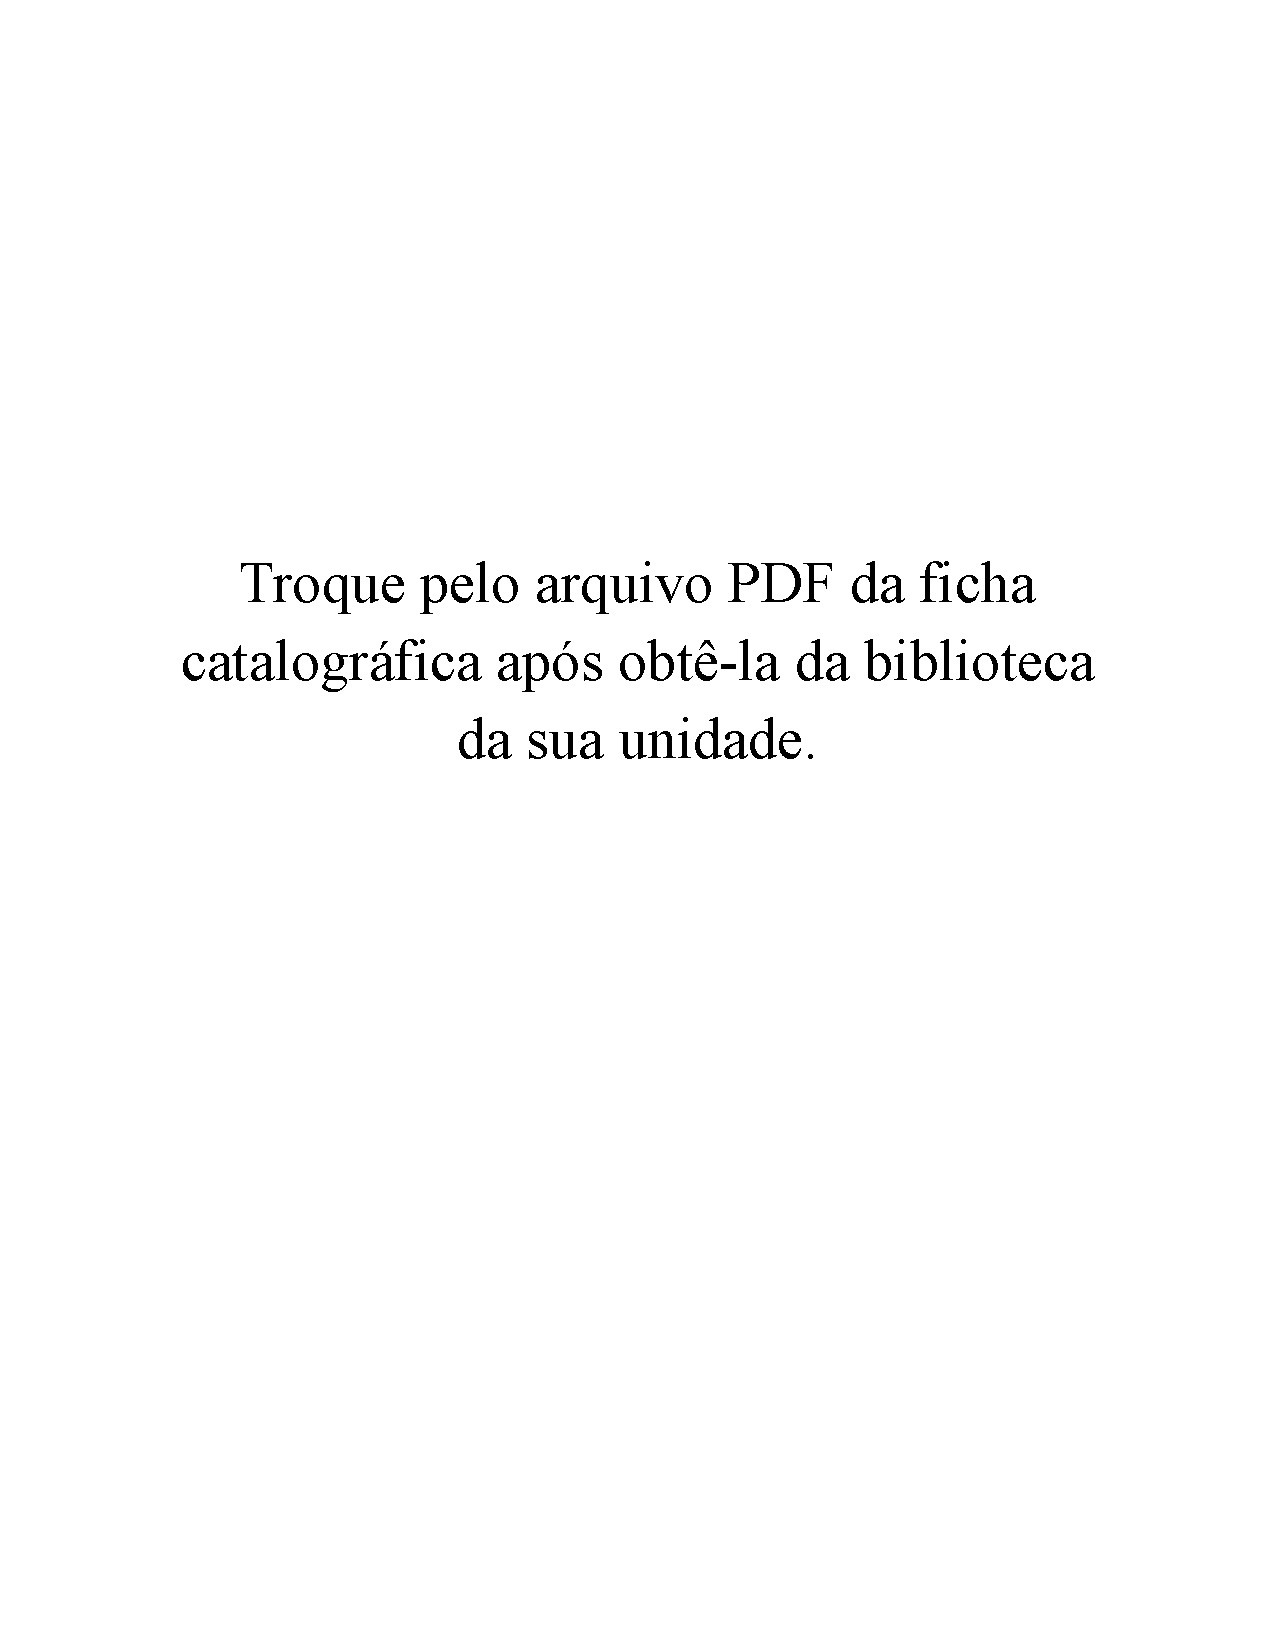
\includepdf{./pretextuais/fichacatalografica}

    % Folha de Aprovação/Ata de defesa: só para trabalhos de mestrado e 
    % doutorado. Caso a ata tenha 2 páginas, você alterar o parâmetro pages={1}
    % para pages={1-2}.	
    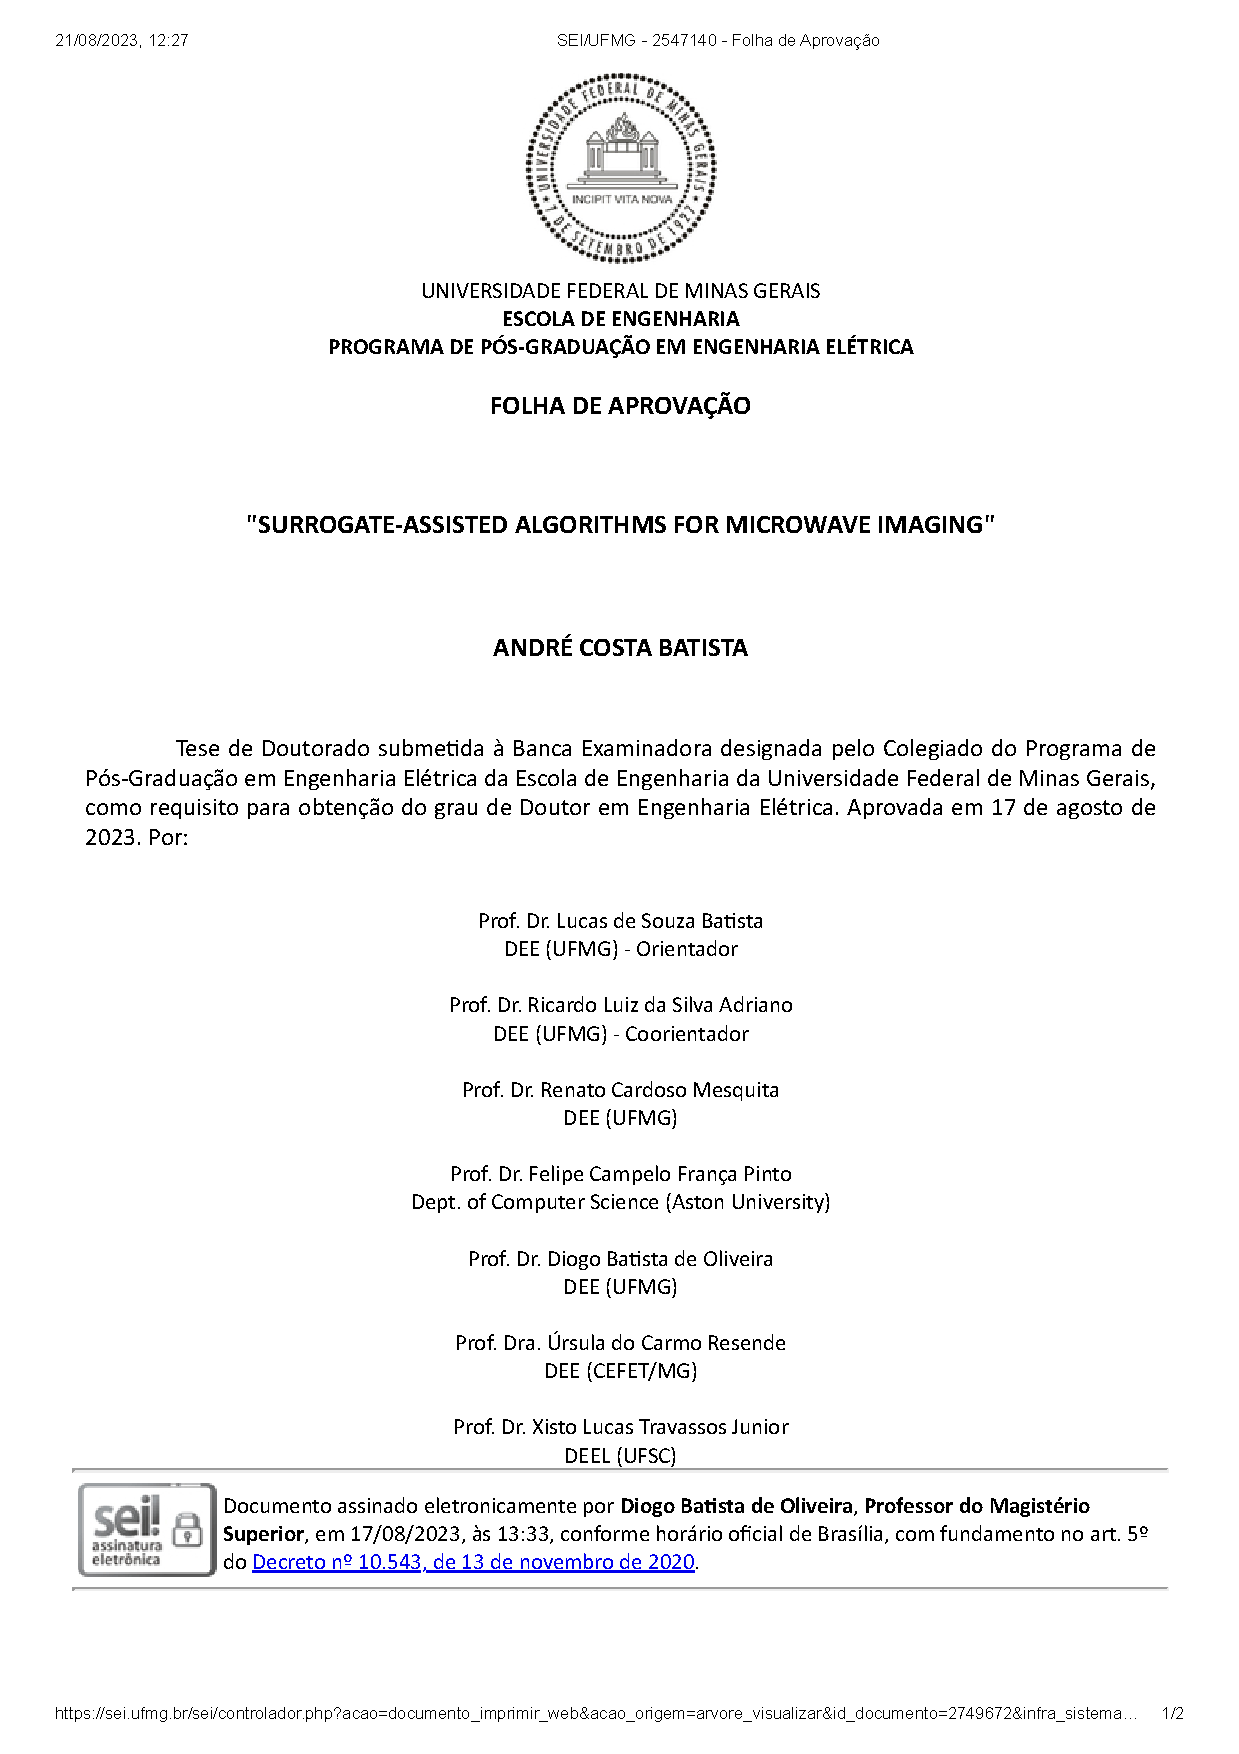
\includepdf[pages={1}]{./pretextuais/folhaaprovacao}

    % Dedicatória
    % A dedicatória, elemento opcional, é utilizada pelo autor para homenagear
% pessoa(s) a quem se dedica o trabalho. O texto é breve, apresentado ao final 
% da página com recuo de 8 cm à esquerda e a página não apresenta título.

\newpage
\thispagestyle{empty}
\vspace*{\fill}
\begin{flushright}
	\hspace{8cm}\textit{Esse trabalho é dedicado à aquela pessoa.}
\end{flushright}

    % Agradecimentos
	% s agradecimentos são destinados à menção de pessoas e instituições que 
% tenham contribuído para o desenvolvimento do trabalho.

\newpage

\chapter*{Agradecimentos} % Inglês: Acknowledgements

	Você pode escrever aqui os agradecimentos a pessoas que contribuíram para a realização do trabalho.
	
	\thispagestyle{empty}

    % Epígrafe
    % As epígrafes são empregadas quando o autor deseja apresentar uma citação 
% direta que estabelece relação com o trabalho apresentado. A página em que 
% consta, não apresenta título “Epígrafe”. Este recurso pode ser utilizado, 
% também, na abertura de cada uma das seções primárias do texto. 

\newpage
\thispagestyle{empty}
\vspace*{\fill}
\begin{flushright}
	``Aqui vai uma bela e inspiradora frase.''
\end{flushright}

    % Resumo e Abstract
	\chapter*{Resumo}

	\noindent O Imageamento em Microondas é uma importante técnica de teste e avaliação não-destrutiva e não-invasiva com muitas aplicações em diversas áreas, como em exames médicos, triagem de segurança, sensoriamento remoto, entre outras. A técnica é baseada em um Problema Inverso de Espalhamento Eletromagnético onde as propriedades elétricas de um meio são recuperadas através de medições de campo espalhado. Além de ser um problema mal-posto, também é não-linear e multimodal. Existem vários métodos numéricos para resolver o problema e eles podem ser classificados em qualitativos ou quantitativos. Estes últimos também são classificados em métodos determinísticos ou estocásticos. Esta tese apresenta uma nova abordagem quantitativa determinística para imageamento em microondas usando algoritmos assistidos por modelos substitutos. O objetivo é abordar os desafios do problema inverso considerando a imagem qualitativa recuperada pelo Método de Amostragem de Ortogonalidade e transformando a imagem em um problema de otimização bidimensional. O método proposto se concentra em otimizar a estimativa de contraste e a operação de limiarização para minimizar o erro da equação de dados. A tese apresenta três formulações baseadas em Algoritmos Evolutivos e duas baseadas em Métodos de Direções de Busca, fornecendo um leque de opções para a resolução do problema de otimização. Além disso, uma nova estrutura é proposta para o desenvolvimento e teste de algoritmos para o problema. A estrutura inclui um pacote abrangente chamado \textit{eispy2d}, que oferece funcionalidades como geração de conjuntos de teste com controle de parâmetros, uma coleção de indicadores de desempenho (incluindo dois novos indicadores) e suporte para comparação estatística de diferentes algoritmos. Os resultados dos experimentos demonstram a eficácia dos métodos propostos. Em cenários com espalhadores fracos, os métodos propostos foram capazes de reconstruir imagens comparáveis àquelas obtidas por métodos tradicionais, enquanto alcançavam tempos de execução próximos. Além disso, em cenários mais desafiadores onde os métodos tradicionais falharam, os algoritmos propostos mostraram resultados consistentes em termos de recuperação de imagens.

	\vspace{5mm}
	
	\noindent\textbf{Palavras-chaves}: imageamento em microondas; problemas inversos; algoritmos assistidos por modelos substitutos; algoritmos evolutivos; métodos de direção de busca; biblioteca de código aberto.
	
	\thispagestyle{empty}
    \chapter*{Abstract}

	\noindent Microwave Imaging is an important nondestructive and noninvasive testing and evaluating technique with many applications in diverse areas, such as medical imaging, security screening, remote sensing, among others. The technique is based on an Electromagnetic Inverse Scattering Problem where the electric properties of a medium are recovered through scattered field measurements. Besides being an ill-posed problem, it is also nonlinear and multimodal. There are several numerical methods for solving the problem and they can be classified into qualitative and quantitative ones. The latter is also classified into deterministic and stochastic methods. This thesis presents a novel quantitative deterministic approach for microwave imaging using surrogate model-assisted algorithms. The objective is to address the challenges of the inverse problem by considering the qualitative image recovered by the Orthogonality Sampling Method and transforming it into a two-dimensional optimization problem. The proposed method focuses on optimizing the contrast estimation and the threshold operation to minimize the data equation error. The thesis introduces three formulations based on Evolutionary Algorithms and two ones based on Descent Methods, providing a range of options for solving the optimization problem. In addition, a new framework is proposed for the development and testing of algorithms in microwave imaging. The framework includes a comprehensive package called \textit{eispy2d}, which offers functionalities such as test set generation with parameter control, a collection of performance indicators (including two novel indicators), and support for statistical comparison of different algorithms. The results of the experiments demonstrate the effectiveness of the proposed methods. In weak scatterer scenarios, the surrogate model-assisted algorithms were able to recover images that were comparable to those obtained by traditional methods, while achieving similar runtimes. Moreover, in more challenging scenarios where traditional methods failed, the proposed algorithms showed consistent results in terms of image recovery.
	
	\vspace{5mm}
	
	\noindent\textbf{Keywords}: microwave imaging; inverse problems; surrogate model-assisted algorithms; evolutionary algorithm; descent methods; open-source package.
	
	\thispagestyle{empty}
	

	% Listas
    \begingroup
    \pagestyle{empty}
    \listoffigures
    \pagestyle{empty}
    \listoftables
    \pagestyle{empty}
    \listofalgorithms
\endgroup
	
    % Abreviações e símbolos
	% Siglas e abreviaturas utilizadas no texto devem ser apresentadas em uma lista 
% alfabética seguida de sua grafia por extenso. A primeira vez que a sigla 
% aparece no texto deve-se pontuar a expressão por extenso, seguida da sigla 
% entre parênteses; nas demais vezes, utiliza-se somente a sigla, inserida
% diretamente no texto.

\newpage
\chapter*{Lista de Siglas e Símbolos} % Inglês: List of Abbreviations and Symbols

	\section*{Siglas}
	
		\begin{itemize}[labelwidth=5em,leftmargin=\dimexpr\labelwidth+\labelsep\relax,align=left]
			\item[ACO] Ant Colony Optimization
			\item[BIM] Born Iterative Method
			\item[CNN] Convolutional Neural Networks
			\item[DE] Differential Evolution
			\item[EA] Evolutionary Algorithm
			\item[GA] Genetic Algorithm
			\item[GAN] Generative Adversarial Network
			\item[PSO] Particle Swarm Optimization
			\item[TMz] Modo Magnético Transversal em $z$
		\end{itemize}
	
		\thispagestyle{empty}

	\section*{Símbolos}
	
		\thispagestyle{empty}
	
		\begin{itemize}[labelwidth=4em,leftmargin=\dimexpr\labelwidth+\labelsep\relax,align=left]
			\item[$\epsilon$] Permissividade complexa [F/m + $j\Omega$/m]
			\item[$\epsilon_r$] Permissividade relativa
			\item[$\theta$] Ângulo da coordenada polar [rad]
			\item[$\lambda_b $] Comprimento de onda de fundo [m]
			\item[$\sigma$] Condutividade [$\Omega$/m]
			\item[$\phi$] Ângulo de incidência [rad]
			\item[$\mathbf{E}$] Vetor de intensidade elétrica [V/m]
			\item[$E_z$] Componente $z$ do vetor de intensidade elétrica [V/m]
			\item[$k$] Número de onda [1/m]
			\item[$\mathbb{R}$] Conjunto dos números reais
			\item[$\mathbf{r}$] Vetor posição no espaço 3D [m]
			\item[$x, y, z$] Coordenadas cartesianas [m]
			\item[$V$] Espaço tridimensional
		\end{itemize}
	
		\thispagestyle{empty}
	
	
    
    % Sumário
    \thispagestyle{empty}
    \tableofcontents

    % Ativa numeração de páginas
    % ATENÇÃO: depois que você terminar de escrever o trabalho, você DEVE
    % voltar aqui acertar o número
    \pagenumbering{arabic}
    \setcounter{page}{12}

    % Introdução
    % ------------------------------------------------------------------------------
% Introdução
% ------------------------------------------------------------------------------

\chapter{Introdução}\label{chap:introducao} % Inglês: Introduction

	Parte inicial do texto na qual se apresenta a delimitação do assunto tratado, os 
	objetivos da pesquisa e outros elementos necessários para apresentar o tema 
	do trabalho. O texto tem o objetivo de introduzir o leitor ao trabalho e 
	apresentar as informações para uma compreensão geral da proposta
	desenvolvida.

	\section{Objetivos Geral e Específicos}\label{sec:introducao:objetivos}

		Descrever os objetivos geral e específicos do trabalho. O objetivo
		geral devem ser claro e conciso, indicando o propósito do trabalho.
		Os objetivos específicos devem ser apresentados de forma a indicar
		os passos necessários para atingir o objetivo geral. Geralmente, em formato de tópicos.

	\section{Contribuições e Originalidade}\label{sec:introducao:contribuicoes}

		Descrever as contribuições do trabalho, indicando o que o trabalho
		propõe de novo ou diferente em relação ao estado da arte. As contribuições
		devem ser claras e objetivas, indicando o que o trabalho agrega ao conhecimento
		existente.
	
	\section{Organização do Trabalho}\label{sec:introducao:organizacao}

		Descrever a organização do trabalho, indicando o conteúdo de cada capítulo
		e a relação entre eles. A organização do trabalho deve ser clara e
		coerente, de forma a facilitar a compreensão do leitor.



    % ------------------------------------------------------------------------------
% Problem Statement
% ------------------------------------------------------------------------------

\chapter{Problem Statement}\label{chap:problemstatement}

	%O Imageamento em Microondas é um problema inverso de espalhamento eletromagnético. Por ter essa natureza, sua grandezas são definidas em termos das equações de Maxwell as quais descrevem o fenômeno eletromagnético. Particularmente, o problema pode ser escrito em forma de uma equação integral, o que é muito comum para problemas que envolve radiação de uma corrente, seja ela impressa ou induzida. Ao invés de se determinar o efeito a partir de uma causa, o problema é definido de maneira inversa. Por causa disso, existem várias características peculiares para esse tipo problema que é considerado mal-posto na literatura.
	Microwave Imaging is an Electromagnetic Inverse Scattering Problem (EISP). Because of its nature, its magnitudes are defined in terms of Maxwell's equations which describe the electromagnetic phenomenon. In particular, the problem can be written in the form of an integral equation, which is very common for problems involving radiation from a current, whether impressed or induced. Rather than determining the effect from a cause, the problem is defined inversely. Thus, there are several characteristics peculiar to this kind of problem which is considered an ill-posed one in the literature.
	
	%Este capítulo tem por objetivo descrever de uma maneira geral o modelo matemático que representa o problema e discutir importantes aspectos associados. Primeiro, será apresentado a modelagem eletromagnética do problema para que, em seguida, seja desenvolvida a equação que relaciona todas as grandezas importantes para o problema. Posteriormente, alguns fundamentos sobre problemas inversos são apresentados. Logo após, vários aspectos importantes do problema são discutidos. Por fim, é apresentada uma conclusão destacando os principais pontos do capítulos. Também foram escritos os apêndices A, B e C como material de suporte para vários conceitos e deduções que serão utilizados nesse capítulo.
	This chapter aims to describe in a general way the mathematical model which represents the problem and to discuss its most important aspects. In Section \ref{chap:problemstatement:eletromagnetic}, the electromagnetic model will be presented. Then, in Section \ref{chap:problemstatement:integral}, the equation which relates all the required quantities will be developed. Subsequently, some fundamentals about inverse problems are presented in Section \ref{chap:problemstatement:inverse}. Afterward, several important aspects of the problem are discussed in Section \ref{chap:problemstatement:eisp}. Finally, a conclusion is presented highlighting the main topics of the chapter. Appendices \ref{app:green}, \ref{app:integral} and \ref{app:functional} were also written as supporting material for several concepts and deductions that will be used in this chapter.

	\section{Electromagnetic Theory}\label{chap:problemstatement:eletromagnetic}
	
		Maxwell's equations mathematically describe the electromagnetic phenomena. The four equations relate fields and sources in space and time. They are expressed as follows \citep{harrington2001}:
		\begin{eqnarray}
			\nabla\times\boldsymbol{\mathcal{E}}(\mathbf{r}, t) &=& - \frac{\partial\boldsymbol{ \mathcal{B}}}{\partial t}(\mathbf{r}, t) \label{eq:2:maxwell:time:1} \\
			\nabla\times\boldsymbol{\mathcal{H}}(\mathbf{r}, t) &=& \frac{\partial\boldsymbol{ \mathcal{D}}}{\partial t}(\mathbf{r}, t) + \boldsymbol{\mathcal{J}}(\mathbf{r}, t) \label{eq:2:maxwell:time:2} \\
			\nabla\cdot\boldsymbol{\mathcal{D}}(\mathbf{r}, t) &=& \rho(\mathbf{r}, t) \label{eq:2:maxwell:time:3} \\
			\nabla\cdot\boldsymbol{\mathcal{B}}(\mathbf{r}, t) &=& 0 \label{eq:2:maxwell:time:4}
		\end{eqnarray}
	
		The vector $\mathbf{r} = x\mathbf{x} + y\mathbf{y} + z\mathbf{z} = \langle x, y, z \rangle$ denotes the space coordinates (in meters [m])  and $t$ is the time (in seconds [s]). The vectors $\boldsymbol{\mathcal{E}}$, $\boldsymbol{\mathcal{H}}$, $\boldsymbol{\mathcal{D}}$, and $\boldsymbol{\mathcal{B}}$ represent electric field intensity (in volts per meter [V/m]), magnetic field intensity (in amperes per meter [A/m]), electric flux density (in coulombs per square meter [C/m$^2$]), and magnetic flux density (in tesla [T]). The sources are the electric current density $\boldsymbol{\mathcal{J}}$ (in amperes per square meter [A/m$^2$]) and the volume electric charge density $\rho$ (in coulombs per cubic meter [C/m$^3$]).
	
		Maxwell's equations can also be written in harmonic form, i.e., when time dependence is expressed in cosinusoidal form. In this case, the fields and sources can be written as quantities of a complex nature based on the following relationship:
		\begin{equation}
			\boldsymbol{\mathcal{F}}(\mathbf{r}, t) = \mathfrak{Re}\{\mathbf{F}(\mathbf{r})e^{j\omega t}\} \label{eq:2:fourier}
		\end{equation}
	
		In this way, the real vector field $\boldsymbol{\mathcal {F}}$ is completely described by the complex field $\mathbf{F}$ and the known angular frequency $\omega = 2\pi f$ (in radians per second [rad/s]). In \eqref{eq:2:fourier}, $j=\sqrt{-1}$ is the imaginary unit. Thus, Maxwell's equations in harmonic regime are defined as:
		\begin{eqnarray}
			\nabla\times\mathbf{E}(\mathbf{r}) &=& - j\omega\mathbf{B}(\mathbf{r}) \label{eq:2:maxwell:har:1} \\
			\nabla\times\mathbf{H}(\mathbf{r}) &=&  j\omega\mathbf{D}(\mathbf{r}) + \mathbf{J}(\mathbf{r}) \label{eq:2:maxwell:har:2} \\
			\nabla\cdot\mathbf{D}(\mathbf{r}) &=& \rho(\mathbf{r}) \label{eq:2:maxwell:har:3} \\
			\nabla\cdot\mathbf{B}(\mathbf{r}) &=& 0 \label{eq:2:maxwell:har:4}
		\end{eqnarray}
	
		In addition to Maxwell's equations, constitutive relationships are important for describing the relationship between fields and the environments in which they exist. In general, the relationships between field intensity and flux density vectors are expressed as:
		\begin{eqnarray}
			\mathbf{D}(\mathbf{r}) &=& F_1(\mathbf{E}, \mathbf{H})(\mathbf{r}) \label{eq:2:constitutive:general:1} \\
			\mathbf{B}(\mathbf{r}) &=& F_2(\mathbf{E}, \mathbf{H})(\mathbf{r}) \label{eq:2:constitutive:general:2}
		\end{eqnarray}
	
		The operators $F_1$ and $F_2$ represent the relationships between these two types of vector quantities. They are defined according to the medium in which these fields are present. Depending on the properties of each medium, these operators can be: linear or nonlinear; dependent on $\mathbf{E}$ and $\mathbf{H}$ or just one of these two vectors; defined as tensors or even scalars. Considering only linear, isotropic, and non-dispersive media, the constitutive relationships can be simplified to:
		\begin{eqnarray}
			\mathbf{D}(\mathbf{r}) &=& \epsilon_0\epsilon_r(\mathbf{r})\mathbf{E}(\mathbf{r}) \label{eq:2:constitutive:liniso:1} \\
			\mathbf{B}(\mathbf{r}) &=& \mu_0\mu_r(\mathbf{r})\mathbf{H}(\mathbf{r}) \label{eq:2:constitutive:liniso:2}
		\end{eqnarray}
	
		The constants $\epsilon_0$ and $\mu_0$ represent vacuum dielectric permittivity (in farads per meter [F/m]) and vacuum magnetic permeability (in henries per meter [H/m]), respectively. These constants are already known and are equivalent to $\epsilon_0\approx 8.854\times10^{-12}$ [F/m] and $\mu_0 = 4\pi\times10^{-7}$ [H/m]. The dimensionless quantities $\epsilon_r$ and $\mu_r$ represent the relative dielectric permittivity and magnetic permeability, i.e., they define the electromagnetic properties of a medium in proportion to the vacuum ones. They can be defined as functions which map their scalar value in space, either to delimit objects or to represent heterogeneities. In addition to these properties, if conductive objects are considered, the source $\mathbf{J}$ in \eqref{eq:2:maxwell:har:2} must be rewritten as the sum of an impressed current $\mathbf{J}_i $ and an induced one $\sigma\mathbf{E}$ defined by Ohm's law, i.e., $\mathbf{J}(\mathbf {r}) = \mathbf{J}_i (\mathbf{r}) + \sigma(\mathbf{r})\mathbf{E}(\mathbf{r})$. The electrical conductivity $\sigma$ (in siemens per meter [S/m]) is the property that describes the ability of the medium to induce current in the presence of an electric field. From this definition, \eqref{eq:2:maxwell:har:2} can be rewritten as:
		\begin{eqnarray}
			\nabla\times\mathbf{H}(\mathbf{r}) &=&  j\omega\epsilon_0\epsilon_r\mathbf{E}(\mathbf{r}) + \sigma(\mathbf{r})\mathbf{E}(\mathbf{r})+ \mathbf{J}_i(\mathbf{r}) \label{eq:2:complexmedia:1} \\
			 &=&  j\omega\epsilon_0\left(\epsilon_r(\mathbf{r}) -j\frac{\sigma(\mathbf{r})}{\omega\epsilon_0}\right)\mathbf{E}(\mathbf{r}) +  \mathbf{J}_i(\mathbf{r}) \label{eq:2:complexmedia:2} \\
			&=&  j\omega\epsilon(\mathbf{r})\mathbf{E}(\mathbf{r}) +  \mathbf{J}_i(\mathbf{r}) \label{eq:2:complexmedia:3}
		\end{eqnarray}
	
		The quantity $\epsilon = \epsilon_0\epsilon_r - j\sigma/\omega$ is called effective dielectric permittivity and is a complex scalar.
	
	\section{Integral Equations}\label{chap:problemstatement:integral}
	
		The scattering problem consists of a source $\mathbf{J}_i(\mathbf{r})$ which propagates a wave through a medium with electromagnetic properties $\epsilon_b$ and $\mu_b$ and in the presence of a non-homogeneous scatter with properties $\epsilon(\mathbf{r})$ and $\mu(\mathbf{r})$ (Figure \ref{fig:2:scattering}) \citep{chew1995}. In this scenario, the equations \eqref{eq:2:maxwell:har:1}-\eqref{eq:2:maxwell:har:4} are valid for any point $\mathbf{r}$ of space. With the aid of \eqref{eq:2:constitutive:liniso:2}, the equation \eqref{eq:2:maxwell:har:1} can be rewritten as:
		\begin{eqnarray}
				\nabla\times\mathbf{E}(\mathbf{r}) &=& - j\omega\mu(\mathbf{r})\mathbf{H}(\mathbf{r}) \label{eq:2:waveequations:1} \\
				\mu^{-1}(\mathbf{r})\nabla\times\mathbf{E}(\mathbf{r}) &=& - j\omega\mathbf{H}(\mathbf{r}) \label{eq:2:waveequations:2} 
		\end{eqnarray}
	
	    \begin{figure}[!tb]
			\centering
			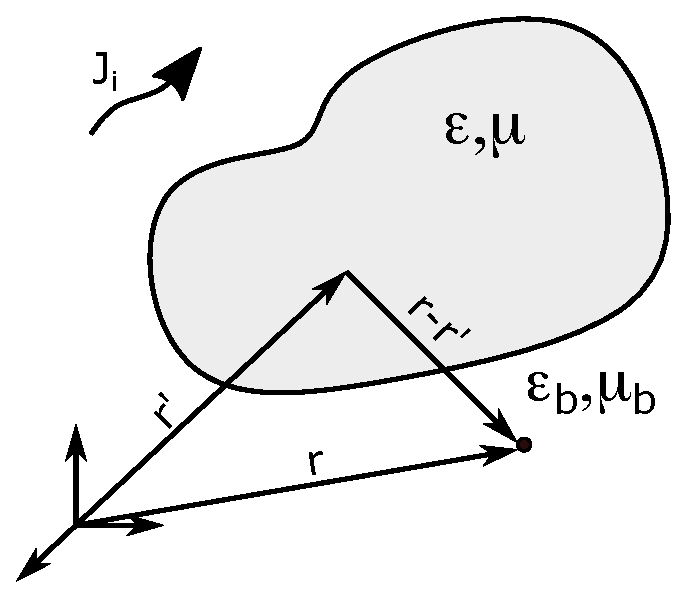
\includegraphics[width=0.5\textwidth]{./figuras/scattering}
			\caption{General scattering problem.}
			\label{fig:2:scattering}
		\end{figure}
	
		If we take the curl of \eqref{eq:2:waveequations:2}, we can use \eqref{eq:2:complexmedia:3} to obtain an equation with only the electric field:
		\begin{eqnarray}
			\nabla\times\mu^{-1}(\mathbf{r})\nabla\times\mathbf{E}(\mathbf{r}) &=& - j\omega\nabla\times\mathbf{H}(\mathbf{r}) \label{eq:2:waveequations:3} \\ \nabla\times\mu^{-1}(\mathbf{r})\nabla\times\mathbf{E}(\mathbf{r}) &=& - j\omega\left(j\omega\epsilon(\mathbf{r})\mathbf{E}(\mathbf{r}) +  \mathbf{J}_i(\mathbf{r})\right) \label{eq:2:waveequations:4}
		\end{eqnarray}
	
		Through this, we obtain the vector wave equation:
		\begin{equation}
					\nabla\times\mu^{-1}(\mathbf{r})\nabla\times\mathbf{E}(\mathbf{r}) - \omega^2\epsilon(\mathbf{r})\mathbf{E}(\mathbf{r})  = - j\omega\mathbf{J}_i(\mathbf{r}) \label{eq:2:waveequations:5} 
		\end{equation}
	
		Subtracting both sides of \eqref{eq:2:waveequations:5} by $\nabla\times\mu_b^{-1}\nabla\times\mathbf{E}(\mathbf{r})-\omega^2\epsilon_b\mathbf{E}(\mathbf{r})$, one can obtain:
		\begin{multline}
			\nabla\times\left(\mu^{-1}(\mathbf{r})-\mu_b^{-1}\right)\nabla\times\mathbf{E}(\mathbf{r}) - \omega^2\left(\epsilon(\mathbf{r})-\epsilon_b\right)\mathbf{E}(\mathbf{r}) \\ =  -  j\omega\mathbf{J}_i(\mathbf{r}) -\nabla\times\mu_b^{-1}\nabla\times\mathbf{E}(\mathbf{r}) + \omega^2\epsilon_b\mathbf{E}(\mathbf{r}) \label{eq:2:waveequations:6}
		\end{multline}
		\begin{multline}
			\nabla\times\mu_b^{-1}\nabla\times\mathbf{E}(\mathbf{r}) - \omega^2\epsilon_b\mathbf{E}(\mathbf{r}) \\ = -j\omega\mathbf{J}_i(\mathbf{r}) + \omega^2\left(\epsilon(\mathbf{r})-\epsilon_b\right)\mathbf{E}(\mathbf{r}) -	\nabla\times\left(\mu^{-1}(\mathbf{r})-\mu_b^{-1}\right)\nabla\times\mathbf{E}(\mathbf{r}) \label{eq:2:waveequations:7} 
		\end{multline}
	
		The right side of \eqref{eq:2:waveequations:7} represents the effective current source $\mathbf{J}$. This equation is analogous to the problem described in \autoref{app:integral}. Therefore, similarly to \eqref{eq:app:integral:final}, the solution of \eqref{eq:2:waveequations:7} is:
		\begin{multline}
			\mathbf{E}(\mathbf{r}) =  j\omega \int_V d\mathbf{r^\prime}~ \mathbf{\bar{G}}(\mathbf{r},\mathbf{r^\prime})\cdot\mu_b\mathbf{J}(\mathbf{r}) + \omega^2\int_V d\mathbf{r^\prime}~\mathbf{\bar{G}}(\mathbf{r},\mathbf{r^\prime})\cdot\mu_b\left(\epsilon(\mathbf{r^\prime})-\epsilon_b\right)\mathbf{E}(\mathbf{r^\prime}) \\ - \int_V d\mathbf{r^\prime}~\mathbf{\bar{G}}(\mathbf{r},\mathbf{r^\prime})\cdot\mu_b\nabla^\prime\times\left(\mu^{-1}(\mathbf{r^\prime})-\mu_b^{-1}\right)\nabla^\prime\times\mathbf{E}(\mathbf{r^\prime}) \label{eq:2:waveequations:8}
		\end{multline}
	
		The first term on the right side of \eqref{eq:2:waveequations:8} is the field produced by the impressed source of the problem, which is also called the incident field $\mathbf{E}_i(\mathbf{r})$. The function $\mathbf{\bar{G}}(\mathbf{r},\mathbf{r^\prime})$ is the Dyadic Green's Function for homogeneous medium \eqref{eq:app:green:17} and it is the impulse response, i.e., the solution of the equations for a point source (see Appendix \ref{app:green} for further information). The second term represents the field due to the displacement or conduction electric currents, while the third term represents the field due to the magnetic polarization charges. If we suppose that there are only non-magnetic materials, i.e., $\mu = \mu_b = \mu_0$, then we can rewrite \eqref{eq:2:waveequations:8} as:
		\begin{equation}
			\mathbf{E}(\mathbf{r}) = \mathbf{E}_i(\mathbf{r}) + k_b^2\int_V d\mathbf{r^\prime}~\mathbf{\bar{G}}(\mathbf{r},\mathbf{r^\prime})\cdot\chi(\mathbf{r^\prime})\mathbf{E}(\mathbf{r^\prime}) \label{eq:2:waveequations:final}
		\end{equation}
	
		\noindent in which:
		\begin{equation}
			\chi(\mathbf{r}) = \frac{\epsilon_r(\mathbf{r})}{\epsilon_{rb}}-1-j\frac{\sigma(\mathbf{r})-\sigma_b}{\omega\epsilon_b} \label{eq:2:contrast}
		\end{equation}
	
		\noindent is called the contrast function and $k_b = \omega\sqrt{\mu_0\epsilon_b}$ is the background wavenumber (in meters [m]).
	
	\section{Basic Theory of Inverse Ill-Posed Problems}\label{chap:problemstatement:inverse}
	
		%Para um dado fenômeno nós conhecemos a causa e procuramos conhecer o efeito, estamos lidando com um problema direto. Por um outro lado, se conhecemos o efeito e procuramos a causa, estamos lidando com um problema inverso. Alternativamente, existem outras maneiras de se definir um problema inverso. Conforme definiu \cite{keller1976inverse}, dois problemas são inversos entre si se a formulação de cada uma envolve a solução completa da outra. Além disso, conforme afirmado também por \cite{bertero2020introduction}, no passado, os problemas diretos foram amplamente estudados enquanto os inversos não eram e eram pouco entendidos. Com frequência, os problemas inversos eram também mal-postos.
		There is no rigorous mathematical definition of inverse problems. In fact, when someone defines a problem as the inverse counterpart of some other, this is usually arbitrary. A very known definition was written by \cite{keller1976inverse} in which two problems are inverse to each other if the formulation of each involves the complete solution of the other. Also, as stated by \cite{bertero2020introduction}, the direct problem used to be the one that had been extensively studied while the inverse counterpart used to be one that was still poorly understood. From a physical perspective, for a given phenomenon, if the cause is known and we attempt to know the effect, then we are dealing with a direct or forward problem. On the other hand, if the effect is known and the cause is sought, then we are dealing with an inverse problem.
	
		%\cite{hadamard1923lectures} definiu que um modelo matemático para um problema físico seria bem-posto ou propriamente posto se três condições fossem garantidas. De uma forma matemática, sendo $X$ e $Y$ espaços normais e $\mathcal{K}$ um operador linear ou não no qual $\mathcal{K} : X \rightarrow Y$, a equação $\mathcal{K}\{x\}=y$ é bem-posta se \citep{kirsch2011introduction}:
		One of the reasons for inverse problems being the least attractive one is that they are often ill-posed. \cite{hadamard1923lectures} defined that a mathematical model for a physical problem would be well-posed or properly posed if three conditions were guaranteed. Mathematically, let $X$ and $Y$ be normed spaces and $\mathcal{K}$ a linear or nonlinear operator in which $\mathcal{K} : X \rightarrow Y$, the equation $\mathcal{K}\{x\}=y$ is well-posed if \citep{kirsch2011introduction}:
		\begin{enumerate}
			%\item \textbf{Existência}: para cada $y\in Y$ existe pelo menos um $x\in X$ no qual $\mathcal{K}\{x\}=y$;
			\item \textbf{Existence}: for each $y\in Y$ there is at least one $x\in X$ in which $\mathcal{K}\{x\}=y$;
			%\item \textbf{Unicidade}: para cada $y\in Y$ existe no máximo um $x\in X$ no qual $\mathcal{K}\{x\}=y$;
			\item \textbf{Uniqueness}: for each $y\in Y$ there is at most one $x\in X$ in which $\mathcal{K}\{x\}=y$;
			%\item \textbf{Estabilidade}: a solução $x$ tem dependência contínua em relação a $y$, i.e., para cada sequência $(x_n)\subset X$ no qual $\mathcal{K}\{x_n\}\rightarrow \mathcal{K}\{x\}$ quando $n\rightarrow\infty$, segue-se $x_n\rightarrow x$ quando $n\rightarrow\infty$.
			\item \textbf{Stability}: solution $x$ has continuous dependence on $y$, i.e., for each sequence $(x_n)\subset X$ in which $\mathcal{K}\{x_n\}\rightarrow \mathcal{K}\{x\}$ when  $n\rightarrow\infty$, follows $x_n\rightarrow x$ when $n\rightarrow\infty$ .
		\end{enumerate}
	
		%Quando um problema não atende pelo menos uma dessas condições, então ele é chamado de mal-posto ou impropriamente posto. Entretanto, quando alguma delas é violada, é possível adotar algumas estratégias para que a posição do problema seja corrigida. Por exemplo, quando não existe solução, o espaço de soluções pode ser alargado para que o respectivo critério seja atendido. Quando há muitas soluções, então pode estar faltando alguma informação que restrinja o espaço e garanta a unicidade de solução. No entanto, quando o problema não é estável, então é praticamente impossível encontrar a solução a menos que novas informações sobre ela sejam adicionadas. Conforme afirmado por \cite{lanczos1961linear}, quando se falta informação, não existe artifiício matemático que possa consertar.
		When a problem does not satisfy at least one of these conditions, then it is called ill-posed or improperly posed. However, when any of them is violated, it is possible to adopt some strategies so that the posedness conditions are fulfilled. For example, when there is no solution, the space of solutions can be enlarged so that the respective criterion is satisfied. When there are many solutions, then there may be a lack of information which could reduce space and ensures uniqueness. However, when the problem is not stable, then it is practically impossible to find a solution unless a new information about its form is added. As stated by \cite{lanczos1961linear}, when information is lacking, there is no mathematical trickery that can fix it.
	
		%Além disso, as condições de existência e de unicidade dependem somente da natureza dos espaços e dos operadores. Já a condição de estabilidade depende também da topologia dos espaços, i.e., se o operador inverso $\mathcal{K}^{-1}:X\rightarrow Y$ é contínuo. Essas características estão relacionadas entre si, por exemplo, um operador inverso $\mathcal{K}^{-1}$ é automaticamente contínuo se $\mathcal{K}$ é linear e contínuo e $X$ e $Y$ são espaços de Banach\footnote{Um espaço normal $X$ sobre $\mathbb{R}$ ou $\mathbb{C}$ é chamado completo ou de Banach se toda sequência de Cauchy converge em $X$.}. Ademais, se $\mathcal{K}$ é um operador contínuo e compacto, o problema inverso é mal-posto a não ser que $X$ tenha dimensão finita \citep{colton2019inverse}.
		Besides, the conditions of existence and uniqueness depend only on the nature of the spaces and the operators. The stability condition also depends on whether the operator $\mathcal{K}:X\rightarrow Y$ is surjective. Continuity of the inverse operator $\mathcal{K}^{-1}:Y\rightarrow X$ is also relevant information. For example, an inverse operator $\mathcal{K}^{-1}$ is automatically continuous if $\mathcal{K}$ is linear and continuous and $X$ and $Y$ are Banach spaces (\autoref{def:app:functional:5}). Furthermore, if $\mathcal{K}$ is a continuous and compact operator, the inverse problem is ill-posed unless $X$ is of finite dimension \citep{colton2019inverse}.
		
		%A adição de informações para resolver problemas mal-postos pode ser alcançadas através de estratégias de regularização. Em problemas onde $X$ e $Y$ são espaços de Hilbert\footnote{Um espaço pré-Hilbert é um espaço com um produto interno definido. Um espaço de Hilbert é um espaço pré-Hilbert completo.}, $\mathcal{K}$ é um operador que é linear, compacto\footnote{Um conjunto relativamente compacto é aquele no qual cada sequência tem um ponto de acumulação. Um operador é denominado compacto se mapeia cada conjunto limitado em um conjunto relativamente compacto.} e um-pra-um\footnote{Um operador um-pra-um é aquele que injetivo e surjetivo, i.e., tem solução e única.}; e $y\in Y$ não é conhecido senão por um erro $\delta>0$ tal que:
		The addition of information to solve ill-posed problems can be achieved through regularization strategies. In problems where $X$ and $Y$ are Hilbert spaces, $\mathcal{K}$ is an operator that is linear, compact\footnote{In few words, the compactness of an operator means that its has infinitely small singular values accumulating at zero. A more precise definition is available at \autoref{def:app:functional:7}.}, and one-to-one; and $y\in Y$ is not known except for an error $\delta>0$ such that:
		\begin{equation}
			||y-y^\delta|| \le \delta \label{eq:2:inverse:1}
		\end{equation} 
	
		% \noindent no qual $y^\delta\in Y$. A equação $\mathcal{K}\{x^\delta\}=y^\delta$ geralmente não tem solução, uma vez que $y^\delta$ não está no intervalo $\mathcal{K}(X)$ de $X$. Então, o objetivo seria determinar uma solução $x^\delta\in X$ que se aproxima de $x\in X$. Além disso, é necessário que $x^\delta$ tenha dependência contínua em relação aos dados $y^\delta$. Portanto, o objetivo é contrauir um operador $\mathcal{R}_\alpha : Y \rightarrow X$ linear e limitado que seja uma aproximação de $\mathcal{K}^{-1}$, i.e.:
		\noindent where $y^\delta\in Y$.
		
		The equation $\mathcal{K}\{x^\delta\}=y^\delta$ usually has no solution since $y^\delta$ is not in the range $\mathcal{K}(X)$ of $X$. So, the goal would be to determine a solution  $x^\delta\in X$ that approximates $x\in X$. In addition, $x^\delta$ must depend continuously on the data $y^\delta$. Therefore, the objective is to construct a linear and bounded operator $\mathcal{R}_\alpha : Y \rightarrow X$ that is an approximation of $\mathcal{K}^{-1}$, i.e.:
		\begin{equation}
			\lim\limits_{\alpha\rightarrow0} \mathcal{R}_\alpha\{y\} = x,~\forall x \in X \label{eq:2:inverse:2}
		\end{equation}
	
		%Em outras palavras, o operador $\mathcal{R}_\alpha$ é tal que converge ponto-a-ponto para um operador identidade. Através dessa definição, $x^{\alpha, \delta} = \mathcal{R}_\alpha\{y^\delta\}$ é uma aproximação para a solução $x$ de $\mathcal{K}\{x\}=y$. Uma discussão mais profunda pode ser encontrados em livros sobre análise funcional e regularizadores \citep{kirsch2011introduction,lebedev1996functional}.
		In other words, the $\mathcal{R}_\alpha\{\mathcal{K}\{\cdot\}\}$ operation is such that it converges pointwise to an identity operator. Through this definition, $x^{\alpha, \delta} = \mathcal{R}_\alpha\{y^\delta\}$ is an approximation to the solution $x$ of $\mathcal{K}\{x\}=y$. A more in-depth discussion can be found in books on functional analysis and regularization strategies \citep{kirsch2011introduction,lebedev1996functional}.
	
	\section{The Eletromagnetic Inverse Scattering Problem}\label{chap:problemstatement:eisp}
	
		%Até aqui foram apresentadas os fundamentos para o problema inverso de espalhamento eletromagnético. Esta seção apresenta define o problema apresentando várias formulações possíveis, tanto na representação geral tridimensional quanto num caso particular bidimensional do modo tranversal magnético. Além disso, discussões sobre importantes aspectos do problema são elaboradas, tais como os espaços vetoriais das funções, unicidades, estabilidade, não-linearidade e graus de liberdade.
		So far, the fundamentals for EISP have been introduced. This section presents the problem by describing several possible formulations, both in the general three-dimensional representation and in a particular two-dimensional case (Transverse Magnetic mode). In addition, discussions about important aspects of the problem are elaborated, such as the vector spaces of functions, uniqueness, stability, non-linearity, and degrees of freedom.
	
		\subsection{Formulations}\label{chap:problemstatement:eisp:1}
			%A equação descreve o campo elétrico total observado em ponto através da soma de uma componente incidente e uma outra componente causada as correntes de indução. A esta última componente, denominamos de campo espalhado $\mathbf{E}_s$. Ou seja, a \eqref{eq:2:waveequations:final} pode ser reescrita como:
			The equation \eqref{eq:2:waveequations:final} describes the total electric field through the sum of an incident component and another one caused by induced currents. This latter component is called the scattered field $\mathbf{E}_s$. Particularly, \eqref{eq:2:waveequations:final} can be rewritten as:
			\begin{equation}
				\mathbf{E}(\mathbf{r}) = \mathbf{E}_i(\mathbf{r}) + \mathbf{E}_s(\mathbf{r}) \label{eq:2:eisp:1}
			\end{equation}
	
			\noindent where:
			\begin{equation}
				\mathbf{E}_s(\mathbf{r}) = k_b^2\int_V d\mathbf{r^\prime}~\mathbf{\bar{G}}(\mathbf{r},\mathbf{r^\prime})\cdot\chi(\mathbf{r^\prime})\mathbf{E}(\mathbf{r^\prime}) \label{eq:2:eisp:2}
			\end{equation}
		
			%Quando a função contraste $\chi$ e o campo incidente $\mathbf{E}_i$ são conhecidos dentro de uma região $V$,  o campo total $\mathbf{E}$ pode ser determinado através da equação \eqref{eq:2:waveequations:final}. Este problema é chamado de problema direto. Por um outro lado, se o campo espalhado $\mathbf{E}_s$ é conhecido em um ou um conjunto de pontos $\mathbf{r}$, geralmente fora de $V$, a equação \eqref{eq:2:eisp:2} pode ser utilizada para determinar-se $\chi$. A este problema denominamos de problema inverso de espalhamento (EISP). No entanto, é necessário observar que o campo total na região $V$ também é desconhecido e depende de $\chi$. Desta forma, EISP é um problema não-linear.
			When the contrast function $\chi$ and the incident field $\mathbf{E}_i$ are known within a region $V$, the total field $\mathbf{E}$ can be determined using equation \eqref{eq:2:waveequations:final}. This problem is called the forward or direct problem and the equation \eqref{eq:2:waveequations:final} is an example of a Fredholm Integral Equation of Second Kind \citep{polyanin2008handbook}. On the other hand, if the scattered field $\mathbf{E}_s$ is known at one or a set of points $\mathbf{r}$, usually outside $V$, equation \eqref{eq:2:eisp:2} can be used to determine $\chi$. We call this problem the Electromagnetic Inverse Scattering Problem (EISP). However, it is necessary to note that the total field in $V$ is also unknown and depends on $\chi$. Thus, EISP is a non-linear problem.
			
			%Em EISPs, a equação \eqref{eq:2:eisp:2} é chamada de equação de dados, uma vez que relaciona os dados do problema ($\mathbf{E}_s$) com as variáveis desconhecidas ($\chi$ e $\mathbf{E}$). Ela pode ser escrita na forma de um operador não-linear:
			In EISPs, equation \eqref{eq:2:eisp:2} is called data equation, since it relates the problem data ($\mathbf{E}_s$) with the unknown variables  ($\chi$ and $\mathbf{E}$). This equation belongs to a class called Lippman-Schwinger integral equations \citep{lippmann1950variational}. It can be written in the form of a non-linear operator:
			\begin{equation}
				\mathbf{E}_s(\mathbf{r}) = \mathcal{L}^D\left\{\chi(\mathbf{r^\prime}), \mathbf{E}(\mathbf{r^\prime})\right\},~\mathbf{r}\notin V,~ \mathbf{r^\prime}\in V \label{eq:2:eisp:3}
			\end{equation}
			
			%A equação \eqref{eq:2:waveequations:final} também é utilizada em EISPs e é conhecida como equação de estados. Ela é uma relação entre as variáveis desconhecidas ($\chi$ e $\mathbf{E}$) com uma conhecida a qual é uma entrada geral para o problema ($\mathbf{E}_i$). Também é possível escrever \eqref{eq:2:waveequations:final} em termos de um operador:
			The equation \eqref{eq:2:waveequations:final} is also used in EISPs and is known as the state equation. It is a relationship between unknown variables ($\chi$ and $\mathbf{E}$) with a known one which is a general entry for the problem ($\mathbf{E}_i$). It is also possible to write \eqref{eq:2:waveequations:final}  in terms of an operator:
			\begin{equation}
				\mathbf{E}_i(\mathbf{r}) = \mathbf{E}(\mathbf{r}) - \mathcal{L}^S\left\{\chi(\mathbf{r}), \mathbf{E}(\mathbf{r})\right\}, \mathbf{r}\in V \label{eq:2:eisp:4}
			\end{equation}
		
			%Assim como $\mathcal{L}^D$, $\mathcal{L}^S : U, W \rightarrow W$. Geralmente, esta equação é utilizada em situações onde $\mathbf{r}\in V$, i.e., o operador $\mathcal{L}^D$ pode envolver singularidades. No entanto, existem formas de abordar singularidades nessa equação (confira a seção \ref{app:green:2} do \autoref{app:green}).
			Frequently, this equation is used in situations where $\mathbf{r}\in V$, i.e., the $\mathcal{L}^S$ operator can involve singularities. However, there are approaches to address singularities in this equation (see \autoref{app:green} section \ref{app:green:2}).
			
			%Alternativamente, também é muito encontrado na literatura a formulação do EISP em termos da fonte de contraste $\mathbf{J}_{eq}(\mathbf{r}) = \chi(\mathbf{r})\mathbf{E}(\mathbf{r})$:
			Alternatively, the EISP formulation in terms of the contrast source $\mathbf{J}_{eq}(\mathbf{r}) = \chi(\mathbf{r})\mathbf{E}(\mathbf{r})$ is also widely found in the literature \cite{berg1997constrast}:
			\begin{eqnarray}
				\mathbf{E}_s(\mathbf{r}) &=& k_b^2\int_V d\mathbf{r^\prime}~\mathbf{\bar{G}}(\mathbf{r},\mathbf{r^\prime})\cdot\mathbf{J}_{eq}(\mathbf{r^\prime}) \label{eq:2:eisp:5} \\
				\chi(\mathbf{r})\mathbf{E}_i(\mathbf{r}) &=& \mathbf{J}_{eq}(\mathbf{r}) - k_b^2\chi(\mathbf{r})\int_V d\mathbf{r^\prime}~\mathbf{\bar{G}}(\mathbf{r},\mathbf{r^\prime})\cdot\mathbf{J}_{eq}(\mathbf{r^\prime}) \label{eq:2:eisp:6}
			\end{eqnarray}
		
			%A vantagem desse tipo de formulação é os operadores $\mathcal{L}^D$ e $\mathcal{L}^S$ são lineares. No entanto, ainda existem duas variáveis desconhecidas no problema ($\chi$ e $\mathbf{J}_{eq}$) as quais estão relacionadas de maneira não-linear na \eqref{eq:2:eisp:6}.
			The advantage of this type of formulation is that the $\mathcal{L}^D$ and $\mathcal{L}^S$ operators are linear. However, there are still two unknown variables in the problem ($\chi$ and $\mathbf{J}_{eq}$) that are related in a non-linear fashion in \eqref{eq:2:eisp:6}.
	
			%Também podemos destarcar formas alternativas de se escrever as integrais presentes em \eqref{eq:2:waveequations:final} e \eqref{eq:2:eisp:2} a partir de manipulações com os operadores presentes da função diádica de Green. Esses tipos de manipulações podem ser úteis para facilitar a implementação computacional das equações integrais. Uma manipulação muito comum é mover um dos operadores $\nabla$ dentro da função de Green para fora da integral. A vantagem desse tipo de técnica é reduzir o erro numérico de quadratura. Conforme mostrado na seção 4.4.1 de \citep{chew2009}, se considerarmos a equação \eqref{eq:app:green:12}, a qual representa as integrais em \eqref{eq:2:waveequations:final} e \eqref{eq:2:eisp:2}, a integral pode ser reescrita como:
			There are alternative forms of writing the integrals in \eqref{eq:2:waveequations:final} and \eqref{eq:2:eisp:2} through manipulating the derivative operators of dyadic Green's function. These kinds of manipulations can be convenient to facilitate the computational implementation of integral equations. A very common manipulator is to move one of the $\nabla$ operators within Green's function to the integral. The advantage of this technique is that it reduces the numerical quadrature error. As stated in section 4.4.1 of \cite{chew2009}, if we consider equation \eqref{eq:app:green:12}, which represents the integrals in \eqref{eq:2:waveequations:final} and \eqref{eq:2:eisp:2}, the integral can be rewritten as:
			\begin{eqnarray}
				\int_Vd\mathbf{r^\prime}g(\mathbf{r^\prime}-\mathbf{r})\left[\mathbf{\bar{I}}+\frac{\nabla^\prime\nabla^\prime}{k^2_b}\right]\cdot\chi(\mathbf{r^\prime})\mathbf{E}(\mathbf{r^\prime}) &=& \int_Vd\mathbf{r^\prime}g(\mathbf{r^\prime}-\mathbf{r})\chi(\mathbf{r^\prime})\mathbf{E}(\mathbf{r^\prime})\nonumber\\
				&+& \frac{\nabla}{k_b^2}\int_Vd\mathbf{r^\prime}g(\mathbf{r^\prime}-\mathbf{r})\nabla^\prime\cdot\chi(\mathbf{r^\prime})\mathbf{E}(\mathbf{r^\prime}) \label{eq:2:eisp:7}
			\end{eqnarray}
		
			%Alternativamente, ao invés da equação ser escrita em termos de um produto escalar do operador $\nabla$, ela também pode ser escrita em termos de um produto vetorial. Esta formulação pode ser interessante para determinadas formas de discretização do problema. Conforme descrito por \cite{chew2009}, a equação integral pode ser escrita como:
			Alternatively, instead of the equation being written in terms of a tensor product of the $\nabla$ operator, it can also be written in terms of a vector product. This formulation can be interesting for certain forms of discretization of the equation. As described by \cite{chew2009}, the integral equation can be written as:
			\begin{eqnarray}
				\epsilon(\mathbf{r})\mathbf{E}(\mathbf{r}) &=& \mathbf{E}_i(\mathbf{r}) - \nabla\times\int_Vd\mathbf{r^\prime}g(\mathbf{r^\prime}-\mathbf{r})\nabla^\prime\times\chi(\mathbf{r^\prime})\mathbf{E}(\mathbf{r^\prime}) \label{eq:2:eisp:8}
			\end{eqnarray}
		
			%Em todas essas formulações, as interações mútuas entre espalhadores são responsáveis pela natureza não-linear do problema.  Para mitigar os efeitos da não-linearidade, algumas reformulações já foram propostas na literatura \citep{bevacqua2021quantitative}. Uma delas é baseada na exploração do comportamento de pico da função de Green quando existem perdas no meio de fundo, i.e., seu objetivo é extrair parte da contribuição dominante da corrente. Através de algumas manipulações, a formulação chamada Contrast-Source Extended Born Model reescreve a equação de estados conforme se segue:
			%In all of these formulations, the mutual interactions between scatterers are responsible for the non-linear nature of the problem. However, some reformulations have already been proposed in the literature to mitigate the effects of nonlinearity \citep{bevacqua2021quantitative}. One of them is based on exploring the peak behavior of the Green's function when there are losses in the background medium, i.e., its objective is to extract part of the dominant current contribution. Through some manipulations, the formulation called Contrast-Source Extended Born Model rewrites the state equation as follows \citep{durso2010solution}:
			\begin{equation}
				\mathbf{J}_{eq}(\mathbf{r}) = p(\mathbf{r})\mathbf{E}_i(\mathbf{r}) + p(\mathbf{r})\left(  k_b^2\int_Vd\mathbf{r^\prime} \mathbf{\bar{G}}(\mathbf{r},\mathbf{r^\prime})\cdot\mathbf{J}_{eq}(\mathbf{r^\prime}) - \mathbf{f}_d(\mathbf{\mathbf{r}})\cdot\mathbf{\bar{I}} \right) \label{eq:2:eisp:cseb}
			\end{equation} 
		
			%\noindent onde $p(\mathbf{r}) = \chi(\mathbf{r})\left[1-\chi(\mathbf{r})\mathbf{f}_d(\mathbf{r})\right]^{-1}$ e $\mathbf{f}_d(\mathbf{\mathbf{r}}) = k_b^2\int_Vd\mathbf{r^\prime} \mathbf{\bar{G}}(\mathbf{r},\mathbf{r^\prime})$. Embora o modelo se baseie em um cenário com perdas, ele também pode ser aplicados em cenários sem perdas.
			%\noindent where $p(\mathbf{r}) = \chi(\mathbf{r})\left[1-\chi(\mathbf{r})\mathbf{f}_d(\mathbf{r})\right]^{-1}$ and $\mathbf{f}_d(\mathbf{\mathbf{r}}) = k_b^2\int_Vd\mathbf{r^\prime} \mathbf{\bar{G}}(\mathbf{r},\mathbf{r^\prime})$. Although the model is based on a lossy scenario, it can also be applied to lossless ones.
			
			%Uma modificação em \eqref{eq:2:eisp:cseb} foi proposta por \cite{zhong2016new}. Uma nova variável auxiliar é introduzida com o objetivo de aliviar a não-linearidade. Este modelo é conhecido na literatura como New Integral Equation e a equação de dados é reescrita como a seguir:
			%A modification to \eqref{eq:2:eisp:cseb} was proposed by \cite{zhong2016new}. A new auxiliary variable is introduced to alleviate non-linearity. This model is known in the literature as the New Integral Equation and the state equation is rewritten as follows:
			%\begin{equation}
				%\beta(\mathbf{r})\mathbf{J}_{eq}(\mathbf{r}) = R(\mathbf{r})\beta(\mathbf{r})\mathbf{J}_{eq}(\mathbf{r})+R(\mathbf{r})\left[\mathbf{E}_i(\mathbf{r}) + %k_b^2\int_Vd\mathbf{r^\prime} \mathbf{\bar{G}}(\mathbf{r},\mathbf{r^\prime})\cdot\mathbf{J}_{eq}(\mathbf{r^\prime})\right] \label{eq:2:eisp:9}
			%\end{equation}
		
			%\noindent where $R(\mathbf{r}) = \beta(\mathbf{r})\chi(\mathbf{r})\left[\beta(\mathbf{r})\chi(\mathbf{r})+1\right]^{-1}$ is a modified contrast function which must respect the condition $\beta(\mathbf{r})\chi(\mathbf{r})+1 \neq 0$. The $\beta$ function is chosen arbitrarily so that \eqref{eq:2:eisp:9} represents a family of integral equations, which aggregates as well the Contrast Source-Extended Born integral equation \citep{isernia2004new,catapano2007effect,durso2010solution}. The main differences between \eqref{eq:2:eisp:9} and \eqref{eq:2:eisp:6} are: (i) the term $R(\mathbf{r})\beta(\mathbf{r})\mathbf{J}_{eq}(\mathbf{r})$ is a term of local effect while $\mathbf{J}_{eq}$ is of global one; (ii) through an appropriate choice of $\beta(\mathbf{r})$ it is possible to make local wave effects dominate over global ones, which is very important when the problem is highly nonlinear. However, the optimal choice of $\beta(\mathbf{r})$ is still an open problem, as stated by the authors. They defined $\beta(\mathbf{r})$ as a constant function and, in addition, other studies followed the same strategy, such as \citep{zhong2020multiresolution}.
			
			% Por último, a decomposição da função de Green inspirou \cite{bevacqua2021effective} a reescrever a equação de estados conforme se segue:
			% Finally, the decomposition of Green's function inspired \cite{bevacqua2021effective} to rewrite the equation of states as follows:
			%\begin{equation}
				%\mathbf{J}_{eq}(\mathbf{r}) = \chi(\mathbf{r})\mathbf{\hat{E}}_i(\mathbf{r},) - %\chi(\mathbf{r})\frac{k_b^2}{4}\int_Vd\mathbf{r^\prime}Y_0(k_b|\mathbf{r}-\mathbf{r^\prime}|)\mathbf{J}_{eq}(\mathbf{r}^\prime) \label{eq:2:eisp:y0}
			%\end{equation}
		
			%\noindent where:
			%\begin{eqnarray}
				%\mathbf{\hat{E}}_i(\mathbf{r}) &=& \mathbf{E}_i(\mathbf{r}) - j\frac{k_b^2}{4}\mathbf{F_{J_)}}(\mathbf{r}) \\
				%\mathbf{F_{J_)}}(\mathbf{r}) &=& \int_Vd\mathbf{r^\prime} J_0(k_b|\mathbf{r}-\mathbf{r^\prime}|)	\mathbf{J}_{eq}(\mathbf{r^\prime}) \label{eq:2:eisp:y0:f}
			%\end{eqnarray}
		
			% Esta reformulação é conhecida na literatura como Model $Y0$.O termo \eqref{eq:2:eisp:y0:f} pode ser entendido como a contribuição do campo total dentro de $V$ pela componente espectral da corrente radiante. Esta contribuição pode ser calculada pelos dados, logo pode ser tratada como uma variável conhecida.
			% This reformulation is known in the literature as the Y0 model. Term \eqref{eq:2:eisp:y0:f} can be understood as the contribution of the total field within V by the spectral component of the radiant current. This contribution can be calculated from the data, so it can be treated as a known variable. Further discussion regarding the comparison among the three models will be considered in \ref{chap:problemstatement:eisp:4}. 
		
			%Recentemente, uma nova formulação tem ganhado a atenção da literatura. Levando em consideração a \eqref{eq:2:eisp:6}, \cite{zhong2016new} proporam multiplicar ambos os lados por uma função $\beta(\mathbf{r})\left[\beta(\mathbf{r})\chi(\mathbf{r})+1\right]^{-1}$ para obter:
			Recently, a new formulation has received the attention of the literature. Taking into account \eqref{eq:2:eisp:6}, \cite{zhong2016new} proposed to multiply both sides by a function $\beta(\mathbf{r})\left[\beta(\mathbf{r})\chi(\mathbf{r})+1\right]^{-1}$ to obtain:
			\begin{equation}
				\beta(\mathbf{r})\mathbf{J}_{eq}(\mathbf{r}) = R(\mathbf{r})\beta(\mathbf{r})\mathbf{J}_{eq}(\mathbf{r})+R(\mathbf{r})\left[\mathbf{E}_i(\mathbf{r}) + k_b^2\int_Vd\mathbf{r^\prime} \mathbf{\bar{G}}(\mathbf{r},\mathbf{r^\prime})\cdot\mathbf{J}_{eq}(\mathbf{r^\prime})\right] \label{eq:2:eisp:9}
			\end{equation} 
			
			%\noindent onde $R(\mathbf{r}) = \beta(\mathbf{r})\chi(\mathbf{r})\left[\beta(\mathbf{r})\chi(\mathbf{r})+1\right]^{-1}$ é função de contraste modificada a qual precisa respeitar a condição $\beta(\mathbf{r})\chi(\mathbf{r})+1 \neq 0$. Esta formulação é baseada na Equação Integral Contraída \citep{pankratov95electromagneticfield,hursan2002contraction} a qual é geralmente utilizada para resolver o problema direto. A função $\beta$ é escolhida arbitrariamente de forma que \eqref{eq:2:eisp:9} representa uma família de equações integrais, a qual agrega outras formulações na literatura como a Contrast Source-Extended Born integral equation \citep{isernia2004new,catapano2007effect,durso2010solution}. As principais diferenças entre \eqref{eq:2:eisp:9} e \eqref{eq:2:eisp:6} são: (i) o termo $R(\mathbf{r})\beta(\mathbf{r})\mathbf{J}_{eq}(\mathbf{r})$ é um termo de efeito local, ao invés $\mathbf{J}_{eq}$ é de efeito global; (ii) através de uma escolha apropriada de $\beta(\mathbf{r})$ é possível fazer com que efeitos de onda locais dominem sobre as globais, a qual é muito importante para problemas com  espalhadores fortes\footnote{Espalhadores fortes são objetos cuja a relação contraste-tamanho é tal que a condição não-linear do problema se torna mais intensa. Por exemplo, objetos de alto contraste podem ser abordados com uma certa facilidade se seu tamanho, proporcional ao comprimento de onda, for suficientemente pequeno. A partir de um certo tamanho, o problema inverso se torna mais difícil de ser resolvido.} que aumentam a não-linearidade do problema através de efeitos de multi-espalhamentos. No entanto, a escolha ótima de $\beta(\mathbf{r})$ é ainda um problema em aberto, conforme afirmado pelos autores. Os mesmos definiram $\beta(\mathbf{r})$ como uma função constante e, além deles, outros trabalhos seguiram a mesma estratégia, como \citep{zhong2020multiresolution}.
			\noindent where $R(\mathbf{r}) = \beta(\mathbf{r})\chi(\mathbf{r})\left[\beta(\mathbf{r})\chi(\mathbf{r})+1\right]^{-1}$ is a modified contrast function which must respect the condition $\beta(\mathbf{r})\chi(\mathbf{r})+1 \neq 0$. This formulation is based on the Contracted Integral Equation \citep{pankratov95electromagneticfield,hursan2002contraction} which is generally used to solve the forward problem. The $\beta$ function is chosen arbitrarily so that \eqref{eq:2:eisp:9} represents a family of integral equations, which aggregates other formulations in the literature such as the Contrast Source-Extended Born integral equation \citep{isernia2004new,catapano2007effect,durso2010solution}. The main differences between \eqref{eq:2:eisp:9} and \eqref{eq:2:eisp:6} are (i) the term $R(\mathbf{r})\beta(\mathbf{r})\mathbf{J}_{eq}(\mathbf{r})$ is a term of local effect while $\mathbf{J}_{eq}$ is of global one; (ii) through an appropriate choice of $\beta(\mathbf{r})$ it is possible to make local wave effects dominate over global ones, which is very important for problems with strong scatterers\footnote{Strong scatterers are objects whose contrast-size ratio is such that the non-linear condition of the problem becomes more intense. For example, high-contrast objects can be addressed with some efficiency if their size, proportional to the wavelength, is small enough. After a certain size, the inverse problem becomes harder to be solved. This subject will also be discussed in the following sections and chapters.} which increase the non-linearity of the problem through multi-scattering effects. However, the optimal choice of $\beta(\mathbf{r})$ is still an open problem, as stated by the authors. They defined $\beta(\mathbf{r})$ as a constant function and, in addition, other studies followed the same strategy, such as \citep{zhong2020multiresolution}.
		 	
		\subsection{The Two-Dimensional Problem}\label{chap:problemstatement:eisp:2}
	
			%Se for possível admitir que o objeto a ser reconstruído pode ser aproximado por um cilindro infinito no eixo $z$, então a \eqref{eq:2:waveequations:final} pode ser reescrita como um problema bidimensional, i.e., onde as grandezas variam apenas nas coordenadas $x$ e $y$ do espaço cartesiano (Figura \ref{fig:2:2dproblem}). Além disso, se assumirmos um problema transversal magnético em $z$ (TM), os vetores de campo elétrico serão reduzidos a apenas sua componente $z$. Desta forma, se definirmos $\brho = x\mathbf{x} + y\mathbf{y}$ e chamarmos por $S$ uma área de seção reta em $V$, então equação \eqref{eq:2:eisp:2} pode ser reescrita como:
			If it is possible to assume that the object to be reconstructed can be approximated by an infinite cylinder on the $z$ axis, then \eqref{eq:2:waveequations:final} can be rewritten as a two-dimensional problem, i.e., where the quantities vary only in the $x$ and $y$ coordinates of the Cartesian space (Figure \ref{fig:2:2dproblem}). In addition, if we assume a magnetic transverse problem in $z$ (TMz), the electric field vectors will be reduced to just their $z$ component. Thus, if we define $\brho = x\mathbf{x} + y\mathbf{y}$ and denote $S$ a cross section area in $V$, then equation \eqref{eq:2:eisp:2} can be rewritten as:
			\begin{figure}[!htb]
				\centering
				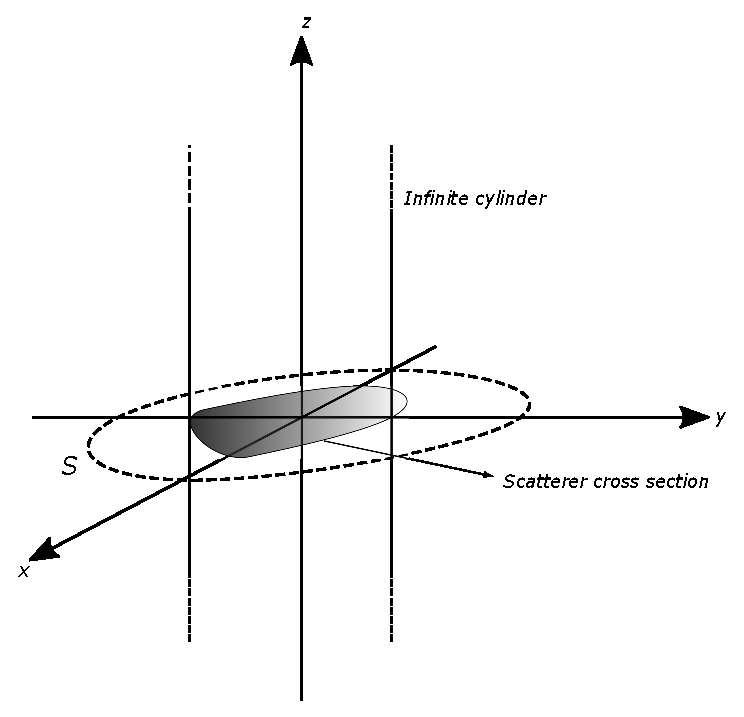
\includegraphics[width=0.4\textwidth]{./figuras/2dproblem}
				\caption{Infinite cylinder with inhomogeneous cross section.}
				\label{fig:2:2dproblem}
			\end{figure}
			\begin{eqnarray}
				E_{s_z}(\brho)\mathbf{z} &=& k_b^2 \int\limits_S\int_{-\infty}^{\infty}dz^\prime d\brhop\mathbf{\bar{G}}(\mathbf{r},\mathbf{r^\prime})\cdot\chi(\brhop)E_z(\brhop)\mathbf{z} \label{eq:2:2d:1} \\
				&=& k_b^2 \int\limits_S d\brhop \left[\int_{-\infty}^{\infty}dz^\prime\left(\mathbf{\bar{I}} + \frac{\nabla\nabla}{k_b^2}\right) \frac{-e^{jk_b|\mathbf{r}-\mathbf{r^\prime}|}}{4\pi|\mathbf{r}-\mathbf{r^\prime}|} \right]  \cdot\chi(\brhop)E_z(\brhop)\mathbf{z} \label{eq:2:2d:2}
			\end{eqnarray}
	
			%A integral em $z$ no lado direito da equação \eqref{eq:2:2d:2} tem resultado analítico conhecido \citep{balanis2012advanced}:
			The integral over $z$ on the right side of equation \eqref{eq:2:2d:2} is known \citep{balanis2012advanced}:
			\begin{equation}
				\int_{-\infty}^{\infty}dz^\prime\left(\mathbf{\bar{I}} + \frac{\nabla\nabla}{k_b^2}\right) \frac{e^{jk_b|\mathbf{r}-\mathbf{r^\prime}|}}{4\pi|\mathbf{r}-\mathbf{r^\prime}|}  = \frac{j}{4}H_0^{(2)}(k_b|\brho-\brhop|) \label{eq:2:2d:3}
			\end{equation}
		
			%\noindent onde $H_0^{(2)}$ é a função de Hankel de ordem zero e grau 2. Desta forma, \eqref{eq:2:2d:2} pode ser reescrita como:
			\noindent where $H_0^{(2)}$ is the Hankel function of the second kind. Thus, \eqref{eq:2:2d:2} can be rewritten as:
			\begin{equation}
				E_{s_z}(\brho) = -\frac{jk_b^2}{4} \int_S dS^\prime H_0^{(2)}(k_b|\brho-\brhop|) \chi(\brhop) E_z(\brhop)\label{eq:2:2d:4}
			\end{equation}
		
			%Similarmente, as equações \eqref{eq:2:waveequations:final}, \eqref{eq:2:eisp:5}, \eqref{eq:2:eisp:6} e \eqref{eq:2:eisp:9} podem ser reescritas como:
			Similarly, equations  \eqref{eq:2:waveequations:final}, \eqref{eq:2:eisp:5}, \eqref{eq:2:eisp:6}, and \eqref{eq:2:eisp:9} can be rewritten as:
			\begin{eqnarray}
				E_z(\brho) &=& E_{z_i}(\brho) - \frac{jk_b^2}{4} \int_S dS^\prime H_0^{(2)}(k_b|\brho-\brhop|) \chi(\brhop) E_z(\brhop) \label{eq:2:2d:5} \\
				E_{s_z}(\brho) &=& -\frac{jk_b^2}{4} \int_S dS^\prime H_0^{(2)}(k_b|\brho-\brhop|) J_{z_{eq}}(\brhop) \label{eq:2:2d:6} \\
				\chi(\brho)E_{z_i}(\brho) &=& J_{z_{eq}}(\brho) + \frac{jk_b^2}{4} \chi(\brho) \int_S dS^\prime H_0^{(2)}(k_b|\brho-\brhop|) J_{z_{eq}}(\brhop) \label{eq:2:2d:7} \\
				\beta(\brho)J_{z_{eq}}(\brho) &=& R(\brho)\beta(\brho)J_{z_{eq}}(\brho) \nonumber \\ && +~~ R(\brho)\left[ E_{z_i}(\brho) - \frac{jk_b^2}{4} \int_S dS^\prime H_0^{(2)}(k_b|\brho-\brhop|) J_{z_{eq}}(\brhop)\right] \label{eq:2:2d:8}
			\end{eqnarray}
		
			Recently, \cite{bevacqua2021effective} proposed to decompose the Hankel function in two terms using the known identity $H^{(2)}_0(x) = J_0(x) + Y_0$, where the $Y_0$ is the zero order Bessel function of second kind. Then, \eqref{eq:2:eisp:7} might be rewritten as:
			\begin{multline}
				\chi(\brho)E_{z_i}(\brho) = J_{z_{eq}}(\brho) + \frac{jk_b^2}{4} \chi(\brho) \int_S dS^\prime J_0(k_b|\brho-\brhop|) J_{z_{eq}}(\brhop) \\ + \frac{jk_b^2}{4} \chi(\brho) \int_S dS^\prime Y_0(k_b|\brho-\brhop|) J_{z_{eq}}(\brhop)  \label{eq:2:2d:greendecomp:csie}
			\end{multline}
		
			The first advantage in \eqref{eq:2:2d:greendecomp:csie} is that the first integral, which does not exhibit singularity, can be easily computed from the available scattered field data. Its meaning is the contribution of main spectral component of the radiating currents to the total field in $S$. The second advantage is the potential to mitigate the nonlinearity condition of the problem (see Subsection \ref{chap:problemstatement:eisp:4} for more information). The authors also provides a straightforward procedure to compute the first integral and a discretization formula to address the second integral.
		
		\subsection{Vector spaces and operator properties}\label{chap:problemstatement:eisp:3}
		
			%A função $\chi(\mathbf{r})$ é uma função contínua por partes, uma vez que representa as propriedades dielétricas dos meios no domínio. Desta forma, $\chi$ é uma função diferenciável e integrável exceto nas fronteiras dos meios. Já a função que representa o campo elétrico total, em problemas tridimensionais, pode apresentar descontinuidades em suas componentes devido à condições de interface entre os meios. No entanto, isso não acontece em problemas bidimensionais, uma vez que a componente $E_z$ é sempre perpendicular à normal definida na interface entre os meios. De qualquer maneira, essa grandeza é sempre integrável e diferenciável pelo menos no interior dos objetos. O mesmo vale para o campo espalhado. No entanto, ele é geralmente medido em meios homogêneos, ou seja, não costuma envolver discontinuidades.
			The $\chi(\mathbf{r})$ function is continuous by parts since it represents the dielectric properties of the media. Therefore, $\chi$ is an integrable and differentiable function except at the interface between media. The function which represents the total electric field, in three-dimensional problems, may have discontinuities in its components due to interface conditions. However, this does not happen in two-dimensional problems, since the $E_z$ component is always perpendicular to the normal defined on the interface between the media. Either way, the field is always integrable and differentiable. This is also true for the scattered field. However, it is generally measured in a homogeneous media, i.e., it does not usually involve discontinuities.
			
			%Levando em consideração a \eqref{eq:2:eisp:5}, o conjunto de todas campos espalhados pode ser definido em termos de um espaço linear de funções analíticas com crescimento exponencial no infinito e regular dentro de um subdomínio da região medição do campo $D$, o qual é exterior ao domínio do espalhador \citep{bucci1989degrees}. Essas funções são uniformemente limitadas nesse subdomínio uma vez que a corrente equivalente $\mathbf{J}_{eq}$ é uniformemente limitada. Em outras palavras, uma vez que o kernel de \eqref{eq:2:eisp:5} é analítico, este operador é compacto, e por isso, a imagem de qualquer conjunto limitado é pré-compacta \citep{bucci1989degrees}. Também é possível chegar às mesmas conclusões se, ao equiparmos os espaços de $\chi$ com a norma $L^{\infty}$ e o espaço de $\mathbf{E}$ com a norma $L^2$, assumirmos que o campo total dentro do espalhador é uniformemente limitado. Isto é coerente tendo em vista que o contraste e o campo incidente são limitados. Consequentemente, a corrente equivalente também pertence a um conjunto limitado e o campo espalhado pertence a um pré-compacto. Ademais, uma vez que o operador inverso de um compacto não pode ser contínuo, então o problema inverso é mal-posto.
			Taking into account \eqref{eq:2:eisp:5}, the set of all scattered fields can be defined in terms of a linear space of analytical functions with exponential growth at infinity and regular within a subdomain of the measurement region $D$, which is external to the scatterer domain \citep{bucci1989degrees}. These functions are uniformly bounded in this subdomain since the equivalent current $\mathbf{J}_{eq}$ is uniformly bounded. In other words, since the kernel of \eqref{eq:2:eisp:5} is analytical (except at singularities), this operator is compact, and therefore, the image of any bounded set is pre-compact \citep{bucci1989degrees}. It is also possible to reach the same conclusions if we assume that the total field within the scatterer is uniformly bounded, provided we equip the defined $\chi$ space with the $L^{\infty}$norm and the $\mathbf{E}$ space with the $L^2$ norm. This is consistent since the contrast and the incident field are limited. Consequently, the equivalent current also belongs to a bounded set and the scattered field belongs to a pre-compact one. Furthermore, since the inverse operator of a compact one cannot be continuous, then the inverse problem is ill-posed.
			
	%		%Portanto, podemos definir o espaço vetorial de funções de $\chi$ como um espaço de Hilbert $L^2(V)$ o qual é composto de funções que podem ser medidas e integráveis na definição de Lebesgue \citep{bartle1995elements}. No entanto, o espaço vetorial de  $\mathbf{E}(\mathbf{r})$ é mais restrito devido às equações de Maxwell \eqref{eq:2:maxwell:har:1}-\eqref{eq:2:maxwell:har:4}. Por isso, o espaço de $\mathbf{E}(\mathbf{r})$ e $\mathbf{E}_s(\mathbf{r})$ pode ser definido como um subconjunto $U\subset L^2(V)$.
	%		Thus, we can define the vector space of functions for $\chi$ as a Hilbert space $L^2(V)$ which is composed of functions that can be measured and integrable in the Lebesgue definition \citep{bartle1995elements}. However, the vector space of $\mathbf{E}(\mathbf{r})$ is more restricted due to Maxwell's equations \eqref{eq:2:maxwell:har:1}-\eqref{eq:2:maxwell:har:4}. Therefore, the space of $\mathbf{E}(\mathbf{r})$ and $\mathbf{E}_s(\mathbf{r})$ can be defined as a subset $U\subset L^2(V)$.
	%		
	%		%Se $\mathbf{E}$ fosse conhecido nas equações \eqref{eq:2:waveequations:final} e \eqref{eq:2:eisp:2}, os operadores $\mathcal{L}^D : L^2(V) \rightarrow U$ e $\mathcal{L}^S(V) : L^2 \rightarrow U$ seriam compactos e fracamente singulares, conforme o \autoref{the:app:functional:9}.
	%		If $\mathbf{E}$ were known in equations \eqref{eq:2:waveequations:final} and \eqref{eq:2:eisp:2}, the $\mathcal{L}^D : L^2(V) \rightarrow U$ and $\mathcal{L}^S(V) : L^2 \rightarrow U$ operators would be linear, compact, and weakly singular, according to \autoref{the:app:functional:9}.
		
		\subsection{Uniqueness, Stability and Nonlinearity}\label{chap:problemstatement:eisp:4}
			
			%Conforme discutido na \autoref{chap:problemstatement:inverse}, existem três critérios que precisam ser atendidos para que um problema seja considerado bem-posto. O problema inverso de espalhamento eletromagnético é mal-posto por não atender o critério de estabilidade. A condição de unicidade, embora garantida, é considerada apenas em análises teóricas do problema, i.e., em situações práticas, o problema não costuma ter solução única. Além disso, o problema é não-linear, o que confere outros aspectos ao problema.
			As discussed in Section \ref{chap:problemstatement:inverse}, three criteria need to be satisfied for a problem to be considered well-posed. EISP is ill-posed because it does not meet the stability criterion. The condition of uniqueness is considered only in some theoretical analyzes, i.e., in practical situations, the problem does not usually have a single solution. In addition, the problem is non-linear, which provides other aspects to the problem.
			
			%Uma vez que se trata de um problema físico com modelagem matemática coerente, a condição de existência de solução não é questionada. De um ponto de vista teórico, é mais importante questionar se o problema tem solução única. Conforme demonstrado por \cite{colton1992uniqueness}, a unicidade da permissividade relativa para um dado padrão de campo distante é garantida sob certas condições, dentre elas: um número fixo de número de onda, todas as direções de incidência e todas as polarizações do campo incidente. Todavia, em situações práticas, todas essas informações nem sempre estão disponíveis. Vale à pena destacar também que existem situações para as quais a unicidade não é garantida do ponto de vista analítico, como por exemplo, em problemas nos quais a permissividade e permeabilidade podem ser zero ou infinito.
			As demonstrated by \cite{colton1992uniqueness}, the uniqueness of the relative permittivity for a given distant field pattern is guaranteed under certain conditions, among them: a fixed number of wavenumber, all directions of incidence, and all polarizations of the field incident. Therefore, the existence condition is also fulfilled. However, in practical situations, all of this information is not always available. It is also worth noting that there are situations for which uniqueness is not guaranteed from an analytical point of view, such as, problems in which permittivity and permeability can be zero or infinite.
			
			%Mesmo que uma quantidade suficiente de informação esteja disponível para que o problema tenha solução única, a relação entre as variáveis conhecidas e desconhecidas não é contínua \citep{chen2017}. Conforme já foi demonstrado na literatura \citep{stefanov1990stability,caro2010stable}, para um problema envolvendo espalhadores dielétricos, se o erro nos dados conhecidos são no máximo $\delta$, então o pior cenário do erro na solução é da ordem de $\ln|\delta|^{-s}$, onde $0<s<1$. Isto é conhecido como uma estimativa de estabilidade do problema e, quando $\delta\rightarrow0$, pela regra de L'Hôpital, a ordem do erro aumenta drasticamente. Esse tipo de situação é conhecido na literatura como problema exponencialmente ou severamente mal-posto. Esse tipo de condição não pode ser mudada se tivermos infinitas medições de campo. No entanto, a estabilidade pode ser aumentada com algumas estratégias, como por exemplo, o aumento de frequências de operação \citep{bao2015inverse,nagayasu2013increasing,isakov2016increasing}.
			Even if a sufficient amount of information is available for uniqueness, the relationship between known and unknown variables is not continuous \citep{chen2017}. As already demonstrated in the literature \citep{stefanov1990stability,caro2010stable}, for a problem involving dielectric scatterers, if the error in the known data is at most $\delta$, then the worst scenario of the error in the solution is in the order of $\ln|\delta|^{-s}$, where $0<s<1$. This is known as a problem stability estimate and, when $\delta\rightarrow0$, by the L'Hôpital rule, the error order increases dramatically. This type of situation is known in the literature as an exponential or severely ill-posed problem. This type of condition cannot change if we have infinite field measurements. However, stability can increase with some strategies, such as, for example, increasing operating frequencies \citep{bao2015inverse,nagayasu2013increasing,isakov2016increasing}.
			
			%Conforme dito anteriormente, a relação entre contraste e campo espalhado não é linear uma vez que existem interações mútuas entre correntes induzidas. Por isso, o campo não pode ser interpretado como uma superposição linear de respostas individuais. Além disso, a não-linearidade do problema não é do tipo convexa, ou seja, do ponto de vista de otimização, podem haver múltiplos mínimos locais os quais podem fazer com que algoritmos fiquem presos em soluções falsas \citep{chen2017,bucci1997electromagnetic}. Por isso, encontrar a solução exata para o problema se torna mais complicado.
			As stated earlier, the relationship between contrast and scattered field is not linear since there are mutual interactions between induced currents. Therefore, we cannot interpret the field as a linear superposition of individual responses. Besides, the nonlinearity of the problem is not of the convex kind, i.e., from the optimization point of view, there may be multiple local minima which can cause algorithms to get trapped in false solutions \citep{chen2017,bucci1997electromagnetic}. Therefore, finding the exact solution becomes more complex. 
			
			A deeper explanation on non-linearity is found in \cite{bucci2001degree}. The authors developed the Degree of Nonlinearity (DNL) which is indicator to how difficult is solving the correspond EISP. Considering the state equation in the operator \eqref{eq:2:eisp:4}, the total field $E_z$ may be rewritten as:
			\begin{equation}
				\mathbf{E}_z(\mathbf{r}) = \left(\mathcal{I} - \mathcal{L}^S\{\chi(\mathbf{r})\}\right)^{-1} \mathbf{E}_i(\mathbf{r})
			\end{equation}
		
			\noindent where $\mathcal{I}$ is the identity operator and $$\mathcal{L}^S\{\chi(\mathbf{r})\} = - k_b^2\int_V d\mathbf{r^\prime} \mathbf{\bar{G}}(\mathbf{r},\mathbf{r^\prime})\cdot\chi(\mathbf{r^\prime}).$$
			
			When the $L^2$-norm over $ \mathcal{L}^S\{\chi(\mathbf{r})\}$ is lower than 1, the inverse operator is approximated by Neumann series, i.e.:
			\begin{equation}
				\left(\mathcal{I} - \mathcal{L}^S\{\chi(\mathbf{r})\}\right)^{-1} = \mathcal{I} + \mathcal{L}^S\{\chi(\mathbf{r})\} + \left(\mathcal{L}^S\{\chi(\mathbf{r})\}\right)^2 + \cdots + \left(\mathcal{L}^S\{\chi(\mathbf{r})\}\right)^n + \cdots
			\end{equation}
			
			Then, \cite{bucci2001degree} defined DNL indicator as $||\mathcal{L}^S\{\chi(\mathbf{r})\}||_{L^2}$. They observed that, the smaller than 1 DNL is, the stronger linear approximation is. As DNL tends to 1, a polynomial relation holds true between data and unknowns. The larger the order of polynomial is, the larger the number of local minima. When DNL is greater than 1, then a non-polynomial relation holds true. Therefore, the larger the DNL, the larger overall difficulty of the problem due its nonlinearity. In these cases, the possible number of local minima in respect to some cost functional can be higher, which increases the difficulty of finding the global minimum that defines the solution of the inverse problem. Moreover, the indicator is also applied to the two-dimensional case \eqref{eq:2:2d:5}, the Contrast Source Integral Equation \eqref{eq:2:2d:7}, its Extended-Born version \eqref{eq:2:2d:8}, and when the Green's function is decomposed \citep{durso2010solution,bevacqua2021effective}. In \cite{durso2010solution}, the authors provide criteria for choosing between \eqref{eq:2:2d:7} and \eqref{eq:2:2d:8}. In \cite{bevacqua2021effective}, the authors show that the Green's Function Decomposition formulation has a much lower growth of DNL than the traditional Contrast Source Integral \eqref{eq:2:2d:7} when the scatterer size increases. \cite{bevacqua2021quantitative} showed that, for certain configurations of scatterers and values of $\beta$ in \eqref{eq:2:eisp:9}, the DNL can be drastically reduced (mainly when $\beta\ge2$). The authors also showed significant reductions in the degree of non-linearity when the Y0 \eqref{eq:2:2d:greendecomp:csie} and NIE \eqref{eq:2:eisp:9} formulations are combined \citep{bevacqua2021new}. For $\beta=6$, the results showed less DNL growth as the scatterer grew when compared to the other formulations.
			
			%Os autores mostraram que, para determinadas configurações de espalhadores e valores de $\beta$ em \eqref{eq:2:eisp:9}, o DNL pode ser reduzido drasticamente (principalmente quando $\beta\ge2$). Os autores também mostraram significativas reduções do grau de não-linearidade quando a formulações Y0 \eqref{eq:2:2d:greendecomp:csie} e NIE \eqref{eq:2:eisp:9} são combinadas. Para $\beta=6$, os resutados mostraram um crescimento menor do DNL conforme o espalhador crescia em comparação com as outras formulações.
			
		\subsection{Degrees of Freedom}\label{chap:problemstatement:eisp:5}
	
			%Do ponto de vista analítico, dois campos são distinguíveis quando suas definições são distintas entre si. No entanto, quando essas grandezas físicas diferem muito pouco entre si, elas podem ser indistinguíveis na prática. Existem muitos fatores que podem contribuir para a impossibilidade de destinguir campos, como por exemplo, ruídos, dinâmicas dos mecanismos de medição, precisão e erros numérios. Baseado na definição do conceito de distinção é que é possível definir diferentes estados do sistemas, e com isso, a noção de um número mínimo de parâmetros independentes que podem descrever o sistema até uma certa precisão. Este assunto tem um papel importante em EISPs uma vez que campos espalhados que sejam considerados indistinguíveis vão ter reconstruções idênticas as quais nem sempre vão representar bem os meios investigados.
			From an analytical point of view, two fields are distinguishable when their definitions are distinct from each other. However, when these physical quantities differ very little from each other, they can be indistinguishable in practice. Many factors can contribute to the impossibility of distinguishing fields, such as, for example, noise, dynamics of measurement mechanisms, precision, and numerical errors. Based on the definition of the concept of distinction, it is possible to define different states of the system, and with that, the notion of a minimum number of independent parameters that can describe the system to a certain precision. This issue plays an important role in EISPs since scattered fields that are considered indistinguishable will have identical reconstructions which will not always represent the investigated media well.
			
			%No primeiro trabalho sobre o tema, \cite{bucci1989degrees} mostraram que o número de graus de liberdade de um campo espalhado é essencialmente igual ao número de Nyquist definido proporcionalmente às dimensões das regiões de fonte e de observação. Particularmente, o número de Nyquist $N_0$ foi definido como:
			In the first work on the subject, \cite{bucci1989degrees} showed that the number of Degrees of Freedom (DoF) in a scattered field is essentially equal to the Nyquist number defined in proportion to the dimensions of the source and observation regions. In particular, the Nyquist $N_0$ number was defined as:
			\begin{equation}
				N_0 = \frac{2SW_0}{\pi} \approx \frac{2Ska}{\pi} \label{eq:2:dof:1}
			\end{equation}
		
			%\noindent onde $S$ é a metade do comprimento do domínio de observação, $W_0$ é a largura de banda do sinal, $k_b$ é o número de onda do meio de fundo e $a$ é o raio máximo do domínio que os espalhadores ocupam. Este, então, seria o número mínimo de parâmetros (informação) necessário para representar com uma certa precisão o campo espalhado. Os autores também concluíram uma interpolação amostral em pontos equidistantes seria uma reconstrução praticamente ótima do campo espalhado.
			\noindent where $S$ is half the length of the observation domain, $W_0$ is the signal bandwidth, $k$ is the source wavenumber  and $a$ is the maximum radius of the domain that the scatterers occupy. This, then, would be the minimum number of parameters (information) necessary to represent the spread field with a certain precision. The authors also concluded that a sample interpolation at equidistant points would be a practically optimal reconstruction of the scattered field.
			
			%Posteriormente, \cite{bucci1997electromagnetic}, baseados no fato de que apenas representação de dimensão finita do contraste pode ser reconstruída, avaliaram qual a dimensão do espaço de dados coerente com uma certa configuração do espaço que representa o contraste. Esta avaliação foi feita tanto para um caso de única indicidência como múltiplas. No caso de incidência simples, os autores perceberam que a relação entre quantidade e valor de autovalores do kernel em \eqref{eq:2:eisp:5} tem um comportamento semelhante à função degrau, i.e., a medida que a quantidade de autovalores cresce, seus valores sofrem uma queda brusca a partir de um certo limiar. Além disso, quando maior o espalhador, mais brusca a queda. Esse comportamento também em relação ao erro de aproximação, o que significa dizer que o número dos graus de liberdade pode ser identificado uma quantidade de autovalores para o qual o erro de aproximação ultrapassa um certo limiar estabelecido. Para o caso de fontes esféricas e superfícies de observação esféricas e concêntricas, se $k_ba \gg 1$, então o número de graus de liberdade $M$ será:
			Subsequently, \cite{bucci1997electromagnetic} evaluated the dimension of the data space which is consistent with a certain contrast space configuration. Their analysis is based on the fact that only a finite-dimensional representation of the contrast can be reconstructed. This assessment was made for both single and multiple cases. In the case of simple incidence, the authors realized that the relationship between amount and value of kernel eigenvalues in \eqref{eq:2:eisp:5} behaves similarly to the step function, i.e., as the number of eigenvalues grows, their values fall sharply from a certain threshold. Also, the larger the scatterer, the more sudden the fall. This behavior is also observed when we consider the approximation error, which allows us to identify the number of degrees of freedom by the number of eigenvalues for which the approximation error exceeds a certain established threshold. For spherical sources and spherical (concentric) observation surfaces, if $k_ba \gg 1$, then DoF is approximated by:
			\begin{equation}
				DoF \approx (ka)^2 \label{eq:2:dof:2}
			\end{equation}
		
			%Num caso bidimensional de círculos concêntricos para fontes circulares:
			In a two-dimensional case of concentric circles for circular sources:
			\begin{equation}
				DoF \approx 2ka \label{eq:2:dof:3}
			\end{equation}
		
			%Já no caso da incidência múltipla, os autores afirmaram que o número de parâmetros independentes não pode ser maior que $M^2/2$, onde $M$ é o número de graus de liberdade para incidência simples. Em seus experimentos, os autores não visualizaram diferença significativa entre uma amostragem $32\times32$ e uma $36\times36$ no caso de um objeto circular de baixo contraste com diâmetro $5\lambda_b$ ($M\approx32$).
			Considering multiple incidences, the authors stated that the number of independent parameters must not be greater than $DoF^2/2$, where $DoF$ is the number of degrees of freedom for simple incidence. In their experiments, the authors did not observe a significant difference between a $32\times32$ and a $36\times36$ scattered matrices, considering a low contrast circular object with a diameter of $5\lambda_b$ ($DoF\approx32$).
			
			 \cite{chew1994inverse} also discussed this issue. Firstly, they demonstrated why solving \eqref{eq:2:eisp:5} for $\mathbf{J}_{eq}$ and evaluating $\mathbf{E}$ and $\chi$ through \eqref{eq:2:waveequations:final} and $\mathbf{J}_{eq}/\mathbf{E}$, respectively, is not an adequate approach. Although it seems attractive since there is no iteration process, the solution in practical situations is not unique, as discussed in Subsection \ref{chap:problemstatement:eisp:4}. One of the solutions is due to non-radiating sources which are also inverse solutions to the Green's function. The non-radiating solution is due to the non-trivial null space in \eqref{eq:2:eisp:5}, i.e., there is a non-trivial solution for $\mathbf{E}_s=\mathbf{0}$. Consequently, if a unique solution to \eqref{eq:2:eisp:5} is obtained (e.g., minimum norm solution through pseudo-inverse method \citep{ney1984solution}), the null space solution is eliminated. Even though, it does not contribute to the scattered field, it does contribute to the total field within the scatterer. Therefore, without the null space solution, the total field obtained by the application of $\chi\mathbf{E}=\mathbf{J}_{eq}$ in \eqref{eq:2:waveequations:final} and the following contrast function estimation by $\mathbf{J}_{eq}/\mathbf{E}$ will not be correct.
			
			Second, the authors stated that a very large number of measurements will not make the null space smaller, which agrees with \cite{bucci1989degrees} and  \cite{bucci1997electromagnetic}. In addition, the difference in the dimensionality between the measurement and image domains is also a practical obstacle for raising the number of measurements. The authors called the growth of linear dependency as the number of measurements increases as the \textit{law of diminishing return}. Their explanation is based on the high-spatial-components of the induced current which generates evanescent waves that decay fast away from the scatterer and are very small at the measurement space. The decay is also related to the nature of the Green's function which can be compared to a low-pass filter. These components also contributes to the null space. Through the Fourier analysis of the scattered field, the authors came to the same conclusion as \cite{bucci1989degrees} about the Nyquist number as upper bound of sampling rate.
			
			Finally, some efforts have been made towards a numerical approach for computing DoF. \cite{lin2021study} proposed to modify the Green function taking into account the maximum contrast value and evaluate DoF based on the singular values of the Green function. When the maximum contrast is not available, then it is assumed that the contrast tends to infinity and a new modification for the Green function is formulated. 
		
	\section{Conclusion}
	
		%Este capítulo apresentou uma breve discussão sobre os aspectos teóricos do problema inverso de espalhamento eletromagnético. A seção 1 introduziu as grandezas e suas relações mais básicas levando em consideração um modelo com meios lineares, isotrópicos, não-dispersivos e não-magnéticos. A seção 2 apresentou o desenvolvimento da equação integral \eqref{eq:2:waveequations:final} que é a base para o problema. Baseado na definição proposta por \cite{hadamard1923lectures}, a seção 3 discutiu o que é um problema inverso mal-posto através dos critérios de existência, unicidade e estabilidade de solução. Além disso, a seção também apresentou a formulação geral de operadores de regularização através da equação \eqref{eq:2:inverse:2}. A seção 4 definiu o problema inverso de espalhamento eletromagnético apresentando as formulações tridimensionais através das equações \eqref{eq:2:eisp:2}, \eqref{eq:2:eisp:5}-\eqref{eq:2:eisp:9}; e as formulações bidimensionais baseadas no Modo Transversal Magnético em $z$ descritas nas equações \eqref{eq:2:2d:4}-\eqref{eq:2:2d:8}. Além disso, foram discutidas as propriedades dos espaços vetorais e operadores envolvidos no problema. Também foi demonstrado que o problema pode ter solução única em algumas situações que dificilmente são possíveis na prática. De qualquer maneira, até quando existe solução única, o problema é mal-posto por questões de instabilidade cuja a explicação pode ser demonstrada através da teoria de operadores inversos de operadores compactos. Ademais, a instabilidade pode ser quantificada através da estimativa de pior-caso a qual é exponencial para o problema. Além destes fatores que dificultam a solução do problema, a não-linearidade do tipo não-convexo é uma característica importante a qual pode fazer com que algoritmos de otimização fiquem presos em mínimos locais que representam imagens espúrias. Por fim, os graus de liberdade do problema foram definidos através da \eqref{eq:2:dof:3} o qual é uma medida importante para a determinação da quantidade necessária de observações do campo espalhado considerando uma determinada configuração do problema.
		This chapter presented a brief discussion of the theoretical aspects of EISP. Section \ref{chap:problemstatement:eletromagnetic} introduced the physical quantities and their most basic relations taking into account a model with linear, isotropic, non-dispersive, and non-magnetic materials. Section \ref{chap:problemstatement:integral} presented the development of the integral equation \eqref{eq:2:waveequations:final} that is the basis for the problem.
		
		Based on the definition proposed by \cite{hadamard1923lectures}, Section \ref{chap:problemstatement:inverse} discussed what is an an ill-posed inverse problem through the criteria of existence, uniqueness, and stability of the solution. The section also presented the general formulation of regularization operators using equation \eqref{eq:2:inverse:2}.
		
		Section \ref{chap:problemstatement:eisp} defined the electromagnetic inverse scattering problem by presenting three-dimensional formulations through equations \eqref{eq:2:eisp:2}, \eqref{eq:2:eisp:5}-\eqref{eq:2:eisp:9}; and the two-dimensional formulations based on the TMz mode described through equations \eqref{eq:2:2d:4}-\eqref{eq:2:2d:8}. Besides, the properties of the vector spaces and operators were discussed. It has also been shown that the problem can have a unique solution in some situations which are hardly possible in practice. Nevertheless, even when there is a unique solution, the problem is still ill-posed for reasons of instability whose explanation can be demonstrated through the theory of inverse operators of compact ones. Furthermore, instability can be quantified through the worst-case estimate which is exponential for the problem. In addition to these factors that contribute to the complexness of the problem, non-convex non-linearity is an important feature that can cause optimization algorithms to be trapped in local minima which may represent spurious images. Finally, the degrees of freedom of the problem were defined using \eqref{eq:2:dof:3}, which is an important measure for determining the necessary amount of observations of the scattered field considering a given configuration of the problem.
		
    % ------------------------------------------------------------------------------
% Methods Overview
% ------------------------------------------------------------------------------

\chapter{Methods Overview}\label{chap:methods}

	%Uma vez que expressões analíticas para o problema só são possíveis em algumas situações onde a geometria do problema é bem delimitada, é necessário utilizar abordagens numéricas para resolver o problema inverso. Este capítulo tem o objetivo de fazer uma ampla revisão cobrindo tanto as formas de discretização, necessárias para a implementação computacional, como para as formas de se obter uma solução.
	%Since analytical expressions for the problem are only possible in some situations where the problem geometry has a simple shape, it is necessary to use numerical approaches to solve the inverse problem. This chapter has the objective of carrying out a wide-ranging review covering both forms of discretization (necessary for the computational implementation) and the ways to obtain a solution.
	
	%Primeiro, será apresentado um esquema geral do problema a partir de definição bem comum do domínio do problema. Na sequência, serão discutidas as diversas abordagens de discretização das equações para o problema bidimensional. As metodologias para abordagem linear para o problema são apresentadas em seguida. Embora essa dissertação tenha como objetivo o problema não-linear, muitos métodos adotam a versão linearizada tanto para inicializações como pequenos passos na busca. A duas classes de métodos quantitativos são apresentadas e discutidas na sequência, i.e., os métodos determinísticos e os estocásticos. A proposta destas duas seções é fazer uma revisão bibliográfica, elencando os principais métodos, estratégias e ideias propostas na literatura. Além dessas classes, foi dado destaque também a aplicação de métodos Deep-Learning que tem recebido muita atenção na literatura recentemente. Por fim, uma breve conclusão destacando os principais pontos do capítulo é apresentada.
	%First, a general outline of the problem will be presented in Section \ref{chap:methods:definition} from a standard definition of the problem domain. Following, in Section \ref{chap:methods:discretization}, the various approaches to discretization of the equations for the two-dimensional problem will be discussed. The methodologies for a linear approach to the problem are presented in Section \ref{chap:methods:linear}. Regularization methods are also used after linearization of the integral equation and are presented in Section \ref{chap:methods:regularization}. Section \ref{chap:methods:qualitative} presents methods for cases when only the shape of the scatterers are necessary to recover, i.e., qualitative methods. On the other hand, the two classes of quantitative methods are presented and discussed in the sequence, i.e., the deterministic (Section \ref{chap:methods:deterministic}) and stochastic ones (Section \ref{chap:methods:stochastic}). The purpose of these two sections is to present a bibliographic review, listing the main methods, strategies and ideas proposed in the literature. In addition to these classes, emphasis was also placed on applying Deep-Learning methods (Section \ref{chap:methods:deep}), which has recently received much attention in the literature. Lastly, a brief conclusion highlighting the main points of the chapter is presented in Section \ref{chap:methods:conclusion}.
	
	Since the inverse problem is ill-posed and nonlinear, analytical approaches are usually not considered. Due to such complexity numerical approaches are necessary to obtain a solution. This chapter aims to provide a comprehensive review of the various methods and techniques used to address the inverse problem.
	
	Section \ref{chap:methods:definition} presents a general overview of the problem domain, followed by a discussion on the different approaches to discretization of the equations for the two-dimensional problem in Section \ref{chap:methods:discretization}. In Section \ref{chap:methods:linear}, methodologies for a linear approach to the problem are presented. Regularization methods, which are used after linearization of the integral equation, are discussed in Section \ref{chap:methods:regularization}.
	
	Section \ref{chap:methods:qualitative} focuses on qualitative methods, which are used when only the shape of the scatterers needs to be recovered. The two classes of quantitative methods are presented in the subsequent sections, i.e., deterministic methods in Section \ref{chap:methods:deterministic} and stochastic methods in Section \ref{chap:methods:stochastic}. These sections provide a bibliographic review of the main methods, strategies, and ideas proposed in the literature.
	
	The chapter also emphasizes the application of Deep-Learning methods, which has recently gained significant attention in the literature, as discussed in Section \ref{chap:methods:deep}. Lastly, a brief conclusion is presented in Section \ref{chap:methods:conclusion} to summarize the main points covered in the chapter.
	

	\section{Domain Definition}\label{chap:methods:definition}
	
	 	%Toda a investigação conduzida neste trabalho pressuporá um problema bidimensional TMz com materiais lineares, isotrópicos, não-dispersivos e não-magnéticos. Portanto, \eqref{eq:2:2d:4}-\eqref{eq:2:2d:8} serão as equações que descreverão as relações entre campos, fonte e meio. No entanto, antes de adentrar nas metodologias, é necessário definir adequadamente o domínio do problema, i.e., a geometria dos espaços onde serão definidas todas as variáveis e constantes. Essas definições serão o referencial de todas as metodologias descritas nesse trabalho.
	 	All the research conducted in this work will presuppose a two-dimensional TMz problem with linear, isotropic, non-dispersive and non-magnetic materials. Therefore, \eqref{eq:2:2d:4}-\eqref{eq:2:2d:8} will be the equations that will describe the relationships between fields, source and medium. However, before entering the methodologies, it is necessary to adequately define the problem domain, i.e., the geometry of the spaces where all variables and constants are defined. These definitions will be the foundation for all the methodologies described in this work.
	 	
	 	%A Figura \ref{fig:3:domaindefinition} descreve a geometria do problema. O campo espalhado $E_{z_s}$ é definido sobre um círculo centrado na origem dos eixos cartesianos cujo raio é denotado por $R_O$, e o ângulo, por $\theta$. Esse círculo está imerso em um meio homogêneo caracterizado pelas propriedades eletromagnéticas $\epsilon_b$, $\sigma_b$ e $\mu_b$. O vetor $\brho$ em \eqref{eq:2:2d:4}-\eqref{eq:2:2d:8} pode ser escrito como:
	 	\autoref{fig:3:domaindefinition} describes the geometry of the problem. The scattered field $E_{z_s}$ is defined over a circle centred on the origin of the Cartesian axes whose radius is denoted by $R_O$, and the angle, by $\theta$. This circle is immersed in a homogeneous medium characterized by the electromagnetic properties $\epsilon_b$, $\sigma_b$, and $\mu_b$. The vector $\brho$ in \eqref{eq:2:2d:4}-\eqref{eq:2:2d:8} can be written as:
	 	\begin{equation}
	 		\brho = R_O\cos\theta\mathbf{x} + R_O\sin\theta\mathbf{y} \label{eq:3:definition:1}
	 	\end{equation}
		\begin{figure}[!b]
			\centering
			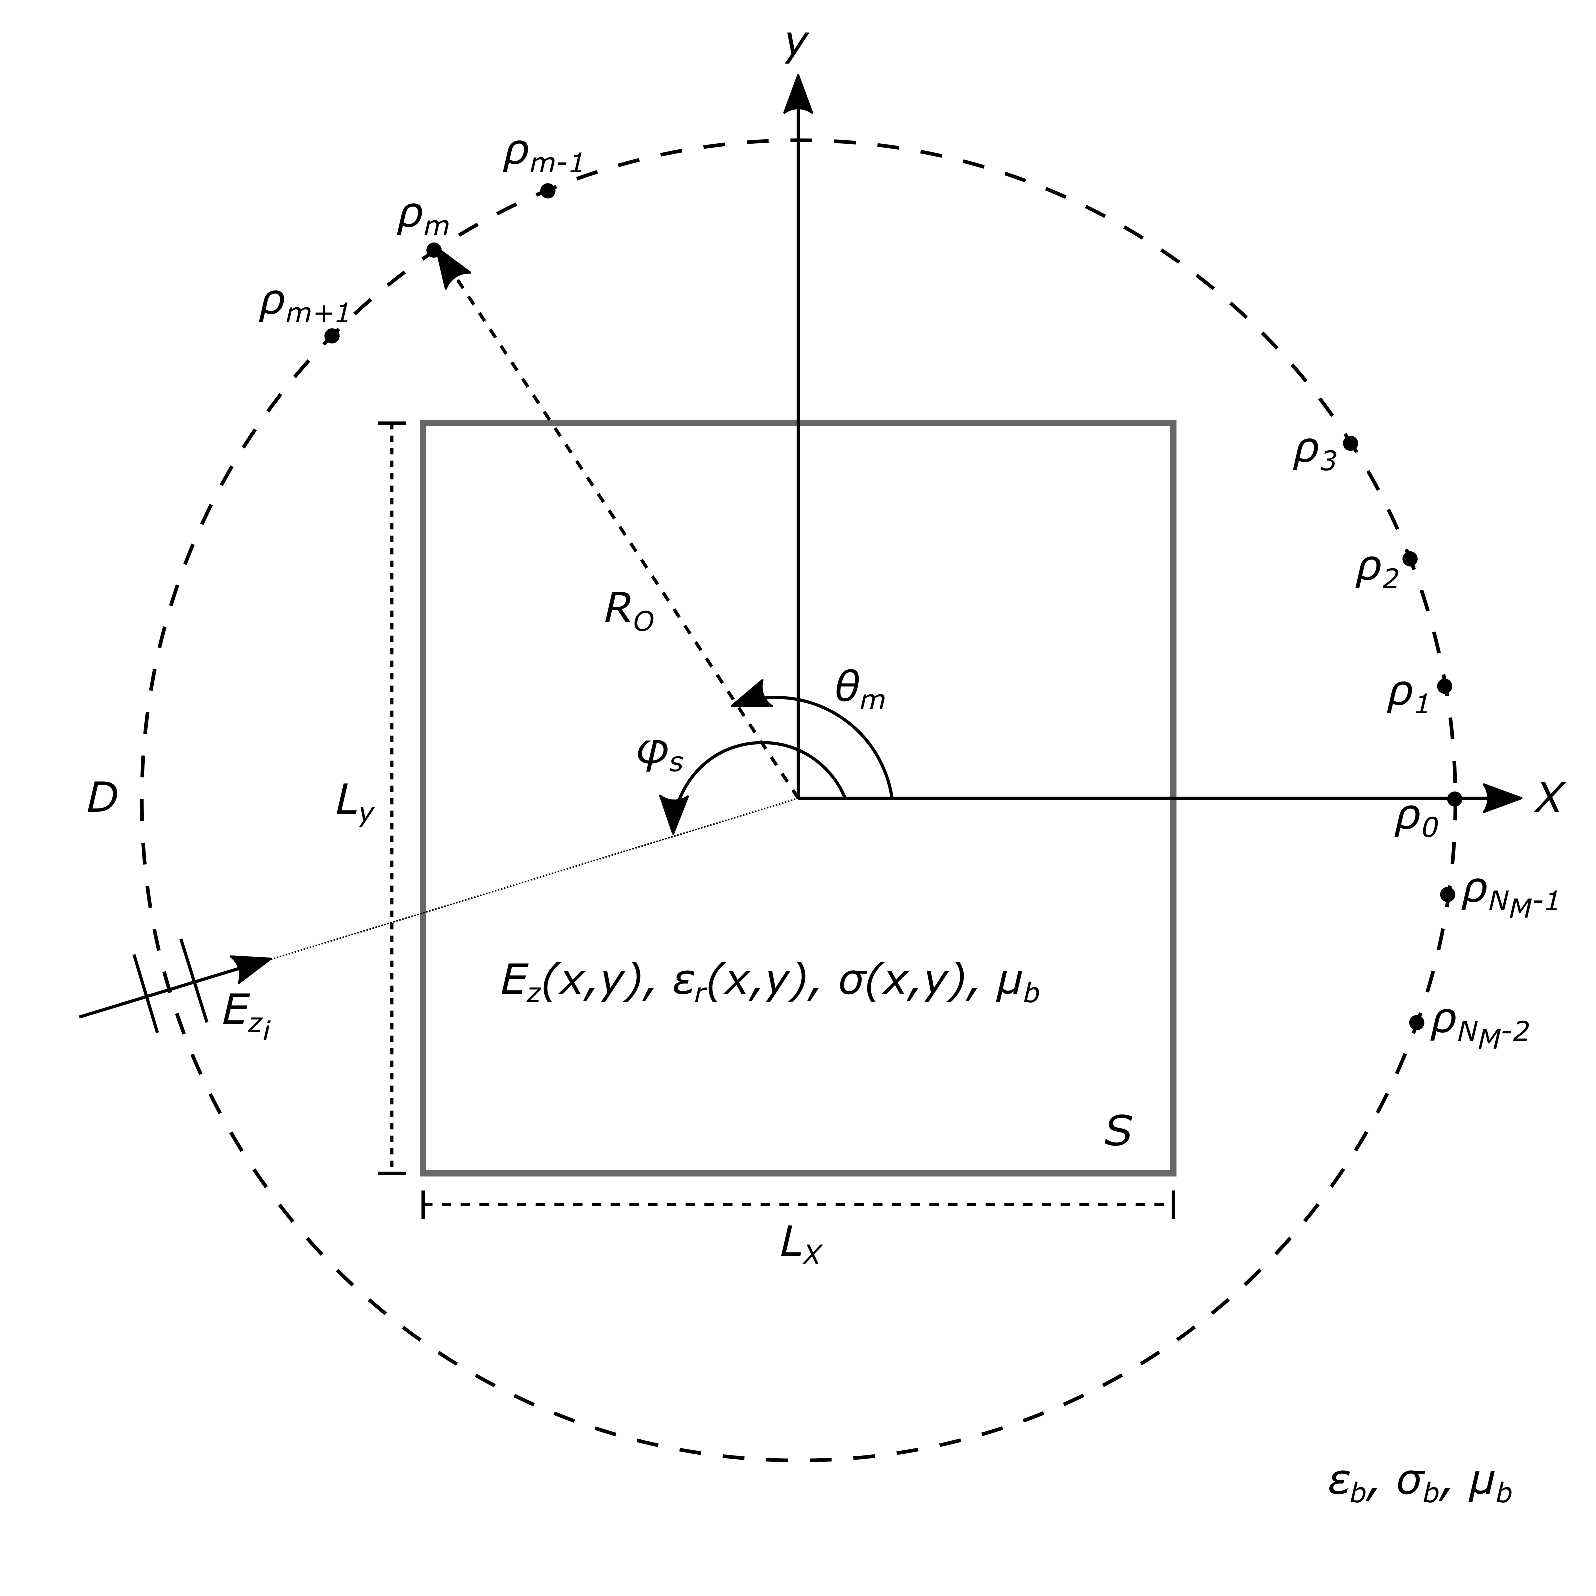
\includegraphics[width=0.5\textwidth]{./figuras/domaindefinition}
			\caption{Problem geometry.}
			\label{fig:3:domaindefinition}
		\end{figure}
 	
 		%O espaço de estados $S$ é a região retangular centrada na origem no eixo de coordenadas cujos comprimentos equivalem a $L_X$ e $L_Y$. Esta região representa a imagem a ser reconstruída, por isso, são definidas dentro delas as variáveis $E_z$, $\epsilon_r$ e $\sigma$. As duas últimas estão relacionadas à função contraste $\chi$ através de \eqref{eq:2:contrast}.
 		The state-space $S$ is the rectangular region centred at the origin on the axis of coordinate whose lengths are equal to $L_X$ and $L_Y$. This region represents the image to be reconstructed. Therefore, the variables $E_z$, $\epsilon_r$, and $\sigma$ are defined within them. The last two are related to the contrast function $\chi$ through \eqref{eq:2:contrast}.
 		
 		%Por fim, o campo incidente $E_{i_z}$ será representado por uma onda plana a qual é conhecida em todo o espaço do problema. A amplitude desta onda será denotada por $E_0$ enquanto seu ângulo de incidência em relação ao eixo cartesiano será denotado por $\phi$. Portanto, o campo incidente pode ser escrito como:
 		Finally, the incident field $E_{i_z}$ will be represented by a plane wave known throughout the problem space. The amplitude of this wave will be denoted by $E_0$, while its incidence angle concerning the Cartesian axis will be denoted by $\phi$. Therefore, the incident field can be written as:
 		\begin{equation}
 			E_{i_z}(\brho) = E_0e^{-j\mathbf{k_b}\cdot\brho} \label{eq:3:definition:2}
 		\end{equation}
 	
 		%\noindent no qual $\mathbf{k_b} = |k_b|\cos\phi\mathbf{x} + |k_b|\sin\phi\mathbf{y}$ é o vetor de número de onda. Outras formas de ondas incidentes são possíveis e toda a metodologia descrita e investigada no restante do texto é compatível.
 		\noindent where $\mathbf{k_b} = |k_b|\cos\phi\mathbf{x} + |k_b|\sin\phi\mathbf{y}$ is the wavenumber vector. Other forms of incident waves are possible and compatible with the methodology described throughout this chapter.
 		
 		%O espaço de dados $D$ será definido um domínio bidimensional conforme a seguir:
 		Data-space $D$ will be defined as a two-dimensional domain as follows:
 		\begin{equation}
 			D \coloneqq \{(\theta,\phi) : \theta, \phi \in [0,2\pi] \} \label{eq:3:definition:3}
 		\end{equation}
 	
 		%Ou seja, $D$ é uma região que relaciona os ângulos no qual o campo espalhado é definido e os de incidência. Obviamente, o campo espalhado não somente varia conforme $\theta$, mas também conforme o ângulo de incidência, uma vez que o campo espalhado é resultante da interação do campo incidente com o objeto espalhador. Por isso, a partir de agora, diremos que $E_{z_s}$ é uma função definida no domínio $D$, i.e., $E_{z_s}(\theta,\phi)$. Este tipo de definição também seria possível com ondas incidentes produzidas fontes impressas pontuais num arranjo circular, por exemplo.
 		Therefore, $D$ is a region that relates the angles in which the scattered field is defined and those of incidence. The scattered field varies according to $\theta$ and according to the angle of incidence ($\phi$) since the field scattered is the result of the interaction of the incident field with the scattering object. So, from now on, we will say that $E_{z_s}$ is a function defined in the $D$ domain, i.e., $E_{z_s}(\theta,\phi)$. This definition would also be possible with incident waves due to infinitesimal impressed sources in a circular arrangement.
 		
 		%A partir dessas definições, \eqref{eq:2:2d:4}-\eqref{eq:2:2d:8} serão reescritas como:
 		From those definitions, \eqref{eq:2:2d:4}-\eqref{eq:2:2d:8} will be rewritten as:
 		\begin{eqnarray}
 			E_{s_z}(\theta,\phi) &=& -\frac{jk_b^2}{4} \int_S dx dy~ G^D_{2D}(\theta,x,y) \chi(x,y) E_z(\phi,x,y)\label{eq:3:definition:4} \\[5pt]
 			E_z(\phi,x,y) &=& E_{z_i}(\phi,x,y) \nonumber \\[5pt]
 			&& ~~~~ - \frac{jk_b^2}{4} \int_S dx^\prime dy^\prime~ G^S_{2D}(x,y,x^\prime,y^\prime) \chi(x^\prime,y^\prime) E_z(\phi,x^\prime,y^\prime) \label{eq:3:definition:5} \\[5pt]
 			E_{s_z}(\theta,\phi) &=& -\frac{jk_b^2}{4} \int_S dxdy~ G^D_{2D}(\theta,x,y) J_{z_{eq}}(\phi,x,y) \label{eq:3:definition:6} \\[5pt]
 			\chi(x,y)E_{z_i}(\phi,x,y) &=& J_{z_{eq}}(\phi,x,y) \nonumber \\[5pt]
 			&& ~~~~~~~ + \frac{jk_b^2}{4} \chi(x,y) \int_S dx^\prime dy^\prime G^S_{2D}(x,y,x^\prime,y^\prime) J_{z_{eq}}(\phi,x,y) \label{eq:3:definition:7} \\[5pt]
 			\beta(x,y)J_{z_{eq}}(\phi,x,y) &=& R(x,y)\beta(x,y)J_{z_{eq}}(\phi,x,y) + R(x,y)\bigg[ E_{z_i}(\phi,x,y) \nonumber \\[5pt]
 			&& \left. ~~~~~~~~~~~~~ - \frac{jk_b^2}{4} \int_S dx^\prime dy^\prime~ G^S_{2D}(x,y,x^\prime,y^\prime) J_{z_{eq}}(\phi,x^\prime,y^\prime)\right] \label{eq:3:definition:8}
 		\end{eqnarray}
 	
 		%\noindent where\footnote{O leitor deve ter notado que, diferentemente de outros trabalhos na literatura \citep{chen2017}, aqui utilizaremos a letra $D$ para a região do campo espalhado e a letra $S$ para a região da imagem. Esta escolha foi feita para que o sobrescrito de $G_{2D}$ indique se a equação é a dados ou de estados.}:
 		\noindent where\footnote{The reader should have noticed that, unlike other works in the literature \citep{chen2017}, we will use the letter $D$ for the region of the scattered field and the letter $S$ for the image region. It is a choice made so that the $G_{2D}$ superscript indicates whether the equation is data or state.}
 		\begin{eqnarray}
 			G^D_{2D}(\theta,x,y) &=&  H_0^{(2)}(k_b\sqrt{(R_O\cos\theta-x)^2+(R_O\sin\theta-y)^2}) \label{eq:3:definition:9} \\[5pt]
 			G^S_{2D}(x,y,x^\prime,y^\prime) &=&  H_0^{(2)}(k_b\sqrt{(x-x^\prime)^2+(y-y^\prime)^2}) \label{eq:3:definition:10}
 		\end{eqnarray}
 	
 		The choice for such geometry is to be as simple as possible since the intention is to avoid any influence that any specific characteristic can perform. The advantage is that it is simpler for the definition of classical discretization formulas. On the other hand, it may not represent most of the real problems. However, this is not the goal of the thesis.
 	
 	\section{Discretization}\label{chap:methods:discretization}
 	
 		%Em situações práticas, o campo espalhado $E_{z_s}$ é conhecido somente em um conjunto de pontos em $D$. Além disso, para que \eqref{eq:3:definition:4}-\eqref{eq:3:definition:8} sejam resolvidas numericamente, é necessário adotar algum tipo de discretização. No contexto de métodos numéricos para equações diferenciais, a discretização é feita a partir da definição da forma fraca e forte das equações \citep{liu2009meshfree}. Um exemplo de metodologia baseado na forma forte é o Método das Diferenças Finitas onde as derivadas são aproximadas por diferenças entre valores nodais finitos \citep{taflove2005computational}. Já em relação à forma fraca, existe uma classe de métodos baseados no ponderamento dos resíduos das equações. É o chamado Método dos Resíduos Ponderados (MWR) \citep{fletcher1984computational}. Nestes métodos, para uma dada equação diferencial:
 		In practical situations, the scattered field $E_{z_s}$ is known only at a set of points in $D$. Furthermore, it is necessary to adopt some discretization to solve \eqref{eq:3:definition:4}-\eqref{eq:3:definition:8} numerically. In the context of numerical methods for differential equations, the discretization is made either from the weak or from the strong forms of the equations \citep{liu2009meshfree}. An example of a methodology based on the strong form is the Finite Difference Method, where the derivatives are approximated by differences between finite nodal values \citep{yee1966numerical,taflove2005computational}. Regarding the weak one, there is a class of methods based on weighting the residuals of the equations. It is called the Method of Weighted Residuals (MWR) \citep{fletcher1984computational}. In these methods, for a given differential equation:
 		\begin{equation}
 			\mathcal{K}\{u\} = 0 \label{eq:3:discretization:0}
 		\end{equation}
 	
 		%\noindent a solução aproximada $u_a$ é escrita da seguinte forma:
 		\noindent the approximate solution $u_a$ is written as follows:
 		\begin{equation}
 			u_a(\mathbf{r}) = u_0(\mathbf{r}) + \sum\limits_{j=1}^N a_j\psi_j(\mathbf{r}) \label{eq:3:discretization:1}
 		\end{equation}
 	
 		%\noindent onde $u_0$ é uma função que atenda as condições de contorno, $a_j$ são constantes desconhecidas e $\psi$ são funções analíticas geralmente chamadas de funções de tentativa. A função resíduo $R_{u_a}$ é definida em termos da aplicação desta solução aproximada em \eqref{eq:3:discretization:0}, i.e.:
 		\noindent where $u_0$ is a function that satisfies the boundary conditions, $a_j$ is an unknown constant, and $\psi$ are analytical functions usually called trial functions. The residual function $R_{u_a}$ is defined in terms of the application of this approximate solution in \eqref{eq:3:discretization:0}, i.e.:
 		\begin{equation}
 			\mathcal{K}\{u_a\} = R_{u_a} \label{eq:3:discretization:2}
 		\end{equation}
 	
 		%Desta forma, o Método dos Resíduos Ponderados se baseia em determinar os coeficientes $a_j$'s através da solução do conjunto de equações:
 		Hence, MWR is based on determining the coefficients $a_j$'s by solving the set of equations:
 		\begin{equation}
 			\langle R_{u_a}, w_k(\mathbf{r}) \rangle = 0,~ k=1,\cdots,N \label{eq:3:discretization:3}
 		\end{equation}
 	
 		%\noindent onde $w_k$ são funções analíticas conhecidas como funções de peso ou funções de teste. Essas funções precisam ser independentes entre si. Além disso, se elas fazem parte de um conjunto completo de funções, quando $N$ tende ao infinito, isto equivale dizer que $R_{u_a}$ tem de ser ortogonal para cada membro do conjunto completo de funções. No entanto, isto também implica que $R_{u_a}$ converge para zero na média.
 		\noindent where $w_k$'s are analytical functions known as weight functions or test functions. These functions must be independent of each other. Furthermore, if they are part of a base, when $N$ tends to infinity, this is equivalent to saying that $R_{u_a}$ must be orthogonal for each member of the base functions. However, this also implies that $R_{u_a}$ converges to zero on average.
 		
 		%De maneira similar, nós podemos aplicar o MWR à \eqref{eq:3:definition:4}. Considerando o problema não-linear, onde $E_z$ e $\chi$ são desconhecidos, as seguintes aproximações serão feitas:
 		Similarly, we can apply MWR to integral equations such as \eqref{eq:3:definition:4}. Considering a nonlinear problem, where $E_z$ and $\chi$ are unknown, the following approximations will be made:
 		\begin{eqnarray}
 			\chi(x,y) &\approx& \sum\limits_{i=1}^{N_I}\sum\limits_{j=1}^{N_J} a_{ij} f^{(x)}_i(x) f^{(y)}_j(y) \label{eq:3:discretization:4} \\[5pt]
 			E_z(\phi,x,y) &\approx& \sum\limits_{p=1}^{N_P}\sum\limits_{q=1}^{N_Q}\sum\limits_{r=1}^{N_R} b_{pqr} g^{(x)}_{p}(x) g^{(y)}_{q}(y) g^{(\phi)}_r(\phi) \label{eq:3:discretization:5} 
 		\end{eqnarray}
 	
 		%As funções $f^{(x)}$, $f^{(y)}$, $g^{(x)}$, $g^{(y)}$ e $g^{(\phi)}$ são as funções de tentativa enquanto os coeficientes $a$ e $b$ são desconhecidas. A partir dessas definições, podemos escrever o seguinte conjunto de equações:
 		The functions $f^{(x)}$, $f^{(y)}$, $g^{(x)}$, $g^{(y)}$ and $g^{(\phi)}$ are the trial functions while the coefficients $a$ and $b$ are unknown. They can be defined everywhere in $S$ or even locally, i.e., some portions of the state space. It should be noted that we are choosing the trial function formulation $f(x,y) = f^{(x)}(x)f^{(y)}(y)$, but other formulations are possible. Our choice is due our previous experience with this kind of formulation. From these definitions, we can write the following set of equations:
 		\begin{multline}
 			\iint_D E_{z_s}(\theta,\phi) w^{(\theta)}_u(\theta) w^{(\phi)}_v(\phi) d\theta d\phi = \\ -\frac{jk_b^2}{4} \sum\limits_{i=1}^{N_I}\sum\limits_{j=1}^{N_J} \sum\limits_{p=1}^{N_P}\sum\limits_{q=1}^{N_Q}\sum\limits_{r=1}^{N_R} a_{ij} b_{pqr} \iint\limits_{D} \iint\limits_{S} d\theta d\phi dxdy~ \bigg[ G^D_{2D}(\theta,x,y) \\ f^{(x)}_i(x) f^{(y)}_j(y) g^{(x)}_{p}(x) g^{(y)}_{q}(y) g^{(\phi)}_r(\phi)w^{(\theta)}_u(\theta) w^{(\phi)}_v(\phi)  \bigg], \\ u = 1,\cdots, N_U,~ v = 1,\cdots,N_V \label{eq:3:discretization:6}
 		\end{multline}
 	
 		%\noindent onde $w^{(\theta)}$ e $w^{(\phi)}$ são as funções de peso escolhidas. Essas integrais podem ser rearranjadas da seguinte forma:
 		\noindent where $w^{(\theta)}$ and $w^{(\phi)}$ are the chosen weight functions. These integrals can be rearranged as follows:
 		\begin{multline}
 			\int\limits_{0}^{2\pi}\int\limits_{0}^{2\pi} E_{z_s}(\theta,\phi) w^{(\theta)}_u(\theta) w^{(\phi)}_v(\phi) d\theta d\phi =
 			-\frac{jk_b^2}{4} \sum\limits_{i=1}^{N_I}\sum\limits_{j=1}^{N_J} \sum\limits_{p=1}^{N_P}\sum\limits_{q=1}^{N_Q}\sum\limits_{r=1}^{N_R} a_{ij} b_{pqr} \int\limits_{0}^{2\pi} d\phi~ g^{(\phi)}_r(\phi) w^{(\phi)}_v(\phi) \\ \cdot  \int\limits_{-L_X/2}^{L_X/2} dx~ f^{(x)}_i(x) g^{(x)}_{p}(x) \Bigg[ \int\limits_{-L_Y/2}^{L_Y/2}  dy~f^{(y)}_j(y) g^{(y)}_{q}(y)
 			   \bigg[ \int\limits_{0}^{2\pi} d\theta~ G^D_{2D}(\theta,x,y) w^{(\theta)}_u(\theta)  \bigg] \Bigg], \\ u = 1,\cdots, N_U,~ v = 1,\cdots,N_V \label{eq:3:discretization:7}
 		\end{multline}
 	
 		%Como é possível observar, a integral sobre $\phi$ no lado direito de \eqref{eq:3:discretization:7} pode ser separada das demais. Cada integral resulta em um escalar, por isso, cada equação em \eqref{eq:3:discretization:7} pode ser reescrita como um somatório de coeficientes:
 		As is evident, the integral on $\phi$ on the right-hand side of \eqref{eq:3:discretization:7} can be separated from the others. Each integral results in a scalar. Therefore, each equation in \eqref{eq:3:discretization:7} can be rewritten as a sum of coefficients:
 		\begin{equation}
 			\Lambda_{uv} = \sum\limits_{i=1}^{N_I} \sum\limits_{j=1}^{N_J} \sum\limits_{p=1}^{N_P} \sum\limits_{q=1}^{N_Q} \sum\limits_{r=1}^{N_R} a_{ij} b_{pqr} \Phi_{vr} \Omega_{uijpq} \label{eq:3:discretization:8}
 		\end{equation}
 	
 		%\noindent no qual:
 		\noindent in which:
 		\begin{eqnarray}
 			\Lambda_{uv} &=& \int\limits_{0}^{2\pi}\int\limits_{0}^{2\pi} E_{z_s}(\theta,\phi) w^{(\theta)}_u(\theta) w^{(\phi)}_v(\phi) d\theta d\phi \label{eq:3:discretization:9} \\
 			\Phi_{rv} &=& \int\limits_{0}^{2\pi} d\phi~ g^{(\phi)}_r(\phi) w^{(\phi)}_v(\phi) \label{eq:3:discretization:10} \\
 			\Omega_{uijpq} &=& -\frac{jk_b^2}{4} \int\limits_{-L_X/2}^{L_X/2} dx~ f^{(x)}_i(x) g^{(x)}_{p}(x) \Bigg[ \int\limits_{-L_Y/2}^{L_Y/2}  dy~f^{(y)}_j(y) g^{(y)}_{q}(y) \bigg[ \nonumber \\ && ~~~~~~~~~~~~~~~~~~~~~~~~~~~~~~~~~~~~~~~~~~~~~~~~~~~~\int\limits_{0}^{2\pi} d\theta~ G^D_{2D}(\theta,x,y) w^{(\theta)}_u(\theta)  \bigg] \Bigg] \label{eq:3:discretization:11} 
 		\end{eqnarray}
 	
 		%Também é possível escrever \eqref{eq:3:discretization:8} de forma matricial:
 		It is also possible to write \eqref{eq:3:discretization:8} in a matrix form:
 		\begin{equation}
 			\boldsymbol{\bar{\Lambda}} = \boldsymbol{\bar{\Omega}} \boldsymbol{\bar{\Psi}} \boldsymbol{\bar{\Phi}} \label{eq:3:discretization:12}
 		\end{equation}
 	
 		%\noindent no qual:
 		\noindent where:
 		\begin{equation}
 			\boldsymbol{\bar{\Lambda}} = \begin{bmatrix}
															 	\Lambda_{11} & \Lambda_{12} & \cdots & \Lambda_{1N_V} \\
																\Lambda_{21} & \Lambda_{22} & \cdots & \Lambda_{2N_V} \\
																\vdots & \vdots & \vdots & \vdots \\
																\Lambda_{u1} & \Lambda_{u2} & \cdots & \Lambda_{uN_V} \\
																\vdots & \vdots & \vdots & \vdots \\
																\Lambda_{N_U1} & \Lambda_{N_U2} & \cdots & \Lambda_{N_UN_V}
 														  	\end{bmatrix} \label{eq:discretization:9}
		\end{equation}
		\begin{equation}
 			\boldsymbol{\bar{\Omega}} = \begin{bmatrix}
 														 		\Omega_{11111} & \Omega_{11112} & \cdots & \Omega_{1N_IN_JN_PN_Q} \\
 														 		\Omega_{21111} & \Omega_{21112} & \cdots & \Omega_{2N_IN_JN_PN_Q} \\
 														 		\vdots & \vdots & \vdots & \vdots \\
 														 	 	\Omega_{u1111} & \Omega_{u1112} & \cdots & \Omega_{uN_IN_JN_PN_Q} \\
 														 		\vdots & \vdots & \vdots & \vdots \\
 														 		\Omega_{N_U1111} & \Omega_{N_U1112} & \cdots & \Omega_{N_UN_IN_JN_PN_Q} \\
 														 	\end{bmatrix} \label{eq:discretization:10} % \\[5pt]
		\end{equation}
		\begin{equation}
 			\boldsymbol{\bar{\Psi}} = \begin{bmatrix}
 													      a_{11}b_{111} & a_{11}b_{112} & \cdots & a_{11}b_{11N_R} \\
 													      a_{11}b_{121} & a_{11}b_{122} & \cdots & a_{11}b_{12N_R} \\
 													      \vdots & \vdots & \vdots & \vdots \\
 													      a_{ij}b_{pq1} & a_{ij}b_{pq2} & \cdots & a_{ij}b_{pqN_R} \\
 													      \vdots & \vdots & \vdots & \vdots \\
 													      a_{N_IN_J}b_{N_PN_Q1} & a_{N_IN_J}b_{N_PN_Q2} & \cdots & a_{N_IN_J}b_{N_PN_QN_R} \\
 													  \end{bmatrix} \label{eq:discretization:11} \\[5pt]
 		\end{equation}
 		\begin{equation}
 			\boldsymbol{\bar{\Phi}} = \begin{bmatrix}
 													      \Phi_{11} & \Phi_{12} & \cdots & \Phi_{1N_V} \\
 													      \Phi_{21} & \Phi_{22} & \cdots & \Phi_{2N_V} \\
 													      \vdots & \vdots & \vdots & \vdots \\
 													      \Phi_{r1} & \Phi_{r2} & \cdots & \Phi_{rN_V} \\ 		
 													      \vdots & \vdots & \vdots & \vdots \\
 													      \Phi_{N_R1} & \Phi_{N_R2} & \cdots & \Phi_{N_RN_V} \\ 									      
 													  \end{bmatrix} \label{eq:discretization:12}
 		\end{equation}

		%Essa é forma geral para a discretização de \eqref{eq:3:definition:4}. As outras equações também podem ser discretizadas de forma semelhante. É necessário observar que, dependendo da forma de discretização, as matrizes podem ficar muito grandes e custo computacional tanto para se calcular as matrizes como para se resolver o sistema pode se tornar proibitivo. Também é necessário observar que \eqref{eq:3:discretization:12} é sistema não-linear uma vez que as contantes desconhecidas $a$ e $b$ ($N_IN_J+N_PN_QN_R$ ao todo) se multiplicam nas $N_UN_V$ equações.
		This is the general form for the discretization of \eqref{eq:3:definition:4}. The other equations also can be similarly discretized. It is worth noting that, depending on the discretization, these matrices can be computationally expensive. They also can be sparse if the functions were defined locally only. Consequently, the computational cost to calculate the matrices and to solve the system might become prohibitive. It is also necessary to note that \eqref{eq:3:discretization:12} is a nonlinear system since the unknown constants $a$ and $b$ ($N_IN_J+N_PN_QN_R$) multiply in $N_UN_V$ equations.
		
		%A diferença entre os métodos da classe MWR está baseada na escolha das funções de peso $w$. As mais comuns serão discutidas nas subseções seguintes.
		The difference between the MWR class methods is based on the choice of weight functions $w$. The most common ones will be discussed in the following subsections.
		
		\subsection{The Subdomain Method}\label{chap:methods:discretization:subdomain}
		
			%No Método do Subdomínio, o domínio $D$ é dividido em um número finito de subdomínios $D_{uv}$ os quais podem se sobrepor. Matematicamente:
			In the Subdomain Method, domain $D$ is divided into a finite number of $D_{uv}$ subdomains that might overlap. Mathematically:
			\begin{equation}
				w_{uv} = \begin{cases}
						          1,& \mathrm{in} ~D_{uv}, \\
						          0,& \mathrm{outside}, ~D_{uv}
						      \end{cases} \label{eq:3:discretization:subdomain}
			\end{equation}
		
			%Desta forma, as integrais sobre $\theta$ e $\phi$ em \eqref{eq:3:discretization:6} são calculadas apenas em porções $D$. O efeito prático deste tipo de método é eliminar a contribuição de alguns termos em  $\boldsymbol{\bar{\Psi}}$ nos quais $r\neq v$. Por causa disso, o somatório em $r$ em \eqref{eq:3:discretization:8} não seria necessário porque somente $b_{pqv}$ seria diferente de zero para a equação $uv$.
			Thus, the integrals over $\theta$ and $\phi$ in \eqref{eq:3:discretization:6} are calculated only in pieces of $D$. The practical effect of this kind of method is to eliminate the contribution of some terms in $\boldsymbol{\bar{\Psi}}$ in which $r\neq v$. Consequently, the sum in $r$ in \eqref{eq:3:discretization:8} would not be necessary because only $b_{pqv}$ would be different from zero for the $uv$ equation.
			
			%Este tipo de formulação é mais adequado para problemas de equações diferenciais uma vez que o domínio das funções de peso e de tentativa é o mesmo. Por isso, a solução em um subdomínio envolve apenas alguns elementos da função desconhecida e não todos como no nosso caso. Esse tipo de abordagem é conhecido também na literatura como Método dos Volumes Finitos, o qual normalmente é obtido por princípios de conservação de energia.
			This kind of formulation is more suitable for differential equation problems since the domains for weight and trial functions are the same. Therefore, the solution in a subdomain involves only a few elements of the unknown function and not all of them, as in the case of EISP. However, the Subdomain method has also been applied to integral equations \citep{gabbasov2014special,deputat2005quadratic}. This approach is also known in the literature as the Finite Volume Method, usually obtained by energy conservation principles.
			
		\subsection{The Collocation Method}\label{chap:methods:discretization:collocation}
		
			%O Método da Colocação é baseado na seguinte escolha da função peso:
			The Collocation Method is based on the following choice of the weight function:
			\begin{equation}
				w_i(x) = \delta(x-x_k) \label{eq:3:discretization:collocation:0}
			\end{equation}
		
			%\noindent onde $\delta$ é a função Delta de Dirac. Se aplicarmos esta definição em \eqref{eq:3:discretization:6}, as integrais em $D$ serão eliminadas. Com isso, a matriz $\boldsymbol{\bar{\Phi}}$ se torna a matriz identidade e não precisar ser levada em conta em \eqref{eq:3:discretization:12}.
			\noindent where $\delta$ is the Dirac Delta function. If we apply this definition in \eqref{eq:3:discretization:6}, the integrals in $D$ will be eliminated. Thus, the matrix $\boldsymbol{\bar{\Phi}}$ becomes the identity matrix and does not need to be considered in \eqref{eq:3:discretization:12}.
			
			%Este tipo de método é muito utilizado em EISP uma vez que o campo espalhado está disponível apenas em pontos amostrados de $D$ nas situações práticas. Uma das suas formas amplamente utilizada na literatura é a proposta por \cite{richmond1965scattering} na qual as funções de tentativa são definidas como funções de pulso retangular. Este tipo de escolha é equivalente a dividir o domínio $S$ em subdomínios onde a função de tentativa correspondente a um subdomínio vale 1 em sua região e 0 no restante de $S$. Em outras palavras, isto significa que estamos assumindo que $E_z$ e $\chi$ são constantes dentro do subdomínio. Neste caso, a integral de \eqref{eq:3:discretization:11} pode ser resolvida ao aproximar a região do subdomínio $S_{ij}$ por um uma região circular. Nesse caso, a função de Hankel tem solução analítica:
			This type of method is widely used in EISP since the scattered field is only available at a set of sampled points in $D$ in practical situations. One of its forms widely used in the literature is proposed by \cite{richmond1965scattering}, at which the trial functions are defined as rectangular pulse functions. This choice is equivalent to dividing the $S$ domain into subdomains where the trial function corresponding to a subdomain is 1 in its region and 0 otherwise. In other words, this means that we are assuming that $E_z$ and $\chi$ are constant within the subdomain. In this case, the integral in \eqref{eq:3:discretization:11} can be solved by approximating the subdomain $S_{ij}$ by a circular region. In this case, the integral over the Hankel's function has an analytical solution:
			\begin{equation}
				\frac{jk^2_b}{4} \int_0^{2\pi}\int_0^{r_a} H^{(2)}_0(k_b\rho)\rho^\prime d\rho^\prime d\psi^\prime = \begin{cases}
																																									      \frac{j}{2}\left[ \pi k_br_a H^{(2)}_1(k_br_a) -2j \right], & \rho\in S_{ij}, \\
																																									      \frac{j\pi k_b r_a}{2} J_1(k_br_a) H^{(2)}_0(k_b\rho), & \rho\notin S_{ij}
																																								      \end{cases} \label{eq:3:discretization:collocation:1}
			\end{equation}
			
			%\noindent onde $r_a$ é o raio da região circular a qual pode ser aproximada por $\sqrt{\Delta x\delta Y/\pi}$ no qual $\Delta x$ e $\Delta y$ são as dimensões do subdomínio de $S_{ij}$. Note que \eqref{eq:3:discretization:collocation:1} também pode ser utilizada para situações que envolvem singularidades, que é o caso da equação de estados \eqref{eq:3:definition:5}, por exemplo. Outra vantagem é que esse tipo de representação é bem adequada para espalhadores homogêneos.
			\noindent where $r_a$ is the radius of the circular region and might be approximated by $\sqrt{\Delta x\Delta y/\pi}$ in which $\Delta x$ and $\Delta y$ are the dimensions of the subdomain of $S_{ij}$. Note that \eqref{eq:3:discretization:collocation:1} can also be used for situations involving singularities, which applies to the state equation \eqref{eq:3:definition:5}, for example. Another advantage is that this representation is very suitable for homogeneous scatterers.
			
			%Portanto, se os dados de entrada são amostras de campo espalhado feitas através de $N_M$ medições para cada uma de $N_S$ incidências e a imagem a ser reconstruída for dividida em $N_I\times N_J$ pixels, isto equivale ao modelo \eqref{eq:3:discretization:6} com $N_U = N_M$, $N_V = N_R = N_S$, $N_P = N_I$ e $N_Q = N_J$. Portanto, o problema tem $N_IN_J(1+N_S)$ variáveis desconhecidas e $N_MN_S$ equações. Além disso, $f^{(x)}_i(x)g^{(x)}_p(x)=1$ e $f^{(y)}_j(y)g^{(y)}_q(y)=1$ somente quando $i=p$ e $j=q$, respectivamente. Por isso, \eqref{eq:3:discretization:6} pode ser reescrita como:
			Therefore, considering a case where the input data are scattered field samples obtained through $N_M$ measurements for each one of $N_S$ incidences and the image to be recovered is divided into $N_I\times N_J$ elements (pixels), then this is equivalent to the model \eqref{eq:3:discretization:6} with $N_U = N_M$, $N_V = N_R = N_S$, $N_P = N_I$ and $N_Q = N_J$. Therefore, the problem has $N_IN_J(1+N_S)$ unknowns and $N_MN_S$ equations. In addition, $f^{(x)}_i(x)g^{(x)}_p(x)=1$ and $f^{(y)}_j(y)g^{(y)}_q(y)=1$ only when $i=p$ and $j=q$, respectively. Hence, \eqref{eq:3:discretization:6} can be rewritten like:
			\begin{multline}
				E_{z_s}(\theta_m,\phi_s) = - \frac{j\pi k_b r_a}{2} J_1(k_br_a) \sum\limits_{i=1}^{N_I}\sum\limits_{j=1}^{N_J} H^{(2)}_0(k_b\sqrt{(R_O\cos\theta_m-x_i)^2+(R_O\sin\theta_m-y_j)^2}) \\ \chi(x_i,y_j) E_z(\phi_s,x_i,y_j) \label{eq:3:discretization:collocation:2}
			\end{multline}
		
			%Ao invés de adotarmos a notação geral presente em \eqref{eq:3:discretization:8}, vamos adotar uma mais particular e que é comum na literatura. Para esta notação, utilizaremos $E^s_{ms} = E_{z_s}(\theta_m,\phi_s)$, $E^i_{ijs} = E_{z_i}(\psi_s,x_i,y_j)$, $\chi_{ij} = \chi(x_i,y_j)$, $J^{eq}_{ijs} = J_{z_{eq}}(\phi_s,x_i,y_j)$, $\beta_{ij}=\beta(x_i,y_j)$, $R_{ij}=R(x_i,y_j)$ e $E_{ijs} = E_z(\phi_s,x_i,y_j)$. Desta forma, tanto \eqref{eq:3:discretization:collocation:2} como a aplicação do Método da Colocação para \eqref{eq:3:definition:5}-\eqref{eq:3:definition:8} podem ser escritas como:
			Instead of choosing the general notation present in \eqref{eq:3:discretization:8}, we will use a more particular one that is common in the literature. For this notation, we will use$E^s_{ms} = E_{z_s}(\theta_m,\phi_s)$, $E^i_{ijs} = E_{z_i}(\psi_s,x_i,y_j)$, $\chi_{ij} = \chi(x_i,y_j)$, $J^{eq}_{ijs} = J_{z_{eq}}(\phi_s,x_i,y_j)$, $\beta_{ij}=\beta(x_i,y_j)$, $R_{ij}=R(x_i,y_j)$ and $E_{ijs} = E_z(\phi_s,x_i,y_j)$. Thus, both \eqref{eq:3:discretization:collocation:2} and the application of Collocation Method for \eqref{eq:3:definition:5}-\eqref{eq:3:definition:8} can be written as:
			\begin{align}
				E^s_{ms} &= -\sum\limits_{i=1}^{N_I}\sum\limits_{j=1}^{N_J} G^D_{mij} \chi_{ij} E_{ijs} \label{eq:3:discretization:collocation:3} \\
				E_{ijs} &= E^i_{ijs} - \sum\limits_{p=1}^{N_I}\sum\limits_{q=1}^{N_J} G^S_{ijpq} \chi_{pq} E_{pqs} \label{eq:3:discretization:collocation:4} \\
				E^s_{ms} &= -\sum\limits_{i=1}^{N_I}\sum\limits_{j=1}^{N_J} G^D_{mij} J^{eq}_{ijs} \label{eq:3:discretization:collocation:5} \\
				\chi_{ij} E^i_{ijs}& = J^{eq}_{ijs} + \chi_{ij} \sum\limits_{p=1}^{N_I}\sum\limits_{q=1}^{N_J} G^S_{ijpq} J^{eq}_{pqs} \label{eq:3:discretization:collocation:6} \\
				\beta_{ij} J^{eq}_{ijs} &= R_{ij}\beta_{ij}J^{eq}_{ijs} + R_{ij}\left[E^i_{ijs}-\sum\limits_{p=1}^{N_I}\sum\limits_{q=1}^{N_J} G^S_{ijpq} J^{eq}_{pqs} \right] \label{eq:3:discretization:collocation:7}
			\end{align}
		
			\noindent where:
			\begin{align}
				G^D_{mij} &= \frac{j\pi k_b r_a}{2} J_1(k_br_a) H^{(2)}_0(k_b\sqrt{(R_O\cos\theta_m-x_i)^2+(R_O\sin\theta_m-y_j)^2}) \label{eq:3:discretization:collocation:8} \\
				G^S_{ijpq} &= \begin{cases}
									      \frac{j}{2}\left[ \pi k_br_a H^{(2)}_1(k_br_a) -2j \right],& i=p ~\mathrm{and}~ j=q \\
									      \frac{j\pi k_b r_a}{2} J_1(k_br_a) H^{(2)}_0(k_b\sqrt{(x_i-x_p)^2+(y_j-y_q)^2}),& \mathrm{otherwise.}
				                      \end{cases} \label{eq:3:discretization:collocation:9}
			\end{align}
		
			%Estas equações também podem ser escritas na forma matricial:
			These equations can also be written in matrix form:
			\begin{align}
				\mathbf{\bar{E}^s} &= - \mathbf{\bar{G}^D}\boldsymbol{\bar{\chi}}\mathbf{\bar{E}} \label{eq:3:discretization:collocation:10} \\
				\mathbf{\bar{E}} &= \mathbf{\bar{E}^i} - \mathbf{\bar{G}^S}\boldsymbol{\bar{\chi}}\mathbf{\bar{E}} \label{eq:3:discretization:collocation:11} \\
				\mathbf{\bar{E}^s} &= - \mathbf{\bar{G}^D}\mathbf{\bar{J}^{eq}} \label{eq:3:discretization:collocation:12} \\
				\boldsymbol{\bar{\chi}}\mathbf{\bar{E}^i} &= \mathbf{\bar{J}^{eq}} + \boldsymbol{\bar{\chi}}\mathbf{\bar{G}^S}\mathbf{\bar{J}^{eq}} \label{eq:3:discretization:collocation:13} \\
				\boldsymbol{\bar{\beta}}\mathbf{\bar{J}^{eq}} &= \mathbf{\bar{R}}\boldsymbol{\bar{\beta}}\mathbf{\bar{J}^{eq}} + \mathbf{\bar{R}}\left[\mathbf{\bar{E}^i}-\mathbf{\bar{G}^S}\mathbf{\bar{J}^{eq}}\right] \label{eq:3:discretization:collocation:14}
			\end{align}
		
			%\noindent no qual as matrizes tem as seguintes formas:
			\noindent in which the matrices have the following patterns:
			\begin{align}
				\mathbf{\bar{E}^s} &= \begin{bmatrix}
													E^s_{11} & E^s_{12} & \cdots & E^s_{1N_S} \\
													E^s_{21} & E^s_{22} & \cdots & E^s_{1N_S} \\
													\vdots & \vdots & \ddots & \vdots \\
													E^s_{N_M1} & E^s_{N_M2} & \cdots & E^s_{N_MN_S}
												\end{bmatrix}
				&\mathbf{\bar{E}^i} &=	\begin{bmatrix}
														E^i_{111} & E^i_{112} & \cdots & E^i_{11N_S} \\
														E^i_{121} & E^i_{122} & \cdots & E^i_{11N_S} \\
														\vdots & \vdots & \ddots & \vdots \\
														E^i_{ij1} & E^i_{ij2} & \cdots & E^i_{ijN_S} \\
														\vdots & \vdots & \ddots & \vdots \\
														E^i_{N_IN_J1} & E^i_{N_IN_J2} & \cdots & E^i_{N_IN_JN_S}
													\end{bmatrix} \label{eq:3:discretization:collocation:15}
			\end{align}
			\begin{align}
				\mathbf{\bar{E}} &=   \begin{bmatrix}
													E_{111} & E_{112} & \cdots & E_{11N_S} \\
													E_{121} & E_{122} & \cdots & E_{11N_S} \\
													\vdots & \vdots & \ddots & \vdots \\
													E_{ij1} & E_{ij2} & \cdots & E_{ijN_S} \\
													\vdots & \vdots & \ddots & \vdots \\
													E_{N_IN_J1} & E_{N_IN_J2} & \cdots & E_{N_IN_JN_S}
												\end{bmatrix} 
			&\mathbf{\bar{J}^{eq}} &=	\begin{bmatrix}
															J^{eq}_{111} & J^{eq}_{112} & \cdots & J^{eq}_{11N_S} \\
															J^{eq}_{121} & J^{eq}_{122} & \cdots & J^{eq}_{11N_S} \\
															\vdots & \vdots & \ddots & \vdots \\
															J^{eq}_{ij1} & J^{eq}_{ij2} & \cdots & J^{eq}_{ijN_S} \\
															\vdots & \vdots & \ddots & \vdots \\
															J^{eq}_{N_IN_J1} & J^{eq}_{N_IN_J2} & \cdots & J^{eq}_{N_IN_JN_S}
														\end{bmatrix} \label{eq:3:discretization:collocation:16}
			\end{align}
			\begin{align}
				\mathbf{\bar{G}^D} &=	\begin{bmatrix}
														 G^D_{111} & G^D_{112} & \cdots & G^D_{1N_IN_J} \\
														 G^D_{211} & G^D_{212} & \cdots & G^D_{2N_IN_J} \\
														 \vdots & \vdots & \ddots & \vdots \\
													 	 G^D_{m11} & G^D_{m12} & \cdots & G^D_{mN_IN_J} \\
														 \vdots & \vdots & \ddots & \vdots \\
														 G^D_{N_M11} & G^D_{N_IN_J2} & \cdots & G^D_{N_MN_IN_J}
													 \end{bmatrix}
				&\mathbf{\bar{G}^S} &=	\begin{bmatrix}
															G^S_{1111} & G^S_{1112} & \cdots & G^S_{11N_IN_J} \\
															G^S_{1211} & G^S_{1212} & \cdots & G^S_{12N_IN_J} \\
															\vdots & \vdots & \ddots & \vdots \\
															G^S_{ij11} & G^S_{ij12} & \cdots & G^S_{ijN_IN_J} \\
															\vdots & \vdots & \ddots & \vdots \\
															G^S_{N_IN_J11} & G^S_{N_IN_J12} & \cdots & G^S_{N_IN_JN_IN_J}
														\end{bmatrix} \label{eq:3:discretization:collocation:17}
			\end{align}
			\begin{align}
				\boldsymbol{\bar{\chi}} &=	\begin{bmatrix}
															 \chi_{11} & 0 & \cdots & 0 \\
															 0 & \chi_{12} & \cdots & 0 \\
															 \vdots & \vdots & \ddots & \vdots \\
														 	 0 & 0 & \cdots & \chi_{N_IN_J}
														 \end{bmatrix}
				&\boldsymbol{\bar{\beta}} &=	\begin{bmatrix}
																	\beta_{11} & 0 & \cdots & 0 \\
																	0 & \beta_{12} & \cdots & 0 \\
																	\vdots & \vdots & \ddots & \vdots \\
																	0 & 0 & \cdots & \beta_{N_IN_J}
																\end{bmatrix}
				&\mathbf{\bar{R}} &=	\begin{bmatrix}
														R_{11} & 0 & \cdots & 0 \\
														0 & R_{12} & \cdots & 0 \\
														\vdots & \vdots & \ddots & \vdots \\
														0 & 0 & \cdots & R_{N_IN_J}
													\end{bmatrix} \label{eq:3:discretization:collocation:18}
			\end{align}
		
			%Note que $\boldsymbol{\bar{\chi}}$, $\boldsymbol{\bar{\beta}}$ e $\mathbf{\bar{R}}$ são matrizes diagonais, i.e., seus elementos são diferentes de zero apenas na diagonal principal. Além disso, especificamente em $\boldsymbol{\bar{\chi}}$, os elementos na diagonal são diferentes de zeros apenas nos pontos onde o contraste é diferente de zero, i.e., onde existe espalhador. Desta forma, a forma mais eficiente de armazenar esses dados é uma matriz esparsa. Isto também se reflete $\mathbf{\bar{J}^{eq}}$ de forma que as linhas correspondentes a pontos onde o contraste é zero contém somente zeros.
			Note that $\boldsymbol{\bar{\chi}}$, $\boldsymbol{\bar{\beta}}$ and $\mathbf{\bar{R}}$ are diagonal matrices, i.e., their elements are different from zero only on the main diagonal. In addition, specifically in $\boldsymbol{\bar{\chi}}$, the diagonal elements are nonzero only at the points where the contrast is different from zero, i.e., where there is a scatterer. Therefore, the most efficient approach to store this data is a sparse matrix. The same might be valid for $\mathbf{\bar{J}^{eq}}$, in which the lines corresponding to points where there is no contrast contains only zeros.
			
			%Também vale à pena destacar que $\mathbf{\bar{G}^S}$ é uma matriz simétrica cuja a estrutura é conhecida como Blocked Symmetric Toeplitz \citep{botthcer2000toeplitz}. Todos os elementos da diagonal são iguais e existem vários termos iguais para os quais a raiz em \eqref{eq:3:discretization:collocation:9} tem o mesmo valor, i.e., pontos equidistantes pressupondo uma discretização uniforme. Esse tipo de estrutura é importante pois permite fazer multiplicações de matrizes baseadas na técnica Fast Fourier Transform (FFT). Isto permite abaixar o custo computacional dessas operações de $O(n^2)$ para $O(n\log n)$\footnote{Para ver como esta técnica se aplica a \eqref{eq:3:discretization:collocation:11}, \eqref{eq:3:discretization:collocation:13} e \eqref{eq:3:discretization:collocation:14}, sugerimos a leitura do apêndice D de \citep{chen2017}}.
			It is also worth noting that $\mathbf{\bar{G}^S}$ is a symmetric matrix whose structure is known as Blocked Symmetric Toeplitz \citep{botthcer2000toeplitz}. All the diagonal elements are the same, and there are several equal terms for which the root in \eqref{eq:3:discretization:collocation:9} has the same value, i.e., equidistant points assuming a uniform discretization. This kind of structure is crucial because it allows applying the Fast Fourier Transform (FFT) technique for matrix multiplication. Then, the computational cost is reduced from $O(n^2)$ to $O(n\log n)$\footnote{To see how this technique applies to \eqref{eq:3:discretization:collocation:11}, \eqref{eq:3:discretization:collocation:13}, and \eqref{eq:3:discretization:collocation:14}, we suggest reading Appendix D of \citep{chen2017}}.
			
			%Esta discretização das equações será adotada tanto nos métodos que serão mencionados em breve como também nas investigações conduzidas. Vale à pena destacar que outras formas de implementação das funções de tentativa do Método da Colocação são possíveis. Uma delas é discretização do espaço por elementos retangulares ou triangulares no qual as funções de tentativa assumem formas polinomiais em certas regiões do espaço e zero no restante. Esse tipo de discretização é muito conhecida como Método dos Elementos Finitos. Um exemplo é função de forma bilinear (\autoref{fig:3:bilinearshape}) cuja a definição de $f^{(x)}_i(x)$ e $f^{(y)}_j(y)$ é expressa por:
			This discretization will be assumed both in the methods that will be mentioned soon and in the investigations conducted. Worth it to point out that other ways of implementing the trial functions of the Collocation Method are also possible. One of them is the discretization of space by rectangular or triangular elements in which the trial functions take polynomial forms in some areas of space and zero in the rest. This kind of discretization is similar to the Finite Element Method, which addresses differential equations. An example is a bilinear function (\autoref{fig:3:bilinearshape}) whose definition of $f^{(x)}_i(x)$ and $f^{(y)}_j(y)$ are expressed by:
			\begin{align}
				f^{(x)}_i(x) &= \begin{cases} \frac{x - x_{i-1}}{x_i-x_{i-1}}, & x_{i-1} < x \le x_i \\ \frac{x - x_{i+1}}{x_i-x_{i+1}}, &x_i < x < x_{i+1} \\ 0, &\mathrm{ otherwise.} \end{cases} \label{eq:3:discretization:collocation:19} \\
				f^{(y)}_j(y) &= \begin{cases} \frac{y - y_{j-1}}{y_j-y_{j-1}}, & y_{j-1} < y \le y_j \\ \frac{y - y_{j+1}}{y_j-y_{j+1}}, &y_j < y < y_{j+1}\\ 0, &\mathrm{ otherwise.} \end{cases} \label{eq:3:discretization:collocation:20}
			\end{align}
			\begin{figure}[!htb]
				\centering
				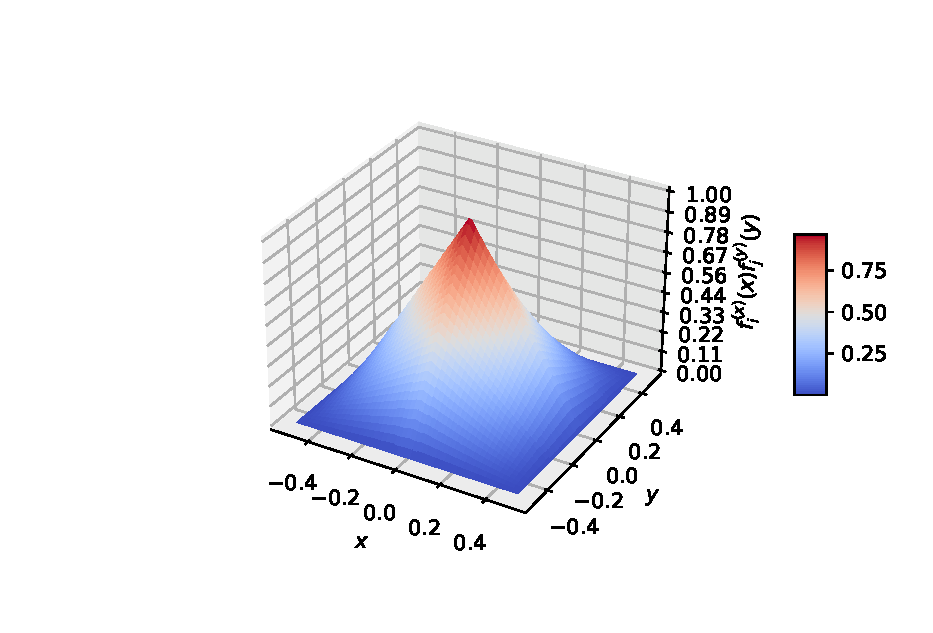
\includegraphics[width=0.8\textwidth]{./figuras/bilinearshape}
				\caption{Bilinear shape function on a rectangular grid.}
				\label{fig:3:bilinearshape}
			\end{figure}
		
			%Esta função pode representar melhor heterogeneidades nos espalhadores assim como o campo elétrico. No entanto, diferentemente da discretização por pulso,mais elementos contribuirão para o valor da função em um determinado ponto. Isso pode tornar o custo operacional da cálculo da integral \eqref{eq:3:discretization:11} mais caro, ao posso que pode melhorar a precisão da integração.
			This function can better represent heterogeneities in the scatterers as well as the electric field. However, unlike pulse discretization, more elements will contribute to the value of the function at a given point. This can make the computational cost of calculating the integral \eqref{eq:3:discretization:11} more expensive while improving integration accuracy.
			
			%Alternativamente às funções de tentativa definidas em apenas partes do domínio, existem os Métodos Espectrais no qual as funções de base são definidas em todo o domínio. A eficiência desse tipo de metodologia depende de uma escolha cuidadosa das funções, i.e., elas precisam ser uma boa representação das funções desconhecidas. IPor causa disso, esse tipo de estratégia para a discretização da função contraste pode não ser uma boa escolha. No entanto, isto pode ser compatível com a representação do campo elétrico principalmente porque, em problemas analíticos que envolvem apenas um espalhador, a solução é escrita em termos de exponenciais complexas ou funções de Bessel. Por exemplo, as funções $g^{(x)}_p(x)$ e $g^{(y)}_q(y)$ poderiam ser escolhidas de tal forma que:
			Alternatively to the trial functions defined in only pieces of the domain, the Spectral Methods define them everywhere in the domain. The efficiency of this sort of methodology depends on a careful choice of the functions, i.e., they need to be a good representation of the unknown functions. For this reason, applying such a strategy to contrast function discretization may not be a good choice, especially in the case of traditional geometries. However, this may be compatible with the representation of the electric field essentially because, in analytical problems that involve only a single scatterer, the solution is written in terms of complex exponentials or Bessel's functions. For example, the functions $g^{(x)}_p(x)$ and $g^{(y)}_q(y)$ could be chosen in such a way so that:
			\begin{align}
				g^{(x)}_p(x)g^{(y)}_q(x) = H^{(2)}_0(k_b\sqrt{(x_p-x)^2+(y_q-y)^2}) \label{eq:3:discretization:collocation:21} 
			\end{align}

			%Este exemplo de escolha remete à Colocação de Norma Mínima. Nesta abordagem, em um problema inverso linear cujo o operador $\mathcal{K} : X\rightarrow C[a,b]$ é linear, limitado e injetivo de um espaço de Hillbert $X$ em um espaço $C[a,b]$ de funções contínuas em $[a,b]$; então a função de tentativa pode ser definida como aquela cuja norma $L^2(a,b)$ é mínima. Esta solução, no caso de uma equação integral como em \eqref{eq:app:functional:4}, é o kernel $k_i(s) = k(t_i,s)$ o qual pertence a $L^2(a,b)$ \citep{kirsch2011introduction}.
			This choice example refers to the Minimum Norm Collocation. Theoretically, supposing a linear inverse problem whose operator $\mathcal{K} : X\rightarrow C[a,b]$ is linear, bounded, and injective of a space of Hillbert $X$ in a space $C[a,b]$ of continuous functions in $[a,b]$; then the trial function can be defined as the one whose norm $L^2(a,b)$ is minimum. This solution, in the case of an integral equation as in \eqref{eq:app:functional:4}, is the kernel $k_i(s) = k(t_i,s)$, which belongs to $L^2(a,b)$ \citep{kirsch2011introduction}.
			
			%De qualquer maneira, uma atenção especial sobre possíveis singularidades precisa ser tomada. Por causa disso, a descrição analítica e implementação desse tipo de método podem ser mais complexas.
			Nevertheless, exceptional attention to possible singularities needs to be taken. For this reason, the analytical description and implementation of this kind of method might be more complex.
		
		\subsection{The Galerkin Method}\label{chap:methods:discretization:galerkin}
			
			%Uma outra possilidade é escolher a função peso da mesma família das funções de tentativa, i.e.:
			Another possibility is to choose the weight function from the same family as the trial ones, i.e.:
			\begin{equation}
				w_k(x) = f_i(x) \label{eq:3:discretization:galerkin:0}
			\end{equation}
		
			%Esta estratégia é conhecida na literatura como Método do Galerkin ou Bubnov-Galerkin. Para problemas modelados a partir de equações diferenciais, a escolha dessas funções precisa atender os seguintes critérios \citep{fletcher1984computational}:
			This strategy is known in the literature as the Galerkin or Bubnov-Galerkin Method. For problems modeled from differential equations, the choice of these functions need to meet the following criteria \citep{fletcher1984computational}:
			\begin{enumerate}
				\item The weight and trial functions are chosen from the same family;
				\item Weight and trial functions must be linearly independent;
				\item The weight and trial functions must be the first N members of a dense set of functions;
				\item The weight and trial functions must satisfy the essential homogeneous boundary conditions exactly.
			\end{enumerate}
			%Enquanto a primeira condição define o método, a segunda diz respeito à relação entre equações linearmente independentes e variáveis desconhecidas. As duas últimas estão relacionadas com a eficiência do método.
			While the first condition defines the method, the second concerns the relationship between linearly independent equations and unknown variables. % The last two are related to the efficiency of the method.
		
			%No entanto, é necessário observar que, em EISP, os domínios das funções de peso e tentativa são diferentes, i.e., os argumentos das funções em \eqref{eq:3:discretization:galerkin:0} são diferentes. Além disso, é necessário integrar $E_{z_s}$ em todo o domínio $D$ \eqref{eq:3:discretization:9}. Este é um requisito que pode inviabilizar a aplicação prática do método visto que geralmente o campo espalhado só é conhecido em um conjunto finito de pontos. Uma alternativa para este problema é usar um método de interpolação. No entanto, esta estratégia pode induzir o método de inversão a soluções distantes da verdadeira.
			However, it is necessary to note that, in EISP, the domains of the weight and trial functions are different, i.e., their arguments in \eqref{eq:3:discretization:galerkin:0} are unrelated. In addition, it is necessary to integrate $E_{z_s}$ across the $D$ domain \eqref{eq:3:discretization:9}. This requirement can make the practical application of the method unfeasible since the scattered field is known only at a finite set of points. An alternative for this problem is to use an interpolation method. However, this strategy can induce the inversion to solutions far from the real one.
			
			%Por fim, podemos mencionar alguns dos poucos trabalhos na literatura que proporam metodologias baseadas nesse tipo de discretização. Ao invés de discretizarem a equação integral, \cite{zakaria2010finite} se basearam na equação da onda \eqref{eq:2:waveequations:final}. A equação diferencial foi escrita em termos do campo espalhado e da fonte de corrente. Além disto, foi imposta a condição de contorno de radiação de Sommerfield, modelada a partir de condições de absorção de segunda ordem. A partir disso, os autores utilizaram uma discretização por elementos triangulares não-uniformes e desenvolveram uma metodologia baseada na Inversão de Fonte de Contraste (a qual será explicada mais à frente no texto). Alternativamente, \cite{brown2019hybridizable} proporam uma abordagem híbrida e discontínua do Método do Galerkin para resolver o problema direto dentro do escopo da Inversão de Fonte de Contraste, a qual necessita de um número menor de graus de liberdade.
			Finally, we can mention some of the few papers in the literature that used methodologies based on this type of discretization. Rather than discretizing the integral equation, \cite{zakaria2010finite} applied it to the wave equation \eqref{eq:2:waveequations:final}. The differential equation was written in terms of the scattered field and the source. In addition, the Sommerfield radiation boundary condition was imposed, modeled with second-order absorption conditions. The authors used a non-uniform triangular elements discretization and developed a methodology based on the Contrast Source Inversion (which will be explained later in the text). Alternatively, \cite{brown2019hybridizable} proposed a hybrid and discontinuous approach to the Galerkin Method to solve the problem within the scope of the Contrast Source Inversion, which requires fewer degrees of freedom.
		
		\subsection{Some Aspects on Discretization}\label{chap:methods:discretization:aspects}
		
			%Antes de concluir a seção, dois aspectos também merecem destaque na discussão sobre discretizatição. Primeiramente, é preciso destacar que metodologias de discretização também são estratégias de regularização tal qual definido na \Autoref{chap:problemstatement:inverse} \citep{kirsch2011introduction}. A discretização é um assunto dentro do escopo de operadores de projeção. Matematicamente, um operador de projeção é definido da seguinte forma:
			Before concluding the section, two aspects also deserve to be highlighted when discussing discretization. First, it is necessary to underline that discretization methodologies are also regularization strategies, as defined in Section \ref{chap:problemstatement:inverse} \citep{kirsch2011introduction}. Discretization is an issue within the scope of projection. Mathematically, a projection operator is defined as follows:
			\vspace{1.5ex}
			\begin{definition}\label{def:3:projection}
				Projection Operator\\
				Let $X$ be a normed space over the field $\mathbb{K}=\mathbb{R}$ or $\mathbb{K}=\mathbb{C}$. Let $U\subset X$ be a closed subspace. A linear bounded operator $\mathcal{P} : X\rightarrow X$ is called a projection operator on $U$ if
				\begin{itemize}
					\item $\mathcal{P}\{x\} \in U, ~\forall x\in X$ and
					\item $\mathcal{P}\{x\} = x,~ \forall x\in U$.
				\end{itemize}
			\end{definition}
			\vspace{1.5ex}
			%Dentro deste contexto, ass funções de peso e tentativa são membras de subespaços de dimensão finita $X_n\subset X$ e $Y_n\subset Y$, respectivamente. Então, para um dado $y\in Y$ no qual $\mathcal{K}\{x\} = y$ é linear e um-pra-um, a discretização é operador de projeção $\mathcal{Q}_n : Y\rightarrow Y_n$ que resolve a equação:
			Within this context, the weight and trial functions are members of finite-dimension subspaces $X_n\subset X$ and $Y_n\subset Y$, respectively. Then, for a given $y\in Y$ in which $\mathcal{K}\{x\} = y$ is linear and one-to-one, discretization is a projection operator $\mathcal{Q}_n : Y\rightarrow Y_n$ that solves the equation:
			\begin{equation}
				\mathcal{Q}_n\left\{ K\{x_n\} \right\} = \mathcal{Q}_n\{y\} \label{eq:3:discretization:projection:0}
			\end{equation}
			
			%\noindent para $x_n\in X_n$. Então, seja $\{\hat{x}_1,\cdots,\hat{x}_n\}$ e $\{\hat{y}_1,\cdots,\hat{y}_n\}$ bases de $X_n$ e $Y_n$, respectivamente. Os termos $\mathcal{Q}_n\{y\}$ e $\mathcal{Q}_n\left\{ K\{x_n\}\right\}$ pode ser representados na seguinte forma:
			\noindent for $x_n\in X_n$. So, let $\{\hat{x}_1,\cdots,\hat{x}_n\}$ and $\{\hat{y}_1,\cdots,\hat{y}_n\}$ be bases of $X_n$ and $Y_n$, respectively. The terms $\mathcal{Q}_n\{y\}$ and  $\mathcal{Q}_n\left\{ K\{x_n\}\right\}$ can be represented as follows:
			\begin{align}
				\mathcal{Q}_n\{y\} &= \sum\limits_{i=1}^n b_i\hat{y}_i, ~~~~j=1,\cdots,n \label{eq:3:discretization:projection:1} \\
				\mathcal{Q}_n\left\{ K\{x_n\}\right\} &= \sum\limits_{i=1}^n A_{ij}\hat{y}_i, ~~j=1,\cdots,n \label{eq:3:discretization:projection:2}
			\end{align}
		
			%\noindent no qual $b_{i}$, $A_{ij}\in\mathbb{K}$. A combinação linear $x_n = \sum_{j=1}^n a_j\hat{x}_j$ é solução de \eqref{eq:3:discretization:projection:0} se e somente se $\{a_1,\cdots,a_n\} \in \mathbb{K}^n$ é solução do sistema finito de equações lineares:
			\noindent in which $b_{i}$, $A_{ij}\in\mathbb{K}$. The linear combination $x_n = \sum_{j=1}^n a_j\hat{x}_j$ is a solution of \eqref{eq:3:discretization:projection:0} if and only if $\{a_1,\cdots,a_n\} \in \mathbb{K}^n$ is a solution of the finite system of linear equations:
			\begin{equation}
				\sum\limits_{i=1}^n A_{ij} a_j = b_i, ~~ i=1,\cdots,n \label{eq:3:discretization:projection:3}
			\end{equation}
			
			%Neste contexto, o Método da Colocação é um exemplo de método de projeção cujo operador é denominado operador de interpolação. Já o Método do Galerkin é conhecido como um operador de projeção ortogonal.
			In this context, the Collocation Method is an example of a projection method whose operator is called an interpolation one. The Galerkin Method is known as an orthogonal projection operator. This implies that the error is orthogonal to the approximation space and the solution is the best one (minimum error) in that approximation space.
			
			%Em segundo lugar, a escolha do tamanho do conjunto de funções de peso e de tentativa ($N_U$, $N_V$, $N_I$, $N_J$, $N_P$, $N_Q$ e $N_S$) precisam levar em conta não só os aspectos discutidos sobre graus de liberdade na \Autoref{chap:problemstatement:eisp:5} mas também um conceito conhecido na literatura como Crime Inverso. Como destacou \cite{colton2019inverse}, é necessário que, quando a experimentação de métodos para EISP envolver dados sintéticos gerados por resolvedores diretos, este último não deve ter conexões com o resolvedor inverso. Em outras palavras, em um problema inverso de dimensão finita, é necessário evitar soluções triviais.
			Second, the choice of trial functions, i.e., its shape and size, needs to consider not only the aspects discussed about degrees of freedom in Subsection \ref{chap:problemstatement:eisp:5} but also a concept in the literature known as Inverse Crime. As highlighted by \cite{colton2019inverse}, it is necessary that, when the experimentation involves synthetic data generated by direct solvers, the latter must not have connections with the inverse solver. In other words, in an inverse problem of finite dimension, trivial solutions should be avoided.
			
			%O conceito pode ser exemplificado através de um problema genérico onde é o objetivo é recuperar uma família $G_m$ de superfícies de contorno com $m$ parâmetros. Se, para este problema, utilizarmos dados sintetizados por um resolvedor direto \textbf{M} para obter $n$ dados de entrada, como por exemplo, amostras de campo distante. Isto equivale a uma função $g : \mathbb{R}^m \rightarrow \mathbb{C}^n$. Portanto, se uma determinada superfície $\partial D\in G_m$ é gerada a partir do conjunto de parâmetros $a_0$, um método de inversão que incorpora o mesmo resolvedor direto \textbf{M} não está fazendo nada mais do que resolver o problema de dimensão finita $g(a) = g(a_0)$. Por isso, a superfície $\partial D$ será inevitavelmente bem reconstruída, pressupondo que $m$ e $n$ não são grandes demais.
			The concept can be illustrated through a generic problem where its objective is to recover a family $G_m$ of contour surfaces with $m$ parameters. For this problem, if we use data synthesized by a direct resolver \textbf{M} to obtain $n$ input data, such as distant field samples, this is equivalent to a function $g : \mathbb{R}^m \rightarrow \mathbb{C}^n$. Therefore, if a given surface $\partial D\in G_m$ is generated from the set of parameters $p_0$, an inversion method that incorporates the same direct solver \textbf{M} is doing nothing more than solving the finite dimension problem $g(p) = g(p_0)$. Therefore, the $\partial D$ surface will inevitably be well reconstructed, assuming that $m$ and $n$ are not too big.
			
			%\cite{wirgin2004inverse} trouxe mais contribuições para o assunto através da análise de três exemplos os quais, mesmo não sendo universais, aprofundaram o entendimento sobre o conceito introduzido por \cite{colton2019inverse}. As conclusões feitas por Wirgin podem ser resumidas em:
			\cite{wirgin2004inverse} brought more contributions to the subject by analyzing three examples that, although not universal, deepened the understanding of the concept introduced by \cite{colton2019inverse}. The conclusions made by Wirgin can be summarized in:
			\begin{itemize}
				\item Regarding the meaning of the lack of connection between a direct solver and an inverse one, he proposed that its practical meaning is the difference in the number of terms of the power series representing the forward and inverse solver. That is, if that number of terms are different, then there would be no connection.
				%\item Wirgin concluiu que quanto maior a diferença entre ambas as partes em termos de seus funcionais, maior o erro relativo da inversão. Isso significa que reconstruir os parâmetros com muita precisão são é possível quando os dois resolvedores têm conexão.
				\item Wirgin concluded that the more significant difference between both solvers in terms of their functionals, the larger relative inversion error. That means recovering the parameters very accurately is possible when the two resolvers are connected.
				%\item Cometer o crime inverso também tem o sentido prático de pelo menos revelar se o problema inverso tem ou não solução única.
				\item Committing the inverse crime also has the practical sense of at least revealing whether the inverse problem has a unique solution or not.
				%\item Quando o crime inverso é cometido, a solução pode não ser somente a ``solução trivial'', mas também podem ser observadas outras por meio de um método numérico robusto, as quais não necessariamente seriam observadas numa situação onde o crime não é cometido. 
				\item When the inverse crime is committed, the solution may not only be the ``trivial'' one, but others can also be observed through a robust numerical method system, which would not necessarily be observed in a situation where the crime is not committed.
			\end{itemize}
		
			%Wirgin também critica o uso do termo ``solução trivial'' para o assunto uma vez que o objetivo é de fato reconstruir os parâmetros com maior precisão possível. Além disso, mesmo que sua análise matemática se baseie na reconstrução de um único parâmetro por um único dado, a análise matemática para problema maiores, inclusive dois parâmetros e dois dados, se torna muito mais complicada. No entanto, ele afirma que seria difícil de esperar contradições entre suas conclusões para um caso mais simples e as que porventura poderiam ser obtidas para casos mais complexos. Por fim, em experimentos com dados reais não faz sentido a preocupação com o crime inverso uma vez que, na verdade, o ``resolvedor direto'' é desconhecido. Mesmo que um resolvedor direto represente mimetize bem o fenômeno físico, isso não impede que se observe perturbações na solução que representem algo falso.
			Wirgin also criticizes the use of the term ``trivial solution'' since the objective is, in fact, to recover the parameters as accurately as possible. In addition, even if his mathematical analysis is based on the reconstruction of a single parameter for a single data, mathematical analysis for larger problems, including two parameters and two data, becomes much more complicated. However, he claims that it would be difficult to expect contradictions between their conclusions for a simple case and those that might be obtained for more complex ones. Finally, in experiments with real data, it does not make sense to worry about inverse crime since, in fact, the ``direct resolver'' is unknown. Even that a direct solver represents the physical phenomenon well, this does not prevent the observation of disturbances in the solution, representing something false.
		
	\section{The Linear Case}\label{chap:methods:linear}
			
		%Embora EISP seja não-linear, o estudo do caso linear é muito importante pelo motivo que muitos métodos utilizam estratégias de linearização do problema. Estas estratégias podem ser importantes tanto para definir direções de busca como para definir soluções iniciais. Além disso, é possível utilizar aproximações para o campo total para problemas que pressupõem espalhadores fracos. Neste caso, o problema se torna linear. Isto possibilita a utilização das metodologias clássicas de regularização de operadores lineares compactos e limitados. A discretização de \eqref{eq:3:discretization:collocation:3} e \eqref{eq:3:discretization:10} serão utilizadas para discutir as metodologias traditionais. No entanto, todas essas metodologias podem ser facilmente adaptadas para as outras equações e discretizações.
		%Although EISP is non-linear, the study of the linear case is significant because many methods use strategies based on problem linearization. These strategies can be essential when defining search directions and initial solutions. In addition, it is possible to use approximations for the total field in problems where we assume weak scatterers. In this case, the problem may be approximated to a linear one. This approximation enables the use of traditional regularization methodologies for compact and bounded linear operators. The discretization of \eqref{eq:3:discretization:collocation:3} and \eqref{eq:3:discretization:10} will be used to discuss them. However, all of these methodologies can be easily adapted to other equations and discretizations.
		Although EISP is non-linear, the study of the linear case is significant because many methods use strategies based on problem linearization. These strategies can be essential when defining search directions and initial solutions. In addition, it is possible to use approximations for the total field in problems where we assume weak scatterers. In this case, the problem may be approximated to a linear one. The discretization of \eqref{eq:3:discretization:collocation:3} and \eqref{eq:3:discretization:10} will be used to discuss them. However, all of these methodologies can be easily adapted to other equations and discretizations.
			
		\subsection{Approximated Solutions for Weak Scatterers}\label{chap:methods:linear:weak}
				
			%Quando as propriedades dielétricas de um espalhador diferem muito pouco do meio de fundo, ele é considerado um espalhador fraco. Nestas condições, é possível fazer aproximações em relação ao campo elétrico e tornar o problema linear. Existem duas técnicas clássicas que abordam esta situação: a Aproximação de Born (BA) e a Aproximação de Rytov (RA). A primeira é mais adequada para baixas frequências enquanto que a segunda é mais adequada para altas.
			When the dielectric properties of a scatterer differ very little from the background, and its size is not too large, it is considered a weak one (DNL $\ll1$). Under these conditions, it is possible to approximate the electric field and turn the problem into a linear one. Two classic techniques address this situation: the Born Approximation (BA) and the Rytov Approximation (RA). The first is best suited for low frequencies, while the second is more suitable for high ones.
			
			%A série de Born é uma metodologia a qual escreve o campo elétrico como uma série em termos da função de Green, do contraste e do campo incidente. Se a norma $L^2(S)$ na qual $||\int_S d\mathbf{r^\prime} \mathbf{\bar{G}}(\mathbf{r},\mathbf{r^\prime})\chi(\mathbf{\mathbf{r^\prime}})||<1$, então:
			Born's series is a methodology that writes the electric field as a series in terms of Green's function, contrast, and incident field. Recapitulating the formulas from Subsection \ref{chap:problemstatement:eisp:4}, if the $L^2(S)$-norm $$\left\|\int_S d\mathbf{r^\prime} \mathbf{\bar{G}}(\mathbf{r},\mathbf{r^\prime})\chi(\mathbf{\mathbf{r^\prime}})\right\|<1,$$ then:
			\begin{equation}
				\mathbf{E}(\mathbf{r}) = \sum\limits_{n=0}^\infty \left(\int_Sd\mathbf{r^\prime} \mathbf{\bar{G}}(\mathbf{r},\mathbf{r^\prime})\chi(\mathbf{r^\prime})\right)^n\mathbf{E}_i(\mathbf{r}) \label{eq:3:linear:bornseries:analytic}
			\end{equation}
			
			%Seguindo a forma matricial \eqref{eq:3:discretization:collocation:11}, \eqref{eq:3:linear:bornseries:analytic} pode ser escrita de maneira discretizada como:
			Following the matrix form \eqref{eq:3:discretization:collocation:11}, \eqref{eq:3:linear:bornseries:analytic} can be written in a discretized fashion as:
			\begin{equation}
				\mathbf{\bar{E}} = \sum\limits_{n=0}^\infty (\mathbf{\bar{G}^S}\boldsymbol{\bar{\chi}})^n\mathbf{\bar{E}^i} \label{eq:3:linear:bornseries:discrete}
			\end{equation}
			
			%A Aproximação de Born de Primeira-Ordem é uma single-scattering approximation obtida a partir da truncamento da série de Born \eqref{eq:3:linear:bornseries:analytic} em seu primeiro termo $n=0$, i.e.:
			The First-Order Born Approximation is a single-scattering approximation obtained from the truncation of the Born series \eqref{eq:3:linear:bornseries:analytic} in its first term $n = 0$, i.e.:
			\begin{equation}
				\mathbf{E}(\mathbf{r}) \approx \mathbf{E}_i(\mathbf{r}) \label{eq:3:linear:bornapproximation}
			\end{equation}		
			
			%Convém destacar que \eqref{eq:3:linear:bornapproximation} é também equivalente a uma aproximação de primeira-ordem da expansão em séries de Neumman da equação integral \eqref{eq:2:eisp:2} e a uma aproximação por séries de Taylor de $\mathbf{E}(\mathbf{r})$ \citep{chew1995}.
			
			%Embora ela até viole o princípio de conservação de energia, o teorema da reciprocidade é ainda válido por causa da simetria da função diádica de Green \citep{chew1995}. Além disso, se o tamanho do espalhador é da ordem $L$ no qual $k_bL \ll 1$, então a função diádica de Green \eqref{eq:app:green:17}, o contraste e a integral volumétrica podem ser aproximadas por \citep{chew1995}:
			Although it even violates the energy conservation principle, the reciprocity is still valid because of the symmetry of dyadic Green's function \citep{chew1995}. In addition, if the size of the scatterer is of the order $L$ in which $k_bL \ll 1$, then dyadic Green's function \eqref{eq:app:green:17}, contrast and volumetric integral can be approximated by \citep{chew1995}:
			\begin{align}
				\mathbf{\bar{G}}(\mathbf{r},\mathbf{r^\prime}) &\approx \left(1+\frac{1}{k_b^2L^2}\right)\frac{1}{L} \label{eq:3:linear:bornapproximation:1} \\
				k^2(\mathbf{r})-k_b^2 &\approx k_b^2\Delta\epsilon_r \label{eq:3:linear:bornapproximation:2} \\
				\int_D d\mathbf{r^\prime} &\approx L^3 \label{eq:3:linear:bornapproximation:3}
			\end{align}
			
			%\noindent onde $\Delta\epsilon_r = \epsilon_r/\epsilon_{rb} - 1$. Desta forma, \eqref{eq:2:eisp:2} é aproximada por:
			\noindent where $\Delta\epsilon_r = \epsilon_r/\epsilon_{rb} - 1$. Thus, \eqref{eq:2:eisp:2} is approximated by:
			\begin{equation}
				\mathbf{E}_s(\mathbf{r}) \approx \left[(k_bL)^2+1\right]\Delta\epsilon_r\mathbf{E}_i(\mathbf{r}) \label{eq:3:linear:bornapproximation:4}
			\end{equation}
		
			%No entanto, em situações onde a frequência é mais alta, a variação do campo dentro do objeto é preponderante. Nestes casos, o operador $\nabla\nabla$ é aproximado por $k_b^2$ e a fase do campo dentro do espalhador precisa ser levada em conta. Pressupondo que o campo dentro do espalhador é uma superposição de ondas planas, a aproximação de \eqref{eq:3:linear:bornapproximation} precisa ser corrigida para:
			However, in situations where the frequency is higher, the field variation inside the object is dominant. In these cases, the operator $\nabla\nabla$ is approximated by $k_b^2$ and the field phase within the scatterer needs to be taken into account. Assuming that the field inside the scatterer is a superposition of plane waves, the approximation in \eqref{eq:3:linear:bornapproximation} needs to be fixed to:
			\begin{equation}
				\mathbf{E}(\mathbf{r}) \approx \mathbf{E}_i(\mathbf{r})e^{j(\mathbf{k}-\mathbf{k_b})\cdot\mathbf{r}}  \label{eq:3:linear:bornapproximation:5}
			\end{equation}
		
			%Esta aproximação depende que $(k-k_b)L\ll1$, a qual é uma restrição mais forte que a anterior.
			This approximation depends on $(k-k_b)L\ll1$, which is a stronger constraint than the previous one.
			
			%A Aproximação de Primeira-Ordem de Rytov é baseada numa redução da equação vetorial por uma equação escalar. Esta redução consiste na substituição do campo total por uma exponencial complexa cuja fase é função, i.e.:
			Rytov's First-Order Approximation is based on a reduction in the vector equation by a scalar equation. This reduction consists of replacing the total field by a complex exponential whose phase is a function, i.e.:
			\begin{equation}
				E_z(\mathbf{r}) \approx E_{i_z}(\mathbf{r})^{\psi(\mathbf{r})} \label{eq:3:linear:rytov:0}
			\end{equation}
		
			%\noindent no qual a fase de primeira-ordem $\psi(\mathbf{r})$ é baseada no campo espalhado de \eqref{eq:2:eisp:2} calculado pela Aproximação de Born \eqref{eq:3:linear:bornapproximation}, i.e.:
			\noindent in which the first-order phase $\psi(\mathbf{r})$ is based on the scattered field of \eqref{eq:2:eisp:2} calculated by the Born Approximation \eqref{eq:3:linear:bornapproximation}, i.e.:
			\begin{equation}
				\psi(\mathbf{r}) = \frac{1}{E_i(\mathbf{r})} \int_S d\mathbf{r^\prime} g(\mathbf{r},\mathbf{r^\prime})E_{i_z}(\mathbf{r^\prime})\chi(\mathbf{r^\prime}) \label{eq:3:linear:rytov:1}
			\end{equation}
		
			%Aplicando uma análise semelhante a \eqref{eq:3:linear:bornapproximation:1}-\eqref{eq:3:linear:bornapproximation:3}, é possível demonstrar que $\psi(\mathbf{r}) \approx k_b^2L^2\Delta\epsilon_r$ quando $k_bL\rightarrow0$ \citep{chew1995}. Esta condição é equivalente a $(k_bL)^2\Delta\epsilon_r\ll1$. Por outro lado, se a frequência tende ao infinito, então $\psi(\mathbf{r}) \approx k_bL\Delta\epsilon_r$. A condição para esta aproximação é $\Delta\epsilon_r \ll 1$, a qual é muito mais fraca que a anterior. Por isso, esta aproximação é mais adequada para altas frequências.
			When we apply an analysis similar to \eqref{eq:3:linear:bornapproximation:1}-\eqref{eq:3:linear:bornapproximation:3}, it is possible to demonstrate that $\psi(\mathbf{r}) \approx k_b^2L^2\Delta\epsilon_r$ when $k_bL\rightarrow0$ \citep{chew1995}. This condition is equivalent to $(k_bL)^2\Delta\epsilon_r\ll1$. On the other hand, if the frequency tends to infinity, then $\psi(\mathbf{r}) \approx k_bL\Delta\epsilon_r$. The condition for this approximation is $\Delta\epsilon_r \ll 1$, which is much weaker than the previous one. Therefore, this approach is more suitable for high frequencies.
		
		\subsection{The Back-Propagation Method}\label{chap:methods:linear:backpropagation}
		
			The Back-Propagation (BP) Method is noniterative algorithm which is able to provide a solution for the contrast image. Such solution is often used as initial guess in many methods. The method is suitable for arbitrary incident fields, near and far fields measurements. BP is based on three steps: (i) estimate the induced current; (ii) compute total field in $S$ through the state equation; and (iii) determine the contrast image by relation between total field and induced current. If the induced current is assumed to be proportional to the back-propagation field, then the induced current is evaluated according to:
			\begin{equation}
				\mathbf{\bar{J}^{eq}} = \gamma \mathbf{\bar{G}^{D*}} \mathbf{\bar{E}^s} \label{eq:3:linear:bp:J}
			\end{equation}
		
			\noindent where the superscript $\mathbf{^*}$ is the operator's adjoint and numerically given by the conjugated-transposed. The parameter $\gamma$ is a complex value that is chosen to minimize the cost function defined as the quadratic error in the scattered field:
			\begin{equation}
				F(\gamma) = ||\mathbf{\bar{E}^s} - \mathbf{\bar{G}^D}(\gamma\mathbf{\bar{G}^{D*}}\mathbf{\bar{E}^s})||^2 \label{eq:3:linear:bp:F}
			\end{equation}
		
			The minimum of \eqref{eq:3:linear:bp:F} might be obtained analytically and is given as follows:
			\begin{equation}
				\gamma = \frac{\langle \mathbf{\bar{E}^s}, \mathbf{\bar{G}^D}\mathbf{\bar{G}^{D*}}\mathbf{\bar{E}^s}\rangle}{||\mathbf{\bar{G}^D}\mathbf{\bar{G}^{D*}}\mathbf{\bar{E}^s}||}
			\end{equation}

			\noindent where $\langle\cdot,\cdot\rangle$ is the inner product, which is numerically computed as the product between the transpose of the first argument and the complex conjugate of the second one.
			
			Once the induced current is obtained, then the total electric field might be evaluated according to \eqref{eq:3:discretization:collocation:11} replacing $\boldsymbol{\bar{\chi}}\mathbf{\bar{E}}$ by $\mathbf{\bar{J}^{eq}}$. Finally, the contrast might be evaluated according to:
			\begin{equation}
				\chi_{ij} = \frac{\sum\limits_{s=1}^{N_S}J^{eq}_{ijs}E^*_{ijs}}{\sum\limits_{s=1}^{N_S}|E^*_{ijs}|^2} \label{eq:3:linear:bp:x}
			\end{equation}
		
			If it is known that only lossless scatterers are present, then the imaginary part of $\boldsymbol{\bar{\chi}}$ can be neglected.
			
		\subsection{Dominant Current Scheme}\label{chap:methods:linear:dominantcurrent}
			
			In nonlinear problems with large number of variables, there may be some unknowns which are more relevant. Since recovering the induced current might be a hard task when a limited number of measurements are available, the dominant part of the induced current might be prioritized. Such strategy is based on the fact that the dominant current contains the most important features of the unknown scatterers and it is more robust against noise. This is the core idea behind the Dominant Current Scheme (DCS) \citep{wei2019deep}.
			
			When the Singular Value Decomposition is applied to $\mathbf{\bar{G}^D}$, the dominant current might be evaluated according to:
			\begin{equation}
				\mathbf{\bar{J}^{eq}}_+ = \sum\limits_{n=1}^L \frac{\bar{u}^*_n\cdot \mathbf{\bar{E}}^s}{\xi_n}\bar{v}_j \label{eq:3:linear:dcs:j+}
			\end{equation}
		
			\noindent where $\bar{u}$, $\bar{v}$, and $\xi$ are the left, right, and singular value vectors from the decomposition; and $L$ is an index that limits the singular values in descending order, i.e., the dominant current is computed taking into account the first $L$ largest singular values. Therefore, the $N_IN_J - L$ smallest singular values are neglected and unstable components corrupted by noise are avoided. However, a compensation for the missing information is also provided, i.e.:
			\begin{equation}
				\mathbf{\bar{J}^{eq}}_- = \mathbf{\bar{F}}\cdot\boldsymbol{\alpha} \label{eq:3:linear:dcs:j-}
			\end{equation}
		
			\noindent where $\mathbf{\bar{F}}$ and $\boldsymbol{\alpha}$ are the low-frequency matrices composed by the first $m$ low-frequency  Fourier bases and their corresponding coefficients, respectively. Since $\boldsymbol{\alpha}$ is an unknown, some approximation has to be made to complete the scheme. \cite{wei2019deep} proposed the following objective-function:
			\begin{equation}
				F(\boldsymbol{\alpha}) = \left[ \frac{||\mathbf{\bar{G}^F}\cdot\boldsymbol{\alpha}+\mathbf{\bar{G}^E}||^2}{||\mathbf{\bar{E}^s}||^2}+\frac{||\mathbf{\bar{A}}\cdot\boldsymbol{\alpha}+\mathbf{\bar{B}}||^2    }{||\mathbf{\bar{J}^{eq}_+}||^2}\right] \label{eq:3:linear:dcs:f}
			\end{equation}
		
			\noindent where $\mathbf{\bar{G}^F} = \mathbf{\bar{G}^D}\cdot\mathbf{\bar{F}}$, $\mathbf{\bar{G}^E} = \mathbf{\bar{G}^D}\cdot\mathbf{\bar{J}^{eq}}_+ - \mathbf{\bar{E}^s}$, $\mathbf{\bar{A}} = \mathbf{\bar{F}} -\boldsymbol{\bar{\chi}}\cdot\mathbf{\bar{G}^s}\cdot\mathbf{\bar{F}}$, and $\mathbf{\bar{B}} = \boldsymbol{\bar{\chi}}(\mathbf{\bar{E}^i}+\mathbf{\bar{G}^S}\mathbf{J^{eq}}_+)-\mathbf{J^{eq}_-}$.
			
			Based on \eqref{eq:3:linear:dcs:f}, the authors proposed an iterative process to update $\boldsymbol{\bar{\chi}}$ and $\boldsymbol{\alpha}$, starting by $\boldsymbol{\bar{\chi}}=\mathbf{0}$. The variable $\boldsymbol{\alpha}$ is approximated according to $\boldsymbol{\alpha} = \beta\boldsymbol{\gamma}$ where:
			\begin{eqnarray}
				\boldsymbol{\gamma} &=& \left( \frac{\mathbf{\bar{G}^{F*}}\cdot\mathbf{\bar{G}^E}}{||\mathbf{\bar{E}^s}||^2}-\frac{\mathbf{\bar{A}^{*}}\cdot\mathbf{\bar{B}}}{||\mathbf{\bar{J}^{eq}}||^2}\right) \label{eq:3:linear:dcs:rho} \\
				\beta &=& \frac{Num}{Den} \\
				Num &=& -\frac{\mathbf{\bar{G}^{F*}}\cdot\boldsymbol{\gamma}\cdot\mathbf{\bar{G}^E}}{||\mathbf{\bar{E}^s}||^2} + \frac{(\mathbf{\bar{A}}\cdot\boldsymbol{\gamma})^{*}\cdot\mathbf{\bar{B}}}{||\mathbf{\bar{J}^{eq}_+}||^2} \\
				Den &=& \frac{||\mathbf{\bar{G}^{F}}\cdot\boldsymbol{\gamma}||^2}{||\mathbf{\bar{E}^s}||^2} + \frac{||\mathbf{\bar{A}}\cdot\boldsymbol{\gamma}||^2}{||\mathbf{\bar{J}^{eq}_+}||^2}
			\end{eqnarray}
		
			Then, after using $\boldsymbol{\alpha}$ to compute the low-frequency compensation through \eqref{eq:3:linear:dcs:j-}, the following steps are required:
			\begin{eqnarray}
				\mathbf{\bar{J}^{eq}} &=& \mathbf{\bar{J}^{eq}_+} + \mathbf{\bar{J}^{eq}_-} \\
				\mathbf{\bar{E}} &=& \mathbf{\bar{E}^i} + \mathbf{\bar{G}^S}\mathbf{\bar{J}^{eq}} \\
				\chi_{ijs} &=& \frac{J^{eq}_{ijs}E_{ijs}^*}{||E_{ijs}||^2} \label{eq:3:linear:dcs:x}
			\end{eqnarray}
		
			In \eqref{eq:3:linear:dcs:x}, it is computed one contrast image for each incidence. The authors had decided for this based in its application to Convolution Neural Networks. However, a computation similar to \eqref{eq:3:linear:bp:x} might also be used.

	\section{Regularization Methods}\label{chap:methods:regularization}
	
		Whenever the total electric field in the state space is known, the inverse problem turns into a linear one. This may happen when approximating the total field by the incident one (subsection \ref{chap:methods:linear:weak}) or when a forward solver is employed to determine it for a given outdated contrast image. For a linear problem, regularization methods might be applied to solve an inverse problem which usually has more unknowns than equations. In the next subsections, traditional regularization methods will be covered.

		\subsection{The Tikhonov Regularization}\label{chap:methods:linear:tikhonov}
			
			%Talvez a mais conhecida técnica de regularização de problemas inversos com operadores lineares e limitado é a Regularização de Tikhonov \citep{tikhonov1963regularization,kirsch2011introduction}. Não somente nesse caso como também em sistemas de equações lineares superdeterminados, i.e., onde o número de equações é menor que o de variáveis. De um modo geral, o princípio deste método é determinar a solução $x\in X$ que minimiza $||\mathcal{K}\{x\} = y||$ para alguma norma em $Y$. Se $X$ tem dimensão finita e $\mathcal{K}$ é compacto, o problema de minimização também é mal-posto.
			Perhaps the most traditional technique for regularizing inverse problems with linear and limited operators is the Tikhonov Regularization \citep{tikhonov1963regularization,kirsch2011introduction}. Not only in this case but also in underdetermined systems of equations, i.e., where the number of equations is less than that of variables. In general, the principle of this method is to determine the solution $x\in X$ that minimizes $||\mathcal{K}\{x\} = y||$ for some norm in $Y$. If $X$ has a finite dimension and $\mathcal{K}$ is compact, then the minimization problem is also ill-posed.
			
			%A Regularização de Tikhonov propõe determinar uma solução $x^\alpha\in X$ a qual minimiza o funcional de Tikhonov $J_\alpha$:
			The Tikhonov Regularization proposes to determine a solution $x^{\alpha_T}\in X$ which minimizes the Tikhonov's functional $J_{\alpha_T}$\footnote{Another possible interpretation for the Tikhonov Regularization was recently proposed by \cite{gerth2021new}. The author has observed that the exact solution is estimated from the range of the adjoint operator and the properties are derived through the concept of approximate source conditions.}:
			\begin{equation}
				J_{\alpha_T}(x) \coloneqq ||\mathcal{K}\{x\}-y||^2 + \alpha_{T}||x||^2 \label{eq:3:linear:tikhonov:functional}
			\end{equation}

			%\noindent no $\alpha_{T} > 0$ é uma constante e $X$ e $Y$ são espaços de Hilbert. Nesse caso, $x^\alpha$ é solução de:
			\noindent in which $\alpha_{T} > 0$ is a constant and $X$ and $Y$ are Hilbert spaces. In this case, $x^{\alpha_T}$ is the solution of:
			\begin{equation}
				\alpha_Tx^{\alpha_T} + \mathcal{K}^*\{\mathcal{K}\{x^\alpha\}\} = \mathcal{K}^*\{y\} \label{eq:3:linear:tikhonov:equation}
			\end{equation}
		
			%\noindent onde $\mathcal{K}^*$ é o operador adjunto de $\mathcal{K}$. Portanto, a solução $x^\alpha$ pode ser escrita na forma de \eqref{eq:2:inverse:2} através:
			\noindent where $\mathcal{K}^*$ is the adjoint operator of $\mathcal{K}$. Therefore, the solution $x^{\alpha_T}$ can be written in the form in \eqref{eq:2:inverse:2} through
			\begin{equation}
				\mathcal{R}_{\alpha_T} \coloneqq \left(\alpha_T\mathcal{I} + \mathcal{K}^*\mathcal{K}\right)^{-1}\mathcal{K}^* : Y \rightarrow X \label{eq:3:linear:tikhonov:operator}
			\end{equation}
			
			%\noindent onde $\mathcal{I}$ é o operador identidade. O sistema linear \eqref{eq:3:linear:tikhonov:equation} também pode ser escrito como:
			\noindent where $\mathcal{I}$ is the identity operator. The linear system \eqref{eq:3:linear:tikhonov:equation} can also be written as:
			\begin{equation}
				\left(\alpha_T\mathcal{I} + \mathcal{K}^*\mathcal{K}\right)x^{\alpha_T} = \mathcal{K}^*\{y\} \label{eq:3:linear:tikhonov:linearsystem}
			\end{equation}
		
			%O limite superior do erro para essa aproximação é conhecido e expresso em termos da norma do erro em $y$, i.e., $||y-y^\delta||\le\delta$; e em termos de uma constante $E$ tal que $||z||\le E$ e $x=\mathcal{K}^*\{z\}\in\mathcal{K}^*\{Y\}$. Neste caso, se $\alpha_T(\delta) = c\delta/E$ para um $c>0$, então \citep{kirsch2011introduction}:
			The upper limit of the error for this approximation is known and expressed in terms of the norm of error in $y$, i.e., $||y-y^\delta||\le\delta$; and in terms of a constant $\Delta$ such that $||z||\le\Delta$, $x=\mathcal{K}^*\{z\}\in\mathcal{K}^*\{Y\}$, and $z\in Y$. In this case, if $\alpha_T(\delta) = c\delta/\Delta$ for a $c>0$, then the error of the solution $x^{\alpha_T(\delta),\delta}$, which is based on these assumptions, follows below \citep{kirsch2011introduction}:
			\begin{equation}
				||x^{\alpha_T(\delta),\delta}-x|| \le \frac{1}{2}\left(1/\sqrt{c}+\sqrt{c}\right)\sqrt{\delta E} \label{eq:3:linear:tikhonov:error:1}
			\end{equation}
		
			%Por um outro lado, se a função auxiliar $z$ é definida como $x=\mathcal{K}\{\mathcal{K}^*\{z\}\}\in\mathcal{K}\{\mathcal{K}^*\{X\}\}$ e a escolha $\alpha_{T}(\delta) = c(\delta/E)^{2/3}$ para um $c>0$, então o limite superior do erro será \citep{kirsch2011introduction}:
			On the other hand, if the auxiliary function $z$ is defined as$x=\mathcal{K}\{\mathcal{K}^*\{z\}\}\in\mathcal{K}\{\mathcal{K}^*\{X\}\}$ and choosing $\alpha_{T}(\delta) = c(\delta/\Delta)^{2/3}$ for a $c>0$, then the upper limit of the error it will be \citep{kirsch2011introduction}:
			\begin{equation}
				||x^{\alpha_T(\delta),\delta}-x|| \le \left(\frac{1}{2\sqrt{c}}+c\right)\Delta^{1/3}\delta^{2/3} \label{eq:3:linear:tikhonov:error:2}
			\end{equation}
		
			%Em outras palavras, \eqref{eq:3:linear:tikhonov:error:1} e \eqref{eq:3:linear:tikhonov:error:2} estabelecem que a regularização de Tikhonov é ótima dada informação $||\left(\mathcal{K}^*\right)^{-1}\{x\}||\le E$ ou $||\left(\mathcal{K}^*\mathcal{K}\right)^{-1}\{x\}||\le E$, desde que $\mathcal{K}^*$ seja um-pra-um.
			In other words, \eqref{eq:3:linear:tikhonov:error:1} and \eqref{eq:3:linear:tikhonov:error:2} establish that Tikhonov regularization is optimum given information $||\left(\mathcal{K}^*\right)^{-1}\{x\}||\le \Delta$  or $||\left(\mathcal{K}^*\mathcal{K}\right)^{-1}\{x\}||\le \Delta$, provided that $\mathcal{K}^*$ is an one-to-one operator.
			
			%Vale à pena destacar que, de uma forma prática, o método de regularização corrige os autovalores do sistema. Em outras palavras, se os autovalores de $\mathcal{K}$ tendem a zero devido a sua má-posição, os de $\alpha_{T}\mathcal{I} + \mathcal{K}^*\mathcal{K}$ são estabelecidos acima de zero por $\alpha_T>0$. Destaca-se também a relação entre a escolha de $\alpha_T$ e $\delta$. Esta relação é tal que $\alpha_T$ tende a zero quando $\delta\rightarrow0$. No entanto a velocidade de convergência não chega a ser da ordem de $\delta^2$. Além disso, quanto mais suave $x$ é, mais devagar $\alpha_T$ tenderá a zero. Portanto, em situações onde já é conhecido que a suavidade é um aspeto predominante da solução $x$, o método de regularização de Tikhonov não é ótimo. Nestes casos, os métodos de Landweber e do Gradiente-Conjugado, os quais serão discutidos em breve, têm melhor desempenho.
			It is worth noting that the regularization method is also a correction to the eigenvalues of the system. In other words, if the eigenvalues of $\mathcal{K}$ tend to zero due to their ill-posedness, those of $\alpha_{T}\mathcal{I} + \mathcal{K}^*\mathcal{K}$ are established above zero by $\alpha_T>0$. Also highlighted is the relationship between the choice of $\alpha_T$ and $\delta$. This relationship is such that $\alpha_T$ tends to zero when $\delta\rightarrow0$. Also, the smoother $x$ is, the slower $\alpha_T$ will tend to zero. Therefore, in situations where it is already known that smoothness is a predominant aspect of solution $x$, the Tikhonov regularization method is not optimal. In these cases, the Landweber and Gradient-Conjugate methods, which will be discussed soon, perform better.
			
			%O método pode ser aplicado na equação matricial \eqref{eq:3:discretization:collocation:10}. Para isso, é necessário definir o vetor-coluna $\boldsymbol{\chi}$ o qual representa a diagonal principal de $\boldsymbol{\bar{\chi}}$ e o vetor-coluna $\mathbf{\bar{E}}^{\mathbf{s}F}$\footnote{No restante do texto, o operador ``$^F$'' sempre será utilizado com o significado de transformação de matriz em vetor-coluna. A ordem será padronizada em coluna primeiro e linha depois. A letra $F$ foi escolhida com objetivo de remeter à palavra \textit{flatten}.} o qual é o rearranjo da matriz $\mathbf{\bar{E}^s}$ na seguinte forma:
			The method can be applied to the matrix equation \eqref{eq:3:discretization:collocation:10}. This is achieved if we define the column vector $\boldsymbol{\chi}$, which represents the main diagonal of $\boldsymbol{\bar{\chi}}$ and the column vector $\mathbf{\bar{E}}^{\mathbf{s}F}$ which is the rearrangement of the matrix $\mathbf{\bar{E}^s}$ in the following form\footnote{The ``$^F$'' operator will always mean transforming a matrix into a column vector throughout this thesis. The order will be standardized in column first and row after. The letter F was chosen in order to refer to the word flatten.}:
			\begin{equation}
				\mathbf{\bar{E}}^{\mathbf{s}F} =     \begin{bmatrix}
																			E^s_{11} \\ E^s_{12} \\ \vdots \\ E^s_{N_MN_S}
																		\end{bmatrix} \label{eq:3:columnvector}
			\end{equation}
			
			%Além disso, definiremos a matriz $\mathbf{\bar{K}}$ como:
			In addition, we will define the $\mathbf{\bar{K}}$ matrix as:
			\begin{equation}
				\mathbf{\bar{K}} = \begin{bmatrix}
											 G^D_{111}E_{111} & G^D_{112}E_{121} & \cdots & G^D_{1ij}E_{ij1} & \cdots & G^D_{1N_IN_J}E_{N_IN_J1} \\
											 G^D_{111}E_{112} & G^D_{112}E_{122} & \cdots & G^D_{1ij}E_{ij2} & \cdots & G^D_{1N_IN_J}E_{N_IN_J2} \\
											 \vdots & \vdots & \ddots & \vdots & \ddots & \vdots \\
											 G^D_{m11}E_{11s} & G^D_{m12}E_{12s} & \cdots & G^D_{mij}E_{ijs} & \cdots & G^D_{mN_IN_J}E_{N_IN_Js} \\
											 \vdots & \vdots & \ddots & \vdots & \ddots & \vdots \\
											 G^D_{N_M11}E_{11N_S} & G^D_{N_M12}E_{12N_S} & \cdots & G^D_{N_Mij}E_{ijN_S} & \cdots & G^D_{N_MN_IN_J}E_{N_IN_JN_S}
										 \end{bmatrix} \label{eq:3:discretization:Kmatrix}
			\end{equation}
		
			%Através dessas definições, \eqref{eq:3:discretization:collocation:10} podem ser resolvida por:
			Through these definitions, \eqref{eq:3:discretization:collocation:10} can be resolved by:
			\begin{equation}
				\boldsymbol{\chi} = \left(\mathbf{\bar{K}}^*\mathbf{\bar{K}} + \alpha_T\mathbf{\bar{I}}\right)^{-1} \mathbf{\bar{K}}^*\mathbf{\bar{E}}^{\mathbf{s}F} \label{eq:3:linear:tikhonov:datasolution}
			\end{equation}
		
			%\noindent onde $\mathbf{\bar{K}}^*$ é a conjugada-transposta de $\mathbf{\bar{K}}$ que equivale à adjunta do operador neste caso. Não é necessário aplicar um algoritmo de inversão de matriz sobre $ \left(\mathbf{\bar{K}}^*\mathbf{\bar{K}} + \alpha_T\mathbf{\bar{I}}\right)$. Ao invés disso, pode-se utilizar um algoritmo de solução de sistemas lineares onde a matrix de coeficientes é $ \left(\mathbf{\bar{K}}^*\mathbf{\bar{K}} + \alpha_T\mathbf{\bar{I}}\right)$ e o vetor-coluna do lado direito da equação é $\mathbf{\bar{K}}^*\mathbf{\bar{E}}^{\mathbf{s}F}$. Este tipo de abordagem é mais eficiente computacionalmente. De maneira similar a \eqref{eq:3:linear:tikhonov:datasolution}, o método também pode ser aplicado em \eqref{eq:3:discretization:collocation:11}-\eqref{eq:3:discretization:collocation:12} desde que as matrizes sejam rearranjadas adequadamente.
			\noindent where $\mathbf{\bar{K}}^*$ is the conjugate-transposed of $\mathbf{\bar{K}}$, which is equivalent to the operator's adjoint in this case. It is not necessary to apply a matrix inversion algorithm on $ \left(\mathbf{\bar{K}}^*\mathbf{\bar{K}} + \alpha_T\mathbf{\bar{I}}\right)$. Instead, a linear systems solution algorithm can be used where the matrix of coefficients is $\left(\mathbf{\bar{K}}^*\mathbf{\bar{K}} + \alpha_T\mathbf{\bar{I}}\right)$ and the column vector on the right side of the equation is $\mathbf{\bar{K}}^*\mathbf{\bar{E}}^{\mathbf{s}F}$. This type of approach is computationally more efficient. In a way similar to \eqref{eq:3:linear:tikhonov:datasolution}, the method can also be applied in \eqref{eq:3:discretization:collocation:11}-\eqref{eq:3:discretization:collocation:12} provided that arrays are adequately rearranged.
			
			%Uma questão importante é como escolher o valor $\alpha_T$.  Uma vez que difilcimente é possível escolher este valor com base nas estratégias de \eqref{eq:3:linear:tikhonov:error:1} e \eqref{eq:3:linear:tikhonov:error:2} para \eqref{eq:3:linear:tikhonov:datasolution}, é necessário uma alternativa capaz de calcular um valor adequado para esse parâmetro. Nas próximas subsubseções, serão discutidas algumas formas de determinar $\alpha_{T}$.
			An important question is how to choose the $\alpha_T$ value. Since choosing this value based on the strategies of \eqref{eq:3:linear:tikhonov:error:1} and \eqref{eq:3:linear:tikhonov:error:2} to \eqref{eq:3:linear:tikhonov:datasolution} is hardly possible, an alternative capable of calculating a suitable value for this parameter is needed. In the following subsubsections, some methods of determining $\alpha_{T}$ will be discussed.
				
			\subsubsection{The Discrepancy Principle of Morozov}\label{chap:methods:linear:tikhonov:morozov}
					
				%Uma estratégia possível é escolher o parâmetro $\alpha_T$ que satisfaz a seguinte equação:
				A possible strategy is to choose the parameter $\alpha_T$ that satisfies the following equation:
				\begin{equation}
					||\mathcal{K}\{x^{\alpha_T,\delta}\}-y^\delta|| = \delta \label{eq:3:linear:tikhonov:morozov:equation}
				\end{equation}
			
				%Esta estratégia é conhecida na literatura como o Princípio de Discrepância de Morozov \citep{morozov1984methods,kirsch2011introduction}. Ela se baseia no fato de que $||x^{\alpha}||$ é monoticamente não-crescente tende a zero quando $\alpha_T\rightarrow\infty$; e também no fato de que $||\mathcal{K}\{x^\alpha\}-y||$ é monoticamente decrescente e tende a zero quando $\alpha\rightarrow0$. Nestas condições, o problema é equivalente a encontrar o mínimo da função:
				This strategy is known in the literature as the Discrepancy Principle of Morozov \citep{morozov1984methods,kirsch2011introduction}. It is based on the fact that $||x^{\alpha_T}||$ is monotonically non-increasing and tends to zero when $\alpha_T\rightarrow\infty$; and also on the fact that $||\mathcal{K}\{x^\alpha_T\}-y||$ is monotonically decreasing and tends to zero when $\alpha_T\rightarrow0$. Under these conditions, the problem is equivalent to finding the minimum of the function:
			 	\begin{equation}
				 	f_{\alpha_T}(\alpha_T) \coloneqq ||\mathcal{K}\{x^{\alpha,\delta}\}-y^\delta||^2 - \delta^2 \label{eq:3:linear:tikhonov:morozov:functional}
				\end{equation}
				
				%O mínimo de \eqref{eq:3:linear:tikhonov:morozov:functional} pode ser aproximado por metodologias clássicas como o Método de Newton \citep{rao2019introduction}, onde a derivada é a solução para equação:
				The minimum of \eqref{eq:3:linear:tikhonov:morozov:functional} can be approximated by classical methodologies such as Newton's method \citep{rao2019introduction}, where the derivative is the solution to the equation:
				\begin{equation}
					\left(\alpha_T\mathcal{I}+\mathcal{K}^*\mathcal{K}\right)\frac{d}{d\alpha_T}x^{\alpha,\delta} = -x^{\alpha,\delta} \label{eq:3:linear:tikhonov:morozov:derivative}
				\end{equation}
			
				%\noindent no qual a melhor ordem de convergência para o princípio é de $O(\sqrt{\delta})$. Além disso, uma sugestão para valor inicial neste algoritmo é \citep{kirsch2011introduction}:
				\noindent in which the best order of convergence is $O(\sqrt{\delta})$. In addition, a suggestion for initial value in this algorithm is \citep{kirsch2011introduction}:
				\begin{equation}
					\alpha_{T,0} = \frac{\delta||\mathcal{K}||^2}{||y^\delta||-\delta} \label{eq:3:linear:tikhonov:morozov:initialguess}
				\end{equation}
				
				%Para aplicarmos o método em \eqref{eq:3:linear:tikhonov:datasolution}, é necessário resolver o sistema várias até o critério de parada para o funcional \eqref{eq:3:linear:tikhonov:morozov:functional} ser alcançado. Por isso, esse tipo de estratégia é chamada de \textit{a posteriori}, pois o parâmetro é definido após a entrada dos dados. Além disso, é necessário ter uma estimativa do erro entre os dados obtidos e o campo exato, i.e., $||E_{z_s}-E_{z_s}^\delta|| \le \delta$.
				Applying the method in \eqref{eq:3:linear:tikhonov:datasolution} requires resolving the system several times up to the stop criterion for the functional \eqref{eq:3:linear:tikhonov:morozov:functional} to be achieved. Hence, this is classified as \textit{a posteriori} strategy because the parameter is defined during the execution. In addition, it is necessary to have an estimate of the error between the data obtained and the exact field, i.e., $||E_{z_s}-E_{z_s}^\delta|| \le \delta$.

			\subsubsection{Generalized Cross Validation}\label{chap:methods:linear:tikhonov:gcv}
				
				%Uma estratégia a qual não depende do conhecimento prévio do nível de ruído presente nos dados é o método Generalized Cross Validation (GCV) \citep{chen2017}. Neste tipo de método, o parâmetro $\alpha_T$ é o mínimo do funcional definido por:
				A strategy that does not depend on prior knowledge of the noise level present in the data is the Generalized Cross-Validation (GCV) method \citep{chen2017}. In this type of method, the parameter $\alpha_T$ is the minimum of the functional defined by:
				\begin{equation}
					f_{GCV}(\alpha_T) = \frac{\left\|\left(\mathbf{\bar{I}}-\mathbf{\bar{K}}\left[\mathbf{\bar{K}}^*\mathbf{K}+\alpha_T\mathbf{\bar{I}}\right]^{-1}\mathbf{\bar{K}}^*\right)\mathbf{\bar{E}}^{\mathbf{s}F}\right\|^2/(N_MN_S)}{\left[\mathrm{Trace\left(\mathbf{\bar{I}}-\left[\mathbf{\bar{K}}^*\mathbf{K}+\alpha_T\mathbf{\bar{I}}\right]^{-1}\mathbf{\bar{K}}^*\right)}/(N_MN_S)\right]^2} \label{eq:3:linear:tikhonov:gcv}
				\end{equation}
			
				%Portanto, este também uma estratégia \textit{a posteriori} pois $\alpha_T$ é calculado durante a resolução do problema. Neste caso, pode-se usar um tipo de otimizador unidimensional como o Método da Seção Áurea \citep{rao2019introduction}. No entanto, em alguns casos, a região de mínimo pode ser muito próxima de um plano \citep{varah1983pitfalls}. Isto dificulta a localização do mínimo pelos métodos tradicionais de otimização unidimensional. Além disso, a estratégia depende o ruído nos dados tenha distribuição normal com média zero \citep{gilmore2009comparison}. Uma discussão mais profunda à respeito dos aspectos teóricos deste método pode ser encontrada em \citep{golub1979generalized}.
				Therefore, this is also an \textit{a posteriori} strategy because $\alpha_T$ is calculated while the problem is addressed. In this case, one may use a one-dimensional kind of optimizer like the Golden Section Method \citep{rao2019introduction}. However, in some cases, the region where the optimum solution is located can be very close to a flat one \citep{varah1983pitfalls}, turning it into a challenging task for traditional one-dimensional optimization methods. In addition, the strategy depends on the normality assumption of noise distribution \citep{gilmore2009comparison}. A more in-depth discussion regarding the theoretical aspects of this method can be found in \citep{golub1979generalized}.
					
			\subsubsection{L-Curve Method}\label{chap:methods:linear:tikhonov:lcurve}
					
				%Uma outra estratégia \textit{a posteriori} é escolher um valor de $\alpha_T$ que represente um balanço entre os dois termos do funcional \eqref{eq:3:linear:tikhonov:functional}, i.e., a norma do resíduo e a norma da solução. Quando o valor desses dois termos são colocados em um gráfico, é muito comum observar uma curva num formato de L (\autoref{fig:3:lcurve}). A partir desse gráfico, a estratégia é escolher o valor de $\alpha_T$ correspondente ao ponto de inflexão na curva-L. Existem métodos númericos para determinar este ponto \citep{hansen1993use,calvetti2000tikhonov}. Uma métodologia simples é escolher o valor de $\alpha_T$ de um conjunto finito de opções o qual tem a menor distância normalizada em relação à origem do gráfico da curva-L. Ou seja, dado um conjunto de parâmetros $\langle \alpha_T^1,\cdots,\alpha_T^N \rangle$ com seus pares respectivos $(||\mathcal{K}{x}-y||,||x||)$, escolhe-se aquele cuja distância:
				Another \textit{a posteriori} strategy is to choose a value that represents a balance between the two terms of the functional \eqref{eq:3:linear:tikhonov:functional}, i.e., the residual norm and the solution norm. When the value of these two terms is plotted on a graph, it is common to observe an L-shaped curve (\autoref{fig:3:lcurve}). The strategy is to choose the value of $\alpha_T$ corresponding to the inflection point on the L-curve from that graph. There are numerical methods to determine this point \citep{hansen1993use,calvetti2000tikhonov}. A simple method is to choose the value of $\alpha_T$ from a finite set of options that has the shortest normalized distance from the origin of the L-curve graph. That is, given a set of parameters $\langle \alpha_T^1,\cdots,\alpha_T^N \rangle$ with their respective pairs $(||\mathcal{K}{x}-y||,||x||)$, the one whose distance:
				\begin{equation}
					d(\alpha_T^n) = \sqrt{\left(\frac{||\mathcal{K}\{x^{\alpha_i}\}-y||-\min(||\mathcal{K}\{x^{\alpha}\}-y||)}{\max(||\mathcal{K}\{x^{\alpha}\}-y||)-\min(||\mathcal{K}\{x^{\alpha}\}-y||)}\right)^2 + \left(\frac{||x^{\alpha_i}||-\min(||x^\alpha||)}{\max(||x^\alpha||)-\min(||x^\alpha||)}\right)^2} \label{eq:3:linear:tikhonov:lcurve}
				\end{equation}
			
				%\noindent é mínima. Este tipo de estratégia é semelhante à técnica de Programação de Compromisso dentro do assunto de Otimização Multiobjetivo e Teoria da Decisão \citep{chankong2008multiobjective}.
				\noindent is minimal. This kind of strategy is similar to the Compromise Programming technique within the subject of Multiobjective Optimization and Decision Theory\\\citep{chankong2008multiobjective}.

				%Conforme afirmado por \cite{hansen1993use}, este método é similar ao GCV e ao Princípio de Discrepância de Morozov. Além disso, os autores observaram em seus experimentos que toda vez que o GCV encontrava um bom valor de $\alpha_T$, o ponto correspondente na curva-L era localizado na inflexão. No entanto, as vantagens desta abordagem é sua fácil implementação numérica e a rara influência de erros correlacionados na performance da metodologia. Uma desvantagem é a necessidade de estimar bem o intervalo no qual a inflexão está presente. Para isso, pode ser empregado o Método de Bidiagonalização de Lanczos \citep{calvetti2002curve}, cujo custo computacional $O(N_MN_SN_IN_J)$ é menor do que uma formulação da Decomposição por Valor Singular (SVD) cujo custo é $O(N_MN_S(N_IN_J)^2)$ \citep{gilmore2009comparison}.
				As stated by \cite{hansen1993use}, this method is similar to GCV and Morozov's Discrepancy Principle. In addition, the authors observed in their experiments that whenever the GCV found a good value, the corresponding point on the L-curve was located at the inflection. However, the advantages of this approach are its easy numerical implementation and the rare influence of errors correlated in the performance of the methodology. A disadvantage is to estimate a reasonable interval in which the inflection is present. The Lanczos' Bidiagonalization Method might be used to estimate the interval \citep{calvetti2002curve}. Its computational cost $O(N_MN_SN_IN_J)$ is less than a formulation of Decomposition by Singular Value (SVD) whose cost is $O(N_MN_S(N_IN_J)^2)$ \citep{gilmore2009comparison}.
				\begin{figure}[!htb]
					\centering
					\subfloat[]{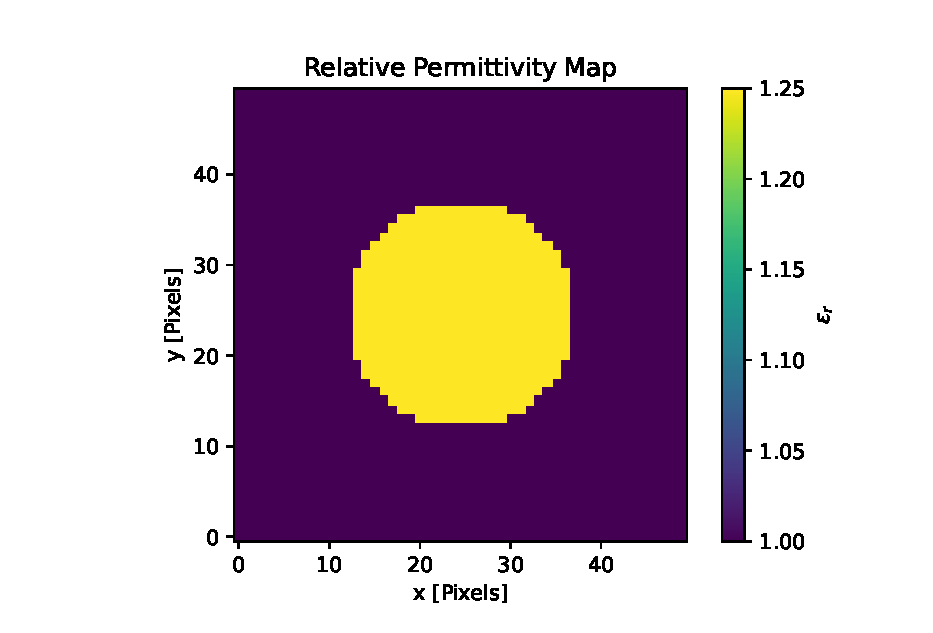
\includegraphics[width=.5\textwidth]{figuras/lcurve_input}}
					\subfloat[]{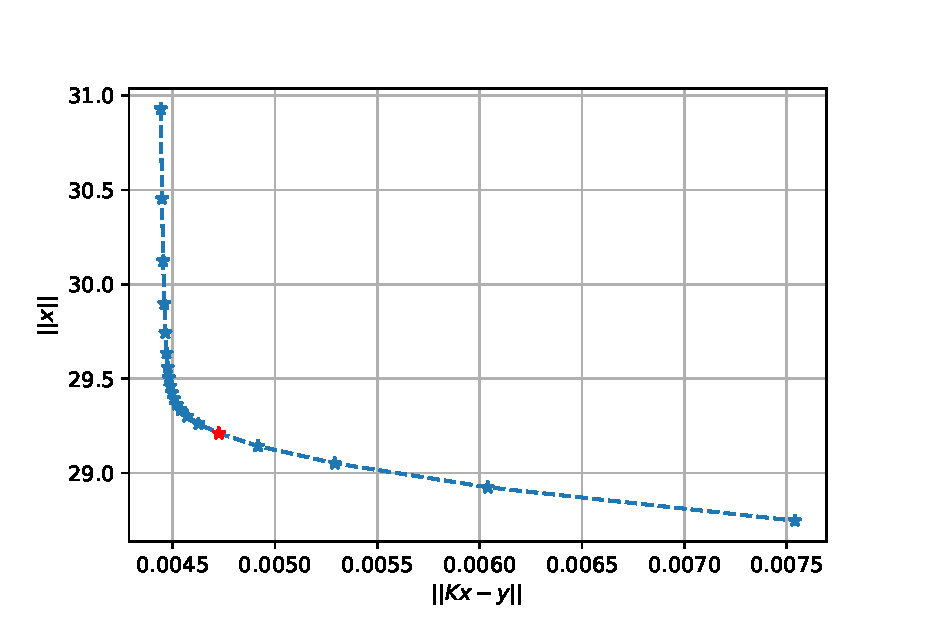
\includegraphics[width=.5\textwidth]{figuras/lcurve}} \\
					\subfloat[]{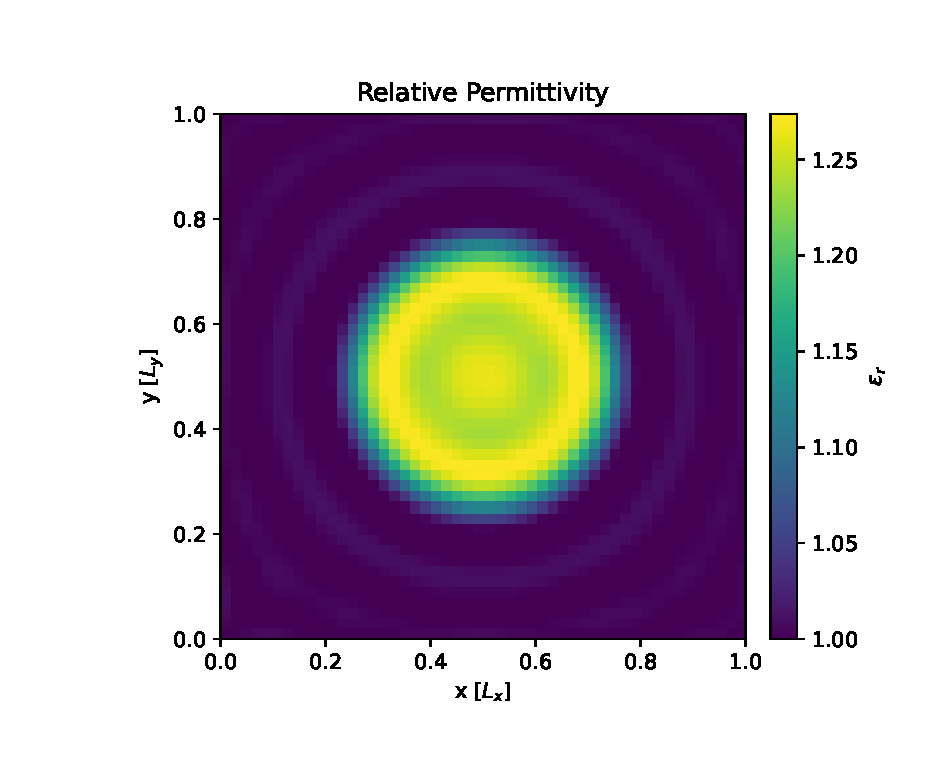
\includegraphics[width=.5\textwidth]{figuras/lcurve_result}}
					\caption[Exemplo de aplicação do Método da Curva-L.]{Example of applying the L-curve Method to a linear problem where it presupposes knowledge of the total field. (a) A simple instance of a contrast dielectric circle $\chi=0.25$ and radius $0.8\lambda_b$. Respecting the degrees of freedom, the scattered field was sampled in 45 positions for 45 incidence angles at a distance of $10\lambda_b$ from the center of the image. (b) L-curve considering 20 values of $\alpha_T$ in a range of $10^{-5}$ a $10^{-2}$. The red dot represents the solution with the shortest normalized distance to the origin. Its $\alpha_T$ value is approximately $2.3357 \times10^{-3}$. (c) Reconstruction of the image using the $\alpha_T$ value from the red dot. No inverse crime was committed since the data were obtained from the analytical solution.}
					\label{fig:3:lcurve}
				\end{figure}
				
			\subsubsection{Trial and Error}\label{chap:methods:linear:tikhonov:trialanderror}
				
				%Por fim, não poderíamos deixar de destacar a abordargem tentativa-e-erro no qual um conjunto de valores de $\alpha_T$ são testados para um problema canônico. A partir destes testes, escolhe-se o valor do resultado mais razoável de acordo com algum critério e utiliza-se esse valor para outros experimentos. Em muitas situações práticas não é necessário o esforço de obter o melhor valor. Basta apenas identificar um intervalo no qual qualquer valor escolhido produza resultados razoáveis. Assim, esta é uma estratégia \textit{a priori}, na qual o valor é definido na entrada do algoritmo.
				Finally, the trial-and-error approach is another popular strategy. A set of $\alpha_T$ values are tested for a canonical problem. The most reasonable result value is chosen according to some criterion, and this value is used for other experiments. In many practical situations, no effort is required to obtain the best value but only identifying a range in which any chosen value produces reasonable results. Therefore, this is \textit{a priori} strategy, in which the value is defined at the input of the algorithm. 
				
		\subsection{The Landweber Regularization}\label{chap:methods:linear:landweber}
				
			%É possível resolver o sistema $\mathcal{K}\{x\}=y$ de forma iterativa se escrevermos a solução $x$ na forma $x=(\mathcal{I}-\alpha_L\mathcal{K}^*\mathcal{K})x+ \alpha_L \mathcal{K}^*\{y\}$ para um $\alpha_L > 0$. Ou seja, a solução é computada iterativamente por:
			It is possible to solve the system $\mathcal{K}\{x\}=y$ iteratively if we write the solution $x$ in the form $x=(\mathcal{I}-\alpha_L\mathcal{K}^*\mathcal{K})x+ \alpha_L \mathcal{K}^*\{y\}$ for an $\alpha_L > 0$. That is, the solution is computed iteratively by:
			\begin{equation}
				x^m=(\mathcal{I}-\alpha_L\mathcal{K}^*\mathcal{K})x^{m-1}+ \alpha_L \mathcal{K}^*\{y\} \label{eq:3:linear:landweber:0}
			\end{equation}
		
			%\noindent cujo o chute inicial pode ser definido como $x^0\coloneqq 0$. Este esquema é semelhante a uma algoritmo de passo descendente no qual o funcional quadrático $||\mathcal{K}\{x\}-y||^2$ é minimizado. O operador de regularização equivalente à definição \eqref{eq:2:inverse:2} pode ser expresso nesse caso como:
			\noindent where the initial guess can be defined as $x^0\coloneqq 0$. This scheme is similar to a descent step algorithm in which the quadratic functional $||\mathcal{K}\{x\}-y||^2$ is minimized. The regularization operator equivalent to the definition \eqref{eq:2:inverse:2} can be expressed in this case as:
			\begin{equation}
				\mathcal{R}_L \coloneqq \alpha_T \sum\limits_{k=0}^{m-1} (\mathcal{I}-\alpha_L\mathcal{K}^*\mathcal{K})^k\mathcal{K}^*,~~ m=1,2,\cdots \label{eq:3:linear:landweber:operator}
			\end{equation}
			
			%No entanto, é necessário definir um critério de parada para o método. Se $\mathcal{K}:X\rightarrow Y$ é um operador linear, compacto e um-pra-um com intervalo denso, então a sequência $x^{m,\delta}$ de \eqref{eq:3:linear:landweber:0}, $m=0,1,2,\cdots$, pode ser rearranjada para:
			However, it is necessary to define a stopping criterion for the method. If $\mathcal{K}:X\rightarrow Y$ is a linear, compact, and one-to-one operator with a dense interval, then the sequence $x^{m,\delta}$ of \eqref{eq:3:linear:landweber:0}, m = $m=0,1,2,\cdots$, can be rearranged to:
			\begin{equation}
				x^{m+1,\delta} = x^{m,\delta} + \alpha_L\mathcal{K}^*\{y-\mathcal{K}\{x^{m,\delta}\}\},~~m=0,1,2,\cdots \label{eq:3:linear:landweber:1}
			\end{equation}
		
			%Dentro dessa definição, pressupõe-se que $||y-y^\delta||\le\delta$, $||y^\delta||\ge r\delta$ para um $r>1$, $\delta\in(0,\delta_0)$ e $0\le \alpha_L \le 1/||\mathcal{K}||^2$. Nestas condições, o critério de parada $||\mathcal{K}\{x^{m,\delta}\}-y^\delta||\le r\delta$ é bem definido, i.e., existe um $m=m(\delta) \in \mathbb{N}_0$ para o qual $||\mathcal{K}\{x^{m,\delta}\}-y^\delta||\le r\delta$. Além disso, é possível demonstrar que essa sequência converge para $x$ e que, se $x=\mathcal{K}^*\{z\}\in\mathcal{K}^*(Y)$ ou $x=\mathcal{K}^*\{\mathcal{K}\{z\}\}\in\mathcal{K}^*\mathcal{K}(X)$ para um $z$ tal que $||z||\le E$, então a ordem de convergência é expressa por \citep{kirsch2011introduction}:
			Within this definition, it is assumed that $||y-y^\delta||\le\delta$, $||y^\delta||\ge r\delta$ for an $r>1$, $\delta\in(0,\delta_0)$ and $0\le \alpha_L \le 1/||\mathcal{K}||^2$. Under these conditions, the stop criterion $||\mathcal{K}\{x^{m,\delta}\}-y^\delta||\le r\delta$ is well defined, i.e., there is a $m=m(\delta) \in \mathbb{N}_0$ for which $||\mathcal{K}\{x^{m,\delta}\}-y^\delta||\le r\delta$. In addition, it is possible to demonstrate that this sequence converges to $x$ and that, if $x=\mathcal{K}^*\{z\}\in\mathcal{K}^*(Y)$ or $x=\mathcal{K}^*\{\mathcal{K}\{z\}\}\in\mathcal{K}^*\mathcal{K}(X)$ for a $z$ such that $||z||\le \Delta$, then the convergence order is expressed by \citep{kirsch2011introduction}:
			\begin{align}
				||x^{m(\delta),\delta}-x|| &\le c\sqrt{\Delta\delta} \label{eq:3:linear:landweber:error1} \\
				||x^{m(\delta),\delta}-x|| &\le c\Delta^{1/3}\delta^{2/3} \label{eq:3:linear:landweber:error2}
			\end{align}
		
			%\noindent respectivamente, para um $c>0$. Em outras palavras, isto significa dizer que a escolha $m(\delta)$ é ótima.
			\noindent respectively, for a $c>0$. In other words, this means that the choice $m(\delta)$ is optimal.
			
			%O método pode ser aplicado no sistema $\mathbf{\bar{E}}^{\mathbf{s},F} = \mathbf{\bar{K}}\boldsymbol{\chi}$ conforme ilustrado no \autoref{alg:landweber}.
			The method can be applied in $\mathbf{\bar{E}}^{\mathbf{s},F} = \mathbf{\bar{K}}\boldsymbol{\chi}$ as illustrated in \autoref{alg:landweber}.
			\begin{algorithm}[!htb]
				\caption{Landweber Method.}
				\label{alg:landweber}
				\KwIn{$\mathbf{\bar{E}}^{\mathbf{s},F}$,$\mathbf{\bar{K}}$, $\alpha_L$, $\delta$}
				\KwOut{$\boldsymbol{\chi}^m$}
				$\boldsymbol{\chi}^0 \leftarrow \mathbf{0}$ \\
				$m\leftarrow 0$ \\
				\While {$||\mathbf{\bar{K}}\boldsymbol{\chi}^m-\mathbf{\bar{E}}^{\mathbf{s},F}|| \le \delta$} {
					$\boldsymbol{\chi}^{m+1} = \boldsymbol{\chi}^m + \alpha_T\mathbf{\bar{K}}^*\left(\mathbf{\bar{E}}^{\mathbf{s},F}-\mathbf{\bar{K}}\boldsymbol{\chi}^m\right)$ \\
					$m \leftarrow m + 1$ \\
				}
			\end{algorithm}
				
		\subsection{The Conjugate Gradient Method}\label{chap:methods:linear:cg}
				
			%O Método do Gradiente Conjugado (CG) é muito popular e aplicado a diversas situações. Nesta seção nos concentraremos na aplicação para problema inversos de equações com operadores limitados, lineares e injetivos entre espaços de Hilbert. Ou seja, dada equação $\mathcal{K}\{x\} = y$ no qual $\mathcal{K} : X \rightarrow Y$ tem as propriedades anteriores comentadas e a adjunta $\mathcal{K}^* : Y \rightarrow X$, definimos o funcional:
			The Conjugated Gradient Method (CG) is very popular and applied to several situations. This section will focus on its formulation for the inverse problem with integral equations considering bounded, linear, and injective operators between Hilbert spaces. Particularly, given equation $\mathcal{K}\{x\} = y$ in which $\mathcal{K} : X \rightarrow Y$ has the previous properties commented and the adjoint $\mathcal{K}^* : Y \rightarrow X$, we define the functional:
			\begin{equation}
				f(x) \coloneqq ||\mathcal{K}\{x\} - y||^2 = \langle \mathcal{K}\{x\} - y, \mathcal{K}\{x\} - y \rangle \label{eq:3:linear:cg:0}
			\end{equation}
		
			%O gradiente de \eqref{eq:3:linear:cg:0} é calculado pela representação de Riesz da derivada de Frechét de $f$, a qual é expressa por:
			The gradient of \eqref{eq:3:linear:cg:0} is calculated by the Riesz representation of the Frechét derivative, which is expressed by:
			\begin{equation}
				\nabla f(x) \coloneqq 2\mathcal{K}^*\{\mathcal{K}\{x\}-y\} \in X \label{eq:3:linear:cg:1}
			\end{equation}
		
			%Auxiliarmente, denominaremos dois elementos $p,q\in X$ como $\mathcal{K}$-conjugados se $\langle \mathcal{K}\{p\}, \mathcal{K}\{q\}=0$. Se $\mathcal{K}$ é um-pra-um, esta definição tem as mesmas propriedades do produto interno em $X$.
			Auxiliary, we will call two elements $p,q\in X$ as $\mathcal{K}$-conjugated if $\langle \mathcal{K}\{p\}, \mathcal{K}\{q\}=0$. If $\mathcal{K}$ is one-to-one, this definition has the same properties as an inner product in $X$.
			
			%A partir destas definições, podemos definir a sequência $x^m$ estabelecida para o CG como:
			From these definitions, we can define the sequence $x^m$ established for CG as:
			\begin{equation}
				x^{m+1} = x^m - t_mp^m \label{eq:3:linear:cg:2}
			\end{equation}
		
			\noindent where:
			\begin{align}
				t_m &= \langle \mathcal{K}\{x^m\}-y, \mathcal{K}\{p^m\} \rangle \label{eq:3:linear:cg:3} \\
				p^{m+1} &\coloneqq \mathcal{K}^*\{\mathcal{K}\{x^{m+1}\}-y\} + \gamma_m p^m \label{eq:3:linear:cg:4} \\
				\gamma_m &\coloneqq \frac{||\mathcal{K}^*\{\mathcal{K}\{x^{m+1}\}-y\}||^2}{||\mathcal{K}^*\{\mathcal{K}\{x^{m}\}-y\}||^2} \label{eq:3:linear:cg:5}
			\end{align}
		
			%Neste método, os gradientes das sequências de $x$ são ortogonais. Além disso, as sequências de direções $p$ são $\mathcal{K}$-conjugadas. Sob certas condições, este algoritmo convergiria para uma solução no qual $\mathcal{K}^*\{\mathcal{K}\{x^{m+1}\}-y\} = 0$. No entanto, quando só é conhecido um $y^\delta\in I$ tal que $||y^\delta-y||\le\delta$, então um critério de parada é o limiar $||\mathcal{K}\{x^{m,\delta}\}-y^\delta||\le\delta$.
			In this method, the gradients of the $x$ sequences are orthogonal. Furthermore, the sequences of directions $p$ are $\mathcal{K}$-conjugated. Under certain conditions, this algorithm converge to a solution in which $\mathcal{K}^*\{\mathcal{K}\{x^{m+1}\}-y\} = 0$. However, when only a $y^\delta\in I$ is known such that $||y^\delta-y||\le\delta$, then a stopping criterion is the threshold $||\mathcal{K}\{x^{m,\delta}\}-y^\delta||\le\delta$.
			
			%A aplicação deste método sobre a equação $\mathbf{\bar{E}}^{\mathbf{s},F}=\mathbf{\bar{K}}\boldsymbol{\chi}$ pode ser vista no \autoref{alg:cg}. Uma das vantagens é que este não depende de um parâmetro de regularização tal qual os métodos de Tikhonov e Landweber. No entanto, o método depende de mais operações.
			The application of this method on $\mathbf{\bar{E}}^{\mathbf{s},F}=\mathbf{\bar{K}}\boldsymbol{\chi}$ can be seen in \autoref{alg:cg}. One of the advantages is that it does not depend on a regularization parameter as Tikhonov and Landweber methods. However, the method depends on more operations.
			\begin{algorithm}[!htb]
				\caption{Conjugated Gradient Method.}
				\label{alg:cg}
				\KwIn{$\mathbf{\bar{E}}^{\mathbf{s},F}$,$\mathbf{\bar{K}}$, $\delta$}
				\KwOut{$\boldsymbol{\chi}^m$}
				$\mathbf{p}^0 \leftarrow -\mathbf{\bar{K}^*}\mathbf{\bar{E}}^{\mathbf{s},F}$ \\
				$\boldsymbol{\chi}^0 \leftarrow \mathbf{0}$ \\
				$m\leftarrow 0$ \\
				\While {$||\mathbf{\bar{K}^*}(\mathbf{\bar{K}}\boldsymbol{\chi}^m-\mathbf{\bar{E}}^{\mathbf{s},F})|| < \delta$} {
					$t_m = \frac{\left[\mathbf{\bar{K}}\boldsymbol{\chi}-\mathbf{\bar{E}}^{\mathbf{s},F}\right]^T\overline{\mathbf{\bar{K}}\mathbf{p}}}{||\mathbf{\bar{K}}\mathbf{p}||^2} $ \\
					$\boldsymbol{\chi}^{m+1} \leftarrow \boldsymbol{\chi}^m - t_m\mathbf{p}^m$ \\
					$\gamma_m = \frac{||\mathbf{\bar{K}^*}\left(\mathbf{\bar{K}}\boldsymbol{\chi}^{m+1}-\mathbf{\bar{E}}^{\mathbf{s},F})\right)||^2}{||\mathbf{\bar{K}^*}\left(\mathbf{\bar{K}}\boldsymbol{\chi}^m-\mathbf{\bar{E}}^{\mathbf{s},F}\right)||^2}$ \\
					$\mathbf{p}^{m+1} = \mathbf{\bar{K}^*}\left(\mathbf{\bar{K}}\boldsymbol{\chi}^{m+1}-\mathbf{\bar{E}}^{\mathbf{s},F}\right) + \gamma_m \mathbf{p}^m$ \\
					$m \leftarrow m + 1$ \\
				}
			\end{algorithm}
				
		\subsection{Spectral Cut-Off}\label{chap:methods:linear:spectral}
					
			%Uma vez que o problema é mal-posto, $\mathbf{\bar{K}}$ é uma matriz cujos os autovalores se aproximam de zero. Quando aplica-se a Decomposição por Valor Singular (SVD) em $\mathbf{\bar{K}}$, o seguinte produto é obtido:
			Since the problem is ill-posed, $\mathbf{\bar{K}}$ is a matrix whose eigenvalues approach zero. When the Single Value Decomposition (SVD) is applied in $\mathbf{\bar{K}}$, the following product is obtained:
			\begin{equation}
				\mathbf{\bar{K}} = \mathbf{\bar{U}}\boldsymbol{\bar{\xi}}\mathbf{\bar{V}}^* \label{eq:3:linear:spectral:0}
			\end{equation}
		
			%\noindent no qual $\mathbf{\bar{U}}$ é uma matriz $N_MN_S\times N_MN_S$ composta por vetores singulares $\mathbf{u}_m$ os quais são ortogonais e unitários; $\mathbf{\bar{V}}$ é uma matriz $N_IN_J\times N_IN_J$ composta por vetores singulares $\mathbf{v}_m$ os quais também são ortogonais e unitários; e $\boldsymbol{\bar{\xi}}$ é a matriz diagonal composta pelos valores singulares $\xi_i$ os quais são reais e em ordem decrescente $\xi_1\ge\xi_2\ge\cdots\ge0$. Matematicamente, a solução $\boldsymbol{\chi}$ pode ser escrita como:
			\noindent in which $\mathbf{\bar{U}}$ is a matrix $N_MN_S\times N_MN_S$ composed of singular vectors $\mathbf{u}_m$ 's which are orthogonal and unitary; $\mathbf{\bar{V}}$ is an $N_IN_J\times N_IN_J$ matrix composed of singular vectors $\mathbf{v}_m$'s which are also orthogonal and unitary; and $\boldsymbol{\bar{\xi}}$ is the diagonal matrix composed of the singular values $\xi_i$'s which are real and place in nonincreasing order  $\xi_1\ge\xi_2\ge\cdots\ge0$. Mathematically, the solution $\boldsymbol{\chi}$ can be written as:
			\begin{equation}
				\boldsymbol{\chi} = \mathbf{\bar{K}}^{-1}\mathbf{\bar{E}}^{\mathbf{s},F} = \sum\limits_{\xi_i\neq0} \frac{1}{\xi_i} \left(\mathbf{u}^*_i\cdot\mathbf{\bar{E}}^{\mathbf{s},F}\right)\mathbf{v}_i \label{eq:3:linear:spectral:1}
			\end{equation}
			
			%Uma vez que $\boldsymbol{\bar{\xi}}$ contém autovalores próximo ou iguais a zero, a operação \eqref{eq:3:linear:spectral:1} é inviável porque pode levar a erros numéricos muito grandes. Isto equivale a dizer que a inversa de $\mathbf{\bar{K}}$ é não-limitada. Por isso, uma alternativa é excluir autovalores menores que um limiar, i.e., $\xi_i<\alpha_{S}$. Assim, \eqref{eq:3:linear:spectral:1} pode ser escrita como um operador de regularização $\mathcal{R}_{SC}$ como:
			Once $\boldsymbol{\bar{\xi}}$ contains eigenvalues close or equal to zero, the operation \eqref{eq:3:linear:spectral:1} is not feasible since it can lead to substantial numerical errors. This is equivalent to saying that the inverse of $\mathbf{\bar{K}}$ is unbounded. Therefore, an alternative is to exclude eigenvalues smaller than a threshold, i.e., $\xi_i<\alpha_{S}$. Then, \eqref{eq:3:linear:spectral:1} can be written as an operator regularization $\mathcal{R}_{SC}$ as:
			\begin{equation}
					\boldsymbol{\chi} = \mathcal{R}_{SC}\{\mathbf{\bar{E}}^{\mathbf{s},F}\} = \sum\limits_{\xi_i>\alpha_{S}} \frac{1}{\xi_i} \left(\mathbf{u}^*_i\cdot\mathbf{\bar{E}}^{\mathbf{s},F}\right)\mathbf{v}_i \label{eq:3:linear:spectral:2}
			\end{equation}
		
			%Este método de regularização é chamado de Corte Espectral e depende da definição de um parâmetro de corte $\alpha_{S}$. Esta solução também conhecida como Norma Mínima. Este método é adequado quando a dimensão das matrizes não são tão grandes, uma vez que o custo computacional para o cálculo dos autovalores e autovetores é elevado. No entanto, o método é muito útil para classificar problemas mal-postos: problemas cujos os autovalores decaem a zero de maneira suave são chamados problemas mildly mal-postos; problemas cujos os autovalores decaem rapidamente a zero são chamados problemas severamente mal-postos.
			This regularization method is called the Spectral Cut-Off and depends on setting a cutting parameter $\alpha_{S}$. This solution is also known as Minimum Norm. This method is suitable when the size of the matrices is not too large since the computational cost for evaluating eigenvectors and eigenvalues may be high. However, the method is convenient for classifying ill-posed problems. The reason is: problems whose eigenvalues drop to zero smoothly are called mildly ill-posed; problems whose eigenvalues rapidly decay to zero are called severely ill-posed problems.
	
	\section{Qualitative Methods}\label{chap:methods:qualitative}
			
		When the contrast estimation is not a required information, qualitative methods are more efficient as they retrieve information about shape and position of scatterers with less computational effort. Even though applications that do not require electric property retrieval seem to be rare, qualitative methods might provide initial solutions for quantitative ones. In the next subsections, some of the qualitative methods are discussed. For a survey of them, readers are referred to \citep{potthast2006survey}.
		
		\subsection{Linear Sampling Method}\label{chap:methods:qualitative:lsm}
			
			The Linear Sampling Method (LSM) is a fast and traditional qualitative method \citep{colton2019inverse,colton1996simple}. If plane waves propagate through the space and the scattered field is sampled in far field conditions, then the scattered field admits the asymptotic behavior given by:
			\begin{equation}
				E_{s_z}(\rho, \theta, \phi) = \frac{e^{-jk_b\rho}}{\sqrt{\rho}}E_{s_\infty}(\theta, \phi) \label{eq:3:qualitative:lsm:kernel}
			\end{equation}
		
			\noindent where $E_{s_\infty}(\theta, \phi)$ is the far-field pattern of the scattered field. For any point $\boldsymbol{\rho}$ in $S$, the following far-field integral holds:
			\begin{equation}
				\int_D d\phi E_{s_\infty}(\theta, \phi) g(\boldsymbol{\rho}, \phi) = \Phi_\infty(\theta, \boldsymbol{\rho}) \label{eq:3:qualitative:lsm:integralequation}
			\end{equation}
		
			\noindent where $\Phi_\infty(\theta, \boldsymbol{\rho})$ is the far-field pattern of the Green's function $-(jk_b^2/4)G^D_{2D}(\theta,\boldsymbol{\rho})$ when the source point is at $\boldsymbol{\rho}$ and the observation point is in the direction $\theta$. $\Phi_\infty(\theta, \boldsymbol{\rho})$ is a function that might be approximated by:
			\begin{equation}
				\Phi_\infty(\theta, \boldsymbol{\rho}) \approx \frac{-j}{4}\sqrt{\frac{2}{\pi k_b}}e^{j\pi/4}e^{jk_b\cos(\theta-\psi)}  \label{eq:3:qualitative:lsm:rhs}
			\end{equation}
		
			\noindent where $\boldsymbol{\rho} = \langle x, y \rangle =  \langle \rho\cos(\psi), \rho\sin(\psi)\rangle$.
			
			The idea behind LSM is to choose an indicator function defined in $S$ which determines if a spatial point belongs or not to a scatterer. The integral equation \eqref{eq:3:qualitative:lsm:integralequation} is solved for $g(\boldsymbol{\rho}, \phi)$ for each $\boldsymbol{\rho}$ in $S$ and each $\phi$ in $D$. The integral equation might be solved through a regularization method (Section \ref{chap:methods:regularization}) after computing the kernel in \eqref{eq:3:qualitative:lsm:integralequation} by \eqref{eq:3:qualitative:lsm:kernel} based on the scattered field data and the right-hand-side \eqref{eq:3:qualitative:lsm:rhs}. The indicator function $I(\boldsymbol{\rho})$ is defined as:
			\begin{equation}
				I(\boldsymbol{\rho}) = ||g(\boldsymbol{\rho})|| = \sqrt{\int_D d\theta |g(\boldsymbol{\rho})|^2} \label{eq:3:qualitative:lsm:indicator}
			\end{equation}
		
			The value indicator function becomes unbound if $\boldsymbol{\rho}$ is not within a scatterer region \citep{colton1996simple}. Therefore, after computing $I(\boldsymbol{\rho})$ for many points in $S$, we are able to recover the scatterer image by verifying if $I(\boldsymbol{\rho})$ tends to infinite or not. Due to discretization of $D$ and $S$ and noise presence in the scattered field data, $I(\boldsymbol{\rho})$ cannot be infinite. Therefore is necessary to set a threshold heuristically for which the background will be set apart from the scatterer.
			
			The LSM is not limited to far-field data. For near-field data, the integral equation \eqref{eq:3:qualitative:lsm:integralequation} is replaced by \citep{cakoni2016qualitative}:
			\begin{equation}
				\int_D d\phi E_{s_z}(\theta, \phi) g(\boldsymbol{\rho}, \phi) = - \frac{jk_b^2}{4} G^D_{2D}(\theta,\boldsymbol{\rho}) \label{eq:3:qualitative:lsm:nearfield}
			\end{equation}
		
			The LSM cannot estimate the dielectric properties of the media. However, it might help the performance of other inversion methods \citep{catapano2007simple,bao2007inverse} and some approximations might be done to turn it into a quantitative method \citep{crocco2012linear}. Further discussion may be found in \citep[see][chap. 5]{chen2017}, \citep{cakoni2016qualitative} and \citep[see][chap. 5]{pastorino2010}.
		
		\subsection{Orthogonality Sampling Method}\label{chap:methods:qualitative:osm}
		
			The Orthogonality Sampling Method (OSM) is another approach to define an indicator function which detects the presence of scatterers \citep{potthast2010study}. Instead of writing it in terms of the solution of the integral equation \eqref{eq:3:qualitative:lsm:integralequation}, the orthogonality between far-field data and an exponential function is tested. Another interpretation is the superposition of plane waves back into the region of the scatterer, which is a very known idea. Mathematically, the orthogonality is tested according to \citep{potthast2010study,akinci2016nearfield}:
			\begin{equation}
				E_{s_z}^{red} (\boldsymbol{\rho}, \theta) = \int_D d\phi E_{s_\infty}(\theta,\phi)e^{-jk_b\rho\cos(\theta-\psi)} = \int_D d\phi \frac{e^{-jk_b/4}}{\sqrt{8\pi k_b}} E_{s_z}(\theta, \phi) e^{-jk_b\rho\cos(\theta-\psi)} \label{eq:3:qualitative:osm:farfield:equation}
			\end{equation}
		
			\noindent where $E_{s_z}^{red}$ is know as the reduced scattered field. The indicator function is defined as:
			\begin{equation}
				I(\boldsymbol{\rho}) = \int_D d\theta |E_{s_z}^{red} (\boldsymbol{\rho}, \theta)|^2 \label{eq:3:qualitative:osm:farfield:indicator}
			\end{equation}
		
			Therefore, the indicator function computation does not require solving an integral equation. Rather it depends on integrating reduced scattered field. The maxima of the function is used to identify the scatterers. Near-field data is also compatible with the method. However, the reduced scattered field definition needs to be adapted \citep{akinci2016nearfield}:
			\begin{equation}
				E_{s_z}^{red} (\boldsymbol{\rho}, \theta) = = \int_D d\phi E_{s_z}(\theta, \phi) K^{TM}(\theta, \boldsymbol{\rho}) \label{eq:3:qualitative:osm:nearfield:equation}
			\end{equation}
		
			\noindent where:
			\begin{equation}
				K^{TM}(\theta, \boldsymbol{\rho}) = \frac{-2j}{\pi R_O}\sum\limits_{n=-\infty}^{\infty} \frac{J_n(k_b\rho)}{H_n^{(2)}(k_bR_O)}e^{-jn(\theta-\psi)} \label{eq:3:qualitative:osm:nearfield:indicator}
			\end{equation}
		
			\cite{akinci2016nearfield} stated that the reduced scattered field is directly related to the electrical properties of the scatterers. \cite{bevacqua2020physical} went further and concluded that the reduced scattered field can be related to the radiating component of the induced currents. As a consequence, OSM is able to image discontinuities within unknown scatterers and identify regions with different electromagnetic properties, differently than other qualitative methods.
			
	\section{Deterministic Quantitative Methods}\label{chap:methods:deterministic}
			
		%Considerando agora o problema não-linear, existe uma classe de métodos que resolvem as equações de forma determinística, i.e., sem o recurso de operações aleatórias. Esta classe é a mais popular na literatura do problema, a qual possui uma grande quantidade de métodos. Nesta seção serão discutidos tanto métodos tradicionais que foram relevantes na história da literatura quanto aqueles que são considerados estado-da-arte.
		Now considering the nonlinear and quantitative problem, there is a class of methods that solve the equations in a deterministic fashion, i.e., without the use of random operations. This class is the most popular in the problem literature, which has a large number of methods. This section will discuss both traditional methods relevant to the history of literature and those that are considered state-of-the-art.
				
		\subsection{The Born Iterative Method}\label{chap:methods:deterministic:bim}
					
			%Um dos primeiros métodos a se popularizar foi proposto por \cite{wang1989iterative}. Pressupondo que o meio de fundo é conhecido e homogêneo, os autores proporam uma abordagem iterativa onde cada iteração era equivalente à solução por séries de Neumann. A partir de uma estimativa inicial da função contraste, o processo iterativo se baseia em obter uma solução para o campo total através de um resolvedor direto e resolver o problema linear inverso a partir desta estimativa do campo para atualizar a estimativa da função contraste (\autoref{alg:bim}). Portanto, o método se baseia em uma estratégia de linearização do problema, i.e., dividindo o problema em subproblemas lineares.
			One of the first methods to become popular was proposed by \cite{wang1989iterative}. Assuming a homogeneous background medium, the authors proposed an iterative approach where each iteration was equivalent to the solution by Neumann series. From an initial estimate of the contrast function, the iterative process is based on obtaining a solution for the total field through a direct solver and solving the inverse linear problem to update the estimate of the contrast function based on the current estimate of the total field (\autoref{alg:bim}). Therefore, the method is based on a linearization strategy, i.e., dividing the problem into two linear subproblems.
			
			\begin{algorithm}[!htb]
				\caption{Born Iterative Method.}
				\label{alg:bim}
				\KwIn{$\mathbf{\bar{E}^s}$, $\mathbf{\bar{E}^i}$, $\mathbf{\bar{G}^D}$, $\mathbf{\bar{G}^S}$}
				\KwOut{$\boldsymbol{\bar{\chi}}$, $\mathbf{\bar{E}}$}
				Compute an initial guess $\boldsymbol{\bar{\chi}^0}$ based on available information \\
				$m\leftarrow0$ \\
				\While{some criterion is not reached} {
					Update $\mathbf{\bar{E}}^m$ based on the current $\boldsymbol{\bar{\chi}}^m$ estimation \\
					Update $\boldsymbol{\bar{\chi}}^m$ based on the current $\mathbf{\bar{E}}^m$ estimation \\
				}
			\end{algorithm}
		
			%Originalmente, os autores utilizaram o Método dos Momentos definido por \cite{richmond1965scattering} como resolvedor direto e a Regularização de Tikhonov com parâmetro escolhido por tentativa-e-erro como resolvedor inverso. No entanto, outros resolvedores podem ser utilizados de forma que o método se tornou uma estrutura genérica onde muitas estratégias podem ser definidas, como por exemplo, os outros regularizadores definidos na seção anterior, o uso de funções de Conjunto de Nível \citep{shah2018fast} e Programação Quadrática \citep{batista2021quadratic}. Esta última técnica pode ser adequada para acoplar diferentes formas de regularização através da formulação da função objetivo.
			Initially, the authors used the Method of Moments defined by Richmond (1965) as the forward solver and Tikhonov's Regularization with a parameter chosen by trial-and-error as an inverse solver. However, other solvers can be used in such a way that the method has become a generic structure where many strategies can be defined, for example, the other regularizers defined in the previous section, the use of Level Set functions \citep{shah2018fast} and Quadratic Programming \citep{batista2021quadratic}. This latter technique may be suitable for coupling different forms of regularization through the objective function definition.
			
			%No artigo original, os autores chamaram o algoritmo de Método de Newton Modificado, uma vez que o processo iterativo pode ser comparado com a definição de uma direção busca para uma solução corrente. No entanto, o algoritmo ficou conhecido na literatura como Método Iterativo de Born (BIM) uma vez que o objetivo era propor uma solução para os casos onde a Aproximação de Born não era válida. Embora a intenção fosse essa, o algoritmo também tem limites em relação à aplicação em casos de alto contraste. Geralmente, a solução inicial é determinada pela Aproximação de Born, e por isso, a convergência do algoritmo pode ficar comprometida em situações de espalhadores fortes. \cite{moghaddam1993study} se aprofundou nesta questão mostrando boas reconstruções para objetos com diâmetro de $8.5\lambda_b$ em relação à frequência central de operação\footnote{Neste trabalho, os autores formularam o problema no domínio do tempo. Este tipo de formulação tem a vantagem de considerar mais frequências no processo de inversão.} e contraste $\chi=1$. No entanto, não existe na literatura uma medição robusta sobre a relação entre contraste e tamanho que o BIM é capaz de suportar. Destaca-se também a comparação entre o BIM e Método de Tarantola realizada por \cite{moghaddam1991comparison} no qual concluiu-se que, embora o Método de Tarantola tenha um custo computacional menor do que o BIM, este último pode convergir mais rápido e ser mais robusto com objetos que têm pontas.
			In the original article, the authors called the Modified Newton Method algorithm since the iterative process can be compared with the definition of a search direction for a current solution. However, the algorithm was known in the literature as the Born Iterative Method (BIM) since the objective was to propose a solution for cases where the Born Approximation was not valid. Although this was the intention, the algorithm also has limits concerning the application in cases of high contrast. Generally, the initial solution is determined by the Born Approximation, and therefore, the convergence of the algorithm can be compromised when strong scatterers are considered. \cite{moghaddam1993study} went deeper into this issue showing good reconstructions for objects with a diameter of $8.5\lambda_b$ in relation to the central frequency of operation\footnote{In this work, the authors formulated the problem in the time domain. This type of formulation has the advantage of considering more frequencies in the inversion process.} and contrast $\chi=1$. However, there is no robust measurement in the literature on the relationship between contrast and size that BIM can support. Also noteworthy is the comparison between BIM and the Tarantola Method carried out by \cite{moghaddam1991comparison}. Although Tarantola's Method has a lower computational cost than BIM, the latter can converge faster and be more robust with objects that have edges.
			
			%É necessário destacar também que implementações do BIM as quais utilizam regularizadores baseados em parâmetros precisam de estratégias para a escolha do seu valor. Assim como no artigo original, muitos outros trabalhos na literatura os quais utilizam este tipo de regularizador na linearização do problema inverso, escolhem um valor fixo para todas as iterações baseados em tentativa-e-erro \citep{chew1995frequency,yao1997frequency,li2004three,chew1994inversion,batista2021quadratic}. De fato, a escolha não é trivial e não há uma regra simples para a escolha ótima no problema não-linear \citep{engl1988convergence}.
			It is also necessary to highlight that BIM implementations that use parameter-based regularizers need strategies to choose their value. As in the original article, many other works in the literature that use this kind of regularizer choose a fixed value for all iterations based on trial-and-error strategy \citep{chew1995frequency,yao1997frequency,li2004three,chew1994inversion,batista2021quadratic}. In fact, the choice is not trivial, and there is no simple rule for the optimal choice in the nonlinear problem \citep{engl1988convergence}.
			
			%No entanto, existem estratégias para uma definição dinâmica de $\alpha_T$ ao longo processo iterativo do BIM. No trabalho original, os autores afirmam que valores altos $\alpha_T$ são importantes para evitar componentes de alta frequência na função contraste a qual estão associadas com ruídos na imagem. No entanto, essa componentes também podem ser importantes para a reconstruções vértices do objeto. Conforme defendido por \cite{moghaddam1992nonlinear}, os pequenos autovalores em $\mathbf{\bar{K}}$ podem contribuir para uma melhor reconstrução dos contornos quando a função contraste já estiver suficientemente suave durante o processo de reconstrução. Por isso eles propõem que, nas primeiras iterações do BIM, sejam utilizados valores altos de $\alpha_T$ para filtrar variações bruscas na função contraste; a partir daí, $\alpha_T$ seria diminuído para melhorar os contornos da imagem. Conforme explicam, esta estratégia é equivalente a começar procurando soluções num subespaço menor e ir expandindo ao longo das iterações. Também foram propostas na literatura regras para esta adaptação de $\alpha_T$ \citep{lavarello2008study,joachimowicz1991inverse,franchois1997microwave,zaiping2000variational}. Semelhantemente, metodologias que consideram os dados do campo espalhado em múltiplas frequências sugerem um uso dinâmico similar, i.e., começar com as frequências mais baixas e terminar com as mais altas \citep{chew1995frequency,batista2021quadratic}.
			However, there are strategies for a dynamic definition of $\alpha_T$ throughout the iterative process. In the original work, the authors state that high $\alpha_T$ values are essential to avoid high-spatial-frequency components in the contrast function associated with noise in the image. However, these components can also be necessary for the object's vertex reconstructions. As advocated by \cite{moghaddam1992nonlinear}, the small eigenvalues in $\mathbf{\bar{K}}$ can better reconstruct the contours when the contrast function is already sufficiently smooth during the reconstruction process. For this reason, they propose that, in the first BIM iterations, high values of $\alpha_T$ should be used to filter out sudden variations in the contrast function; after that, $\alpha_T$ would be decreased to improve the contours of the image. As they explain, this strategy is equivalent to start looking for solutions in a smaller subspace and expanding over iterations. Rules for this adaptation of $\alpha_T$ have also been proposed in the literature \citep{lavarello2008study,joachimowicz1991inverse,franchois1997microwave,zaiping2000variational}. Similarly, methodologies that consider scattered field data with multiple frequencies suggest a similar dynamic use, i.e., starting with the lowest frequencies and ending with the highest ones \citep{chew1995frequency,batista2021quadratic}.
							
		\subsection{The Distorted Born Iterative Method}\label{chap:methods:deterministic:dbim}
				
			%Os mesmos autores do BIM também publicaram no ano seguinte uma metodologia alternativa \citep{chew1990reconstruction}. Nessa nova abordagem, as equações do subproblema inverso não são resolvidas para $\chi$, e sim, para uma variação $\Delta\chi$. Desta forma, a função contraste é atualizada a cada iteração $t$ pela forma $\chi^t = \chi^{t-1} + \Delta\chi$. No entanto, para resolver o subproblema inverso em função de $\Delta\chi$ é necessário resolver a equação integral considerando um meio de fundo não-homogêneo conforme \eqref{eq:app:green:28}. Por isso, a cada iteração, a função de Green para o meio não-homogêneo \eqref{eq:app:green:29} precisa ser calculada levando a estimativa do contraste do final da iteração anterior como meio de fundo.
			The same BIM authors also published an alternative methodology the following year \citep{chew1990reconstruction}. In this new approach, the inverse subproblem equations are not solved for $\chi$ but a variation $\Delta\chi$. Consequently, the contrast function is updated at each iteration $t$ by the form $\chi^t = \chi^{t-1} + \Delta\chi$. However, to solve the inverse subproblem as a function of $\Delta\chi$, it is necessary to solve the integral equation considering a inhomogeneous background medium according to \eqref{eq:app:green:28}. Therefore, at each iteration, Green's function for the inhomogeneous medium \eqref{eq:app:green:29} needs to be calculated, taking the contrast estimate at the end of the previous iteration as the background medium.
					
			%Para calcularmos a função de Green não-homogênea em um problema bidimensional para um par de pontos $\brho_{m}$ e $\brho_{n}$, é necessário considerarmos a seguinte equação:
			The following equation must be considered for calculating the inhomogeneous Green function in a two-dimensional problem for a pair of points $\brho_{m}$ e $\brho_{n}$:
			\begin{equation}
				G_{in}(\brho_{m},\brho_{n}) = G_{2D}(\brho_{m},\brho_{n}) - \frac{jk_0^2}{4} \int_{S}dS^{\prime}~ G_{2D}(\brho_m,\brhop)\chi(\brhop)G_{in}(\brhop,\brho_n) \label{eq:3:deterministic:dbim:0}
			\end{equation}
				
			%\noindent onde $G_{2D}(\brho_{m},\brho_{n})=H^{(2)}_0(k_0|\brho_m-\brho_n|)$. Pelo teorema da reciprocidade, podemos reescrever \eqref{eq:3:deterministic:dbim:0} como:
			\noindent where $G_{2D}(\brho_{m},\brho_{n})=H^{(2)}_0(k_0|\brho_m-\brho_n|)$. By the reciprocity theorem, we can rewrite \eqref{eq:3:deterministic:dbim:0} as:
			\begin{equation}
				G_{in}(\brho_{n},\brho_{m}) = G_{2D}(\brho_{n},\brho_{m}) - \frac{jk_0^2}{4} \int_{S}dS^{\prime}~ G_{2D}(\brho_n,\brhop)\chi(\brhop)G_{in}(\brhop,\brho_m) \label{eq:3:deterministic:dbim:1}
			\end{equation}
		
			%Seguindo a mesma discretização de \eqref{eq:3:discretization:collocation:3}-\eqref{eq:3:discretization:collocation:7}, a região $S$ será dividida em $N_IN_J$ elementos e o valor de $G_{in}$ será amostrado nestes pontos:
			Following the same discretization of \eqref{eq:3:discretization:collocation:3}-\eqref{eq:3:discretization:collocation:7}, the $S$ region will be divided into $N_IN_J$ elements, and the value of $G_{in}$ will be sampled at these points:
			\begin{equation}
				G_{in}(\brho_{n},\brho_{m}) = G_{2D}(\brho_{n},\brho_{m}) - \sum\limits_{p=1}^{N_I}\sum\limits_{q=1}^{N_J} \chi(\brho_{pq}) G_{in}(\brho_{pq},\brho_{m}) \left(\frac{jk_0^2}{4}\int_{S_k}dS^{\prime}~ G_{2D}(\brho_n,\brhop)\right) \label{eq:3:deterministic:dbim:2}
			\end{equation}
		
			%Note que a integral entre parênteses é equivalente a \eqref{eq:3:discretization:collocation:1}. Por isso, ela pode ser substituída como foi feito em \eqref{eq:3:discretization:collocation:9}. Por isso, \eqref{eq:3:deterministic:dbim:2} pode ser escrita como um sistema de equações lineares:
			Note that the integral in parentheses is equivalent to  \eqref{eq:3:discretization:collocation:1}. So it can be replaced as was done in \eqref{eq:3:discretization:collocation:9}. Therefore, \eqref{eq:3:deterministic:dbim:2} can be written as a system of linear equations:
			\begin{equation}
				G^{in}_{nm} = G^{2D}_{nm} - \sum\limits_{p=1}^{N_I}\sum\limits_{q=1}^{N_J} \chi_{pq}G^{in}_{pqm} G^{2D}_{npq} \label{eq:3:deterministic:dbim:3}
			\end{equation}
		
			%\noindent no qual $G^{in}_{nm} = G_{in}(\brho_{n},\brho_{m})$, $G^{2D}_{nm}=G_{2D}(\brho_{n},\brho_{m}) $, $\chi_{pq}=\chi(\brho_{pq})$, $G^{in}_{pqm}=G_{in}(\brho_{pq},\brho_{m})$ e $G^{2D}_{npq}$ é o equivalente a \eqref{eq:3:discretization:collocation:1}.
			\noindent in which $G^{in}_{nm} = G_{in}(\brho_{n},\brho_{m})$, $G^{2D}_{nm}=G_{2D}(\brho_{n},\brho_{m}) $, $\chi_{pq}=\chi(\brho_{pq})$, $G^{in}_{pqm}=G_{in}(\brho_{pq},\brho_{m})$ and $G^{2D}_{npq}$ is equivalent to \eqref{eq:3:discretization:collocation:1}.
			
			%O objetivo é determinar a função de Green não-homogênea $G^{in}$ para que essa substitua $G^D_{2D}$ em \eqref{eq:3:definition:4}. Portanto, $\brho_m$ é um ponto de medição do campo em $D$. Já $\brho_n$ é um ponto da discretização em $S$. Por isso, \eqref{eq:3:deterministic:dbim:3} deve ser reescrita como:
			The objective is to determine the inhomogeneous Green function $G^{in}$ so that this replaces $G^D_{2D}$ in \eqref{eq:3:definition:4}. Therefore, $\brho_m$ is a measurement point of the field in $D$. Now $\brho_n$ is a point of discretization in $S$. Therefore, \eqref{eq:3:deterministic:dbim:3} should be rewritten as:
			\begin{equation}
				G^{in}_{mij} = G^{2D}_{mij} - \sum\limits_{p=1}^{N_I}\sum\limits_{q=1}^{N_J} \chi_{pq}G^{in}_{mpq} G^{S}_{ijpq} \label{eq:3:deterministic:dbim:4}
			\end{equation}
		
			%\noindent no qual $G^{in}_{mij} = G_{in}(\theta_m,x_i,y_j)$, $G^{2D}_{mij}$ é o mesmo que \eqref{eq:3:definition:9} para $\theta_m$, $x_i$, $y_j$; $\chi_{pq}=\chi(x_p, y_q)$ e $G^{S}_{npq}$ é o mesmo de \eqref{eq:3:discretization:collocation:9}. Desta forma, \eqref{eq:3:deterministic:dbim:4} pode ser escrita em forma matricial:
			\noindent where $G^{in}_{mij} = G_{in}(\theta_m,x_i,y_j)$, $G^{2D}_{mij}$ is the same of \eqref{eq:3:definition:9} for $\theta_m$, $x_i$, $y_j$; $\chi_{pq}=\chi(x_p, y_q)$ and $G^{S}_{npq}$ is equivalent to \eqref{eq:3:discretization:collocation:9}. Consequently, \eqref{eq:3:deterministic:dbim:4} might be rewrite in a matrix fashion:
			\begin{equation}
				\left(\mathbf{\bar{I}} - \mathbf{\bar{G}^S}\boldsymbol{\bar{\chi}}\right)\mathbf{\bar{G}^{in}} = \mathbf{\bar{G}^{2D}} \label{eq:3:deterministic:dbim:5}
			\end{equation}
		
			%\noindent no qual as matrizes $\mathbf{\bar{G}^{in}}$ e $\mathbf{\bar{G}^{2D}} $ são definidas de maneira similar a $\mathbf{\bar{G}^D}$. \eqref{eq:3:deterministic:dbim:5} pode ser resolvida a partir de técnicas para solução de sistemas lineares se transformarmos $\mathbf{\bar{G}^{in}}$ e $\mathbf{\bar{G}^{2D}}$ em vetores-coluna.
			\noindent in which the matrices $\mathbf{\bar{G}^{in}}$ and $\mathbf{\bar{G}^{2D}} $ are defined similarly to $\mathbf{\bar{G}^D}$. \eqref{eq:3:deterministic:dbim:5} can be solved using techniques for solving linear systems if we transform $\mathbf{\bar{G}^{in}}$ e $\mathbf{\bar{G}^{2D}}$ in column-vectors.
			
			%Portanto, o método proposto por \cite{chew1990reconstruction} precisa resolver \eqref{eq:3:deterministic:dbim:5} a cada iteração substituindo a matriz $\boldsymbol{\bar{\chi}}$ pela solução da função contraste obtida no final da iteração anterior. Convém destacar que muitos resolvedores diretos já utilizam a matriz $(\mathbf{\bar{I}} - \mathbf{\bar{G}^S}\boldsymbol{\bar{\chi}})$ em suas formulações, tal como o Método dos Momentos \citep{richmond1965scattering}. Além disso, é preciso levar em consideração os dados do campo espalhado em cada iteração. Uma vez que a equação integral deve ser resolvida para $\Delta\chi$, o campo espalhado na esquerda de \eqref{eq:3:discretization:collocation:10} de ser subtraído pela estimativa atual feita no resolvedor direto. Ou seja, o resolvedor direto calcula o campo total $\mathbf{\bar{E}}^t$ e o espalhado correspondente $\mathbf{\bar{E}}^{\mathbf{s},t}$. Desta forma, o resolvedor inverso determina $\Delta\chi$ a partir de $\mathbf{\bar{E}}^t$, $\mathbf{\bar{G}}^{\mathbf{in},t}$ e $\Delta\mathbf{\bar{E}^s} = \mathbf{\bar{E}^s} - \mathbf{\bar{E}}^{\mathbf{s},t}$.
			Therefore, the method proposed by \cite{chew1990reconstruction} needs to solve \eqref{eq:3:deterministic:dbim:5} at each iteration, replacing the $\boldsymbol{\bar{\chi}}$ matrix with the solution of the contrast function obtained at the end of the previous iteration. It should be noted that many forward solvers already use the matrix $(\mathbf{\bar{I}} - \mathbf{\bar{G}^S}\boldsymbol{\bar{\chi}})$ in their formulations, such as the Method of Moments \citep{richmond1965scattering}. In addition, it is necessary to take into account the scattered field data in each iteration. Since the integral equation must be solved for $\Delta\chi$, the scattered field at the left-hand side of \eqref{eq:3:discretization:collocation:10} must be subtracted from the current estimate done by the forward solver. That is, the forward solver calculates the total field $\mathbf{\bar{E}}^t$ and the corresponding scattered field $\mathbf{\bar{E}}^{\mathbf{s},t}$. Thus, the inverse solver determines $\Delta\chi$ from $\mathbf{\bar{E}}^t$, $\mathbf{\bar{G}}^{\mathbf{in},t}$, and $\Delta\mathbf{\bar{E}^s} = \mathbf{\bar{E}^s} - \mathbf{\bar{E}}^{\mathbf{s},t}$.
			
			%Esta metodologia é conhecida como Método Iterativo de Born Distorcido (DBIM) uma vez que é baseada na Distorted-Wave Born Approximation (DWBA), a qual é semelhante à Aproximação de Born. No entanto, a diferença é que ao invés de aproximar o campo total pelo campo incidente num meio homogêneo, DWBA considera o campo total do fundo não-homogêneo. O funcionamento básico do DBIM pode ser visualizado no \autoref{alg:dbim}.
			This methodology is known as the Distorted Born Iterative Method (DBIM) since it is based on the Distorted-Wave Born Approximation (DWBA), similar to BA. However, the difference is that instead of approximating the total field by the incident one in a homogeneous medium, DWBA considers the total field due to an inhomogeneous medium. The basic operation of DBIM can be shown in \autoref{alg:dbim}.
			\begin{algorithm}[!htb]
				\caption{Distorted Born Iterative Method.}
				\label{alg:dbim}
				\KwIn{$\mathbf{\bar{E}^s}$, $\mathbf{\bar{G}^{2D}}$, $\mathbf{\bar{G}^S}$}
				\KwOut{$\boldsymbol{\bar{\chi}}$, $\mathbf{\bar{E}}$}
				Compute an initial guess $\boldsymbol{\bar{\chi}^0}$ based on available information \\
				$t\leftarrow0$ \\
				\While{some criterion is not reached} {
					Solve $\left(\mathbf{\bar{I}} - \mathbf{\bar{G}^S}\boldsymbol{\bar{\chi}}^t\right)\mathbf{\bar{G}}^{\mathbf{in},t} = \mathbf{\bar{G}^{2D}}$ for $\mathbf{\bar{G}}^{\mathbf{in},t}$ \\
					Solve the direct problem for $\mathbf{\bar{E}}^t$ and $\mathbf{\bar{E}}^{\mathbf{s},t}$ \\
					$\Delta\mathbf{\bar{E}^s} = \mathbf{\bar{E}}^s - \mathbf{\bar{E}}^{\mathbf{s},t}$ \\
					Solve the inverse linear problem $\Delta\mathbf{\bar{E}^s} = \mathbf{\bar{G}}^{\mathbf{in},t}\Delta\boldsymbol{\bar{\chi}}\mathbf{\bar{E}}^t$ for $\Delta\boldsymbol{\bar{\chi}}$\\
					$\boldsymbol{\bar{\chi}}^t \leftarrow \boldsymbol{\bar{\chi}}^{t-1} + \Delta\boldsymbol{\bar{\chi}}^t$ \\
					$t\leftarrow t+1$\\
				}
			\end{algorithm}
		
			%Uma vez que o método resolve o subproblema inverso levando em consideração o erro na aproximação do campo espalhado, o algoritmo pode divergir a partir do momento em que o erro $\Delta\mathbf{\bar{E}^s}$ começa a ficar próximo da quantidade de ruído nos dados. Por causa disso, um critério de parada razoável para o método é quando o resíduo da equação começar a crescer de uma iteração para outra. Por esse mesmo motivo, os autores demonstraram que o DBIM é menos robusto que o BIM quando os dados estão contaminados por ruído. No entanto, os experimentos demonstraram uma diferença significativa na velocidade de convergência do método.
			Once the method solves the inverse subproblem taking into account the error in approaching the scattered field, the algorithm may diverge from when the error $\Delta\mathbf{\bar{E}^s}$ starts to be close to the noise level in the data. Therefore, a reasonable stopping criterion is ending the algorithm when the residual starts to grow from one iteration to another. Due to this condition, the authors demonstrated that DBIM is less robust than BIM in noisy data situations. However, the experiments showed a significant difference in the convergence speed, i.e., DBIM converges earlier than BIM.
			
			%Por fim, vale à pena destacar que o DBIM é uma metodologia equivalente ao Método de Newton-Kantorovich (NK) \citep{remis2000equivalence}. NK é uma extensão do método de Newton para resolver equações não-lineares em espaços funcionais. Sua principal diferença é que, além de determinar $\Delta\boldsymbol{\chi}$ tal que esse satisfaça $\Delta\mathbf{\bar{E}^s} = \mathbf{\bar{G}}^{\mathbf{in},t}\Delta\boldsymbol{\bar{\chi}}\mathbf{\bar{E}}^t$, o método também requer que $\Delta\boldsymbol{\chi}$ satisfaça simultaneamente $\Delta\mathbf{\bar{E}^s} = \mathbf{\bar{G}^S}(\mathbf{\bar{I}} - \mathbf{\bar{G}^S}\boldsymbol{\bar{\chi}}^t)^{-1} \Delta\boldsymbol{\bar{\chi}}\mathbf{\bar{E}}^t$. No entanto, isto é equivalente ao cálculo da função de Green em \eqref{eq:3:deterministic:dbim:5}. Conforme afirmado por \cite{chen2017}, estas metodologias são equivalentes a determinar um gradiente para a função contraste baseada na derivada de Frechét do resíduo de $\mathbf{\bar{E}^s}+\mathbf{\bar{G}^D}\boldsymbol{\bar{\chi}}(\mathbf{\bar{I}}+\mathbf{\bar{G}^S}\boldsymbol{\bar{\chi}})^{-1}\mathbf{\bar{E}^i}$. Este resíduo pode ser obtido através da substituição de $\mathbf{\bar{E}}$ em \eqref{eq:3:discretization:collocation:10} pela solução de \eqref{eq:3:discretization:collocation:11} como problema direto. Uma vez que o problema é não-linear e possui muitos mínimos locais \citep{chen2017}, tanto DBIM como NK não garantem a convergência para ótimo global representado pelo mínimo resíduo das equações.
			Finally, it is worth noting that DBIM is a methodology equivalent to Newton-Kantorovich (NK) method \citep{remis2000equivalence}. NK is an extension of Newton's method for solving nonlinear equations in functional spaces. Its main difference is that, in addition to determining $\Delta\boldsymbol{\chi}$ such that it satisfies $\Delta\mathbf{\bar{E}^s} = \mathbf{\bar{G}}^{\mathbf{in},t}\Delta\boldsymbol{\bar{\chi}}\mathbf{\bar{E}}^t$, the method also requires that $\Delta\boldsymbol{\chi}$ simultaneously satisfy $\Delta\mathbf{\bar{E}^s} = \mathbf{\bar{G}^S}(\mathbf{\bar{I}} - \mathbf{\bar{G}^S}\boldsymbol{\bar{\chi}}^t)^{-1} \Delta\boldsymbol{\bar{\chi}}\mathbf{\bar{E}}^t$. However, this is equivalent to calculating Green's function in \eqref{eq:3:deterministic:dbim:5}. As stated by \cite{chen2017}, these methodologies are equivalent to determining a gradient for the contrast function based on the Frechét derivative of the $\mathbf{\bar{E}^s}+\mathbf{\bar{G}^D}\boldsymbol{\bar{\chi}}(\mathbf{\bar{I}}+\mathbf{\bar{G}^S}\boldsymbol{\bar{\chi}})^{-1}\mathbf{\bar{E}^i}$. This residue can be obtained by replacing $\mathbf{\bar{E}}$ in \eqref{eq:3:discretization:collocation:10} with the solution of \eqref{eq:3:discretization:collocation:11} as a forward problem. Since the problem is nonlinear and has many local minima \citep{chen2017}, both DBIM and NK do not guarantee the convergence to a global optimum represented by the minimum residue of equations.

		\subsection{The Variational Born Iterative Method}\label{chap:methods:deterministic:vbim}
			
			%\cite{zaiping1998hybrid} realizaram experimentos considerando o acoplamento dentro BIM com o DBIM. Especificamente, o DBIM foi utilizado nas primeiras iterações enquanto o BIM foi utilizado nas últimas. O objetivo era unir as melhores características de cada método, i.e., a rápida convergência do DBIM e a estabilidade do BIM. No entato, os autores verificaram que esta versão híbrida, chamada Hybrid Born Iterative Method (HBIM), muitas operações para o acoplamento destas duas metodologias.
			\cite{zaiping1998hybrid} carried out experiments considering the coupling between BIM and DBIM. Specifically, DBIM was used in the first iterations, while BIM, in the latter. The goal was to bring together the best features of each method, i.e., the rapid convergence of DBIM and BIM stability. However, the authors found that this hybrid version, called Hybrid Born Iterative Method (HBIM), took too many operations for coupling these two methodologies.
			
			%Posteriormente, \cite{zaiping2000variational} proporam substituir o DBIM por um método chamado Variational Born Iterative Method (VBIM) no qual, sua diferença para o DBIM, era que a função de Green não era atualizada em cada iteração. Ou seja, a função de Green para o meio homogêneo era utilizada em todo processo. Isto reduz drasticamente a quantidade de operações do método. Os experimentos com objetos condutivos indicaram uma diferença de 20\% na eficiência computacional\footnote{Neste trabalho, os autores não explicaram bem a definição do conceito de eficiência computacional. Não há nenhum gráfico ou tabela que explique melhor o significado deste dado. Além disso, BIM, DBIM e VBIM foram comparados em apenas três instâncias, o que é muito pouco para inferir excluir o viés da escolha de instância na análise da qualidade dos resultados.} entre o VBIM e o DBIM ao passo que as imagens reconstruídas pelos dois foram semelhantes. Também verificou que a hibridização entre VBIM e BIM, chamada de NHBIM, permitiu recuperar boas imagens a um custo computacional menor que o HBIM.
			Later, \cite{zaiping2000variational} proposed replacing DBIM with a method called Variational Born Iterative Method (VBIM). Its difference was that Green's function was not updated in each iteration. That is, the algorithm used Green's function for the homogeneous medium throughout the process. This reduces the number of operations dramatically. Experiments with conductive objects indicated a 20\% difference in computational efficiency\footnote{In their work, only three instances were used to compare BIM, DBIM, and VBIM. The number of instances is too low to consider an unbiased comparison, i.e., to exclude the impact on the choice of the instances in the results. In addition, there was no plot or table that could give a clear explanation about the meaning of the computational efficiency stated.} between VBIM and DBIM, whereas the images reconstructed by the two were similar. He also found that the hybridization between VBIM and BIM, called NHBIM, allowed recovering good images at a lower computational cost than HBIM.
		
		\subsection{The Conjugated-Gradient Method}\label{chap:methods:deterministic:cg}
		
			% O Método do Gradiente Conjugado pode ser aplicado tanto como regularizador de problemas lineares como método de inversão qualitativa. Em outras palavras, sua estrutura pode ser adaptada para resolver o problema não-linear e reconstruir a imagem de contraste em casos onde aproximações lineares não funcionam bem. \cite{lobel1996conjugate} propôs minimizar o funcional
			The Conjugate Gradient Method has a dual utility as both a regularizer for linear ill-posed problems and as a quantitative inversion method. This means that its structure can be tailored to tackle non-linear problems and reconstruct contrast images in scenarios where linear approximations prove to be insufficient. \cite{lobel1996conjugate} suggested minimizing the following functional:
			\begin{equation}
				F(\boldsymbol{\bar{\chi}}) = \sum\limits_{s=1}^{N_S} ||\boldsymbol{\kappa}_s||^2 \label{eq:3:deterministic:cg:functional}
			\end{equation}
			
			\noindent where:
			\begin{equation}
				\boldsymbol{\kappa}_s = \mathbf{\bar{E}^s}_s + \mathbf{\bar{G}^D}\boldsymbol{\bar{\chi}} \mathbf{\bar{L}} \mathbf{\bar{E}^i}_s \label{eq:3:deterministic:cg:rho}
			\end{equation}
		
			\noindent and $\mathbf{\bar{L}} = \left(\mathbf{\bar{I}-\mathbf{\bar{G}^S}}\boldsymbol{\bar{\chi}}\right)^{-1}$, which is the kernel for the total field equation based on \eqref{eq:3:discretization:11}. Eq. \eqref{eq:3:deterministic:cg:rho} represents the mismatch between scattered field and the computed one for each incidence angle. The method updates the contrast image in the iteration $k+1$ by:
			\begin{equation}
				\boldsymbol{\bar{\chi}}^{k+1} = \boldsymbol{\bar{\chi}}^{k+1} + \alpha^k \mathbf{\bar{D}}^k
			\end{equation}
		
			\noindent where $\mathbf{\bar{D}}^k$ is the update direction and $\alpha^k$ is the optimum step. The latter is a complex parameter computed by:
			\begin{equation}
				\alpha^k = \frac{\sum\limits_{s=1}^{N_S} \langle \boldsymbol{\kappa}_s, \mathbf{\bar{V}_s} \rangle}{\sum\limits_{s=1}^{N_S} ||\mathbf{\bar{V}_s}||^2}
			\end{equation}
		
			\noindent where:
			\begin{equation}
				\mathbf{\bar{V}_s} = \mathbf{\bar{G}^D}\mathbf{\bar{L}}^T \mathbf{\bar{D}}^k\mathbf{\bar{L}}\mathbf{\bar{E}^i}_s
			\end{equation}
		
			The update direction might be written according to Polak-Ribière formulation. The diagonal terms of $\mathbf{\bar{D}}^k$, denoted as $\mathbf{d}^k$, are computed by:
			\begin{equation}
				\mathbf{d}^k = \mathbf{g}^k + \frac{\langle \mathbf{g}^k, \mathbf{g}^k-\mathbf{g}^{k-1} \rangle}{||\mathbf{g}^k||^2}\mathbf{d}^{k+1}
			\end{equation}
			
			\noindent where:
			\begin{equation}
				\mathbf{g}^k = 2\sum\limits_{s=1}^{N_S} \left[ \mathrm{diag}(\mathbf{\bar{L}}\mathbf{\bar{E}^i}_s)\mathbf{\bar{L}} \right]^* \mathbf{\bar{G}^D} \boldsymbol{\kappa}_s
			\end{equation}
		
			The method requires an initial guess to $\boldsymbol{\bar{\chi}}$ which may be obtained by linear methods, such as Back-Propagation or Dominant Current. The performance might improve if an edge-preserving regularization term is added in the functional \eqref{eq:3:deterministic:cg:functional} \citep{lobel1997new}.
		
			The most computationally expensive step is the matrix inversion required in $\mathbf{\bar{L}}$, which may render the method impractical for high-resolution problems. However, this computational burden can be alleviated by replacing the term $\mathbf{\bar{L}}\mathbf{\bar{E}^i}_s$ with the actual total field computation, which can be computed using algorithms like the Method of Moments. Faster computational might be attained if implemented according to the Conjugate Gradient Fast Fourier Transform procedure. \cite{vargas2021computational} demonstrated that this modification results in a significant reduction in complexity. Further improvements can be achieved by adding a portion of the variational-induced current to the total field, as demonstrated by \cite{vargas2022subspace}.

		\subsection{The Level-Set Method}\label{chap:methods:deterministic:levelset}
			
			%Quando são conhecidas as propriedades dielétricas dos objetos que podem estar presentes na imagem, o problema se reduz a detectar, localizar e determinar a formas desses materiais. Neste caso, uma metodologia popular para segmentação e cadastro de imagens é Método de Conjunto de Níveis \citep{osher2003level,dorn2006level}. Este tipo de método pressupõe a estimativa do campo total para resolver o problema linear inverso identificando os contornos dos objetos. Por isso, ele é normalmente utilizado dentro da estrutura de métodos como o BIM, por exemplo.
			When the possible dielectric properties are known, the problem is reduced to detecting, locating, and determining the shapes of these materials. In this case, a popular methodology for segmentation and image registration is the Level Set Method \citep{osher2003level,dorn2006level}. This type of method assumes the estimation of the total field to solve the inverse linear problem by identifying the contours of the objects. Therefore, it is usually used within a framework such as BIM, for example.
			
			%De uma maneira geral, modela o contraste através de uma função chamada função de conjunto de nível $\psi(\mathbf{r})$. Por exemplo, se pressupormos a existência de apenas um tipo de material em algum lugar do espaço caraterizado por um meio homogêneo, a função contraste pode ser determinada por:
			In general, the contrast is represented by a function called level set function $\psi(\mathbf{r})$. For example, if we assume that there is only a single material somewhere in the space characterized by a homogeneous medium, the contrast function can be determined by:
			\begin{equation}
				\chi(\mathbf{r}) = \chi_oU(\psi(\mathbf{r})-l_0)  \label{eq:3:deterministic:levelset:0}
			\end{equation}
		
			%\noindent onde $\chi_o$ é o contraste do objeto, $U(x)$ é função degrau unitária e $l_0$ é um limiar que define os limites entre contorno entre objeto e fundo. Ou seja, se $\psi(\mathbf{r})>l_0$, então aquele ponto é objeto, e vice-versa. Por isso, o método determina a função $\psi(\mathbf{r})$ pela minimização dos resíduos, seja da equação de dados, seja da equação de estados.
			\noindent where $\chi_o$ is the object contrast, $U(x)$ is a unit step function, and $l_0$ is a threshold that defines the boundaries between object and background, i.e., their contours. That is, if $\psi(\mathbf{r})>l_0$, then that point is an object and vice versa. Therefore, the method determines the function $\psi(\mathbf{r})$ by minimizing residues, either from the data equation or from the state one.
			
			%Em relação à minimização dos resíduos da equação de dados, a otimização da função conjunto de nível é obtida através da solução da seguinte equação diferencial:
			Regarding minimizing the residuals of the data equation, the optimization of the level set function is obtained by solving the following differential equation:
			\begin{equation}
				\frac{\partial \psi}{\partial t} + \frac{\partial f}{\partial \psi}=0  \label{eq:3:deterministic:levelset:1}
			\end{equation}
		
			%\noindent no qual $t$ tem o significado de tempo dentro do contexto de movimento de $\psi$ (e não em relação ao fenômeno eletromagnético); $f$ é a função definida como $f=||\mathcal{F}|| = || \mathbf{E}_s-\mathcal{L}\{\chi,\mathbf{E}\}||$ e $\partial S$ é o contorno da imagem. Esta equação define que, se a variação do erro em função de $\psi$ é nula, então $\psi$ não varia, i.e., sua forma não muda.
			\noindent subject to $\nabla\psi=0\in\partial S$. In \eqref{eq:3:deterministic:levelset:1}, $t$ has the meaning of artificial time related to the movement of $\psi$ (and not about the electromagnetic phenomenon); $f$ is the function defined as $f=||\mathcal{F}|| = || \mathbf{E}_s-\mathcal{L}\{\chi,\mathbf{E}\}||$ and $\partial S$ is the outline of the image. This equation defines that, if the variation of the error as a function of $\psi$ is null, so $\psi$ does not vary, i.e., its shape does not change.
			
			%Para resolver \eqref{eq:3:deterministic:levelset:1}, é necessário calcular a derivada $\partial\mathcal{F}/\partial\psi$. A derivada de Gâteaux pode ser obtida através da aproximação de primeira-ordem da série de Taylor \citep{shah2018fast}:
			Solving \eqref{eq:3:deterministic:levelset:1} requires the calculation of the derivative $\partial\mathcal{F}/\partial\psi$. The Gâteaux derivative can be obtained through the first-order approximation of the Taylor series \citep{shah2018fast}:
			\begin{equation}
				 \frac{\partial\mathcal{F}}{\partial\psi} = \mathfrak{Re}\left\{[\mathcal{F}^\prime(\chi)]^*\mathcal{F}(\chi)\right\}\chi_o\delta(\psi) \label{eq:3:deterministic:levelset:2}
			\end{equation}
		
			%\noindent no qual `$^*$' é o operador adjunto. Um grande gargalo para este tipo de metodologia é que calcular o adjunto de $\mathcal{F}$ significa na prática empregar o resolvedor direto uma vez mais, i.e., para estimar $\mathbf{E}$ e para $\mathcal{F}^*$ \citep{shenawee2009adjoint,woten2010experimental}. No entanto, quando $\mathbf{E}$ é fixo, então o problema é linear e a adjunta de $\mathcal{F}$ equivale a $\mathbf{\bar{K}^*}$ \eqref{eq:3:discretization:Kmatrix} na correspondente discretização \citep{shah2015fast,colgan20153d}. Portanto, sendo $\boldsymbol{\psi}$ o vetor-coluna que representa o valor da função conjunto de nível em cada ponto da discretização e considerando a aproximação de $\partial\psi/\partial t$ como $(\psi^t-\psi^{t-1})/\Delta t$, então:
			\noindent where `$^*$' is the adjoint operator (\ref{the:app:functional:8}). A major bottleneck for this methodology is calculating the adjoint of $\mathcal{F}$. In practice, the operation means running the forward solver once again, i.e., to estimate $\mathbf{E}$ and for $\mathcal{F}^*$ \citep{shenawee2009adjoint,woten2010experimental}. However, when $\mathbf{E}$ is fixed, then the problem is linear, and the adjoint of $\mathcal{F}$ equals $\mathbf{\bar{K}^*}$ \eqref{eq:3:discretization:Kmatrix} in the corresponding discretization \citep{shah2015fast,colgan20153d}. Therefore, being $\boldsymbol{\psi}$ a column-vector which represents the value of the level set function at each point of discretization and considering the approximation of $\partial\psi/\partial t$ as $(\psi^t-\psi^{t-1})/\Delta t$, then:
			\begin{equation}
				\boldsymbol{\psi}^t = \boldsymbol{\psi}^{t-1} + \mathfrak{Re}\left\{\mathbf{\bar{K}}^*\left(\mathbf{\bar{E}}^{\mathbf{s},F}-\mathbf{\bar{K}}\boldsymbol{\chi}\right)\right\}\Delta t \label{eq:3:deterministic:levelset:3}
			\end{equation}
		
			%Além do lado direito de \eqref{eq:3:deterministic:levelset:3}, termos de regularização podem ser adicionados. \cite{shah2018fast} implementaram o funcional de variação total em termos da função conjunto de nível, i.e.:
			In addition to the right-hand side of \eqref{eq:3:deterministic:levelset:3}, regularization terms can be added. \cite{shah2018fast} implemented the total variation functional in terms of level set function, i.e.:
			\begin{equation}
				f_R(\psi) = \int_S dS^\prime~ p(|\nabla\psi|) \label{eq:3:deterministic:levelset:4}
			\end{equation}
		
			%\noindent onde $p$ é uma função analítica definida como \citep{li2010distance}:
			\noindent where $p$ is an analytical function defined as \citep{li2010distance}:
			\begin{equation}
				p(x) = \begin{cases}
					          \frac{1}{4\pi^2}\left(1-\cos(2\pi x)\right), &x<1  \\
					          \frac{1}{2}\left(x-1\right)^2, &x\ge 1
				           \end{cases} \label{eq:3:deterministic:levelset:5}
			\end{equation}
		
			%Além disso, \cite{shah2018fast} reformularam o problema para adequar a um número finito materiais possíveis. Para isso é necessário aumentar ou um número de níveis ou o número de funções de conjunto de nível. No primeiro caso, isto pode ser útil para representar objetos que possui camadas com diferentes propriedades. No segundo, um número maior de funções de nível pode ser importante para representar objetos desconexos com diferentes propriedades dielétricas. Posteriormente, \cite{shah20193d} reformularam o método para o caso tridimensional e incluindo uma etapa de estimativa de contraste após a detecção da forma dos espalhadores em cada iteração. Esta estimativa foi formulada em termos de um problema de otimização restrita para aplicação do Método Split Bregman que é adequado para problemas com regularizadores \citep{xiong2019convex}.
			In addition, \cite{shah2018fast} reformulated the problem to a finite number of possible materials. There are two options for implementing this strategy: increasing the number of levels or the number of level set functions. In the first case, this can be useful for representing objects that have layers with different properties. At the second, many level functions may be important to represent disconnected objects with different dielectric properties. Subsequently, \cite{shah20193d} reformulated the method for the three-dimensional case and included a step for contrast estimation after detecting the shape of the scatterers in each iteration. This estimate was formulated in terms of a constraint optimization problem where the Split Bregman Method is applied, which is a suitable method for problems with regularizers \citep{xiong2019convex}.

		\subsection{The Contrast Source Inversion}\label{chap:methods:deterministic:csi}
		
			%Com o objetivo de evitar a incorporação de resolvedores diretos dentro de uma metodologia para EISP, \cite{kleinman1992modified} proporam um algoritmo baseado na formulação de um gradiente modificado que resolve iterativamente campo e contraste através de uma técnica de over-relaxation. Após sucessivas refinações na metodologia \citep{kleinman1993extended,kleinman1994two,berg1995total}, \cite{berg1997constrast} proporam uma adaptação da abordagem para a equação de fonte de contraste \eqref{eq:2:eisp:5}-\eqref{eq:2:eisp:6} que ficou muito conhecida na literatura. Este método, chamado de Inversão de Fonte de Contraste (CSI), é baseado na minimização ponderada da norma dos resíduos de \eqref{eq:2:eisp:5} e \eqref{eq:2:eisp:6}. Definida a função objetivo, os autores definiram as equações para a direção e o passo de busca do Gradiente Conjugado baseado na formulação de Polak-Ribière. Convém destacar que, a cada iteração, o algoritmo determina primeiro uma nova estimativa do fonte de contraste $\mathbf{J_{eq}}$ e, em seguida, atualiza a função contraste $\chi$.
			To avoid incorporating forward solvers within a methodology for EISP, \cite{kleinman1992modified} proposed an algorithm based on a formulation of a modified gradient that iteratively solves field and contrast through an over-relaxation technique. After successive refinements in the methodology \citep{kleinman1993extended,kleinman1994two,berg1995total}, \cite{berg1997constrast} proposed adapting the approach to the contrast source equation \eqref{eq:2:eisp:5}-\eqref{eq:2:eisp:6} that became very well known in the literature. This method, called Contrast Source Inversion (CSI), is based on the weighted minimization of the residual norm in \eqref{eq:2:eisp:5} and \eqref{eq:2:eisp:6}. Once the objective function was defined, the authors determined the descent direction and step size considering the Conjugate Gradient method based on the Polak-Ribière formulation. It should be noted that, at each iteration, the algorithm first determines a new estimate of the contrast source $\mathbf{J_{eq}}$ and then updates the contrast function $\chi$.
			
			%Posteriormente, \cite{berg1999extended} modificaram o cálculo do gradiente da função contraste e adicionaram uma estratégia de regularização conhecida como Variação Total. Este tipo de regularização é baseado na integração do gradiente da função de contraste, i.e.:
			Later, \cite{berg1999extended} modified the gradient of the contrast function and added a regularization strategy known as Total Variation (TV). The regularizer is based on the integration of the contrast function gradient, i.e.:
			\begin{equation}
				f_{TV}(\chi) = \int_S d\mathbf{r}~ \left(\sqrt{|\nabla\chi(\mathbf{r})|^2+\delta^2}\right)^p \label{eq:3:deterministic:csi:totalvariation}
			\end{equation}
		
			%\noindent onde $\delta^2$ é o resíduo da norma da equação de dados para a fonte de contraste e $p$ é uma potência geralmente escolha como $-1$.
			\noindent where $\delta^2$ is the norm of the data equation residual considering the contrast source formulation. Moreover, $p$ is an exponent usually choose as $-1$.
			
			%Este tipo de recurso tem a vantagem de contribuir para uma melhor reconstrução tanto de objetos suaves como pontiagudos. No entanto, se este funcional é adicionado à função objetivo, é necessário escolher um parâmetro de ponderação. Neste caso, o valor da ponderação só é determinado empiricamente após sucessivos experimentos. No entanto, para evitar isto, é possível escrever a função objetivo através da multiplicação da norma dos resíduos com o funcional de variação total. Os autores verificaram que esta metodologia foi robusta, mesmo com a presença de ruídos nos dados, além de melhorar a reconstrução dos objetos nos experimentos sintéticos considerados. Posteriormente, outros trabalhos consideraram diferentes aplicações e pequenas modificações no método \citep{berg2003multiplicative,abubakar2008finite,abubakar2002imaging}. Uma modificação que se tornou mais comum nos trabalhos seguintes é a ponderação em \eqref{eq:3:deterministic:csi:totalvariation} pela variação total da função contraste da iteração anterior, i.e.:
			As an advantage, TV contributes to a better reconstruction of both soft and sharp objects. However, if this functional is summed to the objective function, it is necessary to choose a weighting parameter. In this case, the weight is empirically determined after successive experiments only. However, an alternative is to multiply the TV functional by the residual norm. The authors verified that this methodology was robust, even with noisy data, besides improving objects recovering in the considered synthetic experiments. Later, other works considered different applications and minor modifications \citep{berg2003multiplicative,abubakar2008finite,abubakar2002imaging}. A modification that became common in the following works is the use of the contrast function obtained from the previous iteration as a weight in \eqref{eq:3:deterministic:csi:totalvariation}, i.e.:
			
			\begin{equation}
				f_{TV}(\chi) = \frac{1}{V} \int_S d\mathbf{r}~ \frac{|\nabla\chi(\mathbf{r})|^2+\delta^2}{|\nabla\chi_{t-1}(\mathbf{r})|^2+\delta^2} \label{eq:3:deterministic:csi:totalvariation:mod}
			\end{equation}
		
			%\noindent no qual $V$ é o volume ou área do espaço $S$ e $\delta^2$ continua tendo o mesmo significado que antes. Este método ficou conhecido como Multiplicative-Regularized Contrast Source Inversion (MR-CSI).
			\noindent where $V$ is the volume or area of $S$. This method became known as Multiplicative-Regularized Contrast Source Inversion (MR-CSI).
			
			%\cite{gilmore2009comparison} comparou o MR-CSI com o DBIM. Os autores consideraram o Regularizador de TIkhonov como resolvedor inverso. Para fins de uma comparação mais justa, foi implementado a estratégia Curva-L auxiliado pelo método de bidiagonalização de Lanczos para a escolha dinâmica do parâmetro. Além disso, foi aplicada uma regularização por variação total na sequência. Os autores consideram um problema com dados sintéticos e cinco com dados reais, os quais foram recontruídos em diferentes frequências. Os autores notaram que as imagens reconstruídas foram bem semelhantes entre si. Em relação ao tempo de execução dos algoritmos, o MR-CSI gastou menos tempo. No entanto, isto também é dependente da implementação dos algoritmos.
			\cite{gilmore2009comparison} compared MR-CSI against DBIM. The authors considered the Tikhonov Regularization as the inverse solver. For a fairer comparison, a dynamic choice of the regularization parameter was employed. The L-Curve strategy was implemented, aided by the Lanczos' bidiagonalization. In addition, an a posteriori regularization was considered by TV functional multiplication. The authors considered synthetic and five real data cases, which were reconstructed at different frequencies. The authors noted that the reconstructed images were very similar to each other. Regarding the execution time of the algorithms, the MR-CSI spent less time. However, this is also dependent on the implementation of the algorithms.
			
		\subsection{Compressive Sensing}\label{chap:methods:deterministic:cs}

			%No campo de processamento de sinais, Compressive Sensing (CS) é uma metodologia de reconstrução de sinais baseados num sistema subdeterminado de equações lineares \citep{donoho2006compressed}. Esta metodologia pressupõe que o sinal a ser reconstruído é esparço, i.e., pode ser representado com poucos elementos de um domínio. Além da esparsividade, a entrada e saída do sistema têm de ser incoerentes\footnote{Coerência é uma medida estatística que relaciona dois sinais e que, em certos casos, pode estimar a causalidade entre entrada e saída. The coherence of a linear system might be understood as the fractional part of the output signal power that is produced by the input at that frequency.} \citep{candes2007sparsity}. A incoerência é uma aplicação da Propriedade Isometria Restrita (RIP) \citep{shah2016inverse}.
			In the field of signal processing, Compressive Sensing (CS) is a methodology for signal reconstruction based on an underdetermined system of linear equations \citep{donoho2006compressed}. This methodology assumes that the signal to be reconstructed is sparse, i.e., it can be represented with few elements of a domain. In addition to sparseness, the input and output of the system must be incoherent\footnote{Coherence is a statistical measure that relates two signals and that, in some instances, can estimate the causality between input and output. The coherence of a linear system might be understood as the fractional part of the output signal power produced by the input at that frequency.} \citep{candes2007sparsity}. Incoherence is an application of the Restricted Isometry Property (RIP) \citep{shah2016inverse}.
			
			%Esta técnica também já foi aplicada para diversas situações em eletromagnetismo \citep{massa2015compressive}. Em se tratando de Imageamento em Microondas, a aplicação de CS possui algumas dificuldades: (i) o problema é não-linear enquanto CS é uma abordagem para problemas lineares; (ii) as variáveis desconhecidas não são intrisicamente esparsas comumente; e (iii) a má-posição do problema é um fator que pode tornar inviável a aplicação da metodologia. No entanto, existem esforços para linearização do problema, para a elaboração de estratégias para a representação esparsa das variáveis desconhecidas e da reguralização do sistema.
			This technique has also been applied to several situations in electromagnetics \citep{massa2015compressive}. When it comes to Microwave Imaging, CS has some difficulties: (i) the problem is non-linear while CS is an approach to linear problems; (ii) the unknown variables are not usually intrinsically sparse; and (iii) the problem's ill-posedness can turn its application impracticable. However, there are efforts for linearization, sparse representation of unknown variables, and system regularization.
			
			%A Tabela 1 disponível em \citep{oliveri2017compressive} lista os trabalhos na literatura que apresentaram formas de adaptar a metodologia ao problema. Alguns dos trabalhos consideraram a Aproximação de Born ou Rytov como formas de linearização do problema, i.e., admitindo a aplicação em situações onde não há espalhadores fortes. Em relação à discretização, muitos trabalhos consideraram a abordagem tradicional descrita em \eqref{eq:3:discretization:collocation:3}-\eqref{eq:3:discretization:collocation:7}. Por causa disso, a aplicação fica limitada a espalhadores únicos ou bem pequenos em relação ao tamanho da imagem para poder atender o critério de esparsividade. Boa parte dos trabalhos consideraram também o resolvedor Bayesian Compressive Sensing \citep{ji2008bayesian} ou Multitask Bayesian Compressive Sensing \citep{ji2009multitask} por ser uma abordagem eficiente e robusta para a solução das equações.
			Table 1, available at \citep{oliveri2017compressive}, lists references in the literature that presented alternatives to adapt the methodology to the problem. Some considered either Born or Rytov Approximations as linearization strategies, which constraints the algorithm to weak scatterers only. Regarding discretization, many studies have considered the traditional approach described in \eqref{eq:3:discretization:collocation:3}-\eqref{eq:3:discretization:collocation:7}. As a result, the application is limited to unique or very small scatterers compared to the image size, which is necessary to meet the sparsity criterion. Much of the work also considered the Bayesian Compressive Sensing \citep{ji2008bayesian} or Multitask Bayesian Compressive Sensing \citep{ji2009multitask} solvers since they are efficient and robust in these situations.
			
			%Uma abordagem relevante neste campo foi proposta por \cite{shah2016inverse}. Para satisfazer RIP, os autores utilizaram a estrutura do BIM e implementaram um regularizador baseado nas normas $L^2$ e $L^1$. Os regularizadores baseados na norma $L^2$, como os da seção \ref{chap:methods:linear}, possuem a característica de suavizarem muito as bordas do objeto. Por outro lado, o acoplamento da norma $L^1$ dentro da formulação do regularizador pode contribuir para uma melhor reconstrução de pontas. Por isso, os autores redefiniram o regularizador de Tikhonov alterando a norma da função contraste para uma norma do tipo $L^1$ e mantendo a norma $L^2$ para o resíduo da equação integral. A formulação atendia a condição RIP e a de esparsividade se os parâmetros fossem corretamente escolhidos. A implementação deste tipo de regularização foi dividida em cinco passos, os quais foram necessários para resolver o subproblema inverso sem desrespeitar as condições de CS.
			\cite{shah2016inverse} proposed a relevant approach in this field. To satisfy RIP, the authors used the BIM structure and implemented a regularizer based on $L^2$ and $L^1$ norms. The regularizers based on the $L^2$ norm, such as those in section \ref{chap:methods:linear}, tend to significantly smooth the object's edges. On the other hand, the coupling of the $L^1$ norm within the regularizer formulation can better reconstruct edges. For this reason, the authors redefined the Tikhonov regularizer by changing the norm of contrast function for an $L^1$ one and maintaining the $L^2$ norm for the integral equation residual. The formulation met the RIP condition and the sparsity condition when the parameters were chosen correctly. The implementation was divided into five steps necessary to solve the inverse subproblem without disrespecting the CS conditions.
	
			Rather than sparse discrete scatterers, the Bayesian approach to CS is also applicable to continuous random media. \cite{fouda2014bayesian} proposed to reconstruct this kind of scatterer incorporating ultrawideband multistatic measurements and confidence level estimation of the inversion. The method is based on linear regression model where the contrast function is solved indirectly through the solution of a covariance matrix using the Relevance Vector Machine technique. The linearization is accomplished by BA. However, the authors had also applied the method within a nonlinear framework (DBIM). Instead of a general representation, the contrast function is represented through its spatial harmonics since it conforms better with the sparsity requirement of the model as well as a better regularization. The authors also proposed an adaptive approach to measurement location and another one to reduce the image. The last is achieved through a time-reverse scheme to localize the most important areas. These two approaches were important to quality of the scattered field information and to reduce computational cost. The methodology has also been applied to breast cancer detection \citep{fouda2014ultra}.
	
			%Por fim, destacamos um dos últimos trabalhos na literatura neste campo escrito por \cite{oliveri2019compressive}. Neste estudo, os autores desenvolveram uma abordagem inspirado no BIM. Diferentemente das outras metodologias que compartilhavam a mesma inspiração, a metodologia não dependeu de full-wave simulations. Neste caso, o campo era estimado após a reconstrução da função contraste através da solução do problema de otimização resolvido por um algoritmo iterativo baseado em da Aproximação de Born de Onda Distorcida \citep{caorsi1996iterative}. Já a reconstrução do contraste é feita a partir de uma abordagem baiesiana a qual depende da solução de um problema de  maximização de uma distribuição de probabilidades. Pra resolver este problema foi empregado uma técnica de busca local denominada Relevance Vector Machine \citep{oliveri2017compressive}.
			Finally, we highlight one of the last CS formulations developed by \cite{oliveri2019compressive}. In this study, the authors proposed an approach similar to BIM. Unlike other methodologies that shared the same inspiration, the methodology did not depend on full-wave simulations. In this case, the algorithm estimates the contrast function first. Then, it determines the field by solving an optimization problem with an iterative algorithm based on the Distorted-Wave Born Approximation \citep{caorsi1996iterative}. The contrast is recovered from a Bayesian approach based on probability distribution maximization. The optimization is achieved through a local search technique based on the Relevance Vector Machine \citep{oliveri2017compressive}.
			
		\subsection{The Subspace-Based Optimization Method}\label{chap:methods:deterministic:som}
		
			%Quando o problema envolve espalhadores pontuais discretos, o operador da função de Green para a equação de dados que mapeia o espaço da fonte no espaço do campo espalhado é injetivo. Esta propriedade dá a luz a alguns métodos que decompõem o operador da função de Green em subespaços \citep{kirsch2002music,chen2008music}. Quando a fonte é uma distribuição, as propriedades do operador são diferentes. No entanto, isto não impede um subespaço da fonte de corrente induzida seja obtido.
			When the problem involves discrete point scatterers, Green's function operator in the data equation maps the source space into the scattered field space. Furthermore, it is injective. This property gives birth to some methods that decompose the Green's function operator into subspaces \citep{kirsch2002music,chen2008music}. When the source is a distribution, the properties of the operator are very different. However, this does not prevent obtaining a subspace of the induced current source.
			
			%Levando em consideração a matriz $\mathbf{\bar{G}^D}$ \eqref{eq:3:discretization:collocation:17}, sua decomposição em valores singulares é representada por:
			Taking into account $\mathbf{\bar{G}^D}$ \eqref{eq:3:discretization:collocation:17}, its decomposition into singular values is represented by:
			\begin{equation}
				\mathbf{\bar{G}^D} = \mathbf{\bar{U}}\boldsymbol{\bar{\xi}}\mathbf{\bar{V}^*} \label{eq:3:deterministic:som:svd}
			\end{equation}
		
			%\noindent no qual, $\mathbf{\bar{U}}$ é uma matriz $N_M\times N_M$ composta pelos vetores esquerdos singulares ortonormais $\mathbf{u}_m$, $\mathbf{\bar{V}}$ é uma matriz $N_IN_J\times N_IN_J$ composta pelos vetores direitos singulares ortonormais $\mathbf{v}_{ij}$ e $\boldsymbol{\bar{\xi}}$ é uma matriz diagonal $N_M\times N_IN_J$ composta pelo conjunto de $N_IN_J$ valores singulares $\boldsymbol{\xi}$ arranjados em ordem não-crescente. Desta forma, \eqref{eq:3:deterministic:som:svd} pode ser reescrita como:
			\noindent where $\mathbf{\bar{U}}$ is an $N_M\times N_M$ matrix composed of the orthonormal left singular vectors $\mathbf{u}_m$; $\mathbf{\bar{V}}$ is an $N_IN_J\times N_IN_J$ matrix composed of the orthonormal right singular vectors $\mathbf{v}_{ij}$; and $\boldsymbol{\bar{\xi}}$ is an $N_M\times N_IN_J$ diagonal matrix composed by the set of $N_IN_J$ singular values $\boldsymbol{\xi}$ arranged in non-increasing order. Thus, \eqref{eq:3:deterministic:som:svd} can be rewritten as:
			\begin{equation}
				\mathbf{\bar{G}^D}\mathbf{v}_{ij} = \xi_{ij}\mathbf{u}_m \label{eq:3:deterministic:som:svd_simpl}
			\end{equation}
			
			%Através de \eqref{eq:3:deterministic:som:svd_simpl}, é possível observar que o conjunto de vetores $\mathbf{u}_m$ formam uma base ortonormal no espaço do vetor campo espalhado $\mathbf{\bar{E}^s}_s$ para uma dada fonte $s$. De modo semelhante, os vetores $\mathbf{v}_{ij}$ formam a base ortonormal do espaço de $\mathbf{\bar{J}^{eq}}_s$. Assim, a coluna $s$ de $\mathbf{\bar{J}^{eq}}$ pode ser escrita como uma combinação linear dos vetores em $\mathbf{\bar{V}}$:
			Through \eqref{eq:3:deterministic:som:svd_simpl}, it is possible to observe that the set of vectors $\mathbf{u}_m$ forms an orthonormal base in the scattered field space for a given source $s$. Similarly, vectors $\mathbf{v}_{ij}$ form the orthonormal basis of $\mathbf{\bar{J}^{eq}}_s$ space. Thus, the $s^{\mathrm{th}}$ column of $\mathbf{\bar{J}^{eq}}$ can be written as a linear combination of the vectors in $\mathbf{\bar{V}}$:
			\begin{equation}
				\mathbf{\bar{J}^{eq}}_s = \mathbf{\bar{V}}\boldsymbol{\nu} \label{eq:3:deterministic:som:nuequation}
			\end{equation}
			
			%\noindent onde $\boldsymbol{\nu}$ é um vetor $N_IN_J$ dimensional e pode ser determinado analiticamente em caso de ausência de ruído no campo espalhado:
			\noindent where $\boldsymbol{\nu}$ is a $N_IN_J$-dimensional vector and can be determined analytically in absence of noise by:
			\begin{equation}
				\nu_{ij} = \frac{\mathbf{u}^{\mathbf{*}}_{ij}\mathbf{\bar{E}^s}_s}{\xi_{ij}},~~ij\le N_M \label{eq:3:deterministic:som:nu}
			\end{equation}
		
			%O problema em \eqref{eq:3:deterministic:som:nu} é que por causa de ruídos, existiram valores de $\xi_{ij}$ que serão muito pequenos e que levaram a erros muito grandes em $\nu_{ij}$. No entanto, uma saída para este problema é separar o vetor $\boldsymbol{\nu}$ em duas partes na qual numa haverá os valores cujo o erro está dentro de um limite estabelecido, e o restante na outra. Esta estratégia nos levará a escrever o vetor $\mathbf{\bar{J}}^{\mathbf{eq}}_s$ como a soma de duas partes, i.e., $\mathbf{\bar{J}}^{\mathbf{eq}}_s = \mathbf{\bar{J}}^{\mathbf{eq}}_{s,+} + \mathbf{\bar{J}}^{\mathbf{eq}}_{s,-}$. Desta forma:
			Due to noise, some singular values in \eqref{eq:3:deterministic:som:nu} are very small and lead to very large errors in $\nu_{ij}$. However, an alternative is to separate the vector $\boldsymbol{\nu}$ into two parts in which there will be one woth the values whose error is within an established threshold and the remainder in the other. This strategu will lead us to write the vector $\mathbf{\bar{J}}^{\mathbf{eq}}_s$ as the sum of two parts, i.e., $\mathbf{\bar{J}}^{\mathbf{eq}}_s = \mathbf{\bar{J}}^{\mathbf{eq}}_{s,+} + \mathbf{\bar{J}}^{\mathbf{eq}}_{s,-}$. Thus:
			\begin{equation}
				\mathbf{\bar{J}}^{\mathbf{eq}}_s = \mathbf{\bar{J}}^{\mathbf{eq}}_{s,+} + \mathbf{\bar{J}}^{\mathbf{eq}}_{s,-} = \mathbf{\bar{V}}^+_s\boldsymbol{\nu}^+_s + \mathbf{\bar{V}}^-_s\boldsymbol{\nu}^-_s \label{eq:3:deterministic:som:division}
			\end{equation}
		
			%\noindent onde $\boldsymbol{\nu}^+_s$ é o conjunto de valores $\nu$ cujo erro é menor que o critério estabelecido e $\boldsymbol{\nu}^-_s$ o contrário. Correspondentemente, $\mathbf{\bar{V}}^+_s$ é matriz composta pelos vetores-coluna de $\mathbf{\bar{V}}_s$ que correspondem a $\boldsymbol{\nu}^+_s$, e $\mathbf{\bar{V}}^-_s$, o contrário. Desta forma, nós podemos utilizar $\boldsymbol{\nu}^+_s$ e reescrever a norma do resíduo da equação dos dados \eqref{eq:3:discretization:collocation:12}:
			\noindent where $\boldsymbol{\nu}^+_s$ is the set of values $\nu$ whose error is less than the established criterion and $\boldsymbol{\nu}^-_s$ the opposite. Correspondingly, $\mathbf{\bar{V}}^+_s$ is a matrix composed of the column-vectors of $\mathbf{\bar{V}}_s$ corresponding to $\boldsymbol{\nu}^+_s$, and $\mathbf{\bar{V}}^-_s$, to $\boldsymbol{\nu}^-_s$. In this way, we can use $\boldsymbol{\nu}^+_s$ and rewrite the norm of the data equation residual \eqref{eq:3:discretization:collocation:12}:
			\begin{equation}
				\left\| \mathbf{\bar{G}^D}\mathbf{\bar{V}^-_s}\boldsymbol{\nu}^-_s + \mathbf{\bar{G}^D}\mathbf{\bar{J}}^{\mathbf{eq}}_{s,+} + \mathbf{\bar{E}}^{\mathbf{s}}_s\right\|^2 \label{eq:3:deterministic:som:data}
			\end{equation}
		
			%No entanto, a mesma ideia pode ser aplicada para a equação de estados \eqref{eq:3:discretization:collocation:13}:
			However, the same idea can be applied to the state equation \eqref{eq:3:discretization:collocation:13}:
			\begin{equation}
				\left\| \left[\mathbf{\bar{V}^-_s}-\boldsymbol{\bar{\chi}}\mathbf{\bar{G}^S}\mathbf{\bar{V}^-_s} \right]\boldsymbol{\nu}^-_s + \mathbf{\bar{J}}^{\mathbf{eq}}_{s,+} + \boldsymbol{\bar{\chi}}\left[\mathbf{\bar{G}^S\mathbf{\bar{J}}^\mathbf{eq}_{s,+}-\mathbf{\bar{E}^i}}\right] \right\|^2 \label{eq:3:deterministic:som:space}
			\end{equation}
		
			%De uma maneira geral, podemos formular um problema de otimização para determinar $\boldsymbol{\bar{\chi}}$ e $\boldsymbol{\nu}^-_s$ o qual minimiza o seguinte funcional:
			In general, we can formulate an optimization problem to determine $\boldsymbol{\bar{\chi}}$ and $\boldsymbol{\nu}^-_s$, which minimizes the following functional:
			\begin{multline}
				f_{SOM}(\boldsymbol{\bar{\chi}}, \boldsymbol{\nu^{-}}_s) = \frac{1}{2} \sum\limits_{s=1}^{N_S} \left(\frac{	\left\|\mathbf{\bar{G}^D}\mathbf{\bar{V}^-_s}\boldsymbol{\nu}^-_s + \mathbf{\bar{G}^D}\mathbf{\bar{J}}^{\mathbf{eq}}_{s,+} + \mathbf{\bar{E}}^{\mathbf{s}}_s\right\|^2}{||\mathbf{\bar{E}^s}_s||^2} \right. \\ \left. + \frac{\left\| \left[\mathbf{\bar{V}^{-}_s}-\boldsymbol{\bar{\chi}}\mathbf{\bar{G}^S}\mathbf{\bar{V}^-_s} \right]\boldsymbol{\nu}^-_s + \mathbf{\bar{J}}^{\mathbf{eq}}_{s,+} + \boldsymbol{\bar{\chi}}\left[\mathbf{\bar{G}^S\mathbf{\bar{J}}^\mathbf{eq}_{s,+}-\mathbf{\bar{E}^i}}\right] \right\|^2}{||\mathbf{\bar{J}}^\mathbf{eq}_{s,+}||^2}\right)^2 \label{eq:3:deterministic:som:functional}
			\end{multline}
		
			%A primeira metodologia para resolver \eqref{eq:3:deterministic:som:functional} foi proposta por \cite{chen2009three}. Nela, o autor propôs resolver $\boldsymbol{\nu}^-_s$ e $\boldsymbol{\bar{\chi}}$ separadamente. As variáves para $\boldsymbol{\nu}^-_s$ eram determinadas através do seguinte sistema linear:
			The first methodology to solve \eqref{eq:3:deterministic:som:functional} was proposed by \cite{chen2009three}. The author proposed to solve $\boldsymbol{\nu}^-_s$ and $\boldsymbol{\bar{\chi}}$ separately. The variables $\boldsymbol{\nu}^-_s$ were determined through the following linear system:
			\begin{equation}
				\left(\mathbf{\bar{A}^*\mathbf{\bar{A}}}\right)\boldsymbol{\nu}^-_s = \left(\mathbf{\bar{A}^*\mathbf{\bar{B}}}\right) \label{eq:3:deterministic:som:nusolution}
			\end{equation}
		
			%\noindent onde $\mathbf{\bar{A}} = \mathbf{\bar{V}^-_s}-\boldsymbol{\bar{\chi}}\mathbf{\bar{G}^S}\mathbf{\bar{V}^-_s}$ e $\mathbf{\bar{B}} = \mathbf{\bar{J}}^{\mathbf{eq}}_{s,+} + \boldsymbol{\bar{\chi}}\left[\mathbf{\bar{G}^S}\mathbf{\bar{J}}^\mathbf{eq}_{s,+}-\mathbf{\bar{E}^i}\right]$. Esta solução é equivalente à solução de quadrados mínimos de \eqref{eq:3:deterministic:som:space}. A partir disso, \eqref{eq:3:deterministic:som:functional} era resolvida através do Método de Levenberg-Marquardt \citep{franchois1997microwave}. Note que, para determinar $\boldsymbol{\bar{\chi}}$, é necessário fornecer $\boldsymbol{\nu}^-_s$ e vice-versa. Portanto, é necessário iterar as duas soluções até um critério de convergência ser alcançado. Esta metodologia ficou conhecida inicialmente como Subspace-based Optimization Method (SOM). Posteriormente, essa implementação e a próxima que será introduzida no próximo parágrafo foram denominadas $G^D$-SOM\footnote{Na literatura, é mais popular a sigla $G^S$-SOM porque, conforme dito anteriormente, na literatura, os significados das matrizes $\mathbf{\bar{G}^D}$ e $\mathbf{\bar{G}^S}$ costumam ser inversos ao significado adotado neste trabalho.}, uma vez que são baseadas na decomposição da matriz $\mathbf{\bar{G}^D}$.
			\noindent where $\mathbf{\bar{A}} = \mathbf{\bar{V}^-_s}-\boldsymbol{\bar{\chi}}\mathbf{\bar{G}^S}\mathbf{\bar{V}^-_s}$ and $\mathbf{\bar{B}} = \mathbf{\bar{J}}^{\mathbf{eq}}_{s,+} + \boldsymbol{\bar{\chi}}\left[\mathbf{\bar{G}^S}\mathbf{\bar{J}}^\mathbf{eq}_{s,+}-\mathbf{\bar{E}^i}\right]$. This solution is equivalent to the least-squares solution of \eqref{eq:3:deterministic:som:space}. After that, \eqref{eq:3:deterministic:som:functional} was solved through Levenberg-Marquardt Method \citep{franchois1997microwave}. Note that determining $\boldsymbol{\bar{\chi}}$ requires $\boldsymbol{\nu}^-_s$ and vice-versa. Therefore, it is required to iterate the two solutions until a convergence criterion is reached. This methodology was initially known as the Subspace-based Optimization Method (SOM). Thereafter, this formulation and the next one that will be introduced in the next paragraph were called $G^D$-SOM\footnote{In the literature, the acronym $G^S$-SOM is more popular because, as previously stated, meanings of the $\mathbf{\bar{G}^D}$ and $\mathbf{\bar{G}^S}$ matrices tend to be inverse to the meaning adopted in this work.}, since they are based on the decomposition of the matrix $\mathbf{\bar{G}^D}$.
		
			%Posteriormente, \cite{chen2010subspace} propôs três modificações na abordagem: (i) a fração $1/2$ e o quadrado do somatório foram removidos da função objetivo \eqref{eq:3:deterministic:som:functional}; (ii) $\boldsymbol{\bar{\chi}}$ e $\boldsymbol{\nu}^-_s$ são resolvidos simultâneamente; e (iii) o Método de Levenberg-Marquardt foi substituído por uma formulação adaptada do CG para determinar direções de busca de $\boldsymbol{\bar{\chi}}$ e $\boldsymbol{\nu}^-_s$. Através destas modificações, o problema se tornou equivalente a um problema de quadrático de restrições quadráticas (QCQP) no qual, a função objetivo é \eqref{eq:3:deterministic:som:data} e as retrições são expressas por \eqref{eq:3:deterministic:som:space} \citep{chen2017}. Este problema é conhecido na literatura como NP-difícil, i.e., para o qual ainda não existe algoritmos determinísticos de complexidade polinomial.
			Later, \cite{chen2010subspace} proposed three modifications to the approach: (i) the fraction $1/2$ and the summation square have been removed from the objective function \eqref{eq:3:deterministic:som:functional}; (ii) $\boldsymbol{\bar{\chi}}$ and $\boldsymbol{\nu}^-_s$ are resolved simultaneously; and (iii) the Levenberg-Marquardt method was replaced by a formulation adapted from CG to determine descent directions for $\boldsymbol{\bar{\chi}}$ and $\boldsymbol{\nu}^-_s$. Through these modifications, the problem has become equivalent to a Quadratic-Constraint Quadratic Programming (QCQP) formulation in which the objective function is \eqref{eq:3:deterministic:som:data} and constraints are expressed by \eqref{eq:3:deterministic:som:space} \citep{chen2017}. This problem is known in the literature as NP-hard, i.e., for which deterministic algorithms with polynomial complexity do not yet exist.
			
			%\cite{chen2010subspace} também fez comparações do SOM com o CSI tanto do ponto de vista teórico como experimental. Embora compartilhem muitas propriedades, algumas diferenças entre os dois métodos são relevantes: (i) o total de variáveis desconhecidas em SOM é menor, uma vez que somente a parte $\boldsymbol{\nu}^-_s$ é resolvida; (ii) a direção de busca para as variáveis desconhecidas é determinada de forma separada no CSI, enquanto que nessa abordagem do SOM, os cálculos para a determinação da direção de busca são realizados apenas uma vez por iteração; e (iii) por causa da necessidade de calcular o SVD da matriz $\mathbf{\bar{G}^D}$, o custo computacional do SOM é maior. Uma vez que, geralmente, $N_IN_J \gg N_MN_S$, então o custo do SOM é representado pelo custo da a operação de cálculo do SVD, i.e., $O((N_IN_J)^2)$ enquanto que o custo do CSI é o custo das operações em cada iteração do algoritmo, i.e., $O(N_IN_J\log(N_IN_J))$.
			\cite{chen2010subspace} also made comparisons of SOM against CSI both from a theoretical point of view as well as an experimental one. Although the algorithms share many properties, some differences between them are relevant: (i) the amount of unknown variables in SOM is smaller, since only $\boldsymbol{\nu}^-_s$ is resolved; (ii) the search direction for unknown variables is determined separately in the CSI, whereas in this SOM approach, the calculations for determining the search direction are performed only once per iteration; and (iii) because of the need of calculating the SVD of the $\mathbf{\bar{G}^D}$ matrix, the computational cost of SOM is higher. Once, generally, $N_IN_J \gg N_MN_S$, then the cost of SOM is equivalent to SVD one, i.e., $O((N_IN_J)^2)$; while the cost of the CSI is the equivalent to the operations in each iteration, i.e., $O(N_IN_J\log(N_IN_J))$.
			
			%Outro aspecto importante é sobre o corte no conjunto de autovalores, i.e., dado que estes estão ordenados não-crescentemente, a partir de qual autovalor será feito a separação entre $\boldsymbol{\nu}^+_s$ e $\boldsymbol{\nu}^-_s$. O autor destacou que, embora a convergência do método dependa desta escolha, esta escolha não dependa de qualquer outro parâmetro no algoritmo. Além disso, quanto maior o nível de ruído nos dados de $\mathbf{\bar{E}^s}$, maior vai ser o conjunto $\boldsymbol{\nu}^-_s$, e vice-versa. O autor definiu como critério para definição do corte em $\boldsymbol{\nu}_s$ o momento em que os autovalores $\xi$ começam a cair. Conforme mostrado na Figura 2 do artigo, a curva dos autovalores tem aspecto aproximadamente constante no começo e, a partir de um certo ponto, começa a cair. Portanto, o índice do autovalor  a partir do qual o decaimento começa a ser notável é o critério de escolha de separação de $\boldsymbol{\nu}_s$. Ou seja, todos os coeficientes $\boldsymbol{\nu}_s$ antes desse índice são mantidos e todos os posteriores são determinados pelo método. Uma escolha conservadora a qual pode evitar a amplificação de erros é o índice de corte baixo, i.e., fazer a separação a partir dos primeiros autovalores (primeiro ou segundo, em casos extremos). Embora isso possa aumentar o número de variáveis, a escolha é factível visto que, não existe a necessidade de determinar um corte ótimo assumindo que o limite é o índice para o qual os autovalores começar a decair.	
			Another important aspect is the cut in the set of eigenvalues, i.e., where the separation between $\boldsymbol{\nu}^+_s$ and $\boldsymbol{\nu}^-_s$ will be made given that these are non-increasingly ordered. The author pointed out that, although the convergence of the method depends on this choice, it does not depend on any other parameter in the algorithm. In addition, the higher the noise level in the $\mathbf{\bar{E}^s}$ data, the greater the set $\boldsymbol{\nu}^-_s$, and vice versa. The author defined a criterion for defining the cut in $\boldsymbol{\nu}_s$ based on when the eigenvalues $\xi$ start to fall. As shown in Figure 2 of the article, the eigenvalue curve looks approximately constant at the beginning and, after a certain point, it starts to fall. Therefore, the eigenvalue index from which the decay starts to be noticeable is the criterion of the division of $\boldsymbol{\nu}_s$. All coefficients $\boldsymbol{\nu}_s$ before this index are maintained, and all later are determined by the method. A conservative choice that can avoid error amplification is the low cut-off index, i.e., dividing after the first eigenvalues (first or second, in extreme cases). Although this can increase the number of variables, the choice is feasible since there is no need to determine an optimal cut, assuming that the limit is the index for which eigenvalues start to decay.
			
			%\cite{pan2010comparison} realizaram mais comparações entre as duas implementações anunciadas até aqui. Foram utilizadas seis imagens cujos o contraste máximo dos objetos presentes era de 2. Os dados dos campos espalhados foram gerados sinteticamente considerando diferentes níveis de ruído. Conforme observado, embora a primeira versão converge mais rápido, a segunda tem reconstruções melhores. Em segundo lugar, o custo computacional da primeira versão é mais alto devido à forma como $\boldsymbol{\bar{\nu}}_s^-$ é calculado. Por último, os autores entenderam que a segunda versão tinha mais chances de convergir para o ótimo global.
			\cite{pan2010comparison} made more comparisons between the two implementations announced so far. Six images were used whose maximum contrast of the objects was 2. The data from the scattered fields were synthetically generated and considered different noise levels. As noted, although the first version converges faster, the second has better reconstructions. Secondly, the computational cost of the first version is higher due to the way $\boldsymbol{\bar{\nu}}_s^-$ is calculated. Finally, the authors understood that the second version had more chances to converge to the global optimum.
			
			%Uma alternativa para a redução do custo computacional do $G^D$-SOM foi proposta por \cite{zhong2010improved}. Baseado na identidade $\mathbf{\bar{I}} = \mathbf{\bar{V}}\mathbf{\bar{V}}^* = \mathbf{\bar{V}}^+\mathbf{\bar{V}}^{+*} + \mathbf{\bar{V}}^-\mathbf{\bar{V}}^{-*}$, $\mathbf{\bar{J}^{eq}}_{s,-}$ pode ser reescrito como:
			An alternative to reduce the computational cost of the $G^D$-SOM was proposed by \cite{zhong2010improved}. Based on the identity $\mathbf{\bar{I}} = \mathbf{\bar{V}}\mathbf{\bar{V}}^* = \mathbf{\bar{V}}^+\mathbf{\bar{V}}^{+*} + \mathbf{\bar{V}}^-\mathbf{\bar{V}}^{-*}$, $\mathbf{\bar{J}^{eq}}_{s,-}$ can be rewritten as:
			\begin{align}
				\mathbf{\bar{J}^{eq}}_{s,-} &= \mathbf{\bar{V}}^-_s\boldsymbol{\nu}^-_s \nonumber \\
				&= \mathbf{\bar{V}}^-_s\mathbf{\bar{V}}^{-*}_s\boldsymbol{\tau} \nonumber \\
				&= \left(\mathbf{\bar{I}}-\mathbf{\bar{V}}^+_s\mathbf{\bar{V}}^{+*}_s\right)\boldsymbol{\tau} \nonumber \\
				&= \boldsymbol{\tau}-\mathbf{\bar{V}}^+_s\mathbf{\bar{V}}^{+*}_s\boldsymbol{\tau} \label{eq:3:deterministic:som:svdsimplification}
			\end{align}
		
			%A vantagem de \eqref{eq:3:deterministic:som:svdsimplification} é que, primeiramente, ao invés de calcular todas as colunas de $\mathbf{\bar{V}}$ somente $\mathbf{\bar{V}}^+$ é necessário. Ou seja, somente os autovalores que não serão determinados pelo método de otimização precisam ser calculados. Consequentemente, a função objetivo \eqref{eq:3:deterministic:som:functional} precisa ser reescrita substituindo o termo $\mathbf{\bar{V}}^-_s\boldsymbol{\nu}^-_s$ por $\boldsymbol{\tau}-\mathbf{\bar{V}}^+_s\mathbf{\bar{V}}^{+*}_s\boldsymbol{\tau}$.
			The advantage of \eqref{eq:3:deterministic:som:svdsimplification} is that, first of all, instead of calculating all $\mathbf{\bar{V}}$ columns, only $\mathbf{\bar{V}}^+$ is required. That is, only eigenvalues that will not be determined by the optimization method need to be calculated. Consequently, the objective function \eqref{eq:3:deterministic:som:functional} needs to be rewritten replacing the term $\mathbf{\bar{V}}^-_s\boldsymbol{\nu}^-_s$ by $\boldsymbol{\tau}-\mathbf{\bar{V}}^+_s\mathbf{\bar{V}}^{+*}_s\boldsymbol{\tau}$.
			
			%Assim como decompor $\mathbf{\bar{G}^D}$, é possível também decompor $\mathbf{\bar{G}^S}$. Denominaremos a partir de então $\mathbf{\bar{V}^{D+}}$ e $\mathbf{\bar{V}^{D-}}$ os conjuntos de vetores singulares direitos da decomposição de $\mathbf{\bar{G}^D}$; e $\mathbf{\bar{V}^{S+}}$ e $\mathbf{\bar{V}^{S-}}$ como os correspondentes da decomposição de $\mathbf{\bar{G}^S}$. Conforme proposto por \cite{zhong2009twofold}, o espaço de $\mathbf{\bar{J}^{eq}}$ pode ser descrito então pela composição de três subespaços ortogonais: o espaço correspondente de $\mathbf{\bar{V}^{D+}}$ ($S_{D+}$); o espaço correspondente a intersecção entre $\mathbf{\bar{V}^{D-}}$ e $\mathbf{\bar{V}^{S+}}$ ($S_{D-S+}$); e a intersecção entre $\mathbf{\bar{V}^{D-}}$ e $\mathbf{\bar{V}^{S-}}$ ($S_{D-S-}$). Os autores então assumiram que a parte de $\mathbf{\bar{J}^{eq}}$ que se encontra em $S_{D-S-}$ tem contribuição desprezível para a equação de estados, e consequentemente, pouca contribuição para a equação de dados. Por isso, ele pode ser desconsiderado, e assim, $\mathbf{\bar{J}^{eq}}_s$ pode ser escrito como:
			As well as decomposing $\mathbf{\bar{G}^D}$, it is also possible to decompose $\mathbf{\bar{G}^S}$. We will hereinafter call $\mathbf{\bar{V}^{D+}}$ and $\mathbf{\bar{V}^{D-}}$ the sets of right singular vectors from the decomposition of $\mathbf{\bar{G}^D}$; and $\mathbf{\bar{V}^{S+}}$ and $\mathbf{\bar{V}^{S-}}$ as the corresponding ones from decomposition of $\mathbf{\bar{G}^S}$. As proposed by \cite{zhong2009twofold}, the space of $\mathbf{\bar{J}^{eq}}$ can then be described by the composition of three orthogonal subspaces: the corresponding space of $\mathbf{\bar{V}^{D+}}$ ($S_{D+}$); the space corresponding to the intersection between $\mathbf{\bar{V}^{D-}}$ and $\mathbf{\bar{V}^{S+}}$ ($S_{D-S+}$); and the intersection between $\mathbf{\bar{V}^{D-}}$ and $\mathbf{\bar{V}^{S+}}$ ($S_{D-S+}$);. The authors then assumed that the part of $\mathbf{\bar{J}^{eq}}$ found in $S_{D-S-}$ has a negligible contribution to the equation of states, and consequently, little contribution to the data equation. Therefore, it can be neglected, so $\mathbf{\bar{J}^{eq}}_s$ can be written as:
			\begin{equation}
				\mathbf{\bar{J}^{eq}}_s = \mathbf{\bar{V}^{D+}}_s\boldsymbol{\nu}^+ + \mathbf{\bar{B}^{D-S+}}_s\boldsymbol{\tau^{D-S+}} \label{eq:3:deterministic:som:Jtwofold}
			\end{equation}
		
			%\noindent no qual $\mathbf{\bar{B}^{D-S+}}_s$ é a matriz com as bases da intersecção entre $\mathbf{\bar{V}^{D-}}$ e $\mathbf{\bar{V}^{S+}}$. Agora, além de $\boldsymbol{\bar{\chi}}$ e $\boldsymbol{\nu}^+$, $\boldsymbol{\tau^{D-S+}}$ também é uma variável desconhecida. Sua dimensão é geralmente menor que de $\boldsymbol{\nu}^+$ e depende somente de $N_IN_J$ e do corte que é feito em $\mathbf{\bar{V}^S}$.
			\noindent where $\mathbf{\bar{B}^{D-S+}}_s$ is the matrix with the bases from the intersection between $\mathbf{\bar{V}^{D-}}$ and $\mathbf{\bar{V}^{S+}}$. Now, in addition to $\boldsymbol{\bar{\chi}}$ and $\boldsymbol{\nu}^+$, $\boldsymbol{\tau^{D-S+}}$ is also an unknown variable. Its size is generally less than $\boldsymbol{\nu}^+$ and depends only on $N_IN_J$ and the cut that is made in $\mathbf{\bar{V}^S}$.
			
			%Esta versão do algoritmo ficou conhecida como Twofold-SOM (TSOM). Embora tenha um número maior de variáveis desconhecidas, sua performance tende a ser melhor do que $G^D$-SOM \citep{chen2017}. No entanto, o preço para uma melhor performance é o custo computacional do algoritmo. Primeiro, o cálculo de $\mathbf{\bar{B}^{D-S+}}_s$, embora não seja tão complexo, é computacionalmente caro \citep{zhong2010subspace}. Por causa disso, uma forma aproximação foi proposta \citep{zhong2009twofold}:
			This version of the algorithm became known as Twofold-SOM (TSOM). Although it has a larger number of unknown variables, its performance tends to be better than $G^D$-SOM \citep{chen2017}. However, the price for a better performance is the computational cost of the algorithm. First, the calculation of $\mathbf{\bar{B}^{D-S+}}_s$, although not so complex, it is computationally expensive \citep{zhong2010subspace}. Consequently, an approximation was proposed \citep{zhong2009twofold}:
			\begin{equation}
				\mathbf{\bar{B}^{D-S+}}_s\boldsymbol{\tau^{D-S+}} \approx \mathbf{\bar{V}^{D-}}_s\mathbf{\bar{V}^{D-*}}_s\mathbf{\bar{V}^{S+}}_s\boldsymbol{\tau} \label{eq:3:deterministic:som:bapprox}
			\end{equation}
		
			%A aproximação \eqref{eq:3:deterministic:som:bapprox} equivale a fazer uma projeção de $\mathbf{\bar{V}^{S+}}$ em $\mathbf{\bar{V}^{D-}}$ ao invés de uma interseção como na forma exata. Quanto mais ortogonal $\mathbf{\bar{V}^{S+}}$ é em relação a $\mathbf{\bar{V}^{D-}}$, mais próximo da forma exata a aproximação é.
			The approach in \eqref{eq:3:deterministic:som:bapprox} is equivalent to making a projection of $\mathbf{\bar{V}^{S+}}$ on $\mathbf{\bar{V}^{D-}}$ instead of an intersection as in the exact formulation. The more orthogonal $\mathbf{\bar{V}^{S+}}$ is in relation to $\mathbf{\bar{V}^{D-}}$, the closer to exact the approximation is.
			
			%Em segundo lugar, a estratégia de escolha do índice de corte dos autovalores de $\mathbf{\bar{G}^S}$ não é exatamente a mesma. Neste caso, o índice não pode ser muito baixo. Por um outro lado, ele não precisa ser escolhido por um critério de satisfazer em exatidão a equação de estados. A forma de escolha do corte proposta por \cite{zhong2009twofold} se resume a: na primeira iteração, resolver o problema para um índice de corte baixo e ir aumentando ao longo das iterações até um valor que represente 0.5-1.0\% do maior autovalor. Diferentemente da curva dos autovalores de $\mathbf{\bar{G}^D}$, os autovalores de $\mathbf{\bar{G}^S}$ decaem muito mais devagar por causa da singularidade presente na sua formulação.
			Second, the strategy for choosing the eigenvalue cut-off index for $\mathbf{\bar{G}^S}$ is not quite the same. In this case, the index cannot be very low. On the other hand, it does not need to be chosen to satisfy the state equation. The choice proposed by \cite{zhong2009twofold} resumes to: in the first iteration, solving the problem for a low cut index and increase over the iterations up to a value that represents 0.5-1.0\% of the largest eigenvalue. Unlike the eigenvalue curve of $\mathbf{\bar{G}^D}$, eigenvalues of $\mathbf{\bar{G}^S}$ decay much more slowly because of the singularity present in their formulation.
			
			%Por fim, a SVD de $\mathbf{\bar{G}^S}$ e a multiplicação $\mathbf{\bar{V}^{S+}}\boldsymbol{\tau}$ também são caras. No entanto, estes custos podem ser reduzidos conforme proposto por \cite{zhong2011fft}. Os autores proporam aproximar $\mathbf{\bar{V}^{S+}}$ através de bases de Fourier discretas, o que permite reduzir o custo computacional da mulplicação $\mathbf{\bar{V}^{S+}}\boldsymbol{\tau}$ por uma operação de Transformada de Fourier Rápida (FFT) e elimina a necessidade de calcular a SVD de $\mathbf{\bar{G}^S}$. Esta metodologia ficou conhecida como FFT-SOM.
			Finally, the SVD calculation of $\mathbf{\bar{G}^S}$ and the $\mathbf{\bar{V}^{S+}}\boldsymbol{\tau}$ multiplication are also expensive. However, these costs can be reduced as proposed by \cite{zhong2011fft}. The authors proposed to approximate $\mathbf{\bar{V}^{S+}}$ using discrete Fourier bases, which allows to reduce the computational cost of the multiplication$\mathbf{\bar{V}^{S+}}\boldsymbol{\tau}$ for a Fast Fourier Transform (FFT) operation and eliminates the need to calculate the SVD of $\mathbf{\bar{G}^S}$. This methodology became known as FFT-SOM.
			
			%Alternativamente a procurar soluções para $\mathbf{\bar{J}^{eq}_{s,-}}$ através do espaço de $\mathbf{\bar{V}^{D-}}$ em relação à metodologia do $G^D$-SOM, é possível utilizar todo o espaço $\mathbf{\bar{V}^{D}}$. Uma motivação para isso é que, uma vez que o índice de corte neste caso tende a ser pequeno, a dimensão de $\mathbf{\bar{V}^{D-}}$ é bem próxima de $\mathbf{\bar{V}^{D}}$ além de que o número de dimensões cortadas é bem menor que $N_IN_J$. Por isso, uma proposta é reconstruir $\mathbf{\bar{J}^{eq}_{s,-}}$ através de todo o espaço $\mathbf{\bar{V}^{D}}$ utilizando bases de Fourier. Neste caso, a corrente equivalente é definida como:
			Alternatively to look for solutions for $\mathbf{\bar{J}^{eq}_{s,-}}$ through the space of $\mathbf{\bar{V}^{D-}}$ concerning the $G^D$-SOM methodology, it is possible to use all the space $\mathbf{\bar{V}^{D}}$. One motivation for this is that, since the cutting index in this case tends to be small, the dimension of $\mathbf{\bar{V}^{D-}}$ is very close to $\mathbf{\bar{V}^{D}}$. In addition, the number of removed dimensions is much less than $N_IN_J$. Therefore, a proposal is to reconstruct $\mathbf{\bar{J}^{eq}_{s,-}}$ across the entire space $\mathbf{\bar{V}^{D}}$ using bases Fourier. In this case, the equivalent current is defined as:
			\begin{equation}
				\mathbf{\bar{J}^{eq}_{s}} = \mathbf{\bar{J}^{eq}_{s,+}} + \mathbf{\bar{F}}\boldsymbol{\nu} \label{eq:3:deterministic:som:nfftsom}
			\end{equation}
			
			%\noindent onde $\mathbf{\bar{F}}$ é uma matriz $N_IN_J\times N_IN_J$ que contém as bases de Fourier na qual um elemento $F_{ijpq}$ é determinado por:
			\noindent where $\mathbf{\bar{F}}$ is a $N_IN_J\times N_IN_J$ matrix containing the Fourier bases in which a $F_{ijpq}$ element is determined by:
			\begin{equation}
				F_{ijpq} = e^{-j2\pi(i-1)(j-1)(p-1)(q-1)/(N_IN_J)} \label{eq:3:fourierbases}
			\end{equation}
		
			%O segundo termo de \eqref{eq:3:deterministic:som:nfftsom} pode ser interpretado como uma corrente residual que pode compensar erros em $\mathbf{\bar{J}^{eq}_{s,+}} $ especialmente em casos de alto ruído. A função objetivo neste caso pode ser a mesma de $G^D$-SOM, i.e., \eqref{eq:3:deterministic:som:functional}. Embora o custo computacional entre $G^D$-SOM e NFFT-SOM é o mesmo, \citep{chen2017} comparou os dois métodos e notou algumas diferenças. Embora $G^D$-SOM convirja mais rápido no início, NFFT-SOM tem erro menor a partir de um certo número de iterações. Além disso, NFFT-SOM tem uma implementação relativamente mais simples além de apresentar um intervalo maior para uma escolha robusta do índice de corte.
			The second term of \eqref{eq:3:deterministic:som:nfftsom} can be interpreted as a residual current that can compensate for errors in $\mathbf{\bar{J}^{eq}_{s,+}} $, especially in cases of high noise levels. The objective function, in this case, might be the same as $G^D$-SOM, i.e., \eqref{eq:3:deterministic:som:functional}. Although the computational cost of $G^D$-SOM and NFFT-SOM are the same, \citep{chen2017} compared the two methods and noticed some differences. Although $G^D$-SOM converges faster in the beginning, NFFT-SOM has a smaller error after a certain number of iterations. Furthermore, NFFT-SOM has a relatively simpler implementation as well as presenting a longer range for a robust choice of cut index.
			
			%Por fim, existem outros trabalhos na literatura os quais ou empregam o SOM ou acoplam novas estratégias ou exploram o princípio de decomposição de espaços em diferentes algoritmos, formulações e situações: problemas tridimensionais \citep{zhong2011fft}; equação integral modificada \eqref{eq:3:discretization:collocation:14} \citep{zhong2016new,xu2018hybrid,xu2018fast,xu2020fourier}; multiplicative-regularization \citep{xu2016multiplicative}; multi-resoluções de imagem \citep{oliveri2011multiresolution,zhong2020multiresolution}; decomposição de subespaço para o DBIM \citep{ye2017subspace} e VBIM \citep{liu2019subspace}; Convolutional Neural Networks \citep{wei2019physics}; Wavelet Transform \citep{zhang2020wavelet}; non-iterative methods \citep{yin2020noniterative}; phaseless data \citep{zhang2020solving}; and biomedical imaging \citep{xu2018algorithm}.
			Finally, there are other works in the literature which either use SOM or join new strategies or explore the principle of decomposing spaces into different algorithms, formulations, and situations: three-dimensional problems \citep{zhong2011fft}; modified integral equation \eqref{eq:3:discretization:collocation:14} \citep{zhong2016new,xu2018hybrid,xu2018fast,xu2020fourier}; multiplicative regularization \citep{xu2016multiplicative}; multi-image resolutions \citep{oliveri2011multiresolution,zhong2020multiresolution}; subspace decomposition for DBIM \citep{ye2017subspace} and VBIM \citep{liu2019subspace}; Convolutional Neural Networks \citep{wei2019physics}; Wavelet Transform \citep{zhang2020wavelet}; non-iterative methods\citep{yin2020noniterative}; phaseless data \citep{zhang2020solving}; biomedical imaging \citep{xu2018algorithm}; iterative domain decomposition approach suitable for strong scatterers \cite{zhang2022iterative}.
			
		\subsection{Regularization on $L^p$ Banach Spaces}\label{chap:methods:deterministic:banach}
		
			The presented regularization approaches are based on $L^2$ Hilbert spaces. When we assume that the known and unknown functions belong to Hilbert spaces, many mathematical tools are provide which simplifies the analysis and possible applications. The linear regularization strategies in Section \ref{chap:methods:linear} and the SVD strategy in SOM are examples. However, a drawback is the smoothness (over-smoothness) of solutions. This properties is an obstacle to retrieve clear contours in the image domain.
			
			Hilbert space is a specific case of $L^p$ Banach spaces (see Appendix \ref{app:functional} for further information) in which $p=2$. However, other choices may be explored. In fact, the regularization based on Banach spaces has been explored in different contexts \citep{elad2010sparse,bach2011convex}. These studies have shown advantages for $1<p<2$, which are lower over-smoothness and sparsity, i.e., the solution can be represented with less components.
			
			The application to EISP was firstly proposed in \cite{estatico2012banach} and further explained in \cite{estatico2012novel}. The formulation was based on the combination of data and state equations, which is very common for gradient methods. Specifically, if we rewrite the electric field in \eqref{eq:2:2d:4} in terms of \eqref{eq:2:2d:5}, we obtain:
			\begin{multline}
				E_{z_s}(\brho) = - \frac{jk_b^2}{4} \int_S dS^\prime~ H_0^{(2)}(k_b|\brho-\brhop|)\chi(\brhop) \bigg( E_{z_i}(\brhop) \\ \left. + \frac{jk_b^2}{4}\int_S dS^{\prime\prime}~ H^{(2)}_0(k_b|\brhop-\brho^{\prime\prime}|)\chi(\brho^{\prime\prime}) E_{z_i}(\brho^{\prime\prime}) \right)^{-1} \label{eq:3:deterministic:banach:generalequation}
			\end{multline}
			
			\noindent which can rewritten as a nonlinear operator equation as:
			\begin{equation}
				E_{z_s} = \mathcal{K}\{\chi\} \label{eq:3:deterministic:banach:operatorequation}
			\end{equation}
		
			\noindent where $\mathcal{K} : X \rightarrow Y$ is a nonlinear and ill-posed map between $X$ and $Y$, which will be defined as Banach spaces $L^p(S)$ and $L^p(D)$, respectively. We will assume as well that only a noisy version of the scattered field is known ($E_{z_s}^\delta$), i.e., $||E_{z_s}-E_{z_s}^\delta|| \le \delta$.
			
			Formulations of Gauss-Newton methods, based on the gradient information, have the general iterative structure as follows:
			\begin{equation}
				\chi^{i+1} = \chi^{i} - \tau^i\mathcal{L}^N\{\chi^{i},E_{z_s}^\delta\} \label{eq:3:deterministic:banach:newton:general}
			\end{equation}
		
			\noindent where $\tau^i>0$ is the step length and $\mathcal{L}^N : X \times Y \rightarrow X$ is an operator which is used to minimizes the following functional:
			\begin{equation}
				f_N(\chi) = \frac{1}{p} ||\mathcal{K}\{\chi\}-E_{z_s}^\delta||^p_Y \label{eq:3:deterministic:banach:newton:functional}
			\end{equation}

			Therefore, this is the generalization of Gauss-Newton method for regularization in Banach spaces where $\chi\in L^p(S)$ and $E_{z_s}\in L^p(D)$ are $p^{\mathrm{th}}$ power Lebesgue integrable functions (Appendix \ref{app:functional}).
			
			In Hilbert spaces, where $p=2$, the derivative of the quadratic operator is a linear one. However, the same is not true in Banach space, generally. In fact, the derivative of \eqref{eq:3:deterministic:banach:newton:functional} is nonlinear for many $p$ choices. The Tikhonov and Landweber regularization can also be extended to address these cases, even though they are more complexes. \cite{estatico2012novel} proposed a formulation of Gauss-Newton method where, in each step, the descent direction is evaluated by an adequate formulation of Landweber methods.
			
			Given an initial solution $\chi^0$, the linearization of \eqref{eq:3:deterministic:banach:operatorequation} is given by:
			\begin{equation}
				\mathcal{K}^\prime\{\chi^i\}\tilde{\chi}^i = E_{z_s}^\delta-\mathcal{K}\{\chi^i\} \label{eq:3:deterministic:banach:linearization}
			\end{equation}

			\noindent where $\mathcal{K}^\prime$ is the Frechét derivative of $\mathcal{K}$ and $\tilde{\chi}^i$ is the unknown function that must be solved to determine the step, i.e.:
			\begin{equation}
				\chi^{i+1} = \chi^{i} + \tilde{\chi}^i \label{eq:3:deterministic:banach:contraststep}
			\end{equation}
		
			The authors proposed a formulation of Landweber method to solve \eqref{eq:3:deterministic:banach:linearization}. Starting with $\tilde{\chi}^i_0 = 0$, the solution $\tilde{\chi}^i$ is determined through successive iterations. In each iteration $l$, the next $\tilde{\chi}^i_{l+1}$ value is computed by:
			\begin{equation}
				\tilde{\chi}^i_{l+1} = \mathcal{J}^{X^*}_{r^*}\Big\{\tilde{\chi}^i_{l} - \tau\mathcal{K}^*\{\chi^i\}\mathcal{J}^Y_r\big\{\mathcal{K}\{\chi^i\}\tilde{\chi}^i_l-E_{z_s}^\delta+\mathcal{K}\{\chi^i\}\big\}\Big\} \label{eq:3:deterministic:banach:landweberstep}
			\end{equation}
		
			\noindent where the function within $\mathcal{J}^{X^*}_{r^*}\{\dot\}$ belongs to the dual space\footnote{Given a vector space $V$, its dual space is the vector space of all linear functionals on $V$.} $X^*$ of $X$; $\mathcal{K}^*$ is the dual operator\footnote{Given an operator $\mathcal{T}:V\rightarrow W$, its dual one $\mathcal{T}^*$ is a linear map from $W^*$ to $V^*$ defined by $\mathcal{T}^*\{\psi\}=\psi\cdot\mathcal{T}$ for $\psi\in W^*$.} of $\mathcal{K}$; $\tau>0$ is the step length; and $\mathcal{J}^Y_r$ and $\mathcal{J}^{X^*}_{r^*}$ are duality maps of $Y$ and $X^*$ \citep{schopfer2006nonlinear} defined as:
			\begin{align}
				\mathcal{J}^{X^*}_{p^*}\{\cdot\} &= ||\cdot||^{r^*-p^*}_{L^p}~|\cdot|^{p^*-1} sign(\cdot) \label{eq:3:deterministic:banach:dualitymapx}\\
				\mathcal{J}^Y_r\{\cdot\} &= ||\cdot||^{r-p}_{L^p}~|\cdot|^{p-1} sign(\cdot) \label{eq:3:deterministic:banach:dualitymapy}
			\end{align}
		
			\noindent where $r^*$ and $p^*$ are the Holder conjugate of $r$ and $p$, respectively, i.e., $r^*=r/(r-1)$ and $p^*=p/(p-1)$; $r>1$ acts merely as a scaling factor which impacts the step size and it is not very significative; and the sign function is given by:
			\begin{equation}
				sign(x) = \begin{cases} e^{\angle x}, & x\neq0 \\ 0, &x=0 \end{cases}
			\end{equation}
		
			The process described by \eqref{eq:3:deterministic:banach:landweberstep} is repeated until a stopping rule is satisfied. Then \eqref{eq:3:deterministic:banach:contraststep} is computed. If a stopping rule for the Gauss-Newton process has not been satisfied, then the known terms in \eqref{eq:3:deterministic:banach:linearization} are computed and the Landweber method is executed once again.
			
			Besides $p$, the number of Landweber iterations is also a regularization parameter. A high number of iterations means low regularization, less Gauss-Newton iterations and greater noise sensitivity. In \cite{estatico2014numerical}, the authors carried out more experiments to analyze the choice of these regularization parameters plus the stopping rule for the Gauss-Newton iterations. They had concluded that a reasonable trade-off between different aspects in the results were represented by 5 Landweber iterations and 0.01 residual norm threshold as the stopping criterion of Gauss-Newton process. In respect to $p$, they had concluded that low values ($p<2$) are responsible for less oscillations specially in background area (clearer background) and over-estimations of contrast value in object area. On the other hand, high $p$ values had the opposite behavior and the algorithms had diverged sometimes. They also have noticed that, for $p<1.2$, the solution was more affected by noise. In addition, \cite{fedeli2015quantitative} have assessed the impact of the following factors on the algorithm: number of sources, noise level, initial guess, contrast level, and scatterer size.
			
			Instead of using a fixed choice for $p$, an automatic and adaptive strategy is also possible. \cite{estatico2018quantitative} proposed to define the parameter based on the current contrast estimation. Given a predefined range, $p$ is evaluated proportionally to the contrast function in each point of the image, i.e., the authors rearranged the formulation to support a local definition of $p$. The results from cases studies show that the automatic and adaptive strategy had outperformed the regularization in Hilbert space ($p=2$) and was equivalent to the fixed choices considered. Therefore, the advantage is a practical one, i.e., to free from choosing a suitable fixed value.
			
			The method has been tested in diverse situations: buried objects and GPR imaging \citep{estatico2013buried,fedeli2015multifrequency,fedeli2021nonlinear}; multi-frequency data \citep{estatico2015banach,estatico2015multifrequency}; biomedical imaging \citep{fedeli2017electromagnetic,estatico2017feasibility,bisio2017microwave,bisio2018brain,bisio2020variable,randazzo2021electrical,dachena2021microwave}; three-dimensional reconstructions \citep{estatico2016three,estatico2018three,estatico2018newton}; through-the-wall imaging \citep{fedeli2017preliminary}; phaseless data \citep{estatico2020phaseless}; multiscaling approach \citep{randazzo2021assessment}.
			
		\subsection{Virtual Experiments}\label{chap:methods:deterministic:virtualexperiments}
		
			Since incident and scattered fields are variables linearly related in state equation, \textit{a posteriori} recombination of sampled values can be explored in order to enforce particular and convenient conditions. The result is therefore a \textit{virtual} problem which must have the same solution. In other words, a superposition of the sampled incident, scattered, and induced current fields data ($E^i_{ijs}$, $E^s_{ms}$, and $J^{eq}_{ijs}$, respectively) might be performed as \citep{donato2015inverse}:
			\begin{eqnarray}
				\mathscr{E}^i_{ij} &=& \sum\limits_{s=1}^{N_S} \alpha_s E^i_{ijs} \\
				\mathscr{E}^s_m &=& \sum\limits_{s=1}^{N_S} \alpha_s E^s_{ms} \\
				\mathscr{J}^{eq}_{ij} &=& \sum\limits_{s=1}^{N_S} \alpha_s J^{eq}_{ijs}
			\end{eqnarray}

			Then, the following system of equations must be solved:
			\begin{eqnarray}
					\mathscr{E}^s_m &=& - \sum\limits_{i=1}^{N_I}\sum\limits_{j=1}^{N_J} G^D_{mij} \mathscr{J}^{eq}_{ij} \label{eq:3:deterministic:ve:sys1} \\
					\chi_{ij}\mathscr{E}^i_{ij} &=& \mathscr{J}^{eq}_{ij} + \chi_{ij}\sum\limits_{p=1}^{N_I}\sum\limits_{q=1}^{N_J} G^S_{ijpq} \mathscr{J}^{eq}_{pq} \label{eq:3:deterministic:ve:sys2}
			\end{eqnarray}
			
			Eq. \eqref{eq:3:deterministic:ve:sys1} and \eqref{eq:3:deterministic:ve:sys2} are similar to \eqref{eq:3:discretization:collocation:3} and \eqref{eq:3:discretization:collocation:6}, respectively. Different choices of parameters $\alpha_1, \cdots, \alpha_s$ will give different re-arrangements of the original experiment without requirement new measurements. Such virtual experiment is also a re-weight of the collected information. The choice might enforce convenient conditions that might allow new approximations. \cite{donato2015inverse} have proposed to enforce circular symmetry of the contrast source around pivots points. The strategy is accomplished by solving the following linear system:
			\begin{equation}
				\sum\limits_{s=1}^{N_S} \alpha_s E^s_{ms} = \sqrt{\frac{2}{\pi k_b |\boldsymbol{\rho}_m-\boldsymbol{\rho}_p|}} e^{-jk_b|\boldsymbol{\rho}_m-\boldsymbol{\rho}_p|} \label{eq:3:deterministic:ve:alpha}
			\end{equation}
		
			\noindent where $\boldsymbol{\rho}_p$ is the considered pivot point. Eq. \eqref{eq:3:deterministic:ve:alpha} is similar to \eqref{eq:3:qualitative:lsm:integralequation}, i.e., the integral equation that defines LSM for far-field conditions, with $\boldsymbol{\rho}_p$ acting as the sampling point. The linear system \eqref{eq:3:deterministic:ve:alpha} is ill-posed and, therefore, must be solved by some regularization method (Subsection \ref{chap:methods:regularization}).
			
			\cite{donato2015inverse} proposed to solve \eqref{eq:3:deterministic:ve:alpha} for a set of pivot points. The pivot points are chosen within the scatterer region, after an analysis of an indicator function based on the norm of vector containing the $\alpha$ values for each point in the grid. The CSI method is then adapted to solve the set of equations based on \eqref{eq:3:deterministic:ve:sys1} and \eqref{eq:3:deterministic:ve:sys2}.
			
			Different approaches based on Virtual Experiments are also possible: \cite{donato2016new} have proposed to adapt DWBA to address the linear system noniteratively; similarly, \cite{palmeri2017microwave} proposed to adapt DBIM; \cite{bevacqua2015algebraic} proposed to express the induced current in terms of a superposition of Bessel functions and they obtain an algebraic solution for the problem based on truncating the series; \cite{bevacqua2021simple} have proposed a general procedure to define the virtual experiment based on the adjoint solution of an auxiliary problem without having to use explicit inversion and regularization processes.

	\section{Stochastic Quantitative Methods}\label{chap:methods:stochastic}
	
		%Quando metodologias empregam operações com variáveis aleatórias, estas são chamadas de estocásticas. A utilização de operações estocásticas em algoritmos de otimização é muito comum em problemas onde estratégias determinísticas para definição da direção de busca são computacionalmente caras. Além disso, são muito utilizadas em problemas com múltiplos mínimos locais, uma vez que essas operações podem contribuir para que o método escape de um mínimo local, diferentemente de algoritmos determinísticos baseados no gradiente da função objetivo.
		When methodologies employ operations with random variables, they are called stochastics. Stochastic operations in optimization algorithms are widespread in problems where deterministic search direction techniques are computationally expensive. In addition, they are very used in problems with multiple local minima since these operations can contribute to the method escaping from a local minimum, unlike deterministic algorithms based on the gradient of the objective function.
		
		%Uma classe muito importante dentro dos algoritmos estocásticos é a Computação Evolucionária (EC) \citep{eiben2015introduction}. Embora o nome sugira uma associação entre operações computacionais baseadas em processos da evolução natural das espécies, esta classe engloba um conjunto amplo de metodologias baseadas em processos biológicos ou até sociais, tais como colônia de formigas, enxame de partículas, anticorpos, migração de pássaros, sociedades anarquistas, Copa do Mundo FIFA, entre muitos outros \citep{campelo2018ecbestiary}. De uma maneira geral, qualquer método dessa classe também é chamado na literatura de Algoritmo Evolutivo (EA). Inicialmente, a inspiração em processos biológicos para a solução de problemas veio antes mesmo que o desenvolvimento de computadores. Conforme discutiu \cite{fogel1998evolutionary}, Alan Turing em 1948 já propunha uma busca genética ou evolucionária. A popularização deste tipo de metodologia começou a partir dos anos 60 com metodologias que ganharam destaque: \cite{fogel1966artificial} proporam a Programação Evolucionária (EP); \cite{holland1973genetic} propôs o Algoritmo Genético (GA); \cite{vent1975rechenberg} propôs as Estratégias Evolucionárias (EE). Desde então, importantes canais de divulgação científica se desenvolveram, tais como o jornal \textit{IEEE Transactions on Evolutionary Computation} (IF: 11.169) e a \textit{Genetic and Evolutionary Computation Conference}.
		A fundamental class within stochastic algorithms is Evolutionary Computation (EC) \citep{eiben2015introduction}. The name suggests computational operations inspired by the natural evolution of species. However, this class encompasses a wide range of methodologies based on other biological or even social processes, such as ant colony, particle swarms, antibodies, bird migration, anarchist societies, FIFA World Cup, among many others \citep{campelo2018ecbestiary}. In general, any method in this class is also called in the literature an Evolutionary Algorithm (EA). Initially, inspiration in biological processes for problem-solving came even before the development of computers. As \cite{fogel1998evolutionary} argued, Alan Turing in 1948 was already proposing a genetic or evolutionary search. The popularization of this type of methodology started in the 1960s with methodologies that gained attention: \cite{fogel1966artificial} proposed Evolutionary Programming (EP); \cite{holland1973genetic} proposed the Genetic Algorithm (GA); \cite{vent1975rechenberg} proposed the Evolutionary Strategies (ES). Since then, such subject has become deeply studied, which is evidenced by relevant journals such as \textit{IEEE Transactions on Evolutionary Computation} and important conferences such as \textit{Genetic and Evolutionary Computation Conference}.
		
		%De uma maneira geral, estes métodos abordam o problema através de uma população de soluções candidatas, comumente chamadas de indivíduos. Iterativamente, os indivíduos são escolhidos para passar por operações que cruzam informações entre si com objetivo para gerar novos indivíduos e atualizar a população. Esse processo é dirigido seja por escolha aleatórias de indíviduos ou cruzamento aleatório de informações. Ao longo das iterações, também chamadas de gerações, a população poderá convergir para uma solução que possui características que foram preservadas ao longo das gerações por conferirem uma boa avaliação. Não existe garantia que o algoritmo convirja para um ótimo global, mas definitivamente essa técnica pode explorar simultâneamente múltiplas regiões do espaço de busca.
		In general, these methods address the problem through a population of candidate solutions, commonly referred to as individuals. Iteratively, individuals are chosen to undergo operations that cross information to generate new individuals and update the population. This process is driven either by random selection of individuals or random crossing of information. Throughout iterations, also called generations, the population may converge to a solution that has characteristics that have been preserved throughout the generations for giving a good evaluation. There is no guarantee that the algorithm converges to a global optimum, but this technique can simultaneously exploit multiple search space regions.
		
		%Em relação ao emprego deste tipo de metodologia em EISP, a vantagem é viabilizar uma busca mais ampla no espaço de soluções. Essa característica é muito relevante considerando o aspecto não-linear do problema bem como a existência de múltiplos mínimos locais, conforme já foi comentado na \autoref{chap:problemstatement:eisp:5}. Além disso, na maior parte das vezes que este tipo de estratégia é empregada, tanto campo como contraste são considerados simultaneamente. Isto significa que o problema é resolvido sem a necessidade de empregar técnicas como resolvedores diretos, decomposição de matrizes ou estimativa da função de Green. Esse aspecto é muito relevante principalmente para aplicação em problemas tridimensionais. Outra vantagem é que esta estrutura oferece também oportunidades para facilitar a implementação de informações \textit{a priori} e diferentes tipos de reguarlizadores. Por outro lado, a principal dificuldade é o alto número de variáveis que geralmente está presente nesta tipo de abordagem. Nestes casos, a desvantagem é que a convergência desta classe de metodologia pode ser muito lenta. Artigos de revisões específicos sobre EAs em EISP já foram publicados na literatura \citep{pastorino2007stochastic,rocca2009evolutionary}.
		Concerning using this kind of methodology in EISP, the advantage is to enable a broader search in the solutions space. This characteristic is very relevant considering the non-linear aspect of the problem and the existence of multiple local minima, as already mentioned in \autoref{chap:problemstatement:eisp:5}. Furthermore, most of the time in which this sort of strategy is employed, both contrast and field are considered simultaneously. This means that the problem is solved without employing techniques as forward solvers, matrix decomposition, or Green's function estimation. This aspect is very relevant for application in three-dimensional problems. Another advantage is that this structure also offers opportunities to facilitate the implementation of prior information and different types of regularizers. On the other hand, the main difficulty is the high number of variables usually present in this approach. In these cases, the disadvantage is that the convergence of this class of methodology can be very slow. Another disadvantage is that it is not possible to guarantee that the algorithm always converge to the same solution given the same input. Therefore, the measurement of performance of these algorithms should take account its average performance for a given number of execution. This information is related to the method's reliability and it is crucial for its application in real situations. Specific review articles about EAs in EISP have already been published in the literature \citep{pastorino2007stochastic,rocca2009evolutionary}.
		
		%Nesta seção serão feitas discussões sobre os principais aspectos na implementação de EA, i.e., o modo de representar as soluções, a definição da função objetivo, os mecanismos de busca com seus operadores evolutivos e as estratégias de inicialização das soluções. Todos esses assuntos serão abordados tendo como base os trabalhos disponíveis na literatura que propõem formulações EAs para resolverem EISPs, i.e., revisando e diferenciando os trabalhos a partir desses quatro aspectos.\footnote{Esta seção não tem o objetivo de explicar os diferentes métodos evolutivos que geralmente são empregados em EISP. Futuramente, esta discussão poderá ser inserida num apêndice dessa dissertação. Para quem quiser se aprofundar neste tema, indicamos as seguintes referências: uma discussão geral e ampla sobre EC \citep{eiben2015introduction}; uma obra em português dedicada ao tema \citep{gaspar2012manual}; um capítulo com uma apresentação geral dos métodos e sua aplicação em EISPs \citep{pastorino2010chap7}.}.
		In this section, there will be discussions about the main aspects of implementing EAs, i.e., representing solutions, defining the objective function, searching mechanisms with their evolutionary operators, and starting the solutions. These issues will be addressed based on the works available in the literature that propose EAs formulations to solve EISPs, i.e., reviewing and differentiating the works from these four aspects\footnote{For further discussions on the general formulation of evolutionary methods, we recommend the following references: a general and broad discussion on CE \citep{eiben2015introduction}; a work in Portuguese dedicated to the theme \citep{gaspar2012manual}; a chapter with a general presentation of the methods and their application in EISPs \citep{pastorino2010chap7}.}.

		\subsection{Representation of Solutions}\label{chap:methods:stochastic:representation}
		
			%Os primeiros trabalhos que empregaram EAs para resolver EISPs consideraram um conhecimento prévio sobre o forma ou posição do objeto para que o problema fosse representado com poucas variáveis de decisão. Além disso, nestes casos também pode ser possível derivar expressões para o campo elétrico afim de evitar incluí-o nas variáveis desconhecidas do problema.
			The first works that used EAs to solve EISPs considered previous knowledge about the shape or position of the object so that the problem could be represented with few decision variables. In addition, in these cases, it may also be possible to derive expressions for the electric field to avoid including it in the unknown variables of the problem.
			
			%Uma abordagem bem simples é a reconstrução de um círculo onde as variáveis são a posição num plano dimensional, o contraste e o raio \citep{michalski2000electromagnetic}. Semelhante a esse caso, quando o objeto é uma elipse, são necessárias duas variáveis ao invés de uma \citep{michalski2001electromagnetic}. No entanto, há casos onde cilindros com múltiplas camadas foram considerados \citep{kent1997dielectric,caorsi2003detection,pastorino2007stochastic,michalski2000electromagnetic}. Em casos assim, as variáveis de decisão são simplesmente a posição do cilindro dentro de um espaço bidimensional, o raio e a propriedade de cada camada. Em problemas assim, o número de variáveis não costuma passou de dez. Convém destacar que, em \citep{kent1997dielectric}, as variáveis não foram representadas na forma real, mas em forma binária.
			A straightforward approach is to reconstruct a circle where the variables are the position on a bidimensional space, the contrast and the radius \citep{michalski2000electromagnetic}. Similar to this case, when the object is an ellipse, two variables are needed to represent the shape instead of one \citep{michalski2001electromagnetic}. However, there are cases where cylinders with multiple layers were considered \citep{kent1997dielectric,caorsi2003detection,pastorino2007stochastic,michalski2000electromagnetic}. In such cases, the decision variables are simply the position of the cylinder within a two-dimensional space, the radius and the dielectric property of each layer. In problems like this, the number of variables does not usually pass ten. Besides, these quantities can be represented in a binary fashion instead of a real one \citep{kent1997dielectric}.
			
			%No entanto, é possível representar objetos com um contorno um pouco mais complexo. \cite{chiu1996image} proporam representar o contorno de um cilindro através de uma série de senos e cossenos. Ou seja, o contorno de um objeto foi representado por um função $S(\theta)$:
			However, it is possible to represent objects with a slightly more complex contour. \cite{chiu1996image} proposed representing the contour of a cylinder through a series of sines and cosines. That is, the outline of an object was represented by a function $S(\theta)$:
			\begin{equation}
				S(\theta) = \sum\limits_{n=0}^{N/2} B_n\cos(n\theta) + \sum\limits_{n=1}^{N/2} C_n\sin(n\theta) \label{eq:3:stochastic:representation:0}
			\end{equation}
		
			%Neste caso, as variáveis desconhecidas são, além do contraste, as constantes de cada termo de \eqref{eq:3:stochastic:representation:0}. Essa modelagem também pode ser expandida para mais de um objeto, como foi feito em \citep{qing2001electromagnetic,qing2006dynamic}. Ao invés de soma de senos e cossenos, é possível substituir por splines cúbicos, i.e., polinômios de grau 3, conforme proposto por \cite{huang2008time}.
			In this case, the unknown variables are, in addition to the contrast, the constant of each term in \eqref{eq:3:stochastic:representation:0}. This modelling can also be expanded to more than an object, as was done in \citep{qing2001electromagnetic,qing2006dynamic}. Instead of a sum of sines and cosines, it is possible to substitute for cubic splines, i.e., third-degree polynomials, as proposed by \cite{huang2008time}. Furthermore, \cite{salucci2022learned} have proposed to use quadratic Bézier spline functions.
			
			%Um outro caso específico na literatura é a indentificação de múltiplas fissuras em estruturas \citep{benedetti2007multicrack}. Neste caso, a função contraste foi definida em termos de um número finito de possíveis fissuras as quais foram representadas por posição, comprimento, largura, ângulo de inclinação e contraste. Já o campo elétrico foi discretizado como em \eqref{eq:3:discretization:collocation:16} e foi considerado com variável desconhecida abordada pelo algoritmo.
			Another specific case in the literature is identifying multiple cracks in structures \citep{benedetti2007multicrack}. In this case, the contrast function was defined in terms of a finite number of possible cracks represented by position, length, width, angle of inclination, and contrast. The electric field was discretized as in \eqref{eq:3:discretization:collocation:16} and considered an unknown addressed by the algorithm.
			
			%No entanto, uma outra forma de representação da solução também é muito utilizada na literatura. Levando em consideração as discretizações \eqref{eq:3:discretization:collocation:10}-\eqref{eq:3:discretization:collocation:13}, as variáveis de decisão podem ser simplesmente as matrizes $\mathbf{\bar{E}}$ e $\boldsymbol{\bar{\chi}}$. Este tipo de representação têm sido muito utilizada desde o começo dos anos 2000 \citep{donelli2005computational,donelli2006integrated,caorsi2000two,salucci2017multifrequency,yang2021fft,etminan2018electromagnetic}. Quando já se conhece as possíveis propriedades dielétricas que podem haver na imagem (e.g., tecidos humanos), é possível representar essas grandezas como variáveis discretas \citep{modiri2012novel}.
			However, another form of representation is also very used in the literature. Considering the discretization \eqref{eq:3:discretization:collocation:10}-\eqref{eq:3:discretization:collocation:13}, decision variables can be simply the matrices $\mathbf{\bar{E}}$ and $\boldsymbol{\bar{\chi}}$. This type of representation has been widely used since the early 2000s \citep{donelli2005computational,donelli2006integrated,caorsi2000two,salucci2017multifrequency,yang2021fft,etminan2018electromagnetic}. When there is information about the possible materials in the image (e.g., human tissues), it is possible to represent these quantities as discrete variables \citep{modiri2012novel}.
			
			%A grande questão neste tipo de representação é a quantidade de variáveis de campo elétrico. Seguindo a discretização mais utilizada neste capítulo, seria necessário otimizar $N_IN_JN_S$ variáveis junto com as da função contraste. Embora esse tipo de abordagem já foi utilizada em alguns trabalhos \citep{caorsi2004location,donelli2005computational}, ela não é eficiente uma vez que as formulações genéricas de EAs têm dificuldade com um alto número de variáveis. Nestes casos, somente a reconstruções de imagens de baixa resolução é viável. Por isso, várias estratégias já foram utilizadas na literatura para contornar essa questão: (i) aproximação pelo campo incidente \citep{caorsi1991microwave,yang2021fft}; (ii) execução prévia de algoritmos determinísticos \citep{brignone2008hybrid,liu2020combination}; (iii) paralelização do EA \citep{massa2005parallel}; (iv) a estimativa do campo por um resolvedor direto de todos os indivíduos \citep{huang2008time,huang2007microparticle} ou somente daqueles considerados aceitáveis por uma rede neural \citep{ashtari2010using,noghanian2014microwave}; (v) a utilização de Campos Aleatórios de Markov para correção da Aproximação de Born \citep{caorsi1994microwave,caorsi2004microwave}.
			The critical issue in this kind of representation is the number of variables of the electric field. Following the most used discretization in this chapter, it would be necessary to optimize $N_IN_JN_S$ variables and those of the contrast function. Although this type of approach has already been used in some studies \citep{caorsi2004location,donelli2005computational}, it is not efficient since the generic formulations of EAs have difficulty with a high number of variables. In these cases, only image reconstructions with low resolution are feasible. Therefore, several strategies have already been used in the literature to get around this issue: (i) BA \citep{caorsi1991microwave,yang2021fft}; (ii) prior execution of deterministic algorithms \citep{brignone2008hybrid,liu2020combination}; (iii) parallelization \citep{massa2005parallel}; (iv) the estimation of the field by a direct resolver of all individuals \citep{huang2008time,huang2007microparticle} or only those considered acceptable by a neural network \citep{ashtari2010using,noghanian2014microwave}; (v) the use of Markov Random Fields to correct the Born Approximation \citep{caorsi1994microwave,caorsi2004microwave}.
			
			%Uma metodologia para diminuir o número de variáveis a qual merece um destaque especial é a Abordagem Iterativa Multi-Escala (IMSA). Inicialmente, \cite{caorsi2002iterative} propôs reduzir a área da imagem através de um cálculo do ``centro de contraste''\footnote{Esse cálculo é semelhante ao conceito de centro de massa em teoria gravitacional. Entretanto, esse cálculo não é denominado na literatura. É apenas uma forma utilizada neste texto para descrever o cálculo.} da imagem.  Em outras palavras, o EA é executado pela primeira vez considerando a imagem inteira em uma resolução baixa; em seguida, regiões de fundo na imagem são excluídas;d epois da exclusão, o EA recebe as novas regiões e resolve as equações para uma nova resolução; o processo de clusterização e execução do EA é repetido até um certo critério de parada. De um modo geral, esse processo é semelhante a uma estratégia de zoom sobre regiões de maior interesse dentro da figura. Esta ideia estava baseada em trabalhos anteriores \citep{miller1996multiscale,miller1996wavelet}. A mesma ideia foi repetida \citep{caorsi2003new} e, posteriormente, foi acrescentada uma etapa clusterização composto por três passos: limiarização, filtragem de ruído e detecção de objeto \citep{caorsi2004detection}.
			A methodology that deserves particular attention is the Iterative Multi-Scaling Approach (IMSA), which aims to reduce the number of variables. Initially, \cite{caorsi2002iterative} proposed to reduce the image area by calculating the ``center of contrast''\footnote{This calculation is similar to the concept of center of mass in gravitational theory. However, this calculation is not named in the literature. It is just a way used in this text to describe the calculation.} of the image. In other words, the EA is executed for the first time considering the entire image in a low resolution; then background regions in the image are excluded; after the exclusion, the EA receives the new region and optimize the model for a new resolution; the process of exclusion and running the EA is repeated until a specific stopping criterion is reached. This process is similar to a zoom strategy over the most significant areas within the figure. Its idea was based on previous work \citep{miller1996multiscale,miller1996wavelet}. The same idea was repeated \citep{caorsi2003new}, and after, a clustering strategy was added, consisting of three steps: thresholding, noise filtering and object detection \citep{caorsi2004detection}.
			
			%Este tipo de estratégia é muito interessante para o problema, uma vez que elimina regiões onde pode ser assumido o meio de fundo (nestas regiões o campo total não precisa ser considerado visto que, pelo contraste ser zero, a contribuição na integral é nula). No entanto, as operações de clusterização propostas, além de não estarem completamente explicadas no artigo original, podem ser ineficentes para alguns tipos de imagens (confira o Anexo \ref{annex:clustering}). De qualquer maneira, essa mesma estratégia foi considerada em muitos trabalhos na literatura sem nenhum tipo de alteração \citep{donelli2006integrated,donelli2009three,benedetti2010multiple,oliveri2011multiresolution,oliveri2012nested,salucci2017multifrequency,zhong2020multiresolution}.
			%This strategy is relevant since it eliminates regions where the background medium can be assumed (in these regions, the total field does not need to be considered since, as the contrast is zero, the contribution to the integral is null). However, the proposed clustering operations may be unclear and ineffective for some patterns in the images (see Appendix \ref{annex:clustering}). However, that same strategy was considered in many works in the literature without any modification \citep{donelli2006integrated,donelli2009three,benedetti2010multiple,oliveri2011multiresolution,oliveri2012nested,salucci2017multifrequency,zhong2020multiresolution}.
			This strategy is relevant since it eliminates regions where the background medium can be assumed (in these regions, the total field does not need to be considered since, as the contrast is zero, the contribution to the integral is null). However, the proposed clustering operations may be unclear and ineffective for some patterns in the images. That same strategy was considered in many works in the literature without any further consideration \citep{donelli2006integrated,donelli2009three,benedetti2010multiple,oliveri2011multiresolution,oliveri2012nested,salucci2017multifrequency,zhong2020multiresolution}. A modification was proposed recently by \cite{hajebi2022multiple}. The authors have proposed to use the Diffraction Tomography to obtain an initial image. Such technique allows to identify scatterers before the evolutionary process and without significant computational cost. After obtaining a first impression of the image, more advanced image segmentation algorithms were applied to crop scatterer areas and, then, the IMSA approach is conducted.

		\subsection{Objective Function Formulation}\label{chap:methods:stochastic:objfun}
			
			%A definição da função objetivo tem um papel fundamental no desenvolvimento de EAs. Através dela, indivíduos serão qualificados e comparados no processo de atualização da população. Nos trabalhos que consideraram formas conhecidas dos objetos, a função objetivo era definida em termos da norma dos resíduos da equação de dados. A equação de estados não era considerada tendo em vista que, nestes casos, havia uma aproximação analítica para o campo elétrico \citep{kent1997dielectric,qing2001electromagnetic,caorsi2003detection,chiu1996image,michalski2001electromagnetic}. Semelhantemente, a equação de estados também não precisa ser levada em conta quando a Aproximação de Born \citep{caorsi2000two,yang2021fft} ou quando o campo total de cada indíviduo é calculado por algum resolvedor direto \citep{noghanian2014microwave,huang2008time}. Vale também destacar a função proposta por \cite{caorsi1991microwave} a qual é probabilidade de que uma dada solução-candidata para o contraste é a verdadeira dado o campo espalhado fornecido na entrada. Em outras palavras, o problema se resume em maximizar a probabilidade condicional $P(\boldsymbol{\bar{\chi}}|\mathbf{\bar{E}^s})$:
			The definition of the objective function has a fundamental role in the development of EAs. Through it, individuals will be qualified and compared in the process of updating the population. In works that considered known shapes of objects, the objective function was defined in terms of the residual norm of the data equation. The state equation was not considered since, in these cases, there were analytical approximations for the electric field \citep{kent1997dielectric,qing2001electromagnetic,caorsi2003detection,chiu1996image,michalski2001electromagnetic}. Similarly, the state equation does not need to be taken into account either when the Born Approximation \citep{caorsi2000two,yang2021fft} or when the total field of each individual is evaluated by some forward solver \citep{noghanian2014microwave,huang2008time}. It is also worth mentioning the function proposed by \cite{caorsi1991microwave} defined as the probability in which a given contrast candidate solution is the true one given the known scattered field. In other words, the problem resumes to maximizing the conditional probability $P(\boldsymbol{\bar{\chi}}|\mathbf{\bar{E}^s})$:
			\begin{equation}
				P(\boldsymbol{\bar{\chi}}|\mathbf{\bar{E}^s}) = \frac{P(\mathbf{\bar{E}^s}|\boldsymbol{\bar{\chi}})P(\boldsymbol{\bar{\chi}})}{P(\mathbf{\bar{E}^s})} \label{eq:3:stochastic:objfun:prob}
			\end{equation}
		
			%Convém destacar que as probabilidades envolvidas nesta formulação são estimadas por uma expressão analítica a qual pressupõe a Aproximação de Born.
			It is worth mentioning that the probabilities involved in this formulation are estimated by an analytical expression which presupposes the Born Approximation.
			
			%De uma maneira similar ao que foi introduzido no SOM, uma vasta quantidade de EAs aplicados em EISP disponíveis na literatura consideram uma ponderação entre os resíduos das equações de dados e estados \citep{pastorino2010}. Muitos dos trabalhos consideram a fórmula de discretização \eqref{eq:3:discretization:collocation:3} e \eqref{eq:3:discretization:collocation:4}. Portanto, a ponderação dos resíduos das equações se dá por:
			Similar to what was introduced in SOM, a vast amount of EAs formulations for EISP considered a weighting between the residuals of data and state equations \citep{pastorino2010}. Many works consider the discretization formula \eqref{eq:3:discretization:collocation:3} and \eqref{eq:3:discretization:collocation:4}. Therefore, the weighting of the residuals is given by:
			\begin{multline}
				f_{EA}(\mathbf{\bar{E}},\boldsymbol{\bar{\chi}}) = \alpha^{EA}_1\sum\limits_{m=1}^{N_M}\sum\limits_{s=1}^{N_S} \left|E^s_{ms} + \sum\limits_{i=1}^{N_I}\sum\limits_{j=1}^{N_J} G^D_{mij}\chi_{ij}E_{ijs}\right|^2 \\ + \alpha^{EA}_2\sum\limits_{i=1}^{N_I}\sum\limits_{j=1}^{N_J}\sum\limits_{s=1}^{N_S}\left|E^i_{ijs}-E_{ijs} + \sum\limits_{p=1}^{N_I}\sum\limits_{q=1}^{N_J}G^S_{ijpq}\chi_{pq}E_{pqs}\right|^2 \label{eq:3:stochastic:objfun:0}
			\end{multline}
		
			%Existem muitas maneiras possíveis nas quais os pesos $\alpha^{EA}_1$ e $\alpha^{EA}_2$ podem ser definidos. No entanto, a maneira mais implementada na literatura é \citep{benedetti2007multicrack,caorsi2002iterative,caorsi2004detection,donelli2005computational,salucci2017multifrequency}:
			There are many possible ways in which $\alpha^{EA}_1$ and $\alpha^{EA}_2$ are defined. However, the most implemented way in the literature is \citep{benedetti2007multicrack,caorsi2002iterative,caorsi2004detection,donelli2005computational,salucci2017multifrequency}:
			\begin{align}
				\alpha^{EA}_1 &= \left(\sum\limits_{m=1}^{N_M}\sum\limits_{s=1}^{N_S} \left|E^s_{ms}\right|^2\right)^{-1} \label{eq:3:stochastic:objfun:1} \\
				\alpha^{EA}_2 &= \left(\sum\limits_{i=1}^{N_I}\sum\limits_{j=1}^{N_J}\sum\limits_{s=1}^{N_S} \left|E^i_{ijs}\right|^2\right)^{-1} \label{eq:3:stochastic:objfun:2}
			\end{align}
		
			%Portanto, a função objetivo \eqref{eq:3:stochastic:objfun:0} pode ser reescrita da seguinte forma:
			Therefore, the objective function \eqref{eq:3:stochastic:objfun:0} can be rewritten as follows:
			\begin{multline}
				f_{EA}(\mathbf{\bar{E}},\boldsymbol{\bar{\chi}}) = \frac{\sum\limits_{m=1}^{N_M}\sum\limits_{s=1}^{N_S} \left|E^s_{ms} + \sum\limits_{i=1}^{N_I}\sum\limits_{j=1}^{N_J} G^D_{mij}\chi_{ij}E_{ijs}\right|^2}{\sum\limits_{m=1}^{N_M}\sum\limits_{s=1}^{N_S} \left|E^s_{ms}\right|^2} \\ + \frac{\sum\limits_{i=1}^{N_I}\sum\limits_{j=1}^{N_J}\sum\limits_{s=1}^{N_S}\left|E^i_{ijs}-E_{ijs} + \sum\limits_{p=1}^{N_I}\sum\limits_{q=1}^{N_J}G^S_{ijpq}\chi_{pq}E_{pqs}\right|^2}{\sum\limits_{i=1}^{N_I}\sum\limits_{j=1}^{N_J}\sum\limits_{s=1}^{N_S} \left|E^i_{ijs}\right|^2} \label{eq:3:stochastic:objfun:traditional}
			\end{multline}
		
			%Nos casos onde as variáveis de contraste e de campo são otimizadas simultâneamente, é muito importante considerar também a equação de estados na função objetivo. O principal motivo é que sua inclusão representa uma penalização em soluções onde o campo elétrico não é coerente com o contraste. Em outras palavras, é possível que existam soluções que diminuam bem os resíduos da equação de dados mas que a relação entre as duas variáveis desconhecidas seja muito distante daquela estabelecida pelas equações de Maxwell. Ou seja, a inserção deste resíduo contribui para que soluções que não têm sentido físico tendam a ser rejeitadas.
			In cases where the contrast and field variables are optimized simultaneously, it is very important to also consider the state equation in the objective function. The main reason is that its inclusion represents a penalty in solutions where the electric field is not consistent with the contrast. In other words, there may be solutions that minimize the data equation residual, but the relationship between the two unknown quantities is very distant from that established by Maxwell's equations. Therefore, the insertion of this residue contributes to the rejection of solutions with no physical meaning.
			
			%O significado da inclusão da equação de estados também pode ser entendido através do conceito do problema de otimização restrita. De uma maneira geral, o problema de otimização que está sendo abordado é:
			The meaning of including the state equation into the formulation might also be understood through the concept of constraint optimization. Following this concept, the actual problem which has been addressed is:
			\begin{align}
				\min\limits_{\mathbf{\bar{E}},\boldsymbol{\bar{\chi}}} &~~~ \sum\limits_{m=1}^{N_M}\sum\limits_{s=1}^{N_S} \left|E^s_{ms} + \sum\limits_{i=1}^{N_I}\sum\limits_{j=1}^{N_J} G^D_{mij}\chi_{ij}E_{ijs}\right|^2 \label{eq:3:stochastic:objfun:3} \\
				\mathrm{subject~to:} &~~~ E_{ijs} - \sum\limits_{p=1}^{N_I}\sum\limits_{q=1}^{N_J}G^S_{ijpq}\chi_{pq}E_{pqs} = E^i_{ijs} ~~ \forall \begin{cases}i=1,\cdots,N_I \\j=1,\cdots,N_J\\s=1,\cdots,N_S \end{cases} \label{eq:3:stochastic:objfun:4}
			\end{align}
		
			%Desta forma, métodos que utilizam resolvedores diretos para estimar $\mathbf{\bar{E}}$ garantem \eqref{eq:3:stochastic:objfun:4} na sua estrutura enquanto métodos que abordam \eqref{eq:3:stochastic:objfun:traditional} estão utilizando uma metodologia de penalização exterior \citep{rao2019introduction}.
			Thus, methods that use forward solvers to estimate $\mathbf{\bar{E}}$ guarantee \eqref{eq:3:stochastic:objfun:4} in their structure while the ones that address \eqref{eq:3:stochastic:objfun:traditional} are using an external penalty methodology \citep{rao2019introduction}. While determining the total field by forward solvers might eliminate variables from problem, the disadvantage is the computational cost that is added to the algorithm. An alternative to overcome such drawback is the use of surrogate models \citep{he2023review}. Surrogate models (also called meta-models) are, in other words, interpolation techniques that can predict the evaluation of an expensive objective function based on samples collected from it. Such strategy, when applied to optimization algorithms, may reduce the computational cost by reducing the number of times in which the expensive objective function is called. In Surrogate-Assisted Evolutionary Algorithms (SAEAs), the surrogate model is build in the beginning by randomly sampling the search space and the model is updated according some rules throughout the evolutionary process. The first application of SAEAs  
			in EISP was accomplished by \cite{salucci2022learned}.
						
			%Outra forma de interpretar \eqref{eq:3:stochastic:objfun:traditional} é como a aplicação da ponderação de objetivos numa abordagem multi-objetivo \citep{chankong2008multiobjective}. Problemas multi-objetivos são aqueles nos quais existem mais de uma função-objetivo a serem otimizadas e que são conflitantes entre si. Em relação à questão sobre o conflito entre a equação de dados e a de estados, é razoável que a solução exata do problema minimize tanto a equação de dados como a equação de estados. No entanto, uma solução qualquer das equações de Maxwell minimiza a equação de estados mas pode não minimizar a equação de dados pois pode ser o espalhamento de um outro tipo de objeto. Além disso, uma vez que o problema é mal-posto, podem haver soluções que, numericamente, minimizam o resíduo das equações de dados mas, por se tratarem de soluções desprovidas de sentido físico, não atendem bem a equação de estados. As far as this author knows, there is no work in the literature discussing possible conflicts between data and space equations as well as the application of other multi-objective methodologies (eg., $\epsilon$-constraint, Multi-Objective Evolutionary Algorithms etc) \citep{chankong2008multiobjective}.
			Another way of interpreting \eqref{eq:3:stochastic:objfun:traditional} is as an application of weighting objectives in a multi-objective approach \citep{chankong2008multiobjective}. Multi-objective problems are those in which there are more than one objective functions to be optimized which conflict with each other. Regarding the question about the conflict between the data and the state equation, it is reasonable that the exact solution of the problem minimizes both equations. However, while any solution to Maxwell's equations minimizes the state equation error, it may not minimize the data one since it might be the scattering of another object. In addition, due to ill-posedness, there might be solutions that minimize the data equation residual while representing significant errors in the state equation since they have no physical meaning. As far as this author knows, there is no work in the literature discussing possible conflicts between data and space equations as well as the application of other multi-objective methodologies (eg., $\epsilon$-constraint, Multi-Objective Evolutionary Algorithms, etc). Therefore, it is an open problem the application of multi-objective techniques into the problem.
			
			
			%Por fim, vale à pena destacar que há trabalhos que acrescentam outros termos baseado em regularizados na função objetivo. \cite{qing2006dynamic} acrescentou um termo de penalização à soluções que continham intersecções entre os cilindros; \cite{chiu1996image} acrescentou o quadrado do valor absoluto da derivada de \eqref{eq:3:stochastic:representation:0}; \cite{pastorino2000microwave} e \cite{caorsi2001microwave} acrescentaram a média da diferença absoluta entre todos os pares de elementos de contraste inspirado nas cadeias de Markov \citep{caorsi1994microwave}. As far as this author knows, nenhuma implementação de EA na literatura adicionou termos de regularização como o de Tikhonov \eqref{eq:3:linear:tikhonov:functional} ou variacional \eqref{eq:3:deterministic:csi:totalvariation:mod}. Possivelmente, a dificuldade de determinar um peso para esse tipo de objetivo tenha inibido sua aplicação. De qualquer maneira, vale à pena destacar que este tipo de objetivo é conflitante com a equação de dados e estados uma vez que sua solução ótima ou é a função zero (Tikhonov) ou é uma função constante (Total Variational). Isto também pode ser visualizado na Curva-L da \autoref{fig:3:lcurve}.
			Finally, it is worth noting that regularization terms might be added to the objective function. \cite{qing2006dynamic} added a penalty term to solutions that contained intersections between the cylinders; \cite{chiu1996image} added the square of the absolute value of the derivative of \eqref{eq:3:stochastic:representation:0}; \cite{pastorino2000microwave} and \cite{caorsi2001microwave} added the mean of the absolute difference between all pairs of contrast elements inspired by the Markov chains \citep{caorsi1994microwave}. As far as this author knows, no implementation of EA in the literature has added regularization terms such as Tikhonov \eqref{eq:3:linear:tikhonov:functional} or TV \eqref{eq:3:deterministic:csi:totalvariation:mod}. Possibly, the difficulty of determining a weight for this type of objective has inhibited its application. In any case, it is worth noting that this kind of functionals conflicts with the data and state equations since its optimal solution is either the zero function (Tikhonov) or a constant function (Total Variational). The L-Curve in \autoref{fig:3:lcurve} is an example of such conflict.
			
		\subsection{Mechanisms and Evolutionary Operators}\label{chap:methods:stochastic:mechanism}
		
			%Cada EA tem o seu mecanismo de busca o qual é composto por operadores que podem ter inspiração em processos biológicos ou sociais. O GA possui um mecanismo baseado em operações de cruzamento e mutação. O EP é muito similar ao GA; suas principais diferenças são que somente a operação de mutação é considerada e cada indivíduo-pai gera somente um indivíduo-filho. O Particle Swarm Optimization (PSO) baseia os seus operadores no caminho partículas. A Evolução Diferencial (DE) se inspira em um comportamento evolutivo mais seu operador de mutação é baseado no vetor de diferença entre as soluções. O Ant Colony Optimization (ACO) tem o seu funcionamento baseado no caminho das formigas através da comunicação pelas marcas de feromônio. O Simulated Annealing (SA) se baseia em processos termodinâmicos. Esses são os principais EAs e os que foram implementados na literatura para abordar EISPs\footnote{Foi encontrado também uma implementação do Algoritmo do Morcego \citep{yang2021hybrid}. Mas como esse algoritmo não tem tanta relevância dentro do contexto de EAs, ele não será incluído na discussão.}.
			Each EA has its search engine which is made up of operators who can take inspiration from biological, physical or social processes. GA has a mechanism based on crossing and mutation operations. EP is near to GA; its main differences are that only the mutation operation is considered and each parent generates only one offspring. Particle Swarm Optimization (PSO) bases its operators on the particle path. Differential Evolution (DE) is also inspired by evolutionary behavior but its mutation operator is based on the difference vector between the solutions. Ant Colony Optimization (ACO) works based on the path of ants through communication by pheromone trails. Simulated Annealing (SA) is based on thermodynamic processes. These are the main EAs and those that have been implemented in the literature to address EISPs\footnote{An implementation of the Bat Algorithm was also found \citep{yang2021hybrid}. But since this algorithm is not so relevant within the context of EAs, it will not be included in the discussion.}.
			
			%Até meados de 2005, o GA era o mais popular entre os trabalhos sobre EA aplicados a EISP, principalmente entre aqueles onde o campo elétrico tinha solução ou aproximação analítica \citep{kent1997dielectric,qing2001electromagnetic,caorsi2000two}. No entanto, ele também foi aplicado algumas vezes em situações onde o campo também era resolvido \citep{pastorino2000microwave}, seja quando o número de variáveis de contraste era diminuído \citep{benedetti2007multicrack} ou na forma de um algoritmo memético \citep{caorsi2003detection,caorsi2003electromagnetic,pastorino2004reconstruction,massa2005parallel}, no qual algum algoritmo determinístico (e.g., CG) era acoplado como um operador de busca local. Em relação aos operadores evolutivos, eram empregados os operadores básicos para variáveis binárias ou reais. Se considerarmos os últimos trabalhos: \citep{massa2005parallel} escolheu a recombinação convexa e mutação não-uniforme; \cite{benedetti2007multicrack} implementou o cruzamento binário e mutação-uniforme; e \cite{noghanian2014microwave} utilizou a recombinação convexa e mutação de limite. Estes tipos de operadores, por mais comuns que sejam, não exploram características do problema, sendo assim, sua principal desvantagem.
			Until mid-2005, GA was the most popular among works on EA applied to EISP, mainly among those where the electric field had an analytical solution or approximation \citep{kent1997dielectric,qing2001electromagnetic,caorsi2000two}.  However, it was also applied sometimes in situations where the field was also resolved \citep{pastorino2000microwave}, either when the number of contrast variables was decreased \citep{benedetti2007multicrack} or in the form of a memetic\footnote{Memetic algorithms combine evolutionary and deterministic approaches. Usually, after some generations, an arbitrary deterministic algorithm is applied to the best solution as a local search operation.} algorithm \citep{caorsi2003detection,caorsi2003electromagnetic,pastorino2004reconstruction,massa2005parallel}, in which some deterministic algorithm (eg, CG) was coupled as a local search operator. Concerning evolutionary operators, classical operators were used for binary or real variables. If we consider the last works: \citep{massa2005parallel} chose the convex recombination and non-uniform mutation; \cite{benedetti2007multicrack} implemented the binary and uniform mutation crossing; and \cite{noghanian2014microwave} used convex recombination and boundary mutation. Although these operators are very common, they do not exploit characteristics of the problem, which is its main disadvantage.
			
			%No mesmo período, outra metodologia que teve um número razoável de publicações foi o DE. \cite{rocca2011differential} fizeram uma revisão dedicada à aplicação desta metodologia tanto em problemas inversos como em otimização de antenas e outras situações. Na tabela 2 do artigo, o autor listou onze trabalhos de aplicações do DE ao problema inverso, sendo que: (i) seis trabalhos consideraram problemas com condutores perfeitos; (ii) oito trabalhos assumiram pressupostos sobre a forma dos espalhadores, de modo com que o número de variáveis fosse menor; (iii) seis trabalhos implementaram o operadores evolutivos clássicos como ``\textit{DE/best/1/bin}'' ou ``\textit{DE/rand/1/bin}'', no qual a mutação é realizada através do vetor-diferença formado a partir da melhor solução (ou uma aleatória) e da combinação da duas outras soluções aleatórias; além disso, o cruzamento binário é utilizado. São operadores clássicos que não utilizam informações sobre a estrutura do problema; (iv) dois trabalhos implementaram uma estratégia de particionamento da população em grupos e adicionaram um operador de competição entre os grupos \citep{qing2003electromagnetic,breard2008hybrid}. Vale à pena destacar que, nesses dois casos, a forma do espalhador foi parametrizada. Para fins de ilustração, \cite{pastorino2010} fez uma comparação entre o DE e o GA. No entanto, a comparação é bem limitada uma vez que, além de considerar apenas uma instância, não houve qualquer discussão sobre quantas vezes os algoritmos foram executados para se obter a curva de convergência de resíduo e de erro médio de contraste nas Figuras 7.14 e 7.15 da referência citada. Por fim, vale à pena destacar a integração da estratégia IMSA com o DE disponível em \citep{donelli2010differential}.
			In the same period, another methodology that had a reasonable number of publications was DE. \cite{rocca2011differential} made a review dedicated to the application of this methodology both in inverse problems and in optimization of antennas and other situations. In table 2 of the article, the authors listed eleven works of DE applications to the inverse problem, being that: (i) six works considered problems with perfect conductors; (ii) eight studies made assumptions about the shape of the scatterers so that the number of variables was smaller; (iii) six studies implemented the classic evolutionary operators such as ``\textit{DE/best/1/bin}'' or ``\textit{DE/rand/1/bin}'', in which the mutation is performed through the difference vector formed from the best solution (or a random one) and the combination of the two other random solutions; in addition, the binary crossover is used. They are classic operators that do not use information about the structure of the problem; (iv) two studies implemented a strategy of partitioning the population into groups and added a competition operator between them \citep{qing2003electromagnetic,breard2008hybrid}. It is worth noting that, in these two cases, the shape of the scatterer was parameterized. For purposes of illustration, \cite{pastorino2010} made a comparison between DE and GA. However, the comparison is quite limited since, in addition to considering only one instance, there was no discussion about how many times the algorithms were run to obtain the residual convergence and mean contrast error curves in Figures 7.14 and 7.15 of the cited reference. Finally, it is worth highlighting the integration of the IMSA strategy with DE available in \citep{donelli2010differential}.
			
			%A partir de 2005, o EA mais aplicado na literatura foi o PSO. As fas as this author knows, o primeiro trabalho foi proposto por \cite{caorsi2004location}. Os autores justificaram a sua escolha com base na popularização do método em EC, na simplicidade da sua implementação (uma vez que sua estrutura só tem um operador de variação e nenhum operador de seleção) e numa menor complexidade em relação à calibração de seus parâmetros. Tradicionalmente, os valores dos parâmetros de inércia e aceleração são ajustados para 0.4 e 2.0, respectivamente \citep{rocca2009evolutionary}. Para este algoritmo, existem implementações considerando: (i) o caso tri-dimensional \citep{donelli2009three}; (ii) o acoplamento com a estratégia IMSA \citep{donelli2006integrated}; (iii) variações na formulação \citep{huang2007microparticle,yang2021hybrid}; e (iv) a representação do objeto por série de senos e cossenos \eqref{eq:3:stochastic:representation:0} \citep{huang2008time}. A formulação mais avançada para o algoritmo foi proposta por \cite{salucci2017multifrequency}. Os autores consideraram o caso de um Ground-Penetration-Radar. Por isso, a técnica foi adaptada para resolver as equações considerando múltiplas frequências simultaneamente. A operação de atualização das partículas seguiu a formulação tradicional do algoritmo, a qual não leva em consideração a estrutura específica. Para contribuir no processo de busca, foi utilizada a estratégia IMSA. Vale à pena destacar os estudos experimentais feitos para justificar a escolha dos parâmetros de inércia, aceleração e tamanho da população, e os experimentos reais realizados.
			As of 2005, the most applied EA in the literature was PSO. As far this author knows, the first implementation was proposed by \cite{caorsi2004location}. The authors justified their choice based on the popularization of the method in EC, the simplicity of its implementation (its structure has only one variation operator and no selection one), and less complexity about the calibration of its parameters. Traditionally, the inertia and acceleration parameters are adjusted to 0.4 and 2.0, respectively \citep{rocca2009evolutionary}. For this algorithm, there are implementations considering: (i) the three-dimensional case \citep{donelli2009three}; (ii) coupling with the IMSA strategy \citep{donelli2006integrated}; (iii) variations in the formulation \citep{huang2007microparticle,yang2021quantum}; and (iv) the representation of the object by series of sines and cosines \eqref{eq:3:stochastic:representation:0} \citep{huang2008time}. The most advanced formulation for the algorithm was proposed by \cite{salucci2017multifrequency}. The authors considered the Ground-Penetration-Radar case. Therefore, the technique was adapted to solve the equations considering multiple frequencies simultaneously. The operation of updating the particles followed the traditional formulation of the algorithm, which does not take into account the problem's structure. To contribute to the search process, the IMSA strategy was used. It is worth highlighting the experimental studies carried out to justify the choice of parameters of inertia, acceleration, and population size, and the real experiments carried out.
			
			%Os algoritmos SA e ACO foram aplicados em poucos trabalhos na literatura. Além das aplicações de maneira tradicional feitas em \citep{caorsi1991microwave,garnero1991microwave}, destacmos: (i) \cite{brignone2008hybrid} proporam uma algoritmo híbrido onde o ACO foi integrado com a técnica de Linear Sampling; (ii) \cite{etminan2018electromagnetic} proporam adaptaram o SA para uma estratégia de busca em múltiplas direções; e (iii) \cite{pastorino2010} comparou formulações tradicionais do GA e ACO e verificou uma convergência mais rápida do ACO em um experimento com dados sintéticos. No entanto, somente uma instância foi utilizada e não há informação nenhuma sobre quantas vezes os algoritmos foram executados.
			The SA and ACO algorithms have been applied in a few studies in the literature. In addition to the traditional applications available in \citep{caorsi1991microwave,garnero1991microwave}, we highlight: (i) \cite{brignone2008hybrid} proposed a hybrid algorithm where the ACO was integrated with the Linear Sampling technique; (ii) \cite{etminan2018electromagnetic} proposed adapting SA for a multiple directions search strategy; (iii) \cite{hajebi2022multiple} have proposed the application of the Covariance Matrix Adaptation Evolution Strategy (CMA-ES) which shows a better performance in large scale problems; and (iv) \cite{pastorino2010} compared traditional formulations of GA and ACO and found a faster convergence of ACO in an experiment with synthetic data. However, only one instance was used and there is no information on how many times the algorithms were run.
			
		\subsection{Population Initialization}\label{chap:methods:stochastic:initialization}
			
			%Um aspecto que também é relevante para a performance de EAs é a maneira na qual os indivíduos são inicializados. Os algoritmos baseados em população dependem de uma boa diversidade na inicialização para uma convergência adequada. Se população inicial não tiver essa característica, além de uma convergência prematura, regiões promissoras do espaço de busca não serão exploradas.
			One aspect that is also relevant to the performance of EAs is how individuals are initialized. Population-based algorithms rely on good diversity at startup for proper convergence. If the initial population does not have this characteristic, in addition to premature convergence, promising regions of the search space will not be explored.
			
			%Em EAs, é muito comum que seja dado como entrada o intervalo de valores permitidos das variáveis desconhecidas. Isto tem importância tanto para a definição dos operadores evolutivos quanto para o processo de inicialização. Considerando as abordagens as quais resolvem o contraste e o campo simultâneamente, os valores mínimos e máximos dessas variáveis são geralmente consideradas como informações \textit{a priori}, i.e., passadas como entrada do algoritmo \citep{pastorino2000microwave,donelli2005computational,salucci2017multifrequency}. Embora isso seja importante para a convergência, pode ser uma condição que limite a aplicação dos algoritmos.
			In EAs, the range of allowed values for contrast and field unknowns is a common \textit{a priori} information used for population initialization and evolutionary operators \citep{pastorino2000microwave,donelli2005computational,salucci2017multifrequency}. Although this is important for convergence, it can be a condition that limits the application of the algorithms.
			
			%Baseado neste tipo de informação é que a inicialização também é feita. Os indivíduos da população são comumente inicializados com valores aleatórios tomados dentro do intervalo permitido, considerando uma distribuição uniforme \citep{pastorino2000microwave,donelli2005computational}. Mas também é possível inicializar a população como pertubações na solução de espaço-livre \citep{donelli2006integrated,donelli2009three}. Outra forma de inicializar as soluções é utilizar uma estratégia aleatória para as variáveis de contraste e definir o campo a partir de \eqref{eq:3:discretization:collocation:11} utilizando a Aproximação de Born para o cálculo da integral \citep{salucci2017multifrequency}. Todas essas formas se baseam de certa forma na Aproximação de Born. Por isso, estas estratégias de inicialização podem ser pouco eficientes para espalhadores fortes.
			Many initialization strategies are possible using the range information. Population individuals might be initialized with random values taken within the allowed range, considering a uniform distribution \citep{pastorino2000microwave,donelli2005computational,salucci2022learned}. But it is also possible to initialize the population as disturbances in the free space solution \citep{donelli2006integrated,donelli2009three}. Another way to initialize the solutions is to use a random strategy for the contrast variables and define the field from \eqref{eq:3:discretization:collocation:11} using the Born Approximation to perform the integral \citep{salucci2017multifrequency}. All of these forms are BA-based. Therefore, these initialization strategies may be inefficient for strong scatterers situations.
			
	\section{Deep-Learning Methods}\label{chap:methods:deep}
		
		%Deep Learning (DL) é uma técnica dentro do contexto de Aprendizado de Máquinas que tem se tornado cada vez mais popular dada a ínumera variedade de aplicações possíveis \citep{lecun2015deep}. De uma maneira simples, a técnica consiste no treinamento de Redes Neurais (NN) para prever o resultado de novas entradas. Embora os primeiros trabalhos que empregam NNs para resolver alguma formulação de EISP são da década de 90 \citep{azimi1992detection,low1992use}, o desenvolvimento de DL para EISP começou a se tornar popular nos últimos 5 anos. Um dos principais atrativos é a possibilidade do imageamento em tempo real a partir de uma rede bem treinada.
		Deep Learning (DL) is a technique within the context of Machine Learning that has become increasingly popular given the numerous variety of possible applications \citep{lecun2015deep}. Its potential to predict effects and to classify data has also attracted attention and impacted many studies in computational electromagnetics \citep{campbell2021explosion,li2021machine,massa2018learning,seretis2022overview}. Considering its application into Microwave Imaging, in most of the cases, the technique will consist of training Deep Neural Networks (DNN) to predict the result of new entries or even to group them. Although the first works that use DNNs to solve some formulation of EISP are from the 90s \citep{azimi1992detection,low1992use}, the development of DLs for EISP started to become popular in the last five years (Figure \ref{fig:3:deeplearning}). One of the main attractions is the possibility of real-time imaging from a well-trained network.
		\begin{figure}[!h]
			\centering
			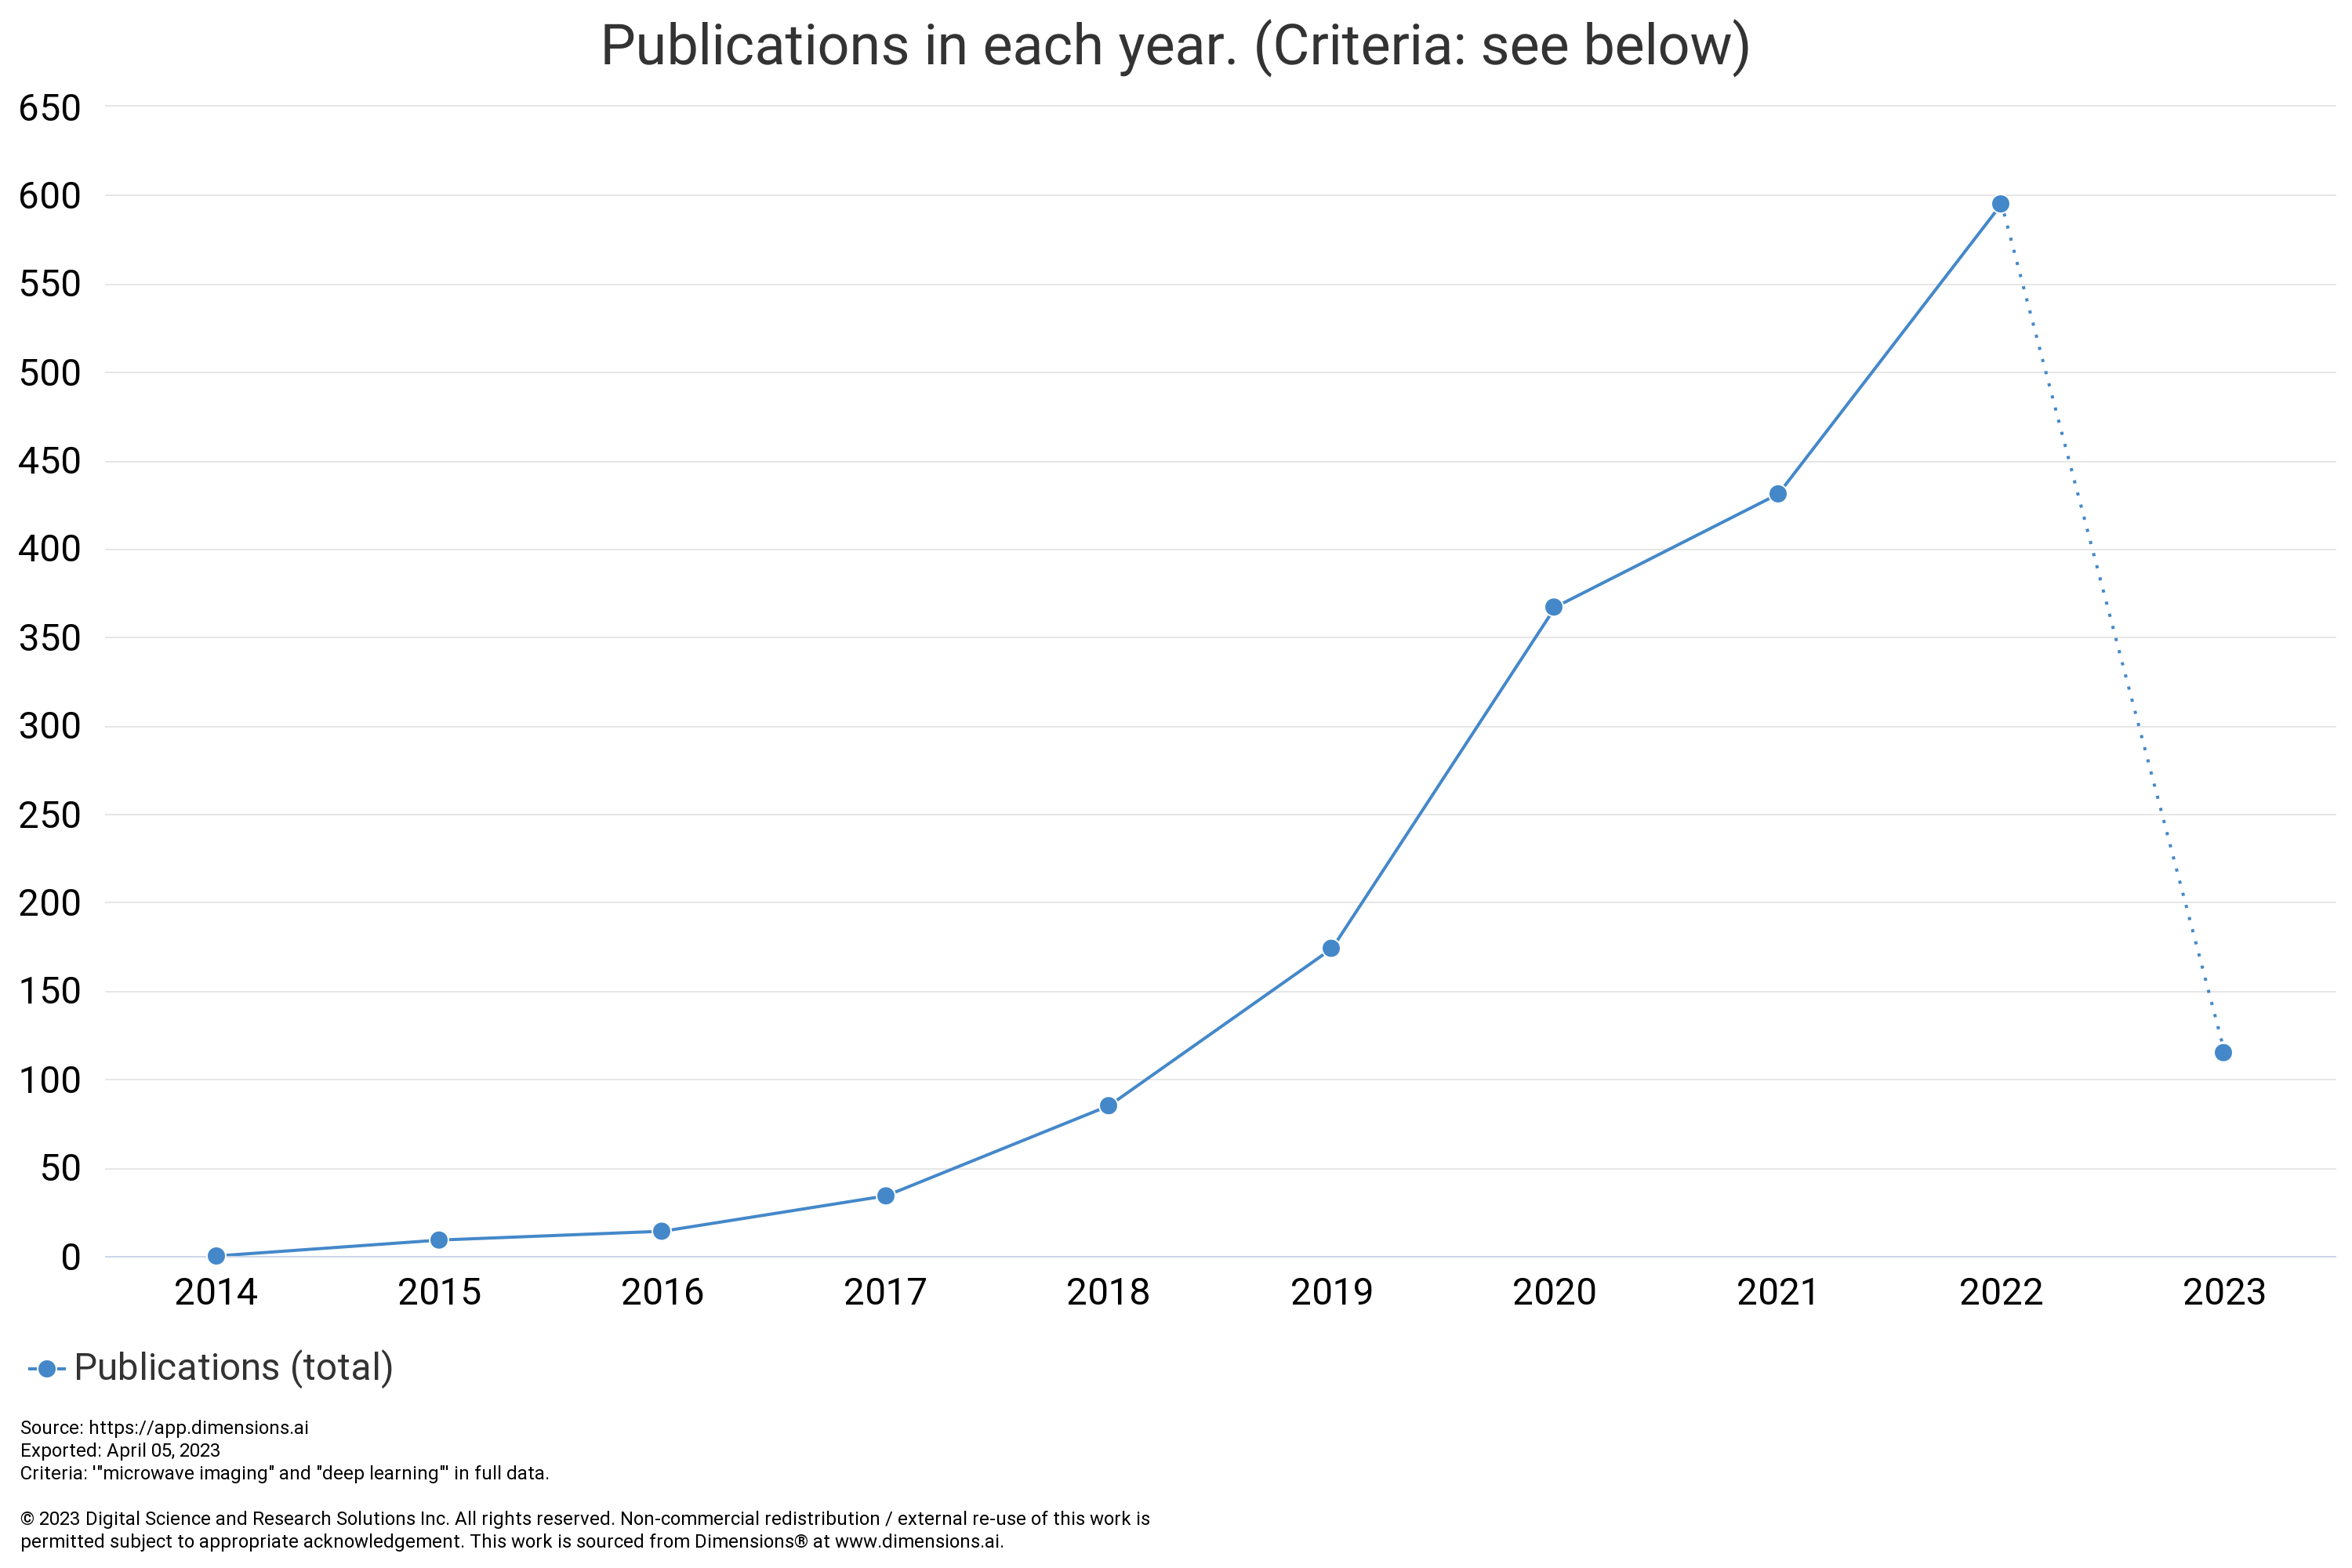
\includegraphics[width=\textwidth]{./figuras/chart.png}
			\caption[Emerging trends: the intersection of Microwave Imaging and Deep Neural Networks.]{Emerging trends: the intersection of Microwave Imaging and Deep Neural Networks garnering increasing attention among researchers, as reflected by the growth of published papers. Source: \url{http://app.dimensions.ai}}
			\label{fig:3:deeplearning}
		\end{figure}
		
		%Recentemente, \cite{chen2020review} fizeram uma revisão das metodologias DL aplicadas a EISP. De uma maneira geral, são destacadas três classes principais de métodos: Aprendizagem Direta (DL), Learning-Assisted Objective-Function (LAOF) e Physics-Assisted Learning (PAL). Para fazer a diferenciação entre as classes, os autores estabaleceram a divisão do problema inverso em três fases: (i) a propagação da onda incidente; (ii) a interação entre onda incidente e espalhador a qual induz corrente no espalhador; e (iii) a radiação da corrente induzida que propaga o campo espalhado. Interpretando essas fases à luz das equações de fonte de contraste \eqref{eq:2:eisp:5}-\eqref{eq:2:eisp:6}, somente a segunda fase depende da função contraste, i.e., na primeira e na terceira fases são preponderantes campo incidente e a fonte de corrente induzida, respectivamente.
		Recently, \cite{chen2020review} and \cite{salucci2022artificial} reviewed the DL methodologies applied to EISP. They highlighted three main classes of methods: Fully Data-Driven Learning, Learning-Assisted Objective-Function (LAOF), and Physics-Assisted Learning (PAL). The difference between them was established through the division of the scattering problem into three phases: (i) the propagation of the incident wave; (ii) the interaction between the incident wave and the scatterer which induces a current; and (iii) the radiation of the induced current that propagates the scattered field. Interpreting these phases in the light of the contrast source equations \eqref{eq:2:eisp:5}-\eqref{eq:2:eisp:6}, only the second phase depends on the contrast function, i.e., in the first and third phases, the incident field and the induced current source are predominant, respectively.
		
		%A classe DL é composta de métodos cuja a entrada da rede são os dados do campo espalhado e a saída é a função contraste, i.e., os métodos fazem um mapeamento direto da entre o campo espalhado e o contraste. Neste caso, é como se a rede fosse treinada para aprender as três fases do processo de espalhamento. Embora essa seja a implementação mais fácil, ela é pouco ineficiente tendo em vista que a rede é obrigada a aprender processo para os quais se têm uma forma analítica, como o caso da propagação do campo incidente. O custo computacional do treinamento é, portanto, muito alto, principalmente em casos da representação da solução por elementos lineares. Além disso, a performance pode ser muito ruim para múltiplos ou fortes espalhadores \citep{chen2020review}. Esse tipo de metodologia pode ser mais eficiente em casos mais simples onde já se tem informações sobre a formas dos espalhadores \citep{ran2019electromagnetic,fajardo2019phaseless}.
		The Fully Data-Drive Learning class is composed of methods whose input to the network is the scattered field data and the output is the contrast function, i.e., the methods make a direct mapping between scattered fields and contrast (Direct Learning Scheme). Therefore, the networks are trained to learn the three phases of the scattering process. Although this is the easiest implementation, it is not the most efficient one since the network is forced to learn processes for which they have an analytical form, such as the incident field propagation. The computational cost for the training phase is very high, especially when the solution is represented by linear elements. In addition, performance can be unsatisfactory for multiple or strong scatterers \citep{chen2020review}. This methodology can be efficient in simple cases where there is a priori information about the shapes of the scatterers \citep{ran2019electromagnetic,fajardo2019phaseless} or the media is assumed to be inhomogeneous \citep{zhang2023solving}. If a refinement network is added after the initial one, that is used to invert the scattered field data, it has the potential to further enhance the performance and achieve better results \citep{yao2019two,song2021electromagnetic,chen2022tailored}. Furthermore, there are additional techniques that can aid in enhancing the initial contrast estimation, such as inverting the Contract Integral Equation \eqref{eq:2:eisp:9} using Fourier bases \citep{xu2022learning} or adding acoustic data in the input \citep{qin2022breast}. Another approach involves predicting multi-frequency scattered fields based on a single-frequency one, which can alleviate the complexity of the direct inversion \citep{zhang2023enhanced}.
			
		%A Classe LAOF é baseada na utilização do aprendizado para acelerar a convergência de um método iterativo. Em outras palavras, pode ser inserido dentro dos métodos das seções \ref{chap:methods:deterministic} e \ref{chap:methods:stochastic} uma rede treinada para fornecer melhores direções de busca para acelerar a convergência. Um exemplo deste tipo de abordagem foi proposta em \citep{guo2019supervised}. Nela, os autores formularam um método de aprendizado de gradient, i.e., ao invés de calcular o gradiente para determinar a direção de minimização do erro, eles utilizam uma direção fornecida por uma rede treinada previamente para determinar a direção média de descida. Por isso, foi chamado de Método da Descida Supervisionada. Mas outros tipos de estratégias são possíveis: \cite{chen2020learning} proporam treinar uma rede para receber imagens de ressonância magnética e estimarem o contraste das imagens. Os resultados desse passo inicial foram acoplados no BIM para um refinamento da solução; similarmente, \cite{sanghvi2020embedding} proporam treinar uma rede para receber o vetor $\mathbf{\bar{J}^{eq}}_{s,+}$ da decomposição realizada pelo SOM e obter uma estimativa da fonte induzida total. Esta etapa combinada ao SOM contribui para a solução de problemas com espalhadores fortes.
		The LAOF Class is based on using deep-learning to accelerate the convergence of an iterative method. In other words, a trained network can be inserted into the methods of sections \ref{chap:methods:deterministic} and \ref{chap:methods:stochastic} to provide better search directions to accelerate convergence. An example of this type of approach was proposed in \citep{guo2019supervised}. The authors formulated a gradient learning method, i.e., instead of calculating the gradient to determine the direction of error minimization, they use one provided by a previously trained network to determine the average descent direction. For this reason, it was called the Supervised Descent Method. But other types of strategies are possible:
		\begin{enumerate}
			\item \cite{chen2020learning} proposed to train a network to receive magnetic resonance images and estimate the contrast of the images. The results of this initial step were coupled to the BIM to refine the solution;
			\item Similarly, \cite{sanghvi2020embedding} proposed to train a network to receive the $\mathbf{\bar{J}^{eq}}_{s,+}$ vector of the decomposition performed by SOM and obtain an estimate of the total induced source. This step combined with SOM contributes to the solution of problems with strong scatterers.
			\item \cite{yao2022enhanced} proposed a descent method where the forward problem in each iteration is solved by a complex-valued deep CNN.
		\end{enumerate}
			
		%O princípio da classe PAL é incorporar os aspectos físicos do problema dentro da formulação matemática da metodologia de aprendizado. Embora a alteração da estrutura interna da rede para adaptar as características peculiares do eletromagnetismo não seja uma tarefa trivial, Chen et al. também considera que esse príncipio pode ser utilizado na configuração da entrada da rede. Um exemplo disso é treinar a rede para que ela opere somente no espaço de soluções de contraste, i.e., um mapeador do espaço de soluções de contraste para ele mesmo. Na prática, isto significa treinar uma rede para que ela receba uma reconstrução inicial feita por algum método e retorne uma imagem de alta resolução e com contornos mais precisos do contraste verdadeiro. Em outras palavras, isto também significa predizer as componentes de alta frequência que estão faltando a partir de uma imagem com componentes de baixa frequência. Exemplos deste tipo de abordagem que ser encontrados na literatura são: (i) diferentes estruturas de redes desenvolvidas para receber a imagem reconstruída pela método Back-Propagation \citep{sun2018efficient,wei2019deep,li2019deepnis,li2019performance}; (ii) a estimativa do contraste pela Aproximação de Born, seguida de um refinamento feito pelo Método Monte Carlo e posterior refinamento feito por uma NN \citep{xiao2020fast}; e (iii) a rede treinada a partir de reconstruções feitas pelo CSI \citep{khoshdel2019enhancement}. Como exemplo de adaptação da estrutura interna de uma NN para incorporar os aspectos físicos do problema e fazer um mapeamento entre campo espalhado e contraste, podemos citar o artigo escrito por \cite{khoo2019switchnet}. Neste trabalho, os autores propõem uma camada de conexões esparsas a qual leva em consideração a Aproximação de Born e o padrão de campo distante. Os autores também destacam a importância que as conexões esparsas têm para reduzir o custo do treinamento por reduzir o número de parâmetros. Além disso, afirmam que a aplicação de Redes Neurais Convolucionais (CNN) neste caso é inviável pois sua estrutura não é compatível característica global do impacto do espalhador sobre o campo espalhado.
		The PAL class principle is to incorporate the physical aspects of the problem into the mathematical formulation of the network architecture. Although adapting the internal structure to combine the electromagnetism laws is not a trivial task, \cite{chen2020review} also consider that this principle can be used in the configuration of the network input. An example is to train the network to operate only in the space of contrast solutions, i.e., a mapper of the contrast solutions space for itself. In practice, this means training a network to receive an initial reconstruction done by some method and return a high-resolution image with more precise contours of the true contrast. In other words, this also means predicting the high-spatial-frequency components that are missing from an image with the low ones. Examples of this approach in the literature are:
		\begin{enumerate}
			\item Different network structures developed to receive the image reconstructed by linear methods such as Born Approximation, Back-Propagation, and Dominant Current \citep{sun2018efficient,wei2019deep,li2019performance,xiao2020fast,guo2021complex,zong2022wavelet}. Specifically, \cite{wei2022exploring} suggested using each contrast image obtained by each incident angle in the Back-Propagation method as the input of the network.
			\item The refinement of images recovered Near-Field Scanning Microwave Microscopy \citep{zhou2023physics};
			\item The network trained from reconstructions made by the CSI \citep{khoshdel2019enhancement};
			\item The threefold hybrid method that recovers the shape through LSM, refine it through CNN, and estimate the dielectric properties by BIM \citep{chen2021quantitative};
			\item \citep{zhang2020learning} proposed the combination of a qualitative and quantitative approach as an input to a CNN.
			\item In \citep{chen2020learning}, the authors proposed an approach that utilized Convolutional Neural Networks (CNN) to estimate dielectric properties from Magnetic Resonance images. This estimated property was then used as an initial guess for a qualitative inversion method.
		\end{enumerate}
		
		In an effort to integrate physical principles into neural network structures, researchers have utilized the iterative nature of quantitative inversion methods. This approach is also known as unrolled method and has been investigated in the most recent research papers. They has consistently demonstrated improved network performance. Notable examples of such papers include:
		\begin{enumerate}
			% \item \cite{khoo2019switchnet} proposed a layer of sparse connections which takes into account the Born Approximation and the distant field pattern. The authors also highlight the importance that sparse connections have to reduce the training cost by reducing the number of parameters. In addition, they claim that the application of Convolutional Neural Networks (CNN) in this case is impracticable because its structure is not compatible with the global nature of the impact of the scatterer on the scattered field.
			\item \cite{li2019deepnis} proposed a cascade of CNN stages that represents the recursive solution derived from the regularization of the inverse problem.
			\item \cite{liu2022physical} introduced a comparable architecture, but with a distinct feature. In this structure, each stage consists of four layers dedicated to predicting four different variables: induced current, total field, contrast image, and an auxiliary variable.
			\item In the method proposed by \cite{liu2022somnet}, the induced current and contrast map from the previous stage are combined to generate a novel prediction of the induced current. This approach was compared to SOM.
			\item \cite{shan2023neural} put forward a novel approach to enhance BIM framework by utilizing two CNNs in place of the conventional forward and inverse solvers. Consequently, each stage of the updated framework was characterized as an iteration of BIM.
			\item \cite{zhang2023unrolled} has proposed a novel approach in which each stage comprises of two Contrast Source Inversion (CSI) iterations and two Convolutional Neural Networks (CNNs). In the first CSI iteration, the contrast image is updated, following which the two CNNs predict the residual between the correct image and the present one. This information is then fed into another CSI iteration that fine-tunes the current contrast image for further improvement.
			\item \cite{zhou2022deep} has presented a Generative Adversarial Network (GAN) where each stage of the generative network implements an iteration of CSI in which each variable is a layer, similarly to \cite{liu2022physical}. In addition, they incorporated a refinement layer after predicting the contrast image to further enhance the reconstruction.
		\end{enumerate}
		
		
		% Alternatively, the internal structure of a NN might be adapted to incorporate the physical aspects of the problem and mapping between scattered fields and contrast.
		%As an example of adapting the internal structure of a NN to incorporate the physical aspects of the problem and mapping between scattered fields and contrast, we can cite the article written by \cite{khoo2019switchnet}. In this work, the authors propose a layer of sparse connections which takes into account the Born Approximation and the distant field pattern. The authors also highlight the importance that sparse connections have to reduce the training cost by reducing the number of parameters. In addition, they claim that the application of Convolutional Neural Networks (CNN) in this case is impracticable because its structure is not compatible with the global nature of the impact of the scatterer on the scattered field.
		
		%Embora questões sobre o tamanho do conjunto de treinamento e a capacidade de generalização representem dúvidas sobre o limites de aplicação, o esforço para progresso do desenvolvimento de DLs para EISPs é notório na literatura. E o sentido de desenvolvimento defendido por \cite{chen2020review} é busca por adaptações nas arquiteturas gerais de NN para que sua operações cada vez mais levem em consideração as aspectos físicos do problema. Em outras palavras, que a física faça esteja menos no aprendizado das NNs e mais na própria estrutura. Isso é equivalente a encurtar a distância que existe entre as técnicas produzidas pelo desenvolvimento dos métodos determinísticos com as de aprendizado de máquina.
		%Although issues about the size of the training set and the ability to generalize represent challenges concerning the application limits, the effort to develop DLs for EISPs is notorious in the literature. And, as asserted by \cite{chen2020review}, the opportunities are in the research for adaptations in the general NN architectures and operations to increasingly take into account the physical aspects. In other words, physics should be embedded into the structure rather than being what is learned. This is equivalent to shortening the distance that exists between the techniques developed for deterministic methods with those of machine learning.
		
		%Uma estrutura promissora de NNs é a Generative Adversarial Network (GAN) comumente aplicada para traduções de imagens \citep{goodfellow2014generative}. Esta técnica é baseada na ideia de competição entre duas redes. A rede que é treinada para fazer o mapeamento também gera novas instâncias e pra que os resultados sejam comparados em uma segunda rede cujo o objetivo é conseguir distinguir entre o que é o resultado verdadeiro do que é o falso. Deste modo, quanto maior o erro desta segunda rede, mais qualificada a primeira é. Recentemente, \cite{ma2021learning} proporam uma abordagem utilizando uma variante do GAN para predizer a fonte de corrente induzida num problema direto. Este trabalho está inserido dentro de um projeto de primeiro entender como os conceitos físicos podem moldar a estrutura de uma NN para um problema direto e, a partir daí, traduzir os conceitos para o problema inverso. Outros dois trabalhos relevantes publicados após o artigo de revisão mencionado anteriormente são: (i) a combinação de uma abordagem qualitativa e quantitativa como entrada de uma CNN \citep{zhang2020learning}; e (ii) uma reformulação do FFT-SOM utilizando a integral \eqref{eq:2:eisp:9} e acoplado numa CNN, considerando os casos bi- e tridimensionais \citep{zhou2021improved}.
		%A promising structure is the Generative Adversarial Network (GAN), commonly applied for image translations \citep{goodfellow2014generative}. This technique is based on the idea of competition between two networks. The network that is trained to do the mapping also generates new instances in which their results are compared in a second network whose objective is distinguishing between what is the true result and what is the predicted one. Thus, the greater the error of the second network, the more qualified the first is.
		%Recently,\cite{ma2021learning} proposed an approach using a variant of GAN to predict the induced current source in a forward problem. This work is part of a project in which the first goal is to understand how physical concepts can shape the structure of a NN to a direct problem and, from there, translate these concepts to the inverse problem. Two other relevant works published after the mentioned review are: (i)  and (ii) a reformulation of the FFT-SOM using the integral \eqref{eq:2:eisp:9} and coupled to a CNN, considering two and three-dimensional cases \citep{}.
				
		DL techniques have found applications beyond the inverse two-dimensional problem. Researchers have explored the use of these techniques for solving three-dimensional problems \citep{chen2023mesh,han2022hybrid,khoshdel2021multi,zhou2021improved,xiao2022hybrid,zhao2022machine} and for estimating fields in the forward problem \citep{guo2022physics,ma2021learning,seretis2022toward,yao2023implementing,yin2022electric,hu2022theory}. Additionally, peripheral issues have been addressed in the literature: learning regularization parameters \citep{afkham2021learning}; independence of measurement configuration \citep{li2023transceiver}; phase information \citep{pan2021phase} and prediction \citep{luo2022cascaded}; scatterer and background classification for qualitative methods \citep{ruiz2022physics}; dielectric breast phantoms generated by GAN \citep{shao2022dielectric}; and the inversion of dielectric and perfect electric conductor scatterers \citep{song2022learning}.

	\section{Conclusion}\label{chap:methods:conclusion}
		
		%Este capítulo apresentou uma revisão sobre as metodologias de solução de EISP. Com objetivo de facilitar a tradução das ideias em implementação numérica, foi feito um esforço na definição da discretização do problema na Seção \ref{chap:methods:discretization} baseado em um esquema comum do problema definido na Seção \ref{chap:methods:definition}. Destaca-se a discretização de \eqref{eq:3:discretization:collocation:3}-\eqref{eq:3:discretization:collocation:7} a qual é a forma mais popular na literatura, bem como a forma matricial em \eqref{eq:3:discretization:collocation:10}-\eqref{eq:3:discretization:collocation:14}. Em, foram apresentadas as abordagens lineares como a Aproximação de Born e a de Rytov (Subseção \ref{chap:methods:linear:weak}) bem como as metodologias clássicas de regularização de problemas inversos lineares mal-postos, como a Regularização de Tikhonov (Subseção \ref{chap:methods:linear:tikhonov}) com seus vários métodos de escolha sendo a Curva-L um dos principais (Subsubseção \ref{chap:methods:linear:tikhonov:lcurve}).
		This chapter has reviewed the EISP solution methodologies. To facilitate the translation of ideas into numerical implementation, an effort was made to define the problem discretization in Section \ref{chap:methods:discretization} based on a usual problem configuration defined in \ref{chap:methods:definition}. We highlight the discretization of \eqref{eq:3:discretization:collocation:3}-\eqref{eq:3:discretization:collocation:7} which is the most popular form in the literature, as well as the matrix form in \eqref{eq:3:discretization:collocation:10}-\eqref{eq:3:discretization:collocation:14}. Then, linear approaches such as the Born and Rytov approximations and the Back-Propagation and Dominant Current methods were presented. The classic regularization methodologies, often required for solving linear ill-posed inverse problems, were also presented. We mention the Tikhonov Regularization (Subsection \ref{chap:methods:linear:tikhonov}) with its several parameter choice methods, where the L-Curve is one of the main ones (Subsection  \ref{chap:methods:linear:tikhonov:lcurve}).
		
		%Os métodos não-lineares são classificados ou como determinísticos (Seção \ref{chap:methods:deterministic}) ou como estocásticos (Seção \ref{chap:methods:stochastic}). A principal vantagem dos determinísticos é a reconstrução a partir de informações concretas sobre o problema físico, enquanto que a vantagem dos algoritmos estocásticos é a sua compatibilidade com problemas não-lineares e com múltiplos mínimos. Entre o determinísticos, os mais tradicionais são BIM (Subseção \ref{chap:methods:deterministic:bim}), DBIM (Subseção \ref{chap:methods:deterministic:dbim}) e o CSI (Subseção \ref{chap:methods:deterministic:csi}), enquanto os que tem mais sido mais utilizados nos trabalhos recentes são o CS (Subseção \ref{chap:methods:deterministic:cs}), Level-Set (Subseção \ref{chap:methods:deterministic:levelset}) e SOM (Subseção \ref{chap:methods:deterministic:som}). Consideramos os estocásticos, destacamos os algoritmos evolutivos que podem ser adaptados para diversos tipos de representações (Subseção \ref{chap:methods:stochastic:representation}), funções-objetivo (Subseção \ref{chap:methods:stochastic:objfun}), mecanismos e operações de busca (Subseção \ref{chap:methods:stochastic:mechanism}); e inicializações (Subseção \ref{chap:methods:stochastic:initialization}). As formulações mais atuais normalmente consideram uma representação da solução pelos elementos de discretização, o mecanismo do PSO, a ponderação dos resíduos das equações de dados e estados. Uma das estratégias mais bem sucedidas de redução do problema é a IMSA.
		Nonlinear methods are classified as either qualitative or quantitative. The former is suitable for when only the shape of the scatterers are necessary to recover. On the other hand, the latter is the class for when shape and dielectric information need to be estimated. The quantitative methods are divided into deterministic (Section \ref{chap:methods:deterministic}) or stochastic (Section \ref{chap:methods:stochastic}) methods. The main advantage of deterministic methods is the reconstruction by operations that are fully based on the physical properties while the advantage of stochastic algorithms is their compatibility with nonlinear problems with multiple minimums. Among the deterministic ones, the most traditional ones are BIM (Subsection \ref{chap:methods:deterministic:bim}), DBIM (Subsection \ref{chap:methods:deterministic:dbim}), and CSI (Subsection \ref{chap:methods:deterministic:csi}) while the ones that have been most used in recent works are CS (Subsection \ref{chap:methods:deterministic:cs}), Level-Set (Subsection \ref{chap:methods:deterministic:levelset}) and SOM (Subsection \ref{chap:methods:deterministic:som}). Considering the stochastic methods, we highlight the evolutionary algorithms that can be adapted for different types of representations (Subsection \ref{chap:methods:stochastic:representation}), objective functions (Subsection \ref{chap:methods:stochastic:objfun}), search engines and operations (Subsection \ref{chap:methods:stochastic:mechanism}); and initializations (Subsection \ref{chap:methods:stochastic:initialization}). The latest formulations usually consider a representation of the solution by the discretization elements, the PSO mechanism, the weighted residuals of data and state equations. One of the most successful strategies to reduce the problem is IMSA and the replacement of the objective function by surrogate models. Table \ref{tab:methods:conclusion} summarizes the various methods according to their properties.
		
		%Por fim, foi feita uma breve discussão sobre a utilização de DLs (Seção \ref{chap:methods:deep}), normalmente acoplados a estratégias determinísticas lineares ou não, para o refinamento e maior resolução da função contraste. Esse assunto tem recebido muita atenção da literatura atualmente representando uma principais direções de pesquisa e desenvolvimento de metodologias para o problema.
		Finally, a brief discussion was made on the use of DLs (Section \ref{chap:methods:deep}), usually coupled with linear or non-linear deterministic strategies for the refinement and resolution increase of the contrast image. This subject has received a lot of attention from the literature recently and it represents one of the main research opportunities for the development of methodologies that address EISP.
		
		\begin{table}[]
			\setstretch{1.5}
			\caption{Classification of methods by their properties.}
			\label{tab:methods:conclusion}
			\begin{tabular}{clm{2cm}m{2cm}m{6cm}}
				\hline
				Classes & \multicolumn{4}{c}{Methods} \\ \hline
				\multirow{2}{*}{Qualitative} & \multicolumn{4}{l}{Linear Sampling Method} \\
				& \multicolumn{4}{l}{Orthogonality Sampling Method} \\ \hline
				\multirow{26}{*}{Quantitative} & \multirow{15}{*}{Deterministic} & \multirow{4}{*}{Linear} & \multicolumn{2}{l}{Born Approximation} \\
				&  &  & \multicolumn{2}{l}{Rytov Approximation} \\
				&  &  & \multicolumn{2}{l}{Back-Propagation Method} \\
				&  &  & \multicolumn{2}{l}{Dominant Current Scheme} \\ \cline{3-5} 
				&  & \multirow{11}{*}{Nonlinear} & \multirow{4}{*}{\makecell[l]{Forward\\and\\inverse\\subproblems}} & Born Iterative Method \\
				&  &  &  & Distorted Born Iterative Method \\
				&  &  &  & Variational Born Iterative Method \\
				&  &  &  & Level-Set Method \\ \cline{4-5} 
				&  &  & \multirow{3}{*}{\makecell[l]{Gradient-\\based}} & Conjugated-Gradient Method \\
				&  &  &  & Contrast Source Inversion \\
				&  &  &  & Subspace-based Optimization Method \\ \cline{4-5} 
				&  &  & \multirow{4}{*}{Other} & Compressive Sensing \\
				&  &  &  & Regularization on Lp Banach Spaces \\
				&  &  &  & Virtual Experiments \\
				&  &  &  & Deep learning methods \\ \cline{2-5} 
				& \multirow{11}{*}{Stochatisc} & Components & \multicolumn{2}{l}{Types} \\ \cline{3-5} 
				&  & \multirow{3}{*}{\makecell[l]{Representa-\\tion}} & \multicolumn{2}{l}{Known geometries} \\
				&  &  & \multicolumn{2}{l}{Contours} \\
				&  &  & \multicolumn{2}{l}{Pixel-based} \\ \cline{3-5} 
				&  & \multirow{2}{*}{\makecell[l]{Objective\\function}} & \multicolumn{2}{l}{Data equation residual} \\
				&  &  & \multicolumn{2}{l}{Data and state equation residual} \\ \cline{3-5} 
				&  & \multirow{3}{*}{Mechanism} & \multicolumn{2}{l}{GA} \\
				&  &  & \multicolumn{2}{l}{DE} \\
				&  &  & \multicolumn{2}{l}{PSO} \\ \cline{3-5} 
				&  & \multirow{2}{*}{\makecell[l]{Population\\Initialization}} & \multicolumn{2}{l}{Random} \\
				&  &  & \multicolumn{2}{l}{Born Approximation} \\\hline
			\end{tabular}
		\end{table}
		

%% COISAS QUE VAO FICAR PRA DEPOIS
% 1) Escolha do parâmetro do regularizador de Tikhonov por periogram: Mojabi, Puyan, and Joe LoVetri. "Preliminary Investigation of the NCP Parameter-Choice Method for Inverse Scattering Problems Using BIM: 2-D TM Case." ACES. 2008.
% 2) Resolver o problema no espaço de Banach ao invés de Hilbert. Desse artigo pra frente: C. Estatico, M. Pastorino and A. Randazzo, "A Novel Microwave Imaging Approach Based on Regularization in $L^{p}$ Banach Spaces," in IEEE Transactions on Antennas and Propagation, vol. 60, no. 7, pp. 3373-3381, July 2012, doi: 10.1109/TAP.2012.2196925.
% 3) Back-propagation. Achar as equações em: Sun, Yu, Zhihao Xia, and Ulugbek S. Kamilov. "Efficient and accurate inversion of multiple scattering with deep learning." Optics express 26.11 (2018): 14678-14688.
% 4) Eu acho que poderia vir aqui uma discussão sobre a medição dos resultados, de qualidade da imagem. Ou uma discussão sobre experimentação. Tanto pra eu mostrar que a maioria dos trabalhos usam o erro percentual médio como avaliador de qualidade da imagem como citar os dados reais do Instituto de Fresnel e das mamas da Hagness.

    % ------------------------------------------------------------------------------
% Proposed Methodology
% ------------------------------------------------------------------------------

\chapter{Proposed Methodology}\label{chap:proposed-methodology}

	This thesis aims to enhance the current state-of-the-art algorithms for microwave imaging by proposing novel approaches based on surrogate models. Additionally, a comprehensive framework for the development and testing of algorithms specific to this problem is presented. In Section \ref{chap:proposed-methodology:criticism}, a critical review of the literature is presented, highlighting the gaps and areas for improvement in the current state of the art. Building on this analysis, Section \ref{chap:proposed-methodology:proposal} proposes a novel approach to address some of the limitations, specifically, the use of surrogate models and the framework for development and comparison of algorithms designed for EISPs. Section \ref{chap:proposed-methodology:surrogate} provides a detailed discussion of surrogate-model assisted algorithms for microwave imaging, including a description of the transformation of the inversion problem into a bidimensional optimization one, the Kriging model, and the proposed algorithms. Section \ref{chap:proposed-methodology:library} outlines a framework for developing and testing algorithms for microwave imaging, including the proposed metrics to assess their performance. Finally, Section \ref{chap:proposed-methodology:conclusion} presents the concluding remarks.

	\section{Literature Criticism and Opportunities}\label{chap:proposed-methodology:criticism}
	
		In the early stages of developing algorithms for microwave imaging, several challenges were encountered \citep{kirsch2011introduction,pastorino2000microwave,bertero2020introduction}. In the early context, the available data was significantly limited and noisy, which represented a serious challenge for a problem with non-unique solution. When more data was available, the limited computing power was other challenge. The understanding of the physics involved in microwave imaging also evolved throughout the years, which was also important for the development of the subject.
	
		Currently, two significant challenges are faced by researchers in the literature: real-time imaging and the retrievement of strong scatterers. Real-time imaging requires fast and efficient algorithms that can produce accurate images in real-time or nearly, which is essential for many applications such as medical imaging \citep{li2021machine} and security screening \citep{asok2022concealed}. To address this challenge, researchers have turned to deep-learning techniques that can efficiently process large amounts of data and provide accurate results in real-time \citep{salucci2022artificial}.
		
		The other challenge is the imaging of strong scatterers, which refers to objects with high contrast levels or large dimensions when comparing to the wavelength. Such objects result in high nonlinearity and can create significant artifacts in the resulting image, making it difficult to accurately reconstruct the underlying structure. This is particularly challenging when imaging complex structures, such as biological tissues or composite materials \citep{lazebnik2007large}. This type of scenario has been addressed in three main ways:
		\begin{enumerate}
			\item The first approach is to reduce the degree of non-linearity by changing the integrals solved by the algorithms (Section \ref{chap:problemstatement:eisp});
			\item The second approach is based on domain decomposition \citep{zhang2022iterative}. This approach divides the scatterer region into dominant and subordinate subdomains based on the information of the induced current. The dominant subdomain is then reconstructed iteratively, narrowing the inversion domain and reducing the nonlinearity of the problem.
			\item The third approach is the use of surrogate models \citep{koziel2008engineering}. \cite{salucci2022learned} proposed a surrogate model to predict the data equation error considering curve-based representations of scatterers. By using this approach, the computational cost of stochastic algorithms that do not solve the contrast and the total field simultaneously can be significantly reduced. This is because such algorithms rely on forward problem simulations to estimate the error. The authors demonstrated the effectiveness of their approach in high-contrast scenarios, showing promising results.
		\end{enumerate}
		
		Some ideas in the field have yet to receive the attention they deserve, and one of them is the use of qualitative methods to define initial solutions for quantitative algorithms. Even though this approach has been explored in some papers \citep{zhang2020learning,han2022hybrid,bevacqua2015algebraic}, it has yet to be fully utilized to improve the performance of stochastic algorithms for the problem. The use of qualitative methods can help to improve the robustness of images reconstructed by these algorithms to noise and high contrasts, as well as guide the convergence of population-based algorithms towards more promising regions of the search space.
		
		%Outro aspecto que chama a atenção na literatura é o design dos experimentos e a avaliação da qualidade dos algoritmos. É necessário destacar que um aspecto extremamente relevante para a experimentação é a utilização de modelos de espalhadores mais realísticos ou dados obtidos de medições reais. Isto tem ficado popular na literatura através laboratórios que disponibilização os dados. Dois exemplos muito comuns são o \textit{UWCEM Numerical Breast Phantom Repository} \citep{burfeindt2012mri} e as medições realizadas pelo \textit{Institut Fresnel} \citep{geffrin2005free}. 
		Another aspect that draws attention in the literature is experiment design and quality evaluation of algorithms. A highly relevant aspect of experimentation is using more realistic scatterer models or data obtained from real measurements. This has become popular in the literature through laboratories that make the data available. Two widespread examples are the \textit{UWCEM Numerical Breast Phantom Repository} \citep{burfeindt2012mri}  and the measurements made by the \textit{Institut Fresnel} \citep{geffrin2005free}.
		
		In addition, \cite{kurrant2021evaluating} have recently proposed a methodology to evaluate the performance of the algorithms applied to breast cancer detection. Given a reference image and the recovered one, the authors proposed to segment the tissues in the images by an unsupervised machine learning approach. After decomposing the images and mapping the tissues, five metrics were proposed to evaluate shape fidelity, malignant tissue reconstruction in tumor regions, among others. Therefore, the novelty is a technique to measure the quality of breast reconstruction with suitable tools. Their methodology is also available as a MATLAB toolbox \citep{kurrant2021mwsegeval}.
		
		%No entanto, os autores das publicações tradicionalmente escolhem instâncias com características particulares com o objetivo de demonstrar a capacidade de reconstrução do método proposto na correspondente situação. A partir disso, a performance é medida através de algum indicador de qualidade e o resultado é comparado a outros algoritmos e formulações \citep{zhong2020multiresolution,zhang2020wavelet,zhou2021improved}. Embora essa abordagem seja interessante para ilustrar a capacidade do algoritmo, ela tem pouco rigor metodológico para oferecer respostas robustas à perguntas como: (i) qual impacto da escolha da instância no valor do quantificador da performance? (ii) Como o indicador varia se a geometria do objeto mudar? (iii) Como a diferença na performance observada entre os dois métodos varia se as geometrias variarem? (iv) Qual a performance média ou pior caso do método para uma dada configuração? (v) Etc.
		However, in many publications addressing general applications, traditional instances have been chosen with particular characteristics to demonstrate the reconstruction ability of the proposed method in the corresponding situation. Performance is measured through some quality indicator, and the result is compared to other algorithms and formulations \citep{zhong2020multiresolution,zhang2020wavelet,zhou2021improved}. Although this approach is interesting to illustrate the algorithm's suitableness, it has little methodological rigor to offer robust answers to questions such as: (i) what is the impact of the choice of the instance on the performance quantifier's value? (ii) How does the indicator vary if the object's geometry changes? (iii) How does the difference in performance observed between the two methods vary if the geometries vary? (iv) What is the average or worst-case performance of the method for a given configuration? Among others.
		
		%Mesmo que essas perguntas possam fugir do escopo de propostas baseadas em um estudos de caso (e.g., experimentos reais), conclusões gerais sobre a capacidade e performance podem ser muito fracas sem uma metodologia experimental adequada que leve em consideração diferentes fatores de efeito na configuração do problema. Embora o fator de nível de ruído costume ser o mais explorado nesse sentido \citep{chew1990reconstruction,chen2010subspace,shah2018fast,batista2021quadratic}, uma experimentação com instâncias aleatórias para uma medição mais robusta da performance não foi levada em consideração nem quando a publicação tinha como objetivo principal a comparação entre algoritmos \citep{moghaddam1991comparison,gilmore2009comparison,pan2010comparison}. Este tipo de prática é essencial para eliminar o viés do observador em análises de algoritmos \citep{montgomery2010applied}. Um outro exemplo sobre isso é a existência de vários trabalhos na literatura que propõem metodologias estocásticas e nem ao menos informam quantas vezes o algoritmo foi repetido quando exibem o resultado para uma dada instância. Não há informação se o resultado mostrado representa o pior, médio ou melhor caso, como se fosse o resultado único de um tipo de metodologia que não tem garantia nenhuma de retornar a mesma solução em toda execução \citep{massa2005parallel,ashtari2010using,salucci2017multifrequency}.
		Even though these questions may fall outside the scope of proposals based on case studies (e.g., physical experiments), general conclusions about suitability and performance can be very weak without an adequate experimental methodology that considers different effect factors in the configuration of the problem. Although the noise level factor is usually the most explored in this sense \citep{chew1990reconstruction,chen2010subspace,shah2018fast,batista2021quadratic}, experiments with random instances for a more robust measurement performance are not usually performed. Even when the publication had the main objective of comparing algorithms \citep{moghaddam1991comparison,gilmore2009comparison,pan2010comparison}. This practice is essential to eliminate the observer's bias in algorithms analysis \citep{montgomery2010applied}. Other examples are several works in the literature that propose stochastic methodologies and do not even inform how many times the algorithm was repeated when showing the result for a given instance. There is no information if the result shown represents the worst, average, or best case. This is problematic since these methodologies have no guarantee of returning the same solution in every execution \citep{massa2005parallel,ashtari2010using,salucci2017multifrequency}.
		
		%Por isso, uma oportunidade na literatura é introduzir comparações mais robustas entre algoritmos. Uma referência sobre boas práticas de comparação de algoritmos de otimização é o artigo escrito por \cite{beiranvand2017best}. Entre muitos apontamentos relevantes feitos pelos os autores, destacamos os seguintes:
		Therefore, another opportunity in the literature is to introduce more robust comparisons between algorithms, i.e., benchmarking. A reference on best practices for comparing optimization algorithms is the article written by \cite{beiranvand2017best}. Among the many relevant notes made by the authors, we highlight the following:
		
		\begin{itemize}
			%\item Um conjunto de teste com poucos problemas deve ser referido como um estudo de caso ou prova de conceito, mas não benchmarking.
			%\item Um conjunto de teste deve evitar as seguintes deficiências: (i) poucos problemas; (ii) pouca ou excessiva variação na complexidade das instâncias inviabilizando a extração de informações úteis; (iii) problemas sem soluções conhecidas (o qual pode ser inevitável em situações reais); (iv) viés no ponto de partida dos algoritmos; (v) estruturas escondidas (e.g., arredondamento de números). 
			%\item Todos algoritmos devem receber a mesma quantidade de informação de entrada e garantir que não há um pressuposto que é respeitado somente por um dos algoritmos.
			\item A test suite with few problems should be referred to as a case study or proof of concept, but not benchmarking.
			\item A test suite should avoid the following deficiencies: (i) few problems; (ii) slight or excessive variation in the complexity of the instances, making it impossible to extract helpful information; (iii) problems with no known solutions (which can be inevitable in real situations); (iv) bias at the starting point of the algorithms; (v) hidden structures.
			\item All algorithms must receive the same amount of input information and ensure that there is an assumption that is only respected by one of the algorithms in order to verify the influence of that assumption.
		\end{itemize}
		
		%Esses tópicos não representam necessariamente falhas nas experimentações descritas na literatura. No entanto, esses conceitos já estabelecidos na literatura sobre otimização podem trazer amadurecimento na de algoritmos para EISP.
		These topics do not necessarily represent failures in the experiments described in the literature. However, these concepts already established in the optimization literature can bring maturity to the algorithms for EISP.
		
		%Por fim, destacamos também as métricas utilizadas para avaliar a qualidade das reconstruções. Na vasta maioria dos trabalhos, a qualidade das imagens reconstruídas da função contraste é quantificada por uma das seguintes formas \citep{wang1989iterative,chew1990reconstruction,shah20193d,oliveri2019compressive,oliveri2011multiresolution,salucci2017multifrequency,zhang2020learning}:
		Finally, we also highlight the metrics used to assess the quality of the reconstructions. In the vast majority of works, the quality of the reconstructed images of the contrast function is quantified in one of the following ways \citep{wang1989iterative,chew1990reconstruction,shah20193d,oliveri2019compressive,oliveri2011multiresolution,salucci2017multifrequency,zhang2020learning}:
		\begin{align}
			\zeta_{\epsilon} &= \sqrt{\frac{1}{N_IN_J}\sum\limits_{i=1}^{I}\sum\limits_{j=1}^J\left|\frac{\epsilon^*_{r,ij}-\epsilon_{r,ij}}{\epsilon^*_{r,ij}}\right|^2} \label{eq:4:error0:epsilon} \\
			\zeta_{\chi} &= \sqrt{\frac{1}{N_IN_J}\sum\limits_{i=1}^{I}\sum\limits_{j=1}^J\left|\frac{\chi^*_{ij}-\chi_{ij}}{\chi^*_{ij}+1}\right|^2} \label{eq:4:error0:chi}
		\end{align}
		
		%\noindent onde $\epsilon^*_{r,ij}$ e $\chi^*_{ij}$ são os valores verdadeiros de permissividade relativa e contraste, respectivamente. Ou seja, de um modo geral, \eqref{eq:4:error0:epsilon} e \eqref{eq:4:error0:chi} são fórmulas baseadas na raiz da média do erro percentual. Pequenas variações nelas também podem ser adotadas, como a substituição de $N_IN_J$ pela área da imagem ou pela remoção da raiz e do quadrado do erro.
		\noindent where $\epsilon^*_{r,ij}$ and $\chi^*_{ij}$ are the actual values of relative permittivity and contrast, respectively. In general, \eqref{eq:4:error0:epsilon} and \eqref{eq:4:error0:chi} are formulas based on the root of the average percentage error. Slight variations can also be adopted, such as replacing $N_IN_J$ with the image area or removing the root and square of the error.
		
		%De um modo geral, quando se trata de identificar objetos na imagem, uma boa reconstrução é caracterizada pela identificação correta da posição, da forma e do contraste do espalhador. \eqref{eq:4:error0:epsilon} e \eqref{eq:4:error0:chi} são métricas que abordam essas três características ao mesmo. Uma reconstrução igual à verdadeira vai minimizar esses indicadores. No entanto, existem situações nas quais esses indicadores não são tão eficientes. Quando a área de um espalhador é muito menor que a da figura, o erro vai ser bem pequeno mesmo que haja muitos desvios na estimativa do contraste na área do espalhador (e.g., $\chi=0$). Isto pode também disfarçar erros significativos na posição e forma dos espalhadores reconstruídos. Vale à pena notar que os resíduos das equações não são tomados necessariamente como medidores de qualidade tendo em vista que, por causa da má-posição do problema, podem haver soluções com baixo resíduos e imagens diferentes das esperadas.
		In general, when it comes to identifying objects in the image, a good reconstruction is characterized by the correct identification of the scatterer's position, shape, and contrast. \eqref{eq:4:error0:epsilon} and \eqref{eq:4:error0:chi} are metrics that address these three characteristics at the same time. A reconstruction equal to the actual one will minimize these indicators. However, there are situations in which these indicators are not as efficient. When the area of a scatterer is much smaller than the figure, the error will be minimal. This might happen even if there are many deviations in the estimate of the contrast in the scatterer area (e.g., $\chi=0$). This can also disguise significant errors in the position and shape of the rebuilt scatterers. It is worth noting that the residuals of the equations are not necessarily taken as quality meters, given that, due to ill-posedness, there may be solutions with low residues and images that are different from those expected.
		
		%Conforme sugerido por \cite{beiranvand2017best}, outros indicadores também podem avaliar aspectos interessantes do desempenho dos algoritmos: (i) taxa de sucesso, i.e., quantidade de vezes que um algoritmo atinge uma determinada tolerância em um determinado tempo-limite; (ii) percentual de soluções encontradas em uma dada situação; (iii) perfil de precisão, i.e., porcentagem de problemas que um algoritmo consegue resolver para um dado percentual de precisão; (iii) perfil de performance, i.e., probabilidade que um algoritmo resolva um problema dado um limite de tempo; entre outros. Estes indicadores poderiam fornecer informações enriqueceriam muito a comparação dos algoritmos.
		As suggested by \cite{beiranvand2017best}, other indicators can also evaluate interesting aspects of algorithms performance: (i) success rate, i.e., the number of times that an algorithm reaches a certain tolerance in a specific time limit; (ii) percentage of a class of solutions found in a given situation; (iii) accuracy profile, i.e., percentage of problems that an algorithm can solve for a given percentage of accuracy; (iii) performance profile, i.e., the probability that an algorithm will solve a problem given a time limit; among others. These indicators could provide information that would greatly enrich the comparison of the algorithms.
	
	\section{Proposal}\label{chap:proposed-methodology:proposal}
	
		%Levando em consideração a discussão na seção anterior sobre o estado-da-arte e das oportunidades das lacunas presentes na literatura, esta pesquisa tem duas propostas de contribuição: (i) o projeto de algoritmos assistidos por modelos substitutos que se baseiam nas imagens geradas por métodos qualitivativos e (ii) o projeto de um software especializado para o desenvolvimento e testagem de algoritmos para o problema, com suporte a testagem randomizada e medição de performance média através de um conjunto de indicadores. Portanto, o objetivo é explorar uma nova possibilidade de aplicação de modelos substitutos que aproveite das vantagens do uso de métodos qualitativos para obtenção de soluções iniciais para o problema quantitativo. Ao mesmo tempo, o trabalho visa trazer mais robustez às análises de algoritmos para o problema.
		
		In the previous section, the state-of-the-art and the gaps in the literature on the inverse electromagnetic scattering problem were discussed. Based on this discussion, two contributions are proposed by our research. First, algorithms assisted by surrogate models that use images generated by qualitative methods are aimed to be designed. Second, the design of specialized software for the development and testing of algorithms for this problem is proposed, with support for randomized testing and measurement of average performance through a set of indicators. These contributions aim to explore new possibilities of applying surrogate models and bring more robustness to the analysis of algorithms for the problem.
		
		%A busca por novas aplicações de modelos substitutos no problema é encorajada tendo em vista que a introdução desta técnica é recente e explorada apenas por \cite{salucci2022learned}. Se por um lado a representação de espalhadores por curvas que definem seus contornos permitem uma reconstrução compatível com geometrias complexas, por outro lado ela exige um número de váriaveis que, embora seja muito menor do que representações baseadas em pixels, ainda pode ser muito alta para os modelos substitutos. Além disso, é necessário saber de antemão quantos espalhadores existem na imagem para que sejam definidos o número de contornos compatível. Se a imagem obtida pelos métodos qualitativos for aproveitada, o problema se torna em estimar o contraste o contraste dos objetos e ajustar o limiar que separa o meio de fundo dos objetos. Em outras palavras, isto tornaria a inversão em um problema de otimização bidimensional, no qual a performance de modelos substitutos é mais elevada. Além disso, tendo em vista que o OSM é capaz de captar diferentes níveis de contraste nas imagens, a aplicação em casos de múltiplos objetos de diferentes níveis de contraste seria viável. No entanto, a aplicação fica restrita aos casos onde os métodos qualitativos funcionam adequadamente, i.e., objetos cujo o contraste e as dimensões não fossem capazes de ser reconstruídos pelos métodos qualitativos tampouco seriam obtidos pelo processo de otimização assistido pelo modelo substituto. De uma maneira geral, esta abordagem pode ser vista como a transformação de uma metodologia qualitativa em uma quantitativa a partir de sua redefinição como um problema de otimização bidimensional e redução do custo computacional através da assistência de modelos substitutos.
		
		New applications of surrogate models in this problem are encouraged since their introduction is recent and has only been explored by \cite{salucci2022learned}. Using curves to represent scatterers that define their contours allows a reconstruction compatible with complex geometries, but it requires several variables, which can still be very high for surrogate models \citep{wu2019developed}. Furthermore, it is necessary to know beforehand how many scatterers exist in the image so that the compatible number of contours can be defined. If the image obtained by qualitative methods is used, the problem becomes one of estimating the contrast of the objects and adjusting the threshold that separates the background from the objects. In other words, this would turn the inversion process into a two-dimensional optimization problem, in which the performance of surrogate models is higher. The OSM can capture different levels of contrast in the images, making the application feasible in cases of multiple objects with different levels of contrast. However, the application is restricted to cases where the qualitative methods work properly.
		
		%Já a proposição de uma estrutura para algoritmos para o problema de espalhamento eletromagnético inverso é encorajada pela facilitação da implementação e testagem dos mesmos.
		
		As a second contribution, a framework for algorithms for the inverse electromagnetic scattering problem is proposed to facilitate their implementation and testing. Suitable experiments need to be designed to assess the impact of modifications on the performance of algorithms. Arbitrary situations can illustrate the ability of methods to make good reconstructions, and experiments with real data are relevant to attest to the application in practical situations. However, measuring the performance of methods and making comparisons need to follow principles such as control of effect factors and random instances, which are well-established in the specialized literature on Evolutionary Algorithms but little widespread in the literature on methods for Electromagnetic Inverse Scattering. A framework that addresses the insulation of effects factors and new indicators can better qualify the algorithm’s reconstruction performance. This applies not only to stochastic methods but also to deterministic ones.
	
	\section{Surrogate model-Assisted Algorithms for EISPs}\label{chap:proposed-methodology:surrogate}

		This section focuses on the proposed application of surrogate models to solve the electromagnetic inverse scattering problem. To address it, a bi-dimensional optimization approach is employed, where the objective function represents the discrepancy between the estimation of the scattered field and the measured data. Surrogate models have proven to be effective tools in approximating complex objective functions in optimization problems. Therefore, the section also introduces the concept of surrogate models and their application in solving electromagnetic inverse scattering problems. The Kriging model, a popular surrogate modeling technique, is briefly explained, followed by a description of the proposed algorithms that employ the Kriging model to solve the inverse scattering problem.

		\subsection{The Optimization Model}\label{chap:proposed-methodology:surrogate:optimization}
		
			%Os métodos qualitativos de inversão são baseados em cálculos que atribuem um valor a um ponto da imagem através de uma função indicadora. Dependendo do nível desse valor, o ponto é classificado como pertencente a um espalhador ou não. Logo, uma forma simples de transformar o problema qualitativo em um quantitativo seria, dada a imagem obtida pela função indicadora normalizada, determinar o melhor limiar de classificação e a estimativa do contraste na região do objeto. No entanto, o método OSM, além de classificar, é capaz de indentificar diferentes níveis de contraste na imagem, o que possibilita a aplicação em cenário com múltiplos espalhadores de diferentes contrastes.
			
			Qualitative inversion methods are commonly employed when only the shape of objects needs to be retrieved. The method operates by classifying image points as either part of a scatterer or not, based on an indicator function that assigns a value to each point. However, these methods do not offer a quantitative estimate of the scatterer's contrast, meaning they do not estimate the dielectric properties of the objects. One possible solution is to transform the qualitative problem into a quantitative one by identifying the best classification threshold and estimating the contrast in the object region, based on the image obtained from the normalized indicator function. Furthermore, the Orthogonality Sampling Method (OSM), discussed in subsection \ref{chap:methods:qualitative:osm}, not only classifies the points but also identifies different levels of contrast in the image. This ability makes it possible to apply a qualitative method in scenarios with multiple scatterers of different contrasts, which is particularly useful in the field of electromagnetic scattering.
			
			Mathematically, let $\boldsymbol{\chi}^{norm}$ be the $N_I\times N_J$ image obtained by OSM in which the pixel values are normalized between 0 and 1. Then, a quantitative inversion result could be obtained if (i) a threshold level $T$ is applied to separate background and scatterers, i.e., set $\chi^{norm}_{ij} = 0$ for pixels where $\chi^{norm}_{ij} < T$; and (ii) multiply the remaining non-zero pixels by a factor $\chi^F$. In other words, a new quantitative image $\boldsymbol{\chi}$ is obtained by:
			\begin{equation}
				\chi_{ij} = \begin{cases}
					\chi^F\chi^{norm}_{ij},& \text{if }\chi^{norm}_{ij} \ge T, \\
					0, & \text{otherwise.}
				\end{cases} \label{eq:proposed-methodology:surrogate:optimization:transformation}
			\end{equation}
			
			% Each step of the proposed process is illustrated in Figure \ref{fig:proposed-methodology:surrogate:optimization:transformation}. The transformation does not prevent contrast variations within the contrast area, since homogeneity is not assumed \textit{a priori}. If homogeneity is assumed, then the truncation by the average value might be performed.
			Figure \ref{fig:proposed-methodology:surrogate:optimization:transformation} illustrates each step of the proposed process. Note that the transformation does not assume homogeneity within the contrast area, which means that contrast variations are allowed. However, if homogeneity is assumed, the truncation by the average value can be performed.
			
			\begin{figure}[!h]
				\centering
				\subfloat[]{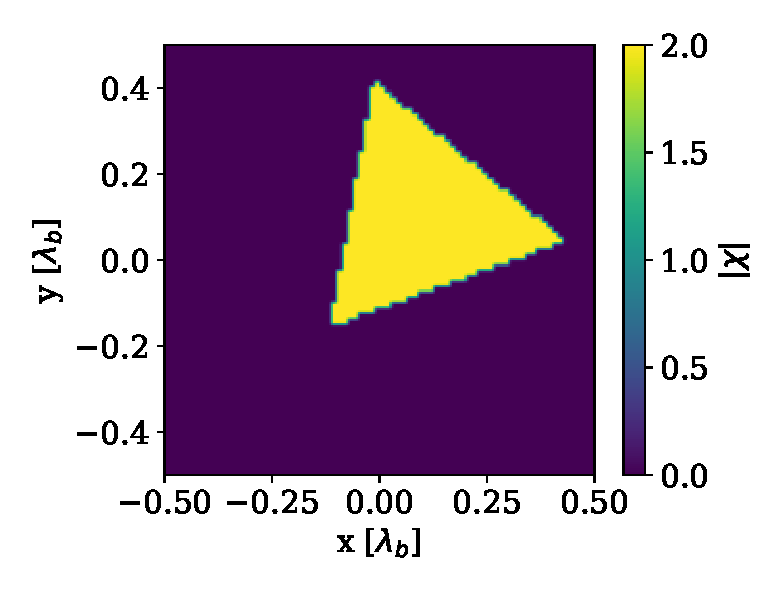
\includegraphics[width=.4\textwidth]{./figuras/transformation_original}} \hspace{.05\textwidth}
				\subfloat[]{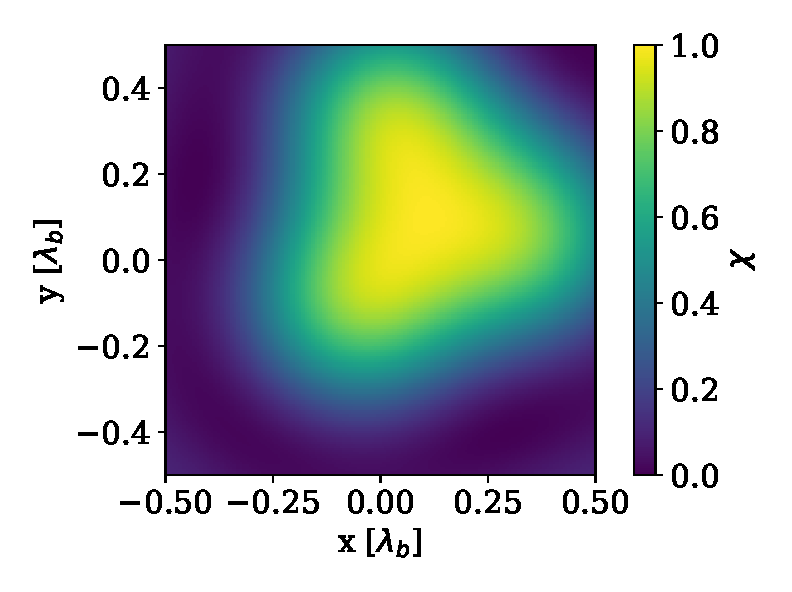
\includegraphics[width=.4\textwidth]{./figuras/transformation_thresholding}} \\
				\subfloat[]{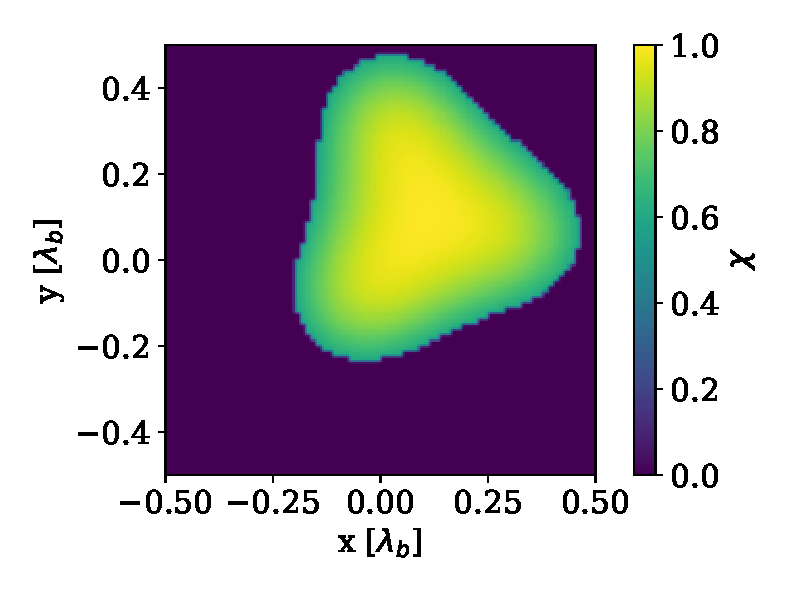
\includegraphics[width=.4\textwidth]{./figuras/transformation_multiplication}} \hspace{.05\textwidth}
				\subfloat[]{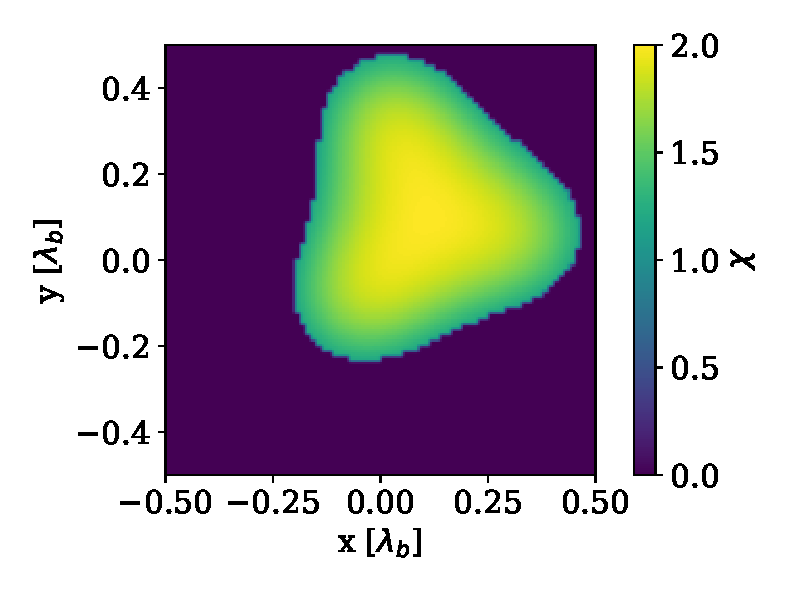
\includegraphics[width=.4\textwidth]{./figuras/transformation_final}}
				\caption[Example of the process of transforming a qualitative image into a quantitative one.]{Example of the process of transforming a qualitative image into a quantitative one: (a) ground-truth image; (b) image obtained by OSM ($\boldsymbol{\chi}^{norm}$); (c) image obtained after the thresholding process; and (d) final image obtained after the multiplication step.}
				\label{fig:proposed-methodology:surrogate:optimization:transformation}
			\end{figure}
			
			%The image $\boldsymbol{\chi}$ is also the diagonal elements of the contrast matrix $\boldsymbol{\bar{\chi}}$ in \eqref{eq:3:discretization:collocation:18}. Thus, the data equation error \eqref{eq:3:discretization:collocation:10} might be computed if the total electric field was also evaluated. Therefore, for a given scattered field data and the corresponding Green function matrix, the following bidimensional optimization problem might be defined:'
			The image $\boldsymbol{\chi}$ represents the diagonal elements of the contrast matrix $\boldsymbol{\bar{\chi}}$ mentioned in \eqref{eq:3:discretization:collocation:18}. Consequently, the data equation error \eqref{eq:3:discretization:collocation:10} can be calculated only if the total electric field is evaluated. Hence, a two-dimensional optimization problem can be defined based on a given scattered field data and its corresponding Green function matrix.
			\begin{align}
				T^*, \chi^{F*} =&~\arg\min f(T, \chi^F) \label{eq:proposed-methodology:surrogate:optimization:definition:objfun} \\
				& T\in[0, 1],~ \chi^{F} \in [\chi^F_{min}, \chi^F_{max}] \label{eq:proposed-methodology:surrogate:optimization:definition:bounds} 
			\end{align}
			
			\noindent where $ f(T, \chi^F)$ is the function that determines the data equation error based on the process of solving qualitatively the inverse problem through OSM and applying the transformation according \eqref{eq:proposed-methodology:surrogate:optimization:transformation}. Evidently, the total field must be computed for each pair $(T, \chi^F)$.
			
			%1. Um aspecto importante para qualquer problema de otimização são as características da função objetivo.			
			%2. No problema abordado, enquanto a variação da fator de multiplicação produz variações contínuas no erro da equação de dados, a variação do limiar não produz em pequena escala.
			%3. Uma vez que a imagem é uma representação discreta da função contraste, variações muito pequenas no operador de limiarização podem não causar mudança nenhuma na imagem resultante. Ou seja, se eu variar a variável T de modo que ela não alcance o menor valor de X dentro do objeto, a imagem não muda. Logo, o valor da função objetivo é constante nesse pequeno intervalo.
			Understanding the characteristics of the objective function is crucial for solving any optimization problem effectively. This is because the choice of the most appropriate algorithm depends on this information. Therefore, having knowledge of the objective function's properties is essential for selecting the best optimization method and achieving the desired outcome.
			
			In the optimization problem defined by \eqref{eq:proposed-methodology:surrogate:optimization:definition:objfun}-\eqref{eq:proposed-methodology:surrogate:optimization:definition:bounds}, varying the multiplication factor $\chi^F$ leads to continuous variations in the error of the data equation. However, varying the threshold $T$ does not produce a significant change on a small scale. This is due to the fact that the image is a discrete representation of the contrast function, and small variations in the thresholding operator may not cause any change in the resulting image. Hence, the value of the objective function remains constant in this small interval.
			
			%4. Este efeito ocorre em pequena escala. Ou seja, numa perspectiva macro da função objetivo, ela vai parecer suave e possivelmente até convexa. No entanto, quando se visualizarmos a superfície da função numa escala bem reduzida, notaremos discontinuidades na função. O que permite dizer que a função é multi-escala.
			%5. Isto pode trazer problemas para aplicação de métodos de otimização que se baseiam na informação da derivada. Isto porque a estimativa da derivada se dá pela avaliação da função num local vizinho da solução atual a qual está distante por um valor discreto de uma das variáveis. Logo, o ajuste desse valor discreto para perturbação da solução pode se tornar complicado pois, se o método estiver perto de uma discontinuidade, então o gradiente pode apontar para uma direção errada. Nesses casos, métodos sem-derivadas ou métodos baseados em população podem ser mais eficientes.
			Although this effect occurs on a small scale and the objective function appears smooth and convex from a macro perspective, when we visualize the surface of the function on a smaller scale, we will notice non-smoothness. This makes the function multi-scale and can create problems for optimization methods that depend on derivative information. When close to a roughness, the adjustment of the discrete value for perturbation of the solution might be complicated, making the gradient point in the wrong direction. Derivative-free methods or population-based methods may be more efficient in such cases.
			
			\begin{figure}[!h]
				\centering
				\subfloat[]{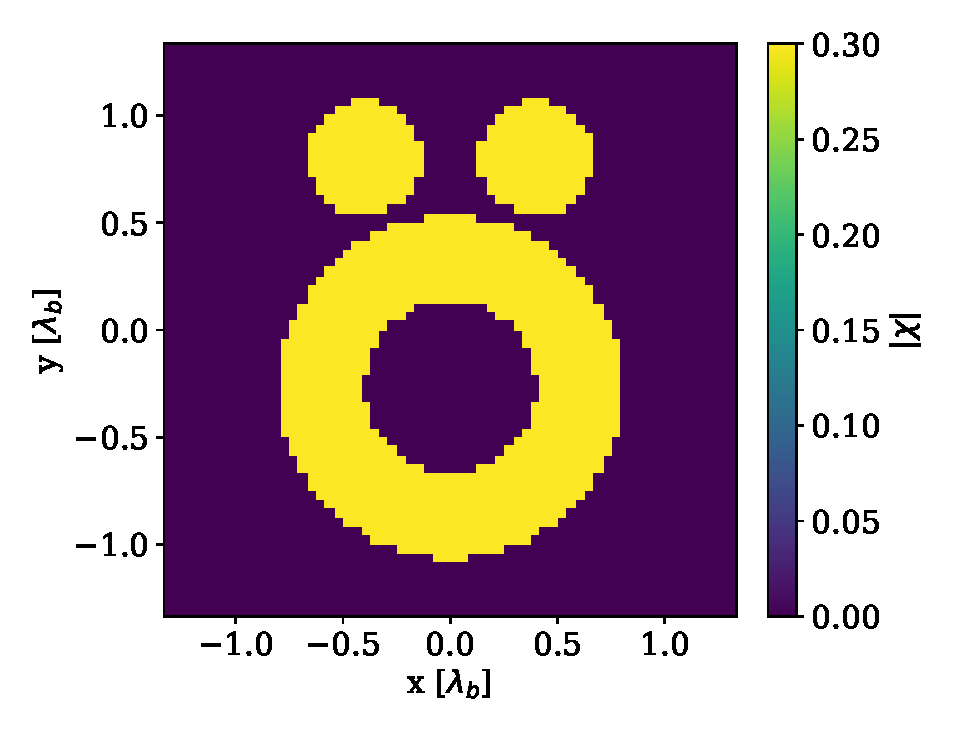
\includegraphics[width=.4\textwidth]{./figuras/objfun_groundtruth}\label{fig:proposed-methodology:surrogate:optimization:objfun:groundtruth}} \hspace{.05\textwidth}
				\subfloat[]{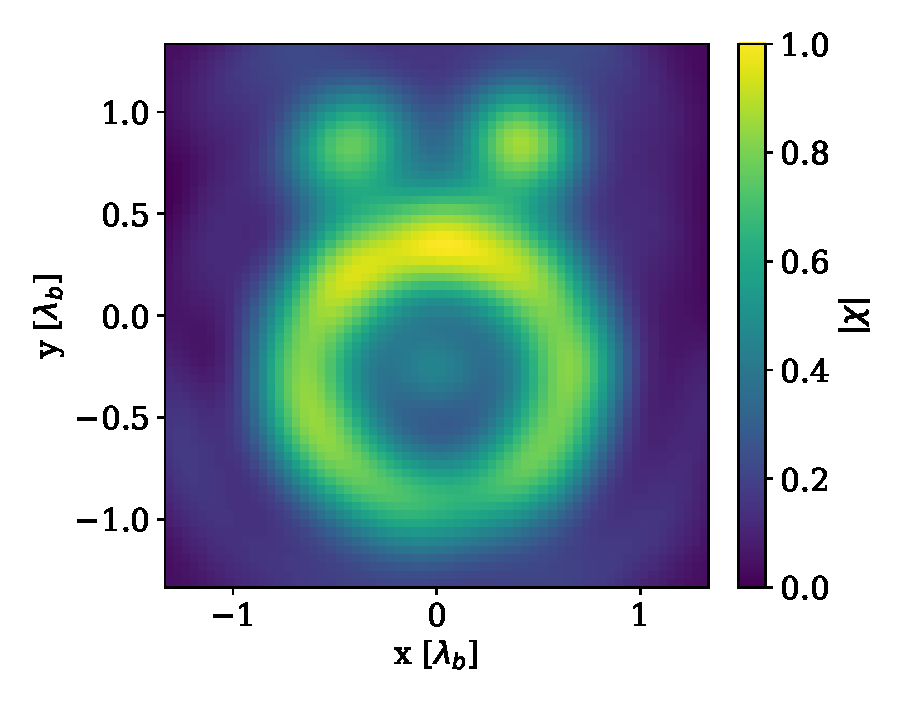
\includegraphics[width=.4\textwidth]{./figuras/objfun_qualitative}\label{fig:proposed-methodology:surrogate:optimization:objfun:qualitative}} \\
				\subfloat[]{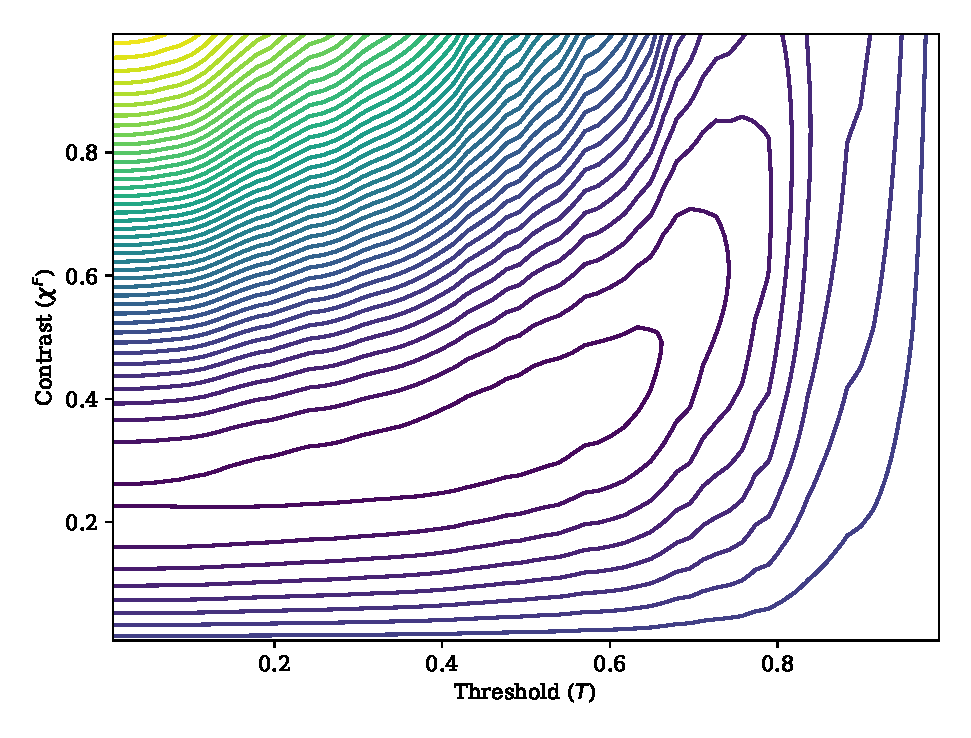
\includegraphics[width=.4\textwidth]{./figuras/objfun_surface}\label{fig:proposed-methodology:surrogate:optimization:objfun:surface}} \hspace{.05\textwidth}
				\subfloat[]{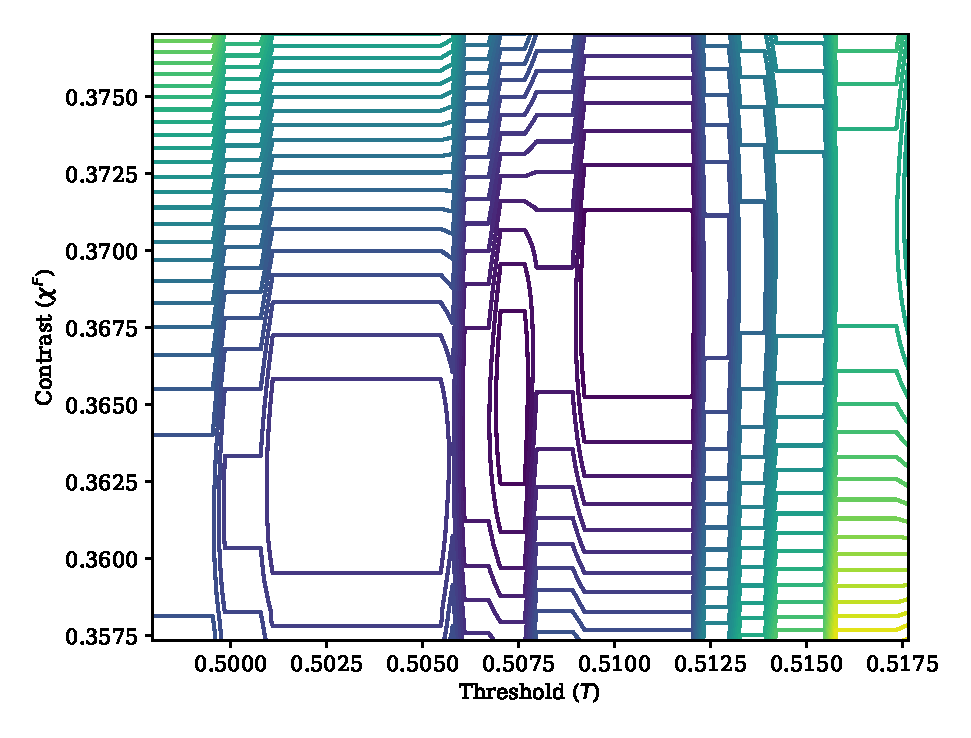
\includegraphics[width=.4\textwidth]{./figuras/objfun_nearoptimum}\label{fig:proposed-methodology:surrogate:optimization:objfun:nearoptimum}}
				\caption[Example of an objective function resulting from the transformation of the inversion problem into a two-dimensional optimization one.]{Example of an objective function resulting from the transformation of the inversion problem into a two-dimensional optimization one: (a) the ground-truth image; (b) the image obtained by OSM; (c) the surface obtained by the transformation of the inversion problem into a two-dimensional optimization one; and (d) a zoom over the region close to the optimum.}
				\label{fig:proposed-methodology:surrogate:optimization:objfun}
			\end{figure}
			
			%6. A figura 4 ilustra este problema. A figura 4(b) mostra a reconstrução a partir do método qualitativo para um teste representado pela figura 4(a). Na figura 4(c) vemos a superfície da função objetivo resultante da transformação do problema de inversão em um problema de otimização bidimensional. Como é possível notar, a superfície, numa perspectiva macro, parece bem suave. No entanto, quando ampliamos a imagem para perto do ótimo (figura 4(d)), vemos as discontinuidades no eixo da variável T.
			Figure \ref{fig:proposed-methodology:surrogate:optimization:objfun} illustrates this problem. Figure \ref{fig:proposed-methodology:surrogate:optimization:objfun:qualitative} shows the reconstruction from the qualitative method for a test represented by Figure \ref{fig:proposed-methodology:surrogate:optimization:objfun:groundtruth}. In Figure \ref{fig:proposed-methodology:surrogate:optimization:objfun:surface}, we see the surface of the objective function resulting from the transformation of the inversion problem into a two-dimensional optimization problem. The surface appears smooth from a macro perspective, but when we zoom in on the image close to the optimum (Figure \ref{fig:proposed-methodology:surrogate:optimization:objfun:nearoptimum}), we see the roughness on the $T$ variable axis.
			
			%7. Outra questão é que o valor ótimo do fator de multiplicação pode não coincidir com o valor exato do contraste da imagem, principalmente em casos de espalhadores homogêneos. Isto porque as variações de contraste dentro da região do objeto impossibilitam reconstruir com exatidão a imagem. Isto é possível obser pela figura 4(d). Uma alternativa para mitigar este efeito é assumir que o objeto é todo homogêneo e truncar os valores dentro da região do objeto pelo seu valor médio ou máximo.
			Another issue is that the optimal value of the multiplication factor may not coincide with the exact value of the image contrast, mainly in cases of homogeneous scatterers. This is because contrast variations within the object region make it difficult to accurately reconstruct the image. An alternative to mitigate this effect is to assume that the object is all homogeneous and truncate the values within the object's region by their average or maximum value.
			
			%8. Por fim, vale à pena frisar que a avaliação da função objetivo não é barata, uma vez que esta depende da execução do resolvedor direto para estimar o campo total correspondente. Logo, pode ser proibitivo a aplicação de um algoritmo de otimização que dependa de muitas avaliações.
			Finally, it is worth emphasizing that the evaluation of the objective function is not cheap since it depends on the execution of the direct resolver to estimate the corresponding total field. Therefore, applying an optimization algorithm that depends on many evaluations can be prohibitive.

		\subsection{Surrogate Models}\label{chap:proposed-methodology:surrogate:explanation}
			
			In many optimization problems, the objective function can be computationally expensive to evaluate, meaning that it takes a long time to compute the value of the function for a given set of input parameters. This can make it difficult to find good quality solutions, as it may take many iterations of the optimization algorithm to explore the search space thoroughly.
			
			Surrogate Models are approximations of the expensive objective function that are designed to reduce the computational cost of evaluating the objective function \citep{schonlau1997computer,mendes2013surrogate,sacks1989design}. A surrogate model is typically trained on a set of input-output pairs, where the inputs are the parameters of the optimization problem and the outputs are the value of the objective function for those parameters. The surrogate model learns to approximate the objective function using this training data, allowing it to make predictions about the value of the objective function for new sets of input parameters without actually evaluating the expensive objective function.
			
			Surrogate models can be used to speed up the convergence of optimization algorithms, as the surrogate model can be evaluated much more quickly than the expensive objective function. This means that the optimization algorithm can explore the search space more quickly, potentially finding good quality solutions in fewer iterations. Additionally, the use of surrogate models can reduce the number of evaluations of the expensive objective function, which can be a significant computational cost in some problems \citep{sobester2008engineering}.
			
			There are many different types of surrogate models, including regression models, neural networks, and Gaussian processes, among others. In this thesis, the Kriging model is considered since it is widely used in optimization problems \citep{emmerich2006single,zhao2011metamodeling,yang2019two} and it has shown slightly better performance in single-objective optimization problems \citep{valadao2020comparative}. 
			
			% The choice of surrogate model will depend on the specific problem and the available data. In some cases, it may be necessary to use multiple surrogate models or to combine surrogate models with other optimization techniques in order to achieve the best results.
		
		\subsection{Kriging Model}\label{chap:proposed-methodology:surrogate:kriging}
		
			Let $y : \mathbb{X} \subset \mathbb{R}^n \Rightarrow \mathbb{R}$ be an objective function for a given problem. A sample with $N$ solutions and their respective evaluations are $\mathbf{X} =  [\mathbf{x}^1, \cdots, \mathbf{x}^N]^T$ and $\mathbf{y} = [y(\mathbf{x}^1), \cdots, y(\mathbf{x}^N)]^T$, respectively. The Kriging model is a regression model where each observation of the objective function is treated as \citep{sacks1989design,schonlau1997computer,jones1998efficient}:
			\begin{equation}
				y(\mathbf{x}^i) = f(\mathbf{x}^i) + e(\mathbf{x}^i),~ i = 1, \cdots, N \label{eq:kriging:responsemodel}
			\end{equation}
		
			\noindent where $f(\mathbf{x}^i) = \mathbf{f}^T\boldsymbol{\alpha} = \sum\limits_{k=0}^d \alpha_kf_k(\mathbf{x}^i)$, $d\le N-1$, is a linear combination of the regression functions $f_k(\cdot)$ and $\alpha_k$, $k=0,\cdots,d$, are the corresponding coefficients; $e(\cdot)$ is a random normal variable with zero mean and variance $\Sigma^2$. Regression functions are similar to the trial functions presented in Section \ref{chap:methods:discretization}. In the scope of present subsection:
			\begin{equation}
				f_k(\mathbf{x}) = \prod\limits_{r=1}^n x_r^{q_r},~ q_r \in [0, Q],~ \sum\limits_{r=1}^n q_r \le Q \label{eq:kriging:trialfunctions}
			\end{equation}

			\noindent where $Q$ is the highest integer that satisfies $\frac{(n+Q)!}{Q!n!} < N-1$ \citep{zhao2011metamodeling}. The covariance of $e(\cdot)$ is assumed as:
			\begin{equation}
				Cov(e(\mathbf{x}^i), e(\mathbf{x}^j)) = \Sigma^2R(\boldsymbol{\theta},\mathbf{x}^i,\mathbf{x}^j) \label{eq:kriging:covariance}
			\end{equation}
		
			\noindent where $R(\cdot, \cdot, \cdot)$ is a Gaussian correlation function whose form is:
			\begin{equation}
				R(\boldsymbol{\theta},\mathbf{x}^i,\mathbf{x}^j) = \prod\limits_{r=1}^n e^{-\theta_r|x_r^i-x_r^j|^2} \label{eq:kriging:gaussiancorrelation}
			\end{equation}
		
			\noindent with $\boldsymbol{\theta} \in \mathbb{H}$, $\mathbb{H} = \left\{[\theta_1,\cdots,\theta_n]|\theta_r>0\forall r=1,\cdots,n\right\}$. Other correlation functions are also possible \citep{sacks1989design,mackay1998introduction}. However, \eqref{eq:kriging:gaussiancorrelation} is often used when the Kriging model is considered \citep{jin2005comprehensive,zhao2011metamodeling}. The parameters $\boldsymbol{\theta}$ are estimated based on the available sample and they mean the importance of each variable and how correlated they are.
			
			The optimal choice of $\boldsymbol{\theta}$, based on the sample data, is defined as the maximum likelihood estimator (MLE), where the likelihood funnction has the following form:
			\begin{equation}
				L(\boldsymbol{\theta}) = \frac{1}{\sqrt{(2\pi\Sigma^2)^N|\mathbf{R}|}}\mathrm{exp}\left(-\frac{1}{2\Sigma^2}(\mathbf{y}-\mathbf{F}\boldsymbol{\alpha})^T\mathbf{R}^{-1}(\mathbf{y}-\mathbf{F}\boldsymbol{\alpha})\right) \label{eq:kriging:mle}
			\end{equation}
		
			\noindent where $\mathbf{F}=[f_k(\mathbf{x}^i)]_{N\times(d+1)}$ and $\mathbf{R} = [R(\boldsymbol{\theta},\mathbf{x}^i,\mathbf{x}^j)]_{N\times N}$ are the regression and correlation matrices, respectively, with $i,j\in {1,\cdots, N}$ and $k\in {0,\cdots,d}$. For a given $\boldsymbol{\theta}$, the expressions:
			\begin{eqnarray}
				\boldsymbol{\hat{\alpha}} &=& \left(\mathbf{F}^T\mathbf{R}^{-1}\mathbf{F}\right)^{-1}\mathbf{F}^T\mathbf{R}^{-1}\mathbf{y} \label{eq:kriging:alphamle} \\
				\hat{\Sigma}^2 = \frac{1}{N} \left(\mathbf{y}-\mathbf{F}\boldsymbol{\hat{\alpha}}\right)^T\mathbf{R}^{-1}(\mathbf{y}-\mathbf{F}\boldsymbol{\hat{\alpha}}) \label{eq:kriging:sigma2mle}
			\end{eqnarray}
		
			\noindent provide the respective MLEs of $\boldsymbol{\alpha}$ and $\Sigma^2$. If \eqref{eq:kriging:alphamle} and \eqref{eq:kriging:sigma2mle} are used in \eqref{eq:kriging:mle}, then the optimal $\boldsymbol{\theta}$ is obtained through:
			\begin{equation}
				\arg\max\limits_{\boldsymbol{\theta}\in \mathbb{H}} \ln~L(\boldsymbol{\theta}) \label{eq:kriging:optimization}
			\end{equation}
		
			\noindent where:
			\begin{equation}
				\ln~L(\boldsymbol{\theta}) = -\frac{N}{2}\ln(2\pi) - N\ln(\hat{\Sigma}) - \ln(|\mathbf{R}|) - \frac{1}{2}
			\end{equation}
		
			By determining the optimal $\boldsymbol{\theta}$ through \eqref{eq:kriging:optimization}, the correlation matrix $\mathbf{R}$ is obtained and $\boldsymbol{\hat{\alpha}}$ and $\hat{\Sigma}^2$ are computed according to \eqref{eq:kriging:alphamle} and \eqref{eq:kriging:sigma2mle}, respectively. Then, for an untried input $\mathbf{x}$, the predicted evaluation and its mean squared error are, respectively:
			\begin{eqnarray}
				\hat{y}(\mathbf{x}) &=& \mathbf{f}^T\boldsymbol{\hat{\alpha}} + \mathbf{r}^T\mathbf{R}^{-1}(y-\mathbf{F}\boldsymbol{\hat{\alpha}}) \label{eq:kriging:prediction} \\
				\hat{s}^2(\mathbf{x}) &=& \hat{\Sigma}^2\left[1-\left(\mathbf{f}^T(\mathbf{x})+\mathbf{r}^T(\mathbf{x})\right) \begin{pmatrix} \mathbf{0} & \mathbf{F}^T \\ \mathbf{F} & \mathbf{R} \end{pmatrix}^{-1} \begin{pmatrix} \mathbf{f}(\mathbf{x}) \\ \mathbf{r}(\mathbf{x}) \end{pmatrix} \right]
			\end{eqnarray}
		
			\noindent where $\mathbf{r}^T(\mathbf{x}) = \left[R(\boldsymbol{\theta}, \mathbf{x}^1, \mathbf{x}), \cdots, R(\boldsymbol{\theta}, \mathbf{x}^N, \mathbf{x})\right]$ is the vector of correlation; $R(\boldsymbol{\theta}, \mathbf{x}^i, \mathbf{x})$ represents the correlation between $e(\cdot)$ at the sampled point $\mathbf{x}^i$ and $e(\cdot)$ at an untried $\mathbf{x}$, for $i=1,\cdots,N$. 
			
			Finally, such Kriging model is an interpolation model. Interestingly, when \eqref{eq:kriging:prediction} is evaluated at a point that belongs to the sample, then the prediction is the actual evaluation. This is due to the matching of $\mathbf{r}^T$ for the considered point with a line of the matrix $\mathbf{R}$.

		\subsection{Surrogate model-Assisted Algorithms}\label{chap:proposed-methodology:surrogate:algorithms}
		
			% 1. Na subseção 3.1, foi visto que a função-objetivo resultante da transformação do problema inversão em um de otimização bidimensional, além de ser multi-escala, é também cara computacionalmente. Estas características decorrem da não-suavidade do operador de limiarização e da necessidade de solução do problema direto para estimativa do erro.
			% 2. Uma alternativa para esses dois problemas é a substituição da função objetivo por um modelo substituto. Tendo em vista que o modelo substituto é um operador de interpolação, ele pode contornar o problema da micro-escala. Ou seja, reconstruir a função-objetivo pelas suas características macroscópicas através de um conjunto de pontos na superfície que não são muito próximos. O modelo substituto será uma função suave desde que use funções de base suaves. Além disso, a predição da avaliação da função objetivo é um processo muito mais barato do que a avaliação em si. Portanto, fica mais viável a aplicação de algoritmos de direção de busca e de população também.
			
			The chapter presented various aspects related to the proposed optimization problem and the use of surrogate models. Subsection \ref{chap:proposed-methodology:surrogate:optimization} showed how the inversion problem was transformed into a two-dimensional optimization problem. However, the obtained objective function is non-smooth and computationally expensive due to the non-smoothness of the thresholding operator and the need to solve the problem directly to estimate the data equation error. To address these challenges, one alternative is to use a surrogate model, which can reconstruct the objective function by considering its macroscopic characteristics through a set of surface points that are not too close together. The surrogate model works as an interpolation operator and can overcome the microscale problem, resulting in a smooth function when smooth basis functions are used. Additionally, predicting the objective function evaluation is less costly than evaluating it, making it feasible to apply search direction and population-based algorithms.
			
			% 3. De uma maneira geral, um algoritmo assistido por modelos substitutos dependem de, em primeiro lugar, obter uma amostra de pontos no espaço de busca com suas respectivas avaliações. Com essa amostra, o modelo substituto da função objetivo é construído. A partir daí, o processo de busca pode ser iniciado e, simulateamente, o modelo substituto é atualizado a partir de novas soluções encontradas e escolhidas para serem avaliadas pela função objetivo. Portanto, além das diferentes formas de obter o conjunto inicial, é possível explorar diferentes metodologias de busca e de atualização do modelo.
			In order to implement an algorithm assisted by surrogate models, the first step is to obtain a sample of points in the search space along with their respective evaluations. Based on this sample, the surrogate model of the objective function can be constructed. Once the surrogate model is obtained, the search process can begin, and the model can be updated with new solutions that are chosen to be evaluated by the objective function. Thus, in addition to the various methods for obtaining the initial set of points, it is also possible to explore different methodologies for searching and updating the surrogate model.
			
			% 4. Com relação às metodologias de obtenção da amostra inicial de soluções para o modelo substituto, uma forma trivial é a amostragem uniforme do espaço de busca. Ou seja, dados os intervalos das variáveis de decisão, são amostrados pontos equidistantes em cada eixo. No entanto, a abordagem mais tradicional é a Latin Hypercube Sampling (LHS) \cite{iman1981apporach}. It is a statistical method that generates quasi-random sampling distributions. It is widely used in computer experiments due to its simplicity and its projection properties in high-dimensional problems. To construct the LHS design, each variable dimension space is divided into n sections, where n represents the number of sampling points. Then, only one point is placed in each of the sections.
			One way to obtain the initial sample of solutions is through uniform sampling of the search space. This involves sampling equidistant points on each axis within the range of decision variables. However, the more traditional approach is Latin Hypercube Sampling (LHS) \cite{iman1981apporach}, which is a statistical method that generates quasi-random sampling distributions. LHS is widely used in computer experiments due to its simplicity and projection properties in high-dimensional problems. To construct the LHS design, the space of each variable dimension is divided into n sections, where n is the number of sampling points. Only one point is then placed in each section.

			
			% 5. Para ilustrar possíveis diferenças entre esses dois métodos de amostragem, foi simulado um problema de um espalhador de alto contraste (Figura 5a). Note que a função objetivo (Figura 5b)  é multimodal. A amostragem pelo método LHS resulta na superfície da Figura 5c, enquanto a obtida pela amostragem uniforme é apresentada na Figura 5d. Note que, na superfície obtida pelo LHS, existe uma barreira separando a região original do mínimo em duas. Nessa separação, não existe nenhuma amostra. Uma vez que o método LHS é estocástico, então cada amostragem pode resultar numa superfície diferente e regiões importantes podem ficar sem nenhuma amostra. Na amostragem uniforme, também não é garantido que uma região fique sem amostras. Principalmente se o número de amostras for baixo. Mas, com um número razoável de amostras, pode-se chegar a uma superfície com características mais parecidas principalmente quando o problema é bidimensional, como é o caso do exemplo da Figura 5. Portanto, para evitar os aspecto estocástico na amostragem, a metodologia uniforme será adotada sendo necessário escolher sempre um número adequado de amostras.
			To illustrate the differences between these two sampling methods, a high-contrast scatterer problem was simulated (Figure \ref{fig:proposed-methodology:surrogate:algorithms:samplings:groundtruth}), resulting in a multimodal objective function (Figure \ref{fig:proposed-methodology:surrogate:algorithms:samplings:objfun}. Sampling by the LHS method resulted in a surface with a barrier separating the original minimum region in two, in which there was no sample (Figure \ref{fig:proposed-methodology:surrogate:algorithms:samplings:objfun}). Since the LHS method is stochastic, each sampling can result in a different surface, and important regions can be left without any samples. Uniform sampling can also result in regions running out of samples, especially if the number of samples is low. However, with a reasonable number of samples, a surface with similar characteristics can be obtained, especially in two-dimensional problems, as it is shown in Figure \ref{fig:proposed-methodology:surrogate:algorithms:samplings:uniform}. Therefore, to avoid the stochastic aspect of sampling, a uniform methodology is adopted, and it is always necessary to choose an adequate number of samples.

			\begin{figure}[!h]
				\centering
				\subfloat[]{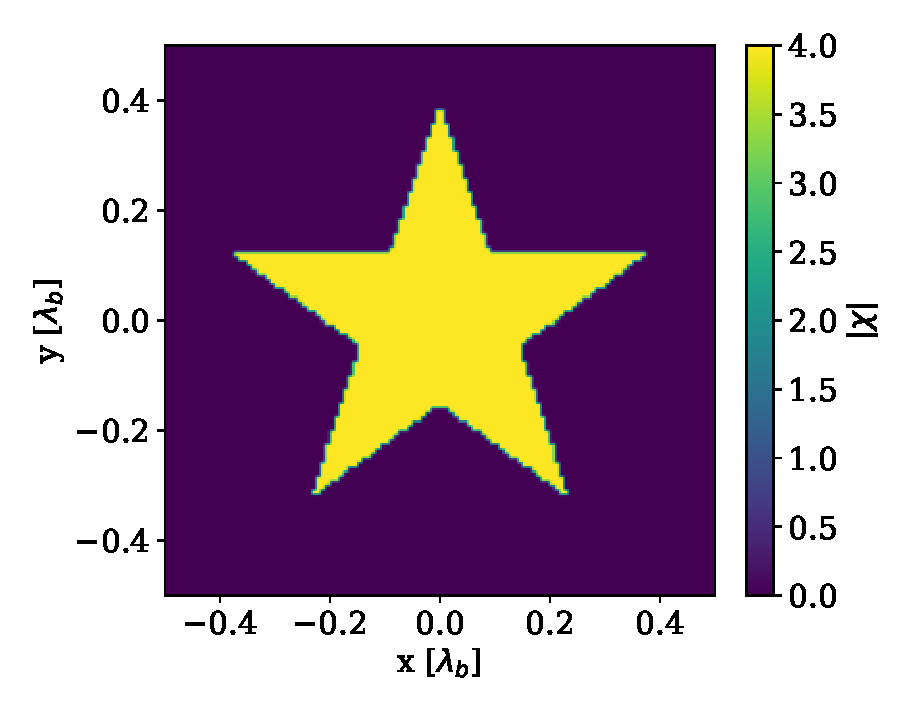
\includegraphics[width=.4\textwidth]{./figuras/samplings_groundtruth}\label{fig:proposed-methodology:surrogate:algorithms:samplings:groundtruth}} \hspace{.1\textwidth}
				\subfloat[]{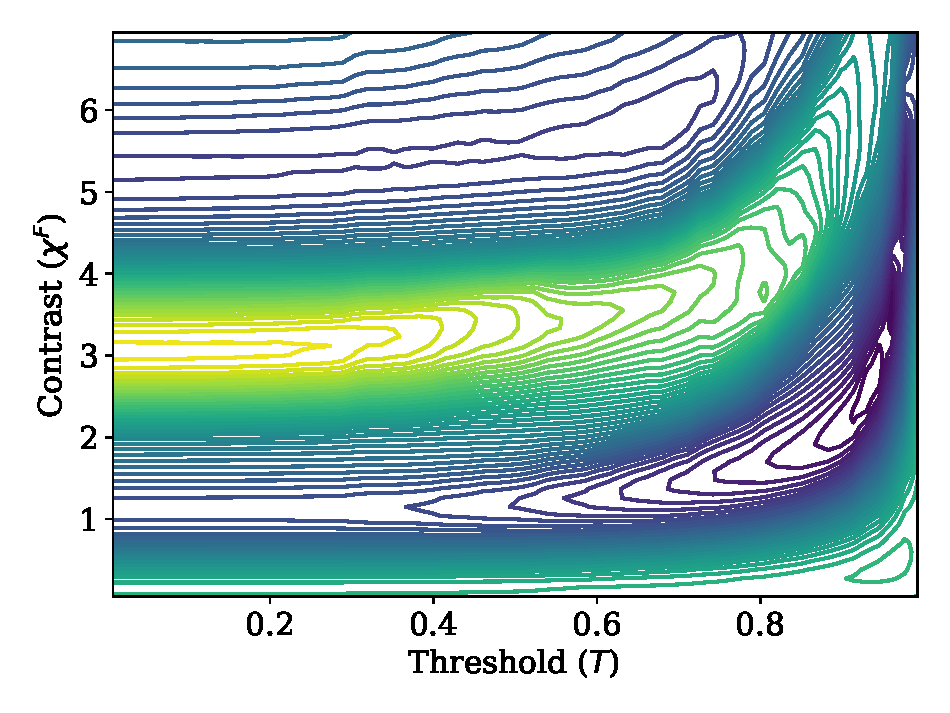
\includegraphics[width=.4\textwidth]{./figuras/samplings_objfun}\label{fig:proposed-methodology:surrogate:algorithms:samplings:objfun}} \\
				\subfloat[]{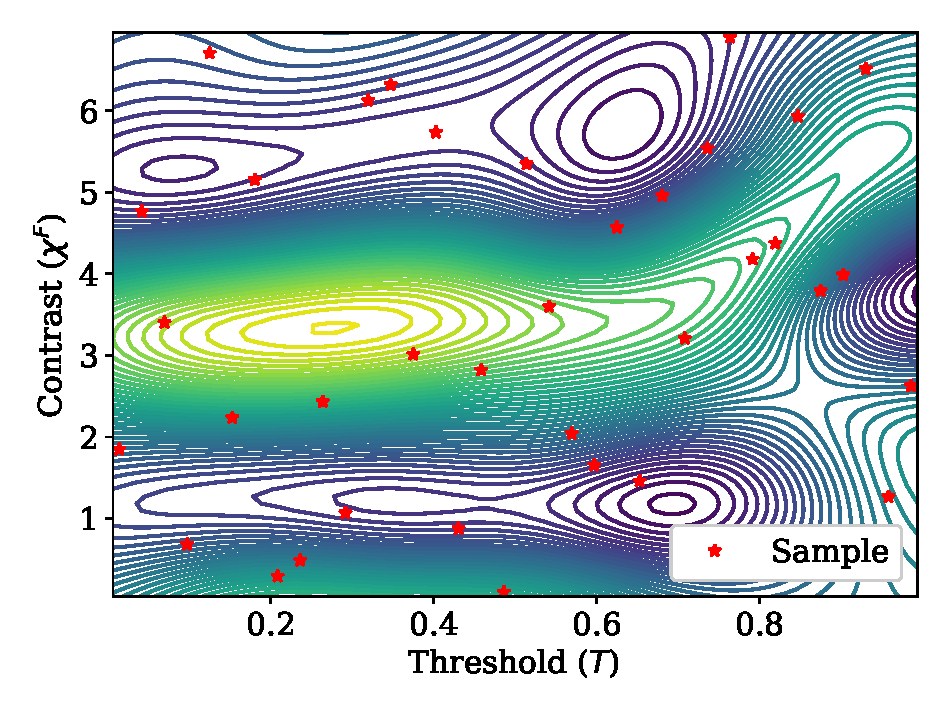
\includegraphics[width=.4\textwidth]{./figuras/samplings_lhs}\label{fig:proposed-methodology:surrogate:algorithms:samplings:lhs}} \hspace{.1\textwidth}
				\subfloat[]{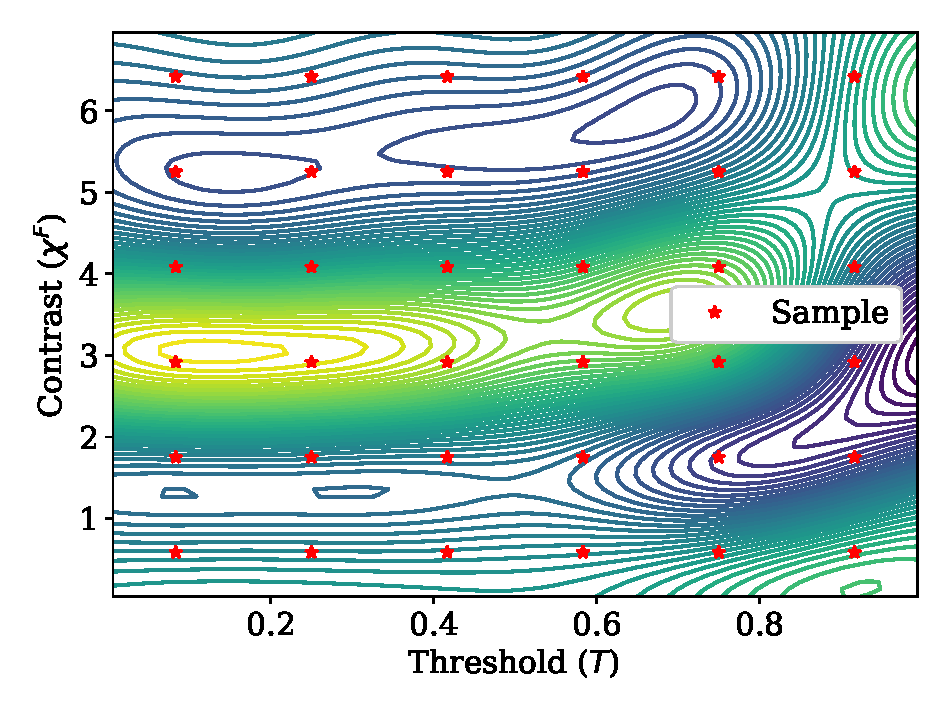
\includegraphics[width=.4\textwidth]{./figuras/samplings_uniform}\label{fig:proposed-methodology:surrogate:algorithms:samplings:uniform}}
				\caption[Comparison of Latin Hypercube Sampling and Uniform Sampling methods for strong scatterer instance.]{Comparison of Latin Hypercube Sampling and Uniform Sampling methods for strong scatterer instance: (a) the ground-truth image; (b) the surface of the corresponding objective-function; (c) the predicted surface obtained by LHS; (d) the predicted surface obtained by uniform sampling.}
				\label{fig:proposed-methodology:surrogate:algorithms:samplings}
			\end{figure}
			
			Surrogate Model-Assisted Evolutionary Algorithms (SAEAs) are a popular approach  \citep{emmerich2006single,liu2014gaussian}. Despite the various possible formulations of SAEAs \citep{buche2005accelerating}, they all share the same general structure \citep{he2023review}. In Figure \ref{fig:proposed-methodology:surrogate:algorithms:saeaflowchart}, the general flowchart is illustrated. The main cycle of the algorithm is initiated after the initial set of solutions is obtained and the surrogate model is built. In each generation of the cycle, the current surrogate-model is utilized to evaluate the fitness values of individuals instead of the real objective-function. An evolutionary algorithm is then employed to continually search for the optimal solution of the problem. Meanwhile, high-quality individuals are selected to update the sample and, therefore, are evaluated according the true objective function to update the surrogate-model \citep{zhou2007combining,liu2014gaussian,sun2017surrogate}. These operations are repeated until the termination condition is met \citep{jin2005comprehensive}.
			
			\begin{figure}[!h]
				\centering
				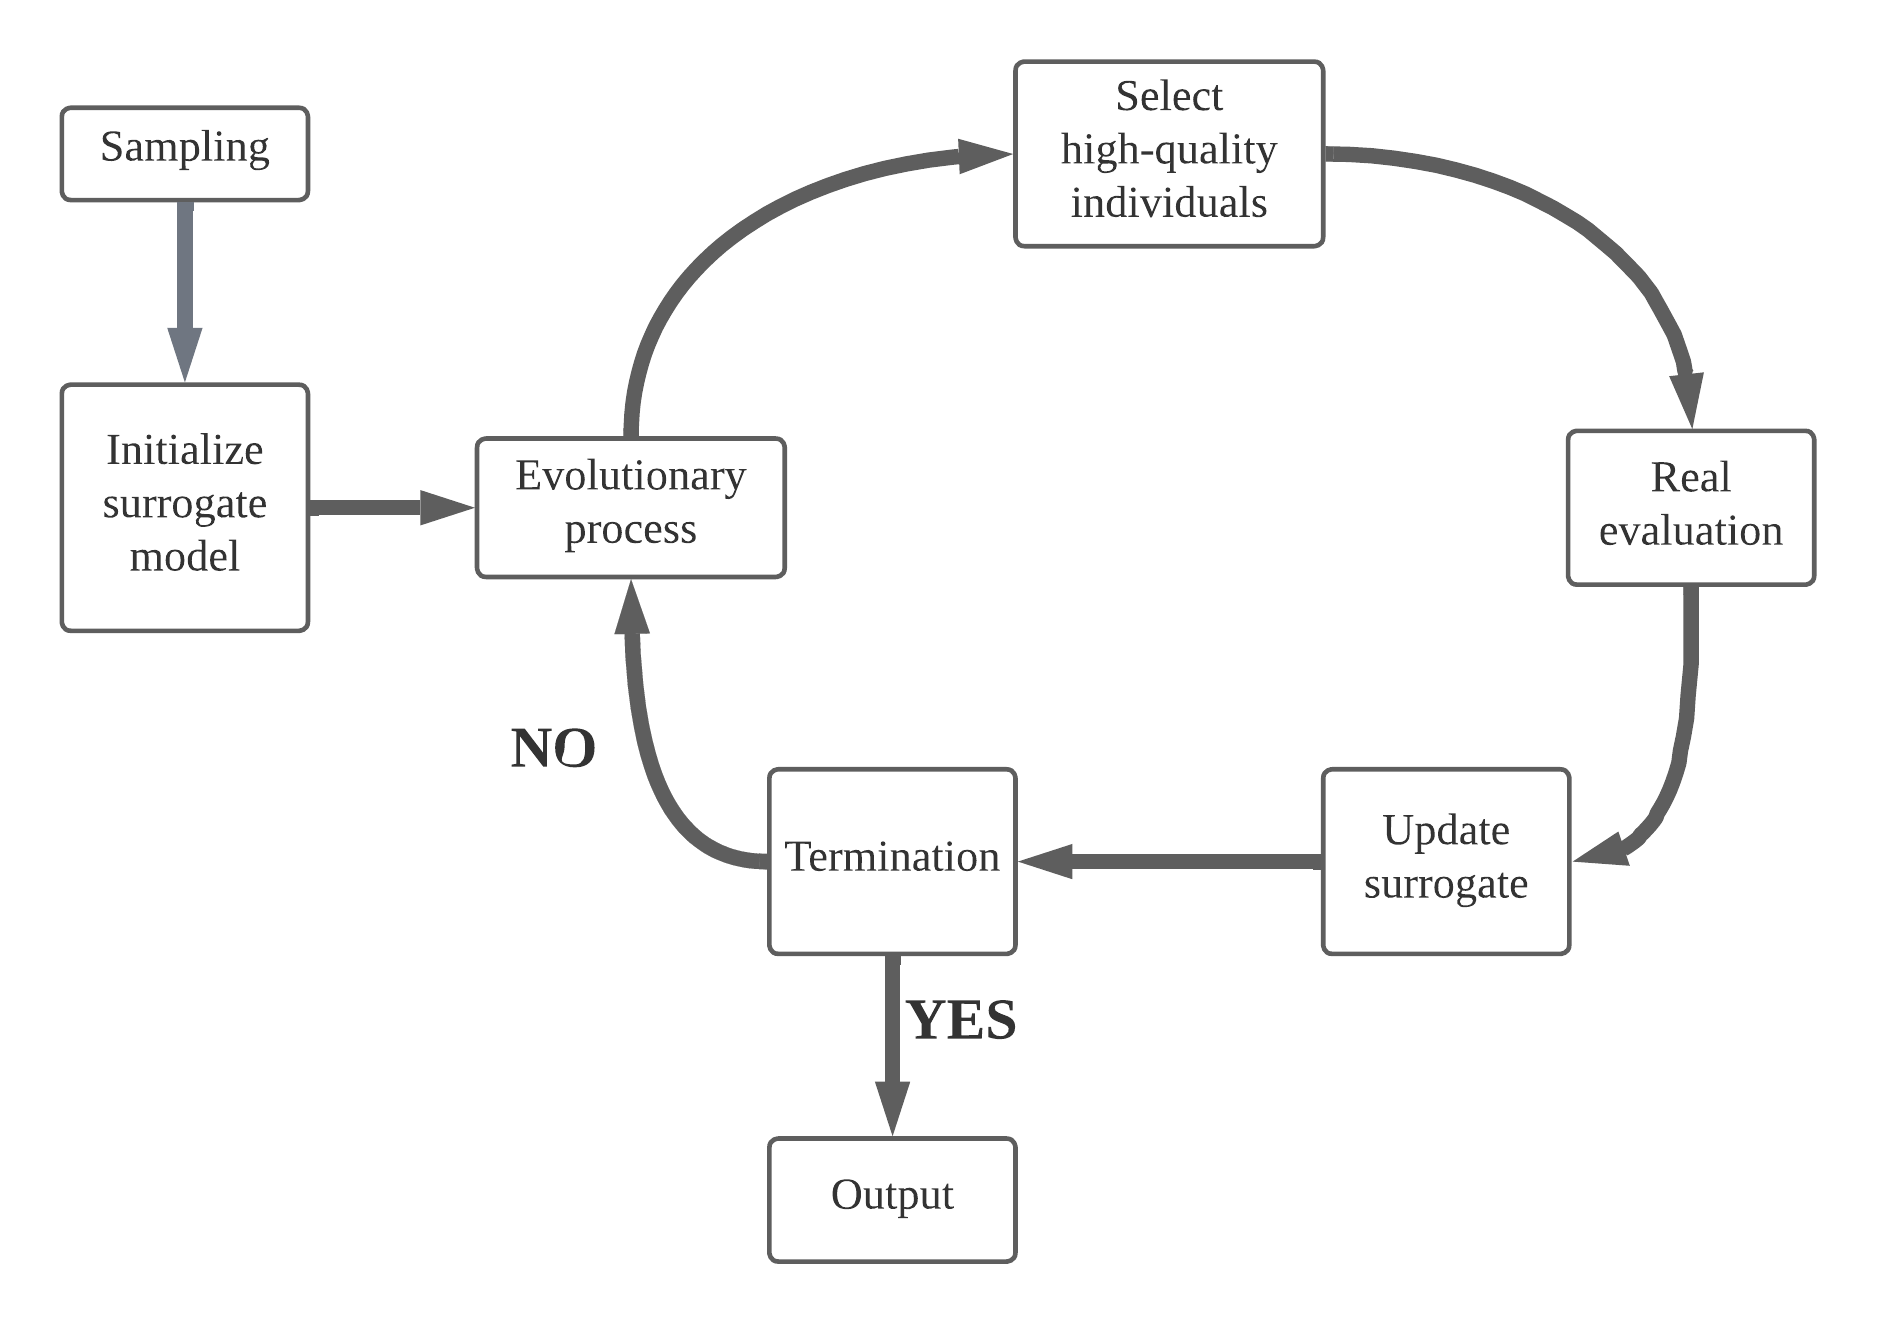
\includegraphics[width=.8\textwidth]{./figuras/saeaflowchart}
				\caption[The basic flowchart of SAEAs.]{The basic flowchart of SAEAs.}
				\label{fig:proposed-methodology:surrogate:algorithms:saeaflowchart}
			\end{figure}
			
			In surrogate model-assisted optimization algorithms, it is not only population-based algorithms that can be used. Since the surrogate model is constructed from smooth basis functions, it is also possible to use search direction methods based on derivatives. Once the surrogate model is built, a local optimum of the predicted surface can be obtained by applying such methods to a given starting point. This local optimum is then evaluated based on the true objective function, and the surrogate model is updated with this new sample. This process is then repeated with the final solution from the previous iteration as the new starting point. Given that the objective function is reasonably sampled early on, such a method could converge to the optimum solution. A stopping criterion for this method could be consecutive iterations in which the optimal solution does not change. Different formulations can be explored for choosing the first starting point of the search direction method. This can be especially important in multimodal problems, such as the one addressed in this thesis.
		
			In this thesis, three SAEAs approaches are considered. Their differences are the way in which the population is initialized and the way in which the high-quality individuals are selected for updating the model. In addition, two Surrogate model-Assisted Descent Methods (SADMs) are also proposed. Their main difference is the approach for obtaining an initial solution. The next subsubsections describe all of them.
		
			\subsubsection{SAEA1}\label{chap:proposed-methodology:surrogate:algorithms:saea1}
			
				The first SAEA approach is inspired in \citep{salucci2022learned}. After initializing the surrogate model, the population is initialized by simply sampling random points in the search space following the uniform distribution. Their fitness are computed by the surrogate model prediction. Then, the algorithm executes a single iteration of the chosen evolutionary process. After the new population is selected\footnote{The elitism strategy is considered, i.e., the best solution among the parent and offspring populations is preserved for the next generation.}, the current best solution is compared against the sample. If it differs from all available solutions in the sample, its fitness is updated according to the real objective function and it is added to the sample. The model is trained again and all the individuals in the current population are re-evaluated according the updated surrogate model. The cycle repeats and this process continues until the stop criterion is met, at which point the algorithm returns the best solution in the sample. The pseudo-code presented in Algorithm \ref{alg:saea1} outlines this process.
				
				Overall, the following observations are drawn for the considered algorithm:
				\begin{itemize}
					\item The sample contains the initial solution and the best individuals discovered throughout the generations.
					\item The total number of evaluations of the true objective function is not greater than the sum of the number of initial samples and the number of generations.
					\item The offspring population is created using the DE/best/1 operator, and the F factor is randomly selected from a predetermined range.
					\item In addition, a local search step based on a Descent Method is added and performed after a fixed number of generations, which distinguishes this process from the one proposed by \cite{salucci2022learned}.
				\end{itemize}
				
				\begin{algorithm}[!h]
					\caption[Explanation of the functioning of the SAEA1 algorithm.]{The SAEA1 algorithm.}
					\label{alg:saea1}
					\KwIn{Scattered field data, discretization configuration, lower and upper bounds for $\chi^F$ and $T$, number of initial sampled solutions, population size}
					\KwOut{Contrast image.}
					Solve qualitatively the problem and obtain the normalized contrast image.\\
					Sample solutions within the search space uniformly in the defined interval of $\chi^F$ and $T$.
					Evaluate the sampled solutions.\\
					Evaluations $\leftarrow$ number of initial sampled solutions.\\
					Build and train the surrogate model based on the sample.\\
					Initialize a population of individuals by randomizing $\chi^F$ and $T$ values following the uniform distribution.\\
					Set their fitness according to their corresponding prediction obtained by the surrogate model.\\
					\While{stopping criteria is not met}{
						Generate a offspring population based on the DE/best/1 operator.\\
						Evaluate the offspring based on the surrogate model.\\
						Selected the new population considering the union of parents and offspring individuals by Binary Tournament and preserving the best solution among them (elitism).\\
						\If{the local search has not been executed in the last $N_{LS}$ generations}{
							Perform a local search using a Steepest Descent algorithm considering the current best solution as initial guess and the surrogate model as objective function.\\
							\If{the returned solution by the local search is better}{
								Update the current best solution.\\
							}	
						}
						\If{the current best solution is not equal to any other in the sample}{
							Evaluate the current best solution according the objective function.\\
							Evaluations $\leftarrow$ evaluations + 1\\
							Add the current best solution to the sample.\\
							Train the surrogate model.\\
							Re-evaluate the population using the updated surrogate model.\\
						}
					}
				\end{algorithm}
			
			\subsubsection{SAEA2}\label{chap:proposed-methodology:surrogate:algorithms:saea2}
				
				The second approach is inspired in the one proposed by \cite{valadao2020comparative}. The approach for selection and mutation in this algorithm differs from the typical prediction model-based population evaluation implemented in SAEA1. Instead, individual evaluation using the real function serves as the criterion for selection. The mutation strategy is also distinct, with mutation vectors calculated based on solutions stored in an archive. The archive is initially populated with the best solutions from the samples and is updated in each generation with the best $N_A$ solutions from the updated sample. Each offspring-individual is generated from a sub-selection of solutions, generated and evaluated by the surrogate model. The sub-selection generates a set of solutions, and the one with the best value for the prediction of the objective function is selected as the offspring. Then, its fitness is updated according the real objective function. The pseudo-code presented in Algorithm \ref{alg:saea2} outlines this process.
				
				In practice, the described algorithm leads to the following observations:
				\begin{itemize}
					% \item A amostra de soluções é sempre atualizada com as melhores soluções encontradas até geração atual. Logo, soluções com avaliaçõs ruins são retiradas de modo que o modelo prioriza mais a reconstrução da região mais promissora.
					\item The sample solutions are continuously updated with the best solutions found up to the current generation. This means that sampled solutions with the worst evaluations are removed to prioritize the reconstruction of the most promising region.
					% \item A cada geração, o número de avaliações aumenta com o tamanho da população. Portanto, este algoritmo tende a gastar mais avaliações para convergir.
					\item The number of evaluations increases with each generation in proportion to the population size, causing this algorithm to require more evaluations to converge.
					% \item Os mesmos operadores de mutação e de busca local foram aplicados nesta versão do algoritmo.
					\item The current version of the algorithm applies the same mutation and local search operators in each iteration.
				\end{itemize}
    
				\begin{algorithm}[!h]
					\caption[Explanation of the functioning of the SAEA2 algorithm.]{The SAEA2 algorithm.}
					\label{alg:saea2}
					\KwIn{Scattered field data, discretization configuration, lower and upper bounds for $\chi^F$ and $T$, number of initial sampled solutions, population size}
					\KwOut{Contrast image.}
					Solve qualitatively the problem and obtain the normalized contrast image.\\
					Sample solutions within the search space uniformly in the defined interval of $\chi^F$ and $T$.
					Evaluate the sampled solutions.\\
					Evaluations $\leftarrow$ number of initial sampled solutions.\\
					Build and train the surrogate model based on the sample.\\
					Initialize a population of individuals by selecting the $p$ best solutions from the sample.\\
					Store in the archive the best $N_A$ solutions.\\
					\While{stopping criteria is not met}{
						Generate $k$ solutions for each one in the population based on the DE/best/1 operator and evaluate them according to the surrogate model.\\
						For each group of $k$ solutions, selects the best, evaluate it according to the real function and set it as offspring individual.\\
						Evaluations $\leftarrow$ evaluations $+$ population size.\\
						Selected the new population considering the union of parents and offspring individuals by Binary Tournament and preserving the best solution among them (elitism).\\
						\If{the local search has not been executed in the last $N_{LS}$ generations}{
							Perform a local search using a Steepest Descent algorithm considering the current best solution as initial guess and the surrogate model as objective function.\\
							\If{the returned solution by the local search is better}{
								Update the current best solution.\\
							}	
						}
						\If{the current best solution is not equal to any other in the sample}{
							Add the current best solution to the sample.\\
							Train the surrogate model.\\
						}
						Update the archive with the $N_A$ best solutions in the sample.\\
					}
				\end{algorithm}
	
			\subsubsection{SAEA3}\label{chap:proposed-methodology:surrogate:algorithms:saea3}
			
				% A principal vantagem do SAEA1 é gastar somente uma avaliação por geração. Já a principal do SAEA2 é considerar um arquivo de melhores soluções como indivíduos-pais no momento da mutação. Estas duas características podem ser combinadas numa formulação híbrida, a SAEA3, na qual a população de indivíduos pais e filhos continua sendo avaliada pelo modelo substituto, ao passo que os vetores de mutação são gerados considerando um arquivo com as melhores soluções da amostra. Dessa forma, apenas a melhor solução da geração é avaliada pela função real. Desta forma, um número alto de gerações que o SAEA2 pode ser considerado e os indivíduos filhos tendem a herdar mais características das melhores soluções.
				SAEA1 has the main advantage of spending only one evaluation per generation, while SAEA2 has the advantage of considering an archive of best solutions as parents during mutation. The features of these two algorithms can be combined in a hybrid formulation, called SAEA3, where the population of parent and offspring individuals is evaluated by the surrogate model, and mutation vectors are generated based on a file with the best sample solutions. As a result, only the best solution of the generation is evaluated by the actual function. This approach enables SAEA3 to have a high number of generations, similar to SAEA1, while the offspring individuals tend to inherit more characteristics of the best solutions (exploitation), similar to SAEA2. The same mutation and local search operators in each iteration. The pseudo-code presented in Algorithm \ref{alg:saea3} outlines this process.
				
				\begin{algorithm}[!h]
					\caption[The SAEA3 algorithm.]{Explanation of the functioning of the SAEA3 algorithm.}
					\label{alg:saea3}
					\KwIn{Scattered field data, discretization configuration, lower and upper bounds for $\chi^F$ and $T$, number of initial sampled solutions, population size}
					\KwOut{Contrast image.}
					Solve qualitatively the problem and obtain the normalized contrast image.\\
					Sample solutions within the search space uniformly in the defined interval of $\chi^F$ and $T$.
					Evaluate the sampled solutions.\\
					Evaluations $\leftarrow$ number of initial sampled solutions.\\
					Build and train the surrogate model based on the sample.\\
					Initialize a population of individuals by selecting the $p$ best solutions from the sample.\\
					Store in the archive the best $N_A$ solutions.\\
					\While{stopping criteria is not met}{
						Generate $k$ solutions for each one in the population based on the DE/best/1 operator and evaluate them according to the surrogate model.\\
						For each group of $k$ solutions, selects the best and set it as offspring individual.\\
						Selected the new population considering the union of parents and offspring individuals by Binary Tournament and preserving the best solution among them (elitism).\\						
						\If{the local search has not been executed in the last $N_{LS}$ generations}{
							Perform a local search using a Steepest Descent algorithm considering the current best solution as initial guess and the surrogate model as objective function.\\
							\If{the returned solution by the local search is better}{
								Update the current best solution.\\
							}	
						}
						\If{the current best solution is not equal to any other in the sample}{
							Evaluate the current best solution according the objective function.\\
							Evaluations $\leftarrow$ evaluations + 1\\
							Add the current best solution to the sample.\\
							Train the surrogate model.\\
							Re-evaluate the population using the updated surrogate model.\\
						}
						Update the archive with the $N_A$ best solutions in the sample.\\
					}
				\end{algorithm}
			
			\subsubsection{SADM1}\label{chap:proposed-methodology:surrogate:algorithms:sadm1}
			
				% 1. Os algoritmos evolutivos podem explorar todo o espaço de busca, uma vez que são baseados em uma população de soluções.
				% 2. Quando um operador de busca local é aplicado sobre a atual melhor solução, o desempenho pode melhorar uma vez que se realiza uma busca mais intensa sobre uma solução potencial.
				% 3. O processo de amostragem do espaço de busca feito para construir o modelo substituto inicial pode ser pensado como uma população de soluções. Desta forma, se essa amostragem for razoavelmente ampla, a bacia de atração com maior potencial tem boas chances de ser amostrada. Nessas condições, podemos aplicar diferentes estratégias para escolher um ponto inicial e aplicar um algoritmo de direção de busca sobre o modelo substituto.
				% 4. Obviamente, a melhor solução encontrada pode não estar tão próxima do ótimo global. No entanto, esta pode ser avaliada de acordo com a função real e adicionada ao conjunto de amostras para atualizar o modelo.
				% 5. Logo, se esse processo for repetido iterativamente, o algoritmo tenderá a convergir para um local quando a soluções ótimas encontradas em um conjunto de iterações forem idênticas ou muito próximas.
				% 6. A grande questão é então como escolher a solução inicial que vai dar início ao processo iterativo de otimização.
				% 7. Uma possível estratégia é executar um algoritmo evolutivo considerando o modelo substituto inicial e tomar como solução inicial do processo iterativo a melhor solução encontrada pelo algoritmo evolutivo. Assim, uma busca global é feita e o processo iterativo tende a se concentrar na região da melhor bacia de atração disponível na primeira construção do modelo.
				
				Evolutionary algorithms are powerful optimization techniques based on a population of solutions. They are capable of exploring the entire search space (exploration), and when combined with local search operators, performance can improve significantly due to the exploitation of a potential solution. The initial surrogate model construction can be seen as a population of solutions, which, if sampled broadly, can cover the most promising region of the search space. Different strategies can be applied to choose a starting point and apply a steepest descent algorithm on the surrogate model.
				
				The best solution found may not necessarily be close to the global optimum, but it can be evaluated against the actual function and added to the sample set to update the model. By repeating this process iteratively, the algorithm will tend to converge to a location when the optimal solutions found in a set of iterations are identical or very close. However, the question of how to choose the initial solution that will start the iterative optimization process remains.
				
				One possible strategy is to run an evolutionary algorithm considering the initial surrogate model and take the best solution found as the initial solution of the iterative process. This way, a global search is performed, and the iterative process tends to focus on the region of the best basin of attraction available in the first construction of the model. Such an approach will be denoted as SADM1 where the initials stand for Surrogate-model Assisted Descent Method. The pseudo-code presented in Algorithm \ref{alg:sadm1} outlines this process.
				
				Overall, the following observations are drawn for the considered algorithm:
				\begin{itemize}
					\item The evolutionary algorithm employed to determine an initial guess is the Differential Evolution with the following formulation: DE/best/1/bin \citep{rocca2011differential}.
					\item The employed descent method is the L-BFGS-B algorithm which is a limited-memory version of Broyden-Fletcher-Goldfarb-Shanno (BFGS) algorithm for boundary constrained optimization \citep{byrd1995limited,zhu1997algorithm}.
				\end{itemize}
				
				\begin{algorithm}[!h]
					\caption[Explanation of the functioning of the SADM1 algorithm.]{The SADM1 algorithm.}
					\label{alg:sadm1}
					\KwIn{Scattered field data, discretization configuration, lower and upper bounds for $\chi^F$ and $T$, number of initial sampled solutions, population size}
					\KwOut{Contrast image.}
					Solve qualitatively the problem and obtain the normalized contrast image.\\
					Sample solutions within the search space uniformly in the defined interval of $\chi^F$ and $T$.
					Evaluate the sampled solutions.\\
					Evaluations $\leftarrow$ number of initial sampled solutions.\\
					Build and train the surrogate model based on the sample.\\
					Run an evolutionary algorithm considering the surrogate model as objective function and take the best solution as current solution.\\
					Evaluate the current solution according the true objective function, add it to the sample and retrain the model.\\
					\While{stopping criteria is not met}{
						Run the descent method considering the current solution as initial guess and optimizing the predicted surface.\\
						Evaluate the returned solution according the true objective function.\\
						Evaluations $\leftarrow$ evaluations + 1\\
						\If{the returned solution is not equal to any other in the sample}{
							Add the current best solution to the sample.\\
							Train the surrogate model.\\
						}
						\If{the returned solution is better than the current one}{
							Set the current solution as the returned by the last call of the descent optimization.\\
						}
					}
				\end{algorithm}
	
			\subsubsection{SADM2}\label{chap:proposed-methodology:surrogate:algorithms:sadm2}
			
				% 1. Ao invés de determinar o ponto inicial para o processo iterativo do SADM através da utilização de um algoritmo evolucionário, uma alternativa mais simples é escolher a melhor amostra como ponto de partida. Ou seja, após amostrar o espaço de busca, o processo iterativo começa assumindo como solução atual a melhor amostra do modelo.
				% 2. Além de mais simples, uma vantagem é evitar a possibilidade de convergir para uma outra bacia de atração diferente da de mínimo global quando esta estiver perto da melhor amostra. Em outras palavras, considerando a superfície gerada pelo modelo substituto, o algoritmo evolutivo não garante a convergência para o mínimo globa, uma vez que é estocástico. No entanto, se por um acaso o mínimo global estiver próximo da melhor amostra, o que é bem possível, então a primeira iteração do SADM convergirá para esse local.
				% 3. É claro que, se a superfície não for bem amostrada no começo, então poder ser o processo convirja para uma região diferente da do ótimo global da função real. E isso pode ser mais complicado em casos de espalhadores fortes, onde a função objetivo tende a ser multi-modal. Mas quando a função objetivo é menos complexa, então essa estratégia pode ser bem eficiente.
				
				Rather than determining the starting point for the SADM iterative process using an evolutionary algorithm, a simpler alternative is to choose the best sample as the starting point. That is, after sampling the search space, the iterative process starts assuming the best sample of the model as the current solution. In addition to being simpler, an advantage is to avoid the possibility of converging to another basin of attraction different from the global minimum when this is close to the best sample. In other words, considering the surface generated by the surrogate model, the evolutionary algorithm does not guarantee convergence to the global minimum, since it is stochastic. However, if by chance the global minimum is close to the best sample, which is quite possible, then the first iteration of SADM will certainly converge to that location. Of course, if the surface is not sampled well at the beginning, then the process may converge to a region other than the global optimum of the real function. And this can be more complicated in cases of strong scatterers, where the objective function tends to be multi-modal. But when the objective function is less complex then this strategy can be quite efficient. This approach will be denoted as SADM2 and its pseudo-code is shown in Algorithm \ref{alg:sadm2}. The L-BFGS-B algorithm will be used in a similar manner to SADM1.
				
				\begin{algorithm}[!h]
					\caption[Explanation of the functioning of the SADM2 algorithm.]{The SADM2 algorithm.}
					\label{alg:sadm2}
					\KwIn{Scattered field data, discretization configuration, lower and upper bounds for $\chi^F$ and $T$, number of initial sampled solutions, population size}
					\KwOut{Contrast image.}
					Solve qualitatively the problem and obtain the normalized contrast image.\\
					Sample solutions within the search space uniformly in the defined interval of $\chi^F$ and $T$.
					Evaluate the sampled solutions.\\
					Evaluations $\leftarrow$ number of initial sampled solutions.\\
					Build and train the surrogate model based on the sample.\\
					Set the best sample as the current solution.\\
					\While{stopping criteria is not met}{
						Run the descent method considering the current solution as initial guess and optimizing the predicted surface.\\
						Evaluate the returned solution according the true objective function.\\
						Evaluations $\leftarrow$ evaluations + 1\\
						\If{the returned solution is not equal to any other in the sample}{
							Add the current best solution to the sample.\\
							Train the surrogate model.\\
						}
						\If{the returned solution is better than the current one}{
							Set the current solution as the returned by the last call of the descent optimization.\\
						}
					}
				\end{algorithm}
	
	\section{EISPY2D: A Platform for Developing and Testing Algorithms for EISPs}\label{chap:proposed-methodology:library}
		
		This section presents the proposed framework for the development and testing of algorithms for the electromagnetic inverse scattering problem. The framework is a Python package with implemented classes that provide a structured environment for algorithm development and testing. The novelty of the proposed framework lies in three key aspects. Firstly, it includes the collection of indicators with the proposal of two specific metrics that allow for a comprehensive evaluation of the algorithms' performance. Secondly, the framework proposes an approach to test randomization, which ensures a fairer and more reliable comparison between algorithms. Finally, a statistical routine based on traditional statistical tests is proposed to compare the algorithms' performance. This section provides a brief description of the proposed framework and its features, highlighting the significance and contribution of each aspect.
		
		\subsection{Structure Description}\label{chap:proposed-methodology:library:performance}

			%Para poder comparar algoritmos, foi necessário desenvolver uma plataforma comum para as implementações. Esta plataforma foi desenvolvida em forma de uma biblioteca programada na linguagem Python3  \citep{python3}. Com uma estrutura baseada em orientação a objeto, a biblioteca implementa o problema bidimensional com as configurações de domínio definidas da Seção \ref{chap:methods:definition}. Por isso, ela foi batizada como \textit{eispy2d}. O diagrama de classes UML pode ser visualizado na \autoref{fig:4:eispy2d}.
			In order to be able to compare algorithms, it was necessary to develop a common platform for the implementations. This platform was developed as a library programmed in the Python3 language \citep{vanrossum2010python}. With a structure based on object orientation, the library implements the two-dimensional problem with the domain configurations defined in Section \ref{chap:methods:definition}. Therefore, it was named \textit{eispy2d}. The UML class diagram can be seen in \autoref{fig:4:eispy2d}.
			%\begin{figure}[p]
			%	\centering
			%	\hspace*{-1in}
			%	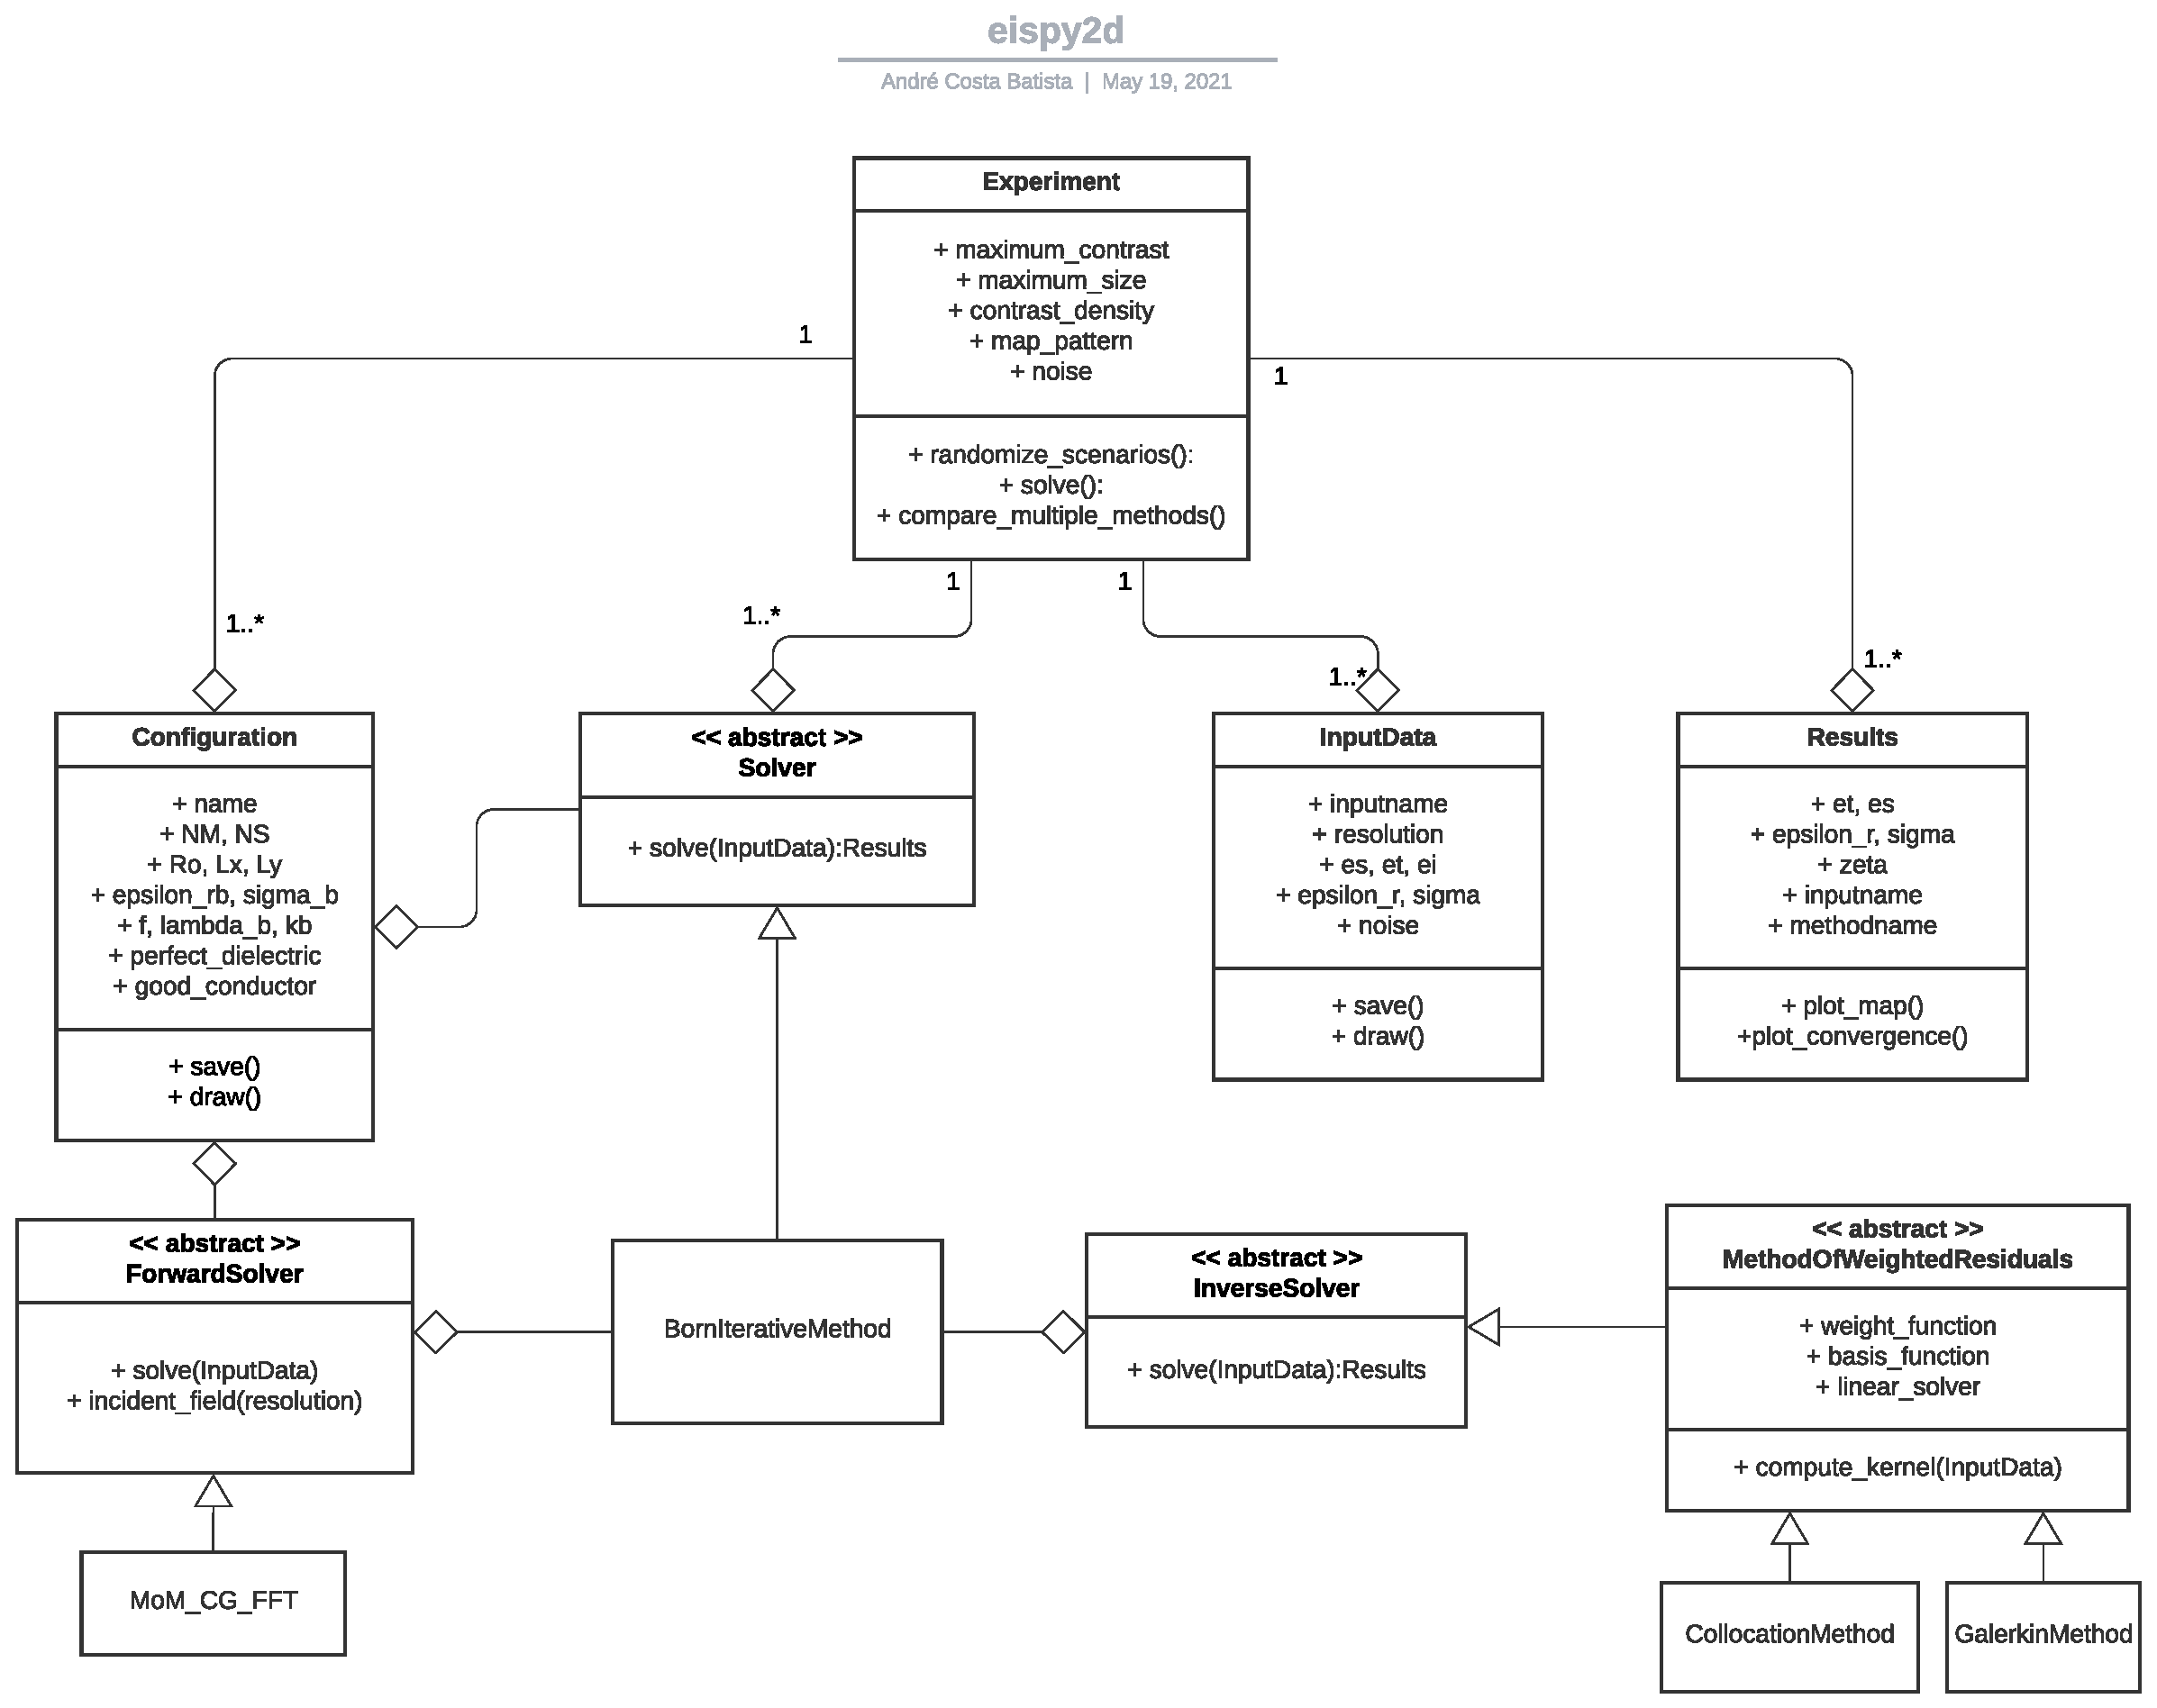
\includegraphics[width=.95\paperwidth, angle=90]{./figuras/eispy2d.eps}
			%	\vspace*{0.2in}
			%	\caption{UML Class Diagram of \textit{eispy2d} library.}
			%	\label{fig:4:eispy2d}
			%\end{figure}
			\begin{figure}[!h]
				\centering
				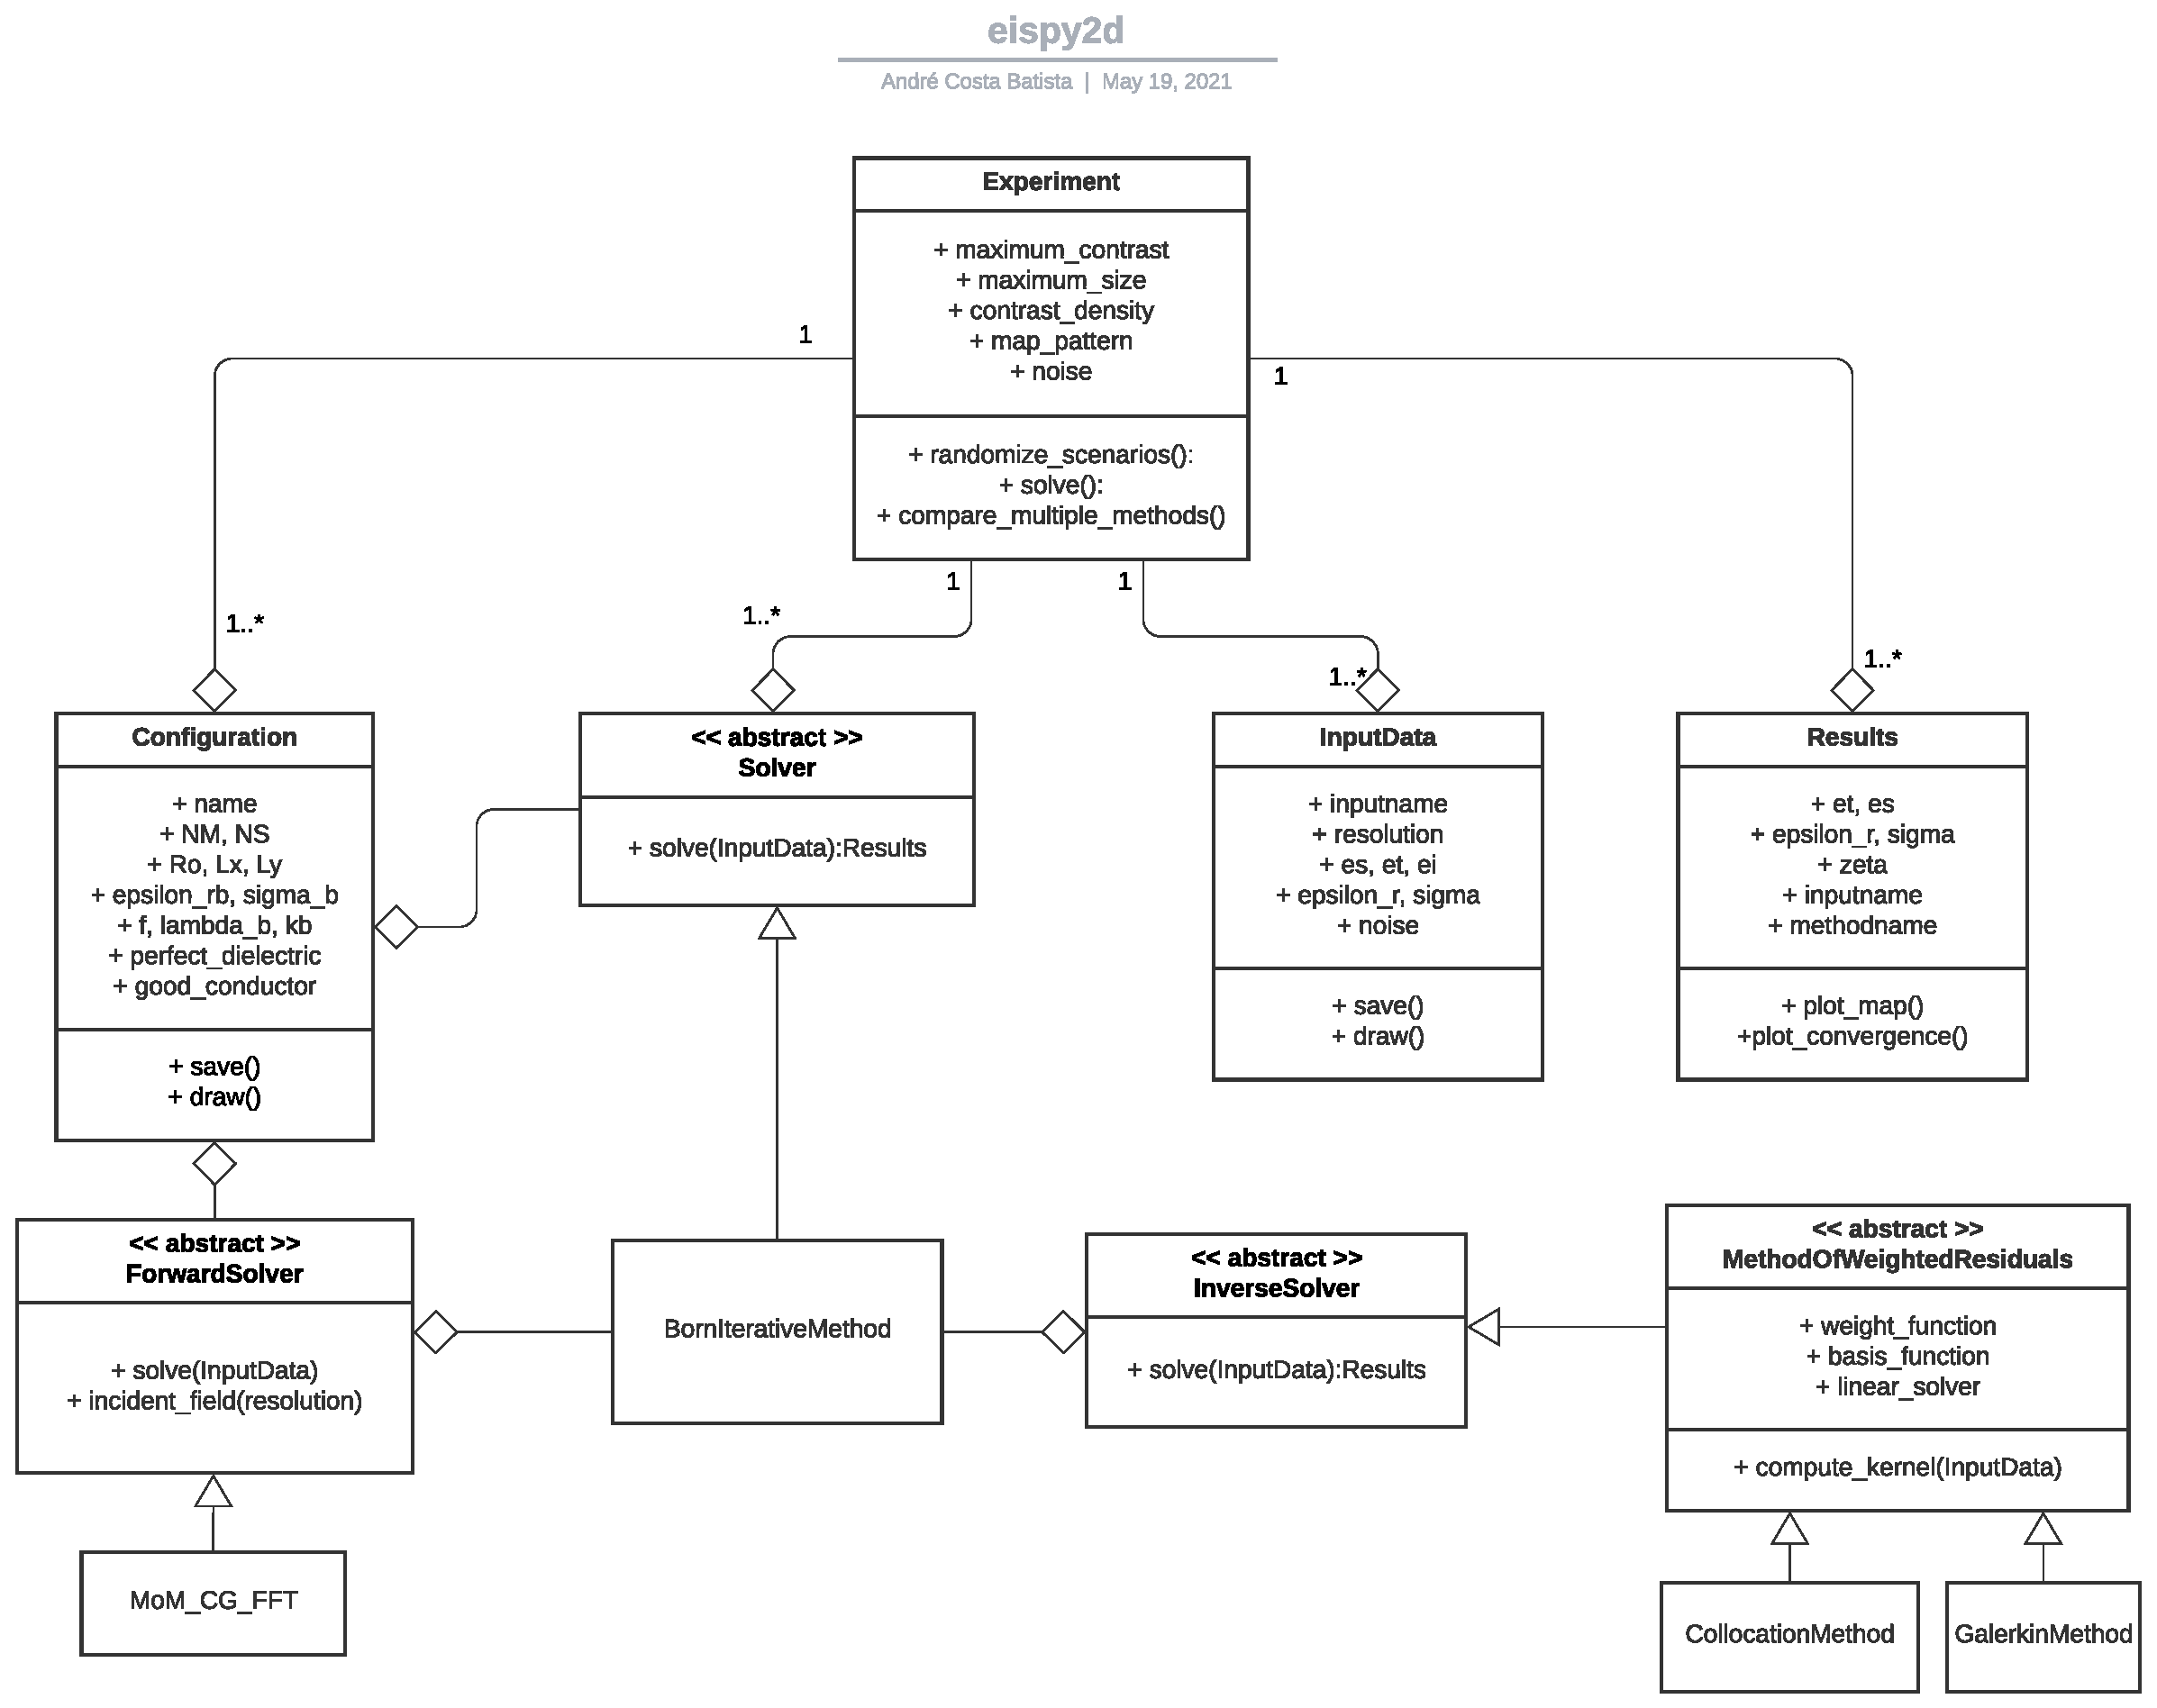
\includegraphics[width=\textwidth]{./figuras/eispy2d.eps}
				\caption[UML Class Diagram of \textit{eispy2d} library.]{UML Class Diagram of \textit{eispy2d} library.}
				\label{fig:4:eispy2d}
			\end{figure}
			
			%A seguir, uma breve explicação das classes principais:
			The following is a brief explanation of the main classes:
			\begin{enumerate}
				%\item\textbf{Configuration}: classe que guarda as informações principais do problema, como tamanho da imagem ($L_X$, $L_Y$), raio de observação ($R_O$), número de medições e de incidências ($N_M$, $N_S$);
				\item\textbf{Configuration}: a class that stores the primary information of the problem, such as image size ($L_X$, $L_Y$), observation radius ($R_O$), number of measurements and incidences ($N_M$, $N_S$);
				%\item\textbf{InputData}: classe que caracteriza uma instância de problema. Sua informação principal são os dados do campo espalhado. No entanto pode agregar outras informações como o campo total (para o problema linear) ou as imagens de contraste (para medição do erro);
				\item\textbf{InputData}: a class that characterizes a problem instance. Its primary information is the data of the scattered field. However, other information can be added, such as the total field (for the linear problem) or the contrast images (for error measurement);
				%\item\textbf{Results}: classe que guarda e exibe os resultados de uma execução do problema inverso não-linear. Além disso, também implementa os indicadores de qualidade;
				\item\textbf{Results}: a class that stores and displays the results of an execution of the nonlinear inverse problem. In addition, it also implements quality indicators;
				%\item\textbf{Solver}: uma classe abstrata para implementação de resolvedores do problema não-linear. Uma derivação, por exemplo, é a classe \textit{BornIterativeMethod} que implementa o correspondente método;
				\item\textbf{InverseSolver}: a abstract class for nonlinear inverse solvers implementation. For instance, inversion approaches such as the Born Iterative Method and the Subspace Optimization methods are derived classes which implement the corresponding methods.
				%\item\textbf{ForwardSolver}: classe abstrata para implementação de resolvedores diretos. Uma derivação, por exemplo, é o Método dos Momentos (\textit{MoM\_CG\_FFT});
				\item\textbf{ForwardSolver}: abstract class for implementing forward solvers. One derivation, for example, is the Method of Moments Conjugated Gradient-Fast Fourier Transform \citep{su1987calculation};
				%\item\textbf{InverseSolver}: classe abstrata para resolver o problema inverso linear. A classe \textit{MethodOfWeightedResiduals} é uma derivação ainda abstrata que serve para representar as discretizações \textit{CollocationMethod} e \textit{GalerkinMethod} e executar regularizadores como o de Tikhonov, Landweber e CG;
				\item\textbf{Discretization}: abstract class for discretization schemes. Each discretization strategy is a derived class, such as the Collocation Method (Subsection \ref{chap:methods:discretization:collocation}).
				%The \textit{MethodOfWeightedResiduals} class is a still abstract derivation that serves to represent the \textit{CollocationMethod} and \textit{GalerkinMethod} discretizations and execute regularizers such as Tikhonov, Landweber, and CG;
				%\item\textbf{Experiment}: classe que representa um experimento. É responsável por criar um conjunto de testes sintéticos aleatórios, executar os algoritmos e comparar resultados. Seus atributos principais são os parâmetros que configuram o conjunto de teste, i.e., o padrão de espalhado (geometrias tradicionais, aleatórias ou superfícies), o contraste máximo permitido, o tamanho máximo dos objetos, a densidade de contraste na imagem (quantidade de objetos na figura), entre outros.
				\item\textbf{Experiment}: an abstract class that represents an experiment. Two schemes are possible: case study and benchmark. For each corresponding class, there are appropriate methods for visualizing and comparing the results.
				\item\textbf{TestSet}: it is a class that contains a set of problem instances. There are appropriate methods for generating synthetic tests controlling multiple scatterer characteristics.
				% It is responsible for creating a set of random synthetic tests, executing the algorithms, plotting results, and comparing results. Its main attributes are the parameters that configure the test set, i.e., the scatter pattern (traditional, random, or surface geometries), the maximum allowed contrast, the maximum size of the objects, the density of contrast in the image (number of objects in the image), among others.
			\end{enumerate}

			%Para avaliar ou comparar a performance entre os algoritmos, três aspectos são fundamentais: os indicadores de qualidade, os princípios para criação de conjuntos de teste aleatórios e a metodologia de comparação. As próximas subsubseções trarão maiores explicações destes três aspectos. Cada um deles incluem tanto técnicas já conhecidas quanto novas propostas implementadas neste trabalho que a contribuição desta investigação é uma estrutura mais robusta de experimentação sintética.
			Three aspects are fundamental to evaluate or compare the performance among the algorithms: the quality indicators, the principles for creating random test sets, and the comparison methodology. The following subsections will provide further explanations of these three aspects. Each of them includes both techniques already known and newly proposed ones; therefore, this investigation's contribution is a more robust structure of synthetic experimentation.
			
		\subsection{Performance Metrics Proposal}\label{chap:proposed-methodology:library:metrics}
		
			%Um conjunto de indicadores foram implementados para a avaliar a qualidade da reconstrução feita pelos algoritmos. De maneira similar a \eqref{eq:4:error0:epsilon}, o erro percentual médio de estimação da permissividade relativa e o erro médio de estimação da condutividade serão calculados por:
			A set of indicators were implemented to assess the quality of the reconstruction done by the algorithms. The indicator were chosen according to their popularity throughout the references in the literature. The intention is also to aggregate indicators with different to enable multiple ways to analyze the performance of a method. Similar to \eqref{eq:4:error0:epsilon}, the average percentage error of estimation of relative permittivity and the average error of estimation of conductivity will be calculated by:
			\begin{align}
				\zeta_{\epsilon PAD} &= \frac{1}{N_IN_J}\sum\limits_{i=1}^{N_I}\sum\limits_{j=1}^{N_J}\left|\frac{\epsilon^*_{r,ij}-\epsilon_{r,ij}}{\epsilon^*_{r,ij}}\right|\times100~[\%/\mathrm{pixel}] \label{eq:4:zeta:epad} \\
				\zeta_{\sigma AD} &= \frac{1}{N_IN_J}\sum\limits_{i=1}^{N_I}\sum\limits_{j=1}^{N_J}\left|\sigma^*_{ij}-\sigma_{ij}\right|~[\mathrm{S}/\mathrm{pixel}] \label{eq:4:zeta:sad}
			\end{align}
			
			%Além disso, foram implementados métricas similares a \eqref{eq:4:zeta:epad} e \eqref{eq:4:zeta:sad} mas que atuam particularmente sobre as regiões de fundo e de objeto. São eles:
			In addition, metrics similar to \eqref{eq:4:zeta:epad} and \eqref{eq:4:zeta:sad} were implemented, considering background and object regions only. They are:
			\begin{align}
				\zeta_{\epsilon BE} &= \frac{1}{N_B}\sum\limits_{\epsilon^*_{r,ij}=\epsilon_{rb}}^{N_I,NJ}\left|\frac{\epsilon^*_{r,ij}-\epsilon_{r,ij}}{\epsilon^*_{r,ij}}\right|\times100~[\%/\mathrm{pixel}] \label{eq:4:zeta:ebe} \\
				\zeta_{\sigma BE} &= \frac{1}{N_B}\sum\limits_{\sigma^*_{ij}=\sigma_{b}}^{N_I,NJ}\left|\sigma^*_{ij}-\sigma_{ij}\right|~[\mathrm{S}/\mathrm{pixel}] \label{eq:4:zeta:sbe} \\
				\zeta_{\epsilon OE} &= \frac{1}{N_O}\sum\limits_{\epsilon^*_{r,ij}\neq\epsilon_{rb}}^{N_I,NJ}\left|\frac{\epsilon^*_{r,ij}-\epsilon_{r,ij}}{\epsilon^*_{r,ij}}\right|\times100~[\%/\mathrm{pixel}] \label{eq:4:zeta:eoe} \\
				\zeta_{\sigma OE} &= \frac{1}{N_O}\sum\limits_{\sigma^*_{ij}\neq\sigma_{b}}^{N_I,NJ}\left|\sigma^*_{ij}-\sigma_{ij}\right|~[\mathrm{S}/\mathrm{pixel}] \label{eq:4:zeta:soe}
			\end{align}
			
			%\noindent onde $N_B$ e $N_O$ são o número elementos de fundo e de objeto, respectivamente. O objetivo dessas métricas é medir especificamente a capacidade de estimar o contraste de um objeto e de evitar perturbações nas regiões de fundo.
			\noindent where $N_B$ e $N_O$ are the numbers of background and object elements, respectively. The purpose of these metrics is to precisely measure the ability to estimate the contrast of an object and avoid perturbations in the background regions.
			
			%Em relação a EAs que otimizam simultâneamente contraste e campo, pode ser muito interessante medir a capacidade de estimar o campo total na região da imagem. Por isso, foram implementados os seguintes indicadores:
			Concerning EAs that simultaneously optimize contrast and field, measuring the ability to estimate the total field in the image region is a potential tool. For this reason, the following indicators were implemented:
			\begin{align}
				\zeta_{TFMPAD} &= \frac{1}{N_PN_QN_R}\sum\limits_{p=1}^{N_P}\sum\limits_{q=1}^{N_Q}\sum\limits_{r=1}^{N_R}\left|\frac{|E^*_{pqs}|-|E_{pqs}|}{|E^*_{pqs}|}\right|\times100~[\%/\mathrm{pixel}] \label{eq:4:zeta:tfmpad} \\
				\zeta_{TFPAD} &= \frac{1}{N_PN_QN_R}\sum\limits_{p=1}^{N_P}\sum\limits_{q=1}^{N_Q}\sum\limits_{r=1}^{N_R}\left|\measuredangle E^*_{pqs} - \measuredangle E_{pqs}\right| ~[\mathrm{rad}/\mathrm{pixel}] \label{eq:4:zeta:tfpad}
			\end{align}
			
			%\noindent onde o operador ``$\measuredangle$'' representa a fase do número complexo. Portanto, esses dois indicam medem o erro médio de magnitude e fase da estimativa do campo elétrico.
			\noindent where the operator ``$\measuredangle$'' represents the phase of the complex number. Therefore, these two indicators measure the average magnitude and phase error of the electric field estimate.
			
			%Quando um algoritmo erra na localização e na detecção da forma dos objetos, as métricas \eqref{eq:4:zeta:epad}-\eqref{eq:4:zeta:soe} serão afetadas. No entanto, pode ser que um algoritmo estime bem a forma e o contraste de um objeto mas, por erros na posição, a avaliação dessa solução pelas métricas seja baixa. Para levar em conta especificamente a capacidade de detectar posição e forma, são propostas duas métricas.
			When an algorithm fails to locate and detect the shape of objects, metrics \eqref{eq:4:zeta:epad}-\eqref{eq:4:zeta:soe} will be affected. However, it may be that an algorithm estimates the shape and contrast of an object well, but due to errors in position, the evaluation of this solution by the metrics is low. Two metrics are proposed to take specific account of the ability to detect position and shape.
			
			%Para avaliar a capacidade de estimar a posição de objetos, é proposto um indicador baseado na distância entre os ``centros de massa'' dos objetos nas imagens:
			An indicator based on the distance between the ``centers of mass'' of the objects in the images is proposed to assess the ability to estimate the position of objects:
			\begin{equation}
				\zeta_P  = \sqrt{(x^*_c-x_c)^2 + (y^*_c-y_c)^2}\times 100~[\%] \label{eq:4:zeta:p}
			\end{equation}
			
			%\noindent onde ($x^*_c$, $y^*_c$) é centro da figura original e ($x_c$, $y_c$) é o centro da imagem reconstruída. Os centros são calculados conforme \autoref{alg:zetap}. Após a limiarização da imagem reconstruída, os valores de contraste são descartados. Isto é feito para evitar que erros na estimativa do contraste influenciem na ponderação do centro. Desta forma, esse indicador pode ser utilizado tanto para imagens com objetos únicos como múltiplos.
			\noindent where ($x^*_c$, $y^*_c$) is the center of the original figure and ($x_c$, $y_c$) is the center of the reconstructed image. The centers are calculated according to Algorithm \ref{alg:zetap}. After the threshold of the reconstructed image, the contrast values are discarded. This is done to prevent errors in the contrast estimation from influencing the center weighting. In this way, this indicator can be used for images with single or multiple objects.
			\begin{algorithm}[!htb]
				\caption{$\zeta_P$ measure.}
				\label{alg:zetap}
				\KwIn{$\boldsymbol{\chi^{*}}$, $\boldsymbol{\chi}$}
				\KwOut{$\zeta_P$}
				$\chi_{thres} \leftarrow \min\{|\boldsymbol{\chi}|\} + \frac{1}{2}\left(\max\{|\boldsymbol{\chi}|\}-\min\{|\boldsymbol{\chi}|\}\right)$\\
				$\chi^{*}_{ij}\leftarrow1~\forall\chi^{*}_{ij}\neq0$\\
				$\chi_{ij}\leftarrow\begin{cases} 0, &\forall\chi_{ij}<\chi_{thres} \\ 1, &\forall\chi_{ij}\ge\chi_{thres}\end{cases}$ \\
				$x_i \leftarrow (i-1)/(N_I-1) \forall i = 1, \cdots, N_I$\\
				$y_j \leftarrow (j-1)/(N_J-1) \forall j = 1, \cdots, N_J$\\
				$x^*_c\leftarrow \frac{\sum_{i=1}^{N_I}\sum_{j=1}^{N_J} x_i\chi^*_{ij}}{\sum_{i=1}^{N_I}\sum_{j=1}^{N_J}\chi^*_{ij}}$ \\
				$y^*_c\leftarrow \frac{\sum_{i=1}^{N_I}\sum_{j=1}^{N_J} y_j\chi^*_{ij}}{\sum_{i=1}^{N_I}\sum_{j=1}^{N_J}\chi^*_{ij}}$ \\
				$x_c\leftarrow \frac{\sum_{i=1}^{N_I}\sum_{j=1}^{N_J} x_i\chi_{ij}}{\sum_{i=1}^{N_I}\sum_{j=1}^{N_J}\chi_{ij}}$ \\
				$y_c\leftarrow \frac{\sum_{i=1}^{N_I}\sum_{j=1}^{N_J} y_j\chi_{ij}}{\sum_{i=1}^{N_I}\sum_{j=1}^{N_J}\chi_{ij}}$ \\
				$\zeta_P  = \sqrt{(x^*_c-x_c)^2 + (y^*_c-y_c)^2}\times 100~[\%]$
			\end{algorithm}
			
			%Para avaliar a capacidade de reconstruir a forma dos objetos, foi necessário utilizar um algoritmo de detecção de contornos nas imagens. O algoritmo Marching Cubes \citep{lorensen1987marching} é uma técnica clássica de identificação de contornos em imagens tridimensionais. A biblioteca \textit{scikit-image} possui uma implementação eficiente do caso dimensional que será utilizada nesse trabalho \citep{walt2014scikit}. A partir disso, a métrica de forma $\zeta_S$ é definida em termos da razão entre a área da diferença entre os contornos das duas imagens e a área da imagem original. A implementação e um exemplo para o cálculo desta métrica pode ser visualizada no Anexo \ref{annex:zetas}. Tanto $\zeta_S$ quanto $\zeta_P$ são indicadores que não existem ainda na literatura e estão sendo propostas nesse trabalho. Também não foi visto na literatura indicadores como $\zeta_{TFMPAD}$ e $\zeta_{TFPAD}$. Embora eles não tenham tanta relevância por não ser o objetivo principal reconstruir o campo, eles podem auxiliar no entendimento do desempenho dos métodos, principalmente dos estocásticos que otimizam simultâneamente contraste e campo.
			It was necessary to use an algorithm for detecting contours in the images to assess the ability to reconstruct the shape of the objects. The Marching Cubes algorithm \citep{lorensen1987marching} is a classic technique for identifying contours in three-dimensional images. The \textit{scikit-image} library efficiently implements the two-dimensional case, which is considered in this work \citep{walt2014scikit}. Then, the shape metric $\zeta_S$ is defined in terms of the ratio between two areas: (i) the area of the difference between the contours of the two images; and (ii) the area of the original image. The implementation and an example for calculating this metric can be seen in Appendix \ref{annex:zetas}. This approach is not as sophisticated as the one proposed by \cite{kurrant2021evaluating}, since the former is based on a threshold technique while the latter is based on image segmentation through a machine learning technique, which is more robust. In addition, their diverse set of metrics for breast reconstruction can also be adapted to our general scheme and it will be consider in the future. However, up to the date of this thesis, both $\zeta_S$ and $\zeta_{P}$ are indicators that have not been addressed in the literature. Also, indicators such as $\zeta_{TFMPAD}$ and $\zeta_{TFPAD}$ were not seen in the literature. Although they are not so relevant since it is not the primary objective to reconstruct the field, they can help understand the performance of some methods, especially the stochastic ones that simultaneously optimize contrast and field.
		
		\subsection{Randomization of the Test Set}\label{chap:proposed-methodology:library:randomization}
		
			%Em muitos trabalhos, os experimentos sintéticos são planejados para demonstrar a capacidade de reconstrução dos algoritmos em cenários variados. Tradicionalmente, geometrias comuns são utilizadas para explorar situações como presença de espalhadores fortes, diferentes níveis de ruído, separação de objetos, heterogeneidades, entre outros. Normalmente, as imagens utilizadas nos testes são definidas arbitrariamente e a performance em tipo de situação é estudada com apenas um ou poucos exemplos de imagens.
			In many studies, synthetic experiments are designed to demonstrate the ability to reconstruct the algorithms in different scenarios. Traditionally, common geometries are used to explore situations such as strong scatterers, different noise levels, separation of objects, heterogeneities, among others. Usually, the images used in the tests are defined arbitrarily, and the performance in the corresponding situation is studied with only one or a few examples of images.
			
			%Para dar alguns exemplos, citaremos alguns trabalhos recentes e relevantes na literatura: (i) \cite{zhong2020multiresolution} utilizaram um tipo de imagem pra fazer comparações entre quatro níveis de ruído e um tipo de imagem para compara situação de alto contraste; (ii) \cite{wei2019deep} usam quatro imagens para cada um dos dois níveis de contraste e três imagens para estudar a reconstrução de objetos condutivos; e (iii) \cite{salucci2017multifrequency} usou uma imagem para testes sem ruído, uma imagem para dois níveis de ruído, uma imagem para não-homogeneidade e uma imagem para alto contraste. Nestes trabalhos, vale destacar que as imagens ou são compostas por somente círculos ou único quadrado ou o tradicional perfil Austria (composto por um anel e dois círculos). No entanto, vale destacar também que, em \citep{wei2019deep}, os autores utilizaram seis imagens de uma base formada por handwritng digits comumente usada em Machine Learning; em \citep{shah2018fast} e \citep{batista2021quadratic}, os autores usam quatro imagens com geometrias diferentes para experimentos com objetos únicos e três para não-homogeneidades com diferentes geometrias.
			To give some examples, some recent and relevant works in the literature are mentioned: (i) \cite{zhong2020multiresolution} used an image type to make comparisons between four noise levels and an image type to compare high contrast situations; (ii) \cite{wei2019deep} use four images for each of the two levels of contrast and three images to study the reconstruction of conductive objects; and (iii) \cite{salucci2017multifrequency} used an image for tests without noise, an image for two levels of noise, an image for inhomogeneity and an image for high contrast. In these works, it is worth mentioning that the images are either composed of only circles or a single square or the traditional Austria profile (composed of a ring and two circles). However, it is also worth noting that, in \citep{wei2019deep}, the authors used six images of a base formed by handwritng digits commonly used in Machine Learning; in \citep{shah2018fast} and \citep{batista2021quadratic}, the authors use four images with different geometries for experiments with single objects and three for inhomogeneities with different geometries.
			
			%De fato, o estilo de experimentação que é tradicionalmente usado exemplifica a capacidade do algoritmo de lidar com diferentes situações e isso é relevante para a testagem do método. No entanto, não seria mais robusto avaliar a performance com experimentos sintéticos através um conjunto suficientemente grande de imagens com geometrias aleatórias? Não seria esse um procedimento mais robusto para estudar a performance média dos algoritmos? A performance média em conjuntos de teste aleatórios não seria melhor do que o estudo com imagens arbitrárias para fazer uma comparação mais eficiente? Esse tipo de estudo não seria relevante para a literatura tal como já é na área de comparação de algoritmos de otimização \citep{beiranvand2017best}?
			In fact, the form of experimentation traditionally used exemplifies the algorithm's ability to deal with different situations, which is relevant for testing the method. A more robust approach to evaluating algorithmic performance would be to utilize synthetic experiments on a sufficiently large dataset of images with randomized geometries. Such a methodology can provide a more comprehensive understanding of the average performance of the algorithms. The utilization of random test sets to assess average performance is more effective than using arbitrary images to make a more efficient comparison. Conducting such studies may be of significant value to the existing literature on optimization algorithms \citep{beiranvand2017best}. % However, would it not be more robust to evaluate performance with synthetic experiments through a sufficiently large set of images with random geometries? Would this not be a more robust procedure to study the average performance of the algorithms? Would the average performance in random test sets not be better than the study with arbitrary images to make a more efficient comparison? Would this type of study not be relevant to the literature as it is already in the comparison of optimization algorithms \citep{beiranvand2017best}?
			
			%Para explorar esse tipo de experimentação, foi desenvolvido um processo de geração de conjunto de testes aleatórios dentro da classe \textit{Experiment} na biblioteca \textit{eispy2d}. Um conjunto de testes é gerado conforme os seguintes parâmetros de configuração:
			A process of generating a set of random tests was developed to explore this experimentation design. It is embedded within the \textit{TestSet} class in the \textit{eispy2d} library. A set of tests is generated according to the following configuration parameters:
			\begin{itemize}
				%\item Padrão de geometrias: esse parâmetro significa que tipo de geometrias serão consideradas. Três padrões foram implementados: geometrias regulares\footnote{Quadrado, retângulo, triângulo equilátero, cruz, círculo, anel, elipse, losângulo, trapézio, paralelograma, polígonos de mais 5 lados (pentágono, hexágono etc) e estrelas de 4, 5 e 6 pontas.}, polígonos aleatórios\footnote{Polígonos de 3 lados ou mais com raio entre centro e vérticos aleatórios.} e superfícies aleatórias\footnote{Somatório de senos ou exponenciais}.
				\item Geometry pattern: this parameter means what type of geometries will be considered. Three patterns were implemented: regular geometries\footnote{Square, rectangle, equilateral triangle, cross, circle, ring, ellipse, rhombus, trapezoid, parallelogram, polygons of more than five sides (pentagon, hexagon, etc.) and stars of 4, 5, and 6 points.}, random polygons\footnote{Polygons of 3 sides or more with random radius between the center and vertices.}, and random surfaces\footnote{Sum of sines or exponentials.}.
				%\item Máximo contraste: esse parâmetro controla o intervalo de contraste permitido para os objetos inseridos na imagem. Também é possível configurar esse parâmetro para que todos os objetos sejam definidos com esse contraste. Ou seja, o conjunto de testes pode ser criado tanto para estudar o desempenho com diferentes contrastes quanto únicos.
				\item Maximum contrast: this parameter controls the allowed contrast range for the objects inserted in the image. It is also possible to configure this parameter so that all objects are defined with this contrast. In other words, the set of tests can be created both to study performance with different and unique contrasts.
				%\item Máximo tamanho: esse parâmetro regula o tamanho dos objetos. Também pode ser definido como valor máximo ou configurado para valor fixo. No caso de geometrias regulares, todas elas são configuradas para que o raio entre o centro e o vértice mais afastado seja definido por esse parâmetro. Em outras palavras, é o maior desenho da geometria que cabe dentro de um círculo definido por esse parâmetro. No caso de polígonos aleatórios, esse parâmetro regula o raio máximo que cada vértice pode ter. No caso de exponenciais, esse parâmetro regula o raio máximo do centro da exponencial até três vezes o desvio padrão.
				\item Maximum size: this parameter regulates the size of objects. It can also be set to a maximum value or assigned to a fixed value. In regular geometries, all of them are configured so that this parameter defines the radius between the center and the furthest vertex. In other words, it is the largest geometry drawing that fits within a circle defined by this parameter. In the case of random polygons, this parameter regulates the maximum radius that each vertex can have. In exponentials, this parameter controls the maximum radius of the exponential up to three times the standard deviation. % (see Appendix \ref{annex:geometries} for more information)
				%\item Máxima densidade de contraste: regula o valor máximo da média de contraste por píxel da imagem. Esse parâmetro regula a quantidade de objetos na imagem.
				\item Maximum contrast density: regulates the maximum value of the average contrast per pixel of the image. This parameter regulates the number of objects in the image.
				%\item Ruído: nível de ruído no qual os dados do campo espalhado vão ser corrompidos.
				\item Noise: noise level at which the data in the scattered field will be corrupted.
				%\item Tamanho amostral: quantidade de imagens de teste no conjunto.
				\item Sample size: number of test images in the set.
			\end{itemize}
			%É importante destacar que cada geometria inserida em uma imagem tem rotação e posição definidas aleatoriamente. Portanto, o objetivo deste processo é criar benchmarks que possibilitem o estudo da performance do métodos sejam em configurações isoladas mas também na evolução de efeitos (e.g., a evolução da performance no crescimento do contraste). Não somente isso, esse processo permite estudar fatores de efeito na performance dos algoritmos para o problema isolando o viés presente na escolha arbitrária das geometrias. Essa implementação considera apenas experimentos sintéticos. No entanto, esses princípios poderiam ser utilizados para um projeto de um benchmark real, i.e., medições reais de espalhamentos os quais são definidos seguindo esses princípios de aleatorização de geometrias e isolamente de fatores de efeito.
			It is important to highlight that each geometry inserted in an image has a randomly defined rotation and position. Therefore, this process aims to create benchmarks that make it possible to study the performance of the methods in isolated configurations and the evolution of effects (e.g., the progression of performance in the growth of the contrast). Moreover, this process allows the study of effect factors on the performance of the algorithms for the problem, isolating the bias present in the arbitrary choice of geometries. This implementation considers only synthetic experiments. However, these principles could be used for a project of a real benchmark, i.e., physical measurements, which are defined following these principles of randomization of geometries and in isolation of effect factors.
		
		\subsection{Comparison Structure}\label{chap:proposed-methodology:library:comparison}
		
			%Quando um método é executado para um conjunto de testes, o indicador de performance é calculado para solução final de cada instância do conjunto. A informação dos resultados pode ser visualizada de diferentes formas. Duas das formais mais tradicionais para visualizar os dados de uma amostra é o \textit{boxplot} e o \textit{violinplot} \citep{chen2008handbook}. A primeira é importante para visualizar os quantis de uma amostra e a última é importante para ter uma noção da distribuição dos dados. Rotinas para visualização dos dados dos experimentos através desses dois gráficos foram implementadas a partir da biblioteca \textit{matplotlib} \citep{hunter2007matplotlib}. Além disso, as rotinas também implementam a visualização de mais de um conjunto de teste em um mesmo gráfico o qual é relevante para visualizar a evolução da performance de um método quando se varia algum parâmetro na configuração dos testes (e.g., contraste máximo). Também foi utilizado o gráfico Quantile-Quantile para verificação de premissas de normalidade de distribuição implementados pela rotina \textit{qqplot} da biblioteca \textit{pingouin} \citep{vallat2018pingouin}.
			When a method runs a set of tests, the performance indicator is calculated for the final solution of each instance. The results information can be viewed in different ways. Two of the most traditional ways to visualize the data of a sample are the \textit{boxplot} and the \textit{violinplot} \citep{chen2008handbook}. The first is essential to visualize the quartiles of a sample, and the last is important to get a sense of the distribution of the data. Routines for visualizing the data of the experiments through these two graphs were implemented from the \textit{matplotlib} library \citep{hunter2007matplotlib}. In addition, the routines also implement the visualization of more than one test set in the same graph, which is relevant to visualize the evolution of the performance of a method when a parameter in the test configuration varies (e.g., maximum contrast). The Quantile-Quantile graph was also used to verify assumptions of normality distribution implemented by the \textit{qqplot} routine of the \textit{pingouin} library \citep{vallat2018pingouin}.
			
			%Os conjuntos de teste representam uma amostra de um universo de casos possíveis. A informação da performance média de método em um universo particular pode ser relevante tanto para cumprir especificações numa dada aplicação quanto para comparação com outras metodologias. Como esse universo de casos é muito grando, se não infinito, é muito comum estimar o intervalo de confiança dessa média, i.e., uma faixa de valores que têm uma alta probabilidade de conter a média verdadeira. Este tipo de estudo é feito utilizando ferramentas estatísticas que possibilitam não somente estimar a média como também comparar outras, ou seja, fazer comparações entre performances médias de algoritmos ou conjuntos de teste. Não está no escopo desta dissertação uma explicação sobre os métodos estatísticos que foram utilizados. Para uma melhor compreensão, recomendamos a leitura de \citep{montgomery2010applied} e as implementações da biblioteca \textit{statsmodels} \citep{seabold2010statsmodels}. Neste texto será somente apresentado o processo de comparação entre duas e múltiplas amostras as quais representam os resultados de um indicador para diferentes métodos em um mesmo conjunto de testes.
			The test sets represent a sample of a universe of possible cases. The information on the average performance of the method in a particular universe can be relevant to comply with specifications in a given application and for comparison with other methodologies. As this universe of cases is very large, if not infinite, it is common to estimate the confidence interval of this average. The confidence interval can be understood as the range in which, if we repeat the experiment many times, the sampled average will be within that range in a specified percentage of the number of times. This type of study is done using statistical tools that make it possible to estimate the average and compare others, that is, to make comparisons between average performances of algorithms or test sets. It is not in the scope of this dissertation to explain the statistical methods that were used. Reading \citep{montgomery2010applied} and the implementations of the \textit{statsmodels} library \citep{seabold2010statsmodels} are recommend for a better understanding. In this text, only the comparison process between two and multiple samples will be presented, representing the results of an indicator for different methods in the same set of tests.
			
			%Para comparações entre dois métodos estocásticos em um mesmo teste, o seguinte processo foi implementado:
			For a comparison between two stochastic methods in a same test instance, the following process was implemented:
			\begin{enumerate}
				\item If the Shapiro-Wilk test does not show a deviation from normality for both samples, then the Two Sample T-Test with a significance of 5\% is performed. The effect size\footnote{The effect size, in this case, means the minimum difference for which it is possible to identify a false-negative error for the desired power and sample size, i.e., when the hypothesis of equality is not rejected when it is false.} is calculated for a power of 80\%. If a difference is detected, then there is evidence for the superiority of one of the methods.
				\item If the Shapiro-Wilk test shows a deviation from the normal distribution for any of the samples, then the test is repeated using logarithmic and square-root transformations on the data. If a transformation is successful, the same transformation is applied for the other sample, the same procedure as the previous step is repeated, and the same conclusions can be drawn.
				\item If none of the transformations are successful, then the Mann–Whitney U test is performed, which allows detecting whether, when randomly selecting an element from each sample, the probability that one element is greater than the other is not the same as otherwise. If the difference is detected at a significance level of 5\%, then there is evidence for the superiority of one of the methods.
			\end{enumerate}
		
			When considering the a stochastic method and a deterministic one, then a similar procedure is employed. When the distribution of the results from the stochastic method is approximately normal, then an One-Sample T-Test is performed. When data transformation is necessary, then the transformation is also applied to the result of the deterministic method. When the distribution of the results obtained by the stochastic method is not normal, approximately, then the Wilcoxon Signed-Rank Test is performed. The test is able to detect whether stochastic data comes from a symmetric population with a specified median which, in this case, is the result obtained by the deterministic method.
			
			%O processo de comparação da perfomance de um indicador entre dois métodos em para um mesmo conjunto de teste foi implementado segundo uma lógica pareada. Uma vez que se trata dos resultados dos métodos para um mesmo conjunto de teste, a média estimada é definida em termos da diferença entre indicadores dos dois métodos em cada instância. O processo pode ser resumido da seguinte forma:
			The process of comparing the performance of an indicator between two methods in the same test set was implemented according to a paired fashion. Through the results of the methods for the same test set, the estimated average is defined in terms of the difference between indicators of the two methods in each instance.  The process can be summarized as follows:
			\begin{enumerate}
				%\item Se o teste de Shapiro-Wilk não acusar um desvio da normalidade sobre a diferença pareada, então o Teste T-Pareado com significância de 5\% é realizado e o tamanho de efeito\footnote{O tamanho de efeito neste caso significa a diferença mínima pareada para o qual é possível indentificar um erro de falso-negativo para a potência desejada e tamanho amostral, i.e., quando a hipótese de iguadade não é reijeitada quando é falsa.} é calculado para uma potência de 80\%. Se for detectada uma diferença, então haverá evidência para a superioridade de um dos métodos.
				\item If the Shapiro-Wilk test does not show a deviation from normality over the paired difference, then the Paired T-Test with a significance of 5\% is performed. The effect size is calculated for a power of 80\%. If a difference is detected, then there is evidence for the superiority of one of the methods. % \footnote{The effect size, in this case, means the minimum paired difference for which it is possible to identify a false-negative error for the desired power and sample size, i.e., when the hypothesis of equality is not rejected when it is false.}
				%\item Se o teste de Shapiro-Wilk acusar um desvio da normalidada sobre a diferença pareada, então o teste é repetido utilizando transformações logarítmicas e de raiz quadrada sobre os dados. Se uma transformação tiver sucesso, então o mesmo procedimento do passo anterior é repetido e as mesmas conclusões podem ser obtidas.
				\item If the Shapiro-Wilk test shows a deviation from the normal distribution over the paired difference, then the test is repeated using logarithmic and square-root transformations on the data. If a transformation is successful, then the same procedure as the previous step is repeated, and the same conclusions can be drawn.
				%\item Se nenhuma das transformações tiver sucesso, então é realizado o Teste de Wilcoxon que permite detectar as diferenças seguem uma distribuição simétrica ao redor de zero. Se a diferença for detectada a um nível de significância de 5\%, então haverá evidência para a superioridade de um dos métodos.
				\item If none of the transformations are successful, then the Wilcoxon Test is performed, which allows the detection of differences following a symmetrical distribution around zero. If the difference is detected at a significance level of 5\%, then there is evidence for the superiority of one of the methods.
			\end{enumerate}
			%As premissas de independência entre os dados são garantidas pelo fato da independência das execuções dos algoritmos. As rotinas utilizadas para o teste normal são as da biblioteca \textit{statsmodels} e a rotina do teste não-normal provém da biblioteca \textit{scipy} \citep{scipy}.
			The independence assumption between the data is guaranteed because the algorithms’ execution is independent. In other words, the pseudo-random variables used in each algorithm are generated with sufficient independence, establishing the independence of samples. When the normality assumption is valid, the routines used are those in the \textit{statsmodels} library, and the non-normal test routine comes from the \textit{scipy} library \citep{scipy}.
			
			%O processo de comparação entre múltiplos métodos se dá pela técnica de Análise de Variâncias (ANOVA) \citep{montgomery2010applied}. O processo de comparação se dá através da seguinte forma:
			The comparison process between multiple stochastic methods in the same test takes place using the analysis of variances (ANOVA) \citep{montgomery2010applied}. The comparison process is described as follows:
			\begin{enumerate}
				%\item Os resíduos de cada amostra em relação às suas médias amostrais são calculadas.
				\item The residues of observations and their corresponding sample means are evaluated.
				%\item Se o Teste de Shapiro-Wilk não acusar um desvio da distribuição dos resíduos, seja sem ou com transformações:
				\item If the Shapiro-Wilk test does not indicate a deviation between residuals and normal distributions, either with or without transformations:
				\begin{enumerate}
					%\item Se o Teste de Fligner não acusar invalidade da condição de homocedasticidade\footnote{A condição de homocedasticidade significa igualdade de variâncias das amostras.}, então o One Way ANOVA é executado sob o nível de significância de 5\%. O resultado indicará se existe evidência para pelo menos uma performance diferente das demais ou não. Também é calculado o tamanho de efeito para uma potência de 80\%.
					\item If the Fligner Test does not indicate invalidity of the homoscedasticity assumption\footnote{The homoscedasticity assumption means equal sample variances.}, then the One Way ANOVA is performed under the 5\% significance level. The result will indicate whether there is evidence for at least one performance different from the others or not. The effect size is also calculated for a power of 80\%.
					%\item Se o Teste de Fligner acusar invalidade da premissa de homocedasticidade, então é executado o teste Welch ANOVA o qual poderá indicar evidência para pelo menos uma performance diferente das demais sob um nível de significância de 5\%.
					\item If the Fligner test reveals invalidity of the homoscedasticity premise, then the Welch ANOVA test is performed, which may indicate evidence for at least one performance different from the others under a 5\% significance level.
					%\item Se for detectada alguma diferença e for necessário tentar identificar todas as possíveis superioridades de performance:
					\item If any differences are detected and it is necessary to try to identify all possible performance superiorities:
					\begin{enumerate}
						%\item Se a condição de homocedasticidade for válida, será realizado o Teste Tukey HSD de Comparações Múltiplas e serão detectadas todas as diferenças com a correção de significância necessária.
						\item If the homoscedasticity assumption is valid, the Tukey HSD Multiple Comparison Test will be performed and all differences will be detected with the necessary significance correction.
						%\item Se a condição de homocedasticidade não for válida, então as múltiplas comparações serão feitas a partir de múltiplos teste de Welch para amostras independentes com a significância determinada pela correção de Bon-Ferroni.
						\item If the homoscedasticity condition is not valid, multiple comparisons will be made from multiple Welch T tests for independent samples with the significance determined by the Bonferroni correction.
					\end{enumerate}
					%\item Se for detectada alguma diferença e for necessário identificar somente se um dos métodos é superior ou inferior aos outros:
					\item If a difference is detected and it is necessary to identify if all methods are superior or inferior to a single one (all versus one):
					\begin{enumerate}
						%\item Se a condição de homocedasticidade for válida, será realizado o Teste de Dunnet com a correção de significância necessária.
						\item If the homoscedasticity condition is valid, the Dunnet Test will be performed with the necessary significance correction.
						%\item Se a condição de homocedasticidade não for válida, então as comparações serão feitas a partir de teste de Welch para amostras independentes com a significância determinada pela correção de Bon-Ferroni.
						\item If the homoscedasticity premise is not valid, then the comparisons will be made using the Welch test for independent samples with the significance determined by the Bonferroni correction.
					\end{enumerate}
				\end{enumerate}
				%\item Se não for possível assumir a normalidade dos resíduos, então será realizado o Teste de Kruskal-Wallis com um nível de significância de 5\% que permite identificar se pelo menos uma das amostras veio de uma distribuição diferente de qualquer outra.
				\item If it is not possible to assume the normality of the residues, then the Kruskal-Wallis test will be performed with a significance level of 5\%. The test allows identifying whether at least one of the samples came from a different distribution from any other.
				\begin{enumerate}
					%\item Se for detectada qualquer diferença e for necessária identificar todas possíveis, então são realizados múltiplos testes U de Mann-Whitney. Este teste permite identificar se existe evidência para uma probabilidade maior que 50\% para superioridade de algum dos dois métodos.
					\item If any difference is detected and it is necessary to identify all possible ones, then multiple Mann-Whitney U tests are performed. This test makes it possible to identify whether there is evidence for a probability greater than 50\% for the superiority of either method.
					%\item Se for detectada qualquer diferença e for necessária identificar apenas se um método é superior a outro, então são realizados testes U de Mann-Whitney para fazer as comparações necessárias.
					\item If any difference is detected and it is necessary to identify only if one method is superior to another, then Mann-Whitney U tests are performed to make the necessary comparisons.
				\end{enumerate}
			\end{enumerate}
			%Assim como no processo anterior, a hipótese de independência de observações é garantida pelo processo de execução dos algoritmos. As implementações do testes para dados normais são os disponíveis na biblioteca \textit{statsmodels} e, os não-normais, na \textit{scipy}.
			As in the previous process, the hypothesis of independence of observations is guaranteed by the process of executing the algorithms. Test implementations for normal data are those available in the \textit{statsmodels} library and non-normal ones in \textit{scipy}.
			
			% É importante frisar que, se for necessário comparar múltiplos algoritmos em um mesmo conjunto de testes, então é necessário uma abordagem de comparações pareadas. Nas comparações pareadas, são calculadas as diferenças de cada par de algoritmos em cada teste. Assim, as amostras são as diferenças relativas a cada teste. Esta abordagens pode ser mais eficiente para detectar diferenças quando o conjunto de teste é igual. O processo é semelhante ao descrito para comparações de múltiplos algoritmos para o mesmo teste. A diferença é que, ao invés do ANOVA ou do teste de Kruskall-Wallis, são utilizados o Randomized Complete Block Design ou Friedman Rank Sum Test, respectivamente. Para análises post hoc, ao invés do Teste T e do teste de Mann-Whitney U, são utilizados o Teste-T Pareado e o Wilcoxon Signed-Rank test.
			
			When comparing multiple algorithms within the same set of tests, it becomes crucial to employ a pairwise comparison approach. This method involves calculating the differences between each pair of algorithms for each test, thereby generating samples of differences specific to each test. By focusing on the same test set, this approach proves to be more efficient in detecting significant differences. The process for pairwise comparisons bears similarities to comparing multiple algorithms for a single test, but with a few key distinctions. Instead of using ANOVA or the Kruskall-Wallis test, the Randomized Complete Block Design or the Friedman Rank Sum Test is utilized, respectively, to analyze the data. These tests are specifically tailored for paired comparisons within the same test set. For post hoc analyses following the initial tests, the Paired T-Test and the Wilcoxon Signed-Rank test are employed in place of the standard T Test and Mann-Whitney U test, respectively. These post hoc tests allow for a deeper examination of pairwise differences and help draw more nuanced conclusions regarding algorithm performance.
		
			%Por fim, também foi implementada a técnica Análise Fatorial para dois e três fatores, conforme descrita no capítulo 14 de \citep{montgomery2010applied}. Esta técnica é utilizada para identificar tanto se um fator de efeito tem impacto na performance de um algoritmo como a interação desse fator com outros dois. Por exemplo, através desse tipo de análise é possível identificar se o aumento do tamanho e da quantidade de objetos na imagem influencia em sua performance assim como identificar se a variação desses dois fatores ao mesmo tempo tem algum impacto. A análise foi padronizada para um nível de significância de 5\% e a premissas de normalidade e homocedasticidade são verificadas pelos teste de Shapiro-Wilk e Fligner.
			Finally, the Factor Analysis technique for two and three factors was also implemented, as described in chapter 14 of \citep{montgomery2010applied}. This technique is used to identify both if an effect factor impacts the performance of an algorithm and the interaction of that factor with more others. For example, through this type of analysis, it is possible to identify whether the increase in the size and number of objects in the image influences its performance as well as to identify whether the variation of these two factors at the same time has any impact. The analysis was standardized to a significance level of 5\% and the normality and homoscedasticity assumptions are verified by the Shapiro-Wilk and Fligner tests.
	
	\section{Conclusion}\label{chap:proposed-methodology:conclusion}
	
		In conclusion, this chapter has presented the proposal of this thesis, which aims to contribute to the advancement of algorithms for the electromagnetic inverse scattering problem. The state-of-the-art in the field has been discussed and the potential gaps in the literature were identified. The chapter also explore the role of surrogate models as a potential technique to address the challenges that have been considered in the literature. The transformation of the inversion problem into a bidimensional optimization one, which enables the use of surrogate models, has been described, and five formulations of surrogate model-assisted algorithms have been proposed, leveraging the Kriging model. Three formulation are based on Evolutionary Algorithms and two are based on Steepest Descent methods.
		
		Furthermore, this chapter has identified a gap in the literature regarding a systematic approach for testing algorithms, which motivated the proposal of a framework for the development and testing of algorithms for the problem. The structure of the framework and the implemented classes have been briefly introduced, and the three key points of contribution, namely the collection of performance metrics and the proposal of two specific metrics, the approach to test set randomization, and the statistical approach for algorithm comparison based on traditional statistical tests, have been highlighted. This framework provides a more robust and systematic approach for testing algorithms for the problem, which is an important step towards the practical application of the proposed algorithms.
    % ------------------------------------------------------------------------------
% Results
% ------------------------------------------------------------------------------

\renewcommand{\arraystretch}{1.3}
\definecolor{gray1}{RGB}{248, 249, 250}
\definecolor{gray2}{RGB}{233, 236, 239}

\chapter{Results}\label{chap:results}
	
	Chapter 5 presents the results of the computational experiments conducted in this thesis, evaluating the proposed methodologies through both case studies and benchmarking. The case studies are detailed in Section \ref{chap:results:casestudy}, which encompasses various problem scenarios, including single scatterers (subsection \ref{chap:results:casestudy:austria}), multiple scatterers (subsection \ref{chap:results:casestudy:multiple}), non-homogeneous scatterers (subsection \ref{chap:results:casestudy:nonhomogeneous}), and strong scatterers (subsection \ref{chap:results:casestudy:strong}). In each case study, a comparison is made between the proposed algorithms and traditional deterministic methods.
	
	Following the case studies, Section \ref{chap:results:benchmark} focuses on the benchmarking study, which aims to assess the performance of the proposed methods and identify any potential differences among them. The subsection \ref{chap:results:benchmark:considerations} introduces the settings of the benchmarking study, providing essential context for the subsequent analysis. Subsequently, the results are presented and discussed, offering insights into the performance of the algorithms.
	
	Some general comments apply to both the case studies and benchmarking stages. Firstly, all designs utilized lossless materials. Additionally, the amplitude of the incident wave was consistently set at 1 [V/m]. To incorporate a level of realism, the scattered field data was subjected to random noise. This noise is a random complex number, with its modulus representing a percentage of the original value and its phase uniformly distributed between $0$ and $2\pi$.
	
	Regarding runtime results, they were obtained using a specific machine configuration: Ubuntu 20.04.5 LTS, Intel Xeon(R) CPU E5-2640 0 @ 2.50GHz with 8 cores, and 11.7 GB memory. It is important to note that the method implementations may not have been optimized to their fullest extent, potentially impacting runtime analysis fairness. Consequently, a completely fair runtime analysis cannot be guaranteed due to potential variations in implementation optimizations.

	\section{Case Studies}\label{chap:results:casestudy}
		
		
		Case studies involve a comprehensive analysis of either a single or a set of specific instances of a problem. The aim is to deeply analyze these instances, carefully examining their unique attributes. These instances are deliberately chosen to explore specific characteristics that hold relevance for the proposal. By examining these selected cases, valuable insights and understanding can be gained.
		
		This section covers four case studies, each focusing on a different scenario. The first case study examines the behavior of the proposed algorithms in situations that can be easily solved using traditional methods. The second case study investigates the performance of the proposed algorithms in a scenario with multiple scatterers and a significant level of contrast. In the third case study, the objective is to analyze the behavior of the proposed algorithms when dealing with a non-homogeneous scatterer that exhibits different levels of contrast. Additionally, this case explores the capability of the qualitative method to provide suitable initial solutions in such scenarios. The fourth and final case study aims to observe the performance of the proposed algorithms in a scenario where traditional methods typically struggle to produce satisfactory solutions.
		
		Throughout all the tests, a noise level of 20 [\%/sample] is considered for the scattered field data. Such noise level might affect significantly the performance of some methods and, therefore, the goal is to analyze the performance under a challenging scenario. In addition to the five proposed algorithms discussed in Chapter \ref{chap:proposed-methodology}, an evolutionary algorithm that transforms the inverse problem into a two-dimensional optimization problem will also be included. However, this algorithm does not employ surrogate models. Furthermore, four deterministic methods, namely ECSI (Subsection \ref{chap:methods:deterministic:csi}), SOM (Subsection \ref{chap:methods:deterministic:som}), BIM (Subsection \ref{chap:methods:deterministic:bim}), and DBIM (Subsection \ref{chap:methods:deterministic:dbim}), will be employed. The ECSI version \cite{berg1999extended} of the CSI family of algorithms is chosen due to its slightly better performance and fewer control parameters.
		
		For the algorithms assisted by surrogate models, the threshold variable ranges from 0 to 1. The Method of Moments CG-FFT (MoM-CG-FFT) used in the simulations employs a stopping criterion of a maximum of 20 iterations or an error tolerance level below $10^{-3}$. This choice allows for a rougher approximation and helps to save computational time.
		
		The performance of the algorithms will be primarily analyzed based on the error in estimating the object contrast and recovering its shape. Hence, the $\zeta_{\epsilon OE}$ and $\zeta_S$ indicators will be measured, respectively. The decision not to use the $\zeta_{\epsilon PAD}$ indicator is motivated by the fact that the thresholding operator employed in the proposed approach ensures a noise-free background. This could heavily favor the proposed approach and make the comparison with traditional methods less meaningful. Lastly, the maximum number of iterations for each algorithm is determined based on the convergence of their objective function or the point just before a divergence behavior is observed.
	
		\subsection{Austria Profile}\label{chap:results:casestudy:austria}
		
			% 1. A instância utilizada neste estudo de caso é o perfil Austria, muito utilizado na literatura \citep{chen2010subspace,chen2017}.
			% 2. O objetivo do estudo de caso é testar os algoritmos num cenário de um espalhador fraco (DNL = 0.694).
			% 3. Outras características desse perfil é que são múltiplos espalhadores, sendo um deles vazado. Mais informações sobre a parametrização do problema podem ser encontrados em \citep{chen2010subspace}. A configuração do problema pode ser visualizado na Tabela \ref{tab:results:casestudy:austria:configuration}. O comprimento de onda de fundo ($\lambda_b$) para a configuração vale 0.749 [m].
			% 4. O perfil pode ser visualizado atráves da Fig. \ref{fig:results:casestudy:austria:reconstruction:groundtruth}.
			% 5. Os dados foram sintetizados através do Método dos Momentos CG-FFT (MoM-CG-FFT) cujo critério de parada foi 15000 iterações ou nível de tolerância do erro menor que $10^{-5}$. A resolução da imagem original foi de 64x64. A resolução da reconstrução será 30x30.
			
			The present case study considers the Austria profile, which is a widely used instance in the literature \citep{chen2010subspace,chen2017}, to test the algorithms in a weak scattering scenario (DNL $= 0.694$). The profile has multiple and homogeneous scatterers, one of which is hollow. The Fig. \ref{fig:results:casestudy:austria:reconstruction:groundtruth} shows the ground-truth image and further information regarding the parameters of the scatterers can be found in \citep{chen2010subspace}. The Table \ref{tab:results:casestudy:austria:configuration} shows the parameters regarding the measurement and imaging domains and the incident field configuration. The resulting background wavelength is 0.749 [m]. Scattered field data was synthesized using MoM-CG-FFT, with a stopping criterion of 15,000 iterations or error tolerance level less than $10^{-5}$, and the resolution of the original image was 64$\times$64, while the reconstruction resolution was 30$\times$30.
		
			\begin{table}[!h]
				\centering
				\caption[Parameters for Austria profile case study.]{Parameters for problem specification of Austria profile case study.}
				\rowcolors{1}{gray2}{gray1}
				\begin{tabular}{cccccc}
					$N_M$ & $N_S$ & $R_O$ & $f$ & $L_X$, $L_Y$ & $\epsilon_{rb}$ \\
					32 & 16 & 6 [m] & 400 [MHz] & 2 [m] & 1
				\end{tabular}
				\label{tab:results:casestudy:austria:configuration}
			\end{table}

			%1. O intervalo da variável de contraste foi definido como 0 a 1.
			%2. O critério de parada será definido pelo número máximo de avaliações, o qual será de 26 avaliações.
			%3. Cada algoritmo assistido por modelo substituto será executado 30 devido às características estocásticas neles presentes.
			%4. A quantidade de soluções amostradas no começo será 16.
			%5. A operação de busca local nos algoritmos SAEA's irão acontecer de 5 em 5 gerações.
			%6. O fator de mutação $F$ presente nos processos de mutação dos algoritmos SAEA's vão ser escolhidos aleatoriamente no intervalo de 0.6 a 1.5 seguindo uma distribuição normal.
			%7. Em relação aos algoritmos SAEA1 e SAEA3, o tamanho da população foi ajustada para 20 indivíduos. Já para o algoritmo SAEA2, a população foi definida em 5 indivíduos e 20 filhos gerados por pai. O número mais baixo de indivíduos foi escolhido para permitir um número maior de gerações. O tamanho do arquivo de soluções usadas para gerar vetores mutantes foi definido como o tamanho da população mais a metade do número de soluções na amostra.
			%8. Para avaliar as soluções nos algoritmos baseados em transformação, o resolvedor direto MoM-CG-FFT foi utilizado e seu número de iterações foi limitado em 20 ou até atingir um nível de tolerência de erro de 0.001. Em problemas de espalhadores fracos, bem poucas iterações podem ser necessárias para se fazer uma estimativa razoável.
			%8. Em relação ao SADM1, o tamanho da população no processo de busca por solução inicial foi definido em 100 indivíduos.
			%9. Em relação ao algoritmo evolutivo sem auxílio do modelo substituto, foi-se utilizado o algoritmo DE/rand/1/bin no qual o parâmetro $F$ foi ajustado em 0.5 e a taxa de cruzamento em 0.5.
			%10. Em relação ao SOM, o critério de parada estabelecido foi o número máximo de iterações igual 50 e o parâmetro de corte de autovalores foi 15.
			%11. Em relação ao CGM, o chute inicial foi definido como a solução do algoritmo do Backpropagation e o critério de parada foi definido como 40 iterações.
			%12. Em relação ao ECSI, o critério de parada foi definido como 50 iterações.
			%13. Em relação ao DBIM, o critério de parada foi 3 iterações e o método de regularização foi o de Tikhonov com parâmetro igual a 0.01. O número de iterações precisou ser mais baixo porque o algoritmo divergia com mais iterações.
			%14. Em relação ao BIM, foi a mesma coisa do DBIM mas o critério de parada foi ajustado em 10 iterações.

			The surrogate model-assisted algorithms proposed in this study have many parameters. The parameters for this case study were chosen based on a \textit{prior} analysis. The contrast variable range was set to 0 to 1, and the stopping criterion for each surrogate model-assisted algorithm was defined as the maximum number of evaluations, which was 26 evaluations, with 30 runs due to the stochastic characteristics present in them. Despite being based on deterministic choices, the SADM2 algorithm will be executed multiple times, and the rationale behind this decision will be elucidated in the upcoming case studies. The number of solutions sampled at the beginning was 16, and the local search operation in SAEAs algorithms happened every 5 generations. The mutation factor $F$ present in the mutation processes of SAEAs algorithms was randomly chosen in the range of 0.6 to 1.5 following a uniform distribution. The population size in the initial solution search process for SADM1 was set at 100 individuals. For the transformation-based algorithms, MoM-CG-FFT forward solver was used to evaluate solutions, with a limited number of iterations of 20 or until reaching an error tolerance level of 0.001. In addition to the surrogate model-assisted evolutionary algorithms, a traditional evolutionary algorithm formulation was also considered in this case study for comparison purposes. The DE/rand/1/bin formulation was chosen, with F adjusted to 0.5 and the crossing rate to 0.5.
			
			The parameter configuration of the deterministic algorithms is mostly related to the stop criteria, which includes the maximum number of iterations and the error tolerance level. The established stopping criterion for SOM was the maximum number of iterations equal to 50, with a cut-off parameter of eigenvalues set at 15. The initial guess for SOM, ECSI and CGM was defined as the solution of the Backpropagation algorithm (Subsection \ref{chap:methods:linear:backpropagation}). The stopping criterion for CGM and ECSI was set to 40 and 50 iterations, respectively. The stopping criterion for DBIM was 3 iterations, with the regularization method as Tikhonov's with a parameter equal to 0.01. Finally, BIM used the same parameters as DBIM, except for the stopping criterion, which was adjusted to 10 iterations. Both algorithms are considered the Born Approximation (Subsection \ref{chap:methods:linear:weak}) as initial guess strategy.
			
			\begin{figure}[!h]
				\centering
				\subfloat[Ground-Truth]{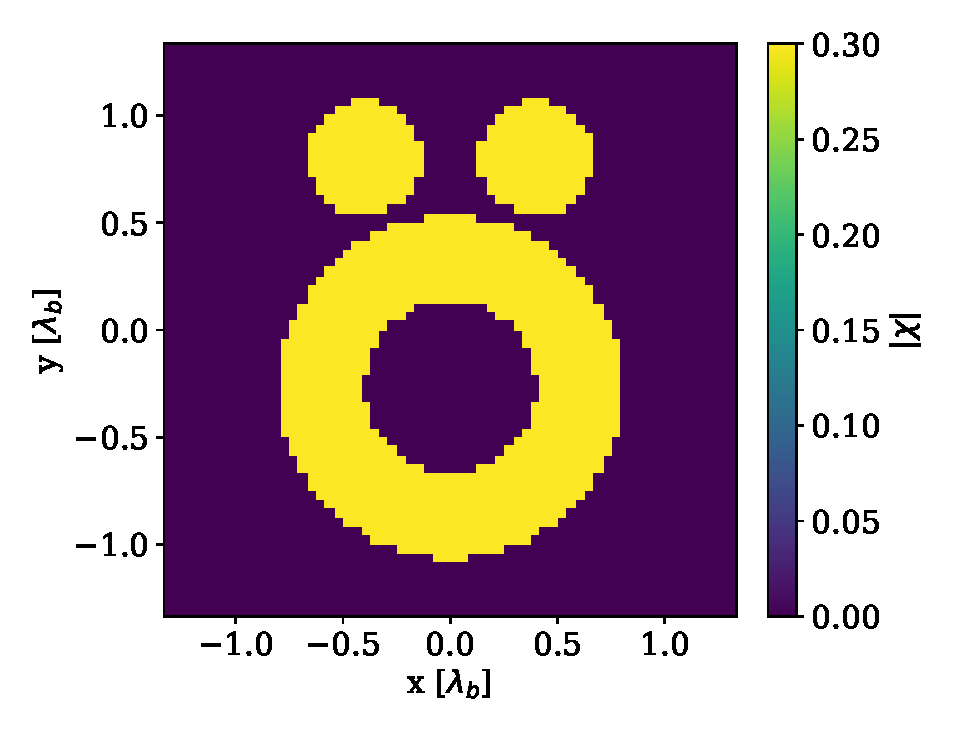
\includegraphics[width=.25\textwidth]{./figuras/casestudy/austria/groundtruth}\label{fig:results:casestudy:austria:reconstruction:groundtruth}}
				\subfloat[SAEA1]{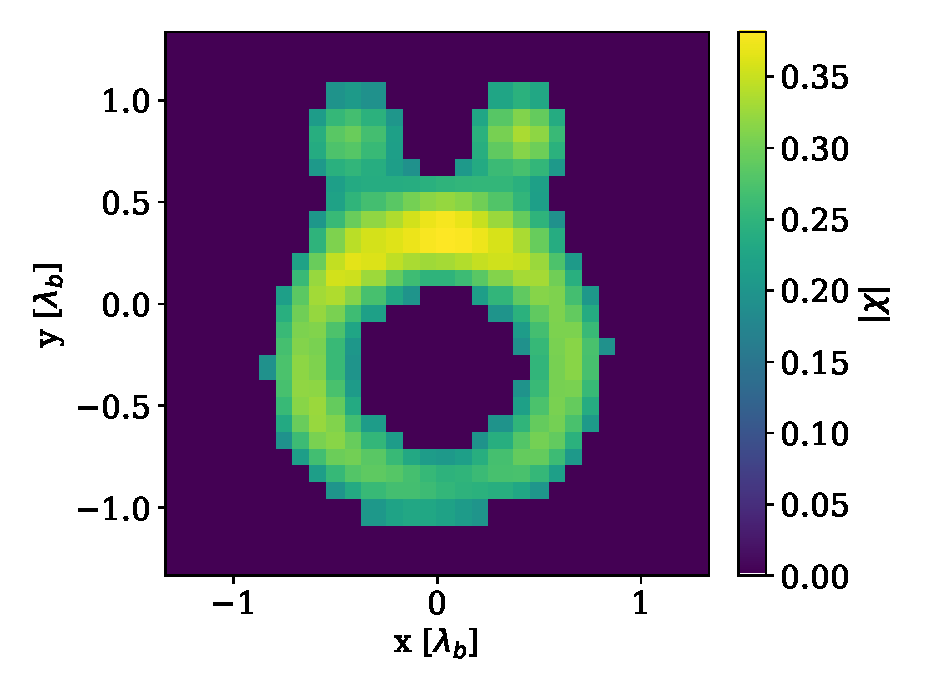
\includegraphics[width=.25\textwidth]{./figuras/casestudy/austria/reconstruction_saea1}\label{fig:results:casestudy:austria:reconstruction:saea1}}
				\subfloat[SAEA2]{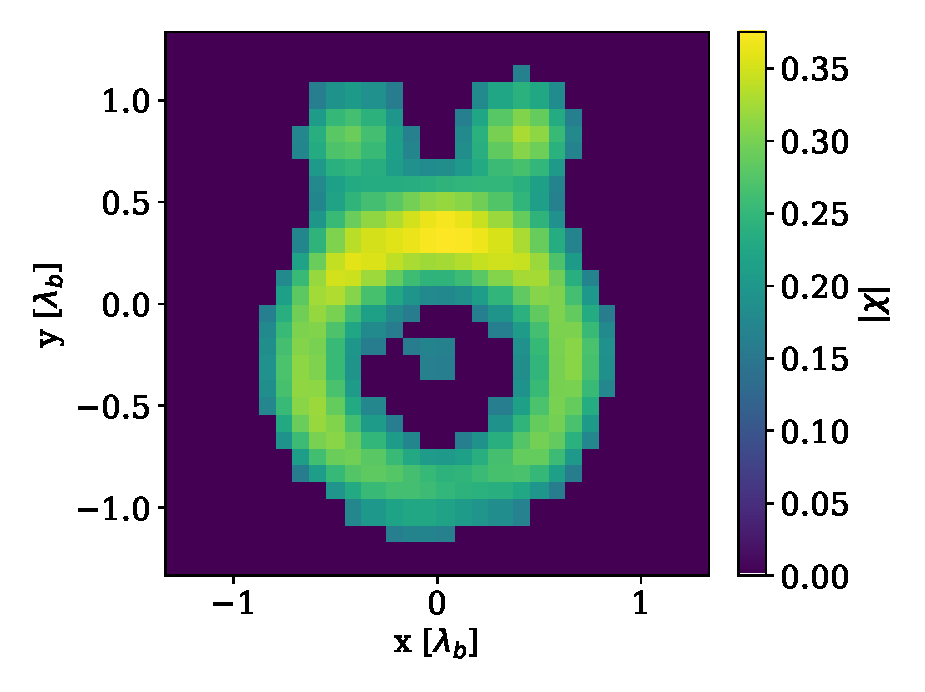
\includegraphics[width=.25\textwidth]{./figuras/casestudy/austria/reconstruction_saea2}\label{fig:results:casestudy:austria:reconstruction:saea2}}
				\subfloat[SAEA3]{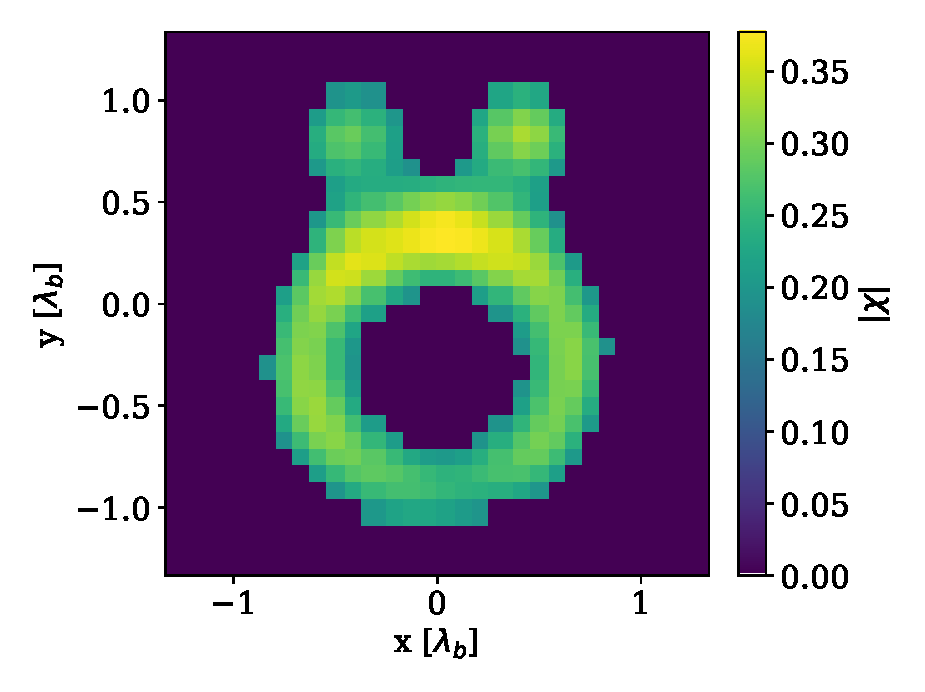
\includegraphics[width=.25\textwidth]{./figuras/casestudy/austria/reconstruction_saea3}\label{fig:results:casestudy:austria:reconstruction:saea3}} \\
				\subfloat[SADM1]{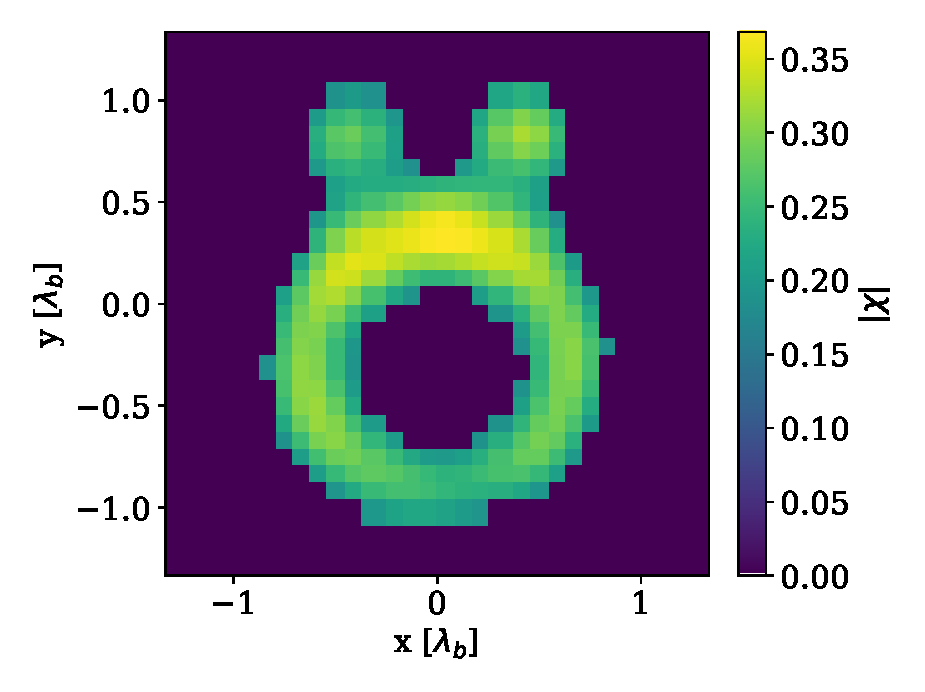
\includegraphics[width=.25\textwidth]{./figuras/casestudy/austria/reconstruction_sadm1}\label{fig:results:casestudy:austria:reconstruction:sadm1}}
				\subfloat[SADM2]{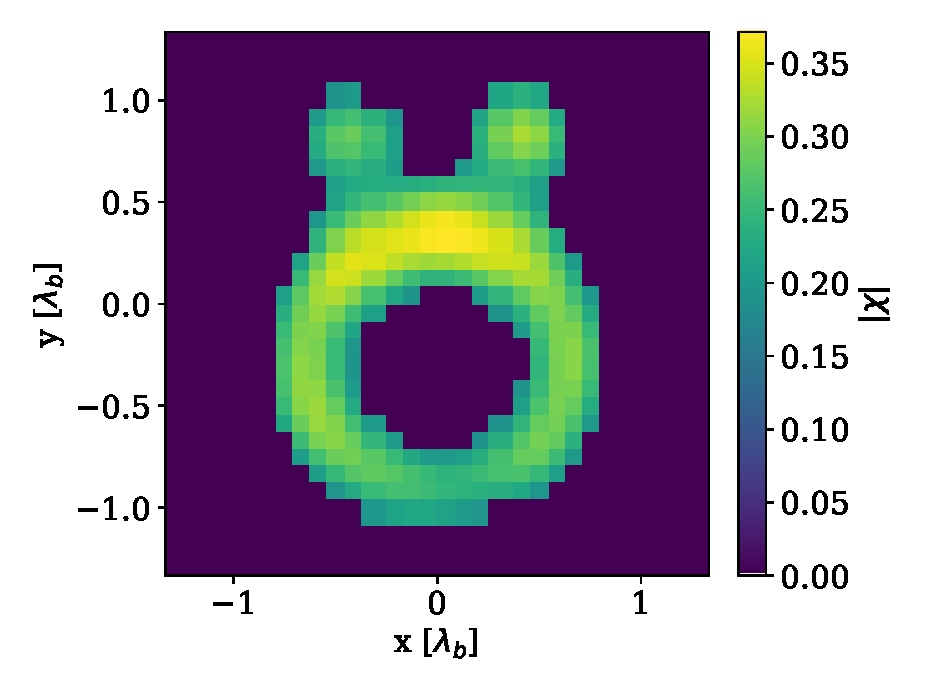
\includegraphics[width=.25\textwidth]{./figuras/casestudy/austria/reconstruction_sadm2}\label{fig:results:casestudy:austria:reconstruction:sadm2}}
				\subfloat[EA]{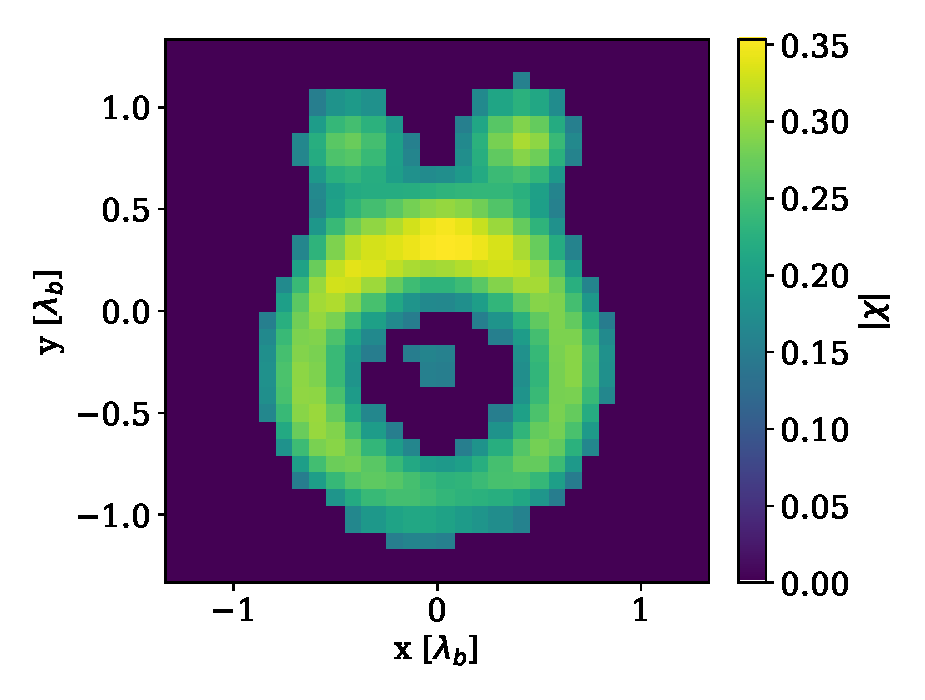
\includegraphics[width=.25\textwidth]{./figuras/casestudy/austria/reconstruction_ea}\label{fig:results:casestudy:austria:reconstruction:ea}}
				\subfloat[BIM]{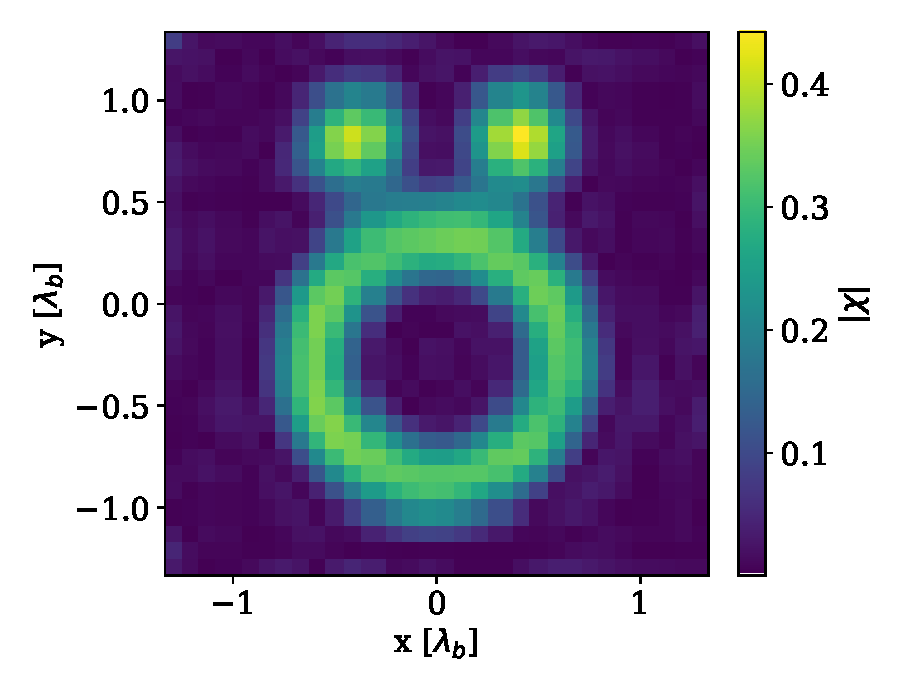
\includegraphics[width=.25\textwidth]{./figuras/casestudy/austria/reconstruction_bim}\label{fig:results:casestudy:austria:reconstruction:bim}} \\
				\subfloat[DBIM]{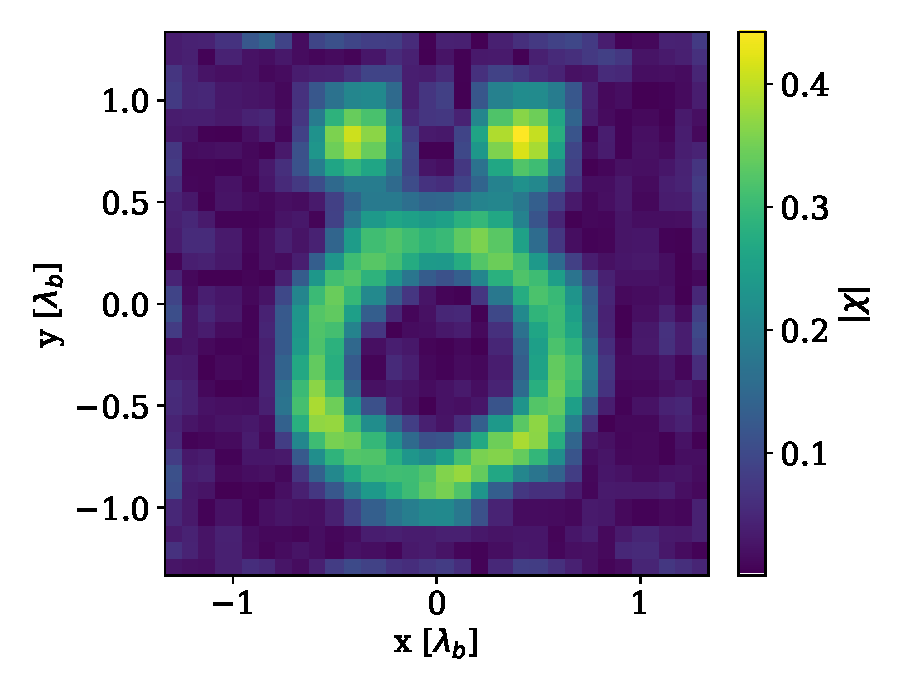
\includegraphics[width=.25\textwidth]{./figuras/casestudy/austria/reconstruction_dbim}\label{fig:results:casestudy:austria:reconstruction:dbim}}
				\subfloat[CGM]{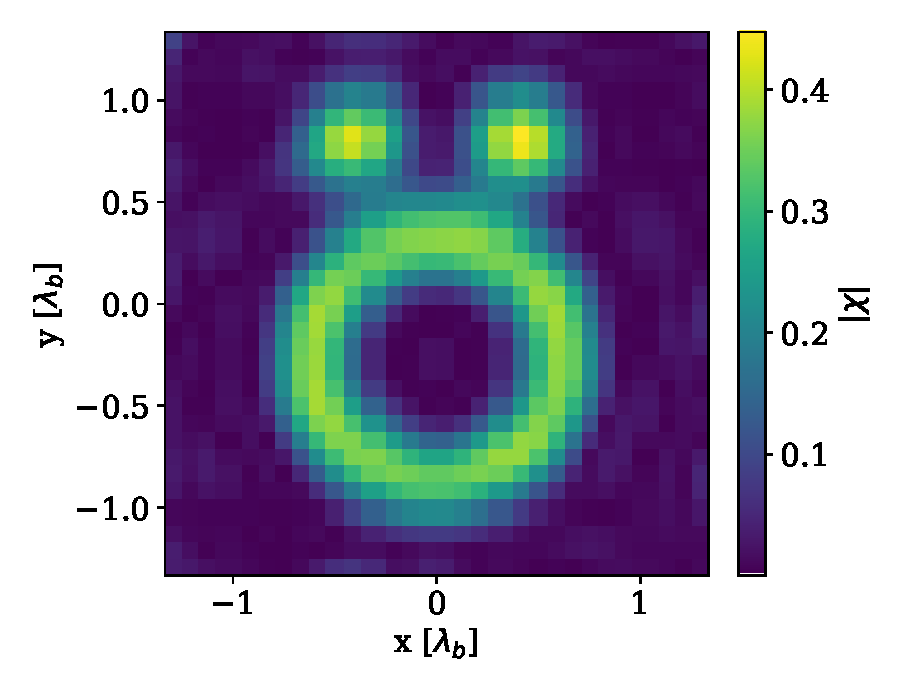
\includegraphics[width=.25\textwidth]{./figuras/casestudy/austria/reconstruction_cgm}\label{fig:results:casestudy:austria:reconstruction:cgm}}
				\subfloat[ECSI]{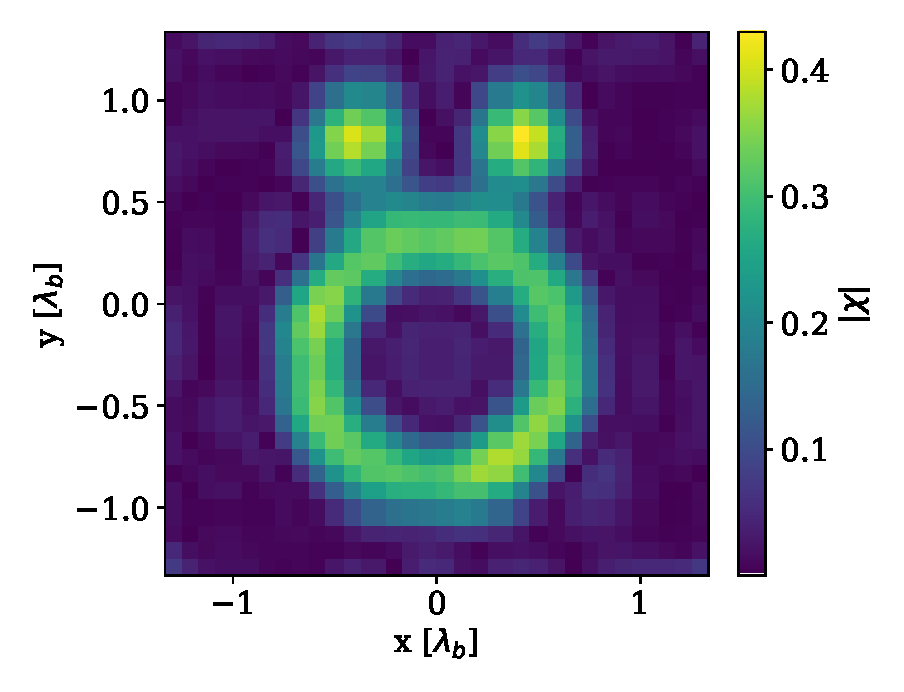
\includegraphics[width=.25\textwidth]{./figuras/casestudy/austria/reconstruction_ecsi}\label{fig:results:casestudy:austria:reconstruction:ecsi}}
				\subfloat[SOM]{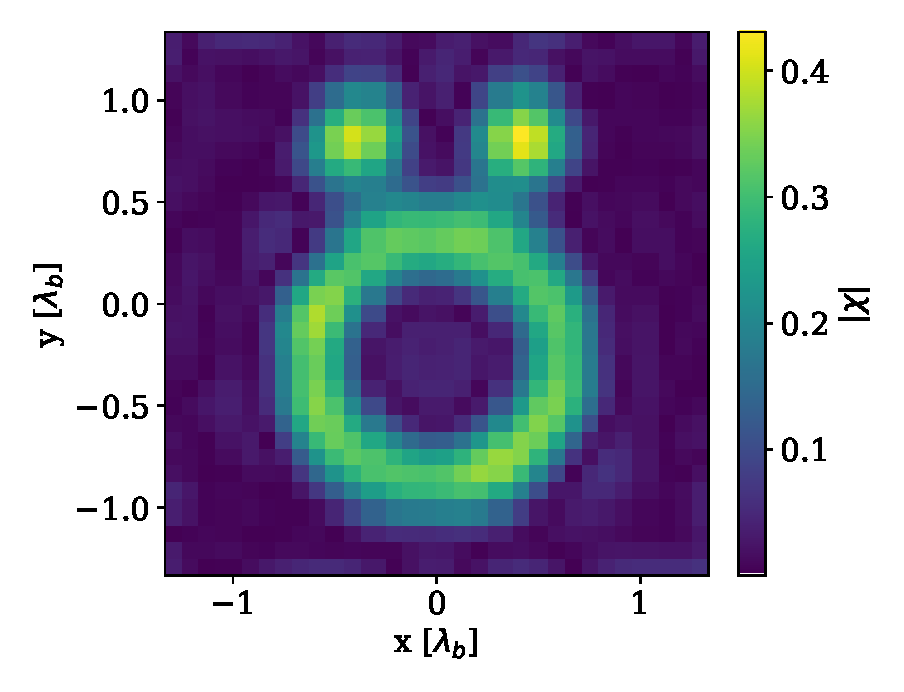
\includegraphics[width=.25\textwidth]{./figuras/casestudy/austria/reconstruction_som}\label{fig:results:casestudy:austria:reconstruction:som}} 
				\caption[Austria profile case study: Comparison of image reconstructions using surrogate model-assisted algorithms and deterministic methods.]{Comparison of image reconstructions using surrogate model-assisted algorithms and deterministic methods considering the Austria profile case study: (a) shows the ground-truth image; (b), (c), and (d) depict the best image recovered by SAEA1, SAEA2, and SAEA3, respectively, in 30 execution according to $\zeta_{\epsilon OE}$ indicator; (e), (f) and (g) show the best image recovered by SADM1, SADM2, and EA, respectively, in 30 execution according to $\zeta_{\epsilon OE}$ indicator; (g) shows the image recovered by BIM, and (h) shows the image recovered by DBIM; finally, (i), (k), and (l) show the image recovered by CGM, ECSI, and SOM, respectively.}
				\label{fig:results:casestudy:austria:reconstruction}
			\end{figure}
		
			% 1. A Fig. \ref{fig:results:casestudy:austria:reconstruction} mostra a melhor das reconstruções dentre as 30 execuções de cada algoritmo estocástico, de acordo com o indicador $\zeta_{\epsilon OE}$ (Figs. \ref{fig:results:casestudy:austria:reconstruction:saea1}-\ref{fig:results:casestudy:austria:reconstruction:ea}).
			% 2. A figura também mostra as reconstruções dos algoritmos determinísticos (Figs. \ref{fig:results:casestudy:austria:reconstruction:bim}-\ref{fig:results:casestudy:austria:reconstruction:som}).
			% 3. Todos os algoritmos fizeram uma ligeira superestimativa do contraste, conforme indica o valor máximo de contraste em cada figura. Essa suppdferestimativa tende a ser ligeiramente menor nos algoritmos baseados na proposta de transformação do problema. Este efeito tende a ser uma compensação pela subestimativa nas bordas do espalhador.
			% 4. Eles mostram também uma certa dificuldade em detectar bem a separação entre o anel e os dois círculos. Essa dificuldade está relacionada com a proximidade entre esses objetos.
			% 4. As melhores imagens reconstruídas pelo SAEA2 e pelo EA mostram um pequeno objeto fantasma dentro do anel da imagem. Isso é um problema do ajuste do valor do limiar. Como o indicador $\zeta_{\epsilon OE}$ só leva em consideração a estimativa dentro da região original do espalhador, então erros na região de fundo original do problema não são levados em conta.
			% 5. Como era de se esperar, os algoritmos baseados na transformação do problema em um de otimização bidimensional mostram uma região de fundo mais limpa. Isto é devido ao operador de limiarização. O BIM (Fig. \ref{fig:results:casestudy:austria:convergence:bim}) também apresenta uma região de fundo um pouco mais limpa que o DBIM (Fig. \ref{fig:results:casestudy:austria:convergence:dbim}) e isso está associado à dificuldade do DBIM com níveis de ruído significativos.
			
			In the results of the case study, Fig. \ref{fig:results:casestudy:austria:reconstruction} displays the best of the reconstructions among the 30 runs of each stochastic algorithm, based on indicator $\zeta_{\epsilon OE}$ (Figs. \ref{fig:results:casestudy:austria:reconstruction:saea1}-\ref{fig:results:casestudy:austria:reconstruction:ea}), and also includes the reconstructions of the deterministic algorithms (Figs. \ref{fig:results:casestudy:austria:reconstruction:bim}-\ref{fig:results:casestudy:austria:reconstruction:som}). The figures show that all algorithms overestimated the contrast slightly, which can be seen in the maximum contrast value in each figure. However, algorithms based on the problem transformation proposal tended to have slightly lower overestimation, which compensates for underestimation at the edges of the scatterer. The reconstructions also had some difficulty in detecting the separation between the ring and the two circles, which was related to the proximity between these objects. Additionally, the best SAEA2 and EA reconstructed images showed a small ghost object inside the image ring due to a threshold value adjustment issue. As the $\zeta_{\epsilon OE}$ indicator only takes into account the estimate within the original region of the scatterer, then errors in the original background region of the problem do not influence the indicator. Furthermore, algorithms based on transforming the problem into a two-dimensional optimization problem showed a cleaner background region, which was attributed to the thresholding operator. BIM (Fig. \ref{fig:results:casestudy:austria:convergence:bim}) presented a slightly cleaner background region than DBIM (Fig. \ref{fig:results:casestudy:austria:convergence:dbim}), which was associated with the difficulty of DBIM in dealing with significant noise levels.
		
			\begin{figure}[!h]
				\centering
				\subfloat[SAEA1]{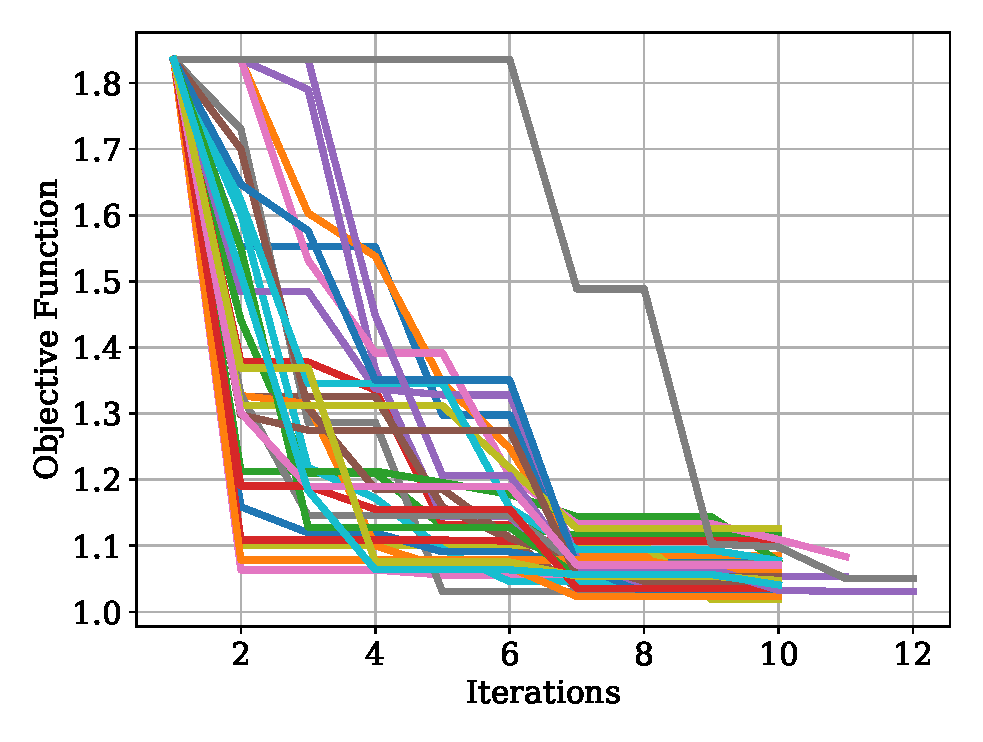
\includegraphics[width=.25\textwidth]{./figuras/casestudy/austria/convergence_saea1}\label{fig:results:casestudy:austria:convergence:saea1}}
				\subfloat[SAEA2]{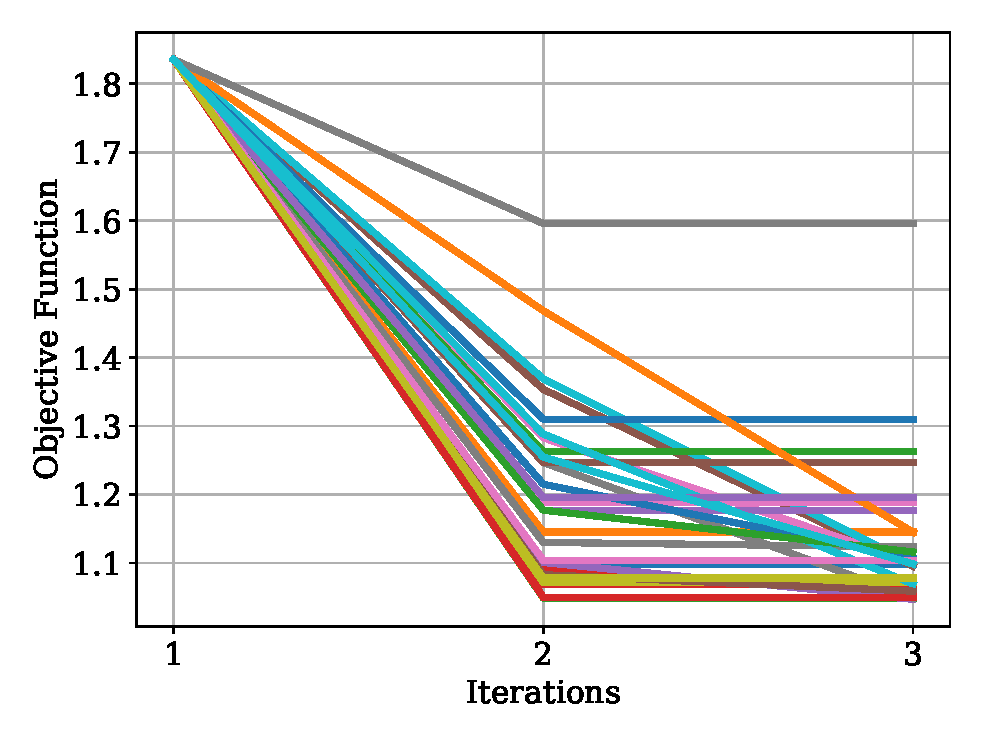
\includegraphics[width=.25\textwidth]{./figuras/casestudy/austria/convergence_saea2}\label{fig:results:casestudy:austria:convergence:saea2}}
				\subfloat[SAEA3]{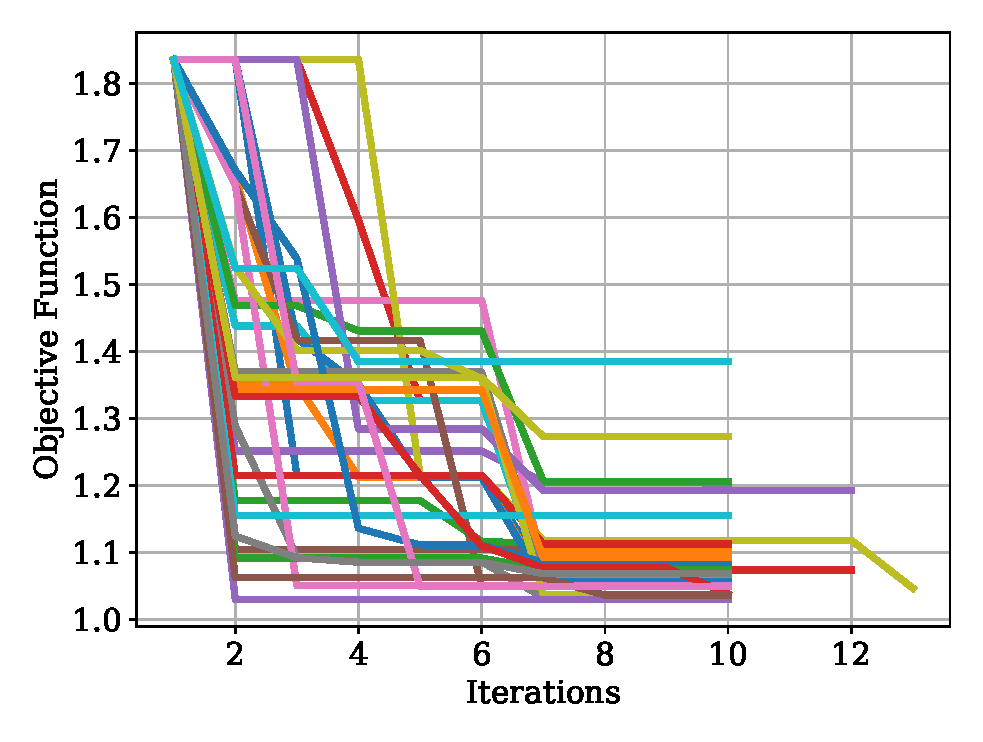
\includegraphics[width=.25\textwidth]{./figuras/casestudy/austria/convergence_saea3}\label{fig:results:casestudy:austria:convergence:saea3}}
				\subfloat[SADM1]{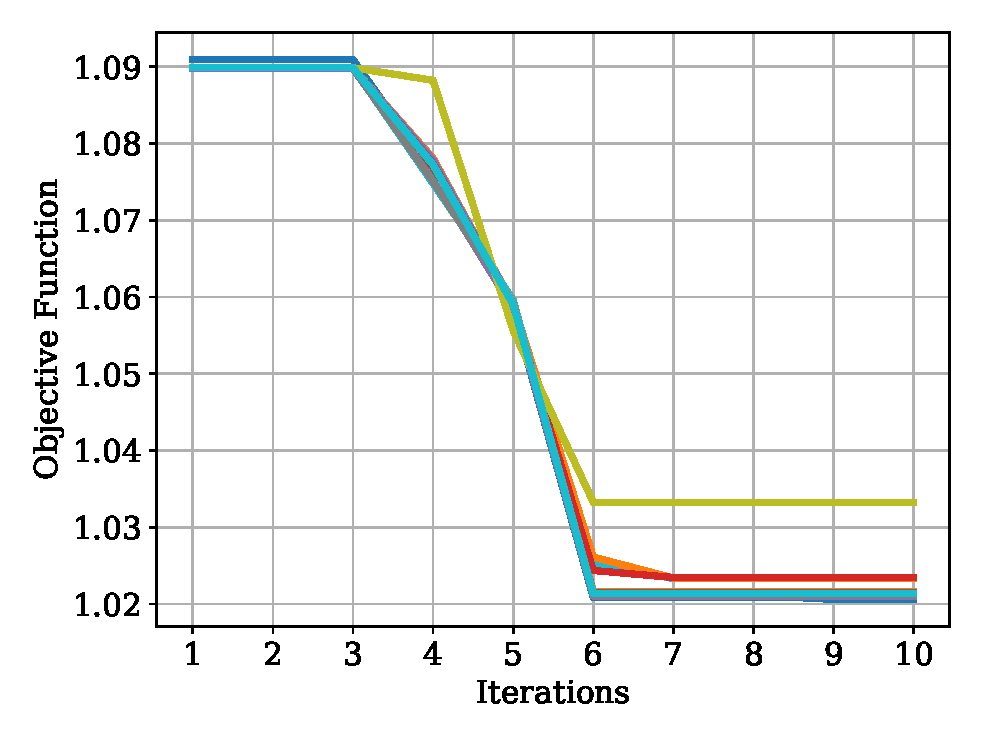
\includegraphics[width=.25\textwidth]{./figuras/casestudy/austria/convergence_sadm1}\label{fig:results:casestudy:austria:convergence:sadm1}} \\
				\subfloat[SADM2]{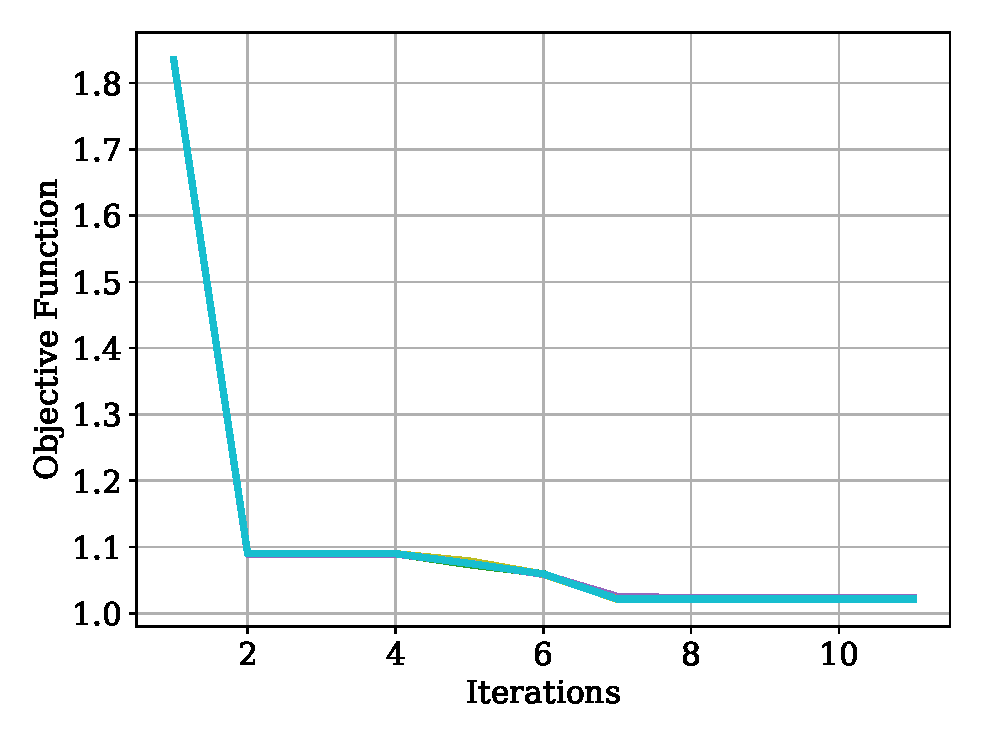
\includegraphics[width=.25\textwidth]{./figuras/casestudy/austria/convergence_sadm2}\label{fig:results:casestudy:austria:convergence:sadm2}}
				\subfloat[EA]{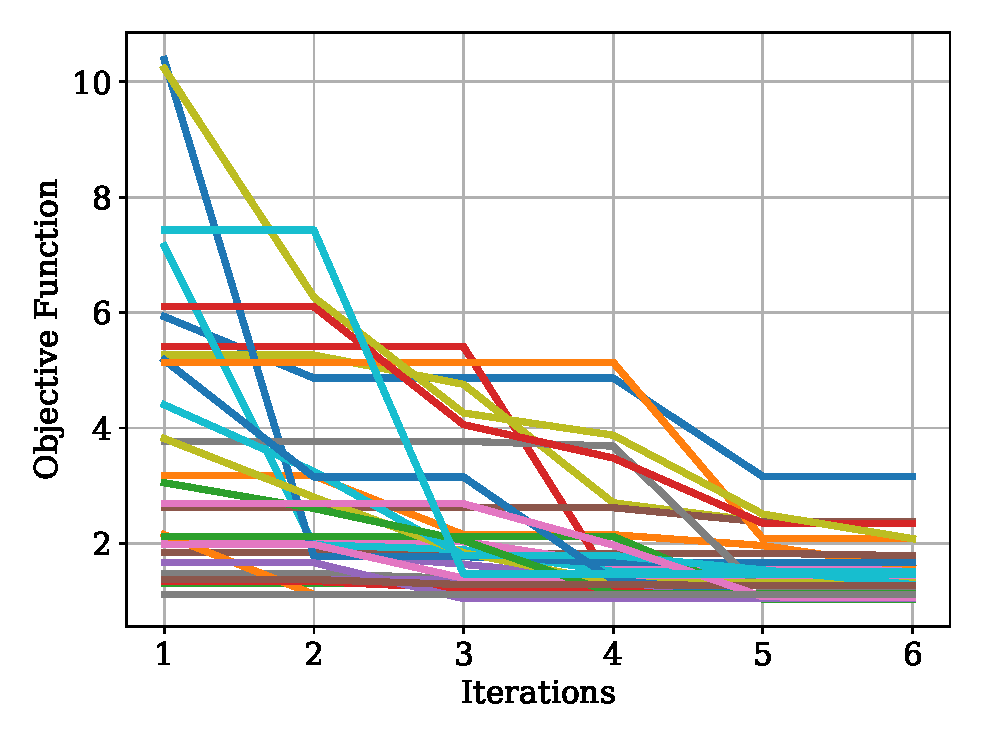
\includegraphics[width=.25\textwidth]{./figuras/casestudy/austria/convergence_ea}\label{fig:results:casestudy:austria:convergence:ea}}
				\subfloat[BIM]{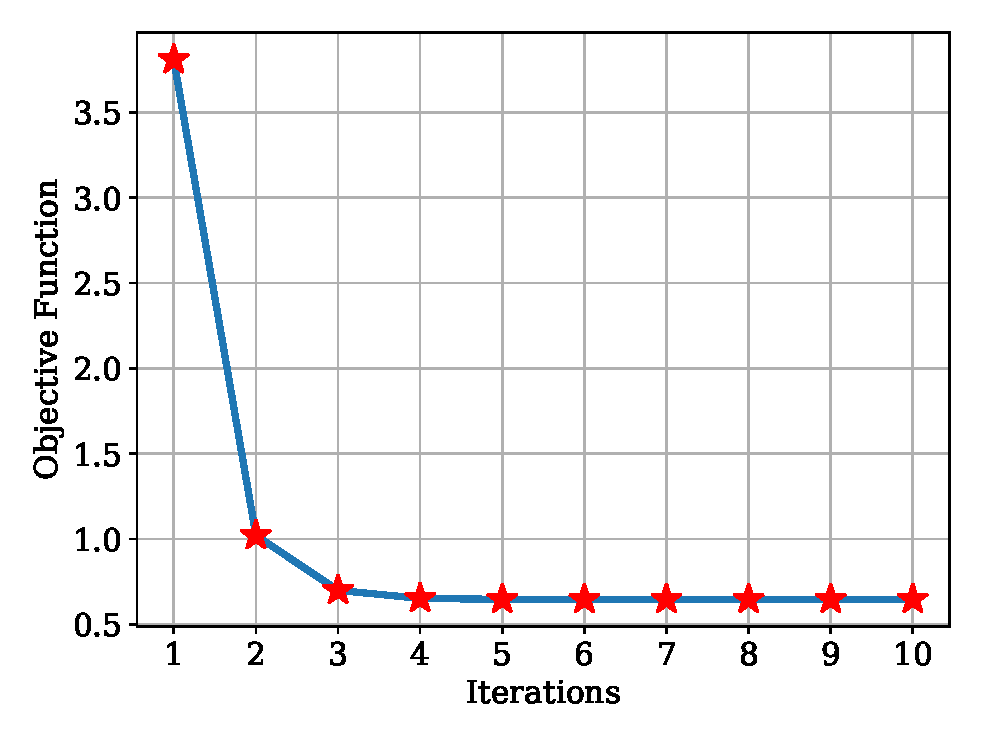
\includegraphics[width=.25\textwidth]{./figuras/casestudy/austria/convergence_bim}\label{fig:results:casestudy:austria:convergence:bim}}
				\subfloat[DBIM]{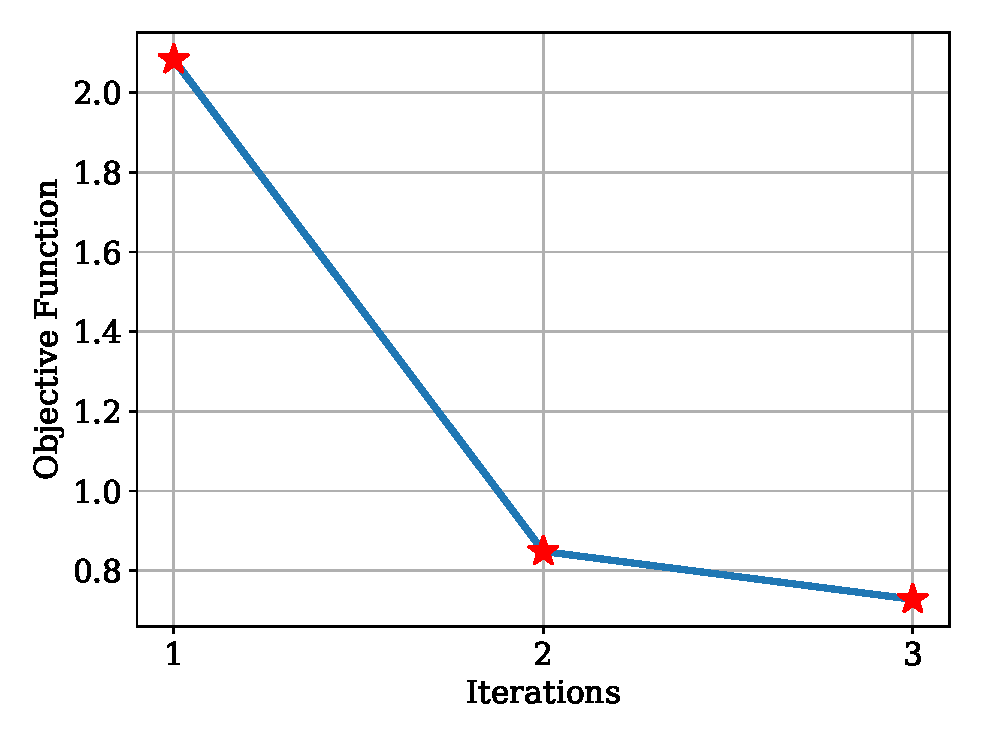
\includegraphics[width=.25\textwidth]{./figuras/casestudy/austria/convergence_dbim}\label{fig:results:casestudy:austria:convergence:dbim}} \\
				\subfloat[CGM]{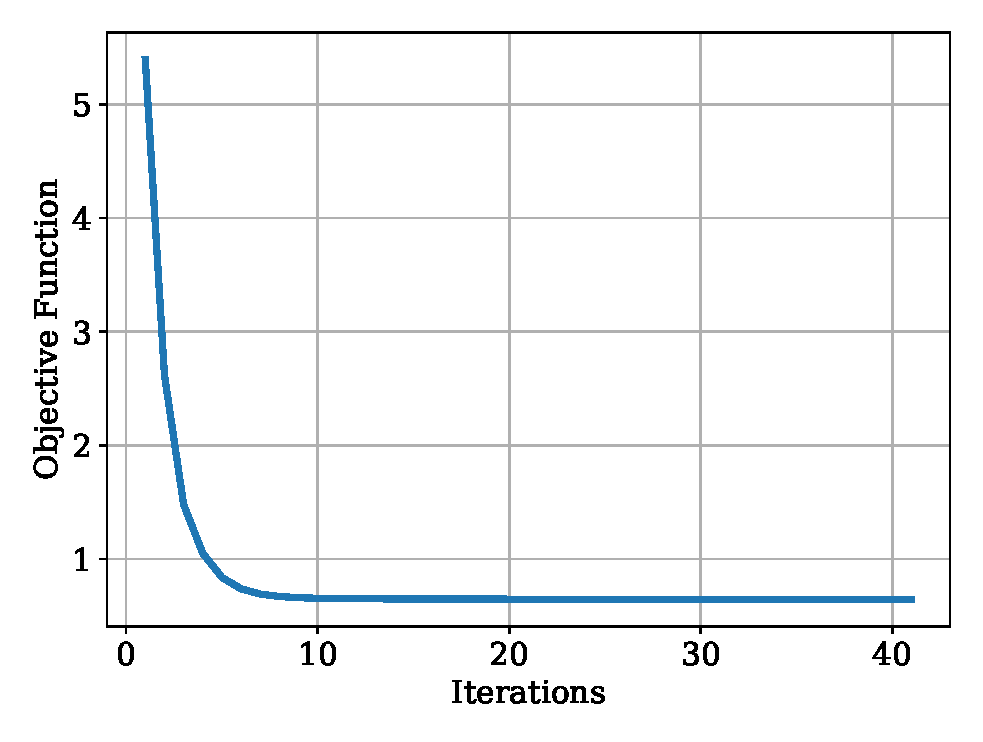
\includegraphics[width=.25\textwidth]{./figuras/casestudy/austria/convergence_cgm}\label{fig:results:casestudy:austria:convergence:cgm}}
				\subfloat[ECSI]{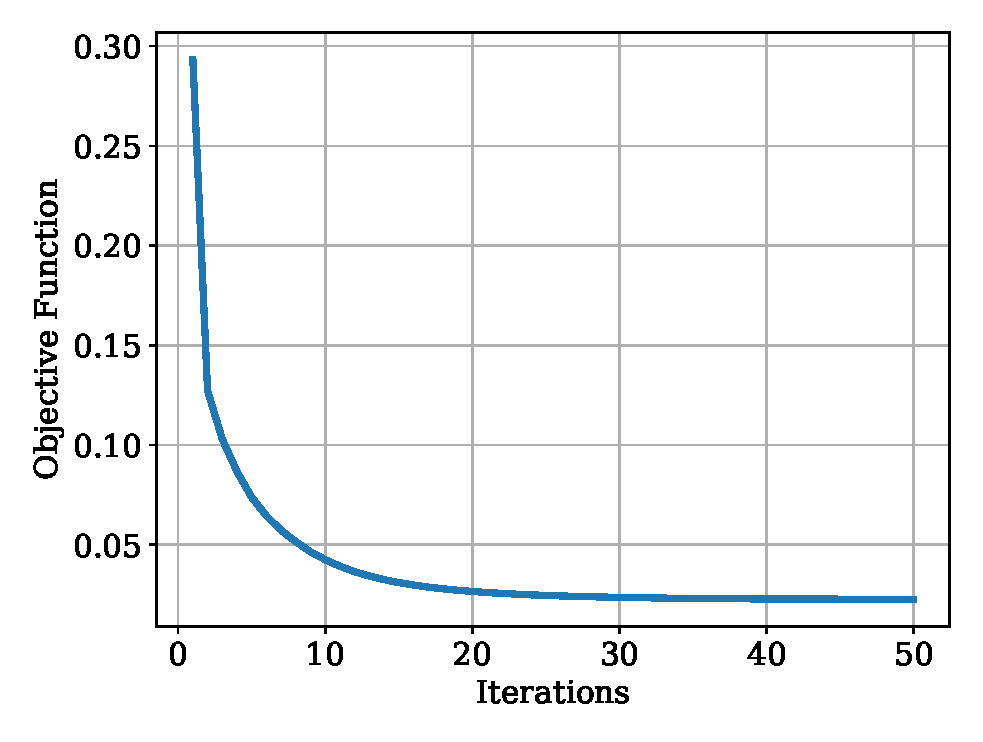
\includegraphics[width=.25\textwidth]{./figuras/casestudy/austria/convergence_ecsi}\label{fig:results:casestudy:austria:convergence:ecsi}}
				\subfloat[SOM]{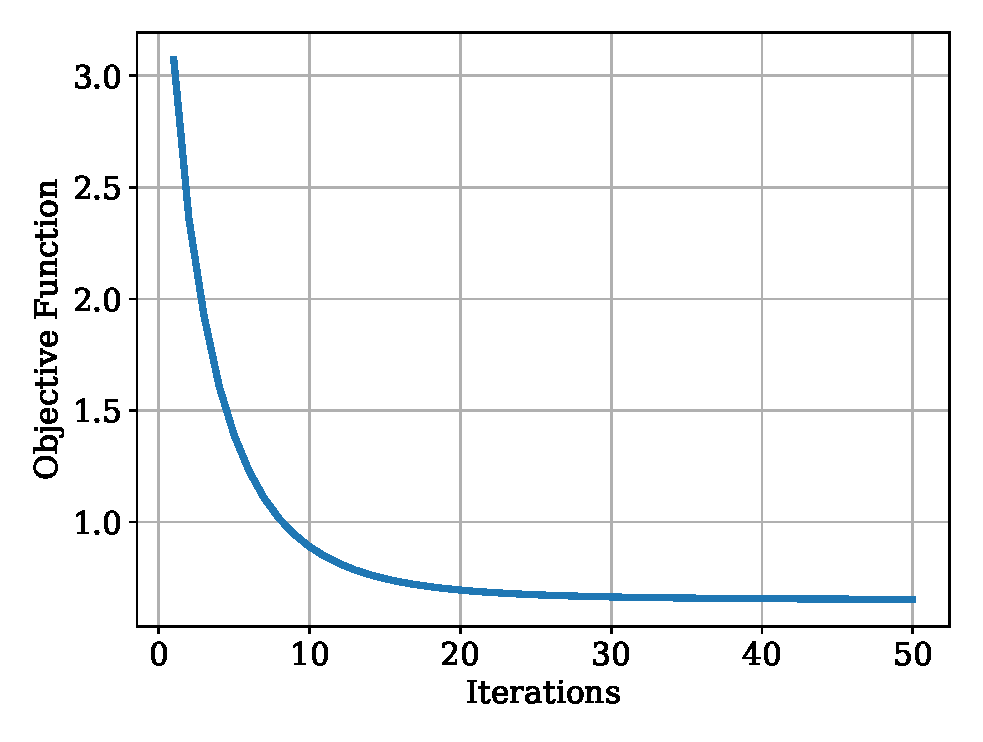
\includegraphics[width=.25\textwidth]{./figuras/casestudy/austria/convergence_som}\label{fig:results:casestudy:austria:convergence:som}} 
				\caption[Convergence of the objective function for the Austria profile case obtained by the stochastic and deterministic algorithms.]{Convergence of the objective function for the Austria profile case obtained by the stochastic and deterministic algorithms. (a) to (k) show the curves obtained by SAEA1, SAEA2, SAEA3, SADM1, SADM2, EA, BIM, DBIM, CGM, ECSI, and SOM algorithms, respectively. The x-axis represents the number of iterations, and the y-axis represents the value of the objective function of the correspondent algorithm.}
				\label{fig:results:casestudy:austria:convergence}
			\end{figure}
		
			% 1. A Fig. \ref{fig:results:casestudy:austria:convergence} mostra a curva de convergência da função-objetivo para cada algoritmo.
			% 2. Como cada algoritmo determinístico tem sua própria função-objetivo que pauta a sua estrutura, o eixo y só pode ser comparado entre os algoritmos baseados na otimização bidimensional (Figs. \ref{fig:results:casestudy:austria:convergence:saea1}-\ref{fig:results:casestudy:austria:convergence:ea}).
			% 3. O SAEA3 teve somente 3 gerações. O número baixo é explicado pelo fato de que cada iteração o número de avaliações da função-objetivo verdadeira é igual ao tamanho da população. Isto é diferente do SAEA1 e do SAEA3 que gastam somente uma avaliação por geração.
			% 4. Mesmo com poucas gerações, o SAEA2 ainda assim termina as execuções com valores próximos dos alcançados pelo SAEA1 e pelo SAEA3. Isso tem a ver com o bom mapeamento do espaço de busca feito pela população inicial.
			% 5. Os valores finais alcançados pelo SAEA1 nas 30 execuções foram mais semelhantes que os do SAEA3. Isto pode sugerir que a convergência do SAEA1 é melhor.
			% 6. Algumas execuções do SADM1 não convergiram para o mesmo local que a maioria. Isto pode ser um efeito do processo estocástico de busca por solução inicial. O mesmo não acontece para o SADM2. Todas as execuções desse algoritmo convergiram igualmente, indicando um comportamento determinístico.
			% 7. O EA tem mais gerações que o SAEA2 porque o EA não tem a necessidade de gerar uma amostra inicial de soluções. No entanto, o número maior de gerações não contribuiu para alcançar mais rapidamente a região perto do mínimo. Isso é mais factível para o SAEA2 por causa da estratégia de amostragem de soluções.
			
			The convergence curve for each algorithm is shown in Fig. \ref{fig:results:casestudy:austria:convergence}. The y-axis can only be compared between algorithms based on two-dimensional optimization (Figs. \ref{fig:results:casestudy:austria:convergence:saea1}-\ref{fig:results:casestudy:austria:convergence:ea}), as each deterministic algorithm has its own objective function that guides its structure. SAEA2 had a few generations but still achieved values close to those achieved by SAEA1 and SAEA3, thanks to the good mapping of the search space done by the initial population. The final values reached by SAEA1 in the 30 runs were more similar than those by SAEA3, which may suggest that SAEA1 convergence is better.
			
			Some SADM1 runs did not converge to the same location as most, which may be an effect of the stochastic search process for the initial solution. The same does not happen for SADM2, as all executions of this algorithm converged equally, indicating a deterministic behavior. The EA has more generations than the SAEA2, but the greater number of generations did not contribute to reaching the region closer to the minimum more quickly. This is straightforward for SAEA2 because of the solution sampling strategy.			
		
			\begin{figure}
				\centering
				\subfloat[]{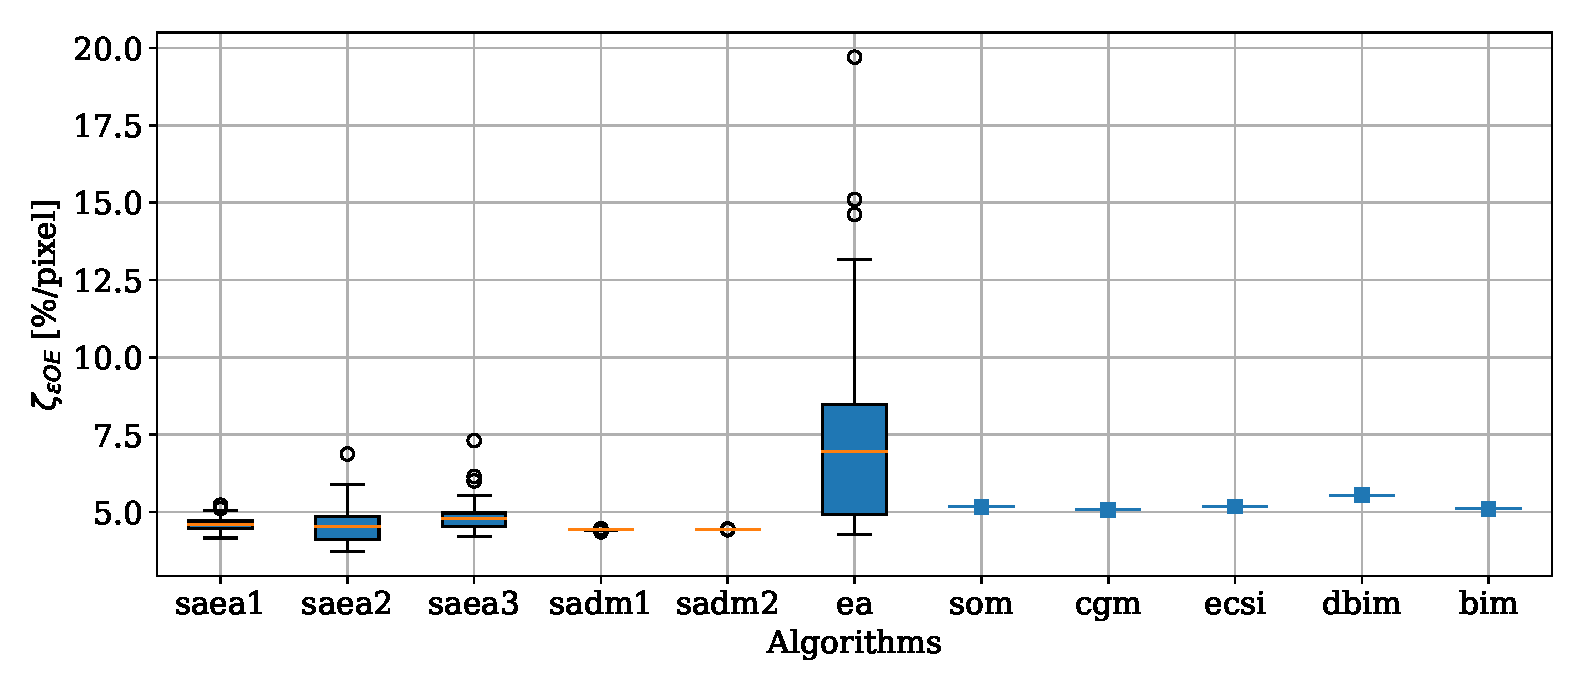
\includegraphics[width=.9\textwidth]{./figuras/casestudy/austria/boxplot_zeta_eoe_ea}\label{fig:results:casestudy:austria:boxplot:zeta_eoe:withea}} \\
				\subfloat[]{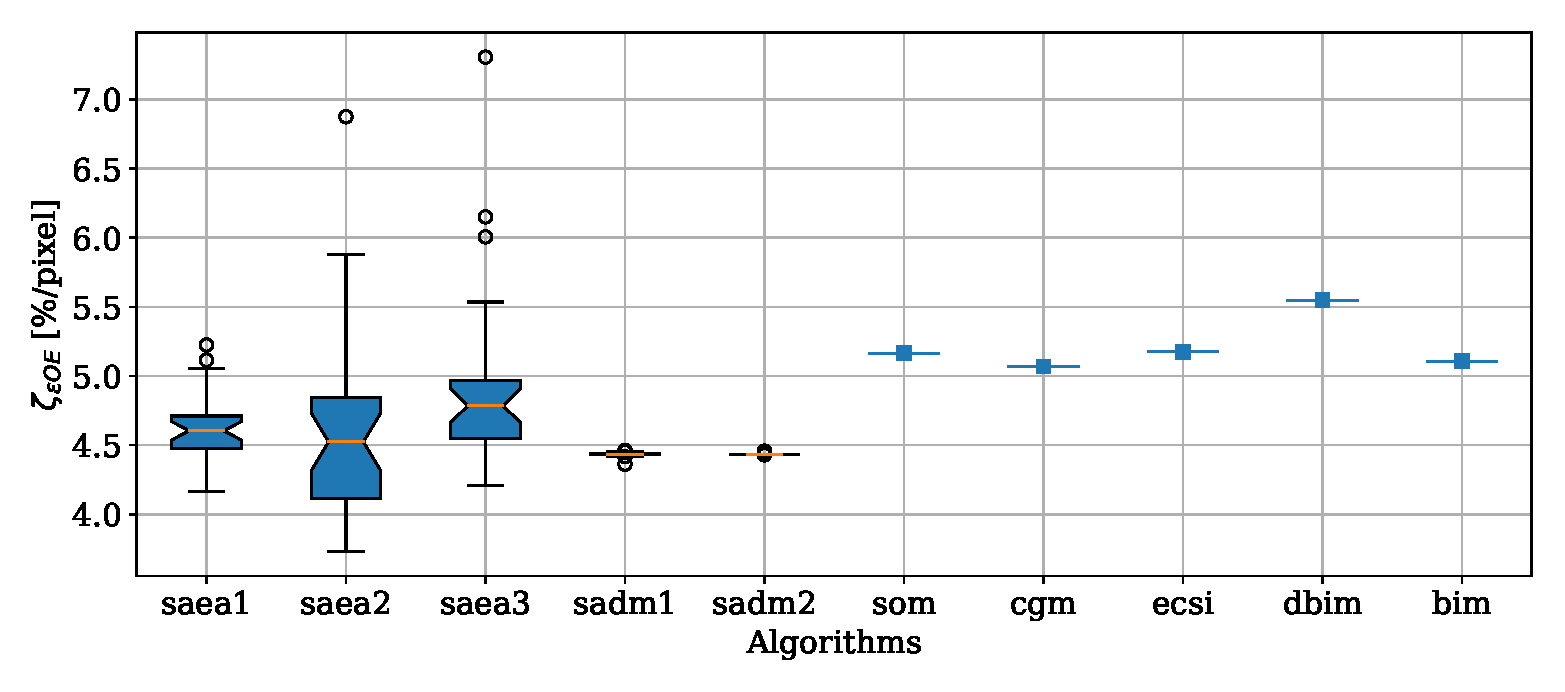
\includegraphics[width=.9\textwidth]{./figuras/casestudy/austria/boxplot_zeta_eoe}\label{fig:results:casestudy:austria:boxplot:zeta_eoe:noea}}
				\caption[Performance of $\zeta_{\epsilon OE}$ indicator for various algorithms in the Austria profile.]{Performance of $\zeta_{\epsilon OE}$ indicator for various algorithms in the Austria profile. (a) Boxplots show quartiles of 30 executions for stochastic algorithms, and the solid line represents the deterministic algorithms. (b) Exclusion of the EA algorithm for better visualization of differences among algorithms.}
				\label{fig:results:casestudy:austria:boxplot:zeta_eoe}
			\end{figure}
		
			% 1. A Fig. \ref{fig:results:casestudy:austria:boxplot:zeta_eoe:withea} mostra os quartis do indicador $\zeta_{\epsilon OE}$ para os algoritmos nos quais foram executadas 30 execuções e o valor alcançados pelos determinísticos.
			% 2. Os quartis do EA se destacam negativamente. Tal dificuldade por encontrar uma boa estimativa final do contraste do espalhador tem a ver com a necessidade que o algoritmo tem de mais gerações para poder convergir para mais perto do ótimo, como nos outros algoritmos assistidos por modelos substitutos.
			% 3. Removendo os dados do EA (Fig. \ref{fig:results:casestudy:austria:boxplot:zeta_eoe:noea}), é possível visualizar melhor as diferenças entre os algoritmos assistidos por modelos substitutos e os determinísticos. A mediana dos algoritmos assistidos por modelos substitutos ficaram abaixo de todos os determinísticos. Em especial, todas as execuções do SADM1 e do SADM2 ficaram abaixo do erro de estimativa de contraste dos determinísticos. No entanto, houveram execuções dos SAEA's que terminaram com um erro menor.
			% 4. Todas as execuções do SADM2 terminaram com o mesmo erro, uma vez que todas as execuções convergiram de igual modo (conforme visto na Fig. \ref{fig:results:casestudy:austria:convergence:sadm2}). Embora a convergência do SADM1 não tenha sido tão igual entre as execuções, eles alcançaram o mesmo erro. Isso indica que a solução final de cada execução foi muito próxima.
			% 5. O erro da estimativa de contraste dos algoritmos assistidos por modelos substitutos tem a ver com o local da superfície de otimização no qual eles terminam.
			% 6. De uma maneira geral, o resultado indica que a abordagem de transformação do problema pode ser bem sucedida de forma a fazer uma estimativa de contraste melhor na mediana dos casos, comparando com as abordagens tradicionais. No entanto, em cenários de espalhadores fracos, essa diferença não é tão significativa conforme mostra os gráficos (até 1.5 [\%/pixel]).
			
			Fig. \ref{fig:results:casestudy:austria:boxplot:zeta_eoe:withea} shows the $\zeta_{\epsilon OE}$ indicator quartiles for the algorithms in which 30 executions were performed and the value reached by the deterministic ones. The EA quartiles stand out negatively, as the algorithm has difficulty finding a good final estimate of the scatterer contrast. This is attributed to the algorithm's need for more generations to converge closer to the optimum, as in other algorithms assisted by surrogate models.
			
			By removing the EA data (Fig. \ref{fig:results:casestudy:austria:boxplot:zeta_eoe:noea}), it is possible to better visualize the differences between the algorithms assisted by surrogate models and the deterministic ones. The median of algorithms assisted by surrogate models was below all deterministic ones. In particular, all SADM1 and SADM2 runs were below the deterministic contrast estimation error. However, there have been executions of SAEA's that ended with a minor error. All runs of SADM2 ended with the same error since all runs converged equally (as seen in Fig. \ref{fig:results:casestudy:austria:convergence:sadm2}). Although SADM1 convergence was not as equal between runs, they achieved the same error, indicating that the final solution for each run was very close. The Kruskal-Wallis H-Test confirmed difference among SAEA1, SAEA2, and SAEA3 (p-value $=0.0219$), and all-to-all comparison by Mann-Whitney U test confirmed that SAEA1 and SAEA2 overperformed SAEA3 (p-values 0.0199 and 0.0191, respectively). The Multiple Mann-Whitney U test did not detected difference between SADM1 and SADM2 (p-value $=0.0505$).
			
			The contrast estimation error of surrogate model-assisted algorithms has to do with where on the optimization surface they end up. In general, the result indicates that the problem transformation approach can be successful in making a better contrast estimate in the median of cases compared to the traditional approaches. However, in weak scattering scenarios, this difference is not as significant as the graphs show (up to 1.5 [\%/pixel]).
		
			\begin{figure}
				\centering
				\includegraphics[width=.9\textwidth]{./figuras/casestudy/austria/boxplot_zeta_s}
				\caption[Performance of shape error estimation quantified by the $\zeta_S$ indicator obtained by the set of algorithms considering the Austria profile.]{Performance of shape error estimation quantified by the $\zeta_S$ indicator obtained by the set of algorithms considering the Austria profile. The boxes represent the quartiles of the 30 executions of the stochastic algorithms, while the other points indicate the obtained values by the deterministic ones. The shape error is calculated based on the ground-truth image and the reconstructed image obtained by each algorithm.}
				\label{fig:results:casestudy:austria:boxplot:zeta_s}
			\end{figure}
		
			% 1. Em relação ao erro de recuperação de forma $\zeta_S$ (Fig. \ref{fig:results:casestudy:austria:boxplot:zeta_s}), a diferença de desempenho é mais significativa entre os algoritmos determinísticos e aqueles baseados na transformação do problema. A diferença pode ser de até 20\%, aproximadamente, da área do espalhador original.
			% 2. O sucesso da abordagem de transformação proposta nos resultados de recuperação de forma está associado tanto à qualidade dos métodos qualitativos em fazer essa estimativa quanto na eficiência da operação de limiarização intrínseca à formulação.
			
			The performance of different algorithms for shape recovery error ($\zeta_S$) is shown in Fig. \ref{fig:results:casestudy:austria:boxplot:zeta_s}. The difference in performance between deterministic algorithms and those based on the transformation of the problem is more significant, up to approximately 20\% of the area of the original scatterer. The success of the proposed transformation approach in shape recovery results is associated with the quality of the qualitative methods used and the efficiency of the thresholding operation intrinsic to the formulation. The Kruskal-Wallis H-Test confirmed difference among SAEA1, SAEA2, and SAEA3 (p-value $<0.0002$), and all-to-all comparison by Multiple Mann-Whitney U test confirmed that SAEA1 and SAEA2 overperformed SAEA3 (p-values $<0.001$ for both cases). The Mann-Whitney U test detected difference suggesting that SADM1 outperform SADM2 (p-value $=0.013$).
		
			\begin{figure}
				\centering
				\includegraphics[width=.9\textwidth]{./figuras/casestudy/austria/boxplot_time}
				\caption[Box plot showing the execution time distribution of the set of algorithms considered for the Austria profile case.]{Box plot showing the execution time distribution of the set of algorithms considered for the Austria profile case. The boxes represent the quartiles of the 30 executions of the stochastic algorithms, and the whiskers represent the minimum and maximum values. The deterministic algorithms are represented by individual points. The execution time results are presented in seconds.}
				\label{fig:results:casestudy:austria:boxplot:time}
			\end{figure}
		
			% 1. A Fig. \ref{fig:results:casestudy:austria:boxplot:time} mostra o tempo de execução dos algoritmos.
			% 2. A mediana do SAEA1 foi a mais alta. Levando em conta somente as formulações do SAEA's, o SAEA2 foi o mais rápido, mesmo tendo o mesmo número de avaliações. Este resultado sugere o impacto de operações dentro do processo iterativo desses algoritmos, como o processo de busca local e o número de chamadas de treinamento do modelo que são menos acionados no SAEA2 para o mesmo número de avaliações.
			% 3. No entanto, vale à pena observar que os SADM's também precisam retreinar o modelo uma vez por iteração, também gastam uma avaliação por iteração e também fazem um uso do mesmo algoritmo que é aplicado para o processo de busca local no SAEA's. Logo, outros processos que fazem parte da implementação desses algoritmos também podem estar impactando o tempo de execução.
			% 4. É importante destacar também que, embora o BIM leve muito menos tempo que o SADM2, este último ainda consegue entregar bons resultados de estimativa de contraste e de forma por um tempo que é satisfatório (menor que 10 segundos) e menor que outros algoritmos como SOM, CGM e ECSI. Por isso, com um pouco mais de tempo, o SADM2 consegue entregar um resultado melhor nesta instância que é bem tratada por algoritmos tradicionais.
			
			The running time of the algorithms is shown in Fig. \ref{fig:results:casestudy:austria:boxplot:time}. The median of SAEA1 was found to be the highest, while SAEA2 was the fastest among SAEA's formulations, even with the same number of evaluations. This suggests the impact of operations within the iterative process of these algorithms, such as the local search process and the number of model training calls that are less triggered in SAEA2 for the same number of evaluations. However, it is important to note that SADMs also need to retrain the model once per iteration, spend one evaluation per iteration, and use the same algorithm applied for the local search process in SAEAs. Other processes that are part of the implementation of these algorithms may also be impacting the runtime. It is also worth highlighting that although BIM takes much less time than SADM2, the latter still manages to deliver good contrast and shape estimation results for a satisfactory time (less than 10 seconds), which is shorter than other algorithms such as SOM, CGM, and ECSI. Therefore, with a little more time, SADM2 can deliver a better result in this instance that is well-treated by traditional algorithms.
		
			\begin{figure}
				\centering
				\subfloat[]{\includegraphics[width=.45\textwidth]{./figuras/casestudy/austria/surface1}\label{fig:results:casestudy:austria:boxplot:surface:1}} \hspace{.05\textwidth}
				\subfloat[]{\includegraphics[width=.45\textwidth]{./figuras/casestudy/austria/surface2}\label{fig:results:casestudy:austria:boxplot:surface:2}}
				\caption[Surface of the two-dimensional optimization problem obtained from the transformation of the Austria profile and the final solutions obtained by different algorithms.]{Surface of the two-dimensional optimization problem obtained from the transformation of the Austria profile and the final solutions obtained by different algorithms. Subfigure (a) shows the final solutions obtained by SAEA1, SAEA2, and SADM1 algorithms, while subfigure (b) shows the final solutions obtained by EA, SAEA3, and SADM2 algorithms.}
				\label{fig:results:casestudy:austria:surface}
			\end{figure}
		
			% 1. A Fig. \ref{fig:results:casestudy:austria:surface} mostra a superfície da função-objetivo e a posição das soluções finais encontrada por cada algoritmo baseado na transformação do problema inverso em um de otimização bidimensional.
			% 2. Para uma superfície razoavelmente comportada no sentido macro, os SADM's se comportam como algoritmos determinísticos, uma vez que convergiram todas as vezes para o mesmo ponto.
			% 3. A figura mostra também o grande espalhamento das soluções do EA, indicando que o número de avaliações precisaria ser bem maior para que o algoritmo convergisse mais vezes para o local do ótimo.
			% 4. Os SAEA's tiveram um comportamento similar, exceto talvez pelo SAEA3 que ligeiramente se afastou mais do ponto encontrado pelos SADM's.
			% 5. É importante que soluções finais pouco mais distantes do ótimo podem retornar às vezes um erro menor de estimativa de contraste ou de recuperação de forma. Isso se dá pelo motivo que o ponto de ótimo do problema transformado pode ser um pouco deslocado daquilo que seria o ideal para o processo de limiarização e do valor exato de contraste. Esse deslocamento é intrínseco à estimativa do método qualitativo. Ou seja, a solução ótima do problema transformado não é necessariamente a exata, mas a melhor que posso obter a partir do método qualitativo e minimizando o erro da equação de dados. Por isso, a performance do método qualitativo influencia na posição do ótimo.
			
			Figure \ref{fig:results:casestudy:austria:surface} illustrates the performance of the algorithms, displaying both the objective function surface and the locations of the final solutions obtained by each algorithm after transforming the inverse problem into a two-dimensional optimization problem. The SADMs converged to the same point every time, indicating that they behaved like deterministic algorithms for a reasonably smooth surface in the macro sense. The EA solutions, on the other hand, were widely spread, indicating that the number of evaluations would need to be much higher for the algorithm to converge more often to the optimal location.
			
			The SAEA3 had a similar behavior to EA, which slightly moved away from the point found by the SADMs. However, it is important to note that final solutions that are a little farther from the optimum can sometimes return a smaller error in contrast estimation or shape recovery. This is because the optimal point of the transformed problem can be slightly displaced from what would be ideal for the thresholding process and the exact contrast value. This displacement is intrinsic to the estimation of the qualitative method. That is, the optimal solution of the transformed problem is not necessarily the exact one, but the best that can be obtained from the qualitative method and minimizing the error of the data equation. Therefore, the performance of the qualitative method influences the position of the optimum.
		
		\subsection{Multiple Scatterers}\label{chap:results:casestudy:multiple}
		
			% * Esta subseção discute um estudo de caso que considera múltiplos espalhadores.
			% * Esse tipo de cenário é importante pois permite investigar a capacidade de separar os objetos na imagem.
			% * Além disso, o contraste dos espalhadores será consideravelmente mais alto para explorar ainda mais o potencial da aplicação dos modelos substitutos.
			% * A descrição dos três espalhadores presentes no teste será feita a seguir. 
			% * Os três objetos tem contraste igual a 4.
			% * O raio do círculo é $0.1\lambda_b$ e está centrado nas coordenadas ($L_X/4$, $0$).
			% * O lado do quadrado é $0.2\lambda_b$ e está centrado nas coordenadas ($-L_Y/4$, $-L_X/4$).
			% * O lado do triângulo é $0.2\lambda_b$ e está centrado nas coordenadas ($-L_Y/4$, $L_X/4$).
			% * O DNL do problema ficou em 0.915, o que é perto do limiar 1 para o problema começa a ficar muito não-linear. Não chega a ser tanto um caso de espalhador forte.
			% * Os parâmetros que descrevem os domínios do problema estão presentes na Tabela 2.
			% * Todas as outras configurações de sintetização dos dados do campo espalhado são as mesmas do estudo de caso anterior, exceto que agora a resolução da imagem original é 120$\times$120.
	
			This subsection presents a case study that examines the ability to separate objects in an image when considering multiple scatterers. This type of scenario is significant and, in order to further explore the application potential of the surrogate models, the contrast of the scatterers will be considerably higher. The study describes three scatterers that have a contrast level equal to 4. The radius of the circle is $0.1\lambda_b$ and is centered on coordinates ($L_X/4$, $0$. The side of the square is $0.2\lambda_b$ and is centered on coordinates ($-L_Y/4$, $-L_X/4$), while the side of the triangle is $0.2\lambda_b$ and is centered on coordinates ($-L_Y/4$, $L_X/4$). The instance can be seen in Fig. \ref{fig:results:casestudy:multiple:reconstruction:groundtruth} and it is inspired in an experiment presented in \citep{shah2015fast} and \citep{batista2021quadratic} where the same geometries were considered and different contrast levels. The DNL of the problem was at 0.915, which is close to threshold 1 for the problem to start to get very non-linear. The parameters that describe the problem domains are present in Table \ref{tab:results:casestudy:multiple:configuration}. All other settings for synthesizing the scattered field data are the same as in the previous case study, except now the original image resolution is 120$\times$120.
			
			\begin{table}[!h]
				\centering
				\caption[Parameters for the multiple scatterers case study.]{Parameters for problem specification of the multiple scatterers case study.}
				\rowcolors{1}{gray2}{gray1}
				\begin{tabular}{cccccc}
					$N_M$ & $N_S$ & $\lambda_b$ & $R_O$ & $L_X$, $L_Y$ & $\epsilon_{rb}$ \\
					20 & 20 & 1 [m] & 5 [$\lambda_b$] & 0.8 [$\lambda_b$] & 1
				\end{tabular}
				\label{tab:results:casestudy:multiple:configuration}
			\end{table}
			
			% * A configuração dos algoritmos neste estudo de caso foi bem similar ao caso passado. No entanto, alguns ajustes foram necessários para explorar melhor o comportamento dos algoritmos.
			% * Em relação aos algoritmos baseados na transformação do problema, foram feitas as seguintes modificações.
			% * O limite máximo para a variável de contraste foi aumentado para 7, uma vez que o contraste verdadeiro agora é 4.
			% * Critério de parada: 50 avaliações.
			% * Tamanho da amostra inicial de soluções: 25.
			% * O SAEA2 e o EA consideraram populações com 20 indivíduos.
			% * Em relação aos métodos determinísticos, foram feitas as seguintes modificações.
			% * CGM: 150 iterações.
			% * ECSI: 200 iterações.
			% * DBIM: 4 iterações
			% * BIM: 20 iterações
			% * SOM: 200 iterações e índice de corte igual a 5.
			
			In this case study, the configuration of the algorithms was similar to the previous one, but some adjustments were necessary to explore the behavior of the algorithms more effectively. For the algorithms based on problem transformation, some changes were made, including increasing the maximum limit for the contrast variable to 7 since the true contrast is now 4, setting the stopping criterion to 50 evaluations, and using an initial sample size of 25 solutions. SAEA2 and EA were designed with populations consisting of 20 individuals. As for the deterministic methods, some modifications were made, including 150 iterations for CGM, 200 iterations for ECSI, 4 iterations for DBIM, 20 iterations for BIM, and 200 iterations for SOM, with a cut-off index equal to 5.

			\begin{figure}[!h]
				\centering
				\subfloat[Ground-Truth]{\includegraphics[width=.25\textwidth]{./figuras/casestudy/multiple/groundtruth}\label{fig:results:casestudy:multiple:reconstruction:groundtruth}}
				\subfloat[SAEA1]{\includegraphics[width=.25\textwidth]{./figuras/casestudy/multiple/reconstruction_saea1}\label{fig:results:casestudy:multiple:reconstruction:saea1}}
				\subfloat[SAEA2]{\includegraphics[width=.25\textwidth]{./figuras/casestudy/multiple/reconstruction_saea2}\label{fig:results:casestudy:multiple:reconstruction:saea2}}
				\subfloat[SAEA3]{\includegraphics[width=.25\textwidth]{./figuras/casestudy/multiple/reconstruction_saea3}\label{fig:results:casestudy:multiple:reconstruction:saea3}} \\
				\subfloat[SADM1]{\includegraphics[width=.25\textwidth]{./figuras/casestudy/multiple/reconstruction_sadm1}\label{fig:results:casestudy:multiple:reconstruction:sadm1}}
				\subfloat[SADM2]{\includegraphics[width=.25\textwidth]{./figuras/casestudy/multiple/reconstruction_sadm2}\label{fig:results:casestudy:multiple:reconstruction:sadm2}}
				\subfloat[EA]{\includegraphics[width=.25\textwidth]{./figuras/casestudy/multiple/reconstruction_ea}\label{fig:results:casestudy:multiple:reconstruction:ea}}
				\subfloat[BIM]{\includegraphics[width=.25\textwidth]{./figuras/casestudy/multiple/reconstruction_bim}\label{fig:results:casestudy:multiple:reconstruction:bim}} \\
				\subfloat[DBIM]{\includegraphics[width=.25\textwidth]{./figuras/casestudy/multiple/reconstruction_dbim}\label{fig:results:casestudy:multiple:reconstruction:dbim}}
				\subfloat[CGM]{\includegraphics[width=.25\textwidth]{./figuras/casestudy/multiple/reconstruction_cgm}\label{fig:results:casestudy:multiple:reconstruction:cgm}}
				\subfloat[ECSI]{\includegraphics[width=.25\textwidth]{./figuras/casestudy/multiple/reconstruction_ecsi}\label{fig:results:casestudy:multiple:reconstruction:ecsi}}
				\subfloat[SOM]{\includegraphics[width=.25\textwidth]{./figuras/casestudy/multiple/reconstruction_som}\label{fig:results:casestudy:multiple:reconstruction:som}} 
				\caption[Multiple scatterers case study: Comparison of image reconstructions using surrogate model-assisted algorithms and deterministic methods.]{Comparison of image reconstructions using surrogate model-assisted algorithms and deterministic methods considering the multiple scatterers case study: (a) shows the ground-truth image; (b), (c), and (d) depict the best image recovered by SAEA1, SAEA2, and SAEA3, respectively, in 30 execution according to $\zeta_{\epsilon OE}$ indicator; (e), (f) and (g) show the best image recovered by SADM1, SADM2, and EA, respectively, in 30 execution according to $\zeta_{\epsilon OE}$ indicator; (g) shows the image recovered by BIM, and (h) shows the image recovered by DBIM; finally, (i), (k), and (l) show the image recovered by CGM, ECSI, and SOM, respectively.}
				\label{fig:results:casestudy:multiple:reconstruction}
			\end{figure}
		
			% * A Fig. 5.7 apresenta as melhores reconstruções dos algoritmos que foram executados múltiplas vezes seguindo o mesmo critério do estudo de caso passado, assim como as imagens dos métodos determinísticos.
			% * No caso dos algoritmos baseados na transformação do problema, os espalhadores pareceram um pouco mais espaçados em relação ao centro da imagem reconstruída. Tanto é que os espalhadores ficaram muito próximos das bordas da imagem. Mas as melhores estimativas do contraste foram muito boas.
			% * O BIM não teve sucesso detectar os espalhadores.
			% * Na imagem do DBIM parece até haver três espalhadores. Porém, ainda há ondulações muito significativas na região de fundo.
			% * CGM, ECSI e SOM conseguiram fazer detecção de três espalhadores com valores bem próximos do exato. O CGM teve um pouco mais de dificuldade em relação às ondulações no meio de fundo.
			
			The results are presented in Fig. \ref{fig:results:casestudy:multiple:reconstruction}, which displays the best reconstructions of the algorithms that were executed multiple times following the same criteria as the previous case study, along with images of the deterministic methods. In the case of algorithms based on the transformation of the problem (Figs. \ref{fig:results:casestudy:multiple:reconstruction:saea1}-\ref{fig:results:casestudy:multiple:reconstruction:ea}), the scatterers appeared a little more displaced from the center of the reconstructed image, and they were very close to the edges of the image. However, the best estimates of the contrast were excellent. BIM (Fig. \ref{fig:results:casestudy:multiple:reconstruction:bim}) was not successful in detecting the scatterers, while DBIM (Fig. \ref{fig:results:casestudy:multiple:reconstruction:dbim}) displayed significant noise in the background region, even though it might look like there are three scatterers in the image. CGM, ECSI, and SOM (Figs. \ref{fig:results:casestudy:multiple:reconstruction:cgm}-\ref{fig:results:casestudy:multiple:reconstruction:som}) were able to detect three scatterers with values less close to the exact one than the proposed algorithms, although CGM had more difficulty with background noise.
		
			\begin{figure}[!h]
				\centering
				\subfloat[SAEA1]{\includegraphics[width=.25\textwidth]{./figuras/casestudy/multiple/convergence_saea1}\label{fig:results:casestudy:multiple:convergence:saea1}}
				\subfloat[SAEA2]{\includegraphics[width=.25\textwidth]{./figuras/casestudy/multiple/convergence_saea2}\label{fig:results:casestudy:multiple:convergence:saea2}}
				\subfloat[SAEA3]{\includegraphics[width=.25\textwidth]{./figuras/casestudy/multiple/convergence_saea3}\label{fig:results:casestudy:multiple:convergence:saea3}}
				\subfloat[SADM1]{\includegraphics[width=.25\textwidth]{./figuras/casestudy/multiple/convergence_sadm1}\label{fig:results:casestudy:multiple:convergence:sadm1}} \\
				\subfloat[SADM2]{\includegraphics[width=.25\textwidth]{./figuras/casestudy/multiple/convergence_sadm2}\label{fig:results:casestudy:multiple:convergence:sadm2}}
				\subfloat[EA]{\includegraphics[width=.25\textwidth]{./figuras/casestudy/multiple/convergence_ea}\label{fig:results:casestudy:multiple:convergence:ea}}
				\subfloat[BIM]{\includegraphics[width=.25\textwidth]{./figuras/casestudy/multiple/convergence_bim}\label{fig:results:casestudy:multiple:convergence:bim}}
				\subfloat[DBIM]{\includegraphics[width=.25\textwidth]{./figuras/casestudy/multiple/convergence_dbim}\label{fig:results:casestudy:multiple:convergence:dbim}} \\
				\subfloat[CGM]{\includegraphics[width=.25\textwidth]{./figuras/casestudy/multiple/convergence_cgm}\label{fig:results:casestudy:multiple:convergence:cgm}}
				\subfloat[ECSI]{\includegraphics[width=.25\textwidth]{./figuras/casestudy/multiple/convergence_ecsi}\label{fig:results:casestudy:multiple:convergence:ecsi}}
				\subfloat[SOM]{\includegraphics[width=.25\textwidth]{./figuras/casestudy/multiple/convergence_som}\label{fig:results:casestudy:multiple:convergence:som}} 
				\caption[Convergence of the objective function for the multiple scatterers case obtained by the stochastic and deterministic algorithms.]{Convergence of the objective function for the multiple scatterers case obtained by the stochastic and deterministic algorithms. (a) to (k) show the curves obtained by SAEA1, SAEA2, SAEA3, SADM1, SADM2, EA, BIM, DBIM, CGM, ECSI, and SOM algorithms, respectively. The x-axis represents the number of iterations, and the y-axis represents the value of the objective function of the correspondent algorithm.}
				\label{fig:results:casestudy:multiple:convergence}
			\end{figure}
		
			% * A Fig 5.8 mostra a convergência da função objetivo para cada um dos algoritmos.
			% * A convergência dos algoritmos SADM1 e SADM2 foi muito menos homogênea neste estudo de caso. Desta vez, o comportamento foi mais parecido com um algoritmo estocástico, como os SAEAs. Embora as decisões dentro do processo iterativo dos SADMs seja determinísticas, a hipótese é que os processos dentro do treinamento do modelo substituto sejam a causa para as diferenças nas curvas de convergência entre as execuções. E isso se torna mais acentuado em cenários de espalhadores com alto contraste.
			% * As curvas de convergência dos algoritmos SAEAs foram semelhantes às do estudo de caso passado. Nota-se que o SAEA1 tende a ter curvas um pouco mais homogêneas do que o SAEA3 e que, embora o SAEA2 tenha tido apenas 3 gerações, algumas das execuções encontraram soluções com o mesmo valor da função objetivo que as melhores soluções encontradas pelos os outros dois algoritmos.
			% * A convergência dos algoritmos CGM, ECSI e SOM mostram que eles terminaram suas execuções com soluções estáveis. Logo, mesmo se mais iterações fossem dadas, as imagens reconstruídas não iriam diferir significativamente daquelas mostradas nas Figs. 5.7 (j)-(l). Logo, nesta instância, esses algoritmos não iriam conseguir uma reconstrução melhor.
			
			Figure \ref{fig:results:casestudy:multiple:convergence} presents the convergence of the objective function for each algorithm. Interestingly, the convergence of the SADM1 and SADM2 algorithms (Figs. \ref{fig:results:casestudy:multiple:convergence:sadm1}-\ref{fig:results:casestudy:multiple:convergence:sadm2}) was less homogeneous in this case study, behaving more like a stochastic algorithm such as SAEAs. Although the decisions within the iterative process of SADMs are deterministic, the differences in the convergence curves between runs could be due to the processes within the surrogate model training, which can be more complex in high-contrast scattering scenarios.
			
			On the other hand, the convergence curves of the SAEAs algorithms were similar to those of the previous case study. SAEA1 (Fig. \ref{fig:results:casestudy:multiple:convergence:saea1}) had slightly more homogeneous curves than SAEA3 (Fig. \ref{fig:results:casestudy:multiple:convergence:saea3}), and even though SAEA2 (Fig. \ref{fig:results:casestudy:multiple:convergence:saea2}) had only 3 generations, some of the runs found solutions with the same objective function value as the best solutions found by the other two algorithms.
			
			Finally, the convergence of the CGM, ECSI, and SOM algorithms (Figs. \ref{fig:results:casestudy:multiple:convergence:cgm}-\ref{fig:results:casestudy:multiple:convergence:som}) indicates that they finished their runs with stable solutions. Therefore, even if more iterations were given, the reconstructed images would not significantly differ from those shown in Figures \ref{fig:results:casestudy:multiple:reconstruction:cgm}-\ref{fig:results:casestudy:multiple:reconstruction:som}. In this scenario, these algorithms would not obtain a better reconstruction.
		
			\begin{figure}
				\centering
				\includegraphics[width=.9\textwidth]{./figuras/casestudy/multiple/boxplot_zeta_eoe}
				\caption[Performance of $\zeta_{\epsilon OE}$ indicator for various algorithms in the multiple scatterers case study.]{Performance of $\zeta_{\epsilon OE}$ indicator for various algorithms in the multiple scatterers case study. Boxplots show quartiles of 30 executions for stochastic algorithms, and the solid line represents the deterministic algorithms.}
				\label{fig:results:casestudy:multiple:boxplot:zeta_eoe}
			\end{figure}
		
			% * A Fig. 5.9 apresenta os resultados do indicador $\zeta_{\epsilon OE}$ para cada algoritmo.
			% * O CGM foi o algoritmo com menor erro na estimativa do contraste dos objetos, embora a imagem reconstruída como um todo não tenha sido tão boa (Fig. \ref{fig:results:casestudy:multiple:reconstruction:cgm}). Mesmo superestimando o contraste ligeiramente mais que os algoritmos assistidos por modelos substitutos, o erro pode ter sido menor por não exibir o comportamento de afastamento, o que acaba influenciando muito na medida do erro.
			% * Embora a posição da mediana do algoritmo SAEA1 esteja acima das demais dos outros algoritmos assistidos por modelos substitutos, o Kruskal-Wallis H-Test não detecta diferenças na mediana da performance entre todos esses algoritmos (p-valor = 0.655). Logo, não é possível afirmar que alguns desses algoritmos teve uma performance mediana melhor.
			% * Embora as medianas dos algoritmos assistidos por modelos substitutos estejam acima dos valores encontrados pelos métodos SOM, CGM e ECSI, a diferença não chega a ser mais que 20 [\%/pixel].
		
			In Figure \ref{fig:results:casestudy:multiple:boxplot:zeta_eoe}, the results of indicator $\zeta_{\epsilon OE}$ for each algorithm are presented. The CGM algorithm had the lowest error in estimating the contrast of objects, but its reconstructed image was not as satisfactory as the other algorithms (Fig. \ref{fig:results:casestudy:multiple:reconstruction:cgm}). However, even with a slight overestimation of the contrast compared to the surrogate model-assisted algorithms, the error may have been smaller due to the lack of distancing behavior observed for the proposed algorithm and that influences the error measure. The Kruskal-Wallis H-Test did not detect any differences in the median performance between the surrogate model-assisted algorithms, despite SAEA1 having a higher median position. The algorithms assisted by surrogate models had higher medians than the SOM, CGM, and ECSI methods, but the difference did not exceed 20 [\%/pixel].
		
			\begin{figure}
				\centering
				\includegraphics[width=.9\textwidth]{./figuras/casestudy/multiple/boxplot_zeta_s}
				\caption[Performance of shape error estimation quantified by the $\zeta_S$ indicator obtained by the set of algorithms considering the multiple scatterers case study.]{Performance of shape error estimation quantified by the $\zeta_S$ indicator obtained by the set of algorithms considering the multiple scatterers case study. The boxes represent the quartiles of the 30 executions of the stochastic algorithms, while the other points indicate the obtained values by the deterministic ones. The shape error is calculated based on the ground-truth image and the reconstructed image obtained by each algorithm.}
				\label{fig:results:casestudy:multiple:boxplot:zeta_s}
			\end{figure}
			
			% * A Fig. 5.10 apresenta os resultados do indicador X que quantifica a recuperação de forma dos espalhadores pelos algoritmos.
			% * Da mesma maneira como no indicador de erro de estimativa de contraste, o CGM teve o menor erro de recuperação de forma. No entanto, dessa vez, a diferença foi mais significativa chegando a, aproximadamente, 50 [\%] de diferença entre o segundo algoritmo. Ainda assim, vale lembrar que nenhum algoritmo conseguiu reconstruir formas que efetivamente se parecessem com os espalhadores, conforme mostrado na Fig. \ref{fig:results:casestudy:multiple:reconstruction}.
			% * A mediana dos algoritmos assistidos por modelo substituto são bem próximas. No entanto, se compararmos as medianas dos algoritmos SAEA2, SAEA3, SADM1 e SADM2, nenhuma diferença será detectada pelo Kruskal-Wallis H-Test a um nível de significância de 5\% (valor-p = 0.065). No entanto, quando adicionamos o SAEA1 nessa comparação, a performance mediana desse algoritmo será melhor que a dos outros algoritmos (valor-p $<0.001$ em todas as comparações post-hoc). Portanto, o SAEA1 teve uma performance mediana melhor, mas a diferença também não é tão grande e significativa do ponto de vista da imagem reconstruída.
			
			The results of the $\zeta_S$ indicator that evaluates the shape recovery of the scatterers by the algorithms is presented in Fig. \ref{fig:results:casestudy:multiple:boxplot:zeta_s}. The CGM algorithm had the lowest shape recovery error, with a significant difference of around 50 [\%] compared to the second-best algorithm. However, none of the algorithms were able to reconstruct shapes that resembled the scatterers.
			
			Regarding the surrogate model-assisted algorithms, the medians were very close to each other. When comparing the medians of SAEA2, SAEA3, SADM1, and SADM2 algorithms, the Kruskal-Wallis H-Test did not detect any difference at a significance level of 5\% (p-value $= 0.065$). However, when including SAEA1 in the comparison, it showed a better median performance than the other algorithms (p-value $< 0.001$ in all post-hoc comparisons). Nonetheless, the difference is not significant enough from the point of view of the reconstructed image.
			
			\begin{figure}
				\centering
				\includegraphics[width=.9\textwidth]{./figuras/casestudy/multiple/boxplot_time}
				\caption[Box plot showing the execution time distribution of the set of algorithms considered for the multiple scatterers case study.]{Box plot showing the execution time distribution of the set of algorithms considered for the multiple scatterers case study. The boxes represent the quartiles of the 30 executions of the stochastic algorithms, and the whiskers represent the minimum and maximum values. The deterministic algorithms are represented by individual points. The execution time results are presented in seconds.}
				\label{fig:results:casestudy:multiple:boxplot:time}
			\end{figure}
		
			% * A Fig. 5.11 apresenta os resultados do tempo de execução dos algoritmos.
			% * O tempo de execução do BIM e do DBIM foi menor tendo em vista que poucas iterações foram necessárias, e assim, o cálculo mais custoso foi menos vezes acionado durante a execução do algoritmo.
			% * A performance mediana dos algoritmos SADM2 e EA foram muito semelhantes, de modo que não foi detectada diferença segundo o Welch Two Sample T-Test (valor-p = 0.203). No entanto, a mediana destes dois estão abaixo dos demais algoritmos.
			% * Levando em consideração este indicador junto com os indicadores $\zeta_{\epsilon OE}$ e $\zeta_S$, a escolha entre SADM2 e o CGM nesta instância pode ser entendida como uma troca entre qualidade da reconstrução e tempo de execução. Em outras palavras, o SADM2 pode não alcançar a mesma performance que o CGM nos indicadores de forma e estimativa de contraste, mas consegue alcançar valores não tão maiores por um tempo bem menor.
			
			Figure \ref{fig:results:casestudy:multiple:boxplot:time} displays the results of the execution time of the algorithms. BIM and DBIM had shorter execution times since fewer iterations were needed, which means the most expensive calculation was called fewer times during the algorithm execution. The median performances of the SADM2 and EA algorithms were quite similar, and no significant difference was detected based on the Welch Two Sample T-Test (p-value = 0.203). However, the medians of these two algorithms were below that of the other algorithms. By considering this indicator along with the $\zeta_{\epsilon OE}$ and $\zeta_S$ indicators, choosing between SADM2 and CGM in this case could be seen as a trade-off between reconstruction quality and execution time. In other words, while SADM2 may not achieve the same performance as CGM in shape and contrast estimation indicators, it can achieve slightly higher values in a much shorter time.
		
			\begin{figure}
				\centering
				\subfloat[]{\includegraphics[width=.45\textwidth]{./figuras/casestudy/multiple/surface1}\label{fig:results:casestudy:multiple:boxplot:surface:1}} \hspace{.05\textwidth}
				\subfloat[]{\includegraphics[width=.45\textwidth]{./figuras/casestudy/multiple/surface2}\label{fig:results:casestudy:multiple:boxplot:surface:2}}
				\caption[Surface of the two-dimensional optimization problem obtained from the transformation of the multiple scatterers case study and the final solutions obtained by different algorithms.]{Surface of the two-dimensional optimization problem obtained from the transformation of the multiple scatterers case study and the final solutions obtained by different algorithms. Subfigure (a) shows the final solutions obtained by SAEA1, SAEA2, and SADM1 algorithms, while subfigure (b) shows the final solutions obtained by EA, SAEA3, and SADM2 algorithms.}
				\label{fig:results:casestudy:multiple:surface}
			\end{figure}
		
			% * A Fig. 5.12 exibe a superfície da função objetivo resultante da transformação em um problema de otimização bidimensional e a localização das soluções finais encontradas pelos algoritmos nas múltiplas execuções.
			% * Com o aumento da não-linearidade do problema, a superfície ficou menos convexa.
			% * Além disso, a imagem também mostra um certo agrupamento de soluções em torno do ponto ($T$, $\chi$) $=$ (0.75, 4) e outro menor em torno de (0.8, 5). Pode ser que este último seja um mínimo local onde algumas das execuções poderiam ter ficado presas. A ocorrência de mínimos locais mais difíceis de escapar pode ser mais comum a medida que o problema vai ficando mais não-linear ou o contraste dos espalhadores vai subindo.
			% * As soluções finais encontradas de todos algoritmos ficaram espalhadas sendo que apenas no caso do EA é que houveram soluções fora da região de subnível mais baixa.
		
			Figure \ref{fig:results:casestudy:multiple:surface} presents the surface of the objective function resulting from the transformation in a two-dimensional optimization problem, along with the location of the final solutions found by the algorithms in multiple runs. As the nonlinearity of the problem increased, the surface became less convex, and there was a certain grouping of solutions around the point $T$, $\chi$) $=$ (0.75, 4) and a smaller one around (0.8, 5). It is possible that the latter is a local minimum where some of the runs may have gotten stuck. The occurrence of more difficult to escape local minima may be more common as the problem becomes more non-linear or the contrast of the scatterers increases. The final solutions found for all algorithms were scattered, and only in the case of EA that solutions outside the lowest sublevel region were returned.
		
		\subsection{Non-Homogeneous Scatterer}\label{chap:results:casestudy:nonhomogeneous}
		
			% * The thrid case study considers a nonhomogeneous scatterer.
			% * This scenario is relevant since OSM is qualitative method that allows to identify different levels of contrast.
			% * The case study is inspired in an experiment presented in \citep{bevacqua2021effective}.
			% * The scatterer is a square which side is $\lambda_b$. Within the square, there are three regions where the contrast is 0.4, 0.9, and 1.25.
			% * Further information regarding the scatterer specification can be found in the mentioned reference.
			% * The Table 3 shows the specifications for measurement and imaging domains.
			% * The Degree of Non-Linearity for this case is 1.396, which is above the threshold for cases that the Born Approximation may be applied.
			% * The scatterer is illustrated in Figure 5.13 (a).
			% * All settings for synthesizing the scattered field data are the same as in the previous case study.
			
			The third case study presented in this work focuses on the imaging of a nonhomogeneous scatterer, which is a square of side length equals to $\lambda_b$ with three different regions of contrast (0.4, 0.9, and 1.25) inside it. This scenario is relevant because it allows the qualitative identification of different levels of contrast using the OSM method. The inspiration for this study comes from a similar experiment presented by \cite{bevacqua2020physical}. The scatterer's detailed specifications can be found in the reference. Table \ref{tab:results:casestudy:nonhomogeneous:configuration} provides the specifications for measurement and imaging domains. Figure \ref{fig:results:casestudy:nonhomogeneous:reconstruction:groundtruth} illustrates the scatterer. The degree of non-linearity for this case is 1.396, which is above the threshold for cases where the Born Approximation can be applied. All settings for synthesizing the scattered field data are the same as in the previous case study.
			
			\begin{table}[!h]
				\centering
				\caption[Parameters for the nonhomogeneous scatterer case study.]{Parameters for problem specification of the nonhomogeneous scatterer case study.}
				\rowcolors{1}{gray2}{gray1}
				\begin{tabular}{cccccc}
					$N_M$ & $N_S$ & $\lambda_b$ & $R_O$ & $L_X$, $L_Y$ & $\epsilon_{rb}$ \\
					16 & 16 & 1 [m] & 3.33 [$\lambda_b$] & 1.67 [$\lambda_b$] & 1
				\end{tabular}
				\label{tab:results:casestudy:nonhomogeneous:configuration}
			\end{table}
			
			For this case study, adjustments were made to the algorithm configurations to more effectively explore their behavior. For the problem transformation-based algorithms, the maximum limit for the contrast variable was reduced to 3 since the maximum contrast in the true image is now 1.25. The stopping criterion was set to 60 evaluations. SAEA2 and EA utilized populations of 20 individuals as in the previous case study. Deterministic methods also underwent some modifications, such as CGM and ECSI using 50 iterations, DBIM using 3 iterations, BIM using 15 iterations, and SOM using 500 iterations with a cut-off index of 5.
		
			\begin{figure}[!h]
				\centering
				\subfloat[Ground-Truth]{\includegraphics[width=.25\textwidth]{./figuras/casestudy/nonhomogeneous/groundtruth}\label{fig:results:casestudy:nonhomogeneous:reconstruction:groundtruth}}
				\subfloat[SAEA1]{\includegraphics[width=.25\textwidth]{./figuras/casestudy/nonhomogeneous/reconstruction_saea1}\label{fig:results:casestudy:nonhomogeneous:reconstruction:saea1}}
				\subfloat[SAEA2]{\includegraphics[width=.25\textwidth]{./figuras/casestudy/nonhomogeneous/reconstruction_saea2}\label{fig:results:casestudy:nonhomogeneous:reconstruction:saea2}}
				\subfloat[SAEA3]{\includegraphics[width=.25\textwidth]{./figuras/casestudy/nonhomogeneous/reconstruction_saea3}\label{fig:results:casestudy:nonhomogeneous:reconstruction:saea3}} \\
				\subfloat[SADM1]{\includegraphics[width=.25\textwidth]{./figuras/casestudy/nonhomogeneous/reconstruction_sadm1}\label{fig:results:casestudy:nonhomogeneous:reconstruction:sadm1}}
				\subfloat[SADM2]{\includegraphics[width=.25\textwidth]{./figuras/casestudy/nonhomogeneous/reconstruction_sadm2}\label{fig:results:casestudy:nonhomogeneous:reconstruction:sadm2}}
				\subfloat[EA]{\includegraphics[width=.25\textwidth]{./figuras/casestudy/nonhomogeneous/reconstruction_ea}\label{fig:results:casestudy:nonhomogeneous:reconstruction:ea}}
				\subfloat[BIM]{\includegraphics[width=.25\textwidth]{./figuras/casestudy/nonhomogeneous/reconstruction_bim}\label{fig:results:casestudy:nonhomogeneous:reconstruction:bim}} \\
				\subfloat[DBIM]{\includegraphics[width=.25\textwidth]{./figuras/casestudy/nonhomogeneous/reconstruction_dbim}\label{fig:results:casestudy:nonhomogeneous:reconstruction:dbim}}
				\subfloat[CGM]{\includegraphics[width=.25\textwidth]{./figuras/casestudy/nonhomogeneous/reconstruction_cgm}\label{fig:results:casestudy:nonhomogeneous:reconstruction:cgm}}
				\subfloat[ECSI]{\includegraphics[width=.25\textwidth]{./figuras/casestudy/nonhomogeneous/reconstruction_ecsi}\label{fig:results:casestudy:nonhomogeneous:reconstruction:ecsi}}
				\subfloat[SOM]{\includegraphics[width=.25\textwidth]{./figuras/casestudy/nonhomogeneous/reconstruction_som}\label{fig:results:casestudy:nonhomogeneous:reconstruction:som}} 
				\caption[Nonhomogeneous scatterer case study: Comparison of image reconstructions using surrogate model-assisted algorithms and deterministic methods.]{Comparison of image reconstructions using surrogate model-assisted algorithms and deterministic methods considering the nonhomogeneous scatterer case study: (a) shows the ground-truth image; (b), (c), and (d) depict the best image recovered by SAEA1, SAEA2, and SAEA3, respectively, in 30 execution according to $\zeta_{\epsilon OE}$ indicator; (e), (f) and (g) show the best image recovered by SADM1, SADM2, and EA, respectively, in 30 execution according to $\zeta_{\epsilon OE}$ indicator; (g) shows the image recovered by BIM, and (h) shows the image recovered by DBIM; finally, (i), (k), and (l) show the image recovered by CGM, ECSI, and SOM, respectively.}
				\label{fig:results:casestudy:nonhomogeneous:reconstruction}
			\end{figure}
		
			% * A Fig. 5.13 apresenta as melhores reconstruções dos algoritmos que foram executados múltiplas vezes seguindo o mesmo critério do estudo de caso passado, assim como as imagens dos métodos determinísticos.
			% * As imagens reconstruídas pelos algoritmos propostos são bem semelhantes entre si, i.e., parecem ser reconstruídas a partir do mesmo nível de limiar e de estimativa de contraste. O nível mais baixo de contraste do espalhador parece estar proporcionalmente mais alto do que na imagem original, que modo que este nível se confunde um pouco com o segundo. Isto tem a ver com a performance do método qualitativo neste tipo de cenário, i.e., o OSM pode ter uma certa dificuldade de estimar bem as diferenças quando essas começam a ficar distante uma das outras. Possivelmente por causa disso é que o contraste ficou subestimado em todos os resultados, uma vez que o erro da equação de dados poderia crescer muito se a média de contraste no espalhador subisse para que o máximo valor alcançasse o valor verdadeiro.
			% * O BIM fez uma boa reconstrução. No resultado obtido por ele, o contorno do espalhador ficou levemente destacado e os níveis de contraste bem estimados. Já o DBIM não teve uma resultado tão bom assim.
			% * CGM e ECSI até realizaram reconstruções cujo o formato do espalhador até se assemelha ao verdadeiro. No entanto, no CGM, o contraste foi superestimado e, no ECSI, a região de contraste mais alto ficou um pouco distorcida.
			% * O SOM não realizou uma boa reconstrução. Possivelmente porque o nível de ruído pode ter afetado muito o desempenho do método nesse tipo de cenário.
			
			Figure \ref{fig:results:casestudy:nonhomogeneous:reconstruction} presents the best reconstructions of the algorithms executed multiple times under the same criteria as the previous case study, as well as the images of the deterministic methods. The reconstructed images by the proposed algorithms (Figs. \ref{fig:results:casestudy:nonhomogeneous:reconstruction:saea1}-\ref{fig:results:casestudy:nonhomogeneous:reconstruction:ea}) were very similar to each other, suggesting that they were reconstructed from the same threshold level and contrast estimation. However, the lowest level of contrast in the scatterer appeared to be proportionately higher than in the original image, resulting in a relatively blurred image with the second level. This may be attributed to the difficulty of the OSM method in estimating differences when they become distant from each other. As a result, the contrast was underestimated in all results since the increment in the contrast multiplication factor would represent an object with a higher average contrast and a higher erro in the data equation.
			
			BIM had a satisfactory reconstruction with a notable contour of the scatterer and well-estimated contrast levels. On the other hand, DBIM did not perform well. CGM and ECSI performed reconstructions that resembled the real scatterer, but with some distortions. In CGM, the contrast was overestimated, and in ECSI, the highest contrast region was slightly distorted. Finally, SOM did not perform well, possibly because the noise level greatly affected its performance in this scenario.
		
			\begin{figure}[!h]
				\centering
				\subfloat[SAEA1]{\includegraphics[width=.25\textwidth]{./figuras/casestudy/nonhomogeneous/convergence_saea1}\label{fig:results:casestudy:nonhomogeneous:convergence:saea1}}
				\subfloat[SAEA2]{\includegraphics[width=.25\textwidth]{./figuras/casestudy/nonhomogeneous/convergence_saea2}\label{fig:results:casestudy:nonhomogeneous:convergence:saea2}}
				\subfloat[SAEA3]{\includegraphics[width=.25\textwidth]{./figuras/casestudy/nonhomogeneous/convergence_saea3}\label{fig:results:casestudy:nonhomogeneous:convergence:saea3}}
				\subfloat[SADM1]{\includegraphics[width=.25\textwidth]{./figuras/casestudy/nonhomogeneous/convergence_sadm1}\label{fig:results:casestudy:nonhomogeneous:convergence:sadm1}} \\
				\subfloat[SADM2]{\includegraphics[width=.25\textwidth]{./figuras/casestudy/nonhomogeneous/convergence_sadm2}\label{fig:results:casestudy:nonhomogeneous:convergence:sadm2}}
				\subfloat[EA]{\includegraphics[width=.25\textwidth]{./figuras/casestudy/nonhomogeneous/convergence_ea}\label{fig:results:casestudy:nonhomogeneous:convergence:ea}}
				\subfloat[BIM]{\includegraphics[width=.25\textwidth]{./figuras/casestudy/nonhomogeneous/convergence_bim}\label{fig:results:casestudy:nonhomogeneous:convergence:bim}}
				\subfloat[DBIM]{\includegraphics[width=.25\textwidth]{./figuras/casestudy/nonhomogeneous/convergence_dbim}\label{fig:results:casestudy:nonhomogeneous:convergence:dbim}} \\
				\subfloat[CGM]{\includegraphics[width=.25\textwidth]{./figuras/casestudy/nonhomogeneous/convergence_cgm}\label{fig:results:casestudy:nonhomogeneous:convergence:cgm}}
				\subfloat[ECSI]{\includegraphics[width=.25\textwidth]{./figuras/casestudy/nonhomogeneous/convergence_ecsi}\label{fig:results:casestudy:nonhomogeneous:convergence:ecsi}}
				\subfloat[SOM]{\includegraphics[width=.25\textwidth]{./figuras/casestudy/nonhomogeneous/convergence_som}\label{fig:results:casestudy:nonhomogeneous:convergence:som}} 
				\caption[Convergence of the objective function for the nonhomogeneous scatterer case obtained by the stochastic and deterministic algorithms.]{Convergence of the objective function for the nonhomogeneous scatterer case obtained by the stochastic and deterministic algorithms. (a) to (k) show the curves obtained by SAEA1, SAEA2, SAEA3, SADM1, SADM2, EA, BIM, DBIM, CGM, ECSI, and SOM algorithms, respectively. The x-axis represents the number of iterations, and the y-axis represents the value of the objective function of the correspondent algorithm.}
				\label{fig:results:casestudy:nonhomogeneous:convergence}
			\end{figure}
		
			% * A Fig. 5.14 mostra as curvas de convergência da função objetivo para os algoritmos considerados.
			% * Os algoritmos SADM1 e SADM2 tiveram leves variações entre as execuções.
			% * Embora o SAEA2 tenha tido 3 gerações, algumas das execuções conseguiram a chegar em soluções com valores de função objetivo baixos como as soluções finais de SAEA1 e SAEA3.
			% * BIM, CGM, ECSI e SOM terminaram suas execuções após alcançarem um nível razoável de estabilidade no processo de convergência. Portanto, mais iterações não iriam mudar muito em a qualidade das imagens reconstruídas.
			
			Figure \ref{fig:results:casestudy:nonhomogeneous:convergence} presents the convergence curves of the considered algorithms in this study. The figure shows that BIM, CGM, ECSI, and SOM reached a reasonable level of stability in the convergence process and ended their executions, indicating that further iterations would not significantly improve the quality of the reconstructed images. Meanwhile, SADM1 and SADM2 had slight variations between runs, and although SAEA2 had 3 generations, some of the runs were able to arrive at solutions with low objective function values like the final solutions of SAEA1 and SAEA3.
		
			\begin{figure}
				\centering
				\includegraphics[width=.9\textwidth]{./figuras/casestudy/nonhomogeneous/boxplot_zeta_eoe}
				\caption[Performance of $\zeta_{\epsilon OE}$ indicator for various algorithms in the nonhomogeneous scatterer case study.]{Performance of $\zeta_{\epsilon OE}$ indicator for various algorithms in the nonhomogeneous scatterer case study. Boxplots show quartiles of 30 executions for stochastic algorithms, and the solid line represents the deterministic algorithms.}
				\label{fig:results:casestudy:nonhomogeneous:boxplot:zeta_eoe}
			\end{figure}
		
			% * A Figura 5.15 mostra os resultados do indicador X obtidos pelos algoritmos.
			% * Embora a imagem reconstruída pelo BIM tenha sido a mais satisfatória, o menor erro de estimativa de contraste foi obtido pelo ECSI. Embora a forma tenha ficado um pouco distorcida, a estimativa em cada píxel pelo ECSI foi melhor.
			% * As medianas da performance dos algoritmos propostos foram bem similares e o Kruskal-Wallis H-Test falha em rejeitar a hipótese de igualdade entre elas (valor-p = 0.08). A diferença entre a performance deles e o ECSI foi, aproximadamente, 3 [%/pixel], o que não é tão ruim.
			
			The performance of the algorithms regarding the contrast estimation in the scatterer area was analyzed based on the results of indicator $\zeta_{\epsilon OE}$ presented in Figure \ref{fig:results:casestudy:nonhomogeneous:boxplot:zeta_eoe}. Despite the fact that the image reconstructed by BIM was the most satisfactory, with a well-estimated contrast and reasonably clear scatterer contour, ECSI was the algorithm with the lowest contrast estimation error, although the shape was slightly distorted. Nevertheless, the difference in performance between BIM and ECSI was not significant, with approximately 1 [\%/pixel]. The performance medians of the proposed algorithms were very similar, and the Kruskal-Wallis H-Test failed to reject the hypothesis of equality between them (p-value $= 0.08$). The performance difference between the proposed algorithms and ECSI was not too large, at around 3 [\%/pixel].
		
			\begin{figure}
				\centering
				\includegraphics[width=.9\textwidth]{./figuras/casestudy/nonhomogeneous/boxplot_zeta_s}
				\caption[Performance of shape error estimation quantified by the $\zeta_S$ indicator obtained by the set of algorithms considering the nonhomogeneous scatterer case study.]{Performance of shape error estimation quantified by the $\zeta_S$ indicator obtained by the set of algorithms considering the nonhomogeneous scatterer study. The boxes represent the quartiles of the 30 executions of the stochastic algorithms, while the other points indicate the obtained values by the deterministic ones. The shape error is calculated based on the ground-truth image and the reconstructed image obtained by each algorithm.}
				\label{fig:results:casestudy:nonhomogeneous:boxplot:zeta_s}
			\end{figure}
		
			% * A Figura 5.15 mostra os resultados do indicador X obtidos pelos algoritmos.
			% * Os algoritmos propostos tiveram uma performance melhor que os métodos determinísticos.
			% * O desempenho ruim do BIM neste indicador pode estar relacionado à dificuldade da aplicação do indicador em imagens muito heterogêneas. Para os algoritmos propostos, este indicador pode ter sido mais baixo por causa da menor heterogeneidade do espalhador e diferença em relação ao meio de fundo.
			% * Entre os algoritmos assistidos por modelos substituto, não há evidências para diferença na performance mediana do indicador, conforme o Kruskal-Wallis H-Test (valor-p = 0.088).
			
			Figure \ref{fig:results:casestudy:nonhomogeneous:boxplot:zeta_s} shows the results obtained by the algorithms considering the $\zeta_S$ indicator. It was observed that the proposed algorithms outperformed the deterministic methods in terms of this indicator. However, it is interesting to note that BIM performed relatively worse than the other proposed algorithms, and this may be related to the difficulty of applying the indicator to significantly heterogeneous images. On the other hand, the proposed algorithms performed better possibly due to the smaller heterogeneity of the scatterer and the difference in respect to the background medium. Among the surrogate model-assisted algorithms, there was no evidence of a significant difference in the median performance of the indicator, as confirmed by the Kruskal-Wallis H-Test (p-value $= 0.088$). This suggests that the performance of the proposed algorithms in terms of this indicator is similar, and none of them stands out significantly from the others.
		
			\begin{figure}
				\centering
				\includegraphics[width=.9\textwidth]{./figuras/casestudy/nonhomogeneous/boxplot_time}
				\caption[Box plot showing the execution time distribution of the set of algorithms considered for the nonhomogeneous scatterer case study.]{Box plot showing the execution time distribution of the set of algorithms considered for the nonhomogeneous scatterer case study. The boxes represent the quartiles of the 30 executions of the stochastic algorithms, and the whiskers represent the minimum and maximum values. The deterministic algorithms are represented by individual points. The execution time results are presented in seconds.}
				\label{fig:results:casestudy:nonhomogeneous:boxplot:time}
			\end{figure}
		
			% * A Figura 5.17 mostra os resultados para o tempo de execução dos algoritmos.
			% * O DBIM teve o menor tempo, uma vez que o número de iterações foi bem baixo.
			% * Em seguida, o BIM obteve o segundo menor tempo. Logo, o BIM consegue em um tempo razoavelmente pequeno, reconstruir a imagem adequadamente.
			% * Alguns dos algoritmos propostos (SAEA2, SADM1, SADM2 e EA) tiveram tempos de execução menor que algoritmos com o SOM e o CGM.
			
			Figure \ref{fig:results:casestudy:nonhomogeneous:boxplot:time} displays the running time of the algorithms analyzed in the study. As expected, some of the deterministic methods required less computational time than the proposed algorithms that use surrogate models. Among them, DBIM had the shortest time, thanks to the low number of iterations in which it can run without diverging. The second shortest time was taken by BIM, which was able to reconstruct the image adequately in a reasonably short time. Among the proposed algorithms, some executions had shorter times than others. Specifically, SAEA2, SADM1, SADM2, and EA required less time than SOM and CGM.
		
			\begin{figure}
				\centering
				\subfloat[]{\includegraphics[width=.45\textwidth]{./figuras/casestudy/nonhomogeneous/surface1}\label{fig:results:casestudy:nonhomogeneous:boxplot:surface:1}} \hspace{.05\textwidth}
				\subfloat[]{\includegraphics[width=.45\textwidth]{./figuras/casestudy/nonhomogeneous/surface2}\label{fig:results:casestudy:nonhomogeneous:boxplot:surface:2}}
				\caption[Surface of the two-dimensional optimization problem obtained from the transformation of the nonhomogeneous scatterer case study and the final solutions obtained by different algorithms.]{Surface of the two-dimensional optimization problem obtained from the transformation of the nonhomogeneous scatterer case study and the final solutions obtained by different algorithms. Subfigure (a) shows the final solutions obtained by SAEA1, SAEA2, and SADM1 algorithms, while subfigure (b) shows the final solutions obtained by EA, SAEA3, and SADM2 algorithms.}
				\label{fig:results:casestudy:nonhomogeneous:surface}
			\end{figure}
			
			% * Figure \ref{fig:results:casestudy:nonhomogeneous:surface} presents the surface of the objective function resulting from the transformation in a two-dimensional optimization problem, along with the location of the final solutions found by the algorithms in multiple runs.
			% * A superfície da função objetivo é semelhante à obtida no estudo de caso do perfil Austria.
			% * Somente o algoritmo EA não teve todas as soluções finais dentro da região de subnível com menor valor no gráfico.
			% * As soluçõe finais dos SADMs ficaram mais concentradas, como era de se esperar por causa dos seus respectivos gráficos de convergência.
			
			Figure \ref{fig:results:casestudy:nonhomogeneous:surface} shows the surface of the objective function along with the location of the final solutions found by the algorithms in multiple runs. The surface of the objective function is similar to that obtained in the Austria profile case study (Fig. \ref{fig:results:casestudy:austria:surface}). The figure shows that only EA did not have all the final solutions within the sublevel region with the lowest value in the graph. This suggests that the EA algorithm may not be as efficient as the other algorithms in finding the optimal solutions. In contrast, the final solutions of the SADMs were more concentrated, as expected because of their respective convergence graphs.
		
		\subsection{Strong Scatterer}\label{chap:results:casestudy:strong}
		
			% 1. O último estudo de caso é a reconstrução de um espalhador forte.
			% 2. O objetivo é demonstrar a aplicabilidade da metodologia proposta em um cenário mais difícil onde geralmente os métodos tradicionais não são capazes de reconstruir.
			% 3. O espalhador considerado é um estrela de 5 pontas cujo o raio do centro até o vértice mais distante vale, aproximadamente, 0.4$\lambda_b$.
			% 4. O contraste do objeto foi definido em 4.
			% 5. As informações sobre os domínios de medição e imageamento estão na Tabela \ref{tab:results:casestudy:strong:configuration}.
			% 6. A resolução da imagem utilizada para sintetização dos dados foi 120$\times$120.
			% 7. O aumento da resolução foi definido para diminuir erros na sintetização do campo espalhado do problema.
			% 8. Outros parâmetros para sintetização dos dados foram os mesmos dos estudos de caso anteriores.
			% 9. O Grau de Não-Linearidade (DNL) para este problema vale 7.39, o que é bem alto.
			
			In the final case study, we explore the reconstruction of a strong scatterer, aiming to showcase the applicability of the proposed methodology in a more challenging scenario where traditional methods often struggle. The scatterer in focus is a 5-pointed star with a radius from the center to the farthest vertex approximately 0.4$\lambda_b$ (see Fig. \ref{fig:results:casestudy:strong:reconstruction:groundtruth}). To emphasize the difficulty, the object contrast has been set to 4, making it even more challenging to accurately reconstruct. Detailed information about the measurement and imaging domains can be found in Table \ref{tab:results:casestudy:strong:configuration}, providing essential specifications for the experimental setup.
			
			To ensure higher precision in data synthesis, we increased the image resolution to 120$\times$120. This resolution enhancement was chosen to minimize errors during the synthesis of the scattered field, considering the complexity of the problem at hand. Other parameters for data synthesis remained consistent with those used in the previous case studies.
			
			The DNL for this particular problem is notably high, measuring 7.39. Such a high DNL value indicates the significant nonlinearity of the problem, further accentuating the challenge in accurately reconstructing the strong scatterer. The combination of the intricate scatterer shape and the high object contrast poses a substantial test for the proposed methodology.
		
			\begin{table}[!h]
				\centering
				\caption[Parameters for the strong scatterer case study.]{Parameters for problem specification of the strong scatterer case study.}
				\rowcolors{1}{gray2}{gray1}
				\begin{tabular}{cccccc}
					$N_M$ & $N_S$ & $\lambda_b$ & $R_O$ & $L_X$, $L_Y$ & $\epsilon_{rb}$ \\
					50 & 50 & 1 [m] & 5 [$\lambda_b$] & 1 [$\lambda_b$] & 1
				\end{tabular}
				\label{tab:results:casestudy:strong:configuration}
			\end{table}
			
			% * Alguns ajustes nos parâmetros de funcionamento dos algoritmos assistidos por modelo substituto foram necessários. Essa mudanças contemplam o aumento da dificuldade do problema por este ser mais não-linear.
			% * O limite máximo da variável de contraste foi ajustado para 7.
			% * O número máximo de iterações do MoM-CG-FFT na avaliação de soluções foi mantido em 20, mesmo que neste cenário isso represente um erro maior na aproximação do campo. Esse número foi mantido para demonstrar que a metodologia não precisa de um cálculo de campo tão preciso mesmo nos cenários mais difíceis.
			% * O número máximo de avaliações, o qual funciona como critério de parada, foi aumentado para 80.
			% * O número de soluções na amostra inicial foi aumentado para 36.
			% * Todas essas mudanças aumentam o custo computacional mas são um reflexo do aumento da complexidade do problema.
			% * Outros parâmetros permanecem como no estudo anterior.
			% * Em relação aos métodos determinísticos, alguns ajustes também foram necessários.
			% * O número máximo de iterações do SOM e do CGM foi ajustado para 1000.
			% * O número máximo de iterações do ECSI foi ajustado para 50.
			% * O número de iterações do BIM foi 4.
			% * O número  de iterações do DBIM foi 2.
			% * Outros parâmetros permanecem como no estudo anterior.
			
			In order to tackle the increased complexity of the problem, several adjustments were made to the operating parameters of both the surrogate model-assisted algorithms and the deterministic methods. These modifications aimed to enhance the performance and adaptability of the algorithms to the more nonlinear nature of the scenario.
			
			For the surrogate model-assisted algorithms, the upper bound of the contrast variable was set to 7, reflecting the higher contrast range present in the problem. Additionally, the maximum number of iterations for the MoM-CG-FFT in the evaluation of solutions remained at 20, despite this representing a greater error in the field approximation. This choice was deliberate to showcase the methodology's robustness even in challenging scenarios, where highly precise field calculations are not necessary. Furthermore, the maximum number of evaluations, serving as a stopping criterion, was increased to 80. To provide a more comprehensive initial sample, the number of solutions was increased to 36. These adjustments, while increasing the computational cost, were essential to address the growing complexity of the problem and obtain accurate results.
			
			The remaining parameters for the surrogate model-assisted algorithms remained consistent with the previous study, ensuring continuity and comparability. Similarly, adjustments were made to the deterministic methods. For SOM and CGM, the maximum number of iterations was extended to 1000, allowing for more comprehensive convergence. ECSI iterations were adjusted to 50. BIM iterations were set to 4, while DBIM iterations were limited to 2, considering the nature of the problem and the desired accuracy of the reconstructions. The number of iterations of the last three algorithms were chosen according to their own limitation in this scenario.
		
			\begin{figure}[!h]
				\centering
				\subfloat[Ground-Truth]{\includegraphics[width=.25\textwidth]{./figuras/casestudy/strong/groundtruth}\label{fig:results:casestudy:strong:reconstruction:groundtruth}}
				\subfloat[SAEA1]{\includegraphics[width=.25\textwidth]{./figuras/casestudy/strong/reconstruction_saea1}\label{fig:results:casestudy:strong:reconstruction:saea1}}
				\subfloat[SAEA2]{\includegraphics[width=.25\textwidth]{./figuras/casestudy/strong/reconstruction_saea2}\label{fig:results:casestudy:strong:reconstruction:saea2}}
				\subfloat[SAEA3]{\includegraphics[width=.25\textwidth]{./figuras/casestudy/strong/reconstruction_saea3}\label{fig:results:casestudy:strong:reconstruction:saea3}} \\
				\subfloat[SADM1]{\includegraphics[width=.25\textwidth]{./figuras/casestudy/strong/reconstruction_sadm1}\label{fig:results:casestudy:strong:reconstruction:sadm1}}
				\subfloat[SADM2]{\includegraphics[width=.25\textwidth]{./figuras/casestudy/strong/reconstruction_sadm2}\label{fig:results:casestudy:strong:reconstruction:sadm2}}
				\subfloat[EA]{\includegraphics[width=.25\textwidth]{./figuras/casestudy/strong/reconstruction_ea}\label{fig:results:casestudy:strong:reconstruction:ea}}
				\subfloat[BIM]{\includegraphics[width=.25\textwidth]{./figuras/casestudy/strong/reconstruction_bim}\label{fig:results:casestudy:strong:reconstruction:bim}} \\
				\subfloat[DBIM]{\includegraphics[width=.25\textwidth]{./figuras/casestudy/strong/reconstruction_dbim}\label{fig:results:casestudy:strong:reconstruction:dbim}}
				\subfloat[CGM]{\includegraphics[width=.25\textwidth]{./figuras/casestudy/strong/reconstruction_cgm}\label{fig:results:casestudy:strong:reconstruction:cgm}}
				\subfloat[ECSI]{\includegraphics[width=.25\textwidth]{./figuras/casestudy/strong/reconstruction_ecsi}\label{fig:results:casestudy:strong:reconstruction:ecsi}}
				\subfloat[SOM]{\includegraphics[width=.25\textwidth]{./figuras/casestudy/strong/reconstruction_som}\label{fig:results:casestudy:strong:reconstruction:som}} 
				\caption[Strong scatterer case study: Comparison of image reconstructions using surrogate model-assisted algorithms and deterministic methods.]{Comparison of image reconstructions using surrogate model-assisted algorithms and deterministic methods considering the strong scatterer case study: (a) shows the ground-truth image; (b), (c), and (d) depict the best image recovered by SAEA1, SAEA2, and SAEA3, respectively, in 30 execution according to $\zeta_{\epsilon OE}$ indicator; (e), (f) and (g) show the best image recovered by SADM1, SADM2, and EA, respectively, in 30 execution according to $\zeta_{\epsilon OE}$ indicator; (g) shows the image recovered by BIM, and (h) shows the image recovered by DBIM; finally, (i), (k), and (l) show the image recovered by CGM, ECSI, and SOM, respectively.}
				\label{fig:results:casestudy:strong:reconstruction}
			\end{figure}
		
			% * A Fig. 5.19 mostra as melhores reconstruções dos algoritmos estocásticos de acordo com o indicador X e as reconstruções dos algoritmos determinísticos.
			% * As melhores imagens de cada algoritmo baseado na transformação do problema variaram tanto em termos da estimativa do contraste quanto da aplicação do operador de limiarização.
			% * No entanto, as imagens ainda conservam uma certa semelhança com a geometria da imagem original.
			% * Nenhum dos algoritmos determinísticos foi capaz de fazer uma reconstrução adequada da imagem.
			
			The Fig. \ref{fig:results:casestudy:strong:reconstruction} provides a visual representation of the best reconstructions obtained from the stochastic algorithms, as evaluated by the $\zeta_{\epsilon OE}$ indicator, alongside the reconstructions produced by the deterministic algorithms. It is noteworthy that the best images generated by the algorithms based on problem transformation exhibited variations in both contrast estimation and the application of the thresholding operator. Despite these variations, the reconstructed images still bear some resemblance to the geometry of the original image. This suggests that the qualitative method was able to capture certain structural characteristics despite the challenges posed by the problem. However, the contrast was underestimated in some cases. On the other hand, the deterministic algorithms failed to achieve satisfactory image reconstructions, although CGM was able to detect a region similar to a star with reasonable contrast estimation close to the boundaries and considerable overestimation at the center. 
		
			\begin{figure}[!h]
				\centering
				\subfloat[SAEA1]{\includegraphics[width=.25\textwidth]{./figuras/casestudy/strong/convergence_saea1}\label{fig:results:casestudy:strong:convergence:saea1}}
				\subfloat[SAEA2]{\includegraphics[width=.25\textwidth]{./figuras/casestudy/strong/convergence_saea2}\label{fig:results:casestudy:strong:convergence:saea2}}
				\subfloat[SAEA3]{\includegraphics[width=.25\textwidth]{./figuras/casestudy/strong/convergence_saea3}\label{fig:results:casestudy:strong:convergence:saea3}}
				\subfloat[SADM1]{\includegraphics[width=.25\textwidth]{./figuras/casestudy/strong/convergence_sadm1}\label{fig:results:casestudy:strong:convergence:sadm1}} \\
				\subfloat[SADM2]{\includegraphics[width=.25\textwidth]{./figuras/casestudy/strong/convergence_sadm2}\label{fig:results:casestudy:strong:convergence:sadm2}}
				\subfloat[EA]{\includegraphics[width=.25\textwidth]{./figuras/casestudy/strong/convergence_ea}\label{fig:results:casestudy:strong:convergence:ea}}
				\subfloat[BIM]{\includegraphics[width=.25\textwidth]{./figuras/casestudy/strong/convergence_bim}\label{fig:results:casestudy:strong:convergence:bim}}
				\subfloat[DBIM]{\includegraphics[width=.25\textwidth]{./figuras/casestudy/strong/convergence_dbim}\label{fig:results:casestudy:strong:convergence:dbim}} \\
				\subfloat[CGM]{\includegraphics[width=.25\textwidth]{./figuras/casestudy/strong/convergence_cgm}\label{fig:results:casestudy:strong:convergence:cgm}}
				\subfloat[ECSI]{\includegraphics[width=.25\textwidth]{./figuras/casestudy/strong/convergence_ecsi}\label{fig:results:casestudy:strong:convergence:ecsi}}
				\subfloat[SOM]{\includegraphics[width=.25\textwidth]{./figuras/casestudy/strong/convergence_som}\label{fig:results:casestudy:strong:convergence:som}} 
				\caption[Convergence of the objective function for the strong scatterer case obtained by the stochastic and deterministic algorithms.]{Convergence of the objective function for the strong scatterer case obtained by the stochastic and deterministic algorithms. (a) to (k) show the curves obtained by SAEA1, SAEA2, SAEA3, SADM1, SADM2, EA, BIM, DBIM, CGM, ECSI, and SOM algorithms, respectively. The x-axis represents the number of iterations, and the y-axis represents the value of the objective function of the correspondent algorithm.}
				\label{fig:results:casestudy:strong:convergence}
			\end{figure}
		
			% * A Fig. 5.20 mostra as curvas de convergência da função objetivo para os todos os algoritmos.
			% * Assim como no estudo de caso dos múltiplos espalhadores, neste também é possível observar diferenças na convergência dos algoritmos SADMs entre as múltiplas execuções. Isto sugere que, quanto mais não-linear o problema é, mais o comportamento desses algoritmos tende a ser estocástico.
			% * O comportamento do ECSI foi bem atípico apresentações oscilações. Isto reflete a limitação do algoritmo para cenários muito não-lineares.
			% * As curvas dos algoritmos CGM e SOM mostram que os algoritmos se estabilizaram no final da execução, o que indica que as Figs. 5.19(j) e 5.19(l) não mudariam muito caso mais iterações fossem consideradas.
			
			Figure \ref{fig:results:casestudy:strong:convergence} provides a visual representation of the convergence behavior of the objective function for all algorithms employed in the study. Similar to the observations made in the case study involving multiple scatterers, this analysis reveals notable differences in the convergence patterns of the SADMs algorithms across multiple executions. This finding suggests that as the problem becomes more non-linear, the behavior of these algorithms tends to exhibit stochastic characteristics.
			
			Notably, ECSI exhibits an atypical behavior characterized by oscillations in its convergence curve. This observation highlights the algorithm's limitation when confronted with highly non-linear scenarios. The oscillatory nature of the convergence indicates the algorithm's struggle to converge to a stable and accurate solution, impairing its performance in such challenging scenarios.
			
			On the other hand, the convergence curves of the CGM and SOM algorithms exhibit a different pattern. These algorithms demonstrate a stabilized behavior towards the end of the run, suggesting that further iterations would have minimal impact on the reconstructed images depicted in Figs. \ref{fig:results:casestudy:strong:reconstruction:cgm} and \ref{fig:results:casestudy:strong:convergence:som}. This stabilization indicates that the algorithms have reached a reasonably stable state, and additional iterations would not significantly enhance the quality of the reconstructions.
			
			\begin{figure}
				\centering
				\subfloat[BIM]{\includegraphics[width=.25\textwidth]{./figuras/casestudy/strong/initialguess_bim_reconstruction}\label{fig:results:casestudy:strong:initialguess:reconstruction:bim}}
				\subfloat[BIM]{\includegraphics[width=.25\textwidth]{./figuras/casestudy/strong/initialguess_bim_convergence}\label{fig:results:casestudy:strong:initialguess:convergence:bim}}
				\subfloat[DBIM]{\includegraphics[width=.25\textwidth]{./figuras/casestudy/strong/initialguess_dbim_reconstruction}\label{fig:results:casestudy:strong:initialguess:reconstruction:dbim}}
				\subfloat[DBIM]{\includegraphics[width=.25\textwidth]{./figuras/casestudy/strong/initialguess_dbim_convergence}\label{fig:results:casestudy:strong:initialguess:convergence:dbim}} \\
				\subfloat[CGM]{\includegraphics[width=.25\textwidth]{./figuras/casestudy/strong/initialguess_cgm_reconstruction}\label{fig:results:casestudy:strong:initialguess:reconstruction:cgm}}
				\subfloat[CGM]{\includegraphics[width=.25\textwidth]{./figuras/casestudy/strong/initialguess_cgm_convergence}\label{fig:results:casestudy:strong:initialguess:convergence:cgm}}
				\subfloat[ECSI]{\includegraphics[width=.25\textwidth]{./figuras/casestudy/strong/initialguess_ecsi_reconstruction}\label{fig:results:casestudy:strong:initialguess:reconstruction:ecsi}}
				\subfloat[ECSI]{\includegraphics[width=.25\textwidth]{./figuras/casestudy/strong/initialguess_ecsi_convergence}\label{fig:results:casestudy:strong:initialguess:convergence:ecsi}} \\
				\subfloat[SOM]{\includegraphics[width=.25\textwidth]{./figuras/casestudy/strong/initialguess_som_reconstruction}\label{fig:results:casestudy:strong:initialguess:reconstruction:som}}
				\subfloat[SOM]{\includegraphics[width=.25\textwidth]{./figuras/casestudy/strong/initialguess_som_convergence}\label{fig:results:casestudy:strong:initialguess:convergence:som}}
				\caption[Reconstruction and convergence of BIM, DBIM, CGM, ECSI, and SOM algorithms with initial guess from OSM.]{Reconstruction and convergence of the objective function for BIM (a)-(b), DBIM (c)-(d), CGM (e)-(f), ECSI (g)-(h), and SOM (i)-(j) algorithms with initial guess from the qualitative method.}
				\label{fig:results:casestudy:strong:initialguess}
			\end{figure}
		
			% * A inicialização pelo algoritmo do Backpropagation e pela Aproximação de Born pode ser muito ruim nos cenários de espalhadores fortes, o que pode comprometer toda convergência dos algoritmos determinísticos.
			% * Logo, um dos questionamentos que podem surgir a partir dos resultados é o impacto da inicialização pela solução do método qualitativo OSM. Em outras palavras, se os algoritmos determinísticos recebessem também a imagem obtida pelo OSM, eles teriam um desempenho melhor?
			% * A Fig. 5.21 mostra os resultados de reconstrução e convergência dos algoritmos determinísticos quando são inicializados pela imagem normalizadda do método qualitativo.
			% * Esta estratégia não melhora o desempenho do algoritmos BIM, ECSI e SOM. Logo, só essa estratégia de inicialização não é suficiente para garantir a aplicabilidade desses métodos nesse tipo de cenário.
			% * Já os algoritmos DBIM e CGM tiveram imagens semelhantes e que cujo aspecto lembra uma estrela menor com uma estimativa de contraste que é similar a os dos métodos assistidos por modelo substituto. Pelo respectivo gráfico de convergência, a imagem do CGM tenderia a não mudar significativamente se mais iterações além das 1000 fossem consideradas. Logo, os ruídos de meio de fundo não seriam eliminados adequadamente. Já para o DBIM, mais iterações levariam à divergência.
			% * Logo, a transformação em um problema de otimização de duas variáveis pode ser a maneira mais eficiente de aproveitar a imagem reconstruída pelo método qualitativo.
		
			Initialization by the Backpropagation algorithm and the Born Approximation can be very bad in strong scattering scenarios, which can compromise all convergence of the deterministic algorithms. Therefore, one of the questions that may arise from the results is the impact of starting with the OSM qualitative method solution, i.e., how the deterministic algorithms would perform if they also received the image obtained by OSM as initial guess.
		
			Figure \ref{fig:results:casestudy:strong:initialguess} showcases the reconstructions and convergence behavior of the deterministic algorithms when initialized with the normalized image from the qualitative method. Interestingly, the initialization strategy does not yield improvements for BIM, ECSI, and SOM algorithms. This indicates that relying solely on the qualitative method's image is insufficient to ensure better performance of these methods in such challenging scenarios. However, the DBIM and CGM algorithms demonstrate similar images resembling a smaller star, with a contrast estimate comparable to the surrogate model-assisted methods.
			
			Analyzing the respective convergence graphs, it can be observed that the CGM image would not undergo significant changes beyond 1000 iterations, suggesting limited improvement in eliminating middle background noises. On the other hand, DBIM exhibits divergence with additional iterations. These findings highlight the importance of transforming the problem into a two-variable optimization framework, which proves to be the most effective approach for leveraging the reconstructed image provided by the qualitative method.
		
			\begin{figure}
				\centering
				\includegraphics[width=.9\textwidth]{./figuras/casestudy/strong/boxplot_zeta_eoe}
				\caption[Performance of $\zeta_{\epsilon OE}$ indicator for various algorithms in the strong scatterer case study.]{Performance of $\zeta_{\epsilon OE}$ indicator for various algorithms in the strong scatterer case study. Boxplots show quartiles of 30 executions for stochastic algorithms, and the solid line represents the deterministic algorithms.}
				\label{fig:results:casestudy:strong:boxplot:zeta_eoe}
			\end{figure}
		
			% * A Figura 5.21 mostra os resultados do indicador X obtidos pelos algoritmos.
			% * Embora o CGM não tenha realizado uma reconstrução tão clara como a dos algoritmos propostos, o indicador de erro de constraste foi bem foi bem semelhante ao valor mediano da maioria dos algoritmos assistidos por modelos substitutos. Isso se deve ao fato que o CGM conseguiu fazer uma aproximação razoável do valor de contraste na região do objeto, mesmo que a imagem do objeto não tenha ficado tão clara.
			% * Comparando estatisticamente a mediana dos algoritmos SAEAs e SADM2, existe evidência para diferença de performance (valor-p $=0.034$) e comparações posthoc detectaram diferença somente entre os algoritmos SAEA2 e SADM2 (valor-p $=0.0012$), i.e., o SAEA2 superando o SADM2.
			
			In Fig. \ref{fig:results:casestudy:strong:boxplot:zeta_eoe}, we can observe the results of the $\zeta_{\epsilon OE}$ indicator obtained by the different algorithms. Although the CGM algorithm did not produce reconstructions as visually clear as the proposed algorithms, its performance in terms of the contrast error indicator was comparable to the median value of most surrogate model-assisted algorithms. Despite the slightly blurred nature of its reconstructions, CGM was able to provide a reasonable estimation of the contrast value in the object region.
			
			To further analyze the performance of the algorithms, a statistical comparison was conducted through Kruskal-Wallis H-Test. Comparing the median performance of the SAEAs and SADM2, evidence of a difference in performance was found (p-value $< 10^{-6}$). Post-hoc comparisons revealed that the difference in performance is found when each SAEA is compared against SADM2 (p-value $< 0.001$ in each case). In each case, the performance of the corresponding SAEA formulation overcame SADM2's performance.
		
			\begin{figure}
				\centering
				\includegraphics[width=.9\textwidth]{./figuras/casestudy/strong/boxplot_zeta_s}
				\caption[Performance of shape error estimation quantified by the $\zeta_S$ indicator obtained by the set of algorithms considering the strong scatterer case study.]{Performance of shape error estimation quantified by the $\zeta_S$ indicator obtained by the set of algorithms considering the strong scatterer study. The boxes represent the quartiles of the 30 executions of the stochastic algorithms, while the other points indicate the obtained values by the deterministic ones. The shape error is calculated based on the ground-truth image and the reconstructed image obtained by each algorithm.}
				\label{fig:results:casestudy:strong:boxplot:zeta_s}
			\end{figure}
		
			% * A Figura 5.15 mostra os resultados do indicador X obtidos pelos algoritmos.
			% * Para esse indicador, as medianas dos SAEAs e do SADM2 ficaram abaixo do valor alcançado pelo CGM.
			% * Comparando estatisticamente a mediana dos algoritmos SAEAs e SADM2, existe novamente evidência para diferença de performance (valor-p $=0.0041$) e comparações posthoc detectaram novamente a mesma diferença somente entre os algoritmos SAEA2 e SADM2 (valor-p $<10^{-5}$), i.e., o SAEA2 superando o SADM2.
			
			In Fig. \ref{fig:results:casestudy:strong:boxplot:zeta_s}, it is observed the results of the $\zeta_S$ indicator obtained by the algorithms. The median values of the SAEAs were now found to be lower than the median value achieved by the CGM algorithm. No evidence for differences in the median performance among the SAEAs formulation was found according to the Kruskal-Wallis H-Test (p-value $=0.1983$). Furthermore, the Wilcoxon signed-rank test detected evidence for a worst median performance of SADM2 when compared against CGM.
			
			% To further analyze the performance differences among the algorithms, a statistical comparison was conducted by Kruskal-Wallis H-Test. Comparing the median performance of the SAEAs and SADM2, strong evidence of a difference in performance was found (p-value = 0.0041). Posthoc comparisons were then performed, and they revealed that the same difference in performance was detected between the SAEA2 and SADM2 algorithms (p-value $<10^{-5}$), with SAEA2 demonstrating superior performance compared to SADM2.
		
			\begin{figure}
				\centering
				\includegraphics[width=.9\textwidth]{./figuras/casestudy/strong/boxplot_time}
				\caption[Box plot showing the execution time distribution of the set of algorithms considered for the strong scatterer case study.]{Box plot showing the execution time distribution of the set of algorithms considered for the strong scatterer case study. The boxes represent the quartiles of the 30 executions of the stochastic algorithms, and the whiskers represent the minimum and maximum values. The deterministic algorithms are represented by individual points. The execution time results are presented in seconds.}
				\label{fig:results:casestudy:strong:boxplot:time}
			\end{figure}
		
			% * A Figura 5.23 mostra os resultados do tempo de execução dos algoritmos.
			% * O algoritmos ECSI, DBIM e BIM registraram os menores tempos devido à convergência ruim, o que resultou no baixo número de iterações.
			% * A diferença entre os algoritmos SAEA2 e SADM2 em relação ao CGM foi de cerca de 10 vezes. Logo, embora o CGM retorne um valor melhor para o indicador X, os outros dois algoritmos são também são capazes de fazer boas reconstruções com muito menos tempo.
			
			Figure \ref{fig:results:casestudy:strong:boxplot:time} displays the running time results of the algorithms used in the study. Among the algorithms, ECSI, DBIM, and BIM exhibited the lowest running times. This can be attributed to their poor convergence, which led to a lower number of iterations required for completion.
			
			Notably, there is a significant difference in running time between the SAEA2 and SADM2 algorithms when compared against CGM. It is important to note that although CGM achieved a better value for the $\zeta_{\epsilon OE}$ indicator, the other two algorithms, SAEA2 and SADM2, demonstrated the ability to produce satisfactory reconstructions within a significantly shorter time frame.
		
			\begin{figure}
				\centering
				\subfloat[]{\includegraphics[width=.45\textwidth]{./figuras/casestudy/strong/surface1}\label{fig:results:casestudy:strong:boxplot:surface:1}} \hspace{.05\textwidth}
				\subfloat[]{\includegraphics[width=.45\textwidth]{./figuras/casestudy/strong/surface2}\label{fig:results:casestudy:strong:boxplot:surface:2}}
				\caption[Surface of the two-dimensional optimization problem obtained from the transformation of the strong scatterer case study and the final solutions obtained by different algorithms.]{Surface of the two-dimensional optimization problem obtained from the transformation of the strong scatterer case study and the final solutions obtained by different algorithms. Subfigure (a) shows the final solutions obtained by SAEA1, SAEA2, and SADM1 algorithms, while subfigure (b) shows the final solutions obtained by EA, SAEA3, and SADM2 algorithms.}
				\label{fig:results:casestudy:strong:surface}
			\end{figure}
		
			% * Figure 5.24 presents the surface of the objective function resulting from the transformation in a two-dimensional optimization problem, along with the location of the final solutions found by the algorithms in multiple runs.
			% * A função-objetivo possui duas bacias de atração.
			% * A região perto do ótimo global é bem estreita.
			% * O espalhamento de soluções finais podem também indicar pequenas bacias de atração com mínimos locais.
			% * Os algoritmos tiveram mais dificuldade de convergir para o mesmo ponto nesta instância.
			% * Considerando que a região onde se mais conscentrou soluções dos algoritmos SAEAs e SADMs, está possivelmente contém o ótimo global. Nesse caso, o valor do contraste é significativamente subestimado. Isso é esperado dada a performance do método qualitativo para fazer a reconstrução da forma de espalhadores fortes como o caso.
			
			Figure \ref{fig:results:casestudy:strong:surface} showcases the surface of the objective function resulting from the transformation in a two-dimensional optimization problem, providing insights into the behavior of the algorithms and the location of their final solutions in multiple runs. Upon observing the surface, it becomes apparent that the objective function exhibits two macro basins of attraction. 
			
			The distribution of the final solutions found by the algorithms reveals a scattering pattern, suggesting the location of the global optimum and the presence of small basins of attraction associated with local minima. Notably, such region appears to be very narrow, indicating a challenging optimization scenario. Therefore, the algorithms encountered greater difficulty converging to a single point in this particular instance. Furthermore, it is important to consider that the contrast value in the region of the global optimum is significantly underestimated. This outcome aligns with the expected behavior of qualitative methods when reconstructing the shape of strong scatterers, as demonstrated in this case study.
	
	\section{Benchmarking}\label{chap:results:benchmark}
		
		% * Se por um lado estudar instâncias específicas pode ajudar a observar e compreender efeitos relevantes nos experimentos, por outro lado, um estudo mais amplo com um número maior de instâncias pode contribuir para uma avaliação mais geral de desempenho.
		% * Quando se pretende analisar o desempenho de métodos, é necessário identificar fatores que podem influenciar nos resultados e levá-los em consideração na hora de produzir um experimento que se propõe a analisar os método de forma um pouco mais geral.
		% * Um experimento assim irá isolar alguns fatores e variar outros de interesse para observar o desempenho num universo de testes que são representados pela amostra de problemas selecionados. 
		% * A partir disso, com um conjunto de indicadores de qualidade, é possível medir o desempenho de técnicas e compará-las com mais rigor metodológico.
		% * Esta seção se propõe a descrever um experimento de benchmarking para medição do desempenho dos algoritmos propostos na tese.
		% * A partir do controle de características de espalhadores que podem influenciar no resultado final e na escolha de indicadores de interesse, os algoritmos propostos serão avaliados e serão feitas observações sobre a evolução do desempenho na variação de alguns fatores.
		% * Um estudo assim é importante para poder comparar as diferentes técnicas propostas e identificar com mais solidez suas vantagens e desvantagens.
		% * O objetivo do estudo é avaliar a qualidade da estimativa do contraste e da recuperação de forma ao variar o nível de contraste dos objetos.
		% * Além desse tipo de avaliação, também será estudo o número de avaliações necessárias para cada algoritmo. Isto permite identificar algoritmos mais eficientes.
		% * Ao invés de considerar casos específicos nos estudos de caso, serão considerados múltiplos conjuntos de testes.
		% * Em cada instância de cada conjunto, o espalhador terá um valor de contraste fixo. A posição e a geometria desses objetos são características que variam dentro do conjunto de testes. Logo, cada conjunto refletirá um universo de espalhadores de mesmo valor de contraste que podem assumir diferentes geometrias e posições dentro das imagens.
		% * Através da análise estatística do comportamento mediano, conclusões sobre performance poderão ser desenhadas.
	
		This section presents a benchmarking experiment designed to evaluate the performance of the algorithms proposed in this thesis. While studying specific instances can provide valuable insights into experimental effects, a broader study with a larger number of instances enables a more comprehensive evaluation. To ensure a thorough analysis of the methods' performance, it is crucial to identify and consider influential factors when designing the experiment.
		
		The experiment aims to isolate certain factors while varying others of interest, creating a diverse range of test scenarios represented by the selected problem samples. By employing a set of quality indicators, the performance of the techniques can be objectively measured and rigorously compared. The study focuses on evaluating the quality of contrast estimation and shape recovery while varying the contrast level of objects. Additionally, the number of evaluations required by each algorithm will be investigated to identify the most efficient approaches.
		
		Unlike the case studies that examine specific instances, this benchmarking experiment encompasses multiple test sets. Within each set, scatterers possess a fixed contrast value, while their position and geometry vary. As a result, each set represents a collection of scatterers with the same contrast value but different configurations and positions within the images.
		
		By analyzing the median behavior through statistical analysis, valuable insights into performance can be derived. This approach enables the identification of the strengths and weaknesses of the proposed techniques in a more robust and comparative manner, facilitating informed conclusions about their efficacy.
		
		\subsection{Test Sets  and Algorithms Parameters Considerations}\label{chap:results:benchmark:considerations}
		
			% * A descrição das configurações gerais dos conjuntos de testes estão descritas a seguir.
			% * A formulação e a geração dos conjuntos de testes foram realizadas baseadas na estrutura da classe TestSet da biblioteca implementada \textit{eispy2d}.
			% * Foram considerados 5 conjuntos de teste onde todas as instâncias de cada conjunto possuem um único espalhador com o mesmo valor de contraste.
			% * Os níveis de contrastes selecionados foram 0.5, 1, 2, 3 e 4.
			% * Os espalhadores se diferem na geometria e na suas posições dentro da imagem.
			% * O tamanho dos espalhadores também é controlado. A distância do centro do espalhador até seu vértice mais distante é o parâmetro de tamanho. Para cada nível de contraste, um tamanho foi especificado. Seguindo a ordem crescente de contraste entre os conjuntos, os valores de tamanho dos objetos foram: 1.06, 0.8, 0.41, 0.33 e 0.27 [$\lambda_b$].
			% * Os valores de tamanho dos objetos foram escolhidos após um exaustivo estudo preliminar sobre a precisão da reconstrução do método qualitativo em função do tamanho dos espalhadores para um dado valor de contraste. Portanto, esta escolha representa, aproximadamente, o melhor cenário para aplicação do OSM para cada valor de contraste, do ponto de vista da qualidade da forma recuperada pelo algoritmo.
			% * As especificações dos domínios de medição e imageamento estão presentes na Tabela \ref{tab:results:benchmark:configuration}.
			% * Seguindo a ordem crescente de valores de contraste entre os conjuntos, o tamanho do domínio de imageamento ($L_X$, $L_Y$) em cada caso foi: 4$\times$4,  4$\times$4, 2$\times$2, 2$\times$2 e 1$\times$1 [$\lambda_b^2$].
			% * O número de testes por conjunto foi 30.
			% * Para gerar os dados do campo espalhado, o resolvedor direto MoM-CG-FFT foi utilizado com 5000 iterações e nível de tolerância de 0.001.
			% * Em todos os dados sintetizados foram adicionados ruído ao nível 20 [\%/sample].
			% * A resolução das imagens originais de cada teste foi 120$\times$120.
			
			The overview of the general settings and parameters used in the generation of the test sets is presented as follows. The formulation and generation process followed the \textit{TestSet} class structure implemented in the \textit{eispy2d} library. Five test sets have been created where each set consisted of instances with a single scatterer, all sharing the same contrast value.
			
			The selected contrast levels for the test sets were 0.5, 1, 2, 3, and 4, representing a range of different scattering strengths. The scatterers are random polygons that varied in geometry and position within the image, ensuring diversity in the test scenarios. Additionally, the size of the scatterers was controlled, with the size parameter defined as the distance from the center of the scatterer to its farthest vertex. For each contrast level, a specific size value was assigned. The size values for each contrast level, in increasing order of contrast, were 1.06, 0.8, 0.41, 0.33, and 0.27 [$\lambda_b$].
			
			The choice of object size values was based on an extensive preliminary study that examined the accuracy of the shape reconstruction by the qualitative method for different scatterer sizes at a given contrast value. The selected sizes represent the optimal scenarios for applying OSM in terms of shape quality.
			
			\begin{table}[!h]
				\centering
				\caption[Parameters for benchmark study.]{Parameters for measurement and imaging domains specification of benchmark study.}
				\rowcolors{1}{gray2}{gray1}
				\begin{tabular}{ccccc}
					$N_M$ & $N_S$ & $R_O$                & $\lambda_b$ & $\epsilon_{rb}$ \\
					20        & 20       & 5 [$\lambda_b$] & 1 [m]            &  1                      
				\end{tabular}
				\label{tab:results:benchmark:configuration}
			\end{table}
		
			Table \ref{tab:results:benchmark:configuration} presents specifications of the measurement and imaging domains used in the test sets. The size of the imaging domain ($L_X$, $L_Y$) varied depending on the contrast value, with smaller domain size corresponding to higher contrast levels. The specific imaging domain sizes for each set, in ascending order of contrast values, were 4$\times$4,  4$\times$4, 2$\times$2, 2$\times$2, and 1$\times$1 [$\lambda_b^2$].
			
			Each test set consisted of 30 individual tests. To generate the scattered field data, we employed the MoM-CG-FFT forward solver with 5000 iterations and a tolerance level of 0.001. Additionally, a noise level of 20 [\%/sample] was added to all synthesized data to simulate realistic measurement conditions. Finally, the original images of each test had a resolution of 120$\times$120 pixels, ensuring sufficient detail for accurate analysis and evaluation.
		
			\begin{figure}
				\centering
				\includegraphics[width=.5\textwidth]{./figuras/benchmark/dnl}
				\caption[Box plot depicting the Degree of Non-:inearity across test sets in benchmark study.]{Box plot depicting the DNL across test sets: Test Set 1 (Contrast: 0.5), Test Set 2 (Contrast: 1), Test Set 3 (Contrast: 2), Test Set 4 (Contrast: 3), and Test Set 5 (Contrast: 4). The box plots showcase the distribution of non-linearity values, with the notches roughly indicating differences between medians. Non-overlapping notches mean significant differences between the medians.}
				\label{fig:results:benchmark:dnl}
			\end{figure}
		
			% * A Fig. 5.26 mostra a distribuição do Grau de Não-Linearidade para cada conjunto de teste.
			% * O intervalo de confiança para a mediana em cada caso é mostrado.
			% * Embora o nível de contraste seja o mesmo para cada teste, o DNL varia em cada conjunto. A variabilidade do DNL em cada conjunto pode ser explicada pela diversidade de geometria entre os espalhadores.
			% * O DNL mediano cresce conforme o contraste até o nível $\chi=3$. Já o DNL mediano do conjunto de contraste $\chi=4$ é bem menor que o anterior. A razão para isso é que, nesse nível, foi necessário uma diminuição muito significativa do tamanho dos espalhadores para uma reconstrução razoável pelo método qualitativo. Isso reduziu o nível do DNL. O que também não significa que o problema seja tão fácil visto que o DNL é ainda maior que 1.
			% * Na Fig. 5.27 também é possível conferir as instâncias de menor e maior DNL para cada conjunto de teste.
			
			Fig. \ref{fig:results:benchmark:dnl} presents the distribution of the DNL for each test set, showcasing the variability in DNL despite the same contrast level across tests. The confidence interval for the median in each case is also displayed. The diversity in scatterer geometry within each set contributes to the observed variability in DNL. Notably, the median DNL increases with contrast level up to $\chi=3$, after which a significant decrease in scatterer size for the $\chi=4$ contrast set leads to a smaller median DNL. However, it is important to note that even in this case, the DNL remains above 1, indicating the challenging nature of the problem. To further explore the range of DNL values, Fig. \ref{fig:results:benchmark:instances} showcases the instances with the smallest and largest DNL within each test set.
			
			\begin{figure}
				\centering
				\subfloat[Test Set 1, lowest DNL.]{\includegraphics[width=.17\textwidth]{./figuras/benchmark/testset0_min}} \hspace{.01\textwidth}
				\subfloat[Test Set 2, lowest DNL.]{\includegraphics[width=.17\textwidth]{./figuras/benchmark/testset1_min}} \hspace{.01\textwidth}
				\subfloat[Test Set 3, lowest DNL.]{\includegraphics[width=.17\textwidth]{./figuras/benchmark/testset2_min}} \hspace{.01\textwidth}
				\subfloat[Test Set 4, lowest DNL.]{\includegraphics[width=.17\textwidth]{./figuras/benchmark/testset3_min}} \hspace{.01\textwidth}
				\subfloat[Test Set 5, lowest DNL.]{\includegraphics[width=.17\textwidth]{./figuras/benchmark/testset4_min}} \\
				\subfloat[Test Set 1, largest DNL.]{\includegraphics[width=.17\textwidth]{./figuras/benchmark/testset0_max}} \hspace{.01\textwidth}
				\subfloat[Test Set 2, largest DNL.]{\includegraphics[width=.17\textwidth]{./figuras/benchmark/testset1_max}} \hspace{.01\textwidth}
				\subfloat[Test Set 3, largest DNL.]{\includegraphics[width=.17\textwidth]{./figuras/benchmark/testset2_max}} \hspace{.01\textwidth}
				\subfloat[Test Set 4, largest DNL.]{\includegraphics[width=.17\textwidth]{./figuras/benchmark/testset3_max}} \hspace{.01\textwidth}
				\subfloat[Test Set 5, largest DNL.]{\includegraphics[width=.17\textwidth]{./figuras/benchmark/testset4_max}}
				\caption[Instances with the lowest and largest degree of non-linearity for each test set.]{Instances with the lowest and largest DNL for each test set. Figures (a) to (e) display the instances with the lowest DNL for Test Sets 1 to 5, respectively. Conversely, figures (f) to (j) showcase the instances with the largest DNL for the corresponding test sets.}
				\label{fig:results:benchmark:instances}
			\end{figure}
		
			%* Nesta avaliação comparativa, só serão considerados os algoritmos assistidos por modelos substitutos.
			% * O objetivo é reduzir o estudo para uma comparação mais focada na diferenças entre os mesmos.
			% * A configuração dos algoritmos será a mesma em todos os conjuntos de testes para que permitir uma avaliação mais justa.
			% * O valor máximo da variável de contraste foi ajustada para sete em todos os casos.
			% * O critério de parada para os algoritmos será 10 iterações sem melhora ou 1000 iterações no máximo.
			% * Em todos os conjuntos de teste, o número de amostras iniciais para geração do modelo será 36.
			% * O tamanho da população para os SAEAs foi ajustado em 20 indivíduos.
			
			For this comparative evaluation, only algorithms assisted by surrogate models will be considered. By narrowing down the scope to these specific methods, we can delve deeper into understanding their unique characteristics and distinguishing features. This selection allows us to explore the differences between the proposed algorithms and observe their effectiveness and suitability.
			
			To ensure a fair evaluation, the algorithms will be configured with identical parameters across all test sets. The maximum value of the contrast variable has been set to 7 in all cases, providing a wide range of contrast levels that covers each test set adequately. Additionally, the stopping criterion for the algorithms will be based on either a lack of improvement for 10 iterations or a maximum of 1000 evaluations. This criterion ensures that the algorithms have a reasonable time frame to converge or identify a lack of progress.
			
			In all test sets, the number of initial samples used for model generation will be fixed at 36. This choice ensures a reasonable number of samples to train the surrogate models accurately in the hardest scenario. Furthermore, for SAEAs, a population size of 20 individuals has been determined. This population size was chosen aiming a balance between exploration and exploitation within the evolutionary search process.
		
		\subsection{Discussion}\label{chap:results:benchmark:discussion}
		
			% * Nesta subseção serão apresentados e discutidos os resultados do estudo de benchmarking.
			% * Os dados dos indicadores de desempenho coletados ao final das execuções dos algoritmos serão organizados no formato boxplot e, para cada algoritmo, será mostrado a evolução do desempenho conforme o valor de contraste que define cada conjunto de teste.
			% * Uma reta obtida pela regressão linear considerando as médias nos conjuntos de teste de um algoritmo será também mostrado, representando uma estimativa da expectativa da média do desempenho ao longo do crescimento do contraste.
			% * Lembrando que, para cada teste em cada conjunto, cada algoritmo foi executado 30 vezes. Por isso, o desempenho final de um algoritmo em um teste será considerado como a média do respectivo indicador em 30 execuções.
			
			In this subsection, the results of the benchmarking study will be presented and discussed. The study aimed to evaluate the performance of different algorithms based on diverse performance indicator data. These indicators were obtained at the end of the algorithm executions and will be organized in a boxplot format.
			
			For each algorithm, it is showcased the performance evolution based on the contrast value that defines each test set. To better understand the performance evolution, a straight line obtained through linear regression will be displayed. This line represents an estimate of the expectation of the average performance as the contrast value increases. By considering the averages in the test sets of an algorithm, we can approximate the average performance along the growth of the contrast.
			
			It's important to note that each algorithm was executed 30 times for each test in each set. This approach was taken to ensure reliable and consistent results. To determine the final performance of an algorithm in a specific test, we will consider the average of the respective indicator based on these 30 executions. This averaging process helps mitigate the impact of any outliers or random variations that might occur during individual executions. In the same fashion, 30 executions will return 30 recovered images for each test and the final one will be chosen as the one which has the median value according to $\zeta_{\epsilon OE}$ indicator. 
		
			\begin{figure}
				\centering
				\subfloat[SAEA1]{\includegraphics[width=.45\textwidth]{./figuras/benchmark/zetaeoe_saea1}\label{fig:results:benchmark:zetaeoe:saea1}}  \hspace{0.02\textwidth}
				\subfloat[SAEA2]{\includegraphics[width=.45\textwidth]{./figuras/benchmark/zetaeoe_saea2}\label{fig:results:benchmark:zetaeoe:saea2}} \\
				\subfloat[SAEA3]{\includegraphics[width=.45\textwidth]{./figuras/benchmark/zetaeoe_saea3}\label{fig:results:benchmark:zetaeoe:saea3}}  \hspace{0.02\textwidth}
				\subfloat[SADM1]{\includegraphics[width=.45\textwidth]{./figuras/benchmark/zetaeoe_sadm1}\label{fig:results:benchmark:zetaeoe:sadm1}} \\ 
				\subfloat[SADM2]{\includegraphics[width=.45\textwidth]{./figuras/benchmark/zetaeoe_sadm2}\label{fig:results:benchmark:zetaeoe:sadm2}}
				\caption[Evolution of contrast estimation error in the object region for the proposed algorithms in benchmark study.]{Evolution of the contrast estimation error ($\zeta_{\epsilon OE}$) in the object region for the proposed algorithms (a)-(e): SAEA1, SAEA2, SAEA3, SADM1, and SADM2, respectively. Additionally, a straight line obtained through linear regression is overlaid on each subfigure. This line represents the estimated evolution of the average performance, based on the means of each test set.}
				\label{fig:results:benchmark:zetaeoe}
			\end{figure}
		
			Figure \ref{fig:results:benchmark:zetaeoe} displays the contrast estimation error indicator in the object region for each algorithm. The $y$-axis range is consistent among all algorithms, except for SADM1. Due to significantly larger errors obtained by SADM1, the range had to be increased for this particular algorithm.
		
			\begin{figure}
				\centering
				\subfloat[Ground-Truth]{\includegraphics[width=.49\textwidth]{./figuras/benchmark/reconstruction_bench10_0}} \hspace{0.01\textwidth}
				\subfloat[SADM1]{\includegraphics[width=.49\textwidth]{./figuras/benchmark/reconstruction_sadm1}}
				\caption[Ground-truth and recovered images by SADM1 in test 1 for Test Set $\chi=1$.]{(a) Ground-truth and (b) recovered images by SADM1 in test 1 for Test Set $\chi=1$. It is evident from the figure that SADM1 has overestimated the contrast of the object in its reconstruction.}
				\label{fig:results:benchmark:reconstruction}
			\end{figure}
		
			The distinctive performance of SADM1, specially on the test set $\chi=1$, raises curiosity. To investigate this occurrence, the reconstructed images generated by SADM1 for each test in the set were analyzed. Figure \ref{fig:results:benchmark:reconstruction} provides visual evidence, presenting the true image from the first test set alongside the corresponding reconstruction by the method. It is apparent that the contrast estimate in SADM1's reconstruction is much higher than the true value, nearing the maximum limit of the contrast variable. This effect persists across all reconstructions of the algorithm in the same test set. Thus, these results suggest that the algorithm had a tendency to become trapped in a local minimum region, unlike the other algorithms. This behavior may be associated with the performance of the Differential Evolution (DE) as a solution initialization strategy.
		
			% \begin{table}[]
			% 	\centering
			% 	\caption[P-values for posthoc multiple pairwise comparisons considering the $\zeta_{\epsilon OE}$ indicator.]{P-values for posthoc multiple pairwise comparisons considering the $\zeta_{\epsilon OE}$ indicator, with the compatible statistical test for each test set. The significance level has been corrected using the Bonferroni method, resulting in a significance threshold of 0.0083. Detected differences are indicated in bold format.}
			% 	\rowcolors{3}{gray2}{gray1}
			% 	\begin{tabular}{ccccc}
			% 		\multirow{-2}{*}{Pairs} & \begin{tabular}[c]{@{}c@{}}$\chi=0.5$\\ Wilcoxon\\ Signed-Rank\\ test\end{tabular} & \begin{tabular}[c]{@{}c@{}}$\chi=1$\\ Paired\\ T-Test\end{tabular} & \begin{tabular}[c]{@{}c@{}}$\chi=2$\\ Wilcoxon\\ Signed-Rank\\ test\end{tabular} & \begin{tabular}[c]{@{}c@{}}$\chi=3$\\ Wilcoxon\\ Signed-Rank\\ test\end{tabular} \\ \hline
			% 		SAEA1-SAEA2             & 0.2988              & $\mathbf{<0.0001}$        & $\mathbf{<0.0001}$       & $\mathbf{<0.0001}$                                             \\
			% 		SAEA1-SAEA3             & 0.1706              & $\mathbf{<0.0001}$      & $\mathbf{<0.0001}$       &$\mathbf{<0.0001}$                                              \\
			% 		SAEA1-SADM2             & 0.05769           & \textbf{0.003}                & 0.6702                          & 0.2054                                                                           \\
			% 		SAEA2-SAEA3             & 0.2988              & $\mathbf{<0.0001}$     & $\mathbf{<0.0001}$      & $\mathbf{<0.0001}$                                              \\
			% 		SAEA2-SADM2             & 0.0164             & $\mathbf{<0.0001}$        & \textbf{0.0008}             & \textbf{0.0015}                                                   \\
			% 		SAEA3-SADM2             & 0.1347              & 0.023                           & 0.0113                            & 0.1642                                                                 
			% 	\end{tabular}
			% 	\label{tab:results:benchmark:zetaeoe:pvalues}
			% \end{table}
		
			\begin{landscape}
				\begin{table}[]
					 \footnotesize
					\centering
					\caption[P-values for posthoc multiple pairwise comparisons considering the $\zeta_{\epsilon OE}$ indicator.]{P-values for posthoc multiple pairwise comparisons considering the $\zeta_{\epsilon OE}$ indicator, with the compatible statistical test for each test set. The significance level has been corrected using the Bonferroni method, resulting in 0.0083. Detected differences are indicated in bold format. Confidence intervals are compute for means when Paired T-Test are evaluated and for medians when the Wilcoxon Signed-Rank Test is evaluated.}
					% \rowcolors{4}{gray2}{gray1}
					\begin{tabular}{ccccccccc}
						\multirow{2}{*}{Pairs} & \multicolumn{2}{c}{\begin{tabular}[c]{@{}c@{}}$\chi=0.5$\\ Wilcoxon\\ Signed-Rank test\end{tabular}} & \multicolumn{2}{c}{\begin{tabular}[c]{@{}c@{}}$\chi=1$\\ Paired T-Test\end{tabular}} & \multicolumn{2}{c}{\begin{tabular}[c]{@{}c@{}}$\chi=2$\\ Wilcoxon\\ Signed-Rank test\end{tabular}} & \multicolumn{2}{c}{\begin{tabular}[c]{@{}c@{}}$\chi=3$\\ Wilcoxon\\ Signed-Rank test\end{tabular}} \\ \cmidrule(rl){2-3} \cmidrule(rl){4-5} \cmidrule(rl){6-7} \cmidrule(rl){8-9} % \cline{2-9} 
						& p-value & Confi. In. & p-value & Confi. In. & p-value & Confi. In. & p-value & Confi. In. \\ \hline \rowcolor{gray1}
						SAEA1-SAEA2 & 0.2988 & (-0.031, 0.034) & $\boldsymbol{<}$\textbf{0.0001}  & (0.322, 0.895) & $\boldsymbol{<}$\textbf{0.0001} & (0.675, 1.576) & $\boldsymbol{<}$\textbf{0.0001} & (0.4, 1.484) \\\rowcolor{gray2}
						SAEA1-SAEA3 & 0.1706 & (0.012, 0.124) & $\boldsymbol{<}$\textbf{0.0001}  & (-2.5, -1.33) & $\boldsymbol{<}$\textbf{0.0001} & (-2.165, -0.916) & $\boldsymbol{<}$\textbf{0.0001} & (-2.574, -1.019) \\\rowcolor{gray1}
						SAEA1-SADM2 & 0.0577 & (-0.089, 0.002) & \textbf{0.003} & (-1.99, -0.132) &  0.6702  & (-0.804, 0.842) & 0.2054  & (-1.35, 0.862) \\\rowcolor{gray2}
						SAEA2-SAEA3 & 0.2988 & (-0.017, 0.148) & $\boldsymbol{<}$\textbf{0.0001} & (-3.18, -1.87) & $\boldsymbol{<}$\textbf{0.0001} & (-4.152, -2.3) & $\boldsymbol{<}$\textbf{0.0001} & (-4.301, -2.237) \\\rowcolor{gray1}
						SAEA2-SADM2 & 0.0164 & (-0.109, -0.009) & $\boldsymbol{<}$\textbf{0.0001} & (-2.71, -0.634) & \textbf{0.0008} & (-1.542, -0.063) & \textbf{0.0015} & (-2.494, 0.137) \\\rowcolor{gray2}
						SAEA3-SADM2 & 0.1347 & (-0.21, -0.023) & 0.023 & (-0.153, 1.86) & 0.0113 & (0.912, 3.128) & 0.1642 & (-0.886, 2.103)
					\end{tabular}
					\label{tab:results:benchmark:zetaeoe:pvalues}
				\end{table}
			
				\begin{table}[]
					\centering
					\footnotesize
					\caption[P-values for posthoc multiple pairwise comparisons considering the $\zeta_{S}$ indicator.]{P-values for posthoc multiple pairwise comparisons obtained by Wilcoxon Signed-Rank tests considering the $\zeta_S$ indicator. The significance level has been corrected using the Bonferroni method, resulting in 0.0083. Detected differences are indicated in bold format. The confidence interval for medians is also presented.}
					% \rowcolors{3}{gray2}{gray1}
					\begin{tabular}{ccccccccccc}
						\multirow{2}{*}{Pairs} & \multicolumn{2}{c}{\begin{tabular}[c]{@{}c@{}}$\chi=0.5$\end{tabular}} & \multicolumn{2}{c}{\begin{tabular}[c]{@{}c@{}}$\chi=1$\end{tabular}} & \multicolumn{2}{c}{\begin{tabular}[c]{@{}c@{}}$\chi=2$\end{tabular}} & \multicolumn{2}{c}{\begin{tabular}[c]{@{}c@{}}$\chi=3$\end{tabular}} & \multicolumn{2}{c}{\begin{tabular}[c]{@{}c@{}}$\chi=4$\end{tabular}} \\ \cmidrule(rl){2-3} \cmidrule(rl){4-5} \cmidrule(rl){6-7} \cmidrule(rl){8-9} \cmidrule(rl){10-11} % \cline{2-11} 
						& p-value & Confi. In. & p-value & Confi. In. & p-value & Confi. In. & p-value & Confi. In. & p-value & Confi. In. \\ \hline \rowcolor{gray1}
						SAEA1-SAEA2             & $\boldsymbol{<}$\textbf{0.0001} & (0.34, 0.92)   & $\boldsymbol{<}$\textbf{0.0001} & (0.49, 1.09)     & $\boldsymbol{<}$\textbf{0.0001} & (1.02, 2.04)   & \textbf{0.0002}        & (0.67, 2.01)   & 0.0145                 &  (0.2, 2)                                      \\\rowcolor{gray2}
						SAEA1-SAEA3             & \textbf{0.0002}        & (-1.32, -0.49) & $\boldsymbol{<}$\textbf{0.0001} & (-5.38, -3.52) & $\boldsymbol{<}$\textbf{0.0001} & (-2.46, -1.34) & $\boldsymbol{<}$\textbf{0.0001} & (-3.16, -1.28)   & \textbf{0.0066} & (-3.08, -0.92)                                       \\\rowcolor{gray1}
						SAEA1-SADM2             & \textbf{0.0012}        & (0.02, 0.69)    & \textbf{0.0081}        & (-2.38, 0.37)   & 0.3931                      & (-0.85, 0.59) & 0.1706                     & (-1.72, 1.16)   & 0.9515                & (-1.70, 1.58)                                        \\\rowcolor{gray2}
						SAEA2-SAEA3             & $\boldsymbol{<}$\textbf{0.0001} & (-2.15, -0.97) & $\boldsymbol{<}$\textbf{0.0001} & (-5.80, -3.40) & $\boldsymbol{<}$\textbf{0.0001} & (-4.69, -1.97) & $\boldsymbol{<}$\textbf{0.0001} & (-5.73, -2.71) & \textbf{0.0028} &(-4.79, -1.37)                                        \\\rowcolor{gray1}
						SAEA2-SADM2             & 0.1996                     & (-0.20, 0.15)  & $\boldsymbol{<}$\textbf{0.0001} & (-2.64, -0.17)  & $\boldsymbol{<}$\textbf{0.0001} & (-2.70, -0.66) & \textbf{0.0007}       & (-3.61, 0.08)   & 0.1059             & (-2.17, 0.72)                                        \\\rowcolor{gray2}
						SAEA3-SADM2             & $\boldsymbol{<}$\textbf{0.0001} & (0.51, 1.82)    & \textbf{0.0081}        & (0.91, 3.32)     & 0.0087                       & (0.83, 2.88)   & 0.2801                    & (-0.62, 1.93)   & 0.1094             & (0.67, 4.32)                                                         
					\end{tabular}
					\label{tab:results:benchmark:zetas:pvalues}
				\end{table}
			\end{landscape}
		
			% * A Figura 5.28 mostra o resultado do indicador de erro da estimativa de contraste na região do objeto para cada algoritmo.
			% * O intervalo do eixo y é o mesmo para todos os algoritmos, exceto para o SAEA2. Neste caso, o intervalo foi aumentado uma vez que este algoritmo obteve erros muito maiores que os outros algoritmos.
			% * Esta diferença de desempenho neste conjunto de teste para este algoritmo exclusivamente é muito singular. Para investigar esta ocorrência, foram analisados as imagens das reconstruções do algoritmo para cada teste do conjunto considerado. A Figura 5.29 mostra a imagem verdadeira do primeiro teste do conjunto e a reconstruída pelo SAEA2. É possível observar que a estimativa do contraste é muito mais alta do que a verdadeira, bem próximo do limite máximo da variável de contraste. Este mesmo efeito é observado em todas as outras reconstruções do algoritmo no mesmo conjunto de teste. Logo, esses resultados sugere que este algoritmo tendeu a ficar preso numa região de mínimo local diferentemente dos outros algoritmos. Este comportamento pode estar relacionado com a performance do DE como estratégia de inicialização de solução.
			% * Todos os outros algoritmos possuem um desempenho médio muito próximos analisando as curvas obtidas pela regressão considerando as médias de cada conjunto. Conforme o esperado, o erro vai aumento conforme o aumento do contraste. O erro médio varia de 5 a 25 [\%/pixel], aproximadamente, no intervalo de contraste considerado.
			% * No entanto, testes estatísticos de comparação pareada de detectaram algumas diferenças. Somente no conjunto de teste de contraste mais alto ($\chi=4$) é que não foram encontradas nenhuma evidência de diferença (valor-p do Friedman Rank Sum Test $=0.0693$).
			% * A Tabela 5.6 mostra os valores-p para todas comparações posthoc com seus respectivos testes. Considerando o nível de significância corrigido pelo método de Bonferroni (alpha = 0.0083), não tem nenhuma diferença detectada no primeiro conjunto de teste. Então pode ser que tenha havido um erro do tipo I no teste com as múltiplas amostras. Em segundo lugar, nota-se que o SAEA2 tem diferença em desempenho em relação aos outros SAEAs e, através de uma análise mais profunda, constatou-se que essas diferenças apontavam para uma superioridade do SAEA2. Mas o SAEA2 não superou o SADM2 no terceiro e quarto conjunto de teste.
			% * Ou seja, considerando o indicador X, o SAEA2 tende a ter um desempenho equivalente ou melhor que os outros em todos os casos.
			
			On the other hand, the remaining algorithms exhibit similar average performances when analyzing the regression curves based on the averages of each set. As expected, the error increases with higher contrasts. The average error ranges from approximately 5 to 25 [\%/pixel] within the considered contrast range.
			
			However, statistical pairwise comparison tests have revealed some differences. Only in the highest contrast test set ($\chi=4$) there was no evidence of a significant difference (Friedman Rank Sum Test p-value $= 0.0693$).
			
			Table \ref{fig:results:benchmark:zetas} provides the p-values for all post-hoc comparisons, along with their respective tests. Considering the significance level corrected by the Bonferroni method ($=0.0083$), no difference was detected in the first test set. Therefore, it is possible that a Type I error occurred during the test with multiple samples. The confidence intervals for means (in case of Paired T-Test) and for medians (in case of Wilcoxon Signed-Rank Test) are also shown in Table \ref{fig:results:benchmark:zetas}. It is worth noting that SAEA2 exhibits superior performance compared to other SAEAs. However, SAEA2 did not outperform SADM2 in the third and fourth test sets. Summarizing, when considering indicator $\zeta_{\epsilon OE}$, SAEA2 tends to perform at an equivalent or superior level compared to the other algorithms in all cases.
		
			\begin{figure}
				\centering
				\subfloat[SAEA1]{\includegraphics[width=.45\textwidth]{./figuras/benchmark/zetas_saea1}\label{fig:results:benchmark:zetas:saea1}} \hspace{0.02\textwidth}
				\subfloat[SAEA2]{\includegraphics[width=.45\textwidth]{./figuras/benchmark/zetas_saea2}\label{fig:results:benchmark:zetas:saea2}} \\
				\subfloat[SAEA3]{\includegraphics[width=.45\textwidth]{./figuras/benchmark/zetas_saea3}\label{fig:results:benchmark:zetas:saea3}} \hspace{0.02\textwidth}
				\subfloat[SADM1]{\includegraphics[width=.45\textwidth]{./figuras/benchmark/zetas_sadm1}\label{fig:results:benchmark:zetas:sadm1}} \\
				\subfloat[SADM2]{\includegraphics[width=.45\textwidth]{./figuras/benchmark/zetas_sadm2}\label{fig:results:benchmark:zetas:sadm2}}
				\caption[Evolution of shape recovering error for the proposed algorithms in benchmark study.]{Evolution of the shape recovering error ($\zeta_S$) for the proposed algorithms (a)-(e): SAEA1, SAEA2, SAEA3, SADM1, and SADM2, respectively. Additionally, a straight line obtained through linear regression is overlaid on each subfigure. This line represents the estimated evolution of the average performance, based on the means of each test set.}
				\label{fig:results:benchmark:zetas}
			\end{figure}
		
			% * A Figura 5.30 apresenta os resultados do indicador de recuperação de forma.
			% * O comportamento anômalo do método SADM1 é observado novamente no conjunto de teste 2, embora de maneira muito mais atenuada.
			% * Todos os algoritmos apresentam um aumento do erro com o aumento do nível de contraste. Isto é esperado, visto que o método qualitativo que gera a imagem inicial tende a ter mais dificuldade com o aumento da contraste.
			% * As amostras do indicador para os conjunto de teste 2 e 3 são bem similares para cada algoritmo, exceto no caso do SADM1. As medianas são bem próximas.
			% * As retas obtidas pela regressão das médias são muito similares entre os algoritmos.
			
			Figure \ref{fig:results:benchmark:zetas} showcases the results of the shape recovery indicator ($\zeta_S$). Anomalous behavior in the test set $\chi=1$, similar to what was observed previously, is once again apparent in the SADM1 method. However, this behavior is significantly attenuated compared to previous indicator. It is notable that all algorithms exhibit an increase in error as the contrast level rises. This outcome is expected since the qualitative method employed to generate the initial image tends to loose performance with higher contrast levels. In terms of indicator samples, test sets $\chi=1$ and $\chi=2$ demonstrate considerable similarity across all algorithms, with the exception of SADM1.
		
			% \begin{table}[]
			% 	\centering
			% 	\caption[P-values for posthoc multiple pairwise comparisons considering the $\zeta_{S}$ indicator.]{P-values for posthoc multiple pairwise comparisons obtained by Wilcoxon Signed-Rank tests considering the $\zeta_S$ indicator. The significance level has been corrected using the Bonferroni method, resulting in a significance threshold of 0.0083. Detected differences are indicated in bold format.}
			% 	\rowcolors{3}{gray2}{gray1}
			% 	\begin{tabular}{cccccc}
			% 		Pairs & $\chi=0.5$ &$\chi=1$ & $\chi=2$ & $\chi=3$ & $\chi=4$ \\ \hline
			% 		SAEA1-SAEA2             & $\mathbf{<0.0001}$          & $\mathbf{<0.0001}$       & $\mathbf{<0.0001}$        & \textbf{0.0002}     & 0.0145                                         \\
			% 		SAEA1-SAEA3             & \textbf{0.0002}           & $\mathbf{<0.0001}$        & $\mathbf{<0.0001}$        &$\mathbf{<0.0001}$     & \textbf{0.0066}                                         \\
			% 		SAEA1-SADM2             & \textbf{0.0012}           & \textbf{0.0081}         & 0.3931         & 0.1706     & 0.9515                                          \\
			% 		SAEA2-SAEA3             & $\mathbf{<0.0001}$          & $\mathbf{<0.0001}$        & $\mathbf{<0.0001}$        & $\mathbf{<0.0001}$    & \textbf{0.0028}                                          \\
			% 		SAEA2-SADM2             & 0.1996          & $\mathbf{<0.0001}$       & $\mathbf{<0.0001}$        & \textbf{0.0007}     & 0.1059                                          \\
			% 		SAEA3-SADM2             & $\mathbf{<0.0001}$          & \textbf{0.0081}        & 0.0087         & 0.2801     & 0.1094                                                           
			% 	\end{tabular}
			% 	\label{tab:results:benchmark:zetas:pvalues}
			% \end{table}
		
			% \begin{landscape}
			% 	\begin{table}[]
			% 		\centering
			% 		\footnotesize
			% 		\caption[P-values for posthoc multiple pairwise comparisons considering the $\zeta_{S}$ indicator.]{P-values for posthoc multiple pairwise comparisons obtained by Wilcoxon Signed-Rank tests considering the $\zeta_S$ indicator. The significance level has been corrected using the Bonferroni method, resulting in 0.0083. Detected differences are indicated in bold format. The confidence interval for medians is also presented.}
			% 		% \rowcolors{3}{gray2}{gray1}
			% 		\begin{tabular}{ccccccccccc}
			% 			\multirow{2}{*}{Pairs} & \multicolumn{2}{c}{\begin{tabular}[c]{@{}c@{}}$\chi=0.5$\end{tabular}} & \multicolumn{2}{c}{\begin{tabular}[c]{@{}c@{}}$\chi=1$\end{tabular}} & \multicolumn{2}{c}{\begin{tabular}[c]{@{}c@{}}$\chi=2$\end{tabular}} & \multicolumn{2}{c}{\begin{tabular}[c]{@{}c@{}}$\chi=3$\end{tabular}} & \multicolumn{2}{c}{\begin{tabular}[c]{@{}c@{}}$\chi=4$\end{tabular}} \\ \cmidrule(rl){2-3} \cmidrule(rl){4-5} \cmidrule(rl){6-7} \cmidrule(rl){8-9} \cmidrule(rl){10-11} % \cline{2-11} 
			% 			 & p-value & Confi. In. & p-value & Confi. In. & p-value & Confi. In. & p-value & Confi. In. & p-value & Confi. In. \\ \hline \rowcolor{gray1}
			% 			SAEA1-SAEA2             & $\boldsymbol{<}$\textbf{0.0001} & (0.34, 0.92)   & $\boldsymbol{<}$\textbf{0.0001} & (0.49, 1.09)     & $\boldsymbol{<}$\textbf{0.0001} & (1.02, 2.04)   & \textbf{0.0002}        & (0.67, 2.01)   & 0.0145                 &  (0.2, 2)                                      \\\rowcolor{gray2}
			% 			SAEA1-SAEA3             & \textbf{0.0002}        & (-1.32, -0.49) & $\boldsymbol{<}$\textbf{0.0001} & (-5.38, -3.52) & $\boldsymbol{<}$\textbf{0.0001} & (-2.46, -1.34) & $\boldsymbol{<}$\textbf{0.0001} & (-3.16, -1.28)   & \textbf{0.0066} & (-3.08, -0.92)                                       \\\rowcolor{gray1}
			% 			SAEA1-SADM2             & \textbf{0.0012}        & (0.02, 0.69)    & \textbf{0.0081}        & (-2.38, 0.37)   & 0.3931                      & (-0.85, 0.59) & 0.1706                     & (-1.72, 1.16)   & 0.9515                & (-1.70, 1.58)                                        \\\rowcolor{gray2}
			% 			SAEA2-SAEA3             & $\boldsymbol{<}$\textbf{0.0001} & (-2.15, -0.97) & $\boldsymbol{<}$\textbf{0.0001} & (-5.80, -3.40) & $\boldsymbol{<}$\textbf{0.0001} & (-4.69, -1.97) & $\boldsymbol{<}$\textbf{0.0001} & (-5.73, -2.71) & \textbf{0.0028} &(-4.79, -1.37)                                        \\\rowcolor{gray1}
			% 			SAEA2-SADM2             & 0.1996                     & (-0.20, 0.15)  & $\boldsymbol{<}$\textbf{0.0001} & (-2.64, -0.17)  & $\boldsymbol{<}$\textbf{0.0001} & (-2.70, -0.66) & \textbf{0.0007}       & (-3.61, 0.08)   & 0.1059             & (-2.17, 0.72)                                        \\\rowcolor{gray2}
			% 			SAEA3-SADM2             & $\boldsymbol{<}$\textbf{0.0001} & (0.51, 1.82)    & \textbf{0.0081}        & (0.91, 3.32)     & 0.0087                       & (0.83, 2.88)   & 0.2801                    & (-0.62, 1.93)   & 0.1094             & (0.67, 4.32)                                                         
			% 		\end{tabular}
			% 		\label{tab:results:benchmark:zetas:pvalues}
			% 	\end{table}
			% \end{landscape}
			
			% * As retas obtidas pela regressão das médias em cada conjunto de teste são muito similares entre os algoritmos, exceto o SADM1.
			% * No entanto, ao aplicar-se comparações estatísticas pareadas pelo Friedman Rank Sum Test, são constatadas diferenças entre os algoritmos SAEA1, SAEA2, SAEA3 e SADM2 em cada conjunto de teste.
			% * Nos 4 primeiros conjuntos de teste, a hipótese de igualdade de performance foi rejeitada com um valor-p menor que 0.00001 a um nível de confiança de 95%. No quinto, o valor-p foi um pouco mais alto (0.001546), mas ainda sim levando a rejeição da hipótese nula.
			% * A Tabela 5.7 mostra a análise posthoc através do valor-p das comparações múltiplas pareadas.
			% * A tabela mostra que as diferenças são mais detectadas nos primeiros conjuntos de teste. Já no último, é possível notar que não há evidências suficientes para diferença em performance na maioria dos casos.
			% * Analisando o intervalo de confiança das medianas em cada caso, é possível identificar que o SAEA2 possui uma performance melhor que os outros SAEA's e que, no segundo e no terceiro conjunto de testes, apresenta uma performance melhor que o SADM2. 
			
			Regarding the lines obtained through regression analysis for the means in each test set, they demonstrate high similarity between the algorithms, with the exception of SADM1. However, when applying pairwise statistical comparisons using the Friedman Rank Sum Test, differences are found between the SAEA1, SAEA2, SAEA3, and SADM2 algorithms in each test set. In the first four test sets, the hypothesis of equal performance was rejected with a p-value less than 0.0001 at a 95\% confidence level. Even in the fifth test set, where the p-value was slightly higher (0.0015), the null hypothesis was still rejected.
			
			Table \ref{tab:results:benchmark:zetas:pvalues} displays the results of the post-hoc analysis, presenting the p-values for multiple pairwise comparisons obtained by Wilcoxon Signed-Rank Test in all cases. The table reveals that differences in performance are more frequently detected in the first four test sets. As for the latter test set, the difference is detected in only two of the six cases. An examination of the confidence interval of the medians for each pairwise comparison was accomplished and showed that SAEA2 demonstrates better performance in the first four test sets compared to the other SAEAs. Furthermore, in the second, third, and fourth test sets, SAEA2 outperforms SADM2 as well.
		
			\begin{figure}
				\centering
				\subfloat[SAEA1]{\includegraphics[width=.45\textwidth]{./figuras/benchmark/time_saea1}\label{fig:results:benchmark:time:saea1}} \hspace{0.02\textwidth}
				\subfloat[SAEA2]{\includegraphics[width=.45\textwidth]{./figuras/benchmark/time_saea2}\label{fig:results:benchmark:time:saea2}} \\
				\subfloat[SAEA3]{\includegraphics[width=.45\textwidth]{./figuras/benchmark/time_saea3}\label{fig:results:benchmark:time:saea3}} \hspace{0.02\textwidth}
				\subfloat[SADM1]{\includegraphics[width=.45\textwidth]{./figuras/benchmark/time_sadm1}\label{fig:results:benchmark:time:sadm1}} \\
				\subfloat[SADM2]{\includegraphics[width=.45\textwidth]{./figuras/benchmark/time_sadm2}\label{fig:results:benchmark:time:sadm2}}
				\caption[Evolution of execution time for the proposed algorithms in benchmark study.]{Evolution of execution time for the proposed algorithms (a)-(e): SAEA1, SAEA2, SAEA3, SADM1, and SADM2, respectively. Additionally, a straight line obtained through linear regression is overlaid on each subfigure. This line represents the estimated evolution of the average performance, based on the means of each test set.}
				\label{fig:results:benchmark:time}
			\end{figure}
		
			% * A Figura 5.31 mostra o tempo de execução dos algoritmos em cada conjunto de teste.
			% * A curva obtida pela regressão linear das médias mostra pouca variação no tempo de execução dos algoritmos conforme o aumento do contraste. Isto sugere que o crescimento do contraste não tem um impacto tão grande no tempo de execução dos algoritmos.
			% * Um caso peculiar é o resultado do terceiro conjunto de teste para o algoritmo SAEA2. O tempo de execução destoou muito dos outros conjuntos. Não há uma explicação para tal comportamento.
			% * O tempo de execução do SADM1 e do SADM2 são menores que dos outros algoritmos. E o tempo do SAEA2 costuma ser o maior.
			
			Figure \ref{fig:results:benchmark:time} displays the running time of the algorithms for each test set. The curve obtained through linear regression of the means reveals that the execution time of the algorithms exhibits minimal variation as the contrast increases. This finding suggests that the growth of contrast does not have a significant impact on the running time of the algorithms. A notable exception is observed in the results of the third test set for the SAEA2 algorithm. In this case, the running time differs significantly from the other test sets. There is no clear reason for this anomalous behavior and an unexpected process in the used computer might be a hypothesis. Comparatively, the execution time of the SADM1 and SADM2 algorithms tends to be shorter than that of the other algorithms. On the other hand, the SAEA2 algorithm generally exhibits the longest execution time among the tested algorithms.
		
			\begin{figure}
				\centering
				\subfloat[SAEA1]{\includegraphics[width=.45\textwidth]{./figuras/benchmark/evaluations_saea1}\label{fig:results:benchmark:evaluations:saea1}} \hspace{0.02\textwidth}
				\subfloat[SAEA2]{\includegraphics[width=.45\textwidth]{./figuras/benchmark/evaluations_saea2}\label{fig:results:benchmark:evaluations:saea2}} \\
				\subfloat[SAEA3]{\includegraphics[width=.45\textwidth]{./figuras/benchmark/evaluations_saea3}\label{fig:results:benchmark:evaluations:saea3}} \hspace{0.02\textwidth}
				\subfloat[SADM1]{\includegraphics[width=.45\textwidth]{./figuras/benchmark/evaluations_sadm1}\label{fig:results:benchmark:evaluations:sadm1}} \\
				\subfloat[SADM2]{\includegraphics[width=.45\textwidth]{./figuras/benchmark/evaluations_sadm2}\label{fig:results:benchmark:evaluations:sadm2}}
				\caption[Evolution of the number of evaluations for the proposed algorithms in benchmark study.]{Evolution of the number of evaluations for the proposed algorithms (a)-(e): SAEA1, SAEA2, SAEA3, SADM1, and SADM2, respectively. Additionally, a straight line obtained through linear regression is overlaid on each subfigure. This line represents the estimated evolution of the average performance, based on the means of each test set.}
				\label{fig:results:benchmark:evaluations}
			\end{figure}
	
			% * A Figura 5.32 mostra o número de avaliações de cada algoritmo em cada conjunto de teste.
			% * De maneira similar aos resultados do tempo de execução, o número de avaliações varia muito pouco conforme o aumento do contraste. Isto sugere que o aumento de contraste tem pouco efeito na capacidade de convergência dos algoritmos.
			% * O SAEA2 teve os maiores números de avaliações, praticamente 10 vezes mais que os outros algoritmos. Isto era esperado porque ele precisa de mais iterações para convergir.
			% * Diferentemente dos resultados do tempo de execução, o SAEA2 tem um resultado para o terceiro conjunto de testes que é similar com os outros conjuntos. Logo, o aumento inesperado do tempo de execução não teve a ver com o número de avaliações. Isto pode reforçar a hipótese de que a causa para esse aumento inesperado tenha sido algum processo inesperado no computador que executava os experimentos.
			% * O SAEA3, SADM1 e SADM2 possuem os menores números de avaliações. Para todos os conjuntos de testes, são rejeitadas as hipóteses de igualdade de performance entre esses três algoritmos com valores-p muito menores que 0.0001, seja através do Randomized Complete Block Design como do Friedman Rank Sum Test. Uma análise posthoc de comparações pareadas múltiplas mostra que o SADM1 e o SADM2 possuem um número menor de avaliações que o SAEA3 em todos os casos. Só foi detectada diferença entre o SADM1 e o SADM2 no último conjunto de teste. Nesse caso, o SADM2 pode ter de 3 a 10 avaliações a menos.
			
			Figure \ref{fig:results:benchmark:evaluations} illustrates the number of evaluations performed by each algorithm in each test set. Similar to the runtime results, the number of evaluations shows minimal variation as the contrast increases. This indicates that the algorithms' ability to converge is largely unaffected by increasing contrast levels.
			
			Among the algorithms, SAEA2 exhibits the highest number of evaluations, approximately 10 times more than the other algorithms. This outcome was expected since SAEA2 requires more iterations to converge. Interestingly, in contrast to the runtime results, the number of evaluations for SAEA2 in the third test set aligns with the other sets. This suggests that the unexpected increase in execution time observed in the third set was unrelated to the number of evaluations. This finding can support the hypothesis that an external factor, such as an unexpected process on the computer running the experiments, might have influenced the execution time.
			
			% \begin{table}[]
			% 	\centering
			% 	\caption[P-values for posthoc multiple pairwise comparisons considering the number of evaluations.]{P-values for posthoc multiple pairwise comparisons considering the number of evaluations, with the compatible statistical test for each test set. The significance level has been corrected using the Bonferroni method, resulting in a significance threshold of 0.0167. Detected differences are indicated in bold format.}
			% 	\rowcolors{3}{gray2}{gray1}
			% 	\begin{tabular}{cccccc}
			% 		\multirow{-2}{*}{Pairs} & \begin{tabular}[c]{@{}c@{}}$\chi=0.5$\\ Paired\\ T-Test\end{tabular} & \begin{tabular}[c]{@{}c@{}}$\chi=1$\\ Paired\\ T-Test\end{tabular} & \begin{tabular}[c]{@{}c@{}}$\chi=2$\\ Paired\\ T-Test\end{tabular} & \begin{tabular}[c]{@{}c@{}}$\chi=3$\\ Wilcoxon\\ Signed-Rank\\ test\end{tabular}  & \begin{tabular}[c]{@{}c@{}}$\chi=4$\\ Paired\\ T-Test\end{tabular} \\ \hline
			% 		SAEA3-SADM1             & $\boldsymbol{<}$\textbf{0.0001}    & $\boldsymbol{<}$\textbf{0.0001}   & $\boldsymbol{<}$\textbf{0.0001}    & $\boldsymbol{<}$\textbf{0.0001} &  $\boldsymbol{<}$\textbf{0.0001}  \\
			% 		SAEA3-SADM2            &  $\boldsymbol{<}$\textbf{0.0001}    & $\boldsymbol{<}$\textbf{0.0001}  &  $\boldsymbol{<}$\textbf{0.0001}   & $\boldsymbol{<}$\textbf{0.0001}  & $\boldsymbol{<}$\textbf{0.0001}  \\
			% 		SADM1-SADM2            &  0.0192      & 0.4974   & 0.0198       & 0.1772  &  $\boldsymbol{<}$\textbf{0.0001}                                                  
			% 	\end{tabular}
			% 	\label{tab:results:benchmark:evaluations:pvalues}
			% \end{table}
		
			\begin{table}[]
				\centering
				\caption[P-values for post-hoc multiple pairwise comparisons considering the number of evaluations.]{P-values for post-hoc multiple pairwise comparisons considering the number of evaluations, with the compatible statistical test for each test set. The significance level has been corrected using the Bonferroni method, resulting in a significance threshold of 0.0167. Detected differences are indicated in bold format. Confidence intervals for means are also available.}
				%\rowcolors{3}{gray2}{gray1}
				\begin{tabular}{ccccc}
					\multirow{2}{*}{Pairs} & \multicolumn{2}{c}{\begin{tabular}[c]{@{}c@{}}$\chi=0.5$\end{tabular}} &  \multicolumn{2}{c}{\begin{tabular}[c]{@{}c@{}}$\chi=4$\end{tabular}} \\  \cmidrule(rl){2-3} \cmidrule(rl){4-5} % \cline{2-11} 
					& p-value & Confi. In. & p-value & Confi. In. \\ \hline \rowcolor{gray1}
					SAEA3-SADM1             & $\boldsymbol{<}$\textbf{0.0001} & (-11.1, -6.27) & \textbf{0.0004} & (-12.7, -2.84) \\ \rowcolor{gray2}
					SAEA3-SADM2            &  $\boldsymbol{<}$\textbf{0.0001} & (-10.3, -4.62) & 0.6238  & (-3.75, 2.53) \\ \rowcolor{gray1}
					SADM1-SADM2            &  0.2693  & (-1.52, 3.95) & \textbf{0.0005} & (2.48, 11.8)                                             
				\end{tabular}
				\label{tab:results:benchmark:evaluations:pvalues}
			\end{table}
			
			In terms of the algorithms with the lowest number of evaluations, SAEA3, SADM1, and SADM2 stand out. Statistical tests rejected the hypothesis of equal performance among these three algorithms under the 95\% confidence level only in the test sets $\chi=0.5$ and $\chi=4$, with p-values smaller than 0.0001 obtained by the Randomized Complete Block Design. Subsequent post hoc analysis through multiple pairwise comparisons (Table \ref{tab:results:benchmark:evaluations:pvalues}) reveals that, for $\chi=0.5$, SAEA3 had from 4 to 11 fewer evaluations than SADM1 or SADM2, in average. For $\chi=4.0$, SAEA3 had from 3 to 13 fewer evaluations than SADM1, in average, and SADM1 had from 2 to 12 more evaluations than SADM2, in average. Therefore, there is no clear tendency of superiority among these three algorithms.

    % ------------------------------------------------------------------------------
% Conclusion
% ------------------------------------------------------------------------------

\chapter{Conclusion}\label{chap:final}
	
	%Por fim, gostaríamos de fazer algumas considerações finais sobre o trabalho. Um resumo do conteúdo do trabalho é escrito na Seção \ref{chap:final:recap}. Na Seção \ref{chap:final:selfcriticism} é realizada uma auto-crítica da pesquisa feita até aqui, destacando-se os principais problemas. Por fim, os próximos passos, as expectativas sobre a pesquisa e as possíveis publicações produzidas são descritas na Seção \ref{chap:final:future}.
	%Finally, we would like to make some final remarks. A summary of the work's content is written in Section \ref{chap:final:recap}. In Section \ref{chap:final:selfcriticism}, a self-criticism of the research performed so far is carried out, highlighting the main problems. Finally, the next steps, expectations about the research, and possible publications are described in Section \ref{chap:final:future}.
	
	This chapter concludes the thesis. Firstly, a recapitulation of the main topics explored in the thesis is presented in Section \ref{chap:final:recap}. This serves as a concise summary, highlighting the main ideas, proposals, key findings, and their significance within the research context. By revisiting the main research questions and objectives, the recapitulation provides a holistic view of the thesis's scope and accomplishments.
	
	Following the recapitulation, a critical analysis of the research methodology, limitations, and potential biases is presented in Section \ref{chap:final:selfcriticism}. Self-criticism plays a crucial role in research as it allows for a reflective assessment of the strengths and weaknesses of the study. By acknowledging any limitations or areas for improvement, this section contributes to the overall integrity and maturity of the research project.
	
	Next, the chapter discusses the proposal continuity in Section \ref{chap:final:future}. In the continuity proposals, different ideas are described that can be addressed after this project. The topics are developments of subjects that were part of the work, which could receive more attention and could contribute to the literature. Lastly, the chapter concludes with a list of the bibliographic production generated during the project (Section \ref{chap:final:production}). 
	
	\section{Recapitulation}\label{chap:final:recap}
	
		%* Imageamento em Micro-ondas é um problema inverso importante com aplicações em diversas áreas como identificação de falhas em estruturas, imageamento-através-de-parede, detecção de câncer, entre outros.
		%* A partir de medições de campo na frequência de micro-ondas, o interior de regiões inacessíveis é reconstruído por meio de imagens que se baseiam nas propriedades elétricas dos materiais no espaço investigado.
		%* Esta tese se propôs a revisar de uma maneira ampla os aspectos mais importantes na definição matemática do problema.
		%* O Imageamento em Micro-ondas é um Problema Inverso de Espalhamento Eletromagnético. Neste caso, o objetivo é determinar a causa, i.e., um ou mais espalhadores, do efeito observado, i.e., o campo espalhado observado.
		%* A partir das Equações de Maxwell, é possível obter integrais que relacionam o campo espalhado observado no exterior da região investigada com as propriedades eletromagnéticas dentro da região de interesse.
		%* No entanto, essa relação é não-linear uma vez que o campo eletromagnético dentro da região da região de interesse também é desconhecido e também depende do mapeamento das propriedades elétricas do meio. Logo, ambas as variáveis precisam resolvidas simultaneamente.
		%* Este problema inverso é mal-posto, uma vez que, no geral, não existe solução única nem continuidade na relação entre campo espalhado e meio imageado.
		%* Por causa disso, além das fórmulas integrais tracionais, outras fórmulas também são possíveis para amenizar a má-posição do problema.
		%* Além de mal-posto, o grau de não-linearidade do problema cresce a medida que mais espalhadores ou o contraste dos mesmos sobe. O que dificulta ainda mais a solução.
		%* Esta tese se propôs a revisar de maneira ampla todo arcabouço de metodologias numéricas para resolver o problema, incluindo discussões sobre formas de discretizações, aproximações lineares e métodos de regularização de sistema de equações mal-postas.
		%* Na literatura, os métodos números para o problema inverso de espalhamento eletromagnético se dividem em métodos qualitativos e quantitativos. Enquanto os qualitativos se propõem a obter imagens que evidenciam o formato dos espalhadores, os quantitativos estimam as propriedades elétricas além de recuperar suas geometrias.
		%* Dentro os métodos qualitativos, está o Orthogonality Sampling Method (OSM) que, além de recuperar a geometria dos espalhadores, também é capaz de detectar diferentes níveis de contraste.
		%* Os métodos quantitativos podem ser divididos em determinísticos, i.e., que são baseados em sequências passos bem definidos que produzem sempre a mesma saída para uma mesma entrada, e em métodos qualitativos, i.e., que são baseados em processos estocásticos e podem produzir diferentes saídas para uma mesma entrada.
		%* Destacam-se na literatura atualmente várias abordagens empregando técnicas de Aprendizado Profundo de Máquina. Essas técnicas têm ganhado muito atenção por terem o potencial de viabilizar o imageamento em tempo real.
		%* Além disso, uma outra técnica ainda pouco explorada na literatura é a aplicação de Modelos Substitutos para assistir algoritmos para o problema que dependem da simulação do problema direto para avaliação de potenciais soluções. Esse tipo de técnica tem o potencial de reduzir o custo computacional dos algoritmos ao passo que necessita de boa formas de representação das soluções.
		%* Além disso, outra lacuna é uma plataforma integrada para desenvolvimento e testagem de algoritmos para o problema que integrem o conjunto de indicadores de performance já utilizados na literatura. Ainda mais, falta ainda indicadores para a qualidade da recuperação da geometria de objetos além de que os planejamentos experimentais na literatura são mais orientados a estudos de caso, os quais podem ter pouca capacidade de generalização.
		%* Neste sentido, esta tese tem duas proposições principais que levam em consideração o caso bidimensional do problema inverso eletromagnético.
		%* A primeira proposta é aplicação de Modelos Substitutos para assistir Algoritmos Evolutivos e Métodos de Descida. Diferentemente da outra abordagem proposta na literatura, a representação de soluções é baseada nas imagens geradas pelo método qualitativo OSM. A partir da imagem com a informação da geometria e de possíveis níveis de contraste, é possível transformar o problema inverso em um problema de otimização bidimensional cuja as variáveis de decisão é a atribuição de contraste dos espalhadores e o operador de limiarização que poder refinar a geometria e melhorar a qualidade final da imagem obtida. Em contraste com a metodologia já proposta na literatura, a vantagem é que o número menor de variáveis é muito mais facilmente tratado pelos modelos substitutos e são capazes de obter maior precisão. A desvantagem é que a aplicação do método como um todo fica restrito a problemas que o OSM consegue abordar adequadamente. 
		%* Foram propostos 5 formulações possíveis para algoritmos assistidos por modelos substitutos: três baseados em algoritmos evolutivos e dois baseados em algoritmos de descida.
		%* A segunda proposta é a implementação de uma estrutura de desenvolvimento e testagem de algoritmos que amplo suporte para planejamento experimental, quantificação e comparação de desempenho dos algoritmos para o problema. Através de uma estrutura orientada-a-objeto, foi implementado um software que pode realizar estudos de caso bem como benchmarking, o que ainda não é muito abordado na literatura. Através do benchmarking, o desempenho médio de algoritmos num determinado universo de problemas pode ser avaliado com muito mais robustez que nas metodologias mais tradicionais de estudo de caso. A ferramenta possui amplas funções para explorar diferentes características do problema e medir diferentes aspectos das imagens obtidas pelos algoritmos. O software também conta com rotinas de comparações estatística para uma avaliação mais sólida dos resultados.
		%* Nesta tese, foram considerados experimentos computacionais baseados em estudos de caso e de benchmarking.
		%* O planejamento experimental dos estudos de caso considerou quatro problemas que exploram diferentes cenários para o problema, os quais são espalhadores: simples, múltiplos, não-homogêneos e fortes. Nestes estudos, os métodos propostos foram comparados com métodos determinísticos tradicionais.
		%* O planejamento experimental do estudo de benchmarking focou na comparação de desempenho dos algoritmos propostos. Os conjuntos de testes foram planejados de modo a permitir a avaliação do desempenho do algoritmos com o aumentar do nível de contraste de objetos. 
		%* De uma maneira geral, os resultados apontaram que os algoritmos assistidos por modelos substitutos propostos nesta tese tem a capacidade de, nos casos mais simples, obter imagens com qualidades comparáveis ou ligeiramente melhores por um custo computacional ligeiramente mais alto em alguns casos. Nos casos de alto contraste, a metodologia é capaz de reconstruir objetos que os métodos tradicionais não são capazes por um custo computacional razoável. Foi observado também que as próprias limitações do OSM são um fator que restringe a aplicação da metodologia proposta, principalmente quando se tem muitos espalhadores e muitos níveis de contrastes diferentes. Também foi constatado que uma das versões evolutivas da metodologia proposta possuía um melhor desempenho nos indicadores de qualidades da imagem final, ao passo que seu custo computacional era mais elevado. No entanto, uma das versões baseadas em método de descida apresentou resultados comparavelmente bons em termos dos indicadores de qualidade de imagem final e com um custo computacional muito mais baixo.
		%* Os resultados sugerem que a aplicação dos modelos substitutos a partir da transformação em um problema de otimização bidimensional é muito viável uma vez que a função-objetivo fica muito mais fácil de ser predita pelo modelo substituto e que isso permite a aplicação em situações que métodos tradicionais não são capazes de reconstruir as imagens. Se por um lado o baixo número de variáveis é uma das vantagens, por outro lado, as limitações do OSM para alguns tipos de cenário inviabilizam uma aplicação um pouco mais geral da metodologia proposta, como seria viável com a que já é disponível na literatura.
		%* Estes resultados encorajam o posterior desenvolvimento da técnica de aplicação de modelos substitutos para o modelo de modo a encontrar melhores balanços entre a quantidade de variáveis que o modelo substituto deve lidar com a capacidade de generalização para mais cenários de espalhadores.
		
		Microwave imaging is a significant inverse problem with applications in various fields such as defect identification in structures, through-wall imaging, cancer detection, among others. It involves reconstructing the interior of inaccessible regions based on field measurements at microwave frequencies and images derived from the electrical properties of the materials within the investigated space.
		
		This thesis aimed to comprehensively review the mathematical aspects of the problem, recognizing that microwave imaging is an electromagnetic inverse scattering problem. The objective is to determine the cause, i.e., one or more scatterers, of the observed effect, i.e., the scattered field. Maxwell's Equations provide integral equations that relate the observed scattered field outside the region of interest with the unknown electromagnetic field and the mapping of electrical properties inside the region. However, this relationship is nonlinear due to the unknown nature of the electromagnetic field and the mapping of electrical properties, requiring simultaneous resolution of both variables.
		
		The inverse problem is known to be ill-posed, lacking a unique solution or continuity in the relationship between the scattered field and the imaged medium. To address this, various formulas, including traditional integral formulas, have been developed to mitigate the inherent challenges of the problem. The degree of nonlinearity increases with the number of scatterers or their contrast, further complicating the solution process.
		
		The thesis also presented an extensive overview of numerical methodologies to solve the problem, covering topics such as discretization, linear approximations, and regularization methods for ill-posed systems of equations. In the literature, numerical methods for the inverse electromagnetic scattering problem are classified into qualitative and quantitative methods. Qualitative methods focus on reconstructing the shape of scatterers, while quantitative methods aim to estimate the electrical properties in addition to recovering their geometries.
		
		Noteworthy within qualitative methods is the Orthogonality Sampling Method (OSM), capable of recovering scatterer geometry and detecting different contrast levels. On the other hand, quantitative methods can be further categorized as deterministic or stochastic, depending on whether they rely on well-defined sequences of steps or stochastic processes. Deep Learning techniques have gained attention for their potential in enabling real-time imaging. Additionally, the application of Surrogate Models to assist algorithms for the problem, particularly those dependent on forward problem simulations, is an emerging area that holds promise in reducing computational costs while requiring effective representation methods.
		
		The thesis also identified others shortcomings in the field, such as the lack of an integrated platform for algorithm development and testing, the need for standardized performance indicators, and limited generalization capacity in experimental designs. To address these issues, the thesis proposed two main propositions in the two-dimensional case of the electromagnetic inverse problem.
		
		The first proposal involved applying Surrogate Models to assist Evolutionary Algorithms and Descent Methods, utilizing images generated by the OSM qualitative method for representing solutions. Such approach implies in transforming the inverse problem into a two-dimensional optimization problem, allowing for efficient treatment by Surrogate Models and achieving greater precision than similar proposals in the literature \citep{salucci2022learned}. Five formulations for surrogate model-assisted algorithms were proposed, utilizing both evolutionary and descent algorithms.
		
		The second proposal focused on implementing a comprehensive algorithm development and testing structure that supports experimental design, quantification, and performance comparison of algorithms for the problem. This structure included software with object-oriented features capable of conducting case studies and benchmarking, a less explored area in the literature. The software facilitated exploring different problem characteristics, measuring various aspects of obtained images, and performing statistical comparisons to evaluate results more robustly.
		
		The computational experiments conducted in the thesis included both case studies and benchmarking. The case studies covered four problem scenarios: simple, multiple, nonhomogeneous, and strong scatterers. In these studies, the proposed methods were compared against traditional deterministic methods. The benchmarking study focused on evaluating the performance of the proposed algorithms, specifically considering increasing object contrast levels.
		
		The computational experiments conducted in this thesis provided valuable insights into the performance of algorithms assisted by surrogate models for microwave imaging. In general, the results indicated that these proposed algorithms have the capability to obtain images with comparable or slightly better qualities than traditional methods in the simplest cases. However, this improvement comes at a slightly higher computational cost in some instances.
		
		One of the notable findings was that in high-contrast scenarios, the methodology assisted by surrogate models was able to reconstruct objects that traditional methods struggled with, all while maintaining a reasonable computational cost. This suggests that the surrogate models have the potential to address the limitations of traditional techniques and enable the imaging of challenging objects. It was also observed that the limitations of OSM posed restrictions on the application of the proposed methodology, particularly when dealing with numerous scatterers and varying levels of contrast. This highlights the need to consider the limitations of the qualitative method when applying the proposed approach.
		
		In terms of the performance comparison between different algorithm versions, one of the evolutionary versions (SAEA2) demonstrated better image quality indicators but at a higher computational cost. On the other hand, a version based on the descent method (SADM2) showed comparable results in terms of image quality indicators while requiring significantly fewer computational resources. This finding suggests that a descent-based approach may offer a good balance between performance and computational efficiency.
		
		Based on these results, it is evident that the application of surrogate models in the transformation of the inverse problem into a two-dimensional optimization problem is highly feasible. The objective function becomes much easier to predict using surrogate models, enabling the solution of scenarios where traditional techniques struggle to reconstruct images. The advantage of the approach lies in the reduced number of variables, which can be effectively handled by surrogate models. However, it is important to acknowledge that the limitations of OSM in certain scenarios prevent a more general application of the proposed methodology, unlike what is achievable with existing techniques in the literature \citep{salucci2022learned}.
		
		These promising results encourage further development of the technique of applying surrogate models to strike a better balance between the number of variables that the surrogate model must handle and the ability to generalize to more complex scattering scenarios. By refining the application of surrogate models, it may be possible to overcome current limitations and expand the scope of microwave imaging, opening new avenues for improved imaging performance in challenging environments.
		
	\section{Self-Criticism}\label{chap:final:selfcriticism}
	
		%Alguns pontos críticos na condução desta pesquisa podem são comentados a seguir:
		Some critical points in conducting this research are commented below:
		
		%* Um estudo de caso que é muito comum na literatura são os dados obtidos a partir de medições reais pelo Instituto Fresnel. É muito comum que os autores incluam nas suas pesquisas este estudo de caso uma vez que o sucesso nele pode fornecer mais argumentos em prol de uma aplicação real da metodologia proposta. No entanto, isto não foi considerado neste trabalho uma vez o modelo de propagação eletromagnético desses dados é ligeiramente diferente, uma vez que se trata de um outro tipo de campo incidente e de configuração das antenas de medição e transmissão. Isso demandaria toda uma adaptação no modelo que não seria viável a tempo de conclusão deste trabalho.
		%* O métodos determinísticos tradicionais poderiam ser adicionados no estudo de benchmarking, e assim, seria possível uma análise mais profunda de comparação dos métodos propostos com essas metodologias. No entanto, a opção foi por ser mais sucinto, uma vez que mais algoritmos no estudo resultaria num número maior de gráficos e dados para analisar.
		%* A metodologia proposta por Salucci et al. (2022) é a única referência de aplicação de modelos substitutos no problema e citadas diversas vezes para situar a contribuição deste trabalho. No entanto, esta metodologia não foi implementada e seria muito interessante que isto foi realizado para poder comparar melhor a eficiência da escolha pela transformação em um problema de otimização bidimensional e verificar exemplos onde o método proposto neste trabalho não alcançaria resultados satisfatórios enquanto o proposto por Salucci et al. (2022) poderia ser reconstruir adequadamente.
		%* Nos resultados, as formulações SAEAs levaram mais tempo de execução mesmo quando às vezes tinham o mesmo limite de número de avaliações. Isto sugere que as operações evolutivas no algoritmo podem estar tendo um impacto significativo no custo computacional total. Seria necessário investigar mais afundo a implementar e encontrar otimizações que melhorassem o desempenho desses algoritmos neste indicador.
		
		\begin{itemize}
			\item In this work, a case study based on real measurements from the Fresnel Institute \citep{geffrin2005free}, which is commonly used in the literature, was not considered. Although including this case study could provide additional support for the real-world applicability of the proposed methodology, it was not feasible due to the slight differences in the electromagnetic propagation model used in the data. Adapting the model would require substantial time and effort, which was not available during the completion of this work.
			\item Regarding the benchmark study, the option was made to be more succinct and focus on the proposed methods. Therefore, the traditional deterministic methods were not included in the analysis. While including these methods would have allowed for a more comprehensive comparison, it would have increased the number of graphs and data to analyze, which was not the primary objective of this study.
			\item \cite{salucci2022learned} presented the only methodology available in the literature that applied surrogate models to the problem, and this work frequently cites their contribution to contextualize its own. However, the methodology proposed by them was not implemented in this study. It would have been interesting to include their methodology in the comparison to evaluate the efficiency of the transformation into a two-dimensional optimization problem and identify scenarios where their approach may outperform the one proposed in this work.
			\item In the obtained results, it was observed that the formulations based on the SAEAs took longer to run, even when the number of evaluations had the same limit than SADMs. This suggests that the evolutionary operations employed in the algorithm may have a significant impact on the overall computational cost. Further investigation would be necessary to implement optimizations and improve the performance of these algorithms in terms of computational efficiency.
		\end{itemize}
		
	\section{Continuity Proposals}\label{chap:final:future}
		
		%* Melhoramentos na abordagem de construção da imagem inicial
		
			%Uma das necessidades mais evidentes neste trabalho é ampliar o escopo de aplicação o OSM para poder abordar adequadamente cenários mais difíceis. Para isso, seria necessário pesquisar formas de modificar as equações \eqref{eq:3:qualitative:osm:farfield:equation}-\eqref{eq:3:qualitative:osm:nearfield:indicator} com o objetivo de aumentar a robustez do método frente a problemas com maior grau de não-linearidade. Poderiam ser investigadas formas de aplicação das novas equações integrais \citep{bevacqua2021quantitative} ou formas de decomposição de domínio eficientes \citep{zhang2022iterative}. Outra alternativa mais radical seria formas mais eficientes de obter uma imagem inicial controlando o custo computacional. 
		
		%* Um estudo comparativo mais bem elaborado abordando os métodos determinísticos tradicionais
		
			%Tendo em vista a implementação da ferramenta de benchmark, seria possível fazer um planejamento experimental mais bem elaborado afim de descrever quantitativamente o desempenho médio dos métodos determinísticos tradicionais utilizando os indicadores propostos. Este tipo de estudo ainda não está disponível na literatura e poderia ser útil para detectar possíveis diferenças entre esses algoritmos quando uma comparação mais ampla é realizada. 
			
		%* Criação de conjuntos de testes padrão
		
			%Além da possibilidade de gerar conjuntos aleatórios para avaliação do desempenho, também pode ser interessante elaborar um conjunto de testes padrão que possam ser mais utilizados na literatura e que explorem cenários com significados específicos ou gerais. Tal elaboração poderia facilitar comparações em trabalhos futuros de diversos autores que estudam o problema.
		
		%* Criação de conjuntos de teste baseados no valor de DNL
		
			% de criar um conjuntos de testes padrão, também poderia ser interessante elaborar um mecanismo de geração de problemas baseados num valor alvo de DNL. Isto poderia facilitar estudos que se propõem a analisar a variação dos indicadores de performance dos algoritmos com a variação do DNL. Tal investigação poderia envolver a utilização de técnicas de aprendizagem de máquina que fossem capazes de prever o DNL apenas com as características do problema desejado.
		
		%* Limites de aplicação dos métodos
		
			%Uma observação durante os experimentos deste trabalho foi que nem sempre o DNL é suficiente para quantificar o quão difícil é para um algoritmo resolver um determinado tipo de problema. Em outras palavras, às vezes um mesmo algoritmo pode não conseguir resolver problemas de DNL mais baixo do que alguns que são resolvidos. Além disso, seria interessante elaborar uma forma de quantificar os limites de aplicação do algoritmo levando em conta características do problema. Desta maneira, poderia ser mais eficiente a descrição dos limites de funcionamento de cada método.
		
		%* Implementação do problema 3D
			
			%Uma forma de dar continuidade ao trabalho é formular uma definição padrão para o problema tridimensional e implementar uma biblioteca capaz de dar suporte e seja adaptado para desenvolvimento e testagem de algoritmos nesta situação. Além disso, também implementar a metodologia proposta neste trabalho na versão tridimensional.
		
		There are some topics that can be further explored in a future work:
		
		\begin{itemize}
			\item\textbf{Improvements to the initial image approach}: In this work, one of the evident needs is to expand the scope of application of OSM to address more challenging scenarios effectively. This requires modifying equations \eqref{eq:3:qualitative:osm:farfield:equation}-\eqref{eq:3:qualitative:osm:nearfield:indicator} to enhance the method's robustness against highly nonlinear problems. One approach could be exploring new integral equations \citep{bevacqua2021quantitative} or investigating efficient domain decomposition techniques \citep{zhang2022iterative}. Another alternative could be developing more efficient ways to obtain an initial image while controlling the computational cost.
			\item\textbf{A better elaborated comparative study addressing traditional deterministic methods}: The implementation of a benchmark tool opens up possibilities for a more elaborate experimental design to quantitatively describe the average performance of traditional deterministic methods using the proposed indicators. This type of study is currently lacking in the literature and could provide valuable insights into the differences between these algorithms when subjected to a comprehensive comparison.
			\item\textbf{Creation of standard test sets}: Creating a standard test suite would be beneficial to the field, as it would enable researchers to compare their algorithms using well-defined and meaningful scenarios. This standardized approach would facilitate future studies by multiple authors, ensuring consistency and facilitating comparisons.
			\item\textbf{Creation of test sets based on DNL value}: Furthermore, it would be advantageous to design a problem generation mechanism based on a DNL target value. This mechanism would enable studies analyzing the variation of performance indicators of algorithms with varying DNL. Machine learning techniques could be employed to predict the DNL using only the characteristics of the desired problem, further enhancing the efficiency of these investigations.
			\item\textbf{Limits of application of the methods}: During the experiments in this work, it was observed that DNL alone is not always sufficient to quantify the difficulty of solving a particular problem for an algorithm. In some cases, algorithms may struggle to solve problems with lower DNL while being able to solve higher DNL problems. It would be valuable to develop a way to quantify the application limits of an algorithm, taking into account the problem's specific characteristics. This approach would provide a more comprehensive description of the operating limits of each method.
			\item\textbf{Implementation of the 3D model}: To continue this work, formulating a standard definition for the three-dimensional problem and implementing a library capable of supporting and adapting the development and testing of algorithms in this context would be valuable. Additionally, implementing the methodology proposed in this work in its three-dimensional version would further extend its applicability and provide insights into its performance in more complex scenarios.
		\end{itemize}
	
	\section{Bibliographic Production}\label{chap:final:production}
	
		\noindent\textbf{Journals}:
		\vspace{5mm}
		\begin{itemize}
			\item Batista, A. C., Batista, L. S., \& Adriano, R. (2021). A quadratic programming approach for microwave imaging. \textit{IEEE Transactions on Antennas and Propagation, 69(8)}, 4923-4934.
			\item Vargas, J. O., Batista, A. C., Batista, L. S., \& Adriano, R. (2021). On the computational complexity of the conjugate-gradient method for solving inverse scattering problems. \textit{Journal of Electromagnetic Waves and Applications, 35(17)}, 2323-2334.
			\item Batista, A. C., Adriano, R., \& Batista, L. S. (2021). EISPY2D: An Open-Source Python Library for the Development and Comparison of Algorithms in Two-Dimensional Electromagnetic Inverse Scattering Problems. \textit{arXiv preprint arXiv:2111.02185}. \textbf{Under review}.		
		\end{itemize}
		\vspace{5mm}
		\noindent\textbf{Conferences}:
		\vspace{5mm}
		\begin{itemize}
			\item Vargas, J. O., Batista, A. C. ; Batista, L. S., Adriano, R. A Fast Conjugate Gradient Method for Solving Two-Dimensional Electromagnetic Inverse Scattering Problems. \textit{XX Simpósio Brasileiro de Micro-Ondas e Optoeletrônica, 2022, Natal, RN}. Anais do XX Simpósio Brasileiro de Micro-Ondas e Optoeletrônica, 2022. 
		\end{itemize}
		


    \bibliographystyle{apalike}
    \bibliography{mybib}
    
    \appendix
    % ------------------------------------------------------------------------------
% Apêndices
% ------------------------------------------------------------------------------

	\chapter{Como fazer citações}

		Você pode fazer uma citação de diversas formas. Se você quiser fazer uma citação entre parênteses, você pode fazer assim: \citep{milgram1969note}. Se você quiser mencionar o número da página, você pode fazer assim: \citep[p. 10]{deb2002fast}. Agora, se você quiser fazer uma citação onde o autor é parte da sentença, você pode fazer assim: \cite{maxwell1865viii} afirma que... Se você quiser fazer uma citação com mais de um autor, você pode fazer assim: \citep{van2019fantastic,maxwell1865viii}.
	
	\chapter{Como escrever equações}

		Um exemplo básico de equação:
		\begin{equation}
			\boldsymbol{\mathcal{F}}(\mathbf{r}, t) = \mathfrak{Re}\{\mathbf{F}(\mathbf{r})e^{j\omega t}\} \label{eq:2:fourier}
		\end{equation}

		Um exemplo sobre como escrever múltiplas equações e o uso de fonte cursiva nas letras:
		\begin{eqnarray}
			\nabla\times\boldsymbol{\mathcal{E}}(\mathbf{r}, t) &=& - \frac{\partial\boldsymbol{ \mathcal{B}}}{\partial t}(\mathbf{r}, t) \label{eq:2:maxwell:time:1} \\
			\nabla\times\boldsymbol{\mathcal{H}}(\mathbf{r}, t) &=& \frac{\partial\boldsymbol{ \mathcal{D}}}{\partial t}(\mathbf{r}, t) + \boldsymbol{\mathcal{J}}(\mathbf{r}, t) \label{eq:2:maxwell:time:2} \\
			\nabla\cdot\boldsymbol{\mathcal{D}}(\mathbf{r}, t) &=& \rho(\mathbf{r}, t) \label{eq:2:maxwell:time:3} \\
			\nabla\cdot\boldsymbol{\mathcal{B}}(\mathbf{r}, t) &=& 0 \label{eq:2:maxwell:time:4}
		\end{eqnarray}

		Um exemplo de desenvolvimento de equação:
		\begin{eqnarray}
			\nabla\times\mathbf{H}(\mathbf{r}) &=&  j\omega\epsilon_0\epsilon_r\mathbf{E}(\mathbf{r}) + \sigma(\mathbf{r})\mathbf{E}(\mathbf{r})+ \mathbf{J}_i(\mathbf{r}) \label{eq:2:complexmedia:1} \\
			 &=&  j\omega\epsilon_0\left(\epsilon_r(\mathbf{r}) -j\frac{\sigma(\mathbf{r})}{\omega\epsilon_0}\right)\mathbf{E}(\mathbf{r}) +  \mathbf{J}_i(\mathbf{r}) \label{eq:2:complexmedia:2} \\
			&=&  j\omega\epsilon(\mathbf{r})\mathbf{E}(\mathbf{r}) +  \mathbf{J}_i(\mathbf{r}) \label{eq:2:complexmedia:3}
		\end{eqnarray}

		Um exemplo de equação quebrada em mais de uma linha:
		\begin{multline}
			\chi(\brho)E_{z_i}(\brho) = J_{z_{eq}}(\brho) + \frac{jk_b^2}{4} \chi(\brho) \int_S dS^\prime J_0(k_b|\brho-\brhop|) J_{z_{eq}}(\brhop) \\ + \frac{jk_b^2}{4} \chi(\brho) \int_S dS^\prime Y_0(k_b|\brho-\brhop|) J_{z_{eq}}(\brhop)  \label{eq:2:2d:greendecomp:csie}
		\end{multline}

		Um exemplo de equação com somatórios e integrais:
		\begin{multline}
			\iint_D E_{z_s}(\theta,\phi) w^{(\theta)}_u(\theta) w^{(\phi)}_v(\phi) d\theta d\phi = \\ -\frac{jk_b^2}{4} \sum\limits_{i=1}^{N_I}\sum\limits_{j=1}^{N_J} \sum\limits_{p=1}^{N_P}\sum\limits_{q=1}^{N_Q}\sum\limits_{r=1}^{N_R} a_{ij} b_{pqr} \iint\limits_{D} \iint\limits_{S} d\theta d\phi dxdy~ \bigg[ G^D_{2D}(\theta,x,y) \\ f^{(x)}_i(x) f^{(y)}_j(y) g^{(x)}_{p}(x) g^{(y)}_{q}(y) g^{(\phi)}_r(\phi)w^{(\theta)}_u(\theta) w^{(\phi)}_v(\phi)  \bigg], \\ u = 1,\cdots, N_U,~ v = 1,\cdots,N_V \label{eq:3:discretization:6}
		\end{multline}

		Um exemplo de definição de matriz:
		\begin{equation}
			\boldsymbol{\bar{\Lambda}} = \begin{bmatrix}
																\Lambda_{11} & \Lambda_{12} & \cdots & \Lambda_{1N_V} \\
															   \Lambda_{21} & \Lambda_{22} & \cdots & \Lambda_{2N_V} \\
															   \vdots & \vdots & \vdots & \vdots \\
															   \Lambda_{u1} & \Lambda_{u2} & \cdots & \Lambda_{uN_V} \\
															   \vdots & \vdots & \vdots & \vdots \\
															   \Lambda_{N_U1} & \Lambda_{N_U2} & \cdots & \Lambda_{N_UN_V}
															  \end{bmatrix} \label{eq:discretization:9}
	   \end{equation}

	   Um exemplo de definição de casos:
	   \begin{equation}
		w_{uv} = \begin{cases}
						  1,& \mathrm{in} ~D_{uv}, \\
						  0,& \mathrm{outside}, ~D_{uv}
					  \end{cases} \label{eq:3:discretization:subdomain}
		\end{equation}

		Um exemplo para organização de três matrizes em uma mesma linha:
		\begin{align}
			\boldsymbol{\bar{\chi}} &=	\begin{bmatrix}
														 \chi_{11} & 0 & \cdots & 0 \\
														 0 & \chi_{12} & \cdots & 0 \\
														 \vdots & \vdots & \ddots & \vdots \\
														  0 & 0 & \cdots & \chi_{N_IN_J}
													 \end{bmatrix}
			&\boldsymbol{\bar{\beta}} &=	\begin{bmatrix}
																\beta_{11} & 0 & \cdots & 0 \\
																0 & \beta_{12} & \cdots & 0 \\
																\vdots & \vdots & \ddots & \vdots \\
																0 & 0 & \cdots & \beta_{N_IN_J}
															\end{bmatrix}
			&\mathbf{\bar{R}} &=	\begin{bmatrix}
													R_{11} & 0 & \cdots & 0 \\
													0 & R_{12} & \cdots & 0 \\
													\vdots & \vdots & \ddots & \vdots \\
													0 & 0 & \cdots & R_{N_IN_J}
												\end{bmatrix} \label{eq:3:discretization:collocation:18}
		\end{align}

		Note que você pode referenciar equações das seguintes formas:
		\begin{itemize}
			\item Quando ela estiver no meio da frase, você pode usar simplesmente o comando \verb|\eqref{}|. Por exemplo: ``...como mostrado em \eqref{eq:2:maxwell:time:1}, ...''
			\item Quando você estiver no início da frase, você pode escrever: ``A Eq. \eqref{eq:2:maxwell:time:1} mostra que...''
		\end{itemize}
	
	\chapter{Como inserir figuras}

		Um exemplo sobre como inserir figuras simples pode ser visto em \ref{fig:2:scattering}. Você pode referenciar figuras através do comando \verb|\ref{}| ou do comando \verb|\autoref{}|. O primeiro comando apenas referencia o número da figura, enquanto o segundo comando referencia o número da figura e o nome dela. Por exemplo, você pode escrever: ``...como mostrado na \autoref{fig:2:scattering}, ...''.
		\begin{figure}[!tb]
			\centering
			\includegraphics[width=0.5\textwidth]{./figuras/scattering}
			\caption{General scattering problem.}
			\label{fig:2:scattering}
		\end{figure}

		Um exemplo de múltiplas figuras pode ser visto na \autoref{fig:3:lcurve}.
		\begin{figure}[!htb]
			\centering
			\subfloat[]{\includegraphics[width=.5\textwidth]{figuras/lcurve_input}}
			\subfloat[]{\includegraphics[width=.5\textwidth]{figuras/lcurve}} \\
			\subfloat[]{\includegraphics[width=.5\textwidth]{figuras/lcurve_result}}
			\caption[Exemplo de aplicação do Método da Curva-L.]{Example of applying the L-curve Method to a linear problem where it presupposes knowledge of the total field. (a) A simple instance of a contrast dielectric circle $\chi=0.25$ and radius $0.8\lambda_b$. Respecting the degrees of freedom, the scattered field was sampled in 45 positions for 45 incidence angles at a distance of $10\lambda_b$ from the center of the image. (b) L-curve considering 20 values of $\alpha_T$ in a range of $10^{-5}$ a $10^{-2}$. The red dot represents the solution with the shortest normalized distance to the origin. Its $\alpha_T$ value is approximately $2.3357 \times10^{-3}$. (c) Reconstruction of the image using the $\alpha_T$ value from the red dot. No inverse crime was committed since the data were obtained from the analytical solution.}
			\label{fig:3:lcurve}
		\end{figure}


		Um outro exemplode múltiplas figuras pode ser visto na \autoref{fig:proposed-methodology:surrogate:optimization:objfun}.
		\begin{figure}[!h]
			\centering
			\subfloat[]{\includegraphics[width=.4\textwidth]{./figuras/objfun_groundtruth}\label{fig:proposed-methodology:surrogate:optimization:objfun:groundtruth}} \hspace{.05\textwidth}
			\subfloat[]{\includegraphics[width=.4\textwidth]{./figuras/objfun_qualitative}\label{fig:proposed-methodology:surrogate:optimization:objfun:qualitative}} \\
			\subfloat[]{\includegraphics[width=.4\textwidth]{./figuras/objfun_surface}\label{fig:proposed-methodology:surrogate:optimization:objfun:surface}} \hspace{.05\textwidth}
			\subfloat[]{\includegraphics[width=.4\textwidth]{./figuras/objfun_nearoptimum}\label{fig:proposed-methodology:surrogate:optimization:objfun:nearoptimum}}
			\caption[Example of an objective function resulting from the transformation of the inversion problem into a two-dimensional optimization one.]{Example of an objective function resulting from the transformation of the inversion problem into a two-dimensional optimization one: (a) the ground-truth image; (b) the image obtained by OSM; (c) the surface obtained by the transformation of the inversion problem into a two-dimensional optimization one; and (d) a zoom over the region close to the optimum.}
			\label{fig:proposed-methodology:surrogate:optimization:objfun}
		\end{figure}

		Exemplo para inserir duas figuras horizontais \ref{fig:results:casestudy:austria:boxplot:zeta_eoe}:
		\begin{figure}
			\centering
			\subfloat[]{\includegraphics[width=.9\textwidth]{./figuras/casestudy/austria/boxplot_zeta_eoe_ea}\label{fig:results:casestudy:austria:boxplot:zeta_eoe:withea}} \\
			\subfloat[]{\includegraphics[width=.9\textwidth]{./figuras/casestudy/austria/boxplot_zeta_eoe}\label{fig:results:casestudy:austria:boxplot:zeta_eoe:noea}}
			\caption[Performance of $\zeta_{\epsilon OE}$ indicator for various algorithms in the Austria profile.]{Performance of $\zeta_{\epsilon OE}$ indicator for various algorithms in the Austria profile. (a) Boxplots show quartiles of 30 executions for stochastic algorithms, and the solid line represents the deterministic algorithms. (b) Exclusion of the EA algorithm for better visualization of differences among algorithms.}
			\label{fig:results:casestudy:austria:boxplot:zeta_eoe}
		\end{figure}
	
	\chapter{Como inserir tabelas}

		\renewcommand{\arraystretch}{1.3}

		Um exemplo de tabela simples é a \ref{tab:results:casestudy:austria:configuration}.
		\begin{table}[!h]
			\centering
			\caption[Parameters for Austria profile case study.]{Parameters for problem specification of Austria profile case study.}
			\rowcolors{1}{gray2}{gray1}
			\begin{tabular}{cccccc}
				$N_M$ & $N_S$ & $R_O$ & $f$ & $L_X$, $L_Y$ & $\epsilon_{rb}$ \\
				32 & 16 & 6 [m] & 400 [MHz] & 2 [m] & 1
			\end{tabular}
			\label{tab:results:casestudy:austria:configuration}
		\end{table}

		Um exemplo de tabela simples pode ser visto em \ref{tab:methods:conclusion}. Você pode referenciar tabelas da mesma forma que você referencia figuras. Por exemplo, você pode escrever: ``...como mostrado na \autoref{tab:methods:conclusion}, ...''.

		\begin{table}[]
			\setstretch{1.5}
			\caption{Classification of methods by their properties.}
			\label{tab:methods:conclusion}
			\begin{tabular}{clm{2cm}m{2cm}m{6cm}}
				\hline
				Classes & \multicolumn{4}{c}{Methods} \\ \hline
				\multirow{2}{*}{Qualitative} & \multicolumn{4}{l}{Linear Sampling Method} \\
				& \multicolumn{4}{l}{Orthogonality Sampling Method} \\ \hline
				\multirow{26}{*}{Quantitative} & \multirow{15}{*}{Deterministic} & \multirow{4}{*}{Linear} & \multicolumn{2}{l}{Born Approximation} \\
				&  &  & \multicolumn{2}{l}{Rytov Approximation} \\
				&  &  & \multicolumn{2}{l}{Back-Propagation Method} \\
				&  &  & \multicolumn{2}{l}{Dominant Current Scheme} \\ \cline{3-5} 
				&  & \multirow{11}{*}{Nonlinear} & \multirow{4}{*}{\makecell[l]{Forward\\and\\inverse\\subproblems}} & Born Iterative Method \\
				&  &  &  & Distorted Born Iterative Method \\
				&  &  &  & Variational Born Iterative Method \\
				&  &  &  & Level-Set Method \\ \cline{4-5} 
				&  &  & \multirow{3}{*}{\makecell[l]{Gradient-\\based}} & Conjugated-Gradient Method \\
				&  &  &  & Contrast Source Inversion \\
				&  &  &  & Subspace-based Optimization Method \\ \cline{4-5} 
				&  &  & \multirow{4}{*}{Other} & Compressive Sensing \\
				&  &  &  & Regularization on Lp Banach Spaces \\
				&  &  &  & Virtual Experiments \\
				&  &  &  & Deep learning methods \\ \cline{2-5} 
				& \multirow{11}{*}{Stochatisc} & Components & \multicolumn{2}{l}{Types} \\ \cline{3-5} 
				&  & \multirow{3}{*}{\makecell[l]{Representa-\\tion}} & \multicolumn{2}{l}{Known geometries} \\
				&  &  & \multicolumn{2}{l}{Contours} \\
				&  &  & \multicolumn{2}{l}{Pixel-based} \\ \cline{3-5} 
				&  & \multirow{2}{*}{\makecell[l]{Objective\\function}} & \multicolumn{2}{l}{Data equation residual} \\
				&  &  & \multicolumn{2}{l}{Data and state equation residual} \\ \cline{3-5} 
				&  & \multirow{3}{*}{Mechanism} & \multicolumn{2}{l}{GA} \\
				&  &  & \multicolumn{2}{l}{DE} \\
				&  &  & \multicolumn{2}{l}{PSO} \\ \cline{3-5} 
				&  & \multirow{2}{*}{\makecell[l]{Population\\Initialization}} & \multicolumn{2}{l}{Random} \\
				&  &  & \multicolumn{2}{l}{Born Approximation} \\\hline
			\end{tabular}
		\end{table}

		Exemplo de tabelas em landscape:

		\begin{landscape}
			\begin{table}[]
				 \footnotesize
				\centering
				\caption[P-values for posthoc multiple pairwise comparisons considering the $\zeta_{\epsilon OE}$ indicator.]{P-values for posthoc multiple pairwise comparisons considering the $\zeta_{\epsilon OE}$ indicator, with the compatible statistical test for each test set. The significance level has been corrected using the Bonferroni method, resulting in 0.0083. Detected differences are indicated in bold format. Confidence intervals are compute for means when Paired T-Test are evaluated and for medians when the Wilcoxon Signed-Rank Test is evaluated.}
				% \rowcolors{4}{gray2}{gray1}
				\begin{tabular}{ccccccccc}
					\multirow{2}{*}{Pairs} & \multicolumn{2}{c}{\begin{tabular}[c]{@{}c@{}}$\chi=0.5$\\ Wilcoxon\\ Signed-Rank test\end{tabular}} & \multicolumn{2}{c}{\begin{tabular}[c]{@{}c@{}}$\chi=1$\\ Paired T-Test\end{tabular}} & \multicolumn{2}{c}{\begin{tabular}[c]{@{}c@{}}$\chi=2$\\ Wilcoxon\\ Signed-Rank test\end{tabular}} & \multicolumn{2}{c}{\begin{tabular}[c]{@{}c@{}}$\chi=3$\\ Wilcoxon\\ Signed-Rank test\end{tabular}} \\ \cmidrule(rl){2-3} \cmidrule(rl){4-5} \cmidrule(rl){6-7} \cmidrule(rl){8-9} % \cline{2-9} 
					& p-value & Confi. In. & p-value & Confi. In. & p-value & Confi. In. & p-value & Confi. In. \\ \hline \rowcolor{gray1}
					SAEA1-SAEA2 & 0.2988 & (-0.031, 0.034) & $\boldsymbol{<}$\textbf{0.0001}  & (0.322, 0.895) & $\boldsymbol{<}$\textbf{0.0001} & (0.675, 1.576) & $\boldsymbol{<}$\textbf{0.0001} & (0.4, 1.484) \\\rowcolor{gray2}
					SAEA1-SAEA3 & 0.1706 & (0.012, 0.124) & $\boldsymbol{<}$\textbf{0.0001}  & (-2.5, -1.33) & $\boldsymbol{<}$\textbf{0.0001} & (-2.165, -0.916) & $\boldsymbol{<}$\textbf{0.0001} & (-2.574, -1.019) \\\rowcolor{gray1}
					SAEA1-SADM2 & 0.0577 & (-0.089, 0.002) & \textbf{0.003} & (-1.99, -0.132) &  0.6702  & (-0.804, 0.842) & 0.2054  & (-1.35, 0.862) \\\rowcolor{gray2}
					SAEA2-SAEA3 & 0.2988 & (-0.017, 0.148) & $\boldsymbol{<}$\textbf{0.0001} & (-3.18, -1.87) & $\boldsymbol{<}$\textbf{0.0001} & (-4.152, -2.3) & $\boldsymbol{<}$\textbf{0.0001} & (-4.301, -2.237) \\\rowcolor{gray1}
					SAEA2-SADM2 & 0.0164 & (-0.109, -0.009) & $\boldsymbol{<}$\textbf{0.0001} & (-2.71, -0.634) & \textbf{0.0008} & (-1.542, -0.063) & \textbf{0.0015} & (-2.494, 0.137) \\\rowcolor{gray2}
					SAEA3-SADM2 & 0.1347 & (-0.21, -0.023) & 0.023 & (-0.153, 1.86) & 0.0113 & (0.912, 3.128) & 0.1642 & (-0.886, 2.103)
				\end{tabular}
				\label{tab:results:benchmark:zetaeoe:pvalues}
			\end{table}
		
			\begin{table}[]
				\centering
				\footnotesize
				\caption[P-values for posthoc multiple pairwise comparisons considering the $\zeta_{S}$ indicator.]{P-values for posthoc multiple pairwise comparisons obtained by Wilcoxon Signed-Rank tests considering the $\zeta_S$ indicator. The significance level has been corrected using the Bonferroni method, resulting in 0.0083. Detected differences are indicated in bold format. The confidence interval for medians is also presented.}
				% \rowcolors{3}{gray2}{gray1}
				\begin{tabular}{ccccccccccc}
					\multirow{2}{*}{Pairs} & \multicolumn{2}{c}{\begin{tabular}[c]{@{}c@{}}$\chi=0.5$\end{tabular}} & \multicolumn{2}{c}{\begin{tabular}[c]{@{}c@{}}$\chi=1$\end{tabular}} & \multicolumn{2}{c}{\begin{tabular}[c]{@{}c@{}}$\chi=2$\end{tabular}} & \multicolumn{2}{c}{\begin{tabular}[c]{@{}c@{}}$\chi=3$\end{tabular}} & \multicolumn{2}{c}{\begin{tabular}[c]{@{}c@{}}$\chi=4$\end{tabular}} \\ \cmidrule(rl){2-3} \cmidrule(rl){4-5} \cmidrule(rl){6-7} \cmidrule(rl){8-9} \cmidrule(rl){10-11} % \cline{2-11} 
					& p-value & Confi. In. & p-value & Confi. In. & p-value & Confi. In. & p-value & Confi. In. & p-value & Confi. In. \\ \hline \rowcolor{gray1}
					SAEA1-SAEA2             & $\boldsymbol{<}$\textbf{0.0001} & (0.34, 0.92)   & $\boldsymbol{<}$\textbf{0.0001} & (0.49, 1.09)     & $\boldsymbol{<}$\textbf{0.0001} & (1.02, 2.04)   & \textbf{0.0002}        & (0.67, 2.01)   & 0.0145                 &  (0.2, 2)                                      \\\rowcolor{gray2}
					SAEA1-SAEA3             & \textbf{0.0002}        & (-1.32, -0.49) & $\boldsymbol{<}$\textbf{0.0001} & (-5.38, -3.52) & $\boldsymbol{<}$\textbf{0.0001} & (-2.46, -1.34) & $\boldsymbol{<}$\textbf{0.0001} & (-3.16, -1.28)   & \textbf{0.0066} & (-3.08, -0.92)                                       \\\rowcolor{gray1}
					SAEA1-SADM2             & \textbf{0.0012}        & (0.02, 0.69)    & \textbf{0.0081}        & (-2.38, 0.37)   & 0.3931                      & (-0.85, 0.59) & 0.1706                     & (-1.72, 1.16)   & 0.9515                & (-1.70, 1.58)                                        \\\rowcolor{gray2}
					SAEA2-SAEA3             & $\boldsymbol{<}$\textbf{0.0001} & (-2.15, -0.97) & $\boldsymbol{<}$\textbf{0.0001} & (-5.80, -3.40) & $\boldsymbol{<}$\textbf{0.0001} & (-4.69, -1.97) & $\boldsymbol{<}$\textbf{0.0001} & (-5.73, -2.71) & \textbf{0.0028} &(-4.79, -1.37)                                        \\\rowcolor{gray1}
					SAEA2-SADM2             & 0.1996                     & (-0.20, 0.15)  & $\boldsymbol{<}$\textbf{0.0001} & (-2.64, -0.17)  & $\boldsymbol{<}$\textbf{0.0001} & (-2.70, -0.66) & \textbf{0.0007}       & (-3.61, 0.08)   & 0.1059             & (-2.17, 0.72)                                        \\\rowcolor{gray2}
					SAEA3-SADM2             & $\boldsymbol{<}$\textbf{0.0001} & (0.51, 1.82)    & \textbf{0.0081}        & (0.91, 3.32)     & 0.0087                       & (0.83, 2.88)   & 0.2801                    & (-0.62, 1.93)   & 0.1094             & (0.67, 4.32)                                                         
				\end{tabular}
				\label{tab:results:benchmark:zetas:pvalues}
			\end{table}
		\end{landscape}
	
	\chapter{Como inserir algoritmos}

		Um exemplo de algoritmo é o seguinte:
		\begin{algorithm}[!htb]
			\caption{Distorted Born Iterative Method.}
			\label{alg:dbim}
			\KwIn{$\mathbf{\bar{E}^s}$, $\mathbf{\bar{G}^{2D}}$, $\mathbf{\bar{G}^S}$}
			\KwOut{$\boldsymbol{\bar{\chi}}$, $\mathbf{\bar{E}}$}
			Compute an initial guess $\boldsymbol{\bar{\chi}^0}$ based on available information \\
			$t\leftarrow0$ \\
			\While{some criterion is not reached} {
				Solve $\left(\mathbf{\bar{I}} - \mathbf{\bar{G}^S}\boldsymbol{\bar{\chi}}^t\right)\mathbf{\bar{G}}^{\mathbf{in},t} = \mathbf{\bar{G}^{2D}}$ for $\mathbf{\bar{G}}^{\mathbf{in},t}$ \\
				Solve the direct problem for $\mathbf{\bar{E}}^t$ and $\mathbf{\bar{E}}^{\mathbf{s},t}$ \\
				$\Delta\mathbf{\bar{E}^s} = \mathbf{\bar{E}}^s - \mathbf{\bar{E}}^{\mathbf{s},t}$ \\
				Solve the inverse linear problem $\Delta\mathbf{\bar{E}^s} = \mathbf{\bar{G}}^{\mathbf{in},t}\Delta\boldsymbol{\bar{\chi}}\mathbf{\bar{E}}^t$ for $\Delta\boldsymbol{\bar{\chi}}$\\
				$\boldsymbol{\bar{\chi}}^t \leftarrow \boldsymbol{\bar{\chi}}^{t-1} + \Delta\boldsymbol{\bar{\chi}}^t$ \\
				$t\leftarrow t+1$\\
			}
		\end{algorithm}
	
	\chapter{Como inserir definições e outras coisas especiais}

		Um exemplo de definição:
		\begin{definition}\label{def:3:projection}
			Projection Operator\\
			Let $X$ be a normed space over the field $\mathbb{K}=\mathbb{R}$ or $\mathbb{K}=\mathbb{C}$. Let $U\subset X$ be a closed subspace. A linear bounded operator $\mathcal{P} : X\rightarrow X$ is called a projection operator on $U$ if
			\begin{itemize}
				\item $\mathcal{P}\{x\} \in U, ~\forall x\in X$ and
				\item $\mathcal{P}\{x\} = x,~ \forall x\in U$.
			\end{itemize}
		\end{definition}

	\chapter{Dyadic Green's Function}\label{app:green}
	
		The dyadic Green's function is an important tool for solving electromagnetic problems that include the radiation phenomenon. For this reason, this appendix aims to briefly discuss its definition and singularity. This text is based on chapter 7 of the book written by \cite{chew1995}, which deepens the discussion and provides a better bibliographical reference on the topic.
		%A função diádica de Green é uma importante ferramenta para a solução de problemas eletromagnéticos que incluem o fenômeno da radiação. Por isso, este apêndice tem o objetivo de fazer uma breve discussão sobre sua definição e valores singulares. Esse texto é baseado no capítulo 7 do livro escrito por \cite{chew1995}, o qual aprofunda a discussão do tema e traz uma referência bibliográfica mais completa sobre tema.

		\section{Dyadic Green's Function for Homogeneous Medium}\label{app:green:1}

			%Um problema muito comum e importante para a teoria eletromagnética é o de radiação de uma fonte pontual. Este problema é fundamental para equações integrais dado que a radiação de uma distribuição de corrente é baseado na contribuição de todos os pontos em que a corrente está definida. Isto é, considerando um problema escalar genérico como:
			A very general and essential problem for electromagnetic theory is that of radiation from a point source. This problem is fundamental for integral equations since the radiation of a current distribution is based on the contribution of all points at which the current is defined. That is, considering a generic scalar problem such as:
			\begin{equation}
				(\nabla^2+k^2)\phi(\mathbf{r}) = s(\mathbf{r}) \label{eq:app:green:1}
			\end{equation}

			%\noindent definida numa região homogênea $V$, a solução pode ser obtida através de:
			\noindent defined in a homogeneous region $V$, the solution can be obtained through:
			\begin{equation}
				\psi(\mathbf{r}) = - \int_V d\mathbf{r^\prime} g(\mathbf{r}, \mathbf{r^\prime})s(\mathbf{r^\prime}) \label{eq:app:green:2}
			\end{equation}

			%\noindent onde $g(\mathbf{r}, \mathbf{r^\prime})$ é a função de Green que é a solução para equação:
			\noindent where $g(\mathbf{r}, \mathbf{r^\prime})$ is the Green's function which is the solution to the equation:
			\begin{equation}
					(\nabla^2+k^2)g(\mathbf{r},\mathbf{r^\prime}) = -\delta(\mathbf{r}-\mathbf{r^\prime}) \label{eq:app:green:3}
			\end{equation}
	
			%Em outras palavras, essa solução decorre da interpretação que $s(\mathbf{r})$ é uma superposição linear de fontes pontuais.
			Particularly, this solution follows from the interpretation that $s(\mathbf{r})$ is a linear superposition of point sources.

			%Para obtermos a função de Green para um meio homogêneo e infinito, mudaremos a posição da fonte no prolema da eq.\eqref{eq:app:green:3} para a origem de coordenadas esféricas:
			To obtain Green's function for a homogeneous and infinite medium, we will change the source position in the problem of eq.\eqref{eq:app:green:3} to the origin of spherical coordinates:
			\begin{equation}
				(\nabla^2+k^2)g(\mathbf{r}) = -\delta(\mathbf{r}) = -\delta(x)\delta(y)\delta(z) \label{eq:app:green:4}
			\end{equation}
		
			%Para $\mathbf{r}\neq0$, a solução de \eqref{eq:app:green:4} é dado por:
			For $\mathbf{r}\neq0$, the solution of \eqref{eq:app:green:4} is given by:
			\begin{equation}
				g(\mathbf{r}) = C\frac{e^{jkr}}{r} + D\frac{e^{-jkr}}{r} \label{eq:app:green:5}
				\end{equation}
   
   			%\noindent onde $r = |\mathbf{r}|$. Pressupondo que não existem fontes no infinito, apenas o primeiro termo do lado direito de \eqref{eq:app:green:5} é solução:
   			\noindent where $r = |\mathbf{r}|$. Assuming that there are no sources at infinity, only the first term on the right-hand side of \eqref{eq:app:green:5} is a solution:
   			\begin{equation}
   				g(\mathbf{r}) = C\frac{e^{jkr}}{r} \label{eq:app:green:6}
   			\end{equation}

			%A constante $C$ é determinada ao calcularmos ambos os lados de \eqref{eq:app:green:4} na singularidade. Para fazermos isso, nós combinados \eqref{eq:app:green:6} em \eqref{eq:app:green:4} e integramos em um pequeno volume ao redor da origem:
			The constant $C$ is determined by calculating both sides of \eqref{eq:app:green:4} in the singularity. To do this, we combine \eqref{eq:app:green:6} into \eqref{eq:app:green:4} and integrated into a small volume around the origin:
			\begin{equation}
				\int_{\Delta V} dV \nabla\cdot\nabla\frac{Ce^{jkr}}{r} + \int_{\Delta V} dVk^2\frac{Ce^{jkr}}{r} = -1 \label{eq:app:green:7}
			\end{equation}
   
   			%A segunda integral de \eqref{eq:app:green:7} tende a zero se $\Delta V \rightarrow 0$, uma vez que $dV = 4\pi r^2dr$. Além disso, o teorema de Gauss pode ser utilizado para transformar a primeira integral em uma de superfície, e com isso, obtermos:
   			The second integral of \eqref{eq:app:green:7} tends to zero if $\Delta V \rightarrow 0$, since $dV = 4\pi r^2dr$. Besides, Gauss' theorem can be used to transform the first integral into a surface one, and with that, we obtain:
   			\begin{equation}
   				\lim\limits_{r\rightarrow0} 4\pi r^2\frac{d}{dr}C\frac{e^{jkr}}{r} = -1 \label{eq:app:green:8}
   			\end{equation} 

			%\noindent or $C=1/4\pi$. Além disso, a solução \eqref{eq:app:green:6} pode ser generalizado para o caso da fonte posicionada num ponto $\mathbf{r^\prime}$. Neste caso, a eq.\eqref{eq:app:green:6} pode ser reescrita como:
			\noindent or $C=1/4\pi$. Also, the solution \eqref{eq:app:green:6} can be generalized for the case in which the source is shifted to a point $\mathbf{r^\prime}$. In this case, eq.\eqref{eq:app:green:6} can be rewritten as:
			\begin{equation}
				g(\mathbf{r},\mathbf{r^\prime}) = g(\mathbf{r}-\mathbf{r^\prime}) = \frac{e^{jk|\mathbf{r}-\mathbf{r^\prime}|}}{4\pi |\mathbf{r}-\mathbf{r^\prime}|} \label{eq:app:green:9}
			\end{equation}
	
			%A solução \eqref{eq:app:green:6} pode ser utilizada para obtermos a função diádica\footnote{Dyads é um exemplo de um tensor de segundo rank, formado a partir de dois vetores e que mapeia um campo vetorial em um outro. Além disso, possuem a propriedade de terem espaço nulo de rank dois. Para um discussão mais profunda sobre tensores e suas propriedades matemáticas, recomendamos a leitura do Anexo B de \citep{chew1995}.} de Green para a equação vetorial de onda em um meio homogêneo e isotrópico:
			Solution (32) can be used to obtain Green's dyadic\footnote{Dyad is an example of a second rank tensor, formed from two vectors and maps one vector field to another. Besides, they have the property of having nullspace of rank two. For a deeper discussion of tensors and their mathematical properties, we recommend reading Appendix B of \citep{chew1995}.} function for the vector wave equation in a homogeneous and isotropic medium:
			\begin{equation}
				\nabla\times\nabla\times\mathbf{E}(\mathbf{r})-k^2\mathbf{E}(\mathbf{r}) = -j\omega\mu\mathbf{J}(\mathbf{r}) \label{eq:app:green:10}
			\end{equation}
	
			%Uma vez que $\nabla\times\nabla\times\mathbf{E} = -\nabla^2\mathbf{E} + \nabla\nabla\cdot\mathbf{E}$ e que, conforme a equação de continuidade, $\nabla\cdot\mathbf{E} = \varrho/\epsilon = \nabla\cdot\mathbf{J}/j\omega\epsilon$, a eq.\eqref{eq:app:green:10} pode ser reescrita como:
			Since $\nabla\times\nabla\times\mathbf{E} = -\nabla^2\mathbf{E} + \nabla\nabla\cdot\mathbf{E}$ and that, according to the continuity equation, $\nabla\cdot\mathbf{E} = \varrho/\epsilon = \nabla\cdot\mathbf{J}/j\omega\epsilon$, eq.\eqref{eq:app:green:10} can be rewritten as:
			\begin{equation}
				\nabla^2\mathbf{E}(\mathbf{r}) + k^2\mathbf{E}(\mathbf{r}) = j\omega\mu\left[\mathbf{\bar{I}}+\frac{\nabla\nabla}{k^2}\right]\cdot\mathbf{J}(\mathbf{r}) \label{eq:app:green:11}
			\end{equation}
	
			%\noindent onde $\mathbf{\bar{I}}$ é o operador identidade. Em coordenadas cartesianas, a eq.\eqref{eq:app:green:11} é na verdade três equações as quais podem ser resolvidas tal qual foi feito para a equação escalar. Desta forma, a solução para \eqref{eq:app:green:11} é:
			\noindent where $\mathbf{\bar{I}}$ is the identity operator. In Cartesian coordinates, eq.\eqref{eq:app:green:11} is actually three equations that can be solved just as it was done for the scalar equation. Thus, the solution for \eqref{eq:app:green:11} is:
			\begin{equation}
				\mathbf{E}(\mathbf{r}) = -j\omega\mu\int_V d\mathbf{r^\prime} g(\mathbf{r^\prime}-\mathbf{r})\left[\mathbf{\bar{I}}+\frac{\nabla^\prime\nabla^\prime}{k^2}\right]\cdot\mathbf{J}(\mathbf{r^\prime}) \label{eq:app:green:12}
			\end{equation}
	
			%Levando em consideração as identidades vetoriais $\nabla gf = f\nabla g + g\nabla f$ e $\nabla\cdot g\mathbf{F} = g\nabla\cdot\mathbf{F} + (\nabla g)\cdot\mathbf{F}$, as seguintes integrais podem ser reescritas como:
			Taking into account the vector identities $\nabla gf = f\nabla g + g\nabla f$ and $\nabla\cdot g\mathbf{F} = g\nabla\cdot\mathbf{F} + (\nabla g)\cdot\mathbf{F}$, the following integrals can be rewritten as:
			\begin{eqnarray}
				\int_V d\mathbf{r^\prime} g(\mathbf{r^\prime}-\mathbf{r})\nabla^\prime f(\mathbf{r^\prime}) &=& - \int_V \left[\nabla^\prime g(\mathbf{r^\prime}-\mathbf{r})\right]f(\mathbf{r^\prime}) \label{eq:app:green:13} \\
				 \int_V d\mathbf{r^\prime} \left[\nabla^\prime g(\mathbf{r^\prime}-\mathbf{r})\right]\nabla^\prime\cdot\mathbf{J}(\mathbf{r^\prime}) &=& -\int_V d\mathbf{r}^\prime\mathbf{J}(\mathbf{r^\prime})\cdot\nabla^\prime\nabla^\prime g(\mathbf{r^\prime}-\mathbf{r}) \label{eq:app:green:14}
			\end{eqnarray}
	
			%\noindent o que permite reescrever \eqref{eq:app:green:12} como:
			\noindent which allows us to rewrite \eqref{eq:app:green:12} as:
			\begin{equation}
				\mathbf{E}(\mathbf{r}) = -j\omega\mu\int_V d\mathbf{r^\prime} \mathbf{J}(\mathbf{r^\prime})\cdot\left[\mathbf{\bar{I}}+\frac{\nabla^\prime\nabla^\prime}{k^2}\right]g(\mathbf{r^\prime},\mathbf{r}) \label{eq:app:green:15}
			\end{equation}
		
			%No entanto, conforme demonstrado no capítulo 7 de \citep{chew1995}, também é possível escrever a eq.\eqref{eq:app:green:15} da seguinte forma:
			However, as demonstrated in chapter 7 of \citep{chew1995}, it is also possible to write eq.\eqref{eq:app:green:15} as follows:
			\begin{equation}
				\mathbf{E}(\mathbf{r}) = j\omega\mu\int_V d\mathbf{r^\prime} \mathbf{J}(\mathbf{r^\prime})\cdot\mathbf{\bar{G}}(\mathbf{r},\mathbf{r^\prime}) \label{eq:app:green:16}
			\end{equation}
		
			%\noindent onde:
			\noindent where:
			\begin{equation}
				\mathbf{\bar{G}}(\mathbf{r},\mathbf{r^\prime}) = -\left[\mathbf{\bar{I}}+\frac{\nabla\nabla}{k^2}\right]\frac{e^{jk|\mathbf{\mathbf{r}-\mathbf{r^\prime}}|}}{4\pi|\mathbf{\mathbf{r}-\mathbf{r^\prime}}|} \label{eq:app:green:17}
			\end{equation}
		
		\section{The Singularity of the Dyadic Green's Function}\label{app:green:2}
		
			%Conforme pode ser observado na equação \eqref{eq:app:green:13}, a função diádica de Green tem singularidade para $\mathbf{r}=\mathbf{r^\prime}$. Ou seja, para calcular o campo em um ponto dentro da região da fonte $\mathbf{J}$, é necessário reescrever a equação integral \eqref{eq:app:green:16} com o suporte do volume de exclusão $V_\delta$ em torno do ponto de singularidade:
			As can be seen in equation \eqref{eq:app:green:13}, Green's dyadic function has singularity for $\mathbf{r}=\mathbf{r^\prime}$. That is, to calculate the field at a point within the region of the source $\mathbf{J}$, it is necessary to rewrite the integral equation \eqref{eq:app:green:16} with the support of the exclusion volume $V_\delta$ around the singularity point:
			\begin{equation}
				\mathbf{E}(\mathbf{r}) = \lim\limits_{V_\delta\rightarrow0} j\omega\mu\int\limits_{V-V_\delta} d\mathbf{r^\prime} \mathbf{J}(\mathbf{r^\prime})\cdot\mathbf{\bar{G}}(\mathbf{r^\prime},\mathbf{r}) \label{eq:app:green:18}
			\end{equation}
		
			%Desta forma, a equação é definida em termos de uma integral imprópria. Geralmente, as integrais impróprias convergem se existir um limite fixo independente da forma de $V_\delta$. No entanto, no caso de \eqref{eq:app:green:18}, uma condição necessária para que integral convirja é que $\mathbf{J}$ satisfaça a condição de Holder \citep{kellogg1953foundations} em $\mathbf{r}=\mathbf{r^\prime}$, na qual deve haver constantes $c$, $A$ e $\alpha$ tal que $|\mathbf{J}(\mathbf{r})-\mathbf{J}(\mathbf{r^\prime})\le A|\mathbf{r^\prime}-\mathbf{r}|^{\alpha}$ para $|\mathbf{r^\prime}-\mathbf{r}| < c$. Essa condição é ligeiramente mais forte que continuidade normal. Além disso, as derivadas de \eqref{eq:app:green:17} não permitem que a integral convirja de maneira tradicional, i.e., o valor principal da integral existe mas depende da forma escolhida para $V_\delta$.
			In this way, the equation is defined in terms of an improper integral. Generally, improper integrals converge if there is a fixed limit regardless the shape of $V_\delta$. However, in the case of \eqref{eq:app:green:18}, a necessary condition for convergence is that $\mathbf{J}$ must satisfy Holder's condition \citep{kellogg1953foundations} in $\mathbf{r}=\mathbf{r^\prime}$, in which there must be constants $c$, $A$, and $\alpha$ such that $|\mathbf{J}(\mathbf{r})-\mathbf{J}(\mathbf{r^\prime})\le A|\mathbf{r^\prime}-\mathbf{r}|^{\alpha}$ for $|\mathbf{r^\prime}-\mathbf{r}| < c$. This condition is slightly stronger than general continuity. In addition, the derivatives of \eqref{eq:app:green:17} do not allow the integral to converge in a traditional fashion, i.e., the principal value of the integral exists but depends on the chosen shape for $V_\delta$.
			
			%Para cacularmos o limite do termo que inclui as derivadas na eq.\eqref{eq:app:green:18}, precisamos levar em consideração tanto a integral sobre a região sem a singularidade como a região com a singularidade:
			To calculate the limit of the term that includes those derived in eq.\eqref{eq:app:green:18}, we need to take into account both the integral over the region without the singularity and the region with the singularity:
			\begin{eqnarray}
				\nabla\nabla\cdot\int_V d\mathbf{r^\prime} g(\mathbf{r},\mathbf{r^\prime})\mathbf{J}(\mathbf{r^\prime}) &=& \lim\limits_{V_\delta\rightarrow0} \left[\nabla\nabla\cdot\int\limits_{V-V_\delta} d\mathbf{r^\prime} g(\mathbf{r},\mathbf{r^\prime})\mathbf{J}(\mathbf{r^\prime})\right.\nonumber \\ &&\left.~~~~~~~~~~~~~+~\nabla\nabla\cdot\int\limits_{V_\delta} d\mathbf{r^\prime} g(\mathbf{r},\mathbf{r^\prime})\mathbf{J}(\mathbf{r^\prime})\right] \label{eq:app:green:19}
			\end{eqnarray}
		
			%\noindent onde $\mathbf{r}\in V_{\delta}$. A primeira integral do lado direito da integral não contém $\mathbf{r}$, por isso, o operador $\nabla\nabla\cdot$ pode entrar na integral. Já a segunda integral converge somente se um operador $\nabla$ for introduzido na integral. Desta forma, a eq.\eqref{eq:app:green:19} pode ser reescrita como:
			\noindent where $\mathbf{r}\in V_{\delta}$. The first integral on the right-hand side of the equation does not contain $\mathbf{r}$, so the operator $\nabla\nabla\cdot$ might enter into the integral. The second integral converges only if an operator $\nabla$ is introduced in the integral. In this way, eq.\eqref{eq:app:green:19} can be rewritten as:
			\begin{eqnarray}
				\nabla\nabla\cdot\int_V d\mathbf{r^\prime} g(\mathbf{r},\mathbf{r^\prime})\mathbf{J}(\mathbf{r^\prime}) &=& \lim\limits_{V_\delta\rightarrow0} \left[\int\limits_{V-V_\delta} d\mathbf{r^\prime} \nabla\nabla\cdot g(\mathbf{r},\mathbf{r^\prime})\mathbf{J}(\mathbf{r^\prime})\right.\nonumber \\ &&\left.~~~~~~~~~~~~~-~\nabla\int\limits_{V_\delta} d\mathbf{r^\prime} \nabla^\prime g(\mathbf{r},\mathbf{r^\prime})\cdot\mathbf{J}(\mathbf{r^\prime})\right] \label{eq:app:green:20}
			\end{eqnarray}
		
			%Portanto, as duas integrais no lado direito de \eqref{eq:app:green:20} convergem a um valor que depende da forma de $V_\delta$. No entanto, a soma das duas integrais tem que ser igual ao lado esquerdo o qual independe da forma escolhida para $V_\delta$. 
			Therefore, the two integrals on the right-hand side of \eqref{eq:app:green:20} converge to a value that depends on the shape of $V_\delta$. However, the sum of the two integrals must be equal to the left-hand side, which does not depend on the shape chosen for $V_\delta$.
			
			%Se utilizarmos a integração por partes e utilizarmos a relação $\nabla\cdot\mathbf{J}=j\omega\varrho$, a segunda integral de \eqref{eq:app:green:20} pode ser reescrita como:
			If we use the integration by parts and the relation $\nabla\cdot\mathbf{J}=j\omega\varrho$, the second integral of (46) can be rewritten as:
			\begin{eqnarray}
				\nabla\int\limits_{V_\delta} d\mathbf{r^\prime} \nabla^\prime g(\mathbf{r},\mathbf{r^\prime})\cdot\mathbf{J}(\mathbf{r^\prime}) = \int_{S_\delta} dS^\prime \mathbf{n}\cdot\mathbf{J}(\mathbf{r^\prime})g(\mathbf{r},\mathbf{r^\prime}) - j\omega\int_{V_\delta} g(\mathbf{r},\mathbf{r^\prime})\varrho(\mathbf{r^\prime}) \label{eq:app:green:21}
			\end{eqnarray}
		
			%A segunda integral de \eqref{eq:app:green:21} tenderá a zero quando $V_\delta\rightarrow0$ assumindo que, para uma corrente volumétrica, $\varrho(\mathbf{r})$ é contínua. Já a primeira integral tem o termo $\mathbf{n}\cdot\mathbf{J}(\mathbf{r^\prime})$ o qual é a carga superficial em $S_{\delta}$, a superfície de $V_\delta$. Por causa dessa carga superficial, a primeira integral é proporcional ao campo em $\mathbf{r}$ e não varia conforme a escala. Em outras palavras, ela não desaparece quando $V_\delta\rightarrow0$, mas depende da forma de $V_\delta$. No limite, a eq.\eqref{eq:app:green:21} é linearmente proporcional a $\mathbf{J}(\mathbf{r})$. Portanto, com o auxílio de uma dyad $\mathbf{\bar{L}}$ dependente da forma de $V_\delta$, podemos reescrever \eqref{eq:app:green:20} como:
			The second integral of \eqref{eq:app:green:21} will tend to zero when $V_\delta\rightarrow0$ assuming that, for a volumetric current, $\varrho(\mathbf{r})$ is continuous. The first integral, on the other hand, has the term $\mathbf{n}\cdot\mathbf{J}(\mathbf{r^\prime})$ which is the surface charge on $S_{\delta}$, the surface of $V_\delta$. Because of this surface charge, the first integral is proportional to the field in $\mathbf{r}$ and does not vary depending on the scale. In other words, it does not disappear when $V_\delta\rightarrow0$, but depends on the shape of $V_\delta$. At the limit, eq.\eqref{eq:app:green:21} is linearly proportional to $\mathbf{J}(\mathbf{r})$. Therefore, with the aid of $\mathbf{\bar{L}}$, a dyad which depends on the shape of $V_\delta$, we can rewrite \eqref{eq:app:green:20} as:
			\begin{equation}
				\nabla\nabla\cdot\int_V d\mathbf{r^\prime} g(\mathbf{r},\mathbf{r^\prime})\mathbf{J}(\mathbf{r^\prime}) = \lim\limits_{V_\delta\rightarrow0}\int\limits_{V-V_\delta}d\mathbf{r^\prime}\nabla\nabla(\mathbf{r},\mathbf{r^\prime})\cdot\mathbf{J}(\mathbf{r^\prime})-\mathbf{\bar{L}}\cdot\mathbf{J}(\mathbf{r}) \label{eq:app:green:22}
			\end{equation}
		
			%Usando este resultado em \eqref{eq:app:green:16}, obteremos:
			Using this result in \eqref{eq:app:green:16}, we will obtain:
			\begin{equation}
				\mathbf{E}(\mathbf{r}) = j\omega\mu\lim\limits_{V_\delta\rightarrow0}\int\limits_{V-V_\delta}d\mathbf{r^\prime}\mathbf{\bar{G}}(\mathbf{r}, \mathbf{r^\prime})\cdot\mathbf{J}(\mathbf{r^\prime}) + \frac{\mathbf{\bar{L}}\cdot\mathbf{J}(\mathbf{r})}{j\omega\epsilon} \label{eq:app:green:23}
			\end{equation}
		
			%A integral de \eqref{eq:app:green:23} é equivalente ao operador de integral de valor principal cuja notação é expressa por $P.V.\int_V$, ou seja:
			The integral of \eqref{eq:app:green:23} is equivalent to the principal value integral operator whose notation is expressed by $P.V.\int_V$, that is:
			\begin{equation}
				\mathbf{E}(\mathbf{r}) = j\omega\mu P.V.\int_V d\mathbf{r^\prime}\mathbf{\bar{G}}(\mathbf{r}, \mathbf{r^\prime})\cdot\mathbf{J}(\mathbf{r^\prime}) + \frac{\mathbf{\bar{L}}\cdot\mathbf{J}(\mathbf{r})}{j\omega\epsilon},~~~\forall\mathbf{r}\in V \label{eq:app:green:24}
			\end{equation}
			
			%Portanto, embora os dois termos do lado direito de \eqref{eq:app:green:24} sejam dependentes da escolha de $V_\delta$, o campo $\mathbf{E}$ é único. Este método para determinar o valor campo na região de singularidade é conhecido como Método do Volume Principal \citep{vanbladel1961some}.
			Therefore, although the two terms on the right-hand side of \eqref{eq:app:green:24} are dependent on the choice of $V_\delta$, the $\mathbf{E}$ field is unique. This method for determining the field value in the region of singularity is known as the Principal Volume Method \citep{vanbladel1961some}.
			
			%Fisicamente, este método de solução corresponde a abrir um espaço ao redor do ponto de observação dentro região da corrente. Uma vez que essa corrente é discontínua na superfície desse espaço, a superfície acumula cargas as quais, ao diminuir o espaço para um volume infinitesimal, têm natureza eletrostática. Esse campo eletrostático satisfaz a equação de Laplace e está em função da forma desse espaço não importando qual pequeno ele seja. Portanto, o segundo termo da eq.\eqref{eq:app:green:24} tem o objetivo de remover a contribuição desse campo eletrostático, uma vez que ele não faz parte do problema mas foi adicionado como um recurso matemático.
			Physically, this method of solution corresponds to opening a space around the observation point within the current region. Since this current is discontinuous on the surface of that space, the surface accumulates charges which, when decreasing the space to an infinitesimal volume, have an electrostatic nature. This electrostatic field satisfies the Laplace equation and depends on the shape of that space, no matter how small it is. Therefore, the second term in eq.\eqref{eq:app:green:24} aims to remove the contribution from this electrostatic field, since it is not part of the problem but has been added as a mathematical resource.
			
			%Por fim, alguns valores de $\mathbf{\bar{L}}$ para determinados tipos de volumes de exclusão já foram determinados na literatura \citep{yaghjian1980electric, lee1980singularity}. Além disso, geralmente, o traço $\left[\mathbf{\bar{L}}\right] = 1$ \citep{yaghjian1980electric}. O quadro \ref{board:Lvalues} mostra alguns valores de $\mathbf{\bar{L}}$ para algumas formas geométricas:
			Finally, some values for $\mathbf{\bar{L}}$ for certain types of exclusion volumes have already been determined in the literature \citep{yaghjian1980electric, lee1980singularity}. In addition, generally, the trace $\left[\mathbf{\bar{L}}\right]=1$ \citep{yaghjian1980electric}. Board \ref{board:Lvalues} shows some values for $\mathbf{\bar{L}}$ considering some geometric shapes:
			
			\begin{table}[!htb]
				\centering
				\caption{Dyad $\mathbf{\bar{L}}$ values for different shapes of exclusion volume applied to the singularity of dyadic Green's function. Sources: \citep{yaghjian1980electric,lee1980singularity}.}
				\renewcommand{\arraystretch}{2.0}
				\begin{tabular}{cc}
					\textbf{Geometric shape} & $\mathbf{\bar{L}}$  \\\hline\hline
					Spheres or cubes & $\frac{\mathbf{\bar{I}}}{3}$ \\
					Disks & $\mathbf{z}\mathbf{z}$ \\
					Needles & $\frac{\mathbf{x}\mathbf{x}+\mathbf{y}\mathbf{y}}{2}$ \\
				\end{tabular}
				\label{board:Lvalues}
			\end{table}
			
		
		\section{Dyadic Green's Function for Inhomogeneous Medium}\label{app:green:3}
			
			%Para determinarmos a função diádica de Green para um meio não-homogêneo, vamos supor uma região $V_1$ e outra $V_2\subset V_1$. Os contrastes desses meios em relação ao vácuo serão denominados $\chi_{1}$ e $\chi_{2}$, respectivamente. Podemos escrever $\chi_{2}$ como:
			To determine the dyadic Green function for a non-homogeneous medium, we will assume a region $V_1$  and another $V_2\subset V_1$. The contrasts of these media in relation to the vacuum will be denominated $\chi_{1}$ and $\chi_{2}$, respectively. We can write $\chi_{2}$ as:
			\begin{equation}
				\chi_{2}(\mathbf{r}) = \chi_{1}(\mathbf{r}) + \Delta\chi(\mathbf{r}) \label{eq:app:green:25}
			\end{equation}
		
			%Deste modo, a equação integral para o campo elétrico em qualquer ponto do espaço pode ser escrita como:
			Consequently, the integral equation for the electric field at any point in space can be written as:
			\begin{equation}
				\mathbf{E}(\mathbf{r}) = \mathbf{E_i}(\mathbf{r}) + k_0^2\int_{V_1}d\mathbf{r^\prime}~\mathbf{\bar{G}}(\mathbf{r},\mathbf{r^\prime})\cdot\chi_1(\mathbf{r^\prime})\mathbf{E}(\mathbf{r^\prime}) + k_0^2\int_{V_1}d\mathbf{r^\prime}~\mathbf{\bar{G}}(\mathbf{r},\mathbf{r^\prime})\cdot\chi_2(\mathbf{r^\prime})\mathbf{E}(\mathbf{r^\prime}) \label{eq:app:green:26}
			\end{equation}
   
   			%No entanto, o campo $\mathbf{E}$ pode ser interpretado como a soma entre o campo espalhado causado pelo \textit{excesso} de contraste em $V_2$ quando o campo incidente é o campo que propaga num meio não-homogêneo caracterizado por $\epsilon_0$ para $\mathbf{r}\notin V_1$ e por $\chi_1$ para $\mathbf{r}\in V_1$. Matematicamente, isto equivale a:
   			However, $\mathbf{E}$ can be interpreted as the sum of the scattered field and by $\chi_1$ for $\mathbf{r}\in V_1$. The former is due to the \textit{excess} of contrast in $V_2$ when the incident field is the field that propagates in an inhomogeneous medium characterized by $\epsilon_0$ for $\mathbf{r}\notin V_1$. Mathematically, this is equivalent to:
   			\begin{equation}
   				\mathbf{E}(\mathbf{r}) = \mathbf{E_1}(\mathbf{r}) + k_0^2\int_{V_2} d\mathbf{r^\prime}~ \mathbf{\bar{G}_{in}}(\mathbf{r},\mathbf{r^\prime})\cdot\chi_2(\mathbf{r^\prime})\mathbf{E}(\mathbf{r^\prime}) \label{eq:app:green:27}
   			\end{equation}
   		
   			%\noindent onde $\mathbf{E_1}$ é dado por:
   			\noindent where $\mathbf{E_1}$ is given by:
   			\begin{equation}
   				\mathbf{E_1}(\mathbf{r}) = \mathbf{E_i}(\mathbf{r}) + k_0^2\int_{V_1} d\mathbf{r^\prime}~ \mathbf{\bar{G}}(\mathbf{r},\mathbf{r^\prime})\cdot\chi_1(\mathbf{r^\prime})\mathbf{E}(\mathbf{r^\prime}) \label{eq:app:green:28}
   			\end{equation}
   			
   			%\noindent e a função de Green para o meio não-homogêneo satisfaz:
   			\noindent and the Green's function for the inhomogeneous medium satisfies:
   			\begin{equation}
   				\mathbf{\bar{G}_{in}}(\mathbf{r},\mathbf{r^\prime}) = \mathbf{\bar{G}}(\mathbf{r},\mathbf{r^\prime}) + k_0^2 \int_{V_1}d\mathbf{r^{\prime\prime}} \mathbf{\bar{G}}(\mathbf{r},\mathbf{r^{\prime\prime}})\cdot\chi_{1}(\mathbf{r^{\prime\prime}})\mathbf{\bar{G}_{in}}(\mathbf{r^{\prime\prime}},\mathbf{r^\prime}) \label{eq:app:green:29}
   			\end{equation}
   		
   			%Soluções analíticas para \eqref{eq:app:green:29} são raramente disponíveis. Na maior parte das vezes em que uma modelagem não-homogenêa para a função de Green é necessária, métodos numéricos são empregados para estimar essa função.
   			Analytical solutions for \eqref{eq:app:green:29} are rarely available. Frequently, when inhomogeneous modeling for Green's function is necessary, numerical methods are employed to estimate this function.
   
    \chapter{Integral Equation Formulation}\label{app:integral}
    
   		Integral equations are an important method for electromagnetic theory. In this appendix, the derivation of the Electric Field Integral Equation from wave equation and dyadic Green's function will be discussed. The text is based on section 3.4 of \citep{chew2009}.

		Let us suppose a volume $V_ {inf}$ whose surface is $S_{inf}$ in which there is a source $J_2$ within a region $V_2$ and another source $J_1$ for a region $V_1$ separate from $V_2$ for a closed surface $S$ (see Figure \ref{fig:app:integral:integralequation}). Assuming that the medium in $V_1$ is homogeneous with properties $\epsilon_1$ and $\mu_1$, the relationship between electric field $\mathbf{E}(\mathbf{r}$) and a current distribution $\mathbf{J}(\mathbf{r}) $ representing currents $J_1$ and $J_2$ is given by the wave equation:
    	\begin{equation}
    		\nabla\times\nabla\times\mathbf{E}(\mathbf{r}) - \omega^2\epsilon_1\mu_1\mathbf{E}(\mathbf{r}) = -j\omega\mu_1\mathbf{J}(\mathbf{r}) \label{eq:app:integral:1}
   	 	\end{equation}
   	 	\begin{figure}[!htb]
			\centering
			\includegraphics[width=0.4\textwidth]{./figuras/integralequation}
			\caption{Derivation of integral equation.}
			\label{fig:app:integral:integralequation}
		\end{figure}

		The solution to this equation is obtained with the support of the dyadic Green's function $\mathbf{\bar{G}}(\mathbf{r},\mathbf{r^\prime})$ for a homogeneous and isotropic medium, where $\mathbf{r^\prime}$ is an observation point in the source region. Under these conditions, the Green's function is a solution to the following equation:
		\begin{equation}
			\nabla\times\nabla\times\mathbf{\bar{G}}(\mathbf{r}, \mathbf{r^\prime}) - \omega^2\epsilon_1\mu_1\mathbf{\bar{G}}(\mathbf{r}, \mathbf{r^\prime}) = -\mathbf{\bar{I}}\delta(\mathbf{r}-\mathbf{r^\prime}) \label{eq:app:integral:2}
		\end{equation}

		Postmultiplying \eqref{eq:app:integral:1} by $\mathbf{\bar{G}}(\mathbf{r}, \mathbf{r^\prime})$, premultiplying \eqref{eq:app:integral:2} by $\mathbf{E}(\mathbf{r})$, and then subtracting the resultant equations, we will obtain:
		\begin{eqnarray}
			\mathbf{E}(\mathbf{r})\cdot\nabla\times\nabla\times\mathbf{\bar{G}}(\mathbf{r},\mathbf{r^\prime}) - 	\nabla\times\nabla\times\mathbf{E}(\mathbf{r})\cdot\mathbf{\bar{G}}(\mathbf{r},\mathbf{r^\prime}) \nonumber \\ = j\omega\mu_1\mathbf{J}(\mathbf{r})\cdot\mathbf{\bar{G}}(\mathbf{r},\mathbf{r^\prime}) - \mathbf{E}(\mathbf{r})\delta(\mathbf{r}-\mathbf{r^\prime}) \label{eq:app:integral:4}
		\end{eqnarray}

		If we integrate both sides of the equation \eqref{eq:app:integral:4}  in the volume $V_1$, we get:
		\begin{equation}
			\int_{V_1} dV\left[\mathbf{E}(\mathbf{r})\cdot\nabla\times\nabla\times\mathbf{\bar{G}}(\mathbf{r},\mathbf{r^\prime})-\nabla\times\nabla\times\mathbf{E}(\mathbf{r})\cdot\mathbf{\bar{G}}(\mathbf{r},\mathbf{r^\prime})\right] \nonumber \\ = \mathbf{E}_1(\mathbf{r^\prime}) - \mathbf{E}(\mathbf{r^\prime}) \label{eq:app:integral:5}
		\end{equation}

		\noindent in which:
		\begin{eqnarray}
			\mathbf{E}(\mathbf{r^\prime}) &=& \int_{V_1} d\mathbf{r}~\delta(\mathbf{r}-\mathbf{r^\prime})\mathbf{E}(\mathbf{r}) \label{eq:app:integral:6} \\
			\mathbf{E}_1(\mathbf{r^\prime}) &=& j\omega\mu_1\int_{V_1} d\mathbf{r}~\mathbf{J}_1(\mathbf{r})\cdot\mathbf{G}(\mathbf{r},\mathbf{r^\prime}) \label{eq:app:integral:7} 
		\end{eqnarray}
	
		The field $\mathbf{E}_1$ is produced by the source $\mathbf{J}_1$ in $V_1$. Since $\mathbf{J}_2$ is not in $V_1$, it does not contribute to the integral.
	
		Through the identity:
		\begin{multline}
			-\nabla\cdot\left[\mathbf{E}(\mathbf{r})\times\nabla\times\mathbf{\bar{G}}(\mathbf{r},\mathbf{r^\prime}) + \nabla\times\mathbf{E}(\mathbf{r}\times)\mathbf{\bar{G}}(\mathbf{r},\mathbf{r^\prime})\right] \\
			= \mathbf{E}(\mathbf{r})\cdot\nabla\times\nabla\times\mathbf{\bar{G}}(\mathbf{r},\mathbf{r^\prime}) - \nabla\times\nabla\times\mathbf{E}(\mathbf{r})\cdot\mathbf{\bar{G}}(\mathbf{r},\mathbf{r^\prime}) \label{eq:app:integral:8}
		\end{multline}

		\noindent we can apply Gauss' theorem and rewrite eq. \eqref{eq:app:integral:5} as:
		\begin{eqnarray}
			\mathbf{E}_1(\mathbf{r}^\prime)-\mathbf{E}(\mathbf{r}^\prime) &=& \oint_{S+S_{inf}} dS\mathbf{n}\cdot \left[\mathbf{E}(\mathbf{r})\times\nabla\times\mathbf{\bar{G}}(\mathbf{r},\mathbf{r^\prime})+\nabla\times\mathbf{E}(\mathbf{r})\times\mathbf{\bar{G}}(\mathbf{r},\mathbf{r^\prime})\right] \label{eq:app:integral:9} \\
			&=& \oint_{S+S_{inf}} dS\cdot \left[\mathbf{n}\times\mathbf{E}(\mathbf{r})\cdot\nabla\times\mathbf{\bar{G}}(\mathbf{r},\mathbf{r^\prime}) \right.\nonumber \\
			&& ~~~~~~~~~~~~~~~~~~~~~~~~~~~~~~~~~~~~~~~~~~~~~~ \left. -j\omega\mu_1\mathbf{n}\times\mathbf{H}(\mathbf{r})\cdot\mathbf{\bar{G}}(\mathbf{r},\mathbf{r^\prime})\right] \label{eq:app:integral:10}
		\end{eqnarray}

		\noindent where $\mathbf{n}$ is the normal vector on the surface $S$ which points outwards. Depending on the position of $\mathbf{r^\prime}$, we have different results for eq.\eqref{eq:app:integral:10}:
		\begin{equation}
			 \mathbf{E}_1(\mathbf{r^\prime}) - \oint_{S+S_{inf}} dS \left[\mathbf{n}\times\mathbf{E}(\mathbf{r})\cdot\nabla\times\mathbf{\bar{G}}(\mathbf{r},\mathbf{r^\prime}) 	-j\omega\mu_1\mathbf{n}\times\mathbf{H}(\mathbf{r})\cdot\mathbf{\bar{G}}(\mathbf{r},\mathbf{r^\prime})\right]  = \begin{cases}
				\mathbf{E}(\mathbf{r}^\prime), &\mathbf{r^\prime}\in V_1 \\
				0, &\mathbf{r^\prime}\notin V_1
			\end{cases} \label{eq:app:integral:11}
		\end{equation}

		As the distance between the field observation point and the source point increases, the integral over $S_{inf}$ vanishes. Although the surface of $S_ {inf}$ increases with this distance, the two terms on the left-hand side of the eq.\eqref{eq:app:integral:11} will cancel each other out so that the integrator decays.

		Swapping the observations points $\mathbf{r}$ and $\mathbf{r^\prime}$, we get:
		\begin{equation}
			\mathbf{E}_1(\mathbf{r}) - \oint_S dS^\prime  \left[\mathbf{n^\prime}\times\mathbf{E}(\mathbf{r^\prime})\cdot\nabla^\prime\times\mathbf{\bar{G}}(\mathbf{r^\prime},\mathbf{r}) -j\omega\mu_1\mathbf{n^\prime}\times\mathbf{H}(\mathbf{r^\prime})\cdot\mathbf{\bar{G}}(\mathbf{r^\prime},\mathbf{r})\right] = \begin{cases}
				\mathbf{E}(\mathbf{r}), &\mathbf{r}\in V_1 \\
				0, &\mathbf{r}\in V_2
			\end{cases} \label{eq:app:integral:12}
		\end{equation}

		From the following transposition properties:
		\begin{eqnarray}
			\nabla\times\mathbf{\bar{G}}(\mathbf{r},\mathbf{r^\prime}) = \left[\nabla^\prime\times\mathbf{\bar{G}}(\mathbf{r^\prime},\mathbf{r})\right]^t \label{eq:app:integral:13} \\
			\mathbf{\bar{G}}(\mathbf{r},\mathbf{r^\prime}) = \left[\mathbf{\bar{G}}(\mathbf{r^\prime},\mathbf{r})\right]^t \label{eq:app:integral:14}
		\end{eqnarray}

		\noindent we can calculate the transpose of eq.\eqref{eq:app:integral:12} by:
		\begin{equation}
			 \mathbf{E}_1(\mathbf{r}) - \oint_S dS^\prime  \left[\nabla\times\mathbf{\bar{G}}(\mathbf{r^\prime},\mathbf{r})\cdot\mathbf{n^\prime}\times\mathbf{E}(\mathbf{r^\prime}) -j\omega\mu_1\mathbf{\bar{G}}(\mathbf{r^\prime},\mathbf{r})\cdot\mathbf{n^\prime}\times\mathbf{H}(\mathbf{r^\prime})\right] = \begin{cases}
				\mathbf{E}(\mathbf{r}), &\mathbf{r}\in V_1 \\
				0, &\mathbf{r}\in V_2
			\end{cases} \label{eq:app:integral:15}
		\end{equation}

		Letting $\mathbf{M}_s(\mathbf{r^\prime}) = - \mathbf{n^\prime}\times\mathbf{E}(\mathbf{r^\prime})$ and $\mathbf{J}_s(\mathbf{r^\prime}) = \mathbf{n^\prime}\times\mathbf{H}(\mathbf{r^\prime})$, we may write the eq.\eqref{eq:app:integral:15} in terms of equivalent surface electric and magnetic currents imposed on the $S$ surface. Thus, the equation becomes:
		\begin{equation}
			\mathbf{E}_1(\mathbf{r}) + \oint_S dS^\prime  \left[\mathbf{\bar{G}}(\mathbf{r^\prime},\mathbf{r})\cdot\mathbf{M}_s(\mathbf{r^\prime}) +j\omega\mu_1\mathbf{\bar{G}}(\mathbf{r^\prime},\mathbf{r})\cdot\mathbf{J}_s(\mathbf{r^\prime})\right] = \begin{cases}
				\mathbf{E}(\mathbf{r}), &\mathbf{r}\in V_1 \\
				0, &\mathbf{r}\in V_2
			\end{cases} \label{eq:app:integral:16}
		\end{equation}

		In other words, the field observed at a point in the region $V_1$ is due to the source $\mathbf {J_1}$ in $V_1$ and the equivalent currents $\mathbf{M}_s$ and $\mathbf{J}_s$ on the surface of $S$ which has the same effect as $\mathbf{J}_2$. It is also worth noting that \eqref{eq:app:integral:16} also applies to other types of equivalent currents, such as induction currents due to the penetration of an incident field in a dielectric material. In these cases, eq.\eqref{eq:app:integral:16} can simply be written as:
		\begin{equation}
			\mathbf{E}(\mathbf{r}) = \mathbf{E}^i(\mathbf{r}) + j\omega\mu\oint_S dS^\prime\mathbf{\bar{G}}(\mathbf{r^\prime},\mathbf{r})\cdot\mathbf{J}(\mathbf{r^\prime}) \label{eq:app:integral:final}
		\end{equation}

	\chapter{Functional Analysis}\label{app:functional}
	
		%Um importante assunto dentro do escopo de equações integrais é a análise funcional, uma vez que se trata de um problema composto por um operador aplicado a funções de um espaço vetorial. Por isso, este capítulo faz uma abordagem básica sobre os conceitos espaços normais e operadores os quais serão uma referência para discussões encontradas na dissertação. Esse texto foi escrito baseado no apêndice A de \citep{kirsch2011introduction}. Portanto, mais informações podem ser encontradas nessa referência e um estudo com mais profundidade pode ser encontrado também em \citep{lebedev1996functional}.
		An important issue within the scope of integral equations is functional analysis since it is a problem composed of an operator applied to functions of a vector space. Therefore, this chapter is a brief approach to the concepts of normed spaces and operators which will be a reference for discussions found in the dissertation. This text was written based on Appendix A of  \citep{kirsch2011introduction}. Therefore, more information can be found in this reference and a more in-depth study can also be found in \citep{lebedev1996functional}.

		\section{Normed and Hilbert Spaces}
			
			Let us start with some basic definitions:
			\begin{definition}\label{def:app:functional:1}
				Inner Product \\
				%Seja $X$ um espaço vetorial definido sobre $\mathbb{K}=\mathbb{R}$ ou $\mathbb{K}=\mathbb{C}$. O produto escalar é um mapeador $$\langle\cdot,\cdot\rangle : X\times X \rightarrow \mathbb{K}$$ com as seguinte propriedades:
				Let $X$ be a vector space defined on $\mathbb{K}=\mathbb{R}$ or $\mathbb{K}=\mathbb{C}$. The scalar product is a mapping $$\langle\cdot,\cdot\rangle : X\times X \rightarrow \mathbb{K}$$ with the following properties:
				\begin{enumerate}
					\item $\langle x+y,z \rangle = \langle x,z \rangle + \langle y,z\rangle, ~ \forall x, y, z \in X$;
					\item $\langle x,y+z \rangle = \langle x,y \rangle + \langle x,z\rangle, ~ \forall x, y, z \in X$;
					\item $\langle \alpha x, y\rangle = \alpha\langle x, y\rangle,~ \forall x, y \in X$ and $\alpha \in \mathbb{K}$;
					\item $\langle x, y \rangle = \overline{\langle y,x \rangle},~\forall x,y\in X$;
					\item $\langle x,x\rangle\in\mathbb{R}$ and $\langle x,x \rangle \ge 0,~\forall x \in X$;
					\item $\langle x,x \rangle > 0$ if $x\neq0$;
					\item $\langle x,\alpha y\rangle = \bar{\alpha}\langle x,y \rangle,~\forall x,y\in X$ and $\alpha\in\mathbb{K}$.
				\end{enumerate}
			\end{definition}
		
			\begin{definition}\label{def:app:functional:2}
				Pre-Hilbert space\\
				A vector space $X$ over $\mathbb{K}$ with inner product $\langle\cdot,\cdot\rangle$ is called a pre-Hilbert space over $\mathbb{K}$.
			\end{definition}
		
			\begin{definition}\label{def:app:functional:3}
				Norm \\
				Let $X$ be a vector space over the field $\mathbb{K}=\mathbb{R}$ or $\mathbb{K}=\mathbb{C}$. A norm on $X$ is a mapping $$||\cdot|| : X\rightarrow\mathbb{R}$$ with the following properties:
				\begin{enumerate}
					\item $||x||>0,~\forall x\in X$ with $x\neq0$;
					\item $||\alpha x|| = |\alpha|~||x||,~\forall x\in X$ and $\alpha\in\mathbb{K}$;
					\item $||x+y|| \le ||x||+||y||$ and $||x-y|| \ge \Big| ||x||-||y||\Big| ,~\forall x,y,\in X$ (Triangle Inequality).
				\end{enumerate}
				A vector space $X$ over $\mathbb{K}$ with norm $||\cdot||$ is called normed space over $\mathbb{K}$
			\end{definition}
			
			Now, the following theorem is introduced:
			\begin{theorem}\label{the:app:functional:1}
				Let $X$ be a pre-Hilbert space. The mapping $||\cdot|| : X\rightarrow\mathbb{R}$ defined by $$||x||\coloneqq\sqrt{\langle x,x\rangle},~x\in X$$ is a norm. Futhermore:
				\begin{enumerate}
					\item $|(x,y)|\le||x||||y||,~\forall x,y\in X$ (Cauchy-Schwarz inequality);
					\item $||x\pm y||^2 = ||x||^2+||y||^2\pm 2\mathfrak{Re}\{\langle x,y\rangle\}\forall x,y\in X$ (binomial formula);
					\item  $||x+y||^2 + ||x-y||^2 = 2||x||^2+2||y||^2\forall x,y\in X$.
				\end{enumerate}
			\end{theorem}
		
			%Um exemplo de um espaço Pré-Hilbert sobre $\mathbb{R}$ é o espaço de funções contínuas reais ou complexas sobre o intervalo $[a,b]$, denotado por $C[a,b]$ cujo produto interno é:
			An example of a pre-Hilbert space over $\mathbb{R}$ is the space of real or complex continuous functions over the interval $[a,b]$, denoted by $C[a,b]$, whose internal product is:
			\begin{equation}
				(x,y)_{L^2} \coloneqq\int_a^b x(t)\overline{y(t)}dt,~~~x,y\in C[a,b] \label{eq:app:functional:1}
			\end{equation}
		
			\noindent and whose norm is Euclidean, i.e.:
			\begin{equation}
				||x||_{L^2}\coloneqq\sqrt{\langle x,x\rangle} = \sqrt{\int_a^b |x(t)|^2dt},~~~ x\in C[a,b] \label{eq:app:functional:2}
			\end{equation}
		
			%A norma de um espaço introduz uma topologia para o mesmo e, através disso, é possível definir conjuntos abertos, fechados e compactos, entre outros. Introduziremos a definição de uma bola de raio $r$ e centro $x\in X$ a qual será útil para as próximas definições: $$K(x, r) \coloneqq \{y\in X : ||y-x|| <r\},~~~ K[x,r] \coloneqq \{y\in X : ||y-x|| \le r\}$$
			When a norm is defined for a vector space, it introduces as well a topology. Based on the norm definition, it is also possible to define open, closed, compact sets, and others features. Firstly, we will introduce the definition of a ball with radius $r$  and center $x\in X$ which will be useful for the next definitions: $$K(x, r) \coloneqq \{y\in X : ||y-x|| <r\},~~~ K[x,r] \coloneqq \{y\in X : ||y-x|| \le r\}$$
			\begin{definition}\label{def:app:functional:4}
				Let $X$ be a normed space over the field $\mathbb{K}=\mathbb{R}$ or $\mathbb{C}$.
				\begin{enumerate}
					\item A subset $M\subset X$ is called bounded if there exists $r>0$ with $M\subset K(x,r)$. The set $M\subset X$ is called open if for every $x\in M$ there exists $\epsilon>0$ such that $K(x,\epsilon)\subset M$. The set $M\subset X$ is called closed if the complement $X\setminus M$ is open.
					\item A sequence $(x_k)_k\subset X$ is called bounded if there exists $c>0$ such that $||x_k||<c$ for all $k$. The sequence $(x_k)_k\subset X$ is called convergent if there exist $x\in X$ such that $||x-x_k||$ converges to zero in $\mathbb{R}$. We denote the limit by $x=\lim_{k\rightarrow\infty}x_k$, or we write $x_k\rightarrow x$ as $k\rightarrow\infty$. The sequence $(x_k)_k\subset X$ is called a Cauchy sequence if for every $\epsilon > 0$ there exists $N\in\mathbb{N}$ with $||x_m-x_k|| < \epsilon$ for all $m,k\ge N$.
					\item Let $(x_k)_k\subset X$ be a sequence. $x\in X$ is called an accumulation point if there exists a subsequence $(a_{k_n})_n$ that converges to $x$.
					\item A set $M\subset X$ is called compact if every sequence in $M$ has an accumulation point in $M$.
				\end{enumerate}
			\end{definition} 
		
			%Uma propriedade derivada destes conceitos é que um conjunto $M$ é fechado se e somente se o limite de cada sequência convergente $(x_k)_k\subset M$ também pertence a $M$. Além disso, denominamos os conjuntos $M^o \coloneqq \{x\in M : $ there exists $\epsilon>0$ with $K(x,\epsilon)\subset M t\}$ e $\overline{M} \coloneqq \{x\in X:$ there exists $(x_k)_k\subset M$ with $x=\lim_{k\rightarrow\infty}x_k\}$ de interior e fecho de $M$, respectivamente. Ademais, o conjunto $M\subset X$ é dito denso em $X$ se $\overline{M}=X$.
			A property derived from these concepts is that a set $M$ is closed if and only if the limit of each convergent sequence $(x_k)_k\subset M$  also belongs to $M$. Furthermore, we call the sets $M^o \coloneqq \{x\in M : $ there exists $\epsilon>0$ with $K(x,\epsilon)\subset M t\}$  and $\overline{M} \coloneqq \{x\in X:$ there exists $(x_k)_k\subset M$ with $x=\lim_{k\rightarrow\infty}x_k\}$ interior and closure of $M$, respectively. In addition, the set $M\subset X$ is said to be dense in $X$ if $\overline{M}=X$.
			
			%Podemos exemplificar alguns destes conceitos definidos através do conjunto $X=C[0,1]$ sobre $\mathbb{R}$ e $x_k(t)=t^k$, $t\in[0,1]$, $k\in\mathbb{N}$ com norma $||\cdot||_{L^2}$. Neste caso, a sequência $(x_k)$ converge a zero. A dependência das propriedades topológicas sobre a definição da norma de um conjunto é comum; no entanto, isso não acontece com espaços de dimensão finita nos quais as propriedades são independentes.
			We can exemplify some of these concepts defined through the set $X=C[0,1]$ on $\mathbb{R}$ and $x_k(t)=t^k$, $t\in[0,1]$, $k\in\mathbb{N}$ with norm $||\cdot||_{L^2}$. In this case, the sequence $(x_k)$ converges to zero. The dependence between topological properties and the definition of the norm of a set is usual; however, this is not the case with finite-dimensional spaces in which the properties are independent.
			\begin{theorem}\label{the:app:functional:2}
				Let $X$ be a finite-dimensional space with norms $||\cdot||_1$ and $||\cdot||_2$. Then both norms are equivalent, i.e., there exist constants $c_2\ge c_1>0$ with $$c_1||x||_1\le ||x||_2\le c_2||x||_1,~~ \forall x\in X.$$
			\end{theorem}
	
			%Portanto, cada bola definida sobre $||\cdot||_1$ contém uma bola definida sobre $||\cdot||_2$ e vice-versa.
			Therefore, each ball defined on $||\cdot||_1$  contains a ball defined on $||\cdot||_2$ and vice versa.
			\begin{theorem}\label{the:app:functional:3}
				Let $X$ be a normed space over $\mathbb{K}$ and $M\subset X$ be a subset.
				\begin{enumerate}
					\item $M$ is closed if and only if $M=\overline{M}$, and $M$ is open if and only if $M=M^o$.
					\item If $M\neq X$ is a linear subspace, then $M^o=\o$, and $\overline{M}$ is also a linear subspace.
					\item In finite-dimensional spaces, every subspace is closed.
					\item Every compact set is closed and bounded. In finite-dimensional spaces, the reverse is also true (Theorem of Bolzano-Weierstrass): In a finite-dimensional normed space, every closed and bounded set is compact.
				\end{enumerate}
			\end{theorem}
		
			%A partir de agora, podemos introduzir um conceito importante na análise funcional que é a completude, o qual é, por exemplo, uma característica crucial do conjunto de números reais.
			From now on, we can introduce an important concept in functional analysis, which is completeness. This concept is a crucial feature of the set of real numbers, for example.
			\begin{definition}\label{def:app:functional:5}
				Banach Space, Hilbert Space\\
				A normed space $X$ over $\mathbb{K}$ is called complete or a Banach Space if every Cauchy sequence converges in $X$. A complete pre-Hilbert space is called a Hilbert space.
			\end{definition}
		
			%Os espaços $\mathbb{C}^n$ e $\mathbb{R}^n$ com seus produtos internos canônicos são exemplos de espaços de Hilbert. Já o espaço $C[a,b]$ de produto interno $\langle\cdot,\cdot\rangle_{L^2}$ não é um exemplo. No entanto, todo espaço normal ou pre-Hilbert pode ser ``completado'', i.e., pode ser definido um menor espaço Banach ou Hilbert que extende $X$. Vejamos no próximo teorema:
			The spaces $\mathbb{C}^n$ and $\mathbb{R}^n$ with their canonical inner products are examples of Hilbert spaces. The space $C[a,b]$  with inner product $\langle\cdot,\cdot\rangle_{L^2}$ is not an example. However, any normed or pre-Hilbert space can be ``completed'', i.e., a smaller Banach or Hilbert space that extends $X$ can be defined. Let us see in the next theorem:
			\begin{theorem}\label{the:app:functional:4}
				Let $X$ be a normed space with norm $||\cdot||_X$. There exist a Banach space $(\tilde{X},||\cdot||_{\tilde{X}})$ and a injective linear operator $\mathcal{J}:X\rightarrow\tilde{X}$ such that
				\begin{enumerate}
					\item The range $J(X)\subset\tilde{X}$ is dense in $\tilde{X}$, and
					\item $||\mathcal{J}\{x\}||_{\tilde{X}} = ||x||_{X},~~\forall x\in X$, i.e., $\mathcal{J}$ preserves the norm.
				\end{enumerate}
				Furthermore, $\tilde{X}$ is uniquely determined in the sense that if $\tilde{X}$ is a second space with properties 1 and 2 with respect to a linear injective operator $\mathcal{\hat{J}}$, then the operator $\mathcal{\hat{J}}\mathcal{J}^{-1} : \mathcal{J}(X)\rightarrow\mathcal{\hat{J}}(X)$ has an extension to a norm-preserving isomorphism from $\tilde{X}$ onto $\hat{X}$. In other words, $\tilde{X}$ and $\hat{X}$ can be identified. 
			\end{theorem}
		
			%Para que o espaço pre-HIlbert ($C[a,b],\langle\cdot,\cdot\rangle_{L^2}$) seja completo, é necessário recorrer à teoria de integração de Lebesgue \citep{bartle1995elements}. A partir da medida de Lebesgue e suas definições de mensurabilidade e integrabilidade, o espaço completo de ($C[a,b],\langle\cdot,\cdot\rangle_{L^2}$) será denotado como $L^2(a,b)$. Para isso, definimos primeiramente o espaço vetorial $\mathcal{L}^2(a,b) \coloneqq \{x : (a,b)\rightarrow\mathbb{C} : x$ is measurable and $|x|^2$ integrable $\}$, no qual adição e multiplicação escalar são definas pontualmente em quase todo lugar. A partir disso, $\mathcal{L}^2(a,b)$ is a vector space since for $x,y\in\mathcal{L}^2(a,b)$ and $\alpha\in\mathbb{C}$, $x+y$ and $\alpha x$ are also measurable and $\alpha x$, $x+y \in \mathcal{L}^2(a,b)$. We define a sesquilinear form on $\mathcal{L}^2(a,b)$ by:
			For the pre-Hilbert space ($C[a,b],\langle\cdot,\cdot\rangle_{L^2}$) to be complete, it is necessary to make use of Lebesgue's integration theory \citep{bartle1995elements}. From the Lebesgue measure and its definitions of measurability and integrability, the complete space of ($C[a,b],\langle\cdot,\cdot\rangle_{L^2}$) will be denoted as $L^2(a,b)$. For this, we first define the vector space $\mathcal{L}^2(a,b) \coloneqq \{x : (a,b)\rightarrow\mathbb{C} : x$ is measurable and $|x|^2$ integrable$\}$, in which scalar addition and multiplication are defined pointwise in almost everywhere. From this, $\mathcal{L}^2(a,b)$ is a vector space since for $x,y\in\mathcal{L}^2(a,b)$ and $\alpha\in\mathbb{C}$, $x+y$ and $\alpha x$ are also measurable and $\alpha x$, $x+y \in \mathcal{L}^2(a,b)$. We define a sesquilinear form on $\mathcal{L}^2(a,b)$ by:
			\begin{equation}
				\langle x,y \rangle\coloneqq\int_a^bx(t)\overline{y(t)}dt,~~~x,y\in\mathcal{L}^2(a,b) \label{eq:app:functional:3}
			\end{equation} 
		
			However, \eqref{eq:app:functional:3} is not an inner product on $\mathcal{L}^(a,b)$ since $\langle x,y \rangle = 0$ only implies that $x$ vanishes almost everywhere, i.e., that $x\in\mathcal{N}$, where $\mathcal{N}\coloneqq\{x\in\mathcal{L}^2(a,b):x(t)=0$ almost everywhere on $(a,b)\}$. Now, we define $L^2(a,b)$ as the factor space
			\begin{equation}
				L^(a,b)\coloneqq\mathcal{L}^2(a,b)\setminus\mathcal{N} \label{eq:app:functional:L2}
			\end{equation}
	
			\noindent and equip $L^2(a,b)$ with the inner product $$\langle[x],[y]\rangle_{L^2}\coloneqq\int_a^bx(t)\overline{y(t)}dt,~~~x\in[x], y\in[y]$$ where $[x],[y]\in L^2(a,b)$ are equivalence classes of functions in $\mathcal{L}^2(a,b)$. From now on, we will write $x\in L^2(a,b)$ instead of $x\in[x]\in L^2(a,b)$. Finally, $L^2(a,b)$ is a Hilbert space and contains $C[a,b]$ as a dense subspace.

		\section{Linear Bounded and Compact Operators}

			%Nesta seção, para todas definições e teoremas, assumiremos que $X$ e $Y$ são espaços normais e $\mathcal{A}:X\rightarrow Y$ é um operador linear.
			In this section, for all definitions and theorems, we will assume that $X$ and $Y$ are normed spaces and $\mathcal{A}:X\rightarrow Y$ is a linear operator.
			\begin{definition}\label{def:app:functional:6}
				Boundedness, Norm of $\mathcal{A}$\\
				The linear operator $\mathcal{A}$ is called bounded if there exists $c>0$ such that $$||\mathcal{A}\{x\}||\le c||x||, ~~\forall x\in X.$$ The smallest of theses contants is called the norm of $\mathcal{A}$, i.e., $$||\mathcal{A}|| \coloneqq \sup\limits_{x\neq0}\frac{||\mathcal{A}\{x\}||}{||x||}.$$
			\end{definition}
		
			\begin{theorem}\label{the:app:functional:5}
				The following assertions are equivalent:
				\begin{enumerate}
					\item $\mathcal{A}$ is bounded.
					\item  $\mathcal{A}$ is continuous at $x=0$, i.e, $x_j\rightarrow0$ implies that $\mathcal{A}\{x_j\}\rightarrow0$.
					\item $\mathcal{A}$ is continuous for every $x\in X$.
				\end{enumerate}
			\end{theorem}
			
			%Desta forma, $\mathcal{L}(X,Y)$ pode ser entendido como todos os mapeadores lineares limitados de $X$ em $Y$ no qual o operador norma é um espaço normal.
			Hence, $\mathcal{L}(X,Y)$ can be understood as all bounded linear mappings from $X$ to $Y$ in which the operator norm is a normed space.
			\begin{theorem}\label{the:app:functional:6}
				\begin{enumerate}
					\item Let $k\in L^2((c,d)\times(a,b))$. The operator
					\begin{equation}
						\mathcal{A}\{x(t)\} \coloneqq \int_a^b k(t,s)x(s) ds,~~ t\in(c,d),~~x\in L^2(a,b) \label{eq:app:functional:4}
					\end{equation}
					\noindent is well-defined, linear, and bounded from $L^2(a,b)$ into $L^2(c,d)$. Furthermore, $$||\mathcal{A}||_{L^2} \le \int\limits_c^d\int\limits_a^b |k(t,s)|dsdt. $$
					\item Let $k$ be continuous on $[c,d]\times[a,b]$. Then $\mathcal{A}$ is also well-defined, linear, and bounded from $C[a,b]$ into $C[c,d]$ and $$||\mathcal{A}||_{\infty} = \max\limits_{t\in[c,d]} \int_a^b|k(t,s)|ds.$$
				\end{enumerate}
			\end{theorem}
		
			%Dentro do contexto de operadores integrais, também são de interesse aqueles que cujo o kernel $k$ é fracamente singular. Matematicamente, um kernel $k$ é fracamente singular em $[a,b]\times[a,b]$ se $k$ é definido e contínuo para todo $t,s\in[a,b]$, $t\neq s$, e existe uma constante $c>0$ e $\alpha\in[0,1)$ tal que $$|k(t,s)|\le c|t-s|^{-\alpha},~~\forall t,s,\in[a,b], t\neq s.$$
			Within the context of integral operators, those whose kernel is weakly singular are also of interest. Mathematically, a kernel $k$ is weakly singular in$[a,b]\times[a,b]$ if $k$ is defined and continuous for every $t,s\in[a,b]$, $t\neq s$, and there is a $c>0$ and $\alpha\in[0,1)$ such that $$|k(t,s)|\le c|t-s|^{-\alpha},~~\forall t,s,\in[a,b], t\neq s.$$
			\begin{theorem}\label{the:app:functional:7}
				Let $k$ be weakly singular on $[a,b]$. Then the integral operator $\mathcal{A}$ defined by \eqref{eq:app:functional:4} for $[c,d]=[a,b]$, is well-defined and bounded as an operator in $L^2(a,b)$ as well as in $C[a,b]$.
			\end{theorem} 
		
			%Outra definição importante para o estudo é o operador adjunto:
			Another important definition for the study is the adjunct operator:
			\begin{theorem}\label{the:app:functional:8}
				Adjoint Operator\\
				Let $\mathcal{A}:X\rightarrow Y$ be a linear and bounded operator between Hilbert spaces. Then there exists one and only linear bounded operator $\mathcal{A}^*:Y\rightarrow X$ with the property $$ \langle \mathcal{A}\{x\},y \rangle = \langle x, \mathcal{A}^*\{y\} \rangle ~~~\forall x \in X, y \in Y. $$ This operator $\mathcal{A}^* : Y \rightarrow X$ is called the adjoint operator to $\mathcal{A}$. For $X = Y$, the operator $\mathcal{A}$ is called self-adjoint if $\mathcal{A}^*=\mathcal{A}$. 
			\end{theorem}
		
			%Para exemplificar os operadores adjuntos, seja $X = L^2(a,b)$, $Y=L^2(c,d)$ e $k\in L^2((c,d)\times(a,b))$. O operador adjunto $\mathcal{A}^*$ do operador integral $$ \mathcal{A}\{x(t)\} = \int_a^b k(t,s)x(s)ds,~~~ t\in(c,d),~ x\in L^2(a,b) $$ é dado por $$\mathcal{A}^*\{y(t)\} = \int_c^d \overline{k(s,t)}y(s)ds,~~~ t\in(a,b),~y\in L^2(c,d).$$
			To exemplify the adjunct operators, let $X = L^2(a,b)$, $Y=L^2(c,d)$, and $k\in L^2((c,d)\times(a,b))$. The adjoint operator $\mathcal{A}^*$ of the integral operator $$ \mathcal{A}\{x(t)\} = \int_a^b k(t,s)x(s)ds,~~~ t\in(c,d),~ x\in L^2(a,b) $$ which is given by $$\mathcal{A}^*\{y(t)\} = \int_c^d \overline{k(s,t)}y(s)ds,~~~ t\in(a,b),~y\in L^2(c,d).$$
			
			%Por fim, uma última definição importante são os operadores compactos:
			Finally, a final important definition is the compact operators:
			\begin{definition}\label{def:app:functional:7}
				Compact Operator\\
				The operator $\mathcal{K}:X\rightarrow Y$ is called compact if it maps every bounded set S into a relatively compact set $\mathcal{K}(S)$.
			\end{definition}

			A set $M\subset Y$  is called relatively compact if every bounded sequence $(y_j)\subset M$ has an accumulation point in $\overline{M}$, i.e., if the closure $\overline{M}$ is compact. The set of all compact operators from $X$ to $Y$ is a closed subspace of $\mathcal{L}(X,Y)$. In respect to integral operators:
			\begin{theorem}\label{the:app:functional:9}
				Compactness of integral operators
				\begin{enumerate}
					\item Let $k \in L^((c,d)\times(a,b))$. The operator $\mathcal{K} : L^2(a,b) \rightarrow L^2(c,d)$, defined by
					\begin{equation}
						\mathcal{K}\{x(t)\} \coloneqq \int_a^b k(t,s)x(s)ds, ~~~ t \in (c,d), ~ x \in L^2(a,b) \label{eq:app:functional:5}
					\end{equation}
					\noindent is compact from $L^2(a,b)$ into $L^2(c,d)$.
					\item Let $k$ be continuous on $[c,d]\times[a,b]$ or weakly singular on $[a,b]\times[a,b]$ (in this case $[c,d]=[a,b]$). Then $\mathcal{K}$ defined by \eqref{eq:app:functional:5} is also compact as an operator from $C[a,b]$ into $C[c,d]$.
				\end{enumerate}
			\end{theorem}

	\chapter{Shape metrics}\label{annex:zetas}

		In an Electromagnetic Inverse Scattering (EISP) problem, we are interested in detecting objects in an image. These objects have three characteristics: position, shape and contrast value. In the literature of this problem, there are measures to evaluate the error of a method when estimating the contrast of an object. However, up to the date of this thesis, there is no reference for measuring position and shape. This appendix aims to investigate and develop ways to measure the quality of an algorithm in recovering shapes. In addition, this annex is dedicated to analyzing the case of reconstructing a single object within the image.
		
		The identification of objects in an image is a classic problem in the area of Image Processing. Traditionally, the goal is to recognize patterns in figures and to identify those patterns. In EISP, identifying the object is not the purpose, in the sense of comparing it with a database, but only to retrieve shapes. This kind of problem can be addressed with methods known as Marching Squares, which generate contours from a threshold process.
		
		Suppose an algorithm designed to recover an image. The original and the recovered images are show in Figure \ref{fig:annex:zetas:example}. If we apply the Marching Squares algorithm do obtain the contours using the same threshold for the recovered image as in Algorithm \ref{alg:zetap}, we will obtain the results which are in \ref{fig:annex:zetas:contours}.
		\begin{figure}[!htb]
			\centering
			\subfloat[Original]{\includegraphics[width=0.4\textwidth]{./figuras/annex/02_zetas/output_2_0.png}}
			\subfloat[Recovered]{\includegraphics[width=0.4\textwidth]{./figuras/annex/02_zetas/output_4_0.png}}
			\caption{Example images for shape metrics.}
			\label{fig:annex:zetas:example}
		\end{figure}
		\begin{figure}[!htb]
			\centering
			\includegraphics[width=.7\textwidth]{./figuras/annex/02_zetas/output_8_1.png}
			\caption{Contours of original and recovered images.}
			\label{fig:annex:zetas:contours}
		\end{figure}
		
		The main ideia is to calculate the difference area of the two contours. Of course, the area of one minus the area of the other would not work because the two forms might have equal areas but completely different forms. The following algorithm calculates the area of the difference:
		\begin{enumerate}
			\item Calculate the contours;
			\item Correct the scale of the recovered contour to be equivalent to the size of the original image;
			\item Center the image to isolate the object's position effect;
			\item Check which pixels of the image are on each of the objects;
			\item Separate those pixels that are in one of the objects and not in the other;
			\item Calculate the quantity and multiply by an area element considering the limits equal to 0 and 1.
		\end{enumerate}
		
		This algorithm is implemented in the following Python3 code: {\footnotesize
		\begin{lstlisting}[language=Python]
# Evaluate contourns
co = measure.find_contours(original, 1.0, fully_connected='high')
cr = measure.find_contours(recovered, threshold)

# Converting scale of recovered contourn
for i in range(len(cr)):
cr[i][:, 1] = original.shape[1]*cr[i][:, 1]/recovered.shape[1]
cr[i][:, 0] = original.shape[0]*cr[i][:, 0]/recovered.shape[0]

# Thresholding
masko = np.zeros(original.shape, dtype=bool)
maskr = np.zeros(recovered.shape, dtype=bool)
masko[original > 1] = True
maskr[recovered >= threshold] = True

# Evaluate centers
xo, yo = np.meshgrid(np.arange(0, original.shape[1]),
                     np.arange(0, original.shape[0]))
xr, yr = np.meshgrid(np.linspace(0, original.shape[1]-1, recovered.shape[1]),
                     np.linspace(0, original.shape[0]-1, recovered.shape[0]))
xco = np.sum(masko*xo)/np.sum(masko)
yco = np.sum(masko*yo)/np.sum(masko)
xcr = np.sum(maskr*xr)/np.sum(maskr)
ycr = np.sum(maskr*yr)/np.sum(maskr)

# Centralization
for i in range(len(co)):
co[i][:, 0] = co[i][:, 0]-yco+original.shape[0]/2
co[i][:, 1] = co[i][:, 1]-xco+original.shape[1]/2

# Centralization
for i in range(len(cr)):
cr[i][:, 0] = cr[i][:, 0]-ycr+original.shape[0]/2
cr[i][:, 1] = cr[i][:, 1]-xcr+original.shape[1]/2

# Verify points
masko = np.zeros(original.shape, dtype=bool)
counter = np.zeros(original.shape)
for i in range(len(co)):
maskt = measure.grid_points_in_poly(original.shape, co[i])
counter[maskt] += 1
masko[np.mod(counter, 2) == 1] = True

# Verify points
maskr = np.zeros(original.shape, dtype=bool)
counter = np.zeros(original.shape)
for i in range(len(cr)):
maskt = measure.grid_points_in_poly(original.shape, cr[i])
counter[maskt] += 1
maskr[np.mod(counter, 2) == 1] = True

# Xor operation
diff = np.logical_xor(masko, maskr)

# Area of the difference
zeta_s = np.sum(diff)/np.sum(masko)*100

# Figure
fig, axis = plt.subplots(ncols=3, figsize=[3*6.4,4.8])
fig.subplots_adjust(wspace=.5)
axis[0].imshow(masko, origin='lower')
axis[0].set_title('Original')
axis[1].imshow(maskr, origin='lower')
axis[1].set_title('Recovered')
axis[2].imshow(diff, origin='lower')
axis[2].set_title('Difference')

plt.show()
		\end{lstlisting}}
		
		This code yields results in \autoref{fig:annex:zetas:results}. The $\zeta_S$ measure in this case was 20.68\%.
		\begin{figure}[!htb]
			\centering
			\includegraphics[width=\textwidth]{./figuras/annex/02_zetas/output_20_0.png}
			\caption{Original, recovered and difference area.}
			\label{fig:annex:zetas:results}
		\end{figure}



\end{document}
